\documentclass[11pt, a4paper]{article}

\usepackage{fontspec}
\usepackage{polyglossia}

% \setdefaultlanguage{russian}
\setmainlanguage{russian}
\setotherlanguages{english}

% download "Linux Libertine" OTF-fonts:
% http://www.linuxlibertine.org/index.php?id=91&L=1
\setmainfont{Linux Libertine O} % or Helvetica, Arial, Cambria
% why do we need \newfontfamily:
% http://tex.stackexchange.com/questions/91507/
\newfontfamily{\cyrillicfonttt}{Linux Libertine O}
\newfontfamily{\cyrillicfont}{Linux Libertine O}
\newfontfamily{\cyrillicfontsf}{Linux Libertine O}

\usepackage{etoolbox} % to use ifdef, must be after babel

\newtoggle{excerpt} % помечаем, что это не отрывок, а далее в тексте может использовать
\togglefalse{excerpt}


\usepackage[paper=a4paper,
top=15mm,
bottom=13.5mm,
left=13mm, right=13mm, includefoot]{geometry}

\usepackage{etex} % расширение классического tex
% в частности позволяет подгружать гораздо больше пакетов, чем мы и займёмся далее




\usepackage{makeidx} % для создания предметных указателей
\usepackage{verbatim} % для многострочных комментариев
%\usepackage[pdftex]{graphicx} % для вставки графики
% omit pdftex option if not using pdflatex

\usepackage{comment} % для команды excludecomment


%\usepackage{dsfont} % шрифт для единички с двойной палочкой (для индикатора события)
\usepackage{bbm} % шрифт - двойные буквы


\usepackage[usenames, dvipsnames, svgnames, table, rgb]{xcolor}

\usepackage{colortbl}


% пакет для тестов:
% \usepackage[box, % запрет на перенос вопросов
% nopage, % убираем колонтитулы страницы
% insidebox, % ставим буквы в квадратики
% separateanswersheet, % добавляем бланк ответов
% nowatermark, % отсутствие надписи "Черновик"
% indivanswers,  % показываем верные ответы
% answers,
% lang=RU, % локализация слов "нет верных ответов", "вопрос" и тд
% completemulti % добавлять "нет правильного ответа" во всех вопросах множественного выбора
% ]{automultiplechoice}


\usepackage[colorlinks, hyperindex, unicode, breaklinks]{hyperref} % гиперссылки в pdf

\usepackage{amssymb}
\usepackage{amsmath}
\usepackage{amsthm}
\usepackage{epsfig}
\usepackage{bm}
\usepackage{color}

\usepackage{multicol}
\usepackage{multirow} % Слияние строк в таблице

\usepackage{textcomp}  % Чтобы в формулах можно было русские буквы писать через \text{}

%\usepackage{embedfile} % Чтобы код LaTeXа включился как приложение в PDF-файл

\usepackage{subfigure} % для создания нескольких рисунков внутри одного

\usepackage{tikz, pgfplots} % язык для рисования графики из latex'a
\usetikzlibrary{trees} % прибамбас в нем для рисовки деревьев
\usetikzlibrary{arrows} % прибамбас в нем для рисовки стрелочек подлиннее
\usepackage{tikz-qtree} % прибамбас в нем для рисовки деревьев

\usepackage{enumitem} % развернутые списки

% свешиваем пунктуацию (т.е. знаки пунктуации могут вылезать за правую границу текста, при этом текст выглядит ровнее)
\usepackage{microtype}

% более красивые таблицы
\usepackage{booktabs}
% заповеди из докупентации:
% 1. Не используйте вертикальные линни
% 2. Не используйте двойные линии
% 3. Единицы измерения - в шапку таблицы
% 4. Не сокращайте .1 вместо 0.1
% 5. Повторяющееся значение повторяйте, а не говорите "то же"

\usepackage{minted} % вставка кода, нужен питон :)

\usepackage{epigraph}

\usepackage{titleps} % заголовки страниц




% по поводу заголовков разделов в колонтитулах
% https://tex.stackexchange.com/questions/236705
% поэтому выбрали titleps вместо fancyhdr

\newpagestyle{mypage}{%
  \headrule
  \sethead{\sectiontitle}{}{\subsectiontitle}
  \setfoot{}{}{\thepage}
}
\settitlemarks{section,subsection,subsubsection} % !!!!!!no space after comma!!!!!!
\pagestyle{mypage}





\DeclareMathOperator{\Lin}{\mathrm{Lin}}
\DeclareMathOperator{\Linp}{\Lin^{\perp}}
\DeclareMathOperator*\plim{plim}
\DeclareMathOperator{\grad}{grad}
\DeclareMathOperator{\card}{card}
\DeclareMathOperator{\sgn}{sign}
\DeclareMathOperator{\sign}{sign}

\DeclareMathOperator*{\argmin}{arg\,min}
\DeclareMathOperator*{\argmax}{arg\,max}
\DeclareMathOperator*{\amn}{arg\,min}
\DeclareMathOperator*{\amx}{arg\,max}
\DeclareMathOperator{\cov}{Cov}
\DeclareMathOperator{\Var}{Var}
\DeclareMathOperator{\Cov}{Cov}
\DeclareMathOperator{\Corr}{Corr}
\DeclareMathOperator{\E}{\mathbb{E}}
\let\P\relax
\DeclareMathOperator{\P}{\mathbb{P}}



\newcommand{\cN}{\mathcal{N}}
\def \R{\mathbb{R}}
\def \N{\mathbb{N}}
\def \Z{\mathbb{Z}}





\newcommand{\dx}[1]{\,\mathrm{d}#1} % для интеграла: маленький отступ и прямая d
\newcommand{\ind}[1]{\mathbbm{1}_{\{#1\}}} % Индикатор события
%\renewcommand{\to}{\rightarrow}
\newcommand{\eqdef}{\mathrel{\stackrel{\rm def}=}}
\newcommand{\iid}{\mathrel{\stackrel{\rm i.\,i.\,d.}\sim}}
\newcommand{\const}{\mathrm{const}}


% вместо горизонтальной делаем косую черточку в нестрогих неравенствах
\renewcommand{\le}{\leqslant}
\renewcommand{\ge}{\geqslant}
\renewcommand{\leq}{\leqslant}
\renewcommand{\geq}{\geqslant}



\AddEnumerateCounter{\asbuk}{\russian@alph}{щ} % для списков с русскими буквами
\setlist[enumerate, 2]{label=\asbuk*),ref=\asbuk*}




% делаем короче интервал в списках
\setlength{\itemsep}{0pt}
\setlength{\parskip}{0pt}
\setlength{\parsep}{0pt}

% \newenvironment{problem}{}{}
% тут перещёлкиваем комментарий, чтобы убрать или показать решения:
% \newenvironment{sol}{}{} % with solutions
% \excludecomment{sol} % without solutions



\unitlength=0.6mm

\title{Подборка экзаменов по теории вероятностей. \\Факультет экономики, НИУ ВШЭ}
\date{\today}
\author{Коллектив кафедры \\
математической экономики и эконометрики,
талантливые студенты,\\
 фольклор}


%%%%%%%%%%%%%%%%%% вставки
%%%%%%%%%%%%%%%%%%%%%%%%%%%%%%%%%%%%%%% Списки без уродских отступов
\newenvironment{enumerate*}{
\begin{enumerate}
  \setlength{\itemsep}{0pt}
  \setlength{\parskip}{0pt}
  \setlength{\parsep}{0pt}
}{\end{enumerate}}

\newenvironment{itemize*}{
\begin{itemize}
  \setlength{\itemsep}{0pt}
  \setlength{\parskip}{0pt}
  \setlength{\parsep}{0pt}
}{\end{itemize}}

\abovedisplayskip=0mm
\abovedisplayshortskip=0mm
\belowdisplayskip=0mm
\belowdisplayshortskip=0mm


% https://tex.stackexchange.com/questions/241343
% https://tex.stackexchange.com/questions/168480
\emergencystretch 5em % разрешаем дополнительные пробелы для упаковки параграфа до правой границы

% why this does not work?
\begin{hyphenrules}{russian}
\hyphenation{прав-до-по-до-бия диаг-нос-ти-ро-ван-ным экспо-нен-циаль-ному}
\end{hyphenrules}




% \setcounter{secnumdepth}{0} % убираем нумерацию секций, подсекций и т.д.

\begin{document}
\maketitle

%\clearpage
%\thispagestyle{empty}
\tableofcontents{}


\parindent=0 pt % no indent

\clearpage
\section*{Описание}

Свежую версию можно скачать с github-репозитория \url{https://github.com/bdemeshev/probability_hse_exams}.

Красные ссылки внутри pdf-файла кликабельны, и ведут на ответы и обратно.


Уникальное предложение для студентов факультета экономики НИУ-ВШЭ:

Найдите ошибки в этом документе или пришлите отсутствующие решения в техе и получите
дополнительные бонусы!
Найденные смысловые ошибки поощряются сильнее, чем просто опечатки.
Замеченные ошибки и новые решения оформляйте в виде запросов на
\url{https://github.com/bdemeshev/probability_hse_exams/issues/}.
Перед публикацией запроса, пожалуйста, свертесь со свежей версией подборки.

В создании подборки храбро участвовали
Андрей Зубанов, Кирилл Пономарёв, Александр Левкун, Оля Гнилова,
Настя Жаркова, Гарик Варданян и другие :)


\subsection*{Доброе напутствие пишущим эту подборку}

Здесь перечислены стилевые особенности коллекции и самые популярные ошибки.
Узнать технические подробности по теху можно, например,
\href{http://www.ccas.ru/voron/download/voron05latex.pdf}{в учебнике} К.В. Воронцова.

\begin{enumerate}

\item Дробную часть числа отделяй от целой точкой: $3.14$ — хорошо, $3{,}14$ — плохо.
Это нарушает русскую традицию, но облегчает копирование-вставку в любой программный пакет.
\item Существует длинное тире, —, которое отличается от просто дефиса - и нужно,
чтобы разделять части предложения, \href{https://ru.wikihow.com/напечатать-тире}{Инструкция
в картинках по набору тире :)}
\item Выключные формулы следует окружать \verb|\[|\ldots\verb|\]|. Никаких \$\$\ldots\$\$!
\item Про остальные окружения: для системы уравнений подойдёт \verb|cases|,
для формул на несколько строк – \verb|align*|, для нумерации – \verb|enumerate|.
\item Русский текст внутри формулы нужно писать в \verb|\text{|\ldots\}.
\item Для многоточий существует команда \verb|\ldots|.
\item В преамбуле определены сокращения! Самые популярные: \verb|\P, \E, \Var, \Cov, \Corr, \cN|.
\item Названия функций тоже идут со слэшем: \verb|\ln, \exp, \cos|\ldots
\item Таблицы нужно оформлять по стандарту booktabs. Самый удобный способ сделать
это – зайти на \href{https://www.tablesgenerator.com}{tablesgenerator} и выбрать
там опцию booktabs table style вместо default table style.
\item Уважай букву ё – ставь над ней точки! :)
\item Начинай каждой предложение внутри теховского файла с новой строки.
В готовом pdf предложения будут идти без разрыва, а читабельность теха повысится.
\item В перечислениях после «Найдите» используй в качестве знаков препинания точки
с запятой и точку в конце.
\item Знак умножения пишем \verb|\cdot| и никаких \verb|*| :)
\end{enumerate}

% стандарт имени файла:
% добавляется префикс sol_ в файле с решениями

% !TEX root = ../probability_hse_exams.tex
\newpage
\thispagestyle{empty}
\section{Минимумы}

\subsection{Контрольная работа 1}


\subsubsection*{Теоретический минимум}


\begin{enumerate}
	\item Сформулируйте классическое определение вероятности.
	\item Выпишите формулу условной вероятности.
	\item Дайте определение независимости (попарной и в совокупности) для $n$ случайных событий.
	\item Выпишите формулу полной вероятности, указав условия её применимости.
	\item Выпишите формулу Байеса, указав условия её применимости.
	\item Дайте определение функции распределения $F_{X}(x)$ случайной величины $X$. 
	Выпишите свойства функции $F_{X}(x)$. 
	% Запишите пример функции распределения для дискретной и для непрерывной случайных величин.
	\item Дайте определение функции плотности $f_{X}(x)$ случайной величины $X$. 
	Выпишите свойства функции $f_{X}(x)$.
	\item Дайте определение математического ожидания для дискретных и абсолютно непрерывных случайных величин. 
	Укажите, чему равно $\E(\alpha X+\beta Y)$, где $X$ и $Y$ — случайные величины, а $\alpha$ и $\beta$ — произвольные константы.
	\item Дайте определение дисперсии случайной величины. 
	Укажите, чему равно $\Var(\alpha X+\beta)$, где $X$ — случайная величина, 
	а $\alpha$ и $\beta$ — произвольные константы.
	\item Укажите математическое ожидание, дисперсию, множество значений, 
	принимаемых с ненулевой вероятностью, а также функцию плотности или функцию вероятности для случайной величины $X$, 
	имеющей следующее распределение:
	\begin{enumerate}
	\item биномиальное;
	\item Пуассона;
	\item геометрическое;
	\item равномерное;
	\item экспоненциальное.
	\end{enumerate}
\end{enumerate}

\newpage
\subsubsection*{\hyperref[sec:sol_minimum_kr_01]{Задачный минимум}}\label{sec:minimum_kr_01}

% \textbf{Важно}: на контрольной работе, в каждой из задач минимума могут меняться любые числа, а также некоторые иные параметры и условия, указанные в примечаниях к задачам.

\textbf{Важно:} на контрольной работе каждая из задач минимума может несущественно изменяться!

\begin{enumerate}
% задача 1
\item  Пусть $\P(A) = 0.3, \P(B) = 0.4, \P(A\cap B) = 0.1$.
	\begin{enumerate}
		\item  Найдите $\P(A|B)$;
		\item  Найдите $\P(A\cup B)$;
		\item  Являются ли события $A$ и $B$ независимыми?
	\end{enumerate}

% \textbf{Примечание}: могут изменяться известные и незивестные вероятности. Например, в задаче выше требуется найти $\P(A\cup B)$ при известной $\P(A\cap B)$, а может потребоваться найти $\P(A\cap B)$ при известной $\P(A\cup B)$. При этом количество рассматриваемых событий, а также отношения между ними, остаются неизменным: в задаче будут фигурировать только события $A$ и $B$ и отношения условия, объединения и пересечения.

% задача 2
\item  Карлсон выложил кубиками слово КОМБИНАТОРИКА.
Малыш выбирает наугад четыре кубика и выкладывает их в случайном порядке.
Найдите вероятность того, что при этом получится слово КОРТ.

% \textbf{Примечание}: может изменяться как слово, выложенное Карлсоном, так и слово, вероятность получить которое требуется найти.


% задача 3
\item  В первой урне 7 белых и 3 черных шара, во второй урне 8 белых и 4 черных
шара, в третьей урне 2 белых и 13 черных шаров.

Из этих урн наугад выбирается одна урна.
\begin{enumerate}
\item  Вычислите вероятность того, что шар, взятый наугад из выбранной урны, окажется белым.
\item  Посчитайте вероятность того, что была выбрана первая урна,
если шар, взятый наугад из выбранной урны, оказался белым.
\end{enumerate}

% \textbf{Примечание}: может изменяться количество урн.

% задача 4
\item  В операционном отделе банка работает 80\% опытных сотрудников и 20\%
неопытных. Вероятность совершения ошибки при очередной банковской операции
опытным сотрудником равна 0.01, а неопытным — 0.1.

\begin{enumerate}
\item  Найдите вероятность совершения ошибки при очередной банковской операции в этом отделе.
\item  Сотрудником банка была совершена ошибка. Найдите вероятность того, 
что ошибку допустил неопытный сотрудник.
\end{enumerate}

% задача 5
\item  Пусть случайная величина $X$ имеет таблицу распределения:

\begin{tabular}{lccc}
	\toprule
	$x$ & $-1$  & $0$  & $1$ \\
	$\P(X = x)$ & $0.25$  & $c$  & $0.25$ \\
  \bottomrule
\end{tabular}

	\begin{enumerate}
	\item Найдите константу $c$.
	\item Найдите $\P(X \geq 0)$.
	\item Найдите $\P(X < -3)$.
	\item Найдите $\P\left(X \in \left[-\frac{1}{2}; \frac{1}{2}\right]\right)$.
	\item Выпишите функцию распределения случайной величины $X$ 
	и постройте её график. 
	\item Имеет ли случайная величина $X$ функцию плотности?
	\end{enumerate}
	
%\textbf{Примечание} может изменяться закон распределения величины $X$. 
% Например, случайная величины $X$ может принимать с ненулевой вероятностью не три, а пять значений.

% задача 6
\item  Пусть случайная величина $X$ имеет таблицу распределения: % задача 10

\begin{tabular}{lccc}
\toprule
$x$ & $-1$  & $0$  & $1$ \\
$\P(X = x)$ & $0.25$ & $c$  & $0.25$ \\
\bottomrule
\end{tabular}

Найдите
\begin{enumerate}
	\item константу $c$
	\item $\E(X)$
	\item $\E\left(X^2\right)$
	\item $\Var(X)$
	\item $\E(|X|)$
\end{enumerate}

% \textbf{Примечание} может изменяться закон распределения величины $X$. 
% Также, вместо $\E(|X|)$ может потребоваться найти $\E(\alpha X^{\beta})$, $\E(\alpha\ln(X))$ 
% или $\E(\alpha e^{\beta X})$, где $\alpha$ и $\beta$ — заранее известные константы.

% задача 7
\item Пусть случайная величина $X$ имеет биномиальное распределение с
параметрами $n = 4$ и $p = 0.75$.
 Найдите
\begin{enumerate}
	\item $\P(X = 0)$;
	\item $\P(X > 0)$;
	\item $\P(X < 0)$;
	\item $\E(X)$;
	\item $\Var(X)$;
	\item наиболее вероятное значение, которое принимает случайная величина $X$.
\end{enumerate}

% задача 8
\item  Пусть случайная величина $X$ имеет распределение Пуассона с параметром $\lambda = 100$.
Найдите
\begin{enumerate}
	\item $\P(X = 0)$;
	\item $\P(X > 0)$;
	\item $\P(X < 0)$;
	\item $\E(X)$;
	\item $\Var(X)$;
	\item наиболее вероятное значение, которое принимает случайная величина $X$.
\end{enumerate}

% задача 9
\item В лифт 10-этажного дома на первом этаже вошли 5 человек.
Они выходят на каждом этаже начиная со второго равновероятно и независимо
друг от друга.
\begin{enumerate}
	\item Вычислите вероятность того, что на 6-м этаже выйдет хотя бы один человек.
    \item Вычислите вероятность того, что на 6-м этаже не выйдет ни одного человека.
    \item Вычислите вероятность того, что все выйдут на 6-м этаже или выше. 
    \item Вычислите вероятность того, что никто не выйдет на 6-м этаже или выше. 
\end{enumerate}

% \textbf{Примечание}: может изменяться в том числе количество людей, вероятность выхода на этаже которых следует найти. Например, может спрашиваться вероятность того, что на $6$-м этаже выйдет не более двух человек.

% задача 10
\item При работе некоторого устройства время от времени возникают сбои.
Количество сбоев за сутки имеет распределение Пуассона и не зависит от количества сбоев в любые другие сутки. Среднее количество сбоев за сутки равно 3.

\begin{enumerate}
	\item Найдите вероятность того, что в течение суток произойдет хотя бы один сбой.
	\item Вычислите вероятность того, что за \textbf{двое} суток не произойдет ни одного сбоя.
\end{enumerate}

\item Пусть случайная величина $X$ имеет следующую функцию плотности:

\[
f_X(x) =
	\begin{cases}
	cx,\text{ при }  x \in [0; 1] \\
	0,\text{ при } x \notin  [0; 1] \\
	\end{cases}
\]

Найдите
\begin{enumerate}
	\item константу $c$
	\item $\P\left(X \leq \frac{1}{2}\right)$
	\item $\P\left(X \in \left[\frac{1}{2}; \frac{3}{2}\right]\right)$
	\item $\P(X \in [2;3])$
	\item $F_X(x)$
\end{enumerate}

% \textbf{Примечание}: вместо функции $cx$ могут фигурировать функции $cx^{\alpha}+\beta$, $c\ln(x)+\beta$ и $ce^{x}+\beta$, где $\alpha$ и $\beta$ — заранее известные константы.

\item Пусть случайная величина $X$ имеет следующую функцию плотности:

\[
f_X(x) =
	\begin{cases}
	cx,\text{ при }  x \in [0; 1] \\
	0,\text{ при } x \notin  [0; 1] \\
	\end{cases}
\]

Найдите
\begin{enumerate}
	\item константу $c$;
	\item $\E(X)$;
	\item $\E\left(X^2\right)$;
	\item $\Var(X)$;
	\item $\E(\sqrt{X})$.
\end{enumerate}

% \textbf{Примечание}: вместо функции $cx$ могут фигурировать функции $cx^{\alpha}+\beta$, $c\ln(x)+\beta$ и $ce^{x}+\beta$, где $\alpha$ и $\beta$ — заранее известные константы. Также, вместо $\E(\sqrt{X})$ может потребоваться найти $\E(\alpha X^{\beta})$, $\E(\alpha\ln(X))$ или $\E(\alpha e^{\beta X})$, где $\alpha$ и $\beta$ — заранее известные константы.


\end{enumerate}

\newpage
\subsection{Контрольная работа 2}
\label{sec:minimum_kr_02}

\subsubsection*{Теоретический минимум}

Первые девять вопросов второго минимума в точности дублируют вопросы 
первого минимума. 
В десятом вопросе про распределения появляется нормальное распределение. 

\begin{enumerate}
	\item Сформулируйте классическое определение вероятности.
	\item Выпишите формулу условной вероятности.
	\item Дайте определение независимости (попарной и в совокупности) для $n$ случайных событий.
	\item Выпишите формулу полной вероятности, указав условия её применимости.
	\item Выпишите формулу Байеса, указав условия её применимости.
	\item Дайте определение функции распределения $F_{X}(x)$ случайной величины $X$. 
	Выпишите свойства функции $F_{X}(x)$. 
	% Запишите пример функции распределения для дискретной и для непрерывной случайных величин.
	\item Дайте определение функции плотности $f_{X}(x)$ случайной величины $X$. 
	Выпишите свойства функции $f_{X}(x)$.
	\item Дайте определение математического ожидания для дискретных и абсолютно непрерывных случайных величин. 
	Укажите, чему равно $\E(\alpha X+\beta Y)$, где $X$ и $Y$ — случайные величины, а $\alpha$ и $\beta$ — произвольные константы.
	\item Дайте определение дисперсии случайной величины. 
	Укажите, чему равно $\Var(\alpha X+\beta)$, где $X$ — случайная величина, 
	а $\alpha$ и $\beta$ — произвольные константы.
	\item Укажите математическое ожидание, дисперсию, множество значений, 
	принимаемых с ненулевой вероятностью, а также функцию плотности или функцию вероятности для случайной величины $X$, 
	имеющей следующее распределение:
	\begin{enumerate}
	\item биномиальное;
	\item Пуассона;
	\item геометрическое;
	\item равномерное;
	\item экспоненциальное;
	\item нормальное.
	\end{enumerate}

\item Сформулируйте определение функции совместного распределения двух случайных величин, 
независимости случайных величин. 
Укажите, как связаны совместное распределение и частные распределения компонент случайного вектора.
\item Сформулируйте определение и свойства совместной функции плотности двух случайных величин, сформулируйте определение независимости случайных величин.
\item Сформулируйте определение и свойства ковариации случайных величин.
\item Сформулируйте определение и свойства корреляции случайных величин.
\item Сформулируйте определение и свойства условной функции плотности.
\item Сформулируйте определение условного математического ожидания $\E(Y|X=x)$ для совместного дискретного и совместного абсолютно непрерывного распределений.
\item Сформулируйте определение математического ожидания и ковариационной матрицы случайного
вектора. Укажите необходимые и достаточные условия для того, 
чтобы матрица $A$ была ковариационной матрицей некоторого случайного вектора.
\item Сформулируйте неравенство Чебышёва и неравенство Маркова.
\item Сформулируйте закон больших чисел в слабой форме.
\item Сформулируйте центральную предельную теорему.
\item Сформулируйте теорему Муавра—Лапласа.
\item Сформулируйте определение сходимости по вероятности для последовательности случайных величин.
\end{enumerate}

\newpage
\subsubsection*{\hyperref[sec:sol_minimum_kr_02]{Задачный минимум}}\label{sec:minimum_kr_02}

\begin{enumerate}
\item Пусть задана таблица совместного распределения случайных величин $X$ и $Y$.

\begin{center}
\begin{tabular}{lccc}
\toprule
                       & $Y=-1$  & $Y=0$   & $Y=1$   \\ \midrule
$X=-1$                 & $0.2$ & $0.1$ & $0.2$ \\
 $X=1$                 & $0.1$ & $0.3$ & $0.1$ \\ \bottomrule
\end{tabular}
\end{center}

Найдите
\begin{enumerate}
\item $\P(X = -1)$
\item $\P(Y = -1)$
\item $\P(X = -1 \cap Y = -1 )$
\item Являются ли случайные величины $X$ и $Y$ независимыми?
\item $F_{X,Y}(-1,0)$
\item Таблицу распределения случайной величины $X$
\item Функцию $F_{X}(x)$ распределения случайной величины $X$
\item Постройте график функции $F_{X}(x)$ распределения случайной величины $X$
\end{enumerate}

\item Пусть задана таблица совместного распределения случайных величин $X$ и $Y$.

\begin{center}
\begin{tabular}{lccc}
\toprule
                       & $Y=-1$  & $Y=0$  & $Y=1$   \\ \midrule
$X=-1$                 & $0.2$ & $0.1$ & $0.2$ \\
 $X=1$                 & $0.2$ & $0.1$ & $0.2$ \\ \bottomrule
\end{tabular}
\end{center}

Найдите
\begin{enumerate}
\item $\P(X = 1)$
\item $\P(Y = 1)$
\item $\P(X = 1 \cap Y = 1)$
\item Являются ли случайные величины $X$ и $Y$ независимыми?
\item $F_{X,Y}(1,0)$
\item Таблицу распределения случайной величины $Y$
\item Функцию $F_{Y}(y)$ распределения случайной величины $Y$
\item Постройте график функции $F_{Y}(y)$ распределения случайной величины $Y$
\end{enumerate}

\item Пусть задана таблица совместного распределения случайных величин $X$ и $Y$.

\begin{center}
\begin{tabular}{lccc}
\toprule
                       & $Y=-1$  & $Y=0$   & $Y=1$   \\ \midrule
$X=-1$                 & $0.2$ & $0.1$ & $0.2$ \\
 $X=1$                 & $0.1$ & $0.3$ & $0.1$ \\ \bottomrule
\end{tabular}
\end{center}

Найдите
\begin{enumerate}
\item $\E(X)$
\item $\E(X^{2})$
\item $\Var(X)$
\item $\E(Y)$
\item $\E(Y^{2})$
\item $\Var(Y)$
\item $\E(XY)$
\item $\Cov(X,Y)$
\item $\Corr(X,Y)$
\item Являются ли случайные величины $X$ и $Y$ некоррелированными?
\end{enumerate}

\item Пусть задана таблица совместного распределения случайных величин $X$ и $Y$.

\begin{center}
\begin{tabular}{lccc}
\toprule
                       & $Y=-1$  & $Y=0$  & $Y=1$  \\ \midrule
$X=-1$                 & $0.2$ & $0.1$ & $0.2$ \\
 $X=1$                 & $0.2$ & $0.1$ & $0.2$ \\ \bottomrule
\end{tabular}
\end{center}

Найдите
\begin{enumerate}
\item $\E(X)$
\item $\E(X^{2})$
\item $\Var(X)$
\item $\E(Y)$
\item $\E(Y^{2})$
\item $\Var(Y)$
\item $\E(XY)$
\item $\Cov(X,Y)$
\item $\Corr(X,Y)$
\item Являются ли случайные величины $X$ и $Y$ некоррелированными?
\end{enumerate}

\item
Пусть задана таблица совместного распределения случайных величин $X$ и $Y$.

\begin{center}
\begin{tabular}{lccc}
\toprule
                       & $Y=-1$  & $Y=0$   & $Y=1$   \\ \midrule
$X=-1$                 & $0.2$ & $0.1$ & $0.2$ \\
 $X=1$                 & $0.1$ & $0.3$ & $0.1$ \\ \bottomrule
\end{tabular}
\end{center}

Найдите
\begin{enumerate}
\item $\P(X = -1 | Y = 0)$
\item $\P(Y = 0 | X = -1)$
\item Таблицу условного распределения случайной величины $Y$ при условии $X = -1$
\item Условное математическое ожидание случайной величины $Y$ при $X = -1$
\item Условную дисперсию случайной величины $Y$ при условии $X = -1$
\end{enumerate}

\item Пусть задана таблица совместного распределения случайных величин $X$ и $Y$.

\begin{center}
\begin{tabular}{lccc}
\toprule
                   & $Y=-1$  & $Y=0$   & $Y=1$   \\ \midrule
$X=-1$                 & $0.2$ & $0.1$ & $0.2$ \\
 $X=1$                 & $0.2$ & $0.1$ & $0.2$ \\ \bottomrule
\end{tabular}
\end{center}

Найдите
\begin{enumerate}
\item $\P(X = 1 | Y = 0)$
\item $\P(Y = 0 | X = 1)$
\item Таблицу условного распределения случайной величины $Y$ при условии $X = 1$
\item Условное математическое ожидание случайной величины $Y$ при $X = 1$
\item Условную дисперсию случайной величины $Y$ при условии $X = 1$
\end{enumerate}

\item Пусть $\E(X)=1$, $\E(Y)=2$, $\Var(X) = 3$, $\Var(Y) = 4$, $\Cov(X,Y) = -1$. Найдите
\begin{enumerate}
\item $\E(2X + Y - 4)$
\item $\Var(3Y + 3)$
\item $\Var(X - Y)$
\item $\Var(2X - 3Y +1)$
\item $\Cov(X+ 2Y + 1,3X - Y -1)$
\item $\Corr(X + Y, X - Y)$
\item Ковариационную матрицу случайного вектора $Z = (X \qquad Y)$
\end{enumerate}


\item Пусть $\E(X)=-1$, $\E(Y)=2$, $\Var(X) = 1$, $\Var(Y) = 2$, $\Cov(X,Y) = 1$. Найдите
\begin{enumerate}
\item $\E(2X + Y - 4)$
\item $\Var(2Y + 3)$
\item $\Var(X - Y)$
\item $\Var(2X - 3Y +1)$
\item $\Cov(3X+ Y + 1,X - 2Y -1)$
\item $\Corr(X + Y, X - Y)$
\item Ковариационную матрицу случайного вектора $Z = (X \qquad Y)$
\end{enumerate}

\item Пусть случайная величина $X$ имеет стандартное нормальное распределение.
Найдите
\begin{enumerate}
\item $\P(0 < X < 1)$
\item $\P(X > 2)$
\item $\P(0 < 1 - 2X \leq 1)$
\end{enumerate}

\item Пусть случайная величина $X$ имеет стандартное нормальное распределение.
Найдите
\begin{enumerate}
\item $\P(-1 < X < 1)$
\item $\P(X < -2)$
\item $\P(-2 < -X + 1 \leq 0)$
\end{enumerate}

\item Пусть случайная величина $X \sim \cN(1,4)$. Найдите $\P(1<X<4)$.

\item Пусть случайная величина $X \sim \cN(2,4)$. Найдите $\P(-2<X<4)$.

\item Случайные величины $X$ и $Y$ независимы и  имеют нормальное распределение,
$\E(X) = 0 $, $\Var(X) = 1$, $\E(Y) = 2$, $\Var(Y) = 6$. Найдите $\P(1 < X + 2Y < 7)$.

\item Случайные величины $X$ и $Y$ независимы и  имеют нормальное распределение,
$\E(X) = 0 $, $\Var(X) = 1$, $\E(Y) = 3$, $\Var(Y) = 7$. Найдите $\P(1 < 3X + Y < 7)$.

\item Игральная кость подбрасывается $420$ раз.
При помощи центральной предельной теоремы приближенно найти вероятность того,
что суммарное число очков будет находиться в пределах от $1400$ до $1505$?

\item При выстреле по мишени стрелок попадает в десятку с вероятностью $0.5$,
в девятку – $0.3$, в восьмерку – $0.1$, в семерку – $0.05$, в шестерку – $0.05$.
Стрелок сделал $100$ выстрелов.
При помощи центральной предельной теоремы приближенно найти вероятность того,
что он набрал не менее $900$ очков?

\item Предположим, что на станцию скорой помощи поступают вызовы,
число которых распределено по закону Пуассона с параметром $\lambda = 73$,
и в разные сутки их количество не зависит друг от друга.
При помощи центральной предельной теоремы приближенно найти вероятность того,
что в течение года (365 дней) общее число вызовов будет в пределах от $26500$ до $26800$.

\item Число посетителей магазина (в день) имеет распределение Пуассона
с математическим ожиданием $289$.
При помощи центральной предельной теоремы приближенно найти вероятность того,
что за $100$ рабочих дней суммарное число посетителей составит
от $28550$ до $29250$ человек.

\item Пусть плотность распределения случайного вектора $(X,Y)$ имеет вид
\[
f_{X,Y}(x,y) =
\begin{cases}
x+y, & \text{при } (x,y) \in [0;1] \times [0;1] \\
0 , & \text{при } (x,y) \not\in [0;1] \times [0;1]
\end{cases}
\]
Найдите
\begin{enumerate}
\item $\P(X \leq \frac{1}{2} \cap Y \leq \frac{1}{2})$,
\item $\P(X\leq Y)$,
\item $f_{X}(x)$,
\item $f_{Y}(y)$,
\item Являются ли случайные величины $X$ и $Y$ независимыми?
\end{enumerate}

\item Пусть плотность распределения случайного вектора $(X,Y)$ имеет вид
\[
f_{X,Y}(x,y) =
\begin{cases} 4xy, & \text{при } (x,y) \in [0;1] \times [0;1] \\
0 , & \text{при } (x,y) \not\in [0;1] \times [0;1]
\end{cases}
\]
Найдите
\begin{enumerate}
\item $\P(X \leq \frac{1}{2} \cap Y \leq \frac{1}{2})$,
\item $\P(X\leq Y)$,
\item $f_{X}(x)$,
\item $f_{Y}(y)$,
\item Являются ли случайные величины $X$ и $Y$ независимыми?
\end{enumerate}

\item Пусть плотность распределения случайного вектора $(X,Y)$ имеет вид
\[
f_{X,Y}(x,y) =
\begin{cases} x+y, & \text{при } (x,y) \in [0;1] \times [0;1] \\
0 , & \text{при } (x,y) \not\in [0;1] \times [0;1]
\end{cases}
\]
Найдите
\begin{enumerate}
\item $\E(X)$,
\item $\E(Y)$,
\item $\E(XY)$,
\item $\Cov(X,Y)$,
\item $\Corr(X,Y)$.
\end{enumerate}

\item Пусть плотность распределения случайного вектора $(X,Y)$ имеет вид
\[
f_{X,Y}(x,y) =
\begin{cases}
4xy, & \text{при } (x,y) \in [0;1] \times [0;1] \\
0 , & \text{при } (x,y) \not\in [0;1] \times [0;1]
\end{cases}
\]
Найдите
\begin{enumerate}
\item $\E(X)$,
\item $\E(Y)$,
\item $\E(XY)$,
\item $\Cov(X,Y)$,
\item $\Corr(X,Y)$.
\end{enumerate}

\item Пусть плотность распределения случайного вектора $(X,Y)$ имеет вид
\[
f_{X,Y}(x,y) =
\begin{cases}
x+y, & \text{при } (x,y) \in [0;1] \times [0;1] \\
0 , & \text{при } (x,y) \not\in [0;1] \times [0;1]
\end{cases}
\]
Найдите
\begin{enumerate}
\item $f_{Y}(y)$,
\item $f_{X|Y}\left(x|\frac{1}{2}\right)$
\item $\E\left(X|Y = \frac{1}{2}\right)$
\item $\Var\left(X|Y = \frac{1}{2}\right)$
\end{enumerate}

\item Пусть плотность распределения случайного вектора $(X,Y)$ имеет вид
\[
f_{X,Y}(x,y) =
\begin{cases}
4xy, & \text{при } (x,y) \in [0;1] \times [0;1] \\
0 , & \text{при } (x,y) \not\in [0;1] \times [0;1]
\end{cases}
\]
Найдите
\begin{enumerate}
\item $f_{Y}(y)$,
\item $f_{X|Y}\left(x|\frac{1}{2}\right)$
\item $\E\left(X|Y = \frac{1}{2}\right)$
\item $\Var\left(X|Y = \frac{1}{2}\right)$
\end{enumerate}
\end{enumerate}

\newpage
\subsection{Контрольная работа 3}

\subsubsection*{Теоретический минимум}

\begin{enumerate}
  \item Дайте определение нормально распределённой случайной величины.
	Для неё укажите диапазон возможных значений, функцию плотности, ожидание, дисперсию.
	Нарисуйте функцию плотности.
  \item С помощью нормальных случайных величин дайте определение случайной величины, имеющей хи-квадрат распределение. 
	Для хи-квадрат распределённой случайной величины укажите диапазон возможных значений,
	математическое ожидание и дисперсию.
	Нарисуйте функцию плотности при разных степенях свободы.
  \item С помощью нормальных случайных величин дайте определение случайной величины, имеющей распределения Стьюдента.
	Для случайной величины, распределённой по Стьюденту, укажите диапазон возможных значений.
	Нарисуйте функцию плотности распределения Стьюдента при разных степенях свободы
	на фоне нормальной стандартной функции плотности.
  \item С помощью нормальных случайных величин дайте определение случайной величины, имеющей распределение Фишера. 
    Для случайной величины, распределённой по Фишеру, укажите диапазон возможных значений.
	Нарисуйте возможную функцию плотности.
\end{enumerate}

Для следующего блока вопросов предполагается, что
имеется случайная выборка $X_1$, $X_2$, \ldots, $X_n$ из распределения
с функцией плотности $f(x, \theta)$, зависящей от от параметра $\theta$.

\begin{enumerate}[resume]
	\item Дайте определение выборочного среднего и выборочной дисперсии;
	\item Дайте определение выборочного начального и выборочного центрального момента порядка $k$;
	\item Дайте определение выборочной функции распределения;
	\item Выпишите формулу несмещённой оценки дисперсии. 
	\item Дайте определение несмещённой оценки $\hat \theta$ параметра $\theta$;
	\item Дайте определение состоятельной последовательности оценок $\hat \theta_n$; 
	Укажите условия на $\E(\hat\theta_n)$ и $\Var(\hat\theta_n)$, достаточные для состоятельности.
	\item Дайте определение эффективности оценки $\hat \theta$ среди множества оценок $\hat \Theta$;  
	\item Сформулируйте неравенство Крамера–Рао для несмещённых оценок;
	\item Дайте определение функции правдоподобия и логарифмической функция правдоподобия;
	\item Дайте определение информации Фишера о параметре $\theta$, содержащейся в одном наблюдении;
	\item Дайте определение оценки метода моментов параметра $\theta$ с использованием первого момента,
	если $\E(X_i)=g(\theta)$ и существует обратная функция $g^{-1}$;
  \item Дайте определение оценки метода максимального правдоподобия параметра $\theta$;
\end{enumerate}


Для следующего блока вопросов предполагается, что величины $X_1$, $X_2$, \ldots, $X_n$ независимы и нормальны $\cN(\mu;\sigma^2)$.

\begin{enumerate}[resume]
  \item Укажите закон распределения выборочного среднего,
	величины $\frac{\bar X - \mu}{\sigma/\sqrt{n}}$,
	величины $\frac{\bar X - \mu}{\hat\sigma/\sqrt{n}}$,
	величины $\frac{\hat\sigma^2(n-1)}{\sigma^2}$;
  \item Укажите формулу доверительного интервала с уровнем доверия
	$(1-\alpha)$ для $\mu$ при известной дисперсии,
	для $\mu$ при неизвестной дисперсии, для $\sigma^2$;
\end{enumerate}


\newpage
\subsubsection*{\hyperref[sec:sol_minimum_kr_03]{Задачный миннимум}}
\label{sec:minimum_kr_03}

\begin{enumerate}
\item Для взрослого мужчины рост в сантиметрах, величина $X$, и вес в килограммах,
 величина $Y$, являются компонентами нормального случайного вектора $Z = (X, Y)$
 с математическим ожиданием $\E(Z) = (175, 74)$ и ковариационной матрицей

\[
\Var(Z) =
\begin{pmatrix}
 49 & 28 \\
28 & 36
\end{pmatrix}
\]

Рассмотрим разницу роста и веса, $U = X - Y$.
Считается, что человек страдает избыточным весом, если $U < 90$.

\begin{enumerate}
\item Определите вероятность того, что рост мужчины отклоняется от среднего более, чем на $10$ см.
\item Укажите распределение случайной величины $U$. Выпишите её плотность распределения.
\item Найдите вероятность того, что случайно выбранный мужчина страдает избыточным весом.
\end{enumerate}

\item Рост в сантиметрах, случайная величина $X$, и вес в килограммах,
случайная величина $Y$, взрослого мужчины является нормальным случайным вектором
$Z = (X, Y)$ с математическим ожиданием $\E(Z) = (175, 74)$ и ковариационной матрицей

\[
\Var(Z) =
\begin{pmatrix}
 49 & 28 \\
28 & 36
\end{pmatrix}
\]

\begin{enumerate}
\item Найдите средний вес мужчины при условии, что его рост составляет $170$ см.
\item Выпишите условную плотность распределения веса мужчины при условии, что его рост составляет $170$ см.
\item Найдите условную вероятность того, что человек будет иметь вес, больший $90$ кг, при условии, что его рост составляет $170$ см.
\end{enumerate}

\item Для реализации случайной выборки $x=(1,0,-1,1)$ найдите:

\begin{enumerate}
\item выборочное среднее,
\item неисправленную выборочную дисперсию,
\item исправленную выборочную дисперсию,
\item выборочный второй начальный момент,
\item выборочный третий центральный момент.
\end{enumerate}

\item Для реализации случайной выборки $x=(1, 0, -1, 1)$ найдите:

\begin{enumerate}
\item вариационный ряд,
\item первый член вариационного ряда,
\item последний член вариационного ряда,
\item график выборочной функции распределения.
\end{enumerate}

\item Пусть $X_1, \ldots, X_n$ — случайная выборка из дискретного распределения, заданного с помощью таблицы

\begin{center}
\begin{tabular}{cccc}
\toprule
 $x$ & $-3$  & $0$  & $2$  \\
 \midrule
 $\P(X_i = x)$ & $2/3 - \theta$ & $1/3$ & $\theta$ \\
 \bottomrule
\end{tabular}
\end{center}

Рассмотрите оценку $\hat{\theta} = \dfrac{\bar{X}+2}{5}$.

\begin{enumerate}
    \item Найдите $\E\left(\hat{\theta}\right)$.
    \item Является ли оценка $\hat{\theta}$ несмещённой оценкой неизвестного
		параметра $\theta$?
\end{enumerate}

\item Пусть $X_1, \ldots, X_n$ — случайная выборка из распределения
с плотностью распределения

\[
f(x,\theta) = \begin{cases}
\dfrac{6x(\theta - x)}{\theta^3} & \text{при } x \in [0;\theta], \\
0 & \text{при } x \not\in [0;\theta],
\end{cases}
\]

где $\theta > 0$ — неизвестный параметр распределения и $\hat{\theta} = \bar{X}$.

\begin{enumerate}
\item Является ли оценка $\hat{\theta} = \bar{X}$ несмещённой оценкой
неизвестного параметра $\theta$?
\item Подберите константу $c$ так, чтобы оценка $\tilde{\theta} = c\bar{X}$
оказалась несмещенной оценкой неизвестного параметра $\theta$.
\end{enumerate}

\item Пусть $X_1, X_2, X_3$ — случайная выборка из распределения
Бернулли с неизвестным параметром $p \in (0,1)$.
Какие из следующих ниже оценкой являются несмещенными?
Среди перечисленных ниже оценок найдите наиболее эффективную оценку:

\begin{itemize}
  \item $\hat{p}_1 = \dfrac{X_1+X_3}{2}$,
  \item $\hat{p}_2 = \frac{1}{4}X_1+\frac{1}{2}X_2+\frac{1}{4}X_3$,
  \item $\hat{p}_3 = \frac{1}{3}X_1+\frac{1}{3}X_2+\frac{1}{3}X_3$.
\end{itemize}

\item Пусть $X_1, \ldots,X_n$ — случайная выборка из распределения с плотностью

\[
f(x,\theta) =
\begin{cases}
\frac{1}{\theta} \ e^{-\frac{x}{\theta}} & \text{при } x \geq 0, \\
0 & \text{при } x < 0,
\end{cases}
\]

где $\theta > 0$ — неизвестный параметр.
Является ли оценка  $\hat{\theta}_n = \frac{X_1+ \ldots + X_n}{n+1}$ состоятельной?

\item Пусть $X_1, \ldots, X_n$ — случайная выборка из распределения
с плотностью распределения

\[
f(x,\theta) = \begin{cases}
\dfrac{6x(\theta-x)}{\theta^3} & \text{при } x \in [0;\theta], \\
0 & \text{при } x \not\in [0;\theta], \end{cases}
\]

где $\theta > 0$ — неизвестный параметр распределения.
Является ли оценка $\hat{\theta}_n = \frac{2n+1}{n}\bar{X}_n$ состоятельной оценкой
неизвестного параметра $\theta$?

\item Пусть $X_1, \ldots, X_n$ — случайная выборка из распределения
с плотностью распределения

\[
f(x,\theta) =
\begin{cases}
\dfrac{6x(\theta-x)}{\theta^3} & \text{при } x \in [0;\theta], \\
0 & \text{при } x \not\in [0;\theta],
\end{cases}
\]

где $\theta > 0$ — неизвестный параметр распределения.
Используя центральный момент второго порядка, при помощи метода моментов
найдите оценку для неизвестного параметра $\theta$.

\item Пусть $X_1, \ldots, X_n$ — случайная выборка. Случайные величины $X_1, \ldots, X_n$ имеют дискретное распределение, которое задано при помощи таблицы

\begin{center}
\begin{tabular}{cccc}
\toprule
 $x$ & $-3$  &$ 0 $  & $2 $  \\
 \midrule
 $\P(X_i = x)$ & $2/3 - \theta$ & $1/3$ & $\theta$ \\
 \bottomrule
\end{tabular}
\end{center}

Используя второй начальный момент, при помощи метода моментов
найдите оценку неизвестного параметра $\theta$.
Для реализации случайной выборки $x=(0, 0, -3, 0, 2)$
найдите числовое значение найденной оценки параметра $\theta$.

\item Пусть $X_1, \ldots, X_n$ — случайная выборка из распределения
с функцией плотности

\[
f(x,\theta) =
\begin{cases}
\frac{2x}{\theta} \ e^{-\frac{x^2}{\theta}} & \text{при } x>0, \\
0 & \text{при } x \leq 0,
\end{cases}
\]

где $\theta > 0$. При помощи метода максимального правдоподобия найдите оценку неизвестного параметра $\theta$.

\item Пусть $X_1, \ldots, X_n$ – случайная выборка из распределения Бернулли
с параметром $p \in (0;1)$.
При помощи метода максимального правдоподобия найдите оценку
неизвестного параметра $p$.

\item Пусть $X=(X_1, \ldots, X_n)$ — случайная выборка из распределения с плотностью

\[
f(x,\theta) =
\begin{cases}
\frac{1}{\theta} \ e^{-\frac{x}{\theta}} & \text{при } x \geq 0, \\
0 & \text{при } x < 0, \end{cases}
\]

где $\theta > 0$ — неизвестный параметр. Является ли оценка  $\hat{\theta} = \bar{X}$ эффективной?

\item Стоимость выборочного исследования генеральной совокупности,
состоящей из трех страт, определяется по формуле
$TC = c_1n_1 + c_2n_2 + c_3n_3$, где $c_i$ — цена одного наблюдения в $i$-ой страте,
a $n_i$ — число наблюдений, которые приходятся на $i$-ую страту.
Найдите $n_1$, $n_2$ и $n_3$, при которых дисперсия стратифицированного среднего
достигает наименьшего значения,
если бюджет исследования 8000 и имеется следующая информация:

\begin{center}
\begin{tabular}{cccc}
\toprule
 Страта & $1$ & $2$ & $3$  \\
 \midrule
 Среднее значение & $30$ & $40$ & $50$ \\
 Стандартная ошибка  & $5$ & $10$ & $20$ \\
 Вес & $25\%$ & $25\%$ & $50\%$ \\
 Цена наблюдения & $1$ & $5$ & $10$ \\
 \bottomrule
\end{tabular}
\end{center}
\end{enumerate}


\newpage
\subsection{Контрольная работа 4}

\subsubsection*{Теоретический минимум}

\begin{enumerate}
  \item Дайте определение ошибки первого и второго рода, критической области.
  \item Укажите формулу доверительного интервала с уровнем доверия $(1 - \alpha)$ для вероятности успеха,
	построенного по случайной выборке большого размера из распределения Бернулли $Bin(1, p)$.
\end{enumerate}

Для следующего блока вопросов предполагается, что величины $X_1$, $X_2$, \ldots, $X_n$ независимы и нормальны $\cN(\mu;\sigma^2)$.
Укажите формулу для статистики:

\begin{enumerate}[resume]
  \item Статистика, проверяющая гипотезу о математическом ожидании при известной дисперсии $\sigma^2$,
    и её распределение при справедливости основной гипотезы  $H_0$: $\mu = \mu_0$.
  \item Статистика, проверяющая гипотезу о математическом ожидании при неизвестной дисперсии $\sigma^2$,
    и её распределение при справедливости основной гипотезы  $H_0$: $\mu = \mu_0$.
\end{enumerate}


Для следующего блока вопросов предполагается, что есть две независимые случайные выборки:
выборка $X_1$, $X_2$, \ldots{ }размера $n_x$ из нормального распределения $\cN(\mu_x;\sigma^2_x)$
и выборка $Y_1$, $Y_2$, \ldots{ }размера $n_y$ из нормального распределения $\cN(\mu_y;\sigma^2_y)$.

Укажите формулу для статистики или границ доверительного интервала:

\begin{enumerate}[resume]
  \item Доверительный интервал для разницы математических ожиданий, когда дисперсии известны;
  \item Доверительный интервал для разницы математических ожиданий, когда дисперсии не известны, но равны;
  \item Статистика, проверяющая гипотезу о разнице математических ожиданий при известных дисперсиях,
    и её распределение при справедливости основной гипотезы $H_0$: $\mu_x - \mu_y = \Delta_0$;
  \item Статистика, проверяющая гипотезу о разнице математических ожиданий при неизвестных, но равных дисперсиях,
    и её распределение при справедливости основной гипотезы $H_0$: $\mu_x - \mu_y = \Delta_0$;
  \item Статистика, проверяющая гипотезу о равенстве дисперсий,
    и её распределение при справедливости основной гипотезы $H_0$: $\sigma^2_x = \sigma^2_y$.
\end{enumerate}


\newpage
\subsubsection*{\hyperref[sec:sol_minimum_kr_04]{Задачный минимум}}
\label{sec:minimum_kr_04}

\begin{enumerate}

\item Пусть $X_{1}, \ldots, X_{n}$  — случайная выборка из нормального
распределения с параметрами $\mu$ и ${\sigma}^2 = 4$.
Используя реализацию случайной выборки,
\[
x_{1} = -1.11, \quad x_{2} = -6.10, \quad x_{3} =  2.42,
\]
постройте 90\%-ый доверительный интервал для неизвестного параметра $\mu$.

\item Пусть $X_{1}, \ldots, X_{n}$ — случайная выборка
из нормального распределения с неизвестными параметрами $\mu$ и ${\sigma}^2$.
Используя реализацию случайной выборки,
\[
x_{1} = -1.11, \quad x_{2} = -6.10, \quad x_{3} = 2.42,
\]
постройте 90\%-ый доверительный интервал для неизвестного параметра $\mu$.

\item Пусть $X_{1}, \ldots, X_{n}$ — случайная выборка из нормального распределения
с неизвестными параметрами $\mu$ и ${\sigma}^2$.
Используя реализацию случайной выборки,
\[
x_{1} = 1.07, \quad x_{2} = 3.66, \quad x_{3} = -4.51,
\]
постройте 80\%-ый доверительный интервал для неизвестного параметра ${\sigma}^2$.

\item Пусть $X_{1}, \ldots, X_{n}$ и $Y_{1}, \ldots, Y_{m}$ —
независимые случайные выборки из нормального распределения с параметрами
$(\mu_{X},{\sigma^2_{X}})$ и $(\mu_{Y},{\sigma^2_{Y}})$ соответственно,
причем $\sigma^2_{X} = 2$ и $\sigma^2_{Y} = 1$.
Используя реализации случайных выборок
\begin{align*}
x_{1} &= -1.11, \quad x_{2} = -6.10, \quad x_{3} = 2.42, \\
y_{1} &= -2.29, \quad y_{2} = -2.91,
\end{align*}
постройте 95\%-ый доверительный интервал для разности математических ожиданий
$\mu_{X} - \mu_{Y}$.

\item Пусть $X_{1}, \ldots, X_{n}$ и $Y_{1}, \ldots, Y_{m}$ —
независимые случайные выборки из нормального распределения с параметрами
$(\mu_{X},{\sigma^2_{X}})$ и $(\mu_{Y},{\sigma^2_{Y}})$ соответственно.
Известно, что $\sigma^2_{X} = \sigma^2_{Y}$.
Используя реализации случайных выборок
\begin{align*}
x_{1} &= 1.53, \quad x_{2} = 2.83, \quad x_{3} = -1.25 \\
y_{1} &= -0.8, \quad y_{2} = 0.06
\end{align*}
постройте 95\%-ый доверительный интервал для разности математических ожиданий
$\mu_{X} - \mu_{Y}$.

\item Пусть $X_{1}, \ldots, X_{n}$ — случайная выборка из распределения Бернулли
с параметром $p$.
Используя реализацию случайной выборки $X_{1}, \ldots, X_{n}$,
в которой 55 нулей и 45 единиц,
постройте приближенный 95\%-ый доверительный интервал для неизвестного параметра $p$.

\item Пусть $X_{1}, \ldots, X_{n}$ и $Y_{1}, \ldots, Y_{m}$ — независимые случайные
выборки из распределения Бернулли с параметрами $p_{X} \in (0;1)$ и $p_{Y} \in (0;1)$ соответственно.
Известно, что $n = 100$, $\bar{x}_{n} = 0.6$, $m = 200$, $\bar{y}_{m} = 0.4$.
Постройте приближенный 95\%-ый доверительный интервал для отношения разности
вероятностей успеха $p_{X} - p_{Y}$.

\item Дядя Вова (Владимир Николаевич) и Скрипач (Гедеван) зарабатывают на Плюке чатлы,
чтобы купить гравицапу.
Число заработанных за $i$-ый день чатлов имеет распределение Пуассона с неизвестным параметром $\lambda$.
Заработки в различные дни независимы. За прошедшие 100 дней они заработали 250 чатлов.

С помощью метода максимального правдоподобия постройте приближенный
95\%-ый доверительный интервал для неизвестного параметра $\lambda$.

\item Пусть $X_{1}, \ldots, X_{n}$ — случайная выборка из показательного
(экспоненциального) распределения с плотностью распределения
\[
f(x,\lambda)=
\begin{cases}
\lambda e^{-\lambda x}\text{ при } x\geq 0 \\
0 \text{ при } x < 0 \\
\end{cases}
\]
где $\lambda > 0$ — неизвестный параметр распределения.
Известно, что $n = 100$ и $\bar{x}_n = 0.52$.

С помощью метода максимального правдоподобия постройте приближенный
95\%-ый доверительный интервал для параметра $\lambda$.

% \item Пусть $X_{1}, \ldots, X_{n}$  — случайная выборка из равномерного распределения на отрезке $[0; \theta]$, где  $\theta > 0$ — неизвестный параметр распределения. Известно, что $n = 100$ и $\bar{x}_n = 0.57$.

% С помощью метода максимального правдоподобия постройте приближенный 95\%-ый доверительный интервал для параметра $\theta$.
% тут брутальный дельта-метод :) это не минимум :)


\item Пусть $X_{1}, \ldots, X_{n}$ — случайная выборка из нормального распределения
с неизвестным математическим ожиданием $\mu$ и известной дисперсией $\sigma^2 = 4$.
Объем выборки $n = 16$. Для тестирования основной гипотезы $H_{0}:\mu = 0$ против
альтернативной гипотезы $H_{1}:\mu = 2$ вы используете критерий: если $\bar{X} \leq 1$,
то вы не отвергаете гипотезу $H_{0}$,
в противном случае вы отвергаете гипотезу $H_{0}$ в пользу гипотезы $H_{1}$. Найдите

\begin{enumerate}
   \item  вероятность ошибки 1-го рода;
   \item вероятность ошибки 2-го рода;
   \item мощность критерия.
\end{enumerate}


\item На основе случайной выборки, содержащей одно наблюдение $X_{1}$,
тестируется гипотеза $H_{0} : X_{1} \sim U[-0.7;0.3]$ против альтернативной гипотезы
$H_{1}: X_{1} \sim U[-0.3;0.7]$.
Рассматривается критерий вида: если $X_{1} > c$,
то гипотеза $H_{0}$ отвергается в пользу гипотезы $H_{1}$.
Выберите константу $c$ так, чтобы уровень значимости этого критерия составлял $0.1$.

\item Пусть $X_{1}, \ldots, X_{n}$ — случайная выборка из нормального распределения
с параметрами $\mu$ и $\sigma^2 = 4$.
Уровень значимости  $\alpha = 0.1$.
Используя реализацию случайной выборки $x_{1} = -1.11, x_{2} = -6.10, x_{3} = 2.42$,
проверьте следующую гипотезу:
\[
\begin{cases}
H_{0}:\mu = 0, \\
H_{1}:\mu > 0 \\
\end{cases}
\]

\item Пусть $X_{1}, \ldots, X_{n}$ — случайная выборка из нормального
распределения с параметрами $\mu$ и $\sigma^2$.
Уровень значимости  $\alpha = 0.1$.
Используя реализацию случайной выборки $x_{1} = -1.11, x_{2} = -6.10, x_{3} = 2.42$,
проверьте следующую гипотезу:
\[
\begin{cases}
H_{0}:\mu = 0, \\
H_{1}:\mu > 0 \\
\end{cases}
\]

\item Пусть $X_{1}, \ldots, X_{n}$ и $Y_{1}, \ldots, Y_{m}$ —
независимые случайные выборки из нормального распределения
с параметрами $(\mu_{X},\sigma^2_{X})$ и $(\mu_{Y},\sigma^2_{Y})$ соответственно,
причем  $\sigma^2_{X} = 2$ и $\sigma^2_{Y} = 1$. Уровень значимости $\alpha = 0.05$.
Используя реализации случайных выборок

\begin{align*}
x_{1} &= -1.11, \quad x_{2} = -6.10, \quad x_{3} = 2.42, \\
y_{1} &= -2.29, \quad y_{2} = -2.91,
\end{align*}

проверьте следующую гипотезу:
\[
\begin{cases}
H_{0}:\mu_{X} = \mu_{Y}, \\
H_{1}:\mu_{X} < \mu_{Y} \\
\end{cases}
\]

\item Пусть $X_{1}, \ldots, X_{n}$ и $Y_{1}, \ldots, Y_{m}$ — независимые случайные
выборки из нормального распределения с параметрами $(\mu_{X},\sigma^2_{X})$ и
$(\mu_{Y},\sigma^2_{Y})$ соответственно.
Известно, что $\sigma^2_{X} = \sigma^2_{Y}$.
Уровень значимости $\alpha = 0.05$. Используя реализации случайных выборок

\begin{align*}
x_{1} &= 1.53, \quad x_{2} = 2.83, \quad x_{3} = -1.25 \\
y_{1} &= -0.8, \quad y_{2} = 0.06
\end{align*}

проверьте следующую гипотезу:
\[
\begin{cases}
H_{0}:\mu_{X} = \mu_{Y}, \\
H_{1}:\mu_{X} < \mu_{Y} \\
\end{cases}
\]

\item Пусть $X_{1}, \ldots, X_{n}$ и $Y_{1}, \ldots, Y_{m}$ — независимые случайные
выборки из нормального распределения с параметрами $(\mu_{X},\sigma^2_{X})$ и
$(\mu_{Y},\sigma^2_{Y})$ соответственно.
Уровень значимости $\alpha = 0.05$.
Используя реализации случайных выборок\newline
\begin{align*}
x_{1} &= -1.11, \quad x_{2} = -6.10, \quad x_{3} = 2.42, \\
y_{1} &= -2.29, \quad y_{2} = -2.91,
\end{align*}
проверьте следующую гипотезу:
\[
\begin{cases}
H_{0}:\sigma^2_{X} = \sigma^2_{Y}, \\
H_{1}:\sigma^2_{X} > \sigma^2_{Y} \\
\end{cases}
\]

\item Пусть  $X_{1}, \ldots, X_{n}$ — случайная выборка из распределения Бернулли с
неизвестным параметром $p \in (0;1)$.Имеется следующая информация о реализации
случайной выборки, содержащей $n = 100$ наблюдений: $\sum_{i=0}^{n} x_{i} = 60$.
На уровне значимости $\alpha = 0.05$ требуется протестировать следующую гипотезу:
\[
\begin{cases}
H_{0}:p = 0.5, \\
H_{1}:p > 0.5 \\
\end{cases}
\]

\item Пусть $X_{1}, \ldots, X_{n}$ и $Y_{1}, \ldots, Y_{m}$ —
две независимые случайные выборки из распределения Бернулли с неизвестными параметрами
$p_{X} \in (0; 1)$ и $p_{Y} \in (0; 1)$.
Имеется следующая информация о реализациях этих случайных выборок: $n = 100$,
$\sum_{i=1}^{n} x_{i} = 60$, $m = 150$,$\sum_{j=1}^{m} y_{j} = 50$.
На уровне значимости $\alpha = 0.05$ требуется протестировать следующую гипотезу:
\[\begin{cases}
H_{0}:p_{X} = p_{Y}, \\
H_{1}:p_{X} \neq p_{Y} \\
\end{cases}\]

\item Вася Сидоров утверждает, что ходит в кино в два раза чаще, чем в спортзал,
а в спортзал в два раза чаще, чем в театр.
За последние полгода он 10 раз был в театре, 17 раз – в спортзале и 39 раз в кино.
На уровне значимости 5\% проверьте утверждение Васи.

\item Вася очень любит тестировать статистические гипотезы.
В этот раз Вася собирается проверить утверждение о том,
что его друг Пётр звонит Васе исключительно в то время, когда Вася ест.
Для этого Вася трудился целый год и провел серию из 365 испытаний.
Результаты приведены в таблице ниже.

\begin{center}\begin{tabular}{r|rr}
\toprule
   & Пётр звонит   & Пётр не звонит  \\ \midrule
Вася ест           & $200$ & $40$ \\
 Вася не ест       & $25$ & $100$  \\ \bottomrule
\end{tabular}\end{center}

На уровне значимости 5\% протестируйте гипотезу о том, что Пётр звонит Васе
независимо от момента приема пищи Васей.

\item Пусть $X_{1}, \ldots, X_{n}$ — случайная выборка из нормального распределения
с математическим ожиданием $\mu \in \mathbb{R}$ и дисперсией $v > 0$,
где $\mu$ и $v$ — неизвестные параметры.
Известно, что выборка состоит из $n = 100$ наблюдений,
$\sum_{i=1}^{n} x_{i} = 30$, $\sum_{i=1}^{n} x^2_{i} = 146$.
При помощи теста отношения правдоподобия протестируйте гипотезу $H_{0}:v = 1$
на уровне значимости 5\%.

\end{enumerate}

% !TEX root = ../probability_hse_exams.tex

\newpage
\thispagestyle{empty}
\section{Вопросы к экзаменам}

\subsection*{Промежуточный экзамен}

\begin{enumerate}
	\item Случайные события и операции над ними. Вероятностное пространство. 
	Вероятности и правила действий с ними. Классическое определение вероятности. 
	Независимость событий (попарная и в совокупности). Схема испытаний Бернулли.
	\item Условная вероятность. Формула полной вероятности. Формула Байеса.
	\item Аксиоматика Колмогорова. Случайные величины. 
	Функция распределения случайной величины и ее основные свойства. Функция плотности.
	\item Основные дискретные распределения: биномиальное, Пуассона, гипергеометрическое, 
	отрицательное биномиальное. 
	Примеры непрерывных распределений (равномерное, экспоненциальное).
	\item Математическое ожидание и дисперсия случайной величины и их свойства. 
	Распределение функции от случайной величины.
	\item Понятие о случайном векторе. Совместное распределение нескольких случайных величин. 
	Независимость случайных величин. Маргинальные распределения.
	\item Математическое ожидание и ковариационная матрица случайного вектора. 
	Коэффициент корреляции и его свойства.
	\item Условное распределение и условное математическое ожидание.
	\item Виды сходимости последовательности случайных величин.
	\item Неравенство Маркова и неравенство Чебышёва. Закон больших чисел.
	\item Центральная предельная теорема. Теорема Муавра~— Лапласа.
	\item Энтропия. Кросс-энтропия. Дивергенция Кульбака~— Лейблера. 
\end{enumerate}

% требуется наличие пакета etoolbox
\iftoggle{excerpt}{\newpage}{}
\subsection*{Финальный экзамен}

\iftoggle{excerpt}{
\begin{enumerate}[noitemsep]
}{\begin{enumerate}}

\item Многомерное нормальное распределение и его свойства.
\item Определение и свойства хи-квадрат распределения, распределения Стьюдента и Фишера. 
Их основные свойства. Работа с таблицами распределений.
\item Выборочное среднее, его математическое ожидание и дисперсия 
(с учетом поправки на конечный размер генеральной совокупности).
\item Выборочная дисперсия и ее математическое ожидание. 
Смещенная и несмещенная оценки для дисперсии по генеральной совокупности.
\item Стратифицированная случайная выборка. Выборочное среднее, его математическое ожидание. 
Дисперсия выборочного среднего при оптимальном и при пропорциональном размещении.
\item Статистические оценки. Свойства оценок; несмещенность, состоятельность, эффективность.
\item Методы получения оценок; метод моментов и метод максимального правдоподобия. 
Оценка параметров биномиального, нормального и равномерного распределений.
\item Информация Фишера. Неравенство Рао~— Крамера~— Фреше (без доказательства).
\item Доверительные интервалы. Доверительные интервалы для среднего при известной и неизвестной дисперсии. 
Доверительные интервалы для пропорции.
\item Доверительные интервалы для разности средних нормальных генеральных совокупностей.
\item Доверительный интервал для дисперсии нормальной генеральной совокупности.
\item Асимптотические доверительные интервалы параметров распределений, 
построенные с помощью оценок максимального правдоподобия.  Дельта-метод.
\item Проверка гипотез. Простые и сложные гипотезы. 
Критерий выбора между основной и альтернативной гипотезами. Уровень значимости. 
Мощность критерия. Ошибки первого и второго рода.
\item Проверка гипотез о конкретном значении для среднего, пропорции и дисперсии.
\item Проверка гипотез для разности двух средних и для разности двух пропорций. 
Проверка гипотез о равенстве двух дисперсий.
\item Лемма Неймана~— Пирсона. Критерий отношения правдоподобия.
\item Критерии согласия. Статистика Колмогорова.
\item Критерий $\chi^2$. Проверка гипотез о соответствии наблюдений предполагаемому распределению вероятностей.
\item Критерий $\chi^2$. Проверка гипотезы о независимости признаков. 
Таблицы сопряженности признаков.
\item Непараметрические тесты. Критерий знаков. Ранговые критерии: Вилкоксона и Манна-Уитни.
\item Байесовский подход. Связь априорного и апостериорного распределения.
Отличия байесовского подхода к оцениванию параметров от метода максимального правдоподобия.
Байесовский доверительный интервал.
\item Байесовский подход. Алгоритм Гиббса. Алгоритм Метрополиса~— Гастингса.
\end{enumerate}

% !TEX root = ../probability_hse_exams.tex

\newpage
\thispagestyle{empty}
\section{Контрольная работа 1}


\subsection[2022-2023]{\hyperref[sec:sol_kr_01_2022_2023]{2022-2023}}
\label{sec:kr_01_2022_2023} % \label{ссылка сюда}

Правила: очно, можно калькулятор и шпаргалку А4 с любым содержимым, 2022-10-15.


\begin{enumerate}
\item Каждый футболист футбольной команды из 20 игроков застрахован от получения травмы во время игры на 500 000 рублей. 
Известно, что вероятность получения травмы для отдельного футболиста равна 0.0005. 
Травмы футболистов независимы. По новейшим правилам все игроки команды играют без всяких замен. 
Найдите 
\begin{enumerate}
\item 	{[2]} наиболее вероятное число травм за одну игру;
\item 	{[2+2]} вероятность того, что во время игры два игрока получат травму (используя биномиальное распределение и распределение Пуассона);
\item 	{[2+2]} вероятность того, что за игру не произойдёт ни одного страхового случая (используя биномиальное распределение и распределение Пуассона);
\item 	{[5]} наиболее вероятное число страховых случаев за сезон из 30 матчей, предполагая травмы на матчах независимыми.
\end{enumerate}



\item У Пети в рюкзаке 5 карт «тройка», но только на двух из них достаточно средств для проезда. 
Петя хочет войти в метро и случайным образом достаёт карту «тройка» и прикладывает её к турникету. 
Если карта не срабатывает, он откладывает её и берёт следующую. 
Случайная величина $N$ — номер первой «сработавшей» карты.
\begin{enumerate}
\item {[7]} Найдите таблицу распределения $N$.
\item {[5]} Постройте график функции распределения $N$.
\item {[2+1]} Вычислите математическое ожидание и наиболее вероятное значение $N$.
\end{enumerate}


\item Проводится телефонный социологический опрос для определения доли населения, 
получающей информацию из телевизионных программ (далее долю «телевизионного» населения). 
Событие $T$ — случайно выбранный респондент смотрит телевизор и не смотрит новости в интернете, 
событие $I$ — пользуется интернетом и не смотрит телевизор, 
событие $C$ — смотрит и телевизор и интернет, событие $O$ — респондент согласен участвовать в опросе. 
Известно, что $\P(T)=0.5$, $\P(I)=0.2$, $\P(C)=0.3$, $\P(O\mid T)=0.8$, $\P(O\mid I)=0.3$, $\P(O \mid C)=0.5$, 
и респонденты отвечают правду. Найдите 
\begin{enumerate}
\item 	{[3]} вероятность того, что человек согласится участвовать в опросе;
\item 	{[3]} долю «телевизионного» населения согласно данным опроса;
\item 	{[4]} вероятность того, что респондент, отказавшийся участвовать в опросе, не смотрит телевизор.
\end{enumerate}


\item Время пребывания в состоянии безработицы для произвольно выбранного безработного является случайной величиной, распределённой по показательному закону. 
Среднее время безработицы составляет 6 месяцев. 
\begin{enumerate}
\item 	{[5]} Определите вероятность того, что безработный не найдёт работу в течении полугода. 
\item 	{[5]} Какова вероятность, что безработный, находящийся без работы полгода, не найдет работу в течение следующих 6 месяцев?
\end{enumerate}

\item Поезда метрополитена идут регулярно с интервалом 2 минуты. 
После занятий в НИУ ВШЭ Вася приходит на платформу метро Курская–кольцевая, чтобы доехать до Киевской, 
и садится в поезд в сторону Комсомольской или в поезд в сторону Таганской, 
в зависимости от того, какой из них приходит быстрее.  
Случайная величина $T$ — время, которое Вася ждёт поезда. 
Считая, что поезда в разных направлениях ходят независимо друг от друга, найдите
\begin{enumerate}
\item 	{[5]} вероятность того, что Васе придётся ждать поезда не более 30 секунд;
\item 	{[2]} вероятность того, что Вася будет ждать поезда ровно 1 минуту;
\item 	{[10]} функцию распределения и функцию плотности $T$;
\item 	{[3]} математическое ожидание $T$.
\end{enumerate}

\end{enumerate}

\subsection[2021-2022]{\hyperref[sec:sol_kr_01_2021_2022]{2021-2022}}
\label{sec:kr_01_2021_2022} % \label{ссылка сюда}

Правила: 80 минут + 10 минут на загрузку, онлайн без прокторинга.

\begin{enumerate}

  \item (10 баллов) У Васи в рюкзаке два сладких и три кислых яблока. 
      Наугад Вася достал два яблока. Наудачу попробовал одно яблоко из них, а оно оказалось кислым. 
      
      Найдите вероятность того, что второе яблоко также окажется кислым.
  
  \item (5 баллов) Вася играет в следующую игру. В урне пять белых и пять черных шаров. 
  Из урны наудачу извлекают два шара. Если извлеченные шары оказались одного цвета, 
  то Вася получает 10000 руб., а если — разных цветов, то теряет 10000 рублей. 
  
  Найдите математическое Васиного выигрыша. 
  % Выгодно ли ему играть в эту игру?
  
  \item Плотность распределения случайной величины $X$ имеет вид
  \[
  f(x) = \begin{cases}
  3/x^4, \text{ если } x \geq 1; \\
  0, \text{ иначе.}
  \end{cases}
  \]
  
  \begin{enumerate}
      \item (8 баллов) Найдите функцию распределения случайной величины $Y = \ln X$.
      \item (2 балла) Найдите плотность распределения случайной величины $Y=\ln X$.
      \item (5 баллов) Найдите математическое ожидание случайной величины $Z = 1/X$.
  \end{enumerate}
  
  
  \item (10 баллов) Вася пригласил к себе на день рождения 8 подруг и 11 друзей Оушена.
  Каждая из подруг принимает решение, пойти ли ей на день рождения, подбрасывая правильный кубик. 
  Если выпадает «6», она идёт. Каждый из друзей принимает решение, подбрасывая правильную монетку. 
  Друг принимает приглашение, если монетка выпадает орлом. 
  
  \begin{enumerate}
      \item (3 балла) Найдите математическое ожидание числа гостей.
      \item (4 балла) Найдите наиболее вероятное число гостей.
      \item (3 балла) Найдите вероятность того, что число мужчин (вместе с Васей) 
      и женщин на дне рождения будет одинаковым. 
      Здесь ответ можно оставить в виде выражения с суммой. 
  \end{enumerate}
  
  
  \end{enumerate}
  

% \subsection[что идет в оглавление]{\hyperref[на что ссылка]{текст ссылки}}
\subsection[2020-2021]{\hyperref[sec:sol_kr_01_2020_2021]{2020-2021}}
\label{sec:kr_01_2020_2021} % \label{ссылка сюда}


\subsubsection*{Минимум, 2020-10-12}

В этот день в 1492 году экспедиция Христофора Колумба достигла острова Сан-Сальвадор. 

Это и есть «открытие Америки».

\begin{enumerate}
\item Дайте определение независимости (попарной и в совокупности) для $n$ случайных событий.
\item Дайте определение функции распределения $F_{X}(x)$ случайной величины $X$. 
Выпишите свойства функции $F_{X}(x)$. 
\item Выпишите формулу Байеса, указав условия её применимости.

\item  Пусть $\P(A) = 0.5, \P(B) = 0.3, \P(A\cap B) = 0.2$.
\begin{enumerate}
  \item  Найдите $\P(A|B)$;
  \item  Найдите $\P(A\cup B)$;
  \item  Являются ли события $A$ и $B$ независимыми?
\end{enumerate}

\item  Пусть случайная величина $X$ имеет таблицу распределения: % задача 10

\begin{tabular}{lccc}
\toprule
$x$ & $-1$  & $0$  & $3$ \\
$\P(X = x)$ & $0.2$ & $0.3$  & $0.5$ \\
\bottomrule
\end{tabular}

Найдите
\begin{enumerate}
	\item $\E(X)$
	\item $\E\left(X^2\right)$
	\item $\P(X=0 \mid X \geq 0)$, $\E(X \mid X \geq 0)$
\end{enumerate}

\end{enumerate}

\subsubsection*{Основная часть, 2020-10-22}

Блок 1. Задачи для БП + ИП. Время написания: 50 минут. 

\begin{enumerate}
\item Подбросили две игральные кости. 
Введем следующие события: $A$ — на первой кости выпала тройка, 
$B$ — сумма очков является четным числом, $C$ — на второй кости выпало больше очков, чем на первой.

\begin{enumerate}

    \item Найдите вероятность каждого из событий $A$, $B$ и  $C$.

    \item Найдите условную вероятность $\mathbb{P}\{A|C\}$.

    \item Проверьте, будут ли события $A$, $C$ и $B \cap C$ попарно независимыми.

\end{enumerate}

\item Известно, что случайная величина $\xi$ имеет плотность распределения

\[f_{\xi}(x) = 
\begin{cases}
\dfrac{-x^2}{36} + \dfrac{1}{4}, \text{ если } x \in [-3; 3], \\
0, \text{ иначе}.
\end{cases}
\]

    \begin{enumerate}

    \item Найдите $\mathbb{P}\{\xi \in [0; 2]\}$.

    \item Найдите $\mathbb{P}\{\xi \in [2; 4]\}$.

    \item Найдите $\mathbb{P}\{\xi = 1.5\}$.

    \item Найдите $\mathbb{E}[\xi]$.

    \item Найдите $\mathbb{E}[\xi^2]$.

\end{enumerate}


\item Пусть $\Omega = \{a, \, b, \, c, \, d\}$ — пространство элементарных событий. 
Рассмотрим систему множеств $\mathcal{G} = \bigl\{ \{a, \, b, \, c\}, \, \{c, \, d\}\bigr\}$.

\begin{enumerate}

     \item Объясните, почему система $\mathcal{G}$ не является $\sigma$-алгеброй.

    \item Добавим к $\mathcal{G}$ множество $\{c\}$. 
    В результате мы получим $\mathcal{H} = \bigl\{ \{a, \, b, \, c\}, \, \{c, \, d\}, \, \{c\}\bigr\}$. 
    Является ли система $\mathcal{H}$ $\sigma$-алгеброй? Почему?

    \item Если $\mathcal{H}$ не является $\sigma$-алгеброй, 
    то дополните систему $\mathcal{H}$ множествами так, чтобы она стала $\sigma$-алгеброй.

    \item Бонусный пункт. Случайная величина $\xi$ имеет функцию плотности
    $f_{\xi}(x) = 
    \dfrac{1}{\pi(5+4x+x^2)}
    $, причем $x \in \mathbb{R}$. 
    Если возможно, найдите моду, медиану и математическое ожидание $\xi$.
\end{enumerate}

\end{enumerate}


Блок 2. Задачи для БП + ИП. Время написания 60 минут. 

\begin{enumerate}
\item \textbf{Основано на реальных событиях.} Муж и жена заболели коронавирусом и поправились. 

Для выписки необходимо, чтобы два подряд проведенных анализа на коронавирус у каждого из них оказались отрицательными. 
Результаты анализа известны на третий день после сдачи. 
Супруги заинтересованы в том, чтобы как можно скорее выйти на работу. 

Если первые анализы у обоих отрицательные, на следующий день они сдают анализ повторно, 
если хотя бы у одного из них анализ положительный, им приходится сидеть на карантине 2 недели, 
после чего алгоритм выписки повторяется. 
Известно, что чувствительность тестов (вероятность отрицательного результата, если человек не болен) 
составляет 0.9. 
	
\begin{enumerate}
    
    \item Найдите вероятность того, что супругам удастся выписаться не раньше, чем через месяц;
    
    \item Найдите математическое ожидание дней до выписки, если считать с дня первого теста.
    
\end{enumerate}

\item  В лифт 9-этажного дома на первом этаже вошли 5 человек. 
Они выходят на каждом этаже начиная со второго равновероятно и независимо друг от друга.

\begin{enumerate}
    
    \item Найдите вероятность того, что с третьего по шестой этаж не выйдет ни один пассажир.
    
    \item Найдите ожидаемое число пассажиров, которые выйдут с третьего по шестой этаж.
    
    \item Найдите дисперсию числа пассажиров, которые выйдут с третьего по шестой этаж.
    
    \item Найдите наиболее вероятное число пассажиров, которые выйдут с третьего по шестой этаж.
    
\end{enumerate}

\item Известно, что случайная величина $\xi$ принимает значения на отрезке $[0; 1]$. 
Для любых точек $0 \leq a \leq b \leq 1$ 
вероятности описываются формулой $\mathbb{P}{\{a \leq \xi \leq b\}} = (b+a) \cdot (b - a)$. 

Найдите плотность случайной величины $\xi$.
\end{enumerate}






% \subsection[что идет в оглавление]{\hyperref[на что ссылка]{текст ссылки}}
\subsection[2019-2020]{\hyperref[sec:sol_kr_01_2019_2020]{2019-2020}}
\label{sec:kr_01_2019_2020} % \label{ссылка сюда}

На минимум в 5 вопросов было выделено 30 минут, на основную часть — 90 минут.

\subsubsection*{Минимум}

\begin{enumerate}

  %Задача №1
  
  \item Пусть случайная величина $X$ имеет биномиальное распределение с параметрами $n=10$ и $p=0.1$. Найдите:
  
  \begin{enumerate}
      \item $\P(X>2)$,
      \item $\E(X)$,
      \item $\Var(X)$.
  \end{enumerate}
  
  %Задача №2
  
  \item При работе некоторого устройства время от времени возникают сбои. Количество сбоев за сутки имеет
  распределение Пуассона и не зависит от количество сбоев в любые другие сутки. Среднее количество
  сбоев за сутки равно $10$. Вычислите вероятность того, что за \textbf{пять} суток произойдет \textbf{хотя бы один} сбой.
  
  %Задача №3
  
  \item Карлсон выложил кубиками слово МИНИМУМ. Малыш выбирает наугад четыре кубика и
  выкладывает их в случайном порядке. Найдите вероятность того, что при этом получится слово МИНИ.
  
  \item Дайте определение независимости \textbf{в совокупности} для $n$ случайных событий.
  
  \item Дайте определение функции распределения $F_{X}(x)$ случайной величины $X$. Выпишите свойства
  функции, необходимые и достаточные для того, чтобы быть функцией распределения некоторой случайной величины. 
  
  \end{enumerate}
  
  
  \subsubsection*{Основная часть}
  
  \begin{enumerate}
  
  %Задача №1
  \item Нефтедобывающая компания проводит буровые работы в трёх местах: «A», «B» и «C». Обозначим буквами $A$, $B$, $C$ события, заключающиеся в том, что бурение в соответствующем месте успешно. События $A$, $B$ и $C$ независимы, а их вероятности соответственно равны $0.1$, $0.2$ и $0.3$. 
  \begin{enumerate}
  \item С помощью операций теории множеств (объединение, пересечение, дополнение) запишите событие, заключающееся в том, что бурение окажется успешным в «A» или «B». 
  \item Найдите вероятность того, что бурение окажется успешным в «A» или «B». 
  \item Найдите вероятность того, что хотя бы одно бурение из трёх окажется успешным.
  \item Найдите вероятность того, что успешным оказалось бурение в «A», если известно, что хотя бы одно бурение из трёх успешно.
  \end{enumerate}
  
  %Задача №2
  \item На курсе теории вероятностей $10$\% студентов никогда не списывают, $10$\% студентов списывают всегда, оставшиеся $80$\% списывают с вероятностью $0.05$ на каждой контрольной независимо от предыдущих. Каждый списывающий студент будет пойман пойман ассистентом Матвеем Беспощадным с вероятностью 0.8. Найдите вероятность того, что случайно выбранный студент
  \begin{enumerate}
      \item будет списывать на первой контрольной;
      \item списывал на первой контрольной и не был пойман Матвеем;
      \item списывал на первой контрольной, если он не был пойман Матвеем;
      \item будет списывать на двух контрольных.
  \end{enumerate}
  
  
  %Задача №3
  \item 
  Поручик Ржевский, считая себя любимчиком фортуны, играет на деньги в русскую рулетку. 
  
  В шестизарядном револьвере заряжен только один патрон. Раунд игры состоит в том, что Ржевский случайно вращает барабан, приставляет револьвер к виску и нажимает на спусковой крючок. 
  
  Если после нажатия на крючок поручик жив, то он получает 200 тысяч рублей. Раунды повторяются до тех пор, пока поручик не застрелится.
  
  Найдите
  
  \begin{enumerate}
      \item вероятность того, что поручику удастся стать миллионером до смерти;
      \item вероятность того, что поручик погибнет в следующем раунде после того, как станет миллионером;
      \item вероятность того, что поручику удастся получить за игру два миллиона или больше, если он уже получил миллион;
      \item математическое ожидание выигрыша на момент окончания игры.
  \end{enumerate}
  
  %Задача №4
  \item Доход от инвестиционного проекта описывается случайной величиной $\xi$. Распределение случайной величины $\xi$ зависит от неизвестного параметра $\theta$ и задано таблицей:
  
  \begin{center}
  \begin{tabular}{llll}
  \toprule
    $x$              & $-3$                     & $0$              & $2$       \\
  \midrule
    $\P\{\xi = x\}$  &  $2/3 - \theta$          & $1/3$            & $\theta$  \\
  \bottomrule
  \end{tabular}
  \end{center}
  
  \begin{enumerate}
      \item Какие значения может принимать параметр $\theta$?
      \item Найдите ожидаемый доход проекта — величину $\E(\xi)$.
      \item Найдите $\E(\xi^2)$.
      \item Найдите $\Var(\xi)$ — величину, которая характеризует риск данного проекта.
      \item При каком значении параметра $\theta$ дисперсия случайной величины $\xi$ максимальна?
      \item Найдите $\Var(\xi^2)$.
  \end{enumerate}
  
  %Задача 5
  \item Годовой доход (в млн. руб.) случайно выбранного предпринимателя вещевого рынка «Коньково» описывается случайной величиной $\xi$ с плотностью распределения
  \[
  f_{\xi}(x) =      \begin{cases}
                       0           &   \text{при } x < 4, \\
                       c / x^3     &   \text{при } x \geq 4.
                    \end{cases}
  \]
  
  Найдите
  \begin{enumerate}
      \item значение константы $c$;
      \item вероятность того, что предприниматель заработает за год более $5$ млн. руб.
      \item вероятность того, что за год предприниматель заработает более $6$ млн. руб. при условии, что он заработал более $5$ млн. руб.
      \item математическое ожидание годового дохода предпринимателя;
      \item медиану случайной величины $\xi$;
      \item моду случайной величины $\xi$;
      \item квантиль уровня $0.9$ случайной величины $\xi$.
  \end{enumerate}
  \end{enumerate}
  



% \subsection[что идет в оглавление]{\hyperref[на что ссылка]{текст ссылки}}
\subsection[2018-2019]{\hyperref[sec:sol_kr_01_2018_2019]{2018-2019}}
\label{sec:kr_01_2018_2019} % \label{ссылка сюда}

На минимум в 4 вопроса было выделено 30 минут, на основную часть — 80 минут.

\begin{enumerate}

    %Задача 1
    \item Вася пришел на экзамен, зная всего 2 билета из 25. Каждый студент достает ровно один билет. Билеты, вытянутые студентами, обратно не возвращаются. Вася не знает, какие билеты попались другим студентам. Найдите вероятность того, что Вася достанет известный билет, если он будет тянуть билет:

    \begin{enumerate}
		\item вторым по счету (2 балла)
        \item двадцатым по счету (2 балла)
        \item двадцать пятым по счету (2 балла)
     \end{enumerate}

     \textbf{Ответ обоснуйте математически!}

    %Задача 2
    \item Игральный кубик с шестью гранями подбрасывается один раз. Рассмотрим две случайные величины:
    \begin{center}
    $\xi=\begin{cases}1\text{, если выпала единица}\\0\text{, в противном случае}\end{cases}$

    $\eta=\begin{cases}1\text{, если выпала шестерка}\\0\text{, в противном случае}\end{cases}$

    \begin{enumerate}
		\item Составьте таблицу совместного распределения случайных величин $\xi$ и $\eta$ (3 балла)
		\item Являются ли случайные величины $\xi$ и $\eta$ независимыми? Обоснуйте свой ответ! (1 балл)
		\item Найдите функцию распределения случайной величины $\xi+\eta$ и постройте её график (3 балла)
		\item Найдите распределение случайной величины $\xi$, при условии, что $\xi+\eta=1$ (3 балла)
     \end{enumerate}
     \end{center}
     %Задача 3
    \item Плотность распределения случайной величины $\xi$ имеет вид:

    \begin{center}
    $f_{\xi}(x)=\begin{cases}cx^2\text{, при }x\in[0,1]\\ 0\hspace{0.33cm}\text{, при }x\notin[0,1]\space\end{cases}$
    \end{center}

    Найдите

    \begin{enumerate}
		\item константу $c$ (2 балла)
		\item $\P(\xi=\frac{1}{2})$ и $\P(\xi\in[0,\frac{1}{3}])$ (2 балла)
		\item функцию распределения случайной величины $\xi$ (2 балла)
		\item $\P(\xi\in[\frac{1}{3},\frac{3}{2}])$ (3 балла)
		\item $\P(\xi\leq\frac{1}{2}|\xi\geq\frac{1}{3})$ (2 балла)
		\item моду, медиану и математическое ожидание случайной величины $\xi$ (6 баллов)
     \end{enumerate}

	%Задача 4
    \item Вероятность того, что подсудимый действительно виновен равна $p$.
    Своё решение о подсудимом (виновен или невиновен) независимо друг от друга выносят 12 присяжных.
    Каждый присяжный выносит верное решение (за обвинение, если подсудимый виновен, и за оправдание, если подсудимый невиновен) с вероятностью 2/3.

    Найдите

    \begin{enumerate}
		\item наиболее вероятное число правильно проголосовавших присяжных (2 балла)
        \item вероятность того, что правильно проголосуют ровно $7$ присяжных (1 балл)
        \item вероятность вынесения обвинительного приговора ровно семью присяжными как функцию от параметра $p$ (4 балла)
        \item параметр $p$, если вероятность в пункте в) равна 0.17 (10 баллов)
     \end{enumerate}

     %Задача 5
     \item В лифт $12$-этажного дома на первом этаже вошли $11$ человек. 
     Каждый из них выходит независимо от других и с равной вероятностью на любом из этажей, 
     начиная со второго. Найдите вероятность того, что

     \begin{enumerate}
		\item поднимаясь вверх, на каждом этаже со второго по $12$-й будет выходит ровно один человек (5 баллов);
		\item все пассажиры выйдут не выше $9$-го этажа, если никто из них не вышел со второго по шестой этажи (5 баллов).
     \end{enumerate}

\end{enumerate}


\newpage
% \subsection[что идет в оглавление]{\hyperref[на что ссылка]{текст ссылки}}
\subsection[2017-2018]{\hyperref[sec:sol_kr_01_2017_2018]{2017-2018}}
\label{sec:kr_01_2017_2018} % \label{ссылка сюда}

% * — не идёт в оглавление
\subsubsection*{Минимум}

\begin{enumerate}
\item Функция распределения случайной величины: определения и свойства.
\item Экспоненциальное распределение: определение, математическое ожидание и дисперсия.
\item В операционном отделе банка работает 80\% опытных сотрудников и 20\% неопытных. Вероятность совершения ошибки при очередной банковской операции опытным сотрудником равна $0.01$, а неопытным — $0.1$. Известно, что при очередной банковской операции была допущена ошибка. Найдите вероятность того, что ошибку допустил неопытный сотрудник.
\item При работе некоторого устройства время от времени возникают сбои. Количество сбоев за сутки имеет распределение Пуассона. Среднее количество сбоев за сутки равно 3. Найдите вероятность того, что за двое суток не произойдет ни одного сбоя.

\end{enumerate}

\subsubsection*{Задачи}

\begin{enumerate}

\item Правильный кубик подбрасывают один раз. Событие $A$ — выпало чётное число, событие $B$ — выпало число кратное трём, событие $C$ — выпало число, большее трёх.

\begin{enumerate}
\item Сформулируйте определение независимости двух событий;
\item Определите, какие из пар событий $A$, $B$ и $C$ будут независимыми.
\end{enumerate}


\item Теоретический минимум (ТМ) состоит из 10 вопросов, задачный (ЗМ) — из 24 задач.
Каждый вариант контрольной содержит два вопроса из ТМ и две задачи из ЗМ.
Чтобы получить за контрольную работу оценку 4 и выше, необходимо и достаточно правильно ответить на каждый вопрос ТМ и задачу ЗМ доставшегося варианта. Студент Вася принципиально выучил только $k$ вопросов ТМ и две трети ЗМ.
\begin{enumerate}
\item Сколько всего можно составить вариантов, отличающихся хотя бы одним заданием в ТМ или ЗМ части? Порядок заданий внутри варианта не важен.
\item Найдите вероятность того, что Вася правильно решит задачи ЗМ;
\item Дополнительно известно, что Васина вероятность правильно ответить на вопросы ТМ, составляет $1/15$. Сколько вопросов ТМ выучил Вася?
\end{enumerate}

\item Производитель молочных продуктов выпустил новый низкокалорийный йогурт Fit и утверждает, что он вкуснее его более калорийного аналога Fat.
Четырем независимым экспертам предлагают выбрать наиболее вкусный йогурт из трёх, предлагая им в одинаковых стаканчиках в случайном порядке два Fat и один Fit.
Предположим, что йогурты одинаково привлекательны.
Величина $\xi$ — число экспертов, отдавших предпочтение Fit.
\begin{enumerate}
\item Какова вероятность, что большинство экспертов выберут Fit?
\item Постройте функцию распределения величины $\xi$;
\item Каково наиболее вероятное число экспертов, отдавших предпочтение йогорту Fit?
\item Вычислите математическое ожидание и дисперсию $\xi$.
\end{enumerate}

\item Дядя Фёдор каждую субботу закупает в магазине продукты по списку, составленному котом Матроскином. Список не изменяется, и в него всегда входит 1 кг сметаны, цена которого является равномерно распределённой величиной $\alpha$, принимающей значения от 250 до 1000 рублей. Стоимость остальных продуктов из списка в тысячах рублей является случайной величиной $\xi$ с функцией распределения

\[
F(x)=\begin{cases}
1-\exp(-x^2 ), \text{ если } x \geq 0 \\
0, \text{ иначе.}\\
\end{cases}
\]

\begin{enumerate}
\item Какую сумму должен выделить кот Матроскин дяде Фёдору, чтобы её достоверно хватало на покупку сметаны?
\item Какую сумму должен выделить кот Матроскин дяде Фёдору, чтобы Дядя Фёдор с вероятностью 0.9 мог оплатить продукты без сметаны?
\item Найдите математическое ожидание стоимости продуктов без сметаны;
\item Найдите математическое ожидание стоимости всего списка.
\item Какова вероятность того, что общие расходы будут в точности равны их математическому ожиданию?
\end{enumerate}

Подсказка: $\int_0^{\infty} \exp(-x^2) \, dx = \sqrt{\pi} / 2$.

\item Эксперт с помощью детектора лжи пытается определить, говорит ли подозреваемый правду. Если подозреваемый говорит правду, то эксперт ошибочно выявляет ложь с вероятностью 0.1. Если подозреваемый обманывает, то эксперт выявляет ложь с вероятностью 0.95.

В деле об одиночном нападении подозревают десять человек, один из которых виновен и будет лгать, остальные невиновны и говорят правду.

\begin{enumerate}
\item Какова вероятность того, что детектор покажет, что конкретный подозреваемый лжёт?
\item Какова вероятность того, что конкретный подозреваемый невиновен, если детектор показал, что он лжёт?
\item Какова вероятность того, что эксперт верно выявит преступника,
то есть про каждого невиновного решит, что тот говорит правду, а про преступника решит, что
преступник лжёт?
\item Какова вероятность того, что эксперт ошибочно выявит  преступника, то есть покажет, что лжёт невиновный, а все остальные говорят правду?
\end{enumerate}
\end{enumerate}


\newpage
\subsection[2016-2017]{\hyperref[sec:sol_kr_01_2016_2017]{2016-2017}}
\label{sec:kr_01_2016_2017}

\begin{enumerate}
\item Из семей, имеющих двоих разновозрастных детей, случайным образом выбирается одна семья.
Известно, что в семье есть девочка (событие $A$).

\begin{enumerate}
\item	Какова вероятность того, что в семье есть мальчик (событие $B$)?
\item	Сформулируйте определение независимости событий и проверьте,
являются ли события $A$ и $B$ независимыми?
\end{enumerate}

\item Система состоит из $N$ независимых узлов.
При выходе из строя хотя бы одного узла, система дает сбой.
Вероятность выхода из строя любого из узлов равна $0.000001$.
Вычислите максимально возможное число узлов системы,
при котором вероятность её сбоя не превышает $0.01$.

\item Исследование состояния здоровья населения в шахтерском регионе
«Велико-кротовск» за пятилетний период показало,
что из всех людей с диагностированным заболеванием легких, 22\% работало на шахтах.
Из тех, у кого не было диагностировано заболевание легких, только 14\% работало на шахтах.
Заболевание легких было диагностировано у 4\% населения региона.

\begin{enumerate}
\item	Какой процент людей среди тех, кто работал в шахте,
составляют люди с диагностированным заболеванием легких?
\item	Какой процент людей среди тех, кто НЕ работал в шахте,
составляют люди с диагностированным заболеванием легких?
\end{enumerate}

\item  Студент Петя выполняет тест (множественного выбора) проставлением ответов наугад.
В тесте 17 вопросов, в каждом из которых пять вариантов ответов и только один из них правильный.
Оценка по десятибалльной шкале формируется следующим образом:
\[
\text{Оценка} =
\begin{cases}
\text{ЧПО} - 7, & \text{если $\text{ЧПО}\in [8;\,17]$,} \\
1,              & \text{если $\text{ЧПО}\in [0;\,7]$}
\end{cases}
\]
где ЧПО означает число правильных ответов.

\begin{enumerate}
\item	Найдите наиболее вероятное число правильных ответов.
\item	Найдите математическое ожидание и дисперсию числа правильных ответов.
\item	Найдите вероятность того, что Петя получит «отлично»
(по десятибалльной шкале получит 8, 9 или 10 баллов).

Студент Вася также выполняет тест проставлением ответов наугад.

\item	Найдите вероятность того, что все ответы Пети и Васи совпадут.
\end{enumerate}

\item  Продавец высокотехнологичного оборудования контактирует с одним или двумя
потенциальными покупателями в день с вероятностями $1/3$ и $2/3$ соответственно.
Каждый контакт заканчивается «ничем» с вероятностью $0.9$ и покупкой оборудования
на сумму в 50\,000 у.\,е. с вероятностью $0.1$.
Пусть $\xi$ — случайная величина, означающая объем дневных продаж в у.\,е.

\begin{enumerate}
\item	Вычислите  $\P(\xi = 0)$.
\item	Сформулируйте определение функции распределения и постройте функцию распределения
случайной величины $\xi$.
\item	Вычислите математическое ожидание и дисперсию случайной величины $\xi$.
\end{enumerate}

\item Интервал движения поездов метро фиксирован и равен $b$ минут,
т.е. каждый следующий поезд появляется после предыдущего ровно через $b$ минут.
Пассажир приходит на станцию в случайный момент времени.
Пусть случайная величина $\xi$, означающая время ожидания поезда,
имеет равномерное распределение на отрезке $[0; b]$.

\begin{enumerate}
\item Запишите плотность распределения случайной величины $\xi$.
\item	Найдите константу $b$, если известно, что в среднем пассажиру приходится
ждать поезда одну минуту, т.\,е. $\E(\xi) = 1$.
\item	Вычислите дисперсию случайной величины $\xi$.
\item	Найдите вероятность того, что пассажир будет ждать поезд более одной минуты.
\item	Найдите квантиль порядка $0.25$ распределения случайной величины $\xi$.
\item	Найдите центральный момент порядка 2017 случайной величины $\xi$.
\item	Постройте функцию распределения случайной величины $\xi$.

Марья Ивановна из суеверия всегда пропускает два поезда и садится в третий.

\item	Найдите математическое ожидание и дисперсию времени,
затрачиваемого Марьей Ивановной на ожидание «своего» поезда.

Глафира Петровна не садится в поезд, если видит в нем подозрительного человека.
Подозрительные люди встречаются в каждом поезде с вероятностью $3/4$.

\item	Найдите вероятность того, что Глафире Петровне придется ждать не менее пяти минут,
чтобы уехать со станции.
\item	Найдите математическое ожидание времени ожидания «своего» поезда для Глафиры Петровны.
\end{enumerate}

\item (Бонусная задача)
На первом этаже десятиэтажного дома в лифт заходят 9 человек.
Найдите математическое ожидание числа остановок лифта, 
если люди выходят из лифта независимо друг от друга.
\end{enumerate}


\newpage
\subsection[2015-2016]{\hyperref[sec:sol_kr_01_2015_2016]{2015-2016}}
\label{sec:kr_01_2015_2016}

\begin{enumerate}
\item
Подбрасываются две симметричные монеты. Событие $А$ — на первой монете выпал
герб, событие $В$ — на второй монете выпал герб, событие $С$ — монеты выпали
разными сторонами.
\begin{enumerate}
    \item[$\alpha$)] Будут ли эти события попарно независимы?
    \item[$\beta$)]  Сформулируйте определение независимости в совокупности для трех событий. Являются ли события $A$, $B$, $C$ независимыми в совокупности?
\end{enumerate}

\item
Имеются два игральных кубика:
\begin{itemize}
    \item красный со смещенным центром тяжести, так что вероятность выпадения «6»
    равняется $1/3$, а оставшиеся грани имеют равные шансы на появление
    \item честный белый кубик
\end{itemize}

\begin{enumerate}
    \item[$\alpha$)] Петя случайным образом выбирает кубик и подбрасывает его.
    Найдите вероятность того, что выпадет «6».
    \item[$\beta$)]   Петя случайным образом выбирает кубик и подбрасывает его.
    Какова вероятность того, что Петя взял красный кубик, если известно, что выпала
    шестерка?
\end{enumerate}

\item
Все те же кубики. Петя играет с Васей в следующую игру: Петя выбирает кубик и
подбрасывает его. Вася подбрасывает оставшийся кубик. Выигрывает тот, у кого
выпало большее число. Если выпадает равное число очков, выигрывает тот, у кого
белый кубик.

Пусть случайная величина $\xi$ — число очков, выпавших на красном кубике,
случайная величина $\eta$ — число очков,
выпавших на белом кубике, а величина $\zeta$ — максимальное число очков.

\begin{enumerate}
    \item[$\alpha$)] Задайте в виде таблицы совместное распределение величин $\xi$ и $\eta$.
    Отметьте (* или кружочком) все те пары значений, когда выигрывает красный кубик.
    \item[$\beta$)] Какой кубик нужно выбрать Пете, чтобы его шансы выиграть были выше?
    \item[$\gamma$)] Сформулируйте определение функции распределения и постройте функцию
    распределения величины $\zeta$.
    \item[$\delta$)] Вычислите математическое ожидание величины $\zeta$.
\end{enumerate}

\item
Проводится исследование с целью определения процента мужчин, которые любят
петь в душе. Поскольку некоторые мужчины стесняются прямо отвечать на этот
вопрос, предлагается перед ответом на вопрос: «поете ли Вы, когда принимаете
душ?» подбросить правильный кубик, и выбрать ответ «ДА», если выпала
шестерка, ответ «НЕТ», если выпала единица, и честный ответ («ДА» или «НЕТ»),
если выпала любая другая цифра.

Предположим, что по результатам исследования
вероятность ответа «ДА» составляет $2/3$. Каков истинный процент «певцов»?

\item
Ваш полный тезка страдает дисграфией. При подписывании контрольной работы
по теории вероятностей в своих имени и фамилии в именительном падеже Ваш
тезка с вероятностью $0.1$ вместо нужной буквы пишет любую другую (независимо
от предыдущих ошибок).

\begin{enumerate}
    \item[$\alpha$)] Найдите вероятность того, что он напишет свою фамилию правильно.
    \item[$\beta$)] Найдите вероятность того, что он сделает ровно 2 ошибки в своем имени.
    \item[$\gamma)$] Вычислите наиболее вероятное число допущенных тезкой ошибок.
    \item[$\delta$)] Найдите вероятность того, что при подписывании работы Ваш тезка
    допустит хотя бы одну ошибку.
\end{enumerate}

\item
Время (в часах), за которое студенты выполняют экзаменационное задание
является случайной величиной с функцией плотности

\[
f(y) =
\begin{cases}
cy^2 + y , & \mbox{if } 0 \le y \le 1 \\
0, & \mbox{else}
\end{cases}
\]

\begin{enumerate}
    \item[$\alpha$)] Найдите константу $c$.
    \item[$\beta$)]  Найдите функцию распределения и постройте её.
    \item[$\gamma)$] Вычислите вероятность того, что случайно выбранный студент
    закончит работу менее чем за полчаса.
    \item[$\delta$)] Найдите медиану распределения.
    \item[$\epsilon$)] Определите вероятность того, что студент, которому требуется
    по меньшей мере 15 минут для выполнения задания, справится с ним более, чем за 30 минут.
\end{enumerate}

\item
Вам известно, что на большом листе бумаги $1.5$ м $\times$ $1$ м нарисован слон. Вам завязали
глаза и выдали кисточку хвоста для слона. Вам нужно прилепить эту кисточку к
листу (рисунок Вы не видели). Вы подходите к листу и произвольно приклеиваете
кисточку
\begin{enumerate}
    \item[$\alpha$)] Какова вероятность того, что кисточка окажется на слоне,
    если площадь рисунка составляет $1$ м$^2$?
    \item[$\beta$)] Запишите вид функции совместной плотности для координат кисточки.
    \item[$\gamma)$] Запишите вид частных функций плотности для каждой из координат кисточки.
    \item[$\delta$)] Являются ли координаты кисточки независимыми случайными величинами?
    \item[$\epsilon$)] Запишите вид функции плотности суммы координат кисточки.
\end{enumerate}
\textit{Подсказка: слон не должен заслонить равномерного распределения.}

\begin{center}
\includegraphics[scale=1.5]{images/slon.jpg}
\end{center}

\item
Укажите названия букв греческого алфавита и запишите соответствующие заглавные буквы:
\[\alpha, \zeta, \eta, \theta\].

\end{enumerate}



\newpage
\subsection[2014-2015]{\hyperref[sec:sol_kr_01_2014_2015]{2014-2015}}
\label{sec:kr_01_2014_2015}

\begin{enumerate}
\item Вася забыл какую-то (какую?) формулу. Он помнит, что она начинается
с «$\P(A|B) = $». Дальше была дробь, три буквы $\P$ со скобками после них и
в сумме по две буквы $A$ и $B$ внутри этих скобок. Ещё там была вертикальная черта «|».
Из этих элементов Вася случайным образом составляет формулу.
\begin{enumerate}
\item С какой вероятностью Вася напишет правильную формулу?
\item Напишите формулу, которую забыл Вася.
\end{enumerate}

Примечание: Вася всё-таки успел сходить на пару лекций по теории вероятностей и помнит,
что $\P(A|B)$ и $\P(B|A)$ — это не одно и то же, «|» должна стоять именно между буквами
(то ли $A|B$, то ли $B|A$), а в скобках, которые идут после $\P$, должно хоть что-то стоять.
При этом формула должна иметь смысл, то есть  $\P(A|B)$   не должна выражаться через себя же,
и дробь не должна быть сократимой.

\item Точка с координатами $(\xi, \eta)$ бросается наудачу в треугольник с вершинами
$(1,0)$, $(0,0)$, $(0,1)$. Сформулируйте определение независимости двух событий и
проверьте, будут ли события $A=\{ \xi < 1/2 \}$  и $B=\{ \eta < 1/2 \}$  независимыми?

\item На учениях три самолёта одновременно и независимо атакуют цель.
Известно, что первый самолёт поражает цель с вероятностью $0.6$, второй — $0.4$,
третий — $0.3$. При разборе учений выяснилось, что цель была поражена только
одним самолётом. Какова вероятность того, что это был первый самолёт?

\item Книга в $500$ страниц содержит $400$ опечаток. Предположим, что каждая
из них независимо от остальных опечаток может с одинаковой вероятностью оказаться
на любой странице книги.
\begin{enumerate}
\item Определите вероятность того, что на $13$-й странице будет не менее двух опечаток,
в явном виде и с помощью приближения Пуассона.
\item Определите наиболее вероятное число, математическое ожидание и дисперсию числа
опечаток на $13$-ой странице.
\item Является ли $13$-ая страница более «несчастливой», чем все остальные
(в том смысле, что на $13$-ой странице ожидается большее количество очепяток,
чем на любой другой)?
\end{enumerate}

Подсказка. Можно считать, что опечатки «выбирают» любую из страниц для своего
появления независимо друг от друга. Успех заключается в выборе $13$-ой страницы.
Вероятность успеха?

\item Вероятность того, что медицинский тест выявит наличие заболевания,
когда оно действительно есть, называется чувствительностью теста. Специфичностью
теста называется вероятность того, что тест покажет отсутствие заболевания,
когда пациент здоров. Вероятность того, что пациент болен, когда тест показал
наличие заболевания, называется прогностической силой теста. Предположим, что
только 1\,\%  всего населения страдает данным заболеванием.  Чувствительность
используемого теста равна $0.9$, а специфичность — $0.95$.
\begin{enumerate}
\item Какова вероятность того, что у случайно выбранного человека тест покажет
наличие заболевания?
\item Какова прогностическая сила теста? Что нужно сделать, чтобы её повысить?
\end{enumerate}

\item Функция плотности случайной величины $X$ имеет вид:
\begin{equation*}
f(x) =
 \begin{cases}
   1.5 (x-a)^2 &, x \in [0,a]\\
   1.5 (x+a)^2 &, x \in [-a,0]\\
   0 &, x \not\in [-a,a]
 \end{cases}
\end{equation*}

\begin{enumerate}
\item Найдите константу $a$, вероятность попадания в отрезок $\left[1/2, 2 \right]$,
математическое ожидание $X$ и дисперсию случайной величины $X$.
\item Нарисуйте функцию распределения случайной величины $X$.
\end{enumerate}

\item Вася случайным образом посещает лекции по ОВП (Очень Важному Предмету).
С вероятностью $0.9$ произвольно выбранная лекция полезна, и с вероятностью $0.7$ она интересна.
Полезность и интересность — независимые друг от друга и от номера лекции свойства.
Всего Вася прослушал 30 лекций.
\begin{enumerate}
\item Определите математическое ожидание и дисперсию числа полезных лекций и
числа интересных лекций, прослушанных Васей.
\item Определите математическое ожидание числа бесполезных и неинтересных лекций,
прослушанных Васей, и числа лекций, обладающих хотя бы одним из свойств (полезность,
интересность).
\end{enumerate}

\item Пусть $\E(X) = 1$, $\E(Y) = 2$, $\E\left(X^2\right) = 5$, $\E(XY) = -1$. Найдите:
\begin{enumerate}
\item $\E(2X + Y - 4)$
\item $\Var(X)$, $\Var(Y)$
\item $\Cov(X,Y)$, $\Corr(X,Y)$
\item $\Var(X-Y-1)$,  $\Var(X+Y+1)$
\item $\Cov(X-Y-1, X+Y+1)$,  $\Corr(X-Y-1, X+Y+1)$
\end{enumerate}

\item Совместное распределение случайных величин $X$ и $Y$ задано в виде таблицы:

\begin{center}
\begin{tabular}{ccc}
\toprule
 & $X=1$ & $X=2$ \\ \midrule
$Y=-1$ & $0.1$ & $0.2$ \\
$Y=0$ & $0.2$ & $0.3$ \\
$Y=1$ & $0$ & $0.2$ \\ \bottomrule
\end{tabular}
\end{center}

\begin{enumerate}
\item Найти частные распределения $Y$ и $Y^2$
\item Найти ковариацию случайных величин $X$ и $Y$
\item Можно ли утверждать, что случайные величины зависимы?
\end{enumerate}

\item Бонусная задача

Какова вероятность того, что наугад выбранный ответ на этот вопрос окажется верным
(искомую вероятность вычислить и записать!)?
\begin{enumerate}
\item 0.25
\item 0.5
\item 0.6
\item 0.25
\end{enumerate}
\end{enumerate}



\newpage
\subsection[2013-2014]{\hyperref[sec:sol_kr_01_2013_2014]{2013-2014}}
\label{sec:kr_01_2013_2014}


\begin{enumerate}
\item Вероятность застать Васю на лекции зависит от того, пришли ли на лекцию Маша и Алена.
Данная вероятность равна $0.18$, если девушек нет; $0.9$ — если обе девушки пришли на лекцию;
$0.54$ — если пришла только Маша и $0.36$ — если пришла только Алена.
Маша и Алена посещают лекции независимо друг от друга с вероятностями $0.4$ и $0.6$ соответственно.
\begin{enumerate}
\item Определите вероятность того, что на лекции присутствует Алена, если в аудитории есть Вася.
\item Кого чаще можно застать на тех лекциях, на которых присутствует Вася: Машу или Алену?
%\item При каком значении $p$ Вася посещает половину всех лекций?
\end{enumerate}

\item Страховая компания страхует туристов, выезжающих за границу,
от невыезда и наступления страхового медицинского случая за границей.
Застраховано 100 туристов. Вероятность «невыезда» за границу случайно
выбранного туриста — $0.002$, а страховые выплаты в этом случае — 2000 у.е.;
вероятность обращения за медицинской помощью за границей — $0.01$,
а страховые выплаты — 3000 у.е. Для каждого туриста рассмотрим две случайные
величины: $X_i$, равную 1 при невыезде за границу и 0 иначе, и $Y_i$, равную 1
при обращении за медицинской помощью и нулю иначе.
Обозначим $X=\sum_{i=1}^{100}X_i$ и $Y=\sum_{i=1}^{100}Y_i$.
\begin{enumerate}
\item Определите $\P(X=5)$, $\E(X)$, $\Var(X)$.
\item Наиболее вероятное число не выехавших туристов.
\item Вычислите математическое ожидание и дисперсию величины совокупных страховых выплат.
\end{enumerate}
Подсказка: Число обращений в страховую компанию для каждого туриста может быть
записано в виде $X_i+X_i Y_i$, так как медицинский страховой случай может наступить
только, если турист выехал за границу. Случайные величины $X_i$ и $Y_i$ независимы.

\item Функция плотности случайной величины $X$ имеет вид:
\begin{equation}
f(x)=\begin{cases}
ce^{-x}, \, x\geq 0 \\
ce^x, \, x<0
\end{cases}
\end{equation}
\begin{enumerate}
\item Найдите $c$, $\P(X \in [\ln 0.5,\ln 4])$, $\E(X)$, $\Var(X)$
\item Моменты всех порядков случайной величины $x$
\end{enumerate}

Подсказка: $\int_0^{\infty} x^n e^{-x} \, dx=n!$

\item Известно, что  $\E(X)=-1$, $\E(Y)=1$, $\Var(X)=9$, $\Var(Y)=4$, $\Corr(X,Y)=1$.
Найдите
\begin{enumerate}
\item $\E(Y-2X-3)$, $\Var(Y-2X-3)$
\item  $\Corr(Y-2X-3,X)$
\item Можно ли выразить $Y$ через $X$? Если да, то запишите уравнение связи.
\end{enumerate}

\item Совместное распределение доходов акций двух компаний $Y$ и $X$ задано в виде таблицы

\begin{center}
\begin{tabular}{@{}cccc@{}}
\toprule
    & $X=-1$ & $X=0$ & $X=1$ \\ \midrule
$Y=-1$ & $0.1$  & $0.2$   & $0.2$ \\
$Y=1$ & $0.2$  & $0.1$ & $0.2$ \\ \bottomrule
\end{tabular}
\end{center}

\begin{enumerate}
\item Найдите  частные распределения случайных величин $X$ и $Y$
\item Найдите $\Cov(X,Y)$
\item Можно ли утверждать, что случайные величины $X$ и $Y$ зависимы?
\item Найдите условное распределение случайной величины $X$ при условии $Y=-1$
\item Найдите условное математическое ожидание $\E(X\mid Y=-1)$
\end{enumerate}
\end{enumerate}



\newpage
\subsection[2012-2013]{\hyperref[sec:sol_kr_01_2012_2013]{2012-2013}}
\label{sec:kr_01_2012_2013}


\begin{enumerate}

\item Погода завтра может быть ясной с вероятностью $0.3$ и пасмурной с вероятностью $0.7$.
Вне зависимости от того, какая будет погода, Маша даёт верный прогноз с вероятностью $0.8$.
Вовочка, не разбираясь в погоде, делает свой прогноз по принципу: с вероятностью $0.9$
копирует Машин прогноз, и с вероятностью $0.1$ меняет его на противоположный.
\begin{enumerate}
\item Какова вероятность того, что Маша спрогнозирует ясный день?
\item Какова вероятность того, что Машин и Вовочкин прогнозы совпадут?
\item Какова вероятность того, что день будет ясный, если Маша спрогнозировала ясный?
\item Какова вероятность того, что день будет ясный, если Вовочка спрогнозировал ясный?
\end{enumerate}

\item Машин результат за контрольную, $M$, равномерно распределен на отрезке $[0;1]$.
Вовочка ничего не знает, поэтому списывает у Маши, да ещё может наделать ошибок при
списывании. Поэтому Вовочкин результат, $V$, распределен равномерно от нуля до Машиного
результата.
\begin{enumerate}
\item Найдите $\P(M>2V)$, $\P(M>V+0.1)$
\item Зачёт получают те, чей результат больше $0.4$. Какова вероятность того, что Вовочка получит зачёт? Какова вероятность того, что Вовочка получит зачёт, если Маша получила зачёт?
\end{enumerate}
Подсказка: попробуйте нарисовать нужные события в осях $(V,M)$

Это была задачка-неберучка!

\item Функция плотности случайной величины $X$ имеет вид
\[
f(x)=
\begin{cases}
\frac{3}{7}x^2, & x\in[1;2] \\
0,& x \notin [1,2]
\end{cases}
\]
\begin{enumerate}
\item Не производя вычислений найдите $\int_{-\infty}^{+\infty}f(x)\,dx$
\item Найдите $\E(X)$, $\E(X^2)$ и дисперсию $\Var(X)$
\item Найдите $\P(X>1.5)$
\item Найдите функцию распределения $F(x)$ и постройте её график
\end{enumerate}

\item Совместное распределение случайных величин $X$ и $Y$ задано таблицей

\begin{center}
\begin{tabular}{@{}cccc@{}}
\toprule
      & $X=-2$ & $X=0$ & $X=2$ \\ \midrule
$Y=1$ & $0.2$  & $0.3$ & $0.1$ \\
$Y=2$ & $0.1$  & $0.2$ & $a$   \\ \bottomrule
\end{tabular}
\end{center}

\begin{enumerate}
\item Определите неизвестную вероятность $a$.
\item Найдите вероятности $\P(X>-1)$, $\P(X>Y)$
\item Найдите математические ожидания $\E(X)$, $\E\left(X^2\right)$
\item Найдите корреляцию $\Corr(X,Y)$
\end{enumerate}

\item Винни Пух собрался полакомиться медом, но ему необходимо принять решение,
к каким пчелам отправиться за медом. Неправильные пчелы кусают каждого, кто лезет
к ним на дерево с вероятностью $0.9$, но их всего 10 штук. Правильные пчелы кусаются
с вероятностью $0.1$, но их 100 штук.
\begin{enumerate}
\item  Определите математическое ожидание и дисперсию числа укусов Винни Пуха для каждого случая
\item Определите наиболее вероятное число укусов и его вероятность для каждого случая
\item К каким пчелам следует отправиться Винни Пуху, если он не может выдержать больше двух укусов?
\end{enumerate}
\end{enumerate}


\newpage
\subsection[2011-2012]{\hyperref[sec:sol_kr_01_2011_2012]{2011-2012}}
\label{sec:kr_01_2011_2012}

\begin{enumerate}
\item Из карточек составлено слово «СТАТИСТИКА».
Из этих карточек случайно без возвращения  выбирают 5 карточек.
Найдите вероятность того, что из отобранных карточек можно составить слово «ТАКСИ».

\item При рентгеновском обследовании вероятность обнаружить туберкулёз у больного
туберкулёзом равна $0.9$. Вероятность принять здорового за больного равна $0.01$.
Доля больных туберкулёзом по отношению ко всему населению равна $0.001$.
Найдите вероятность того, что человек здоров, если он был признан больным при обследовании.

\item При переливании крови надо учитывать группы крови донора и больного.
Человеку, имеющему четвертую (AB) группу крови, можно перелить кровь любой группы.
Человеку со второй (A) или третьей (B) группой можно перелить кровь той же группы или
первой. Человеку с первой (0) группой крови только кровь первой группы.
Среди населения 33.7\% имеют первую, 37.5\% – вторую, 20.9\% — третью и 7.9\% –
четвёртую группы крови.
\begin{enumerate}
\item Найдите вероятность того, что случайно взятому больному можно перелить кровь
случайно взятого донора.
\item Найдите вероятность того, что переливание можно осуществить, если есть два донора.
\end{enumerate}

\item Вася сидит на контрольной работе между Дашей и Машей и отвечает на 10
тестовых вопросов. На каждый вопрос есть два варианта ответа, «да» или «нет».
Первые три ответа Васе удалось списать у Маши, следующие три — у Даши,
а оставшиеся четыре пришлось проставить наугад. Маша ошибается с вероятностью $0.1$,
а Даша — с вероятностью $0.7$.
\begin{enumerate}
\item Найдите вероятность того, что Вася ответил на все 10 вопросов правильно.
\item Вычислите  корреляцию между числом правильных ответов Васи и Даши, Васи и Маши.
\end{enumerate}
Подсказка: иногда задача упрощается, если представить случайную величину в виде суммы.

\item Случайная величина $X$ имеет функцию плотности
\[
f(x)=
\begin{cases}
cx^{-4}, x \geq 1 \\
0, x<1
\end{cases}
\]
Найдите:
\begin{enumerate}
\item значение $c$;
\item функцию распределения $F(x)$;
\item вероятность $\P(0.5<X<1.5)$;
\item математическое ожидание $\E(X)$ и дисперсию $\Var(X)$ случайной величины $X$.
\end{enumerate}

\item Случайная величина $X$ имеет функцию плотности
\[
f(x)=
\begin{cases}
    cx^{-4}, x \geq 1 \\
    0, x<1
\end{cases}
\]
Найдите
\begin{enumerate}
\item функцию плотности случайной величины $Y = 1 / X$;
\item корреляцию случайных величин $Y$ и $X$.
\end{enumerate}

\item Для случайной величины $X$, имеющей функцию плотности
\[
f(x)=\frac{1}{\sqrt{2\pi}}e^{-\frac{x^2}{2}}
\]
вычислите центральный момент порядка 2011.

\item Для случайных величин $X$ и $Y$ заданы следующие значения: $\E(X) = 1$,
$\E(Y) = 4$, $\E(XY) = 8$, $\Var(X) = \Var(Y) = 9$. Для случайных величин $U = X + Y$
и $V = X - Y$ вычислите:
\begin{enumerate}
\item $\E(U)$, $\Var(U)$, $\E(V)$, $\Var(V)$, $\Cov(U,V)$
\item Можно ли утверждать, что случайные величины U и V независимы?
\end{enumerate}


\item Белка нашла 80 орехов. Каждый орех оказывается пустым независимо от других
с вероятностью $0.05$. Случайная величина $X$ — это количество пустых орехов у белки.
\begin{enumerate}
\item Найдите $\E(X)$ и $\Var(X)$;
\item Найдите точную вероятность $\P(X=5)$;
\item Найдите вероятность $\P(X=5)$, используя пуассоновскую аппроксимацию;
\item Оцените максимальную ошибку при рассчете вероятности с использованием
пуассоновской аппроксимации.
\end{enumerate}


%Задача. Хряк Боря кушает вишни с косточками, которые падают с дерева.
%На вишне висит 10 вишенок. Каждая из них падает независимо от других с вероятностью 0.5.
%Каждую найденную вишенку Боря раскусывает с вероятностью 0.5 или проглатывает нераскусывая.
%Каково математическое ожидание количества упавших вишенок, если известно что Боря разгрыз 5 косточек? (плохо)


\item Охраняемая Сверхсекретная Зона — это прямоугольник 50 на 100 метров с вершинами
в точках (0;0), (100;50), (100;0) и (0;50).  Охранник обходит Зону по периметру
по часовой стрелке. Пусть $X$ и $Y$ — координаты охранника в случайный момент времени.
\begin{enumerate}
\item Найдите $\P(X>20)$, $\P(X>20|X>Y)$, $\P(X>Y|X>20)$
\item Найдите $\E(X)$ %, $\E(X|X>20)$
\item Постройте функцию распределения случайной величины $X$.
\item Верно ли, что случайные величины $X$ и $Y$ независимы?
\end{enumerate}


%\item Неподписанный тест мог написать один из трех человек: Аня -- отличница, Петечка и
%Вовочка -- двоешники. Аня всегда отвечает на вопросы теста правильно, Петечка и Вовочка
%-- всегда наугад. На каждый вопрос есть только 2 варианта ответов.
%\begin{enumerate}
%\item Какова вероятность того, что на первые два вопроса будет дан верный ответ?
%\item Какова вероятность того, что тест писал Петечка, если на первый вопрос был дан верный ответ?
%\item Какова вероятность того, что на третий вопрос будет дан верный ответ, если на первые два вопроса был дан верный ответ?
%\end{enumerate}
\end{enumerate}



\newpage
\subsection[2010-2011]{\hyperref[sec:sol_kr_01_2010_2011]{2010-2011}}
\label{sec:kr_01_2010_2011}


\begin{enumerate}
\item В жюри три человека, они должны одобрить или не одобрить конкурсанта. Два
члена жюри независимо друг от друга одобряют конкурсанта с  одинаковой вероятностью
$p$. Третий член жюри для вынесения решения бросает правильную монету. Окончательное
решение выносится большинством голосов. С какой вероятностью жюри одобрит конкурсанта?
Что предпочтёт конкурсант: чтобы решение принимало данное жюри, или чтобы решение
принимал один человек, одобряющий с вероятностью $p$?

\item Васю можно застать на лекции с вероятностью $0.9$, если на эту лекцию пришла
Маша, и с вероятностью $0.5$, если Маши на лекции нет. Маша бывает в среднем на
трёх лекциях из четырех. Найдите вероятность застать Васю на случайно выбранной
лекции. Какова вероятность, что на лекции присутствует Маша, если на лекции есть Вася?

\item Число изюминок в булочке распределено по Пуассону. Сколько в среднем должны
содержать изюма булочки, чтобы вероятность того, что в булочке найдется хотя бы
одна изюминка, была не меньше $0.99$?

\item Правильный кубик подбрасывают до тех пор, пока накопленная сумма очков не
достигнет 3 очков или больше. Пусть $X$ — число потребовавшихся подбрасываний кубика.
Постройте функцию распределения величины $X$ и найдите $\E(X)$ и $\Var(X)$.

\item Тест по теории вероятностей состоит из 10 вопросов, на каждый из которых
предлагается 3 варианта ответа. Васе удается списать ответы на первые 5 вопросов
у отличника Лёни, который никогда не ошибается, а на оставшиеся 5 он вынужден
отвечать наугад. Оценка за тест, величина $X$ – число правильных ответов. Оценка
«отлично» начинается с 8 баллов, «хорошо» — с 6, «зачёт» — с 4-х.
\begin{enumerate}
\item Найдите математическое ожидание и дисперсию величины $X$, вероятность того,
что Вася получит «отлично»
\item Новый преподаватель предлагает усовершенствовать систему оценивания и вычитать
балл за каждый неправильный ответ. Найти вероятность того, что Вася получит зачет
по новой системе и ковариацию Васиных оценок в двух системах.
\end{enumerate}

\item Закон распределения пары случайных величин $X$ и $Y$ и задан таблицей

\begin{center}
\begin{tabular}{@{}cccc@{}}
\toprule
    & $X=-1$ & $X=0$ & $X=2$ \\ \midrule
$Y=1$ & $0.2$  & $0.1$ & $0.2$ \\
$Y=2$ & $0.1$  & $0.2$ & $0.2$ \\ \bottomrule
\end{tabular}
\end{center}

Найдите $\E(X)$, $\E(Y)$, $\Var(X)$, $\Cov(X,Y)$, $\Cov(2X+3,1-3Y)$

\item Пусть величины $X_1$ и $X_2$ независимы и равномерно распределены на интервалах
$[0;2]$ и $[1;3]$ соответственно. Найдите
\begin{enumerate}
\item $\E(X_1)$, $\Var(X_1)$, медиану $X_1$
\item Совместную функцию распределения $X_1$ и $X_2$
\item Функцию распределения и функцию плотности величины $W=\max\{X_1,X_2\}$
\end{enumerate}
\end{enumerate}



\newpage
\subsection[2008-2009 Демо-версия]{\hyperref[sec:sol_kr_01_2008_2009_demo]{2008-2009 Демо-версия}}
\label{sec:kr_01_2008_2009_demo}


\subsubsection*{Часть I.}

Стоимость задач 10 баллов.

\begin{enumerate}
% числа выверены
\item На день рождения к Васе пришли две Маши, два Саши, Петя и Коля. Все вместе с
Васей сели за круглый стол. Какова вероятность, что Вася окажется между двумя тёзками?

% числа выверены
\item Поезда метро идут регулярно с интервалом 3 минуты. Пассажир приходит на
платформу в случайный момент времени. Пусть $X$ — время ожидания поезда в минутах.

Найдите $\P(X<1)$, $\E(X)$.

%\textbf{Задача 2} \\ % числа выверены
%На десяти карточках написаны числа от 1 до 9. Число 8 фигурирует
%два раза, остальные числа - по одному разу. Карточки извлекают в
%случайном порядке. \\
%Какова вероятность того, что девятка появится позже обеих
%восьмерок? \\

% числа выверены
\item Жители уездного города N независимо друг от друга говорят правду с вероятностью
$\frac{1}{3}$. Вчера мэр города заявил, что в 2014 году в городе будет проведён
межпланетный шахматный турнир. Затем заместитель мэра подтвердил эту информацию.
Какова вероятность того, что шахматный турнир действительно будет проведён?

% числа выверены
\item Время устного ответа на экзамене распределено по экспоненциальному закону,
то есть имеет функцию плотности $p(t)=c\cdot e^{-0.1t}$ при $t>0$.
\begin{enumerate}
\item Найдите значение параметра $c$.
\item Какова вероятность того, что Иванов будет отвечать более получаса?
\item Какова вероятность того, что Иванов будет отвечать еще более получаса,
если он уже отвечает 15 минут?
\item Сколько времени в среднем длится ответ одного студента?
\end{enumerate}

%\textbf{Задача 5} \\ % числа выверены
%Допустим, что вероятности рождения мальчика и девочки одинаковы. Сколько детей должно быть в семье, чтобы вероятность того, что имеется по крайней мере один ребенок каждого пола была больше
%0,95? \\



%\textbf{Задача 7} \\ % числа выверены
%Известно, что предварительно зарезервированный билет на автобус
%дальнего следования выкупается с вероятностью 0,9. В обычном
%автобусе 18 мест, в микроавтобусе 9 мест. Компания «Микро»,
%перевозящая людей в микроавтобусах, допускает резервирование 10
%билетов на один микроавтобус. Компания «Макро», перевозящая
%людей в обычных автобусах допускает резервирование 20
%мест на один автобус. \\
%У какой компании больше вероятность оказаться в ситуации нехватки
%мест? \\

% числа выверены
\item Студент решает тест (множественного выбора) проставлением ответов наугад.
В тесте 10 вопросов, на каждый из которых 4 варианта ответов. Зачет ставится в
том случае, если правильных ответов будет не менее 5.
\begin{enumerate}
\item Найдите вероятность того, что студент правильно ответит только на один вопрос.
\item Найдите наиболее вероятное число правильных ответов.
\item Найдите математическое ожидание и дисперсию числа правильных ответов.
\item Найдите вероятность того, что студент получит зачет.
\end{enumerate}


 % числа выверены
\item Совместный закон распределения случайных величин  $X$  и  $Y$ задан таблицей:

\begin{center}
\begin{tabular}{@{}cccc@{}}
\toprule
    & $Y=-1$ & $Y=0$ & $Y=2$ \\ \midrule
$X=0$ & $0.2$  & $c$   & $0.2$ \\
$X=1$ & $0.1$  & $0.2$ & $0.1$ \\ \bottomrule
\end{tabular}
\end{center}

Найдите  $c$,  $\P\left(Y > - X \right)$,  $\E\left(X \cdot Y \right)$, $\Corr(X, Y)$,
$\E\left(Y| X > 0\right)$
%в) При каких $\theta$ дисперсия будет наибольшей? При каких - наименьшей? \\

% числа выверены
\item Вася пригласил трех друзей навестить его. Каждый из них появится независимо
от другого с вероятностью $0.9$, $0.7$ и $0.5$ соответственно. Пусть $N$ — количество
пришедших гостей. Найдите $\E(N)$.

% числа выверены
\item Охотник, имеющий 4 патрона, стреляет по дичи до первого попадания или до
израсходования всех патронов. Вероятность попадания при первом выстреле равна $0.6$,
при каждом последующем — уменьшается на $0.1$. Найдите
\begin{enumerate}
\item закон распределения числа патронов, израсходованных охотником,
\item математическое ожидание и дисперсию этой случайной величины.
\end{enumerate}
\end{enumerate}

\subsubsection*{Часть II.}

Стоимость задачи 20 баллов.

Требуется решить \textbf{\underbar{одну}} из двух задач (9-А или 9-Б) по
выбору!

\begin{enumerate}
\item[9-А.] У Мистера Х есть $n$ зонтиков. Зонтики мистер Х хранит дома и на работе.
Каждый день утром мистер Х едет на работу, а каждый день вечером - возвращается домой.
При этом каждый раз дождь идет с вероятностью $0.8$ независимо от прошлого, то есть
утром дождь идет с вероятностью $0.8$ и вечером дождь идет с вероятностью $0.8$
вне зависимости от того, что было утром. Если идет дождь и есть доступный зонтик,
то мистер Х обязательно возьмет его в дорогу. Если дождя нет, то мистер Х поедет
без зонтика.

Какой процент поездок окажется для мистера Х неудачными (то есть будет идти дождь,
а зонта не будет) в долгосрочном периоде?

\item[9-Б.] Начинающая певица дает концерты каждый день. Каждый ее концерт приносит
продюсеру 0.75 тысяч евро. После каждого концерта певица может впасть в депрессию с
вероятностью 0.5. Самостоятельно выйти из депрессии певица не может. В депрессии она
не в состоянии проводить концерты. Помочь ей могут только цветы от продюсера. Если
подарить цветы на сумму $0\le x\le 1$ тысяч евро, то она выйдет из депрессии с
вероятностью $\sqrt{x}$.

Какова оптимальная стратегия продюсера?
\end{enumerate}


\newpage
\subsection[2008-2009]{\hyperref[sec:sol_kr_01_2008_2009]{2008-2009}}
\label{sec:kr_01_2008_2009}

\subsubsection*{Часть I.}

Стоимость задач 10 баллов.

%1. Простой эксперимент - вероятность
%2. Простой эксперимент (или изв. распределение) - вероятность и ожидание
%3. Условная вероятность
%4. Экспоненциальное распределение (или про функцию плотности), вер, увер, ожид
%5. Биномиальное и Пуассон
%6. Математическое ожидание с параметром (при каком параметре...)
%7. Разложение в сумму или муторные вычисления
%8. Сложный эксперимент - вер, ожидание, макс. веро-сть
% прочее - свойства Е, Вар, Ков

\begin{enumerate}
% числа выверены
\item Вася купил два арбуза у торговки тёти Маши и один арбуз у торговки тёти Оли.
Арбузы у тёти Маши спелые с вероятностью 90\% (независимо друг от друга), арбузы у
тёти Оли спелые с вероятностью 80\%.
\begin{enumerate}
\item Какова вероятность того, что все три Васиных арбуза будут спелыми?
\item Какова вероятность того, что хотя бы два арбуза из Васиных будут спелыми?
\item Каково ожидаемое количество спелых арбузов у Васи?
\end{enumerate}

% easy
\item Случайная величина $X$ может принимать только значения 5 и 9, с неизвестными
вероятностями.
\begin{enumerate}
\item Каково наибольшее возможное математическое ожидание величины $X$?
\item Какова наибольшая возможная дисперсия величины $X$?
\end{enumerate}

%\textbf{Задача 2} \\ % числа выверены
%Поезда метро идут регулярно с интервалом 3 минуты. Пассажир
%приходит на платформу в случайный момент времени. Пусть $X$ -
%время ожидания поезда в минутах. \\
%Найдите $\P(X<1)$, $\E(X)$ \\

%\textbf{Задача 2} \\ % числа выверены
%На десяти карточках написаны числа от 1 до 9. Число 8 фигурирует
%два раза, остальные числа - по одному разу. Карточки извлекают в
%случайном порядке. \\
%Какова вероятность того, что девятка появится позже обеих
%восьмерок? \\

% числа выверены
\item Предположим, что социологическим опросам доверяют 70\% жителей. Те, кто
доверяют, опросам всегда отвечают искренне; те, кто не доверяют, отвечают наугад.
Социолог Петя  в анкету очередного опроса включил вопрос «Доверяете ли Вы
социологическим опросам?»
\begin{enumerate}
\item Какова вероятность, что случайно выбранный респондент ответит «Да»?
\item Какова вероятность того, что он действительно доверяет, если известно, что
он ответил «Да»?
\end{enumerate}

\item Случайные величины $X$ и $Y$ независимы и имеют функции плотности
$f(x) = \frac{1}{4\sqrt{2\pi}} e^{-\frac{1}{32} (x-1)^{2} }$ и
$g(y)=\frac{1}{3\sqrt{2\pi}} e^{-\frac{1}{18} y^{2} }$ соответственно.
Найдите:
\begin{enumerate}
\item $\E(X)$, $\Var(X)$
\item $\E(X - Y)$, $\Var(X - Y)$
\end{enumerate}

%Пете и Васе предложили одну и ту же задачу. Они могут правильно решить ее с %вероятностями 0.7 и 0.8, соответственно. К задаче предлагается 5 ответов на выбор, %поэтому будем считать, что выбор каждого из пяти ответов равновероятен, если задача %решена неправильно. \\
%а) Какова вероятность несовпадения ответов Пети и Васи? \\
%б) Какова вероятность того, что Петя ошибся, если ответы совпали? \\
%в) Каково ожидаемое количество правильных решений, если ответы совпали? \\

\item Закон распределения пары случайных величин $X$ и $Y$ задан табличкой:

\begin{center}
\begin{tabular}{@{}cccc@{}}
\toprule
    & $X=-1$ & $X=0$ & $X=2$ \\ \midrule
$Y=1$ & $0.2$  & $0.1$   & $0.2$ \\
$Y=2$ & $0.1$  & $0.2$ & $0.2$ \\ \bottomrule
\end{tabular}
\end{center}

Найдите: $\E(X)$, $\E(Y)$, $\Var(X)$, $\Cov(X, Y)$, $\Cov(2X + 3, -3Y + 1)$.

% числа выверены
\item Время устного ответа на экзамене распределено по экспоненциальному закону,
то есть имеет функцию плотности $p(t) = c \cdot e^{-0.2 t}$ при $t > 0$.
\begin{enumerate}
\item Найдите значение параметра $c$.
\item Какова вероятность того, что Иванов будет отвечать более двадцати минут?
\item Какова вероятность того, что Иванов будет отвечать еще более двадцати минут,
если он уже отвечает 10 минут?
\item Сколько времени в среднем длится ответ одного студента?
\end{enumerate}

 % числа выверены
\item Полугодовой договор страховой компании со спортсменом-теннисистом,
предусматривает выплату страхового возмещения  в случае травмы специального вида.
Из предыдущей практики известно, что вероятность получения теннисистом такой травмы
в любой фиксированный день равна $0.00037$. Для периода действия договора вычислите:
\begin{enumerate}
\item математическое ожидание числа страховых случаев;
\item вероятность того, что не произойдет ни одного страхового случая;
\item вероятность того, что произойдет ровно 2 страховых случая.
\end{enumerate}

\item Большой Адронный Коллайдер запускают ровно в полночь. Оставшееся время до
Конца Света — случайная величина $X$ распределенная равномерно от 0 до 16 часов.
Когда произойдет Конец Света, механические часы остановятся и будут показывать время $Y$.
\begin{enumerate}
\item Найдите $\P(Y < 2)$.
\item Постройте функцию плотности для величины $Y$.
\item Найдите $\E(Y)$, $\Var(Y)$.
\item Найдите $\Cov(X, Y)$.
\end{enumerate}
Комментарий: по остановившимся механическим часам, к примеру, невозможно отличить,
прошло ли от пуска Коллайдера 2.7 часа или 14.7 часа, так как $Y$ принимает значения
только на отрезке от 0 до 12 часов.
\end{enumerate}

\subsubsection*{Часть II.}

Стоимость задачи 20 баллов.

Требуется решить \textbf{\underbar{одну}} из двух задач (9-A или 9-Б) по
выбору!

\begin{enumerate}
\item[9-А.] На даче у мистера А две входных двери. Сейчас у каждой двери стоит две
пары ботинок. Перед каждой прогулкой он выбирает наугад одну из дверей для выхода
из дома и надевает пару ботинок, стоящую у выбранной двери. Возвращаясь с прогулки
мистер А случайным образом выбирает дверь, через которую он попадет в дом и снимает
ботинки рядом с этой дверью. Сколько прогулок мистер А в среднем совершит, прежде
чем обнаружит, что у выбранной им для выхода из дома двери не осталось ботинок?
% ответ: 12 \\

Источник: American Mathematical Monthly, problem E3043, (1984, p.310; 1987, p.79)

\item[9-Б.] Если смотреть на корпус Ж здания Вышки с Дурасовского переулка, то
видно 70 окон расположенных прямоугольником $7\times 10$ (7 этажей, так как первый
не видно, и 10 окон на каждом этаже). Допустим, что каждое из них освещено вечером
независимо от других с вероятностью одна вторая. Назовем «уголком» комбинацию из
4-х окон, расположенных квадратом, в которой освещено ровно три окна (не важно, какие).
Пусть $X$ - число «уголков», возможно пересекающихся, видимых с Дурасовского переулка.
Найдите $\E(X)$ и $\Var(X)$

Примечание — для наглядности:
\begin{tabular}{|c|c|}
  \hline
  X & X\\
  \hline
    & X \\
  \hline
\end{tabular},
\begin{tabular}{|c|c|}
  \hline
  X & \\
  \hline
  X & X \\
  \hline
\end{tabular},
\begin{tabular}{|c|c|}
  \hline
   & X\\
  \hline
  X & X \\
  \hline
\end{tabular},
\begin{tabular}{|c|c|}
  \hline
  X & X\\
  \hline
  X &  \\
  \hline
\end{tabular} — это «уголки». \\
\begin{tabular}{|c|c|c|}
  \hline
  X & X & X\\
  \hline
    & X & \\
  \hline
  X & X & \\
  \hline

\end{tabular} — в этой конфигурации три «уголка»;
\begin{tabular}{|c|c|c|}
  \hline
  X &  & X\\
  \hline
    & X & \\
  \hline
  X &  & X\\
  \hline

\end{tabular} — а здесь — ни одного «уголка».
\end{enumerate}



\newpage
\subsection[2007-2008]{\hyperref[sec:sol_kr_01_2007_2008]{2007-2008}}
\label{sec:kr_01_2007_2008}


\subsubsection*{Часть I.}

Стоимость задач 10 баллов.

\begin{enumerate}
% числа выверены
\item На день рождения к Васе пришли две Маши, два Саши, Петя и Коля. Все вместе
с Васей сели за круглый стол. Какова вероятность, что Вася окажется между двумя тёзками?

% числа выверены
\item Поезда метро идут регулярно с интервалом 3 минуты. Пассажир приходит на платформу
в случайный момент времени. Пусть $X$ — время ожидания поезда в минутах.

Найдите $\P(X<1)$, $\E(X)$.

%\textbf{Задача 2} \\ % числа выверены
%На десяти карточках написаны числа от 1 до 9. Число 8 фигурирует
%два раза, остальные числа - по одному разу. Карточки извлекают в
%случайном порядке. \\
%Какова вероятность того, что девятка появится позже обеих
%восьмерок? \\

 % числа выверены
\item Вы играете две партии в шахматы против незнакомца. Равновероятно незнакомец
может оказаться новичком, любителем или профессионалом. Вероятности вашего выигрыша
в отдельной партии, соответственно, будут равны $0.9$, $0.5$, $0.3$.
\begin{enumerate}
\item Какова вероятность выиграть первую партию?
\item Какова вероятность выиграть вторую партию, если вы выиграли первую?
\end{enumerate}

 % числа выверены
\item Время устного ответа на экзамене распределено по экспоненциальному закону,
то есть имеет функцию плотности $p(t) = c \cdot e^{-0.1t}$ при $t>0$.
\begin{enumerate}
\item Найдите значение параметра $c$.
\item Какова вероятность того, что Иванов будет отвечать более получаса?
\item Какова вероятность того, что Иванов будет отвечать еще более получаса,
если он уже отвечает 15 минут?
\item Сколько времени в среднем длится ответ одного студента?
\end{enumerate}

%\textbf{Задача 5} \\ % числа выверены
%Допустим, что вероятности рождения мальчика и девочки одинаковы. Сколько детей должно быть в семье, чтобы вероятность того, что имеется по крайней мере один ребенок каждого пола была больше
%0,95? \\

%\textbf{Задача 6} \\ % числа выверены
%Жители уездного города N независимо друг от друга говорят правду с вероятностью $\frac{1}{3}$. Вчера мэр города заявил, что в 2014 году в городе будет проведен межпланетный шахматный турнир. Затем заместитель мэра подтвердил эту информацию. \\
%Какова вероятность того, что шахматный турнир действительно будет проведен? \\

%\textbf{Задача 7} \\ % числа выверены
%Известно, что предварительно зарезервированный билет на автобус
%дальнего следования выкупается с вероятностью 0,9. В обычном
%автобусе 18 мест, в микроавтобусе 9 мест. Компания «Микро»,
%перевозящая людей в микроавтобусах, допускает резервирование 10
%билетов на один микроавтобус. Компания «Макро», перевозящая
%людей в обычных автобусах допускает резервирование 20
%мест на один автобус. \\
%У какой компании больше вероятность оказаться в ситуации нехватки
%мест? \\

 % числа выверены
\item Годовой договор страховой компании со спортсменом-теннисистом, предусматривает
выплату страхового возмещения  в случае травмы специального вида. Из предыдущей
практики известно, что вероятность получения теннисистом такой травмы  в любой
фиксированный день равна $0.00037$. Для периода действия договора вычислите:
\begin{enumerate}
\item наиболее вероятное число страховых случаев;
\item математическое ожидание числа страховых случаев;
\item вероятность того, что не произойдет ни одного страхового случая;
\item вероятность того, что произойдет ровно 2 страховых случая.
\end{enumerate}
P.S. Указанные вероятности вычислите двумя способам: используя биномиальное распределение
и распределение Пуассона.

 % числа выверены
\item Допустим, что закон распределения $X$ имеет вид:

\begin{center}
\begin{tabular}{@{}cccc@{}}
\toprule
$x$    & $1$      & $2$       & $3$         \\
$\P(X=x)$ & $\theta$ & $2\theta$ & $1-3\theta$ \\ \bottomrule
\end{tabular}
\end{center}

\begin{enumerate}
\item Найдите $\E(X)$ %, $\Var(X)$ \\
\item При каких $\theta$ среднее будет наибольшим? При каких — наименьшим?
\end{enumerate}
%в) При каких $\theta$ дисперсия будет наибольшей? При каких - наименьшей? \\

% числа выверены
\item Вася пригласил трех друзей навестить его. Каждый из них появится независимо
от другого с вероятностью $0.9$, $0.7$ и $0.5$ соответственно. Пусть $N$ — количество
пришедших гостей. Найдите $\E(N)$.

% числа выверены
\item У спелестолога в каменоломнях сели батарейки в налобном фонаре, и он оказался
в абсолютной темноте. В рюкзаке у него 6 батареек, 4 новых и 2 старых. Для работы
фонаря требуется две новых батарейки. Спелестолог вытаскивает из рюкзака две батарейки
наугад и вставляет их в фонарь. Если фонарь не начинает работать, то спелестолог
откладывает эти две батарейки и пробует следующие две и так далее.
\begin{enumerate}
\item Найдите закон распределения числа попыток.
\item Сколько попыток в среднем потребуется?
\item Какая попытка скорее всего будет первой удачной?
\end{enumerate}
\end{enumerate}

\subsubsection*{Часть II.}

Стоимость задачи 20 баллов.

Требуется решить \textbf{\underbar{одну}} из двух задач (9-А или 9-Б) по
выбору!

\begin{enumerate}
\item[9-А.] По краю идеально круглой столешницы отмечается наугад $n$ точек.
В этих точках к столешнице прикручиваются ножки. Какова вероятность того, что
полученный столик с $n$ ножками будет устойчивым?

\item[9-Б.] На окружности  с центром $O$ (не внутри окружности!) сидят три муравья, их
координаты независимы и равномерно распределены по окружности. Два
муравья $A$ и $B$ могут общаться друг с другом, если $\angle AOB<\pi/2$.

Какова вероятность того, что все три муравья смогут не перемещаясь
общаться друг с другом (возможно через посредника)?
\end{enumerate}


\newpage
\subsection[2006-2007]{\hyperref[sec:sol_kr_01_2006_2007]{2006-2007}}
\label{sec:kr_01_2006_2007}


\begin{enumerate}
\item  Из~семей, имеющих троих разновозрастных детей, случайным образом выбирается
одна семья. Пусть событие А заключается в~том, что в~этой семье старший ребенок —
мальчик, В — в~семье есть хотя бы одна девочка.
\begin{enumerate}
\item Считая вероятности рождения мальчиков и девочек одинаковыми, выяснить,
являются ли события А и В независимыми.
\item Изменится ли результат, если вероятности рождения мальчиков и девочек различны.
\end{enumerate}

\item Студент решает тест (множественного выбора) проставлением ответов наугад.
В~тесте 10 вопросов, на~каждый из~которых 4 варианта ответов. Зачёт ставится в~том
случае, если правильных ответов будет не~менее 5.
\begin{enumerate}
\item Найти вероятность того, что студент правильно ответит только на~один вопрос.
\item Найти наиболее вероятное число правильных ответов.
\item Найти математическое ожидание и дисперсию числа правильных ответов.
\item Найти вероятность того, что студент получит зачёт.
\end{enumerate}

\item Вероятность изготовления изделия с~браком на~некотором предприятии равна
$0.04$. Перед выпуском изделие подвергается упрощенной проверке, которая в~случае
бездефектного изделия пропускает его с~вероятностью $0.96$, а в~случае изделия
с~дефектом - с~вероятностью $0.05$. Определить:
\begin{enumerate}
\item какая часть изготовленных изделий выходит с~предприятия;
\item какова вероятность того, что изделие, прошедшее упрощенную проверку, бракованное.
\end{enumerate}

\item  Вероятность того, что пассажир, купивший билет, не~придет к~отправлению
поезда, равна $0.01$. Найти вероятность того, что все 400 пассажиров явятся
к~отправлению поезда (использовать приближение Пуассона).

\item Охотник, имеющий 4 патрона, стреляет по~дичи до~первого попадания или
до~израсходования всех патронов. Вероятность попадания при~первом выстреле равна
$0.6$, при~каждом последующем - уменьшается на~$0.1$. Найти
\begin{enumerate}
\item закон распределения числа патронов, израсходованных охотником;
\item математическое ожидание и дисперсию этой случайной величины.
\end{enumerate}

\item Поезда метрополитена идут регулярно с~интервалом 2 минуты. Пассажир приходит
на~платформу в~случайный момент времени. Какова вероятность того, что ждать пассажиру
придется не~более полминуты. Найти математическое ожидание и дисперсию времени ожидания
поезда.

\item Время работы телевизора «Best» до~первой поломки является случайной величиной,
распределённой по~показательному закону. Определить вероятность того, что телевизор
проработает более 15 лет, если среднее время безотказной работы телевизора фирмы «Best»
составляет 10 лет. Какова вероятность, что телевизор, проработавший 10 лет, проработает
ещё не~менее 15 лет?

\item Дополнительная задача.

Пусть случайные величины $X_{1}$ и $X_{2}$ независимы и равномерно распределены
на отрезках $[-1;1]$ и $[0;1]$, соответственно. Найти вероятность того, что
$\max\{X_{1},X_{2}\}>0.5$, функцию распределения случайной величины
$Y=\max\{X_{1},X_{2}\}$.
\end{enumerate}



\newpage
\subsection[2005-2006]{\hyperref[sec:sol_kr_01_2005_2006]{2005-2006}}
\label{sec:kr_01_2005_2006}


\subsubsection*{Часть I.}

Стоимость задач 10 баллов.

\begin{enumerate}
\item Шесть студентов, три юноши и три девушки, стоят в очереди за пирожками в
случайном порядке. Какова вероятность того, что юноши и девушки чередуются?

\item Имеется три монетки. Две «правильных» и одна — с «орлами» по обеим сторонам.
Петя выбирает одну монетку наугад и подкидывает её два раза. Оба раза выпадает «орёл».
Какова вероятность того, что монетка «неправильная»?

\item Вася гоняет на мотоцикле по единичной окружности с центром в начале координат.
В случайный момент времени он останавливается. Пусть случайные величины $X$ и $Y$
— это Васины абсцисса и ордината в момент остановки. Найдите  $\P\left(X > 1/2
\right)$,  $\P\left(X > 1/2 |Y < 1/2 \right)$. Являются ли события
$A=\left\{X > 1/2 \right\}$ и $B=\left\{Y < 1/2 \right\}$ независимыми?

{\it Подсказка: } $\cos(\pi / 3 ) = 1/2$, {\it длина окружности равна} $l = 2 \pi R$

\item В коробке находится четыре внешне одинаковых лампочки. Две из лампочек исправны,
две — нет. Лампочки извлекают из коробки по одной до тех пор, пока не будут извлечены
обе исправные.
\begin{enumerate}
\item	Какова вероятность того, что опыт закончится извлечением трех лампочек?
\item Каково ожидаемое количество извлеченных лампочек?
\end{enumerate}

\item Два охотника выстрелили в одну утку. Первый попадает с вероятностью $0.4$,
второй — с вероятностью $0.7$. В утку попала ровно одна пуля. Какова вероятность
того, что утка была убита первым охотником?

\item
\begin{enumerate}
\item Известно, что $\E\left(Z\right) = -3$ и $\E\left(Z^{2} \right) = 15$.
Найдите  $\Var\left(Z\right)$, $\Var\left(4 - 3Z \right)$ и $\E\left(5 + 3Z - Z^{2} \right)$.
\item Известно, что $\Var\left(X + Y \right) = 20$ и $\Var\left(X - Y\right) = 10$.
Найдите $\Cov\left(X, Y \right)$ и $\Cov\left(6 - X, 3Y \right)$.
\end{enumerate}

\item Известно, что случайная величина  $X$  принимает три значения. Также известно,
что  $\P\left(X=1\right)=0.3$, $\P\left(X=2\right)=0.1$ и $\E\left(X\right) = -0.7$.
Определите, чему равно третье значение случайной величины $X$ и найдите
$\Var\left(X\right)$.

\item Известно, что функция плотности случайной величины  $X$  имеет вид:

\[
p\left(x\right) = \begin{cases}
cx^{2} , \quad x\in [-2;2] \\
0,\quad x\notin [-2;2]
\end{cases}
\]

Найдите значение константы $c$, $\P\left(X>1\right)$, $\E\left(X\right)$,
$\E\left(\frac{1}{X^{3} +10} \right)$ и постройте график функции распределения
величины $X$.

\item Бросают два правильных игральных кубика. Пусть  $X$  — наименьшая из выпавших
граней, а $Y$ — наибольшая.
\begin{enumerate}
\item Рассчитайте  $\P\left(X=3\cap Y=5\right)$
\item Найдите  $\E\left(X\right)$, $\Var\left(X\right)$, $\E\left(3X-2Y\right)$
\end{enumerate}

\item Вася решает тест путем проставления каждого ответа наугад. В тесте 5 вопросов.
В каждом вопросе 4 варианта ответа. Пусть  $X$  - число правильных ответов, $Y$ -
число неправильных ответов и $Z = X - Y$.
\begin{enumerate}
\item Найдите $\P\left(X > 3\right)$.
\item Найдите $\Var\left(X\right)$ и $\Cov\left(X, Y\right)$.
\item Найдите $\Corr\left(X,Z\right)$.
\end{enumerate}
\end{enumerate}

\subsubsection*{Часть II.}

Стоимость задачи 20 баллов.

Требуется решить {\bf \underbar{одну}} из двух 11-х задач по выбору!

\begin{enumerate}
\item[11-А.] Петя сообщает Васе значение случайной величины, равномерно распределённой
на отрезке $[0;4]$. С вероятностью $1/4$ Вася возводит Петино число в квадрат,
а с вероятностью $3/4$ прибавляет к Петиному числу 4. Обозначим результат буквой $Y$.

Найдите $\P\left(Y<4\right)$ и функцию плотности случайной величины $Y$.

Вася выбирает свое действие независимо от Петиного числа.

\item[11-Б.] Вы хотите приобрести некую фирму. Стоимость фирмы для ее нынешних
владельцев — случайная величина, равномерно распределенная на отрезке $[0;1]$.
Вы предлагаете владельцам продать ее за называемую Вами сумму. Владельцы либо
соглашаются, либо нет. Если владельцы согласны, то Вы платите обещанную сумму и
получаете фирму. Когда фирма переходит в Ваши руки, ее стоимость сразу возрастает на 20\%.
\begin{enumerate}
\item Чему равен Ваш ожидаемый выигрыш, если Вы предлагаете цену $0.5$?
\item Какова оптимальная предлагаемая цена?
\end{enumerate}
\end{enumerate}

% !TEX root = ../probability_hse_exams.tex
\newpage
\thispagestyle{empty}
\section{Контрольная работа 1. ИП}


\subsection[2022-2023]{\hyperref[sec:sol_kr_01_ip_2022_2023]{2022-2023}}
\label{sec:kr_01_ip_2022_2023}

Правила: 80 минут очно, можно калькулятор и шпаргалку А4 с любым содержимым. 
Перед основной частью был очный минимум на 30 минут из 5 вопросов, с калькулятором без шпаргалки, 2022-10-15, 
102 года со дня рождения Марио Пьюзо.

  \begin{center}
      Оставь пистолет. Захвати пирожные. 
  \end{center}
  \begin{flushright}
      \textit{Марио Пьюзо, Крёстный отец}
  \end{flushright}
  
  
  \begin{enumerate}
  \item Вито и Дженко открыли компанию по импорту оливкового масла. 
  Они получили $X$ литров масла и разливают его поровну по $N+1$ вместительным бутылкам. 
  Величины $X$ и $N$ независимы, $X$ имеет экспоненциальное распределение с ожиданием 10 литров,
  а $N$ — пуассоновское распределение с ожиданием $9$ бутылок. 
  
  \begin{enumerate}
      % \item Найдите вероятность в каждой бутылке будет ровно литр масла. 
      \item {[5]} Найдите вероятность того, что в каждой бутылке будет меньше либо равно литра масла,
      если число бутылок $N + 1$ равно трем.
      \item {[5]} Найдите вероятность того, что в каждой бутылке будет меньше либо равно литра масла, 
      если число бутылок $N + 1$ оказалось не больше трех. 
      \item {[5]} Найдите $F(1)$, если $F$ — функция распределения количества масла в каждой бутылке.
  \end{enumerate}
  
  
  \item На праздник ровно $5\%$ жён итальянских мафиози получили в подарок цветы. 
  Цветы получают в подарок только от мужа. 
  Также известно, что $0.5\%$ жён получили в подарок пирожные,
  причём половина жён получила их от мужа, а половина — от брата.
  Среди жён, получивших пирожные от мужа, $90\%$ получили в подарок цветы. 
  Среди жён, получивших пирожные от брата, $5\%$ получили в подарок цветы.
  
  \begin{enumerate}
      \item {[5]} Кармела получила в подарок цветы. 
      Какова условная вероятность того, что она получила пирожные в подарок от мужа?
      \item {[10]} Талия получила в подарок цветы и пирожные. 
      Какова условная вероятность того, что она получила пирожные в подарок от мужа?
  \end{enumerate}
  
  
  \item В особняке дона Вито Корлеоне собрались в круг $n>2$ гостей. 
  У двоих из гостей есть по теннисному мячу. 
  Эти двое одновременно и независимо друг от друга бросают мячи равновероятно выбираемому гостю 
  без мяча.  
  
  Если мячи были брошены одному гостю, то он объявляется преемником Крёстного отца. 
  Если мячи оказались у разных гостей, то новые раунды бросков продолжаются по тем же правилам. 
  
  Обозначим буквой $X$ количество раундов, которое потребуется для определения преемника. 
  
  \begin{enumerate}
      \item {[5]} Найдите вероятность $\P(X = 2)$. 
      \item {[5]} Найдите функцию распределения величины $Y = \min\{X, 3\}$.
      \item {[5]} За сколько раундов в среднем будет определён преемник?
  \end{enumerate}
  

  \item Количество глав семей, $X$, собранных доном Корлеоне для переговоров, имеет производящую вероятности функцию 
  \[
  g(t) = 0.2 t + 0.3 t^2 + 0.5 t^3.    
  \]
  \begin{enumerate}
      \item {[5]} Постройте график функции распределения величины $X$. 
      \item {[5]} Найдите $g'(1)$ и объясните, какой смысл имеет величина $g'(1)$ для произвольной функции производящей вероятности.
  \end{enumerate}
  
  \item Чтобы уйти от преследования, консильери хочет сесть в первый попавшийся автобус. 
  На остановку приходят автобусы трёх маршрутов, $A$, $B$ и $C$. 
  Интервалы между автобусами каждого маршрута равны ровно пяти минутам. 
  Автобусы разных маршрутов приходят независимо друг от друга. 
  Обозначим буквой $T$ время ожидания консильери на остановке в минутах.
  
  \begin{enumerate}
      \item {[5]} Найдите вероятность $\P(T \leq 1)$.
      \item {[5]} Найдите функцию плотности и функцию распределения $T$.
      \item {[5]} Найдите ожидание $\E(T)$.
  \end{enumerate}
  
  % \item Консильери подкидывает правильную монетку до тех пор, пока не выпадет $HTH$. 
  % Найдите ожидаемое число подбрасываний. 
  
  
  % \item {[бонусный вопрос]} Какой день какого месяца был вчера в Италии в 1582 году?
  % 4 октября, даты с 5 по 14 октября отсутствовали из-за введения папой Григорием нового календаря
  
\end{enumerate}
  
  


\subsection[2021-2022]{\hyperref[sec:sol_kr_01_ip_2021_2022]{2021-2022}}
\label{sec:kr_01_ip_2021_2022}

Правила: 80 минут + 10 минут на загрузку, онлайн без прокторинга.

\begin{enumerate}
\item (10 баллов) У Илона Маска есть монетки! Четыре правильных и две с орлами с обеих сторон. Илон Маск выбирает монетку наугад равновероятно и подбрасывает её два раза.

\begin{enumerate}
\item Какова вероятность того, что второй раз выпадет орёл?
\item  Какова вероятность того, что была выбрана правильная монетка, если второй раз выпал орёл?
\item  Какова вероятность того, что второй раз выпадет орёл, если первый раз выпала решка?
\end{enumerate}

\item (5 баллов) Известно, что
\[
	\P(X = 1) + \cdots + \P(X = 10) = 1,
\]
\[
\P(X \geq 1) + \cdots + \P(X \geq 10) = 5.
\]
Найдите математическое ожидание случайной величины $X$.


\item (10 баллов) Величина $X$ имеет равномерное распределение на интервале $(0; \, 2)$, и $Y = - \ln (2 - X)$. 


\begin{enumerate}
	\item Найдите функцию распределения случайной величины $Y$.
	\item Найдите плотность распределения случайной величины $Y$.
	\item Найдите математическое ожидание случайной величины $Y$.
\end{enumerate}


\end{enumerate}

Решите одну из двух следующих задач по выбору!
% примечание для вносящего в лмс: обе вариации 4а и 4б загоняются в одну лмс-задачу, её получает каждый студент из ип. 

\begin{enumerate}[resume]
\item[4a.] (15 баллов) Случайная величина $X$ имеет экспоненциальное распределение с математическим ожиданием равным единице. 
Никодим округляет значение $X$ вверх до ближайшего натурального числа и получает величину $Y = \lceil X \rceil$.
Например, $\lceil 22.007 \rceil = 23$.

\begin{enumerate}
    \item Найдите математическое ожидание случайной величины $Y$.
\item Найдите функцию плотности ошибки округления.
\end{enumerate}

\item[4b.] (15 баллов) Глеб Жеглов каждый день ловит одного преступника. 
Однако с вероятностью $0.05$ вместо одного пойманного на 
преступный путь встают $w$ новых граждан. Изначально в городе живёт $n$ преступников. 

Сколько дней в среднем пройдёт до полного искоренения преступности в городе?

\begin{enumerate}
    \item Решите задачу при $n=1$ и $w=1$.
    \item Решите задачу при произвольных $n$ и $w$.
\end{enumerate}


\end{enumerate}


\subsection[2020-2021]{\hyperref[sec:sol_kr_01_ip_2020_2021]{2020-2021}}
\label{sec:kr_01_ip_2020_2021}

Все задачи БП также были обязательны для ИП. Помимо общего блока задач для ИП были дополнительные задачи.

Блок 2. Задачи для ИП. Необходимо решить две из четырех задач. Время написания 140 минут. Выдаются одновременно с общими задачами.

\begin{enumerate}[resume]
    \item В 1786 году Лаплас для оценки числа $N$ жителей Франции предложил следующий метод. 
    Выберем некоторое число, скажем, $M$, элементов популяции и пометим их. 
    Затем возвратим их в основную совокупность и предположим, что они «хорошо перемешаны» 
    с немаркированными элементами. Возьмем из «перемешанной» популяции $n$ элементов. 
    Обозначим через $X$ число маркированных элементов в этой выборке из $n$ элементов.

    \begin{enumerate}
        \item Найдите распределение случайной величины $X$.
        \item Полагая $M$, $n$ и $m$ заданными, найдите наиболее правдоподобный объём всей популяции – значение $N$, 
        дающее наибольшую вероятность получить число маркированных элементов, равное $m$.
    \end{enumerate}

    \item Чеканщик визиря долгие годы потихонечку скромно подделывал золотые монеты. 
    Из ста монет одну делал из меди, а не из золота, а золото забирал себе. 
    После доноса на чеканщика визирь решил проверить, действительно ли чеканщик подделывает монеты.

    Для этого каждый день решено проверять один мешок из 1000 монет: 
    выбирать случайным образом 50 монет и проверять, есть ли среди них фальшивые. 
    Если будет обнаружена одна фальшивая монета, то на первый раз чеканщик прощается, 
    и на следующий день проверка продолжается. При повторном обнаружении фальшивой монеты чеканщика казнят. Если при проверке будут обнаружены сразу две и более фальшивых монеты, чеканщика в тот же день казнят.

    Число мешков бесконечно.

    \begin{enumerate}
        \item Найдите распределение количества дней жизни чеканщика $T$, начиная с первого дня проверки.
        \item  Найдите математическое ожидание $T$.
    \end{enumerate}

    \item Андрей, Белла, Вера и Гриша — студенты. 
    Любые два студента знакомы друг с другом с вероятностью $p$ независимо от других.
    Только что Андрей прочитал новую задачку по теории вероятностей. Если студент узнал о новой задачке, то он обязательно поделится ею со всеми знакомыми.

    \begin{enumerate}
        \item Какова вероятность того, что Гриша узнает о новой задачке?
        \item Какова вероятность того, что Гриша узнает о новой задачке, если Вера не узнала о ней?
    \end{enumerate}
    
    \item Ровно 40 лет назад, 22 октября 1980 года папа римский отменил вердикт, осуждающий Галилея!


    Как всем известно, Земля — плоская и имеет форму круга радиуса 1. 
    Папа римский и Галилей равномерно и независимо выбирают две точки на краю Земли.

    \begin{enumerate}
        \item Найдите функцию плотности расстояния от папы римского до Галилея.
        \item Найдите функцию плотности квадрата расстояния.
    \end{enumerate}
    


\end{enumerate}



\subsection[2019-2020]{\hyperref[sec:sol_kr_01_ip_2019_2020]{2019-2020}}
\label{sec:kr_01_ip_2019_2020}


\begin{enumerate}
  \item Илон Маск подбрасывает правильную монетку до тех пор, пока не выпадет последовательность
  РОР. В процессе игры за каждого выброшенного «орла» Илон получает 100 тысяч долларов от компании Tesla.
  
  \begin{enumerate}
    \item Сколько в среднем денег зарабатывает Илон за одну игру?
    \item Как изменится ответ, если за каждого «орла», идущего подряд, выигрыш растёт на 100 тысяч,
    а промелькнувшая «решка» сбрасывает выигрыш за «орлов» до 100 тысяч?
  
  Пояснение: например, за ООРООО Илон получит $100 + 200 + 100 + 200 + 300$ тысяч долларов.
  \end{enumerate}
  
  
  \item Попугай Кеша подбрасывает кубик до первой шестёрки. 
  
  \begin{enumerate}
    \item Сколько в среднем подбрасываний ему потребуется?
    \item Сколько в среднем подбрасываний ему потребовалось, если известно, что
    пятерок в процессе игры выпало ровно две?
    \item Сколько в среднем подбрасываний ему потребовалось, если известно, что
    ни разу не выпадала нечётная грань?
  \end{enumerate}
  
  \item Илон Маск и Грета Тунберг оказались на Луне. 
  Судьба забросила их в случайные независимые точки, равномерно распределённые по поверхности Луны. 
  
  Илон Маск тут же бросился рыть совершенно прямой туннель к
  Грете. Диаметр Луны будем считать равным единице.
  
  Найдите функцию плотности длины туннеля $L$ для случаев:
  
  \begin{enumerate}
    \item Вселенная двумерна, и поверхность Луны — окружность;
    \item Вселенная трёхмерна, и поверхность Луны — сфера.
  \end{enumerate}
  
  
  \item У Джеки Чана в коробке лежат бумажки с числами от 1 до 100. 
  Джеки Чан случайно извлекает 30 этих бумажек, без возвращения бумажек в коробку.
  Затем он считает среднее арифметическое извлечённых чисел, и получает случайную величину $Y$.
  
  Найдите $\E(Y)$, $\Var(Y)$.
  
  \item Преподаватель Николай Арефьеф любит короткие решения нетривиальных
  задач. 
  Однажды он пообещал студентам, что включит в контрольную
  работу задачу на новую тему с вероятностью $1/3$.
  
  У Николая есть только правильная монетка.
  
  \begin{enumerate}
  \item Какой эксперимент с монеткой позволяет выполнить данное обещание?
  \item Какова минимальная ожидаемая продолжительность подобного эксперимента?
  \end{enumerate}
  
  Перед контрольной Николай подбросил монетку два раза и на основании этих
  бросков принял решение о том, включить ли задачу в контрольную.
  
  \begin{enumerate}[resume]
    \item Попала ли задача в контрольную работу?
  \end{enumerate}
  
  
  \end{enumerate}
  



\subsection[2018-2019]{\hyperref[sec:sol_kr_01_ip_2018_2019]{2018-2019}}
\label{sec:kr_01_ip_2018_2019}

\begin{enumerate}
\item Пират Злопамятный Джо очень любит неразбавленный ром. Из-за того,
что он много пьёт, у него проблемы с памятью, и он помнит не больше,
чем три последних пинты. Хозяин таверны «Огненная зебра»
с вероятностью $1/8$ разбавляет каждую подаваемую пинту рома.
Если по ощущением Джо половина выпитых пинт или больше была разбавлена, то он
разносит таверну к чертям собачьим.
Только что Джо вошёл в таверну и закал первую пинту.

Сколько в среднем пинт выпьет Джо, прежде чем разнесёт таверну?

\item В таверне «Крутой ковбой» разбавленный ром подают с вероятностью $1/2$.
Джо немного сменил свой характер и теперь устраивает скандал,
если две пинты рома подряд разбавлены.

Какова вероятность того, что Джо сможет выпить 100 пинт подряд без скандалов?

\item Али-Баба хочет проникнуть в пещеру с сокровищами. Вход в
пещеру закрыт и его охраняет Джин с квадратным подносом.
В каждой вершине подноса — непрозрачный стаканчик. Под
каждым стаканчиком — монетка.
Если все четыре монетки окажутся в одинаковом положении, все —
орлом вверх, или все — решкой вверх, то вход откроется.
За одно действие Али-Баба может открыть любые два стаканчика и
положить открывшиеся монетки любой стороной вверх.
После действия Али-Бабы Джин накрывает монетки стаканчиками,
быстро-быстро вращает поднос и снова предоставляет поднос
Али-Бабе.
Углядеть за Джином или сделать пометки на подносе невозможно.

\begin{enumerate}
  \item Как надо действовать Али-Бабе, чтобы гарантировать себе вход в
  пещеру за наименьшее количество действий?
  \item Сколько действий
  потребуется в худшем случае?
\end{enumerate}

\item Злопамятный Джо очень любит играть в картишки. Перед Джо хорошо перемешанная
стандартная колода в 52 карты. Джо извлекает карты по одной.

На каком месте в среднем появляется первая Дама?

\item Вероятность того, что непросветлённый Ученик достигнет Просветления за малый интервал времени,
прямо пропорциональна длине этого интервала, а именно,
\[
\P(\text{достигнуть Просветления за отрезок времени }[t;t+\Delta]) =
0.2018 \Delta + o(\Delta)
\]

Какова точная вероятность того, что Ученик, начавший искать Просветление, так
и не достигнет его к моменту времени $t$?

\item Исследователь Василий выбирает равномерно и независимо друг от друга 10 точек на
отрезке $[0;1]$. Затем Василий записывает их координаты в порядке возрастания,
$Y_1 \leq Y_2 \leq \ldots \leq Y_{10}$.

Не производя вычислений, \textit{по определению},
выпишите функции плотности случайной величины $Y_4$.
\end{enumerate}


\newpage

\subsection[2017-2018]{\hyperref[sec:sol_kr_01_ip_2017_2018]{2017-2018}}
\label{sec:kr_01_ip_2017_2018}

Ровно 272 года назад императрица Елизавета повелела завезти во дворцы котов для ловли мышей.

\begin{enumerate}
\item В отсутствии кота Леопольда мыши Белый и Серый подкидывают по очереди
игральный додекаэдр.
%\footnote{Леопольд подсказывает по случаю праздника, что у додекаэдра 12 граней :)}
Сыр достаётся тому, кто первым выкинет число 6. Начинает подкидывать Белый.
\begin{enumerate}
  \item Какова вероятность того, что сыр достанется Белому?
  \item Сколько в среднем бросков продолжается игра?
  \item Какова дисперсия числа бросков?
\end{enumerate}

\item Микки Маус, Белый и Серый решили устроить труэль из любви к мышки Мии.
Сначала делает свой выстрел Микки, затем Белый, затем Серый, затем снова Микки и так до тех пор,
пока в живых не останется только один.

Прошлые данные говорят о том, что Микки попадает с вероятностью $1/3$,
Белый — с вероятностью $2/3$, а Серый стреляет без промаха.

Найдите оптимальную стратегию каждого мыша, куда кому следует целиться.

\item Микки Маус, Белый и Серый пойманый злобным котом Леопольдом до начала труэли.
И теперь Леопольд будет играть с ними в странную игру.

В комнате три закрытых внешне неотличимых коробки: с золотом, серебром и платиной.
Общаться после начала игры мыши не могут, но могут заранее договориться о стратегии.

Правила игры таковы. Кот Леопольд будет заводить мышей в комнату по очереди.
Каждый из мышей может открыть две коробки по своему выбору.
Перед следующим мышом коробки закрываются.

Если Микки откроет коробку с золотом, Белый — с серебром, а Серый — с платиной,
то они выигрывают. Если хотя бы один из мышей не найдёт свой металл, то Леопольд
их съест.
\begin{enumerate}
\item Какова оптимальная стратегия?
\item Какова вероятность выигрыша при использовании оптимальной стратегии?
\end{enumerate}

\item Накануне войны Жестокий Тиран Мышь очень большой страны издал указ.
Отныне за каждого новорождённого мыша-мальчика семья получает денежную премию,
но если в семье рождается вторая мышка-девочка, то всю семью убивают.
Бедные жители страны запуганы и остро нуждаются в деньгах, поэтому в каждой семье
мыши будут появляться до тех пор, пока не родится первая мышка-девочка.
\begin{enumerate}
  \item Каким будет среднее число детей в мышиной семье?
  \item Какой будет доля мышей-мальчиков в стране?
  \item Какой будет средняя доля мышей-мальчиков в случайной семье?
  \item Сколько в среднем мышей-мальчиков в случайно выбираемой семье?
\end{enumerate}

\item Вальяжный кот Василий положил на счёт в банке на Гаити один гурд.
Сумма на счету растёт непрерывно с постоянной ставкой в течение очень длительного
промежутка времени. В случайный момент этого промежутка кот Василий закрывает свой вклад.

Каков закон распределения первой цифры полученной Василием суммы?
\end{enumerate}



\newpage
\subsection[2016-2017]{\hyperref[sec:sol_kr_01_ip_2016_2017]{2016-2017}}
\label{sec:kr_01_ip_2016_2017}


\begin{enumerate}
\item Задача о макаронинах

В тарелке запутавшись лежат много-много макаронин.
Я по очереди связываю попарно все торчащие концы макаронин.
\begin{enumerate}
\item Какова примерно вероятность того, что я свяжу все макаронины в одно большое кольцо?
\item Сколько в среднем колец образуется?
\item Каково среднее число колец длиной в одну макаронину?
\end{enumerate}

\item Планета Плюк

На планету Плюк, окружность, в случайных точках садятся $n$ пепелацев.
Радиосвязь между двумя точками на планете Плюк возможна, если центральный угол
между этими двумя точками меньше $\pi/2$.
\begin{enumerate}
\item Какова вероятность того, что из любой точки планеты можно связаться хотя бы с одним пепелацем?
\item Какова вероятность того, что при $n=3$ все три пепелаца смогут поддерживать связь друг с другом (необязательно напрямую, возможно через посредника)?
\item Как изменятся ответы, если планета Плюк — это сфера?
\end{enumerate}

\item Чайник Рассела

Вокруг Солнца по эллиптической орбите вращается абсолютно плоский чайник Рассела
с площадью $42$ см$^2$. Летающий Макаронный Монстр проецирует чайник Рассела на
случайную плоскость.

Чему равна ожидаемая площадь проекции?

% \item Винни-Пух собирается играть в Пустяки и готовит для игры палочки. Он нашел
% палку длиной 1 м, а дальше поступает следующим образом. Разламывает палку равномерно
% в случайном месте, одну полученную часть использует для игры, а вторую снова случайным
% образом делит на две части. Далее одну новую часть Винни-Пух снова использует
% для игры, а вторую новую часть снова делит на две. И так далее. Обозначим $X_i$ —
% длину палочки, использованной Винни-Пухом в $i$-ых Пустяках.

% Найдите функцию плотности $X_i$, $\E(X_i)$, $\Var(X_i)$

\item Чак Норрис против Брюса Ли

Чак Норрис хватается за верёвку в форме окружности в произвольной точке.
Брюс Ли берёт мачете и с завязанными глазами разрубает верёвку в двух случайных
независимых местах. Чак Норрис забирает себе тот кусок, за который держится.
Брюс Ли забирает оставшийся кусок.  Вся верёвка имеет единичную длину.
\begin{enumerate}
\item Чему равна ожидаемая длина куска верёвки, доставшегося Брюсу Ли?
\item  Вероятность того, что у Брюса Ли верёвка длиннее?
\end{enumerate}

\item Истеричная певица

Начинающая певица дает концерты каждый день. Каждый её концерт приносит продюсеру
$0.75$ тысяч евро. После каждого концерта певица может впасть в депрессию
с вероятностью $0.5$. Самостоятельно выйти из депрессии певица не может.
В депрессии она не в состоянии проводить концерты. Помочь ей могут только хризантемы
от продюсера. Если подарить цветы на сумму $0\le x\le 1$ тысяч евро, то она выйдет
из депрессии с вероятностью $\sqrt{x}$.

Какова оптимальная стратегия продюсера, максимизирующего ожидаемую прибыль?

\item Гадалка

Джульетта пишет на бумажках два любых различных натуральных числа по своему выбору.
Одну бумажку она прячет в левую руку, а другую — в правую. Ромео выбирает любую руку
Джульетты. Джульетта показывает число, написанное на выбранной бумажке. Ромео высказывает
свою догадку о том, открыл ли он большее из двух чисел или меньшее. Ромео выигрывает,
если он угадал.

Приведите пример стратегии Ромео, дающей ему вероятность выигрыша строго больше
$0.5$ против любой стратегии Джульетты.

\item Мудрецы

В ряд друг за другом за бесконечным столом сидит счётное количество Мудрецов,
постигающих Истину. Первым сидит Абу Али Хусейн ибн Абдуллах ибн аль-Хасан ибн
Али ибн Сина:

\begin{figure}[h!]
  \begin{center}
\includegraphics[width=5cm]{images/abu_ali.jpg}
  \caption*{«Коль смолоду избрал к заветной правде путь, \\
 С невеждами не спорь, советы их забудь». }
 \end{center}
\end{figure}

Каждый Мудрец может постигнуть Истину самостоятельно с вероятностью $1/9$
или же от соседа\footnote{Студенты постигают Истину примерно также!}. Независимо
от способа постижения Истины, просветлённый Мудрец поделится Истиной с соседом
слева с вероятностью $2/9$ и с соседом справа также с вероятностью $2/9$ (независимо
от соседа слева).
\begin{enumerate}
\item Какова вероятность того, что Абу Али Хусейн ибн Абдуллах ибн аль-Хасан ибн
Али ибн Сина постигнет Истину?
\item Как изменится ответ, если ряд Мудрецов бесконечен в обе стороны?
\end{enumerate}
\end{enumerate}



\newpage
\subsection[2015-2016]{\hyperref[sec:sol_kr_01_ip_2015_2016]{2015-2016}}
\label{sec:kr_01_ip_2015_2016}

\subsubsection*{Индивидуальный тур}

\begin{enumerate}
\item Для разминки вспомним греческий алфавит!

\begin{enumerate}
\item По-гречески — Σωκρατης, а по-русски — \underline{\hspace{2cm}}
\item Изобразите прописные и строчные буквы: эта \underline{\hspace{2cm}},
дзета \underline{\hspace{2cm}}, вега \underline{\hspace{2cm}},
шо \underline{\hspace{2cm}}. Если такой буквы в греческом нет, то поставьте прочерк.
\item Назовите буквы: τ \underline{\hspace{2cm}}, θ \underline{\hspace{2cm}},
ξ \underline{\hspace{2cm}}.
%\item Если пересчитать все буквы в греческом алфавите, то их окажется ровно \underline{\hspace{2cm}} %24
\end{enumerate}

\item Подбрасываются 2 симметричные монеты. Событие $A$ — на первой монете выпал герб,
событие $B$ — на второй монете выпал герб, событие $C$ — монеты выпали разными сторонами.
\begin{enumerate}
\item Будут ли эти события попарно независимы?
\item Сформулируйте определение независимости в совокупности для трех событий
\item Являются ли события $A$, $B$, $C$ независимыми в совокупности?
\end{enumerate}


\item Имеются два игральных кубика: \textbf{красный} со смещенным центром тяжести,
так что вероятность выпадения «6» равняется $1/3$, а оставшиеся грани имеют равные
шансы на появление и
правильный \textbf{белый} кубик.  Петя случайным образом выбирает кубик и подбрасывает его.
\begin{enumerate}
\item Вероятность того, что выпадет «6», равна \underline{\hspace{2cm}}
\item Вероятность того, что Петя взял красный кубик, если известно, что выпала шестерка,
равна \underline{\hspace{2cm}}
\item Если бы в эксперименте Петя подбрасывал  бы кубик не один раз, а 60 раз,
то безусловное математическое ожидание количества выпавших шестёрок равнялось бы
\underline{\hspace{2cm}}
\end{enumerate}

\begin{comment}
\item Неразменный пятак всегда выпадает «орлом». У Александра Привалова в кармане
один неразменный пятак и два обычных, равновероятно выпадающих «орлом» и «решкой».
Привалов достаёт одну из монет наугад не глядя.
\begin{enumerate}
\item Вероятность того, что он достанет неразменный пятак равна \underline{\hspace{2cm}} % 1/3
\item Не глядя на монету, Привалов подкидывает её. Вероятность того, что она выпадет
«орлом», равна \underline{\hspace{2cm}} % 2/3
%\item Если бы эту случайную монету подкинуть не один раз, а 10, то математическое ожидание числа «орлов» равнялось бы \underline{\hspace{2cm}} % 20/3
\item Наконец Привалов глядит на упавшую монету и видит, что выпал «орёл».
Вероятность того, что монета — неразменный пятак, равна \underline{\hspace{2cm}}
\end{enumerate}
\end{comment}

\item Винни-Пуху снится сон, будто он спустился в погреб, а там бесконечное
количество горшков. Каждый из них независимо от других может оказаться либо
пустым с вероятностью $0.8$, либо с мёдом с вероятностью $0.2$. Винни-Пух начинает
перебирать горшки по очереди в поисках полного. Хотя у него в голове и опилки,
Винни-Пух два раза в один и тот же горшок заглядывать не будет.
\begin{enumerate}
\item Вероятность того, что все горшки окажутся пустыми равна \underline{\hspace{2cm}}
\item Вероятность того, что полный горшок будет найден ровно с шестой попытки, равна \underline{\hspace{2cm}}
\item Вероятность того, что полный горшок будет найден на шестой попытке или ранее, равна \underline{\hspace{2cm}}
%\item Математическое ожидание числа перебранных горшков равняется \underline{\hspace{2cm}} % 5
\end{enumerate}

\item На самом деле у Винни-Пуха в погребе стоит 10 горшков. Каждый из них независимо
от других может оказаться либо пустым с вероятностью $0.8$, либо с мёдом с вероятностью
$0.2$.
\begin{enumerate}
\item Все десять горшков окажутся пустыми с вероятностью \underline{\hspace{2cm}}
\item Ровно $7$ горшков из десяти окажутся пустыми с вероятностью \underline{\hspace{2cm}}
\item Математическое ожидание числа горшков с мёдом равно \underline{\hspace{2cm}}
\end{enumerate}


\begin{comment}
\item Внутри треугольника с вершинами $(0,0)$, $(2,5)$ и $(8,0)$ случайно
равномерно по площади выбирается точка. Пусть $X$ и $Y$ — абсцисса и ордината
этой случаной точки.
\begin{enumerate}
\item Вероятность того, что $X>5$ равна \underline{\hspace{2cm}}.
\item Вероятность того, что $X>5$ и одновременно $Y<3$ равна \underline{\hspace{2cm}}.
\item Вероятность того, что $X>5$ если известно, что $Y<3$ равна \underline{\hspace{2cm}}.
\item События $X>5$ и $Y<3$ являются \underline{\hspace{1cm}}висимыми.
\item Функция плотности величины $X$ равна \underline{\hspace{2cm}}
\end{enumerate}
\end{comment}

\item В галактике Флатландии все объекты двумерные. На планету Тау-Слона (окружность)
в случайных точках независимо друг от друга садятся три корабля. Любые два корабля
могут поддерживать прямую связь между собой, если центральный угол между ними меньше
прямого.
\begin{enumerate}
\item Вероятность того, что первый и второй корабли могут поддерживать прямую
связь равна \underline{\hspace{2cm}}
\item Вероятность того, что все корабли смогут поддерживать прямую связь друг
с другом равна \underline{\hspace{2cm}}
\item Вероятность того, что все корабли смогут поддерживать прямую связь друг
с другом, если первый и второй корабль могут поддерживать прямую связь, равна
\underline{\hspace{2cm}}
\end{enumerate}
Подсказка: во Флатландии хватит рисунка на плоскости, ведь координату третьего
корабля можно принять за\ldots

\item Время (в часах), за которое студенты выполняют экзаменационное задание
является случайной величиной $X$ с функцией плотности
\[
f(x)=\begin{cases}
3x^2, \, \text{ если } x \in [0;1] \\
0, \, \text{ иначе }
\end{cases}
\]

\begin{enumerate}
\item Функция распределения случайной величины $X$ равна \underline{\hspace{2cm}}
\item Вероятность того, что случайно выбранный студент закончит работу менее чем
за полчаса равна \underline{\hspace{2cm}}.
\item Медиана распределения равна \underline{\hspace{2cm}}
\item Вероятность того, что студент, которому требуется по меньшей мере 15 минут
для выполнения задания, справится с ним более, чем за 30 минут, равна \underline{\hspace{2cm}}
\item Функция распределения случайной величины $Y=1/X$ равна \underline{\hspace{2cm}}
\item Функция плотности случайной величины $Y=1/X$ равна \underline{\hspace{2cm}}
\end{enumerate}
\end{enumerate}

\subsubsection*{Командный тур}

\begin{enumerate}
\item Восьминогий Кракен. У Кракена 8 ног-шупалец. Если отрубить одно щупальце,
то в замен него с вероятностью $1/4$ вырастает новое; с вероятностью $1/4$ вырастает
два новых; с вероятностью $1/2$, слава Океану, не вырастает ничего.

Против Кракена бьётся сам Капитан! Он наносит точные удары и безупречно умело
уворачивается от ударов Кракена.
\begin{enumerate}
\item Какова вероятность того, что Капитан победит, отрубив ровно 10 щупалец?
\item Какова вероятность того, что бой Кракена и Капитана продлится вечно?
\item Сколько щупалец в среднем отрубит Капитан прежде чем победит?
\end{enumerate}

\item Разбавленный ром. Пират Злопамятный Джо очень любит неразбавленный ром. Из-за
того, что он много пьёт, у него проблемы с памятью, и он помнит не
больше, чем три последних пинты. Хозяин таверны с вероятностью $1/4$ разбавляет
каждую подаваемую пинту рома. Если по ощущением Джо половина выпитых
пинт или больше была разбавлена, то он разносит таверну к чертям собачьим.
\begin{enumerate}
\item Какова вероятность того, что хозяин таверны не успеет подать Джо третью пинту рома?
\item Сколько в среднем пинт выпьет Джо, прежде чем разнесёт таверну?
\end{enumerate}

\item $XY$ в степени $Z$. Чтобы поступить на службу Её Величества, пиратам предлагается
следующая задача. Случайные величины $X$, $Y$ и $Z$ равномерны на отрезке $[0;1]$
и независимы.
\begin{enumerate}
\item Найдите функцию распределения случайной величины $-\ln X$
\item Найдите функцию распределения случайной величины $-(\ln X + \ln Y)$
\item Найдите функцию распределения случайной величины $-Z(\ln X + \ln Y)$
\item Какое распределение имеет случайная величина $(XY)^Z$?
\end{enumerate}

\item Тортики. Пираты очень любят тортики и праздновать день рождения! Если хотя
бы у одного пирата на корабле день рождения, то все, включая капитана, празднуют
и кушают тортики. Корабль в праздничный день дрейфует под действием ветра и не факт,
что в нужном направлении.
\begin{enumerate}
\item Сколько пиратов нужно нанять капитану, чтобы ожидаемое количество праздничных
дней было равно 100?
\item Сколько пиратов нужно нанять капитану, чтобы максимизировать ожидаемое количество
рабочих пирато-дней (произведение числа пиратов на число рабочих дней)?
\end{enumerate}

\item Девятый вал. На побережье пиратского острова одна за одной набегают волны.
Высота каждой волны — равномерная на $[0;1]$ случайная величина. Высоты волн независимы.
Пираты называют волну «большой», если она больше предыдущей и больше следующей.
Пираты называют волну «рекордной», если она больше всех предыдущих волн от начала
наблюдения. Обозначим события $B_i= \{ i\text{-ая волна была большой} \}$ и
$R_i=\{ i\text{-ая волна была рекордной} \}$.
\begin{enumerate}
\item Найдите $\P(R_{100})$, $\P(B_{100})$
\item Капитан насчитал 100 волн. Сколько в среднем из них были «рекордными»?
\item Найдите $\P(R_{99} | R_{100})$, $\P(R_{100}|B_{100})$
\end{enumerate}

\item Три сундука. Три пирата, Генри Рубинов, Френсис Пиастров и Эдвард Золотов
играют одной командой в игру. В комнате в ряд, слева направо, стоят в случайном
порядке три закрытых внешне неотличимых сундука: с рубинами, пиастрами и золотом.
Общаться после начала игры они не могут, но могут заранее договориться о стратегии.
Они заходят в комнату по очереди. Каждый из них может открыть два сундука по своему
выбору. После каждого пирата комната возвращается уборщицей идеально точно в исходное
состояние. Если Рубинов откроет коробку с рубинами, Писатров — с пиастрами, а Золотов —
с золотом, то их команда выигрывает. Если хотя бы один из пиратов не найдёт свою цель,
то их команда проигрывает.
\begin{enumerate}
\item Какова вероятность выигрыша, если все пираты пробуют открыть первый и второй сундуки?
\item Какова оптимальная стратегия?
\item Какова вероятность выигрыша при использовании оптимальной стратегии?
\end{enumerate}
\end{enumerate}


\newpage
\subsection[2014-2015]{\hyperref[sec:sol_kr_01_ip_2014_2015]{2014-2015}}
\label{sec:kr_01_ip_2014_2015}

\subsubsection*{ Часть 1}

\begin{enumerate}
%\item Винни-Пух собирается играть в Пустяки и готовит для игры палочки. Он нашел палку длиной 1 м, а дальше поступает следующим образом. Разламывает палку равномерно в случайном месте, одну полученную часть использует для игры, а вторую снова случайным образом делит на две части. Далее одну новую часть Винни-Пух снова использует для игры, а вторую новую часть снова делит на две. И так далее. Обозначим $X_i$ — длину палочки, использованной Винни-Пухом в $i$-ых Пустяках.

%Найдите функцию плотности $X_i$, $\E(X_i)$, $\Var(X_i)$

\item Вася купил два арбуза у торговки тёти Маши и один арбуз у торговки тёти Оли.
Арбузы у тёти Маши спелые с вероятностью 90\% (независимо друг от друга), арбузы
у тёти Оли спелые с вероятностью 70\%.
\begin{enumerate}
\item Какова вероятность того, что все Васины арбузы спелые?
\item Придя домой Вася выбрал случайным образом один из трех арбузов и разрезал его.
Какова вероятность того, что это арбуз от тёти Маши, если он оказался спелым?
\item Какова вероятность того, что второй и третий съеденные Васей арбузы были от
тёти Маши, если все три арбуза оказались спелыми?
\end{enumerate}


\item В большой большой стране живет очень большое количество $n$ семей.
Количества детей в разных семьях независимы. Количество детей в каждой семье —
случайная величина с распределением заданным табличкой:

\begin{center}
\begin{tabular}{ccccc}
\toprule
$x$ & $0$ & $1$ & $2$ & $3$ \\ \midrule
$\P(X=x)$ & $0.1$ & $0.3$ & $0.2$ & $0.4$ \\ \bottomrule
\end{tabular}
\end{center}

\begin{enumerate}
\item Исследователь Афанасий выбирает одну семью из всех семей наугад, пусть $X$ —
число детей в этой семье. Найдите $\E(X)$ и $\Var(X)$.
\item Исследователь Бенедикт выбирает одного ребенка из всех детей наугад, пусть $Y$ —
число детей в семье этого ребёнка. Как распределена величина $Y$? Что больше,
$\E(Y)$ или $\E(X)$?
\end{enumerate}

\item Функция плотности случайной величины $X$ имеет вид
\[
f(x)=
\begin{cases}
\frac{3}{8} x^2, \text{ если } x\in [0;2] \\
0, \text{ иначе }
\end{cases}
\]
\begin{enumerate}
\item Не производя вычислений найдите $\int_{-\infty}^{+\infty}f(x)\,dx$
\item Найдите $\E(X)$, $\E(X^2)$ и дисперсию $\Var(X)$
\item Найдите $\P(X>1.5)$, $\P(X>1.5 \mid X>1)$
\item При каком $c$ функция $g(x)=c x f(x)$ будет функцией плотности некоторой
случайной величины?
\end{enumerate}

\item Известно, что  $\E\left(Z\right)=-3$, $\E\left(Z^{2} \right)=15$,
$\Var\left(X+Y\right)=20$  и  $\Var\left(X-Y\right)=10$.
\begin{enumerate}
\item Найдите $\Var\left(Z\right)$, $\Var\left(4-3Z\right)$ и
$\E\left(5+3Z-Z^{2} \right)$.
\item Найдите $\Cov\left(X,Y\right)$ и $\Cov\left(6-X,3Y\right)$.
\item Можно ли утверждать, что случайные величины $X$ и $Y$ независимы?
\end{enumerate}

\item Листая сборник задач по теории вероятностей Вася наткнулся на задачу:

\fbox{%
\parbox{15cm}{%
Какова вероятность того, что наугад выбранный ответ на этот вопрос окажется верным?

1) $0.25$		2) $0.5$		3) $0.6$		4) $0.25$ }
}

Чему же равна вероятность выбора верного ответа?

\item Книга в 500 страниц содержит 400 опечаток. Предположим, что каждая из них
независимо от остальных опечаток может с одинаковой вероятностью оказаться на любой
странице книги.
\begin{enumerate}
\item Определите вероятность того, что на 13-й странице будет не менее двух опечаток,
в явном виде и с помощью приближения Пуассона.
\item Определите наиболее вероятное число, математическое ожидание и дисперсию
числа опечаток на 13-ой странице.
\item Является ли 13-ая страница более «несчастливой», чем все остальные (в том
смысле, что на 13-ой странице ожидается большее количество очепяток, чем на любой другой)?
\end{enumerate}

\item Вася случайным образом посещает лекции по ОВП (Очень Важному Предмету).
С вероятностью $0.9$ произвольно выбранная лекция полезна, и с вероятностью $0.7$
она интересна. Полезность и интересность — независимые друг от друга и от номера
лекции свойства. Всего Вася прослушал 30 лекций.
\begin{enumerate}
\item Определите математическое ожидание и дисперсию числа полезных лекций,
прослушанных Васей
\item Определите математическое ожидание числа одновременно бесполезных и
неинтересных лекций, прослушанных Васей, и математическое ожидание числа лекций,
обладающих хотя бы одним из свойств (полезность, интересность).
\end{enumerate}
\item Функция распределения случайной величины X задана следующей формулой:
 \[
 F(x)=\frac{ae^x}{1+e^x}+b
 \]
Определите: константы $a$ и $b$, математическое ожидание и третий начальный
момент случайной величины $X$, медиану и моду распределения.

%\item Вы хотите приобрести некую фирму. Стоимость фирмы для ее нынешних владельцев — случайная величина, равномерно распределенная на отрезке $[0;1]$. Вы предлагаете владельцам продать ее за называемую Вами сумму. Владельцы либо соглашаются, либо нет. Если владельцы согласны, то Вы платите обещанную сумму и получаете фирму. Когда фирма переходит в Ваши руки, ее стоимость сразу возрастает на 20\%.

%\begin{enumerate}
%\item Чему равен Ваш ожидаемый выигрыш, если Вы предлагаете цену 0.5?
%\item Какова оптимальная предлагаемая цена?
%\end{enumerate}
\end{enumerate}

\subsubsection*{Часть 2}

\begin{enumerate}
\item Маша подкидывает кубик до тех пор, пока два последних броска в сумме не
дадут\footnote{Изначально вместо 12 задумывалось число 10, но  опечатка была
замечена поздно, поэтому решение приводится для 12.} 12. Обозначим случайные
величины: $N$ — количество бросков, а $S$ — сумма набранных за всю игру очков.
\begin{enumerate}
\item Найдите $\P(N=2)$, $\P(N=3)$
\item Найдите $\E(N)$, $\E(S)$, $\E(N^2)$
\item Пусть $X_N$ — результат последнего броска. Как распределена случайная
величина $X_N$?
\end{enumerate}


\item В столовую пришли 30 студентов и встали в очередь в случайном порядке.
Среди них есть Вовочка и Машенька. Пусть $V$ — это количество человек в очереди
перед Вовочкой, а $M\geq 0$ — количество человек между Вовочкой и Машенькой.
\begin{enumerate}
\item Найдите $\P(V=1)$, $\P(M=1)$, $\P(M=V)$
\item Найдите $\E(V)$, $\E(M)$, $\Var(M)$
\end{enumerate}

\item Польский математик Стефан Банах имел привычку носить в каждом из двух
карманов пальто по коробку спичек. Всякий раз, когда ему хотелось закурить трубку,
он выбирал наугад один из коробков и доставал из него спичку. Первоначально в каждом
коробке было по $n$ спичек. Но когда-то наступает момент, когда выбранный наугад
коробок оказывается пустым.
\begin{enumerate}
\item Какова вероятность того, что в другом коробке в этот момент осталось ровно
$k$ спичек?
\item Каково среднее количество спичек в другом коробке?
\end{enumerate}

\item Производитель чудо-юдо-йогуртов наклеивает на каждую упаковку одну из 50
случайно выбираемых наклеек. Покупатель собравший все виды наклеек получает приз
от производителя. Пусть $X$ — это количество упаковок йогурта, которое нужно купить,
чтобы собрать все наклейки.

Найдите $\P(X=50)$, $\E(X)$, $\Var(X)$

Hint: $\ln(50)\approx 3.91$, а $\sum_{i=1}^n \frac{1}{i} \approx \int_1^n \frac{1}{x}\, dx$ :)

\item В самолете $n$ мест и все билеты проданы. Первой в очереди на посадку стоит
Сумасшедшая Старушка. Сумасшедшая Старушка несмотря на билет садиться на случайно
выбираемое место. Каждый оставшийся пассажир садится на своё место, если оно свободно
и на случайное выбираемое место, если его место уже кем-то занято.
\begin{enumerate}
\item Какова вероятность того, что все пассажиры сядут на свои места?
%\item Какова вероятность того, что второй пассажир в очереди сядет на своё место?
\item Какова вероятность того, что последний пассажир сядет на своё место?
\item Чему примерно равно среднее количество пассажиров севших на свои места?
\end{enumerate}
\end{enumerate}



\newpage
\subsection[2013-2014]{\hyperref[sec:sol_kr_01_ip_2013_2014]{2013-2014}}
\label{sec:kr_01_ip_2013_2014}

\subsubsection*{Часть 1}

\begin{enumerate}

\item В жюри три человека, они должны одобрить или не одобрить конкурсанта.
Два члена жюри независимо друг от друга одобряют конкурсанта с одинаковой
вероятностью $p$. Третий член жюри  для вынесения решения бросает правильную монету.
Окончательное решение выносится большинством голосов.
\begin{enumerate}
\item С какой вероятностью жюри одобрит конкурсанта?
\item Что выгоднее для  конкурсанта: чтобы решение принимало данное жюри, или
чтобы решение принимал один человек, одобряющий с вероятностью $p$?
\end{enumerate}

\item Вероятность застать Васю на лекции зависит от того, пришли ли на лекцию
Маша и Алена. Данная вероятность равна $p$, если девушек нет; $5p$ — если обе
девушки пришли на лекцию; $3p$ — если пришла только Маша и $2p$ — если пришла
только Алена. Маша и Алена посещают лекции независимо друг от друга с вероятностями
$0.6$ и $0.3$ соответственно.
\begin{enumerate}
\item Определите вероятность того, что на лекции присутствует Алёна,
если в аудитории есть Вася.
\item Кого чаще можно застать на тех лекциях, на которых присутствует Вася:
Машу или Алёну?
\item При каком значении $p$ Вася посещает половину всех лекций?
\end{enumerate}

\item Страховая компания страхует туристов, выезжающих за границу, от невыезда
и наступления страхового медицинского случая за границей. Застраховано 100 туристов.
Вероятность «невыезда» за границу случайно выбранного туриста — $0.002$,
а страховые выплаты в этом случае — 2000 у.е.; вероятность обращения за медицинской
помощью за границей — $0.01$, а страховые выплаты — 3000 у.е.
\begin{enumerate}
\item Определите вероятность того, что ровно пятеро туристов не смогут выехать за границу.
\item Найдите математическое ожидание, дисперсию и наиболее вероятное число не выехавших туристов.
\item Вычислите математическое ожидание и дисперсию величины совокупных страховых выплат
\item Вычислите ковариацию между выплатами по двум видам страхования.
\end{enumerate}

\item Известно, что  $\E(X)=-1$, $\E(Y)=1$, $\Var(X)=9$, $\Var(Y)=4$, $\Corr(X,Y)=1$.
Найдите
\begin{enumerate}
\item $\E(Y-2X-3)$, $\Var(Y-2X-3)$
\item  $\Corr(Y-2X-3,X)$
\item Можно ли выразить $Y$ через $X$? Если да, то запишите уравнение связи.
\end{enumerate}

\item Совместное распределение доходов акций двух компаний $Y$ и $X$ задано в виде
таблицы
\begin{center}
\begin{tabular}{@{}cccc@{}}
\toprule
    & $X=-1$ & $X=0$ & $X=1$ \\ \midrule
$Y=-1$ & $0.1$  & $0.2$   & $0.2$ \\
$Y=1$ & $0.2$  & $0.1$ & $0.2$ \\ \bottomrule
\end{tabular}
\end{center}

Найдите:
\begin{enumerate}
\item Частные распределения случайных величин $X$ и $Y$
\item $\Cov(X,Y)$
\item Можно ли утверждать, что случайные величины $X$ и $Y$ зависимы?
\item У инвестора портфель, в котором доля акций $X$ составляет $\alpha$,
а доля акций $Y$ — $(1-\alpha)$. Каковы должны быть доли, чтобы риск портфеля
(дисперсия дохода) был бы минимальным?
\item Условное распределение случайной величины $X$ при условии $Y=-1$.
\item Условное математическое ожидание $\E(X\mid Y=-1)$
\end{enumerate}
\item Докажите, что из сходимости в среднем порядка $s>0$ следует сходимость
по вероятности.
\end{enumerate}


\subsubsection*{Часть 2}

\begin{enumerate}
\item Муравей находится внутри спичечного коробка, в вершине $A$. В противоположной
вершине $B$ есть маленькая дырочка, через которую муравей сможет выбраться на поверхность.
В вершине $C$, соседней с вершиной $A$, лежит крупинка сахара. Муравей ползает
только по рёбрам коробка, выбирая каждый раз равновероятно одно из доступных в
вершине рёбер наугад. Например, он может поползти обратно.
\begin{enumerate}
\item Какова вероятность того, что муравей найдет крупинку сахара до того, как выберется?
\item Сколько в среднем перемещений понадобится муравью, чтобы выбраться?
\item Какова дисперсия количества перемещений, которые понадобятся муравью, чтобы
выбраться?
\end{enumerate}

\item В очереди стояло $20$ человек, когда касса внезапно закрылась. Поэтому $10$
случайных людей из очереди решили покинуть очередь. В результате этого очередь
оказалась разбита на случайное число кусков $X$. Найдите $\E(X)$, $\Var(X)$.

\item Предположим, что три возможных генотипа \verb|aa|, \verb|Aa| и \verb|AA|
изначально встречаются с частотами $p_1$, $p_2$ и $p_3$, где $p_1 + p_2 + p_3 = 1$.
Ген не сцеплен с полом, поэтому частоты $p_1$, $p_2$ и $p_3$ одинаковы для мужчин
и для женщин.
\begin{enumerate}
\item У семейных пар из этой популяции рождаются дети. Назовём этих детей первым
поколением. Каковы частоты для трёх возможных генотипов в первом поколении?
\item У семейных пар первого поколения тоже рождаются дети. Назовём этих детей
вторым поколением. Каковы частоты для трёх возможных генотипов во втором поколении?
\item Каковы частоты для трёх возможных генотипов в $n$-ном поколении?
\item Заметив явную особенность предыдущего ответа сформулируйте теорему о равновесии
Харди-Вайнберга. Прокомментируйте утверждение: «Любой рецессивный ген со временем
исчезнет».
\end{enumerate}

\item Световая волна может быть разложена на две поляризованные составляющие,
вертикальную и горизонтальную. Поэтому состояние отдельного поляризованного фотона
может быть описано\footnote{На самом деле внутренний мир фотона гораздо разнообразнее.}
углом $\alpha$. Поляризационный фильтр описывается углом поворота $\theta$. Фотон
в состоянии $\alpha$ задерживается поляризационным фильтром с параметром $\theta$
с вероятностью $p=\sin[2](\alpha-\theta)$ или проходит сквозь фильтр с вероятностью
$1 - p$, переходя при этом в состояние $\theta$.

\begin{enumerate}
\item Какова вероятность того, что поляризованный фотон в состоянии $\alpha$ пройдёт
сквозь фильтр с параметром $\theta=0$?
\item Имеется два фильтра и поляризованный фотон в состоянии $\alpha$. Первый
фильтр — с $\theta=0$, второй — c $\theta=\pi/2$. Какова вероятность того, что
фотон пройдет через оба фильтра?
\item Имеется три фильтра и поляризованный фотон в состоянии $\alpha$. Первый
фильтр — с $\theta=0$, второй — c $\theta=\beta$, третий — с $\theta=\pi/2$.
Какова вероятность того, что фотон пройдет через все три фильтра? При каких $\alpha$
и $\beta$ она будет максимальной и чему при этом она будет равна?
\item Объясните следующий фокус. Фокусник берет два специальных стекла и видно,
что свет сквозь них не проходит. Фокусник ставит между двумя стёклами третье, и
свет начинает проходить через три стекла.
\end{enumerate}
\end{enumerate}

% !TEX root = ../probability_hse_exams.tex
\newpage
\thispagestyle{empty}
\section{Контрольная работа 2}


\subsection[2021-2022]{\hyperref[sec:sol_kr_02_2021_2022]{2021-2022}}
\label{sec:kr_02_2021_2022}

Контрольная 2 состояла из двух частей, первая часть — тест из 21 вопроса с числовыми ответами на 70 минут,
вторая часть — из трёх открытых задач на 50 минут (включая время на загрузку). 
Обе части онлайн без прокторинга. 

\begin{enumerate}
  \item Случайные величины $X$ и $Y$ независимы. Случайная величина $X$ имеет стандартное нормальное распределение, 
  а случайная величина $Y$ имеет дискретное распределение с таблицей

  \begin{tabular}{cccc}
\toprule
$y$   & -1 & 0 & -1 \\
$\P(Y=y)$ & 1/3 & 1/3 & 1/3 \\
\bottomrule
\end{tabular}

\begin{enumerate}
    \item Найдите функцию распределения случайной величины $Z = X + Y$. 
    \item Найдите математическое ожидание и дисперсию случайной величины $Z$.
\end{enumerate}


\item Величины $(X_n)^{\infty}_{n=1}$ независимы и  экспоненциально распределены с интенсивностью $\lambda = 2$. 

Найдите:

\begin{enumerate}
	\item 
	\[
	\plim_{n\to\infty}  \frac{\sum_{i=1}^n X_i}{n};
	\]
	\item \[
	\plim_{n\to\infty}  \frac{\sum_{i=1}^n X_i^2}{n};
	\]
	\item \[
	\plim_{n\to\infty}  \frac{1}{\sqrt{\frac{1}{n} \sum_{i=1}^n X_i^2 - (\frac{1}{n} \sum_{i=1}^n X_i)^2}};
	\]
	\item \[
	\plim_{n\to\infty}  \frac{1}{1+\sum_{i=1}^n X_i^2}.
	\]
\end{enumerate}

\item Размер суммы, снимаемой в банкомате клиентом банка, — 
случайная величина с математическим ожиданием 6 тысяч рублей и стандартным отклонением 3 тысячи рублей. 
Выплаты отдельным клиентам независимы. 

\begin{enumerate}
    \item В банкомат загрузили 900 тысяч рублей. С помощью ЦПТ приближённо найдите вероятность того, 
    что этой суммы хватит для обслуживания 100 клиентов. 
    \item Сколько должно быть наличных денег в банкомате, чтобы с вероятностью 0.95 их хватило на обслуживание 49 клиентов?
\end{enumerate}


\end{enumerate}

\textbf{Случайная вариация задачи 1}:

Случайные величины $X$ и $Y$ независимы и имеют плотность распределения

\[
f(t) = 
\begin{cases}
6 t (1-t), \text{ если } t \in [0,1]; \\
0, \text{ иначе.}
\end{cases}
\]

Найдите:

\begin{enumerate}
    \item $\E(X+Y)$;
    \item $\Var(X+Y)$;
    \item $f_{X+Y}(z)$.
\end{enumerate}


\textbf{Вариация задачи 3 для ИП}:

Общая выручка фирмы за 100 дней складывается из однодневных доходов, которые имеют равномерное распределение от 150 до 250 тысяч рублей. 
Общие расходы фирмы также складываются из однодневных расходов, которые имеют равномерное распределение от 100 до 200 тысяч рублей. 
Однодневные доходы и однодневные расходы независимы.

\begin{enumerate}
    \item Приближенно рассчитайте вероятность того, что общая выручка фирмы за 100 дней превысит 23 млн. рублей.
    \item Приближенно рассчитайте вероятность того, что прибыль фирмы за 100 дней превысит 7 млн. рублей.
    \item С помощью неравенства Берри-Эссеена оцените погрешность вычислений из пункта (а). 
\end{enumerate}





\subsection[2020-2021]{\hyperref[sec:sol_kr_02_2020_2021]{2020-2021}}
\label{sec:kr_02_2020_2021}


\begin{enumerate}
  \item Пусть $(X_n)_{n=1}^{\infty}$ — последовательность независимых случайных величин, равномерно распределённых на интервале $(0; 2)$. 
  Найдите пределы:
  
  \begin{enumerate}
      \item (2 балла) 
      \[
          \plim_{n\to\infty} \frac{X_n}{n};
      \]
      \item (2 балла) 
      \[ 
          \plim_{n\to\infty} \frac{X_1 + X_2 + \ldots + X_{10}}{n};
      \]
      \item (2 балла) 
      \[
           \plim_{n\to\infty} \left(\frac{X_1 + X_2 + \ldots + X_n}{n}\right)^2;
           \]
      
      \item (4 балла) 
      \[
           \plim_{n\to\infty} \left(\frac{X_1^2 + X_2^2 + \ldots + X_{n}^2}{n} - \frac{X_1 + X_2 + \ldots + X_{n}}{n}\right).
           \]
  \end{enumerate}
  
  \item Известно, что кандидата в президенты от оппозиции поддерживает в среднем $p\cdot 100\%$ избирателей. 
  На некотором избирательном участке проголосовало 100 избирателей. 
  По результатам голосований на этом участке была рассчитана выборочная доля проголосовавших 
  за оппозиционного кандидата (от общего числа проголосовавших на участке).
  
  \begin{enumerate}
      \item (2 балла) С помощью неравенства Маркова оцените сверху вероятность того, 
      что выборочная доля окажется выше 0.5, если известно, что $p<0.1$.
      \item (3 балла) С помощью неравенства Чебышева оцените снизу вероятность того, 
      что модуль отклонения выборочной доли от истинной будет меньше $0.1$.
      \item (2 балла) С помощью центральной предельной теоремы приближенно найдите вероятность того, 
      что выборочная доля окажется больше 0.3, если известно, что $p=0.1$.
      \item (3 балла) С помощью неравенства Берри-Эссеена оцените погрешность приближённого значения вероятности из пункта (в).
      \item (5 баллов) С помощью центральной предельной теоремы оцените снизу вероятность из пункта (б) для неизвестной $p$.
  \end{enumerate}
  
  \end{enumerate}


\subsection[2019-2020]{\hyperref[sec:sol_kr_02_2019_2020]{2019-2020}}
\label{sec:kr_02_2019_2020}

\subsubsection*{Минимум}


\begin{enumerate}


  \item Дайте определение экспоненциального (показательного) распределения. 
  Дополнительно укажите математическое ожидание, дисперсию и множество значений случайной величины.
  
  \item Сформулируйте определение математического ожидания и ковариационной матрицы случайного
  вектора. Укажите необходимые и достаточные условия для того, 
  чтобы матрица $A$ была ковариационной матрицей некоторого случайного вектора.
  
  \item Сформулируйте закон больших чисел в слабой форме (форме Чебышёва).
  
  
  \item Пусть $\E(X)=3$, $\E(Y)=-1$, $\Var(X) = 4$, $\Var(Y) = 3$, $\Cov(X,Y) = -2$. Найдите
  \begin{enumerate}
  \item $\E(2X + Y - 4)$;
  \item $\Var(2X - 3Y +1)$;
  \item $\Corr(X + Y, X - Y)$;
  \item ковариационную матрицу случайного вектора $Z = (X, \; Y)$;
  \end{enumerate}
  
  
  
  \item Пусть задана таблица совместного распределения случайных величин $X$ и $Y$.
  
  \begin{center}
  \begin{tabular}{lccc}
  \toprule
                         & $Y=-1$  & $Y=0$   & $Y=1$   \\ \midrule
  $X=-1$                 & $0.1$ & $0.3$ & $0.2$ \\
   $X=2$                 & $0.2$ & $0.1$ & $0.1$ \\ \bottomrule
  \end{tabular}
  \end{center}
  
  Найдите
  \begin{enumerate}
  \item $\Cov(X, Y)$;
  \item условное распределение величины $Y$, если $X=2$;
  \item условное математическое ожидание величины $Y$, если $X=2$.
  \end{enumerate}
  
  
  \end{enumerate}

  \subsubsection*{Основная часть}
  
  \begin{enumerate}
  
  %Задача №1
  \item Случайные величины $\xi_1$ и $\xi_2$ независимы и имеют равномерное распределение на отрезке $[0, 2]$.
  
  \begin{enumerate}
  \item (2) Найдите
   совместную плотность величин $\xi_1$ и $\xi_2$;
  \item (7) Найдите
   плотность распределения величины $(\xi_1+\xi_2)$;
  \item (1) Является ли равномерное распределение устойчивым относительно суммирования? Обоснуйте ответ;
  \item (5) Найдите $\E(\xi_1-\xi_2)$, $\Var(\xi_1-\xi_2)$, $\E((\xi_1-\xi_2)^{2019})$;
  \item (2) Найдите $\Corr(\xi_1-\xi_2,\xi_1)$;
  \item (2) Найдите $\Cov(\xi_1-\xi_2,\xi_1+\xi_2)$;
  \item (5) Являются ли величины $(\xi_1-\xi_2)$ и $(\xi_1+\xi_2)$ независимыми? Обоснуйте ответ.
  
  \end{enumerate}
  
  %Задача 2
  \item Совместная плотность случайных величин 
  $\xi_1$ и $\xi_2$ имеет вид
  \[
  f_{\xi}(x,y) =      \begin{cases}
                       3y           &   \text{при } 0<x,y <1, y>x, \\
                       0     &   \text{иначе } .
                    \end{cases}
  \]
  
  \begin{enumerate}
      \item (3) Найдите
   плотность распределения величины $\xi_2$;
      \item (2) Найдите
   третий начальный момент величины $\xi_2$;
      \item (3) Найдите
   математическое ожидание частного случайных величин $\xi_1/\xi_2$;
      \item (2) Найдите условную плотность величины $\xi_1$ при условии, что $\xi_2=y$; 
      \item (2) Найдите условное математическое ожидание величины $\xi_1$ при условии, что $\xi_2=y$; 
      \item (2) Найдите плотность распределения условного математического ожидания $\E(\xi_1|\xi_2)$;
      \item (2) Найдите
   математическое ожидание условного математического ожидания $\E(\xi_1|\xi_2)$; 
      \item (2) Являются ли величины $\xi_1$ и $\xi_2$ независимыми? Ответ обоснуйте;
      \item (2) При каком $c$ функция $g(x,y)=c x f_{\xi}(x,y)$ также будет являться совместной плотностью? 
  \end{enumerate}
  
  %Задача №3
  \item Дана последовательность величин ${\xi_n}$, таких, что
  \[
  \xi_n =      \begin{cases}
                       n^2           &   \text{с вероятностью  } 1/n, \\
                       0     &   \text{с вероятностью  } 1-1/n.
                    \end{cases}
  \]
  
  \begin{enumerate}
  \item (5) Найдите предел по вероятности последовательности $(\xi_n)$;
  \item (2) Найдите предел последовательности математических ожиданий величин $\xi_n$;
  \item (3) Какие виды сходимости имеют место для последовательности $(\xi_n)$?
  \end{enumerate}
  
  %Задача №4
  \item Страховая компания заключила 1000 однотипных договоров, действующих в течение года. 
  Вероятность страхового случая по каждому договору составляет $0.01$. 
  Выплаты по одному страховому случаю равны 25000 рублей, 
  а страховые случаи происходят независимо друг от друга. 
  
  \begin{enumerate}
  \item Оцените вероятность того, что за год произойдёт не более 20 страховых случаев
         \begin{enumerate}
         \item (2) с помощью неравенства Маркова;
         \item (3) с помощью неравенства Чебышёва;
         \item (5) с помощью ЦПТ.
         \end{enumerate}
  \item (6) С помощью ЦПТ определите, каким должен быть совокупный резерв $S$ страховой компании, 
  чтобы с вероятностью $0.95$ его хватило на выполнение всех возникших по этим договорам обязательств?
         
  \end{enumerate}
  \end{enumerate}
  





\subsection[2018-2019]{\hyperref[sec:sol_kr_02_2018_2019]{2018-2019}}
\label{sec:kr_02_2018_2019}

\begin{enumerate}

    %Задача 1
    \item В шляпе лежат четыре игральные карты: тройка, семерка, туз и пиковая дама.
    Наудачу из шляпы извлекается одна карта. Рассмотрим две случайные величины
\[
    \xi = \left\{
                \begin{array}{ll}
                    1, & \text{если выпал туз,} \\
                    0, & \text{в противном случае,}
            \end{array}
            \right.
\]
\[
    \eta = \left\{
                \begin{array}{ll}
                    1, & \text{если выпала пиковая дама,} \\
                    0, & \text{в противном случае.}
            \end{array}
            \right.
\]
\begin{enumerate}
  \item Составьте таблицу совместного распределения случайных величин $\xi$ и $\eta$ (3 балла)
\newline Найдите
  \item $\E(\xi)$ и $\E(\eta)$ (1 балл)
  \item $\Cov(\xi, \, \eta)$ (2 балла)
  \item $\P\bigl(\xi = 1 | \eta = 0\bigr)$ и $\P\bigl(\xi = 0 | \eta = 0\bigr)$ (1 балл)
  \item $\E\bigl(\xi | \eta = 0 \bigr)$ (1 балл)
  \item Постройте таблицу распределения случайной величины $\E(\xi|\eta)$ (3 балла)
\end{enumerate}
    %Задача 2
    \item В финал по стрельбе из лука вышло два лучника. Лучник зарабатывает одно
    очко, если попадает в яблоко с $20$ метров. Первый лучник попадает
    с вероятностью $0.5$, а второй — с вероятностью $0.6$. Каждый стрелок делает
    по $50$ выстрелов. Победившим считается стрелок, который наберет большее число очков.
    Используя центральную предельную теорему найдите вероятность того, что
\begin{enumerate}
  \item Первый стрелок заработает не менее $15$ очков (5 баллов)
  \item Победит первый стрелок (7 баллов)
\end{enumerate}


    %Задача 6
    \item Вася ходит обедать в студенческую столовую. В среднем на обед он тратит
    $300$ рублей со стандартным отклонением $30$ рублей. Оцените сверху вероятность
    того, что
    \begin{enumerate}
    \item Вася потратит на обед более тысячи рублей (2 балла)
\item Сумма, потраченная Васей на обед, будет отличаться от $300$ рублей более,
чем на $100$ рублей (3 балла)
\end{enumerate}

    %Задача 7
    \item Чтобы добраться до Вышки Вася едет на трамвае. Время ожидания трамвая
    $T_{1}$ и время поездки на трамвае $T_{2}$ — независимые случайные величины,
    равномерно распределенные на отрезке $[0,20]$ и $[10,20]$ минут. Найдите:

    \begin{enumerate}
    \item Математическое ожидание и дисперсию общего времени поездки $T_{1}+T_{2}$ (3 балла)
    \item Вероятность того, что Вася доберётся до Вышки не более, чем за $15$ минут (4 балла)
    \item Плотность распределения общего времени поездки $T_{1}+T_{2}$ (7 баллов)
\end{enumerate}

%Задача 3
    \item Пусть $\xi_1, \, \xi_2, \, \xi_3$ — независимые стандартные нормальные
    случайные величины и $\eta = \xi_1 \, \xi_2 \, \xi_3$. Найдите
\begin{enumerate}
  \item $\E(\eta)$ (2 балла)
  \item $\Var(\eta)$ (3 балла)
  \item $\P(e^{\xi_1} < 1)$ (3 балла)
\end{enumerate}

    %Задача 5
    \item Сибирский крокодил Утундрий решил заняться риск-менеджментом. В этот раз
    он изучает теорию эффективных портфелей ценных бумаг. Пусть $R_1$, $R_2$ и $R_3$ —
    доходности трёх ценных бумаг. Утундрий обладает следующей информацией:
\[
    \E(R_1) = 5, \;\;\; \E(R_2) = 10, \;\;\; \E(R_3) = 15,
\]
\[
    \Var(R_1) = 50, \;\;\; \Var(R_2) = 100, \;\;\; \Var(R_3) = 150,
\]
\[
    \Cov(R_1, \, R_2) = 20, \;\;\; \Cov(R_1, \, R_3) = -10, \;\;\; \Cov(R_2, \, R_3) = -10.
\]
Крокодил Утундрий знает, что $w_1$, $w_2$ и $w_3$, доли первой, второй и третьей
ценных бумаг в портфеле, неотрицательны и в сумме дают единицу, а кроме того:
\begin{itemize}
  \item \textit{доходность} этого портфеля вычисляется по формуле
  $R : = w_1 \, R_1 + w_2 \, R_2 + w_3 \, R_3$,
  \item \textit{ожидаемая доходность} этого портфеля есть $\E(R)$,
  \item \textit{риск} данного портфеля определяется как $\sqrt{\Var(R)}$.
\end{itemize}

Утундрий составил два портфеля $A$ и $B$. Доли ценных бумаг, которые входят
в портфель $A$ задаются вектором $w_A = (1/2, \, 1/2, \, 0)$, а в портфель $B$ —
вектором $w_B = (0, \, 1/2, \, 1/2)$.
Помогите Утундрию ответить на следующие вопросы.
\begin{enumerate}
  \item Найдите ожидаемые доходности портфелей $A$ и $B$ (1 балл).
  \item Найдите риски портфелей $A$ и $B$ (3 балла).
  \item Какой из портфелей $A$ или $B$ имеет большую ожидаемую доходность,
  а какой — меньший риск (1 балл).
  \item Найдите коэффициент корреляции между доходностями портфелей $A$ и $B$ (4 балла).
  \item Предложите собственный портфель (доли $w_{1}$, $w_{2}$ и $w_{3}$),
  обладающий доходностью не меньшей, чем портфели $A$ и $B$, но меньшим риском (5 баллов).
\end{enumerate}

\begin{figure}[h]
    \noindent\centering{
    \includegraphics[width=80mm]{images/utundri.jpg}
    }
    \caption{Утундрий!}
    \label{ut2018}
\end{figure}


    %Задача 8
    \item Для произвольно выбранного студента вероятность того, что он «дойдёт»
    до устной части экзамена по Теории Вероятностей составляет $0.1$. Время
    ответа (в часах) на устном части подчинено показательному распределению с
    параметром интенсивности равным $2$. Для курса из $300$ человек найдите математическое ожидание
    совокупного времени ответов студентов на устном экзамене (6 баллов).

    \textbf{Подсказка}: Если случайная величина $V$ – число студентов,
    пришедших на устный экзамен, а $\tau_{i}$ — время ответа $i$-го студента,
    то требуется найти $\E(\tau_{1}+\tau_{2}+ \ldots +\tau_{V})$.


\end{enumerate}


\newpage
\subsection[2017-2018]{\hyperref[sec:sol_kr_02_2017_2018]{2017-2018}}
\label{sec:kr_02_2017_2018}

\subsubsection*{Минимум}
% 2 + 4 + 14 + 16

\begin{enumerate}
\item Приведите определение условной вероятности случайного события, формулу Байеса.
\item Сформулируйте определение и свойства функции плотности случайной величины.
\item Сформулируйте определение  условного математического ожидания $\E(Y|X=x)$
для совместного дискретного и совместного абсолютно непрерывного распределений.
\item Сформулируйте неравенство Чебышёва и неравенство Маркова.

\item Задана таблица совместного распределения случайных величин $X$ и $Y$.
\begin{center}
\begin{tabular}{lccc}
\toprule
                      & $Y=-1$  & $Y=0$   & $Y=1$   \\ \midrule
$X=0$                 & $0.2$ & $0.1$ & $0.3$ \\
$X=1$                 & $0.2$ & $0.1$ & $0.1$ \\
\bottomrule
\end{tabular}
\end{center}

\begin{enumerate}
    \item Найдите $F_{X,Y}(0, 0)$;
    \item Найдите $\E(X)$, $\E(X^2)$, $\E(Y)$, $\E(Y^2)$;
    \item Найдите $\Var(X)$, $\Var(Y)$;
    \item Найдите $\Cov(X, Y)$, $\Corr(X, Y)$
\end{enumerate}

\item Плотность распределения случайного вектора $(X,Y)$ имеет вид
\[
f_{X,Y}(x,y) =
\begin{cases}
\frac{4x+10y}{7}, & \text{при } (x,y) \in [0;1] \times [0;1] \\
0 , & \text{при } (x,y) \not\in [0;1] \times [0;1] \\
\end{cases}
\]
\begin{enumerate}
\item Найдите $\P(X \leq Y)$;
\item Найдите функцию плотности $f_X(x)$;
\item Найдите $\E(X)$, $\E(Y)$ и $\Cov(X, Y)$;
\item Являются ли случайные величины $X$ и $Y$ независимыми?
\end{enumerate}
\end{enumerate}

\subsubsection*{Задачи}

\begin{enumerate}[resume]

\item Статистика авиакомпании «А» за много лет свидетельствует о том, что 10\% людей, купивших билет на самолет, не являются на рейс. Авиакомпания продала 330 билетов на 300 мест.
\begin{enumerate}
\item Какова вероятность, что всем явившимся на рейс пассажирам хватит места?
\item Укажите наибольшее число билетов, которое можно продавать на 300 мест, чтобы случаи переполнения случались не чаще, чем на одном из десяти рейсов.
\end{enumerate}

\item Сегодня акция компании «Ух» стоит 1 рубль. Каждый день акция может с вероятностью 0.7 вырасти на 1\%, с вероятностью 0.2999 упасть на 1\% и с вероятностью 0.0001 обесцениться (упасть на 100\%).
\begin{enumerate}
\item Считая изменение цены акции независимыми, найдите математическое ожидание её стоимости через 20 торговых дней.
\item Найдите предел по вероятности среднего изменения цены акции в процентах на бесконечном промежутке времени (Ответ обоснуйте).
\item Найдите математическое ожидание цены акции на бесконечном промежутке времени.
\item Инвестор вложил все свои средства в акции компании «Ух». Найдите вероятность его разорения на бесконечном промежутке времени.
\end{enumerate}
\end{enumerate}



\newpage
\subsection[2016-2017]{\hyperref[sec:sol_kr_02_2016_2017]{2016-2017}}
\label{sec:kr_02_2016_2017}

\textbf{Неравенства Берри–Эссеена:} Для любых $n \in \mathbb{N}$ и всех
$x \in \mathbb{R}$ имеет место оценка:
\[
\bigl|F_{S_n^{*}}(x) - \Phi(x)\bigr| \leq 0.48 \cdot \frac{\E(|\xi_i - \E\xi_i|^3)}{\Var^{3/2}(\xi_i)\cdot\sqrt{n}} \text{,}
\]
где $\Phi(x) = \int_{-\infty}^{x}\frac{1}{\sqrt{2\pi}}e^{-\frac{t^2}{2}}\,dt$, \; $S_n^* = \frac{S_n - \E(S_n)}{\sqrt{\Var(S_n)}}$, \; $S_n = \xi_1 + \ldots + \xi_n$

\textbf{Распределение Пуассона:} Случайная величина $\xi$ имеет распределение Пуассона
с параметром $\lambda > 0$,  если она принимает целые неотрицательные значения с
вероятностями $\P(\{\xi = k\}) = \frac{\lambda^k}{k!}e^{-\lambda}$. Приличным
студентам должно быть известно, что в этом случае $\E(\xi) = \Var(\xi) = \lambda$.

\begin{enumerate}
\item Пусть $\E(\xi) = 1$, $\E(\eta) = -2$, $\Var(\xi) = 1$, $\E(\eta^2) = 8$, $\E(\xi \eta) = -1$. Найдите
\begin{enumerate}
\item $\E(2\xi-\eta+1)$, $\Cov(\xi, \,\eta)$, $\Corr(\xi, \,\eta)$,  $\Var(2\xi-\eta+1)$;
\item $\Cov(\xi+\eta, \,\xi+1)$, $\Corr(\xi+\eta, \,\xi+1)$, $\Corr(\xi+\eta-24, \,365 - \xi - \eta)$, $\Cov(2016\cdot\xi, \, 2017)$.
\end{enumerate}

\item
Совместное распределение доходностей акций двух компаний задано с помощью таблицы:

\begin{center}
\begin{tabular}{ccc}
\toprule
         & $\eta=-1$ & $\eta=1$ \\ \midrule
$\xi=-1$  & $0.1$       & $0.2$ \\
$\xi=0$   & $0.2$       & $0.2$ \\
$\xi=2$   & $0.2$       & $0.1$ \\
\bottomrule
\end{tabular}
\end{center}

\begin{enumerate}
  \item Найдите частные распределения случайных величин $\xi$ и $\eta$.
  \item Найдите $\Cov(\xi,\,\eta)$.
  \item Сформулируйте определение независимости дискретных случайных величин.
  \item Являются ли случайные величины $\xi$ и $\eta$ независимыми?
  \item Найдите условное распределение случайной величины $\xi$, если $\eta = 1$.
  \item Найдите условное математическое ожидание случайной величины $\xi$, если $\eta = 1$.
  \item Найдите математическое ожидание и дисперсию величины $\pi = 0.5\, \xi + 0.5\, \eta$.
  \item Рассмотрим портфель, в котором $\alpha$ — доля акций с доходностью $\xi$
  и $(1 - \alpha)$ — доля акций с доходностью $\eta$. Доходность этого портфеля
  есть случайная величина
  \[
  \pi(\alpha) = \alpha \xi + (1-\alpha)\eta.
  \]
  Найдите такую долю $\alpha \in [0;\,1]$, при которой доходность портфеля $\pi(\alpha)$
  имеет наименьшую дисперсию.
\end{enumerate}

\item Число посетителей сайта \url{pokrovka11.wordpress.com} за один день имеет
распределение Пуассона с математическим ожиданием 250.
\begin{enumerate}
  \item Сформулируйте неравенство Маркова. При помощи данного неравенства оцените
  вероятность того, что за один день сайт посетят более 500 человек.
  \item Сформулируйте неравенство Чебышева. Используя данное неравенство, определите
  наименьшее число дней, при котором с вероятностью не менее 99\% среднее за день
  число посетителей будет отличаться от 250 не~более чем на 10.
  \item Решите предыдущий пункт с помощью центральной предельной теоремы.
  \item Сформулируйте закон больших чисел. Обозначим через $\xi_i$ число посетителей
  сайта за $i$-ый день. Найдите предел по вероятности последовательности
  $\frac{\xi_1^2 + \ldots + \xi_n^2}{n}$ при $n \rightarrow \infty$.
\end{enumerate}

\item Отведав медовухи, Винни–Пух совершает случайное блуждание на прямой. Он
стартует из начала координат и в каждую следующую минуту равновероятно совершает
шаг единичной длины налево или направо. Передвижения Винни-Пуха схематично
изображены на следующем рисунке.
\begin{figure}[h]
    \noindent\centering{
    \includegraphics[width=80mm]{images/Winnie_the_Pooh_and_Medovuh.jpg}
    }
    \caption{Случайные бродилки.}
    \label{wun762hkej}
\end{figure}
\begin{enumerate}
  \item Сформулируйте центральную предельную теорему.
  \item При помощи центральной предельной теоремы оцените вероятность того, что
  ровно через час блужданий Винни-Пух окажется в области $(-\infty; \, -5]$.
  \item Используя неравенство Берри–Эссеена оцените погрешность вычислений предыдущего
  пункта.
\end{enumerate}

\item
Cлучайные величины $\xi$ и $\eta$ означают время безотказной работы рулевого
управления и двигателя автомобиля соответственно. Время измеряется в годах.
Совместная плотность имеет вид:
\[
f_{\xi, \,\eta}(x,\,y) =
\begin{cases}
0.005\,e^{-0.05\,x-0.1\,y} & \text{ при } x > 0, y > 0, \\
0                    & \text{ иначе.}
\end{cases}
\]

\begin{enumerate}
  \item Найдите частные плотности распределения случайных величин $\xi$ и $\eta$.
  \item Являются ли случайные величины $\xi$ и $\eta$ независимыми?
  \item Найдите вероятность того, что двигатель прослужит без сбоев более пяти лет.
  \item Найдите вероятность того, что двигатель прослужит без сбоев более восьми лет,
  если он уже проработал без сбоев три года.
  \item Найдите условное математическое ожидание безотказной работы рулевого управления,
  если двигатель проработал без сбоев пять лет,  $\E(\xi | \eta = 5)$.
  \item Найдите вероятность того, что рулевое управление проработает без сбоев на
  два года больше двигателя, $\P(\{\xi - \eta > 2\})$.
\end{enumerate}

\item Бонусная задача

Случайная величина $\xi$ имеет плотность распределения
\[
f_{\xi}(x) = \frac{1}{2} \cdot \frac{1}{\sqrt{2\pi}}e^{-\frac{(x-1)^2}{2}} + \frac{1}{2} \cdot \frac{1}{\sqrt{2\pi}}e^{-\frac{(x+1)^2}{2}} \text{.}
\]

\begin{enumerate}
\item Найдите $\E(\xi)$, $\E\left(\xi^2\right)$, $\Var(\xi)$.
\item Покажите, что функция $f_{\xi}(x)$, действительно, является плотностью распределения.
\end{enumerate}
\end{enumerate}



\newpage
\subsection[2015-2016]{\hyperref[sec:sol_kr_02_2015_2016]{2015-2016}}
\label{sec:kr_02_2015_2016}

\begin{enumerate}
\item Функция плотности случайного вектора $\xi=(\xi_1, \xi_2)^T$ имеет вид
\[
f(x,y)=\begin{cases}
0.5x + 1.5y, \text{ если } 0<x<1, \; 0<y<1 \\
0, \text{ иначе }
\end{cases}
\]
Найдите:
\begin{enumerate}
\item Математическое ожидание $\E(\xi_1 \cdot \xi_2)$
\item Условную плотность распределения $f_{\xi_1|\xi_2} (x|y)$
\item Условное математическое ожидание $\E(\xi_1| \xi_2=y)$
\item Константу $k$, такую, что функция $h(x,y)=kx\cdot f(x,y)$ будет являться
совместной функцией плотности некоторой пары случайных величин
\end{enumerate}

\item На курсе учится очень много студентов. Вероятность того, что случайно
выбранный студент по результатам рубежного контроля имеет хотя бы один незачет
равна $0.2$. Пусть $\xi$ и $\eta$ — число студентов с незачетами и без незачетов
в случайной группе из $10$ студентов. Найдите $\Cov(\xi,\eta)$, $\Corr(\xi,\eta)$,
$\Cov(\xi-\eta,\xi)$. Являются ли случайные величины $\xi-\eta$ и $\xi$ независимыми?

\item Доходности акций компаний А и В – случайные величины $\xi$ и $\eta$. Известно,
что $\E(\xi)=1$, $E(\eta)=1$, $\Var(\xi)=4$, $\Var(\eta)=9$, $\Corr(\xi,\eta)=-0.5$.
Петя принимает решение потратить свой рубль на акции компании А, Вася — 50 копеек
на акции компании А и 50 копеек на акции компании В, а Маша  принимает решение
вложить свой рубль в портфель $R=\alpha\xi+(1-\alpha)\eta$, $(0 \leq \alpha \leq 1)$,
обладающий минимальным риском. Найдите $\alpha$, ожидаемые доходности и риски портфелей
Пети, Васи и Маши.

\item Будем считать, что рождение мальчика и девочки равновероятны.
\begin{enumerate}
\item Оцените с помощью неравенства Маркова вероятность того, что среди тысячи
новорожденных младенцев, мальчиков будет более 75\%.
\item Оцените с помощью неравенства Чебышёва вероятность того, что доля мальчиков
среди тысячи новорожденных младенцев будет отличаться от $0.5$ более, чем на $0.25$
\item С помощью теоремы Муавра-Лапласа вычислите вероятность из предыдущего пункта.
\end{enumerate}

\item Сейчас валютный курс племени «Мумба» составляет 100 оболов за один рубль.
Изменение курса за один день — случайная величина $\delta_i$ с законом распределения:

\begin{center}
\begin{tabular}{lrrr}
\toprule
$x$ & $-1$ & $0$ & $2$ \\
$\P(\delta_i = x)$ & $0.25$ & $0.5$ & $0.25$ \\
\bottomrule
\end{tabular}
\end{center}

Найдите вероятность того, что через полгода (171 день) рубль будет стоить более
250 оболов, если ежедневные изменения курса происходят независимо друг от друга.

\item \textbf{Бонусная задача}

Число посетителей, зашедших в магазин в течении дня — пуассоновская случайная
величина с параметром $\lambda$. Каждый из посетителей совершает покупку с
вероятностью $p$, не зависимо от других посетителей. Найдите математическое ожидание
числа человек, совершивших покупку.
\end{enumerate}



\newpage
\subsection[2014-2015]{\hyperref[sec:sol_kr_02_2014_2015]{2014-2015}}
\label{sec:kr_02_2014_2015}

\begin{enumerate}
\item Ежемесячные расходы студенческой семьи Маши и Васи хорошо описываются случайным
вектором $(X,Y)$, ($X$ — расходы Маши, $Y$ — расходы Васи), имеющим равномерное
распределение в треугольнике, задаваемом ограничениями $\{0 \leq X, \; 0\leq Y,
\; X+Y \leq 1 \}$.

Найдите:

\begin{enumerate}
\item Вероятность того, что совокупные расходы превысят половину бюджета, $\P(X+Y>1/2)$
\item Плотность распределения расходов Васи.
\item Вероятность того, что Машины расходы составили менее трети бюджета, если
известно, что Вася израсходовал более половины семейного бюджета.
\item Условную плотность распределения и условное математическое ожидание расходов Маши,
при условии, что Вася израсходовал половину бюджета.
\item Математическое ожидание условного математического ожидания расходов Маши,
$\E(\E(X|Y))$
\item Коэффициент корреляции расходов Маши и Васи
\end{enumerate}

\item Задана последовательность независимых случайных величин $X_1$, $X_2$, \ldots

\begin{center}
\begin{tabular}{llll}
\toprule
$x_n$ & $-\sqrt{n}$ & $0$ & $\sqrt{n}$ \\
$\P(X_n = x_n)$ & $1/2n$ & $1-1/n$ & $1/2n$ \\
\bottomrule
\end{tabular}
\end{center}

\begin{enumerate}
\item Сформулируйте закон больших чисел. Выполняется ли для данной последовательности
закон больших чисел?
\item Запишите неравенство Чебышёва. Оцените вероятность того, что модуль среднего
значения по $n$ наблюдениям не превысит $1$, $\P\left(|\bar X_n| \leq 1\right)$
\item Сколько членов последовательности необходимо взять, чтобы вероятность того, что
модуль среднего значения не превысит $1$, была не менее $0.9$, $\P\left(|\bar X_n| \leq 1\right)\geq 0.9$
\end{enumerate}

\item Размер выплат каждому клиенту банка — случайная величина с математическим
ожиданием, равным 5000 ед. и среднеквадратическим отклонением, равным 2000 ед.
Выплаты отдельным клиентам независимы. Сколько должно быть наличных денег в банке,
чтобы с вероятностью $0.95$ денег хватило на обслуживание 60 клиентов?

\item Рекламная компания хочет оценить вероятность $p$, с которой адресная реклама
приводит к заявке. С этой целью она  рассылает $n$ рекламных проспектов. Обозначим за
$\hat p$ отношение числа поданных заявок к числу разосланных проспектов $n$.
С помощью теоремы Муавра–Лапласа и неравенства Чебышёва определите:
\begin{enumerate}
\item  Сколько нужно разослать рекламных проспектов, для того чтобы $\hat p$ отличалось от
истинной вероятности $p$ не более, чем на $0.1$ с вероятностью не меньшей $0.99$
\item С какой точностью $\varepsilon$ удастся оценить $p$ с вероятностью $0.99$,
если разослана 1000 проспектов, то есть $\P(|\hat p - p|\leq \varepsilon)\geq 0.99$?
\end{enumerate}
\end{enumerate}



\newpage
\subsection[2013-2014]{\hyperref[sec:sol_kr_02_2013_2014]{2013-2014}}
\label{sec:kr_02_2013_2014}

\noindent Самая важная формула:
\[ \frac{1}{(\sqrt{2\pi})^n \sqrt{\det(C)}} \cdot e^{-\frac{1}{2}\left(x-\mu\right)^T C^{-1}\left(x-\mu\right)} \]

\noindent Неравенство Берри-Эссеена:
\[ | \hat{F}_n (x) - \text{Ф}(x)| \leqslant \frac{C_0 \E|X_n - \mu|^3}{\sigma^3\sqrt{n}}, \;\;\; 0.4 <C_0<0.48\]

\begin{enumerate}
\item  Совместная функция плотности случайной величины $(X,Y)$ имеет вид:
\begin{equation*}
f(x,y) =
 \begin{cases}
   x+y &\text{ при }x \in (0,1),\;y \in (0,1) \\
   0 &\text{иначе};
 \end{cases}
\end{equation*}

\begin{enumerate}
\item $\P(Y<X^2)$
\item Найдите функцию плотности и математическое ожидание случайной величины $X$.
\item Найдите условную функцию плотности и условное математическое ожидание случайной
величины $X$ при условии, что $Y=0.2$.
\end{enumerate}

\item Случайный вектор $(X,Y)^T$ имеет двумерное нормальное распределение
с математическим ожиданием $(0,0)^T$ и ковариационной матрицей

\[
C = \begin{pmatrix}
9 & -1 \\
-1 & 4 \\
\end{pmatrix}.
\]

\begin{enumerate}
\item Найдите $\P(X>1)$.
\item Найдите $\P(2X+Y>3)$.
\item Найдите $\P(2X+Y>3|X=1)$.
\item Найдите $\P\left(\frac{X^2}{9}+\frac{Y^2}{4} >12\right)$.
\item Запишите совместную функцию плотности  $(X,Y)^T$.
\end{enumerate}

\item Вычислите:
\begin{enumerate}
\item $\P\left(\frac{X_1}{\sqrt{X_3^2+X_4^2+X_5^2}}>\frac{5}{4\sqrt{3}}\right)$
\item $\P\left(\frac{X_1+2X_2}{\sqrt{X_3^2+X_4^2+X_5^2}}<4.5\right)$
\item $\P\left(\frac{X_1^2}{X_2^2+X_3^2}>17\right)$
\end{enumerate}

\item Оценка за зачет по теории вероятности $i$-го студента — неотрицательная
случайная величина $X_i$ с $\E(X_i)=1/2$ и $\Var(X_i)=1/12$.
Для случайной выборки из $36$ студентов оцените или вычислите следующие вероятности
$\left(\bar{X} = \frac{1}{n} \sum _{i=1}^n X_i \right)$:
\begin{enumerate}
\item $\P(|X_i-0.5|\geqslant 0.3)$
\item $\P(X_i\geqslant 0.8)$
\item $\P(\bar{X}\geqslant 0.8)$

Пусть дополнительно известно, что $X_i \sim U(0,1)$:
\item Вычислите вероятность $\P(|X_i-0.5|\geqslant 0.3)$
\item Оцените погрешность вычисленной вероятности $\P(\bar{X}\geqslant 0.8)$
\item Покажите, что средняя оценка за экзамен сходится по вероятности к $0.5$

\end{enumerate}

\item При проведении социологических опросов в среднем $20\,\%$ респондентов
отказываются отвечать на вопрос о личном доходе. Сколько нужно опросить человек,
чтобы с вероятностью $0.99$ выборочная доля отказавшихся отвечать на вопрос о доходе
не превышала $0.25$? Насколько изменится ответ на предыдущий вопрос, если средний
процент отказывающихся отвечать неизвестен?

\item Оценки за контрольную работу по теории вероятностей $6$ случайно выбранных
студентов оказались равны: $8$, $4$, $5$, $7$, $3$, $9$.
\begin{enumerate}
\item Выпишите вариационный ряд;
\item Постройте выборочную функцию распределения;
\item Вычислите значение выборочного среднего и выборочной дисперсии.
\end{enumerate}
\end{enumerate}



\newpage
\subsection[2012-2013]{\hyperref[sec:sol_kr_02_2012_2013]{2012-2013}}
\label{sec:kr_02_2012_2013}

\begin{enumerate}
\item Купчиха Сосипатра Титовна очень любит чаёвничать. Её чаепитие продолжается
случайное время $S$, имеющее равномерное распределение от $0$ до $3$ часов.
Встретив Сосипатру Титовну в пассаже на Петровке, её подруга Олимпиада Карповна
узнала, сколько длилось вчерашнее чаепитие Сосипатры Титовны. Решив, что такая
продолжительность чаепития является максимально возможной, Олимпиада Карповна
устраивает чаепитие, продолжающееся случайное время $T$, имеющее равномерное
распределение от $0$ до $S$ часов.
\begin{enumerate}
\item Найдите совместную функцию плотности величин $S$ и $T$
\item Найдите вероятность $\P(S>T)$
\item Найдите $\E\left(T^2\right)$
\end{enumerate}

\item Для случайно выбранного домохозяйства случайные величины $X$ и $Y$ принимают
значения, равные доле расходов на продукты питания и алкоголь плюс табак соответственно.
Случайный вектор $(X, Y)^T$  хорошо описывается двумерным нормальным законом распределения
с математическим ожиданием $(0.45, 0.16)^T$ и ковариационной матрицей
\[
C=0.144\cdot
\left(\begin{array}{cc}
1 & -0.9 \\
-0.9 & 1
\end{array}\right)
\]
Найдите:
\begin{enumerate}
\item Вероятность того, что домохозяйство тратит более половины своих доходов на питание.
\item Вероятность того, что домохозяйство тратит более половины своих доходов
на алкогольную и табачную продукцию и продукты питания.
\item Ожидаемую долю расходов на алкоголь и табак для домохозяйства, которое тратит
на питание четверть своих доходов.
\item Вероятность того, что домохозяйство из предыдущего пункта тратит более трети с
воих доходов на алкогольную и табачную продукцию.

% из-за коррелированности этот пункт не решается :(
\begin{comment}
\item  Характеристикой отклонения от типичного потребления выступает величина
\[
U=\sqrt{\frac{(X-\E(X))^2}{\Var(X)}+\frac{(Y-\E(Y))^2}{\Var(Y)}}
\]
Найдите $\P(U>3)$.
\end{comment}
\item Для доли расходов на питание вычислите центральный момент $2013$-го порядка.
\end{enumerate}

\item Вычислите (или оцените) вероятность того, что по результатам $4000$ бросаний
симметричной монеты, частота выпадения герба будет отличаться от $0.5$ не более,
чем на $0.01$. Решите задачу с помощью неравенства Чебышёва и с помощью ЦПТ.

\item Компания кабельного телевидения НВТ, Новая Вершина Телевидения, анализирует
возможность присоединения к своей сети пригородов N-ска. Опросы показали, что в
среднем каждые 3 из 10 семей жителей пригородов хотели бы стать абонентами сети.
Стоимость работ, необходимых для организации сети в любом пригороде оценивается
величиной 2\,080\,000 у.е. При подключении каждого пригорода НВТ надеется получить
1\,000\,000 у.е. в год от рекламодателей. Планируемая чистая прибыль от оплаты за
кабельное телевидение одной семьей в год равна 120 у.е.

Каким должно быть минимальное количество семей в пригороде для того, чтобы
с вероятностью $0.99$ расходы на организацию сети в этом пригороде окупились за год?

\item Оценки за контрольную работу по теории вероятностей 6 случайно выбранных
студентов оказались равны $8$, $5$, $6$, $7$, $3$, $9$.

\begin{enumerate}
\item Выпишите вариационный ряд
\item Постройте график выборочной функции распределения
\item Вычислите значение выборочного среднего и выборочной дисперсии.
\end{enumerate}
\end{enumerate}



\newpage
\subsection[2011-2012]{\hyperref[sec:sol_kr_02_2011_2012]{2011-2012}}
\label{sec:kr_02_2011_2012}

\subsubsection*{Часть I.}
Стоимость задач 10 баллов.

\begin{enumerate}

% совместная функция плотности
\item Совместная функция плотности величин $X$ и $Y$ имеет вид
\[
f(x,y) = \begin{cases}
2(x^3+y^3), \mbox{ если } x\in [0;1], y\in [0;1] \\
0, \mbox{ иначе}
\end{cases}
\]
\begin{enumerate}
\item Найдите $\P(X + Y > 1)$
\item Найдите $\Cov(X, Y)$
\item Являются ли величины $X$ и $Y$ независимыми?
\item Являются ли величины $X$ и $Y$ одинаково распределенными?
\end{enumerate}

% оценивание
\item Величины $X_1$ и $X_2$ независимы и равномерны на отрезке $[-b;b]$.
Вася строит оценку для $b$ по формуле $\hat{b}=c\cdot (|X_{1}|+|X_{2}|)$.
\begin{enumerate}
\item При каком $c$ оценка будет несмещенной?
\item При каком $c$ оценка будет минимизировать средне-квадратичную ошибку,
$MSE=\E\left((\hat{b}-b)^{2}\right)$?
\end{enumerate}

% оценивание
\item Вася пишет 3 контрольные работы по микроэкономике, обозначим их результаты
величинами $X_1$, $X_2$ и $X_3$. Кроме того, Вася пишет 3 контрольные работы по
макроэкономике, обозначим их результаты величинами $Y_1$, $Y_2$ и $Y_3$. Предположим,
что результаты всех контрольных независимы друг от друга. В среднем Вася пишет на
один и тот же балл, $\E(X_i)=\E(Y_i)=\mu$. Дисперсия результатов по микро — маленькая,
$\Var(X_i)=\sigma^2$, дисперсия результатов по макро — большая, $\Var(Y_i)=2\sigma^2$.
\begin{enumerate}
\item Является ли оценка $\hat{\mu}_1=(X_1+X_2+X_3+Y_1+Y_2+Y_3)/6$ несмещенной для $\mu$?
\item Найдите самую эффективную несмещенную оценку вида $\hat{\mu}_2 = \alpha \bar{X} + \beta \bar{Y}$.
\end{enumerate}

% неравенства Маркова и Чебышева
\item Каждую весну дед Мазай плавая на лодке спасает в среднем 9 зайцев, дисперсия
количества спасённых зайцев за одну весну равна 9. Количество спасённых зайцев за
разные года — независимые случайные величины. Точный закон распределения числа зайцев
неизвестен.
\begin{enumerate}
\item Оцените в каких пределах лежит вероятность того, что за три года дед Мазай
спасёт от 20 до 34 зайцев.
\item Оцените в каких пределах лежит вероятность того, что за одну весну дед Мазай
спасёт более 11 зайцев.
\item Используя нормальную аппроксимацию, посчитайте вероятность того, что за 50
лет дед Мазай спасёт от 430 до 470 зайцев.
\end{enumerate}


% совместное нормальное
\item Вектор $\vec{X}=(X_1;X_2)$ имеет совместное нормальное распределение
\[
\vec{X}\sim \cN\left(
\left(\begin{array}{l}
{1} \\
{2}
\end{array}\right);
\left(\begin{array}{cc}
{1} & {-1} \\
{-1} & {9}
\end{array}\right)
\right)
\]
\begin{enumerate}
\item Найдите $\P(X_1+X_2>1)$
\item Какое совместное распределение имеет вектор $(X_1; Y)$, где $Y = X_1 + X_2$?
\item Какой вид имеет условное распределение случайной величины $X_1$, если известно,
что $X_2 = 2$?
\end{enumerate}

% ЦПТ
%\item Время ожидания автобуса имеет экспоненциальное распределение со средним 10 минут. Вася пользуется автобусом ровно 81 раз в месяц.
%\begin{enumerate}
%\item $[5]$ Какова вероятность того, что суммарное время ожидания автобуса за месяц превысит 10 часов?
%\item $[5]$ На сколько раз реже нужно Васе пользоваться автобусом, чтобы эта вероятность сократилась на 0.3?
%\end{enumerate}

\item В большом-большом городе наугад выбирается $n$ человек. Каждый из них отвечает,
любит ли он мороженое эскимо на палочке. Обозначим $\hat{p}$ долю людей в нашей выборке,
любящих эскимо на палочке.
\begin{enumerate}
\item Чему равно максимально возможное значение $\Var(\hat{p})$?
\item Какое минимальное количество человек нужно опросить, чтобы вероятность того,
что выборочная доля $\hat{p}$ отличалась от истинной доли более чем на $0.02$,
была менее 10\%?
\end{enumerate}

% смешанное распределение?
%\item Петя режет торт весом в 1 кг на две части, $X$ и $Y$, так что $X$ имеет равномерное распределение на $[0;1]$. Вася берет себе кусок $X$, если $X>2/3$, и кусок $Y$, если $X<2/3$. Петя берет себе оставшийся кусок.
%\begin{enumerate}
%\item $[4]$ Как распределен размер куска доставшегося Васе? Размер куска доставшегося Пете?
%\item $[6]$ Чему равна корреляция размера Петиного и Васиного кусков?
%\end{enumerate}

\item Злобный препод приготовил для группы из 40 человек аж 10 вариантов, по 4
экземпляра каждого варианта. Случайная величина $X_1$ — номер варианта, доставшийся
отличнице Машеньке, величина $X_2$ — номер варианта, доставшийся двоечнику Вовочке.
Величина $\bar{X} = (X_1 + X_2) / 2$ — среднее арифметическое этих номеров.
\begin{enumerate}
\item Найдите $\E(X_1)$, $\Var(X_1)$, $\Cov(X_1,X_2)$
\item Найдите $\E(\bar{X})$, $\Var(\bar{X})$
\item Являются ли $X_1$ и $X_2$ одинаково распределенными?
\item Являются ли $X_1$ и $X_2$ независимыми?
\end{enumerate}

Подсказка:
\[
\sum_{i=1}^{n} i^2=\frac{n(n+1)(2n+1)}{6}
\]
\end{enumerate}

\subsubsection*{Часть II.}
Стоимость задачи 20 баллов.  % Нужно решить \textbf{одну} из двух задач по выбору. \\

\begin{enumerate}
\item[8.]
На заводе никто не работает, если хотя бы у одного работника день рождения.
Сколько нужно нанять работников, чтобы максимизировать ожидаемое количество
рабочих человеко-дней в году?

%Нужно решить \textbf{одну} из двух задач части III по выбору!

%\item Начинающая певица дает концерты каждый день. Каждый ее концерт приносит продюсеру 0.75 тысяч евро. После каждого концерта певица может впасть в депрессию с вероятностью 0.5. Самостоятельно выйти из депрессии певица не может. В депрессии она не в состоянии проводить концерты. Помочь ей могут только цветы от продюсера. Если подарить цветы на сумму $0\le x\le 1$ тысяч евро, то она выйдет из депрессии с вероятностью $\sqrt{x}$. Дисконт фактор равен $0.8$. \\
%На какую сумму следует дарить цветы?

%Нужно решить \textbf{одну} из двух задач части III по выбору!
\end{enumerate}



\newpage
\subsection[2010-2011]{\hyperref[sec:sol_kr_02_2010_2011]{2010-2011}}
\label{sec:kr_02_2010_2011}

\begin{enumerate}

\item Совместная плотность распределения случайных величин $X$ и $Y$ задана формулой:
\[
f(x,y)=\frac{1}{2\pi}\frac{1}{\sqrt{1-\rho^2}}e^{-\frac{1}{2(1-\rho^2)}\left(x^2-2\rho xy+y^2\right)}
\]
Найти $\E(X)$, $\Var(Y)$, $\Cov(X,Y)$, $\P(X>Y-1)$.

\item Случайные величины $X$, $Y$, $Z$ независимы и стандартно нормально распределены.
Вычислите
$\P(X<\sqrt2)$, $\P\left( \frac{|X|}{\sqrt{Y^2+Z^2}}>1\right)$, $\P(X^2+Y^2>4)$.

\item Доходности акций двух компаний являются случайными величинами $X$ и $Y$,
имеющими совместное нормальное распределение с математическим ожиданием
$(2;2)^T$ и ковариационной матрицей
\[
\begin{pmatrix}
4 & -2 \\
-2 & 9
\end{pmatrix}
\]
Найти $\P\bigl(X>0 \bigm| Y=0\bigr)$.

В каком соотношении нужно приобрести акции этих компаний, чтобы риск (дисперсия)
получившегося портфеля был минимальным?

\emph{Подсказка:} если $R$ — доходность портфеля, то $R\hm=\alpha X\hm+(1-\alpha)Y$.

Можно ли утверждать, что случайные величины $X+Y$ и $7X-2Y$ независимы?
\item Пусть $X_1, \ldots, X_n$ — независимые одинаково распределённые случайные
величины с плотностью распределения $f(x)=\frac{3}{x^4}, x\geqslant 1$. Применим
ли к данной последовательности закон больших чисел? С помощью неравенства Чебышева
определить, сколько должно быть наблюдений в выборке, чтобы $\P\Bigl(|\bar{X} -\E(X)|\hm>0.1 \Big)\leqslant 0.02$.
\item В большом-большом городе $N$ 80\,\% аудиокиосков торгуют контрафактной продукцией.
Какова вероятность того, что  в наугад выбранных 90 киосках более 60 будут торговать
контрафактной  продукцией? Каким должен быть объём выборки, чтобы выборочная доля
отличалась от истинной менее чем на $0.02$ с вероятностью $0.95$?
\item У входа в музей в корзине лежат 20 пар тапочек 36-45 размера (по 2 пары
каждого размера). Случайным образом из корзины вытаскивается 2 тапочка. Пусть
$X_1$ — размер первого тапочка, $X_2$ — размер второго. Являются ли случайные
величины $X_1$ и $X_2$ зависимыми? Какова их ковариация? Найти математическое
ожидание и дисперсию среднего размера $\frac{X_1 + X_2}{2}$.
\item В страховой компании «Ай» застрахованные автомобили можно условно поделить
на 3 группы: недорогие (40\,\%), среднего класса (50\,\%) и дорогие (10\,\%).
Из предыдущей практики известно, что средняя стоимость ремонта автомобиля зависит
от его класса следующим образом:

\begin{center}
\begin{tabular}{@{}lccc@{}}
\toprule
                        & Недорогие & Среднего класса & Дорогие \\ \midrule
Математическое ожидание & $1$       & $2.5$           & $5$     \\
Стандартная ошибка      & $0.3$     & $0.5$           & $1$     \\ \bottomrule
\end{tabular}
\end{center}

В каком соотношении в выборке объёма $n$ должны быть представлены классы автомобилей,
чтобы оценка средней стоимости ремонта (стратифицированное среднее) была наиболее точной?
\item Реализацией выборки $X=X_1;\ldots;X_6$ являются следующие данные:
$-0.8; 2.9; 4.4; -5.6; 1.1; -3.2$. Найти выборочное среднее и выборочную дисперсию,
вариационный ряд и построить эмпирическую функцию распределения.
\item По выборке $X_1;\ldots;X_n$ из равномерного распределения $U\sim[0;\theta]$
с неизвестным параметром $\theta >0$ требуется оценить $\theta$. Будут ли оценки
$T_1=2\bar{X}$, $T_2=(n+1)X_{(1)}$ несмещёнными? Какая из них является более точной
(эффективной)? Являются ли эти оценки состоятельными?

\item Дополнительная задача (не является обязательной).

Случайные величины $X$ и $Y$ независимы, причём $\P\bigl(X \hm = k \bigr) =
\P\bigl(Y = k\bigr) = pq^{k-1},\ 0<p<1,\ q=1-p,\ k=1;2;\ldots$. Найти
$\P\bigl(X=k \bigm| X+Y=n\bigr)$, $\P\bigl(Y=k\bigm| X=Y\bigr)$.
\end{enumerate}



\newpage
\subsection[2009-2010]{\hyperref[sec:sol_kr_01_2009_2010]{2009-2010}}
\label{sec:kr_01_2009_2010}

\begin{enumerate}
\item В городе Туме проводят демографическое исследование семейных пар. Стандартное
отклонение возраста мужа оказалось равным 5 годам, а стандартное отклонение возраста
жены — 4 годам. Найдите корреляцию возраста жены и возраста мужа, если стандартное
отклонение разности возрастов оказалось равным 2 годам.
\item Случайныйе величины X и Y независимы и стандартно нормально распределены.
Вычислите $\P(X < \sqrt{3})$ и $\P(X^2 + Y^2 < 6)$.
\item  Про случайную величину $X$ известно, что $\E(X) = 16$ и $\Var(X) = 12$.
\begin{enumerate}
\item С помощью неравенства Чебышева оцените в каких пределах лежит вероятность
$\P(|X - 16| > 4)$.
\item Найдите вероятность $\P(|X - 16| > 4)$, если известно, что $X$ равномерна
на $[10;22]$.
\item Найдите вероятность $\P(|X - 16| > 4)$, если известно, что $X$ нормально
распределена.
\end{enumerate}

\item Случайный вектор $(X;Y)$ имеет нормальное распределение с математическим
ожиданием $(-1;4)$ и ковариационной матрицей
\[
\begin{pmatrix}
1 & -1/2 \\
-1/2 & 1
\end{pmatrix}
\]

Найдите $\P(2X+Y>1)$ и $\P(2X+Y>1 \mid Y=2)$.

\item Каждый день цена акции равновероятно поднимается или опускается на один рубль.
Сейчас акция стоит 1000 рублей. Введем случайную величину $X_i$, обозначающую
изменение курса акции за $i$-ый день. Найдите $\E(X_i)$  и $\Var(X_i)$. С помощью
центральной предельной теоремы найдите вероятность того, что через сто дней акция
будет стоить больше 1010 рублей.

\item Дополнительная задача:

Вася и Петя подбрасывают несимметричную монету. Вероятность выпадения «орла»
$p = 0.25$. Если выпадает «орел», Вася отдает Пете 1 рубль, если «решка» — Петя
отдаёт Васе 1 рубль. В начале игры у Васи — один рубль, у Пети — три рубля. Игра
прекращается, как только у одного из игроков заканчиваются деньги.
\begin{enumerate}
\item Описать множество возможных состояний (указать тип состояния) и найти матрицу
ыпереходов из состояния в состояние.
\item Определить среднее время продолжительности игры
\item Определить вероятность того, что игра закончится победой Васи.
\end{enumerate}
\end{enumerate}



\newpage
\subsection[2008-2009 Демо-версия]{\hyperref[sec:sol_kr_02_2008_2009_demo]{2008-2009 Демо-версия}}
\label{sec:kr_02_2008_2009_demo}

\subsubsection*{Часть I.}

Стоимость задач 10 баллов.

%На что? \\
%1. совместная функция плотности \\+
%2. несмещенность (эффективность?) \\+
%3. хи-хи распределение \\+
%4. неравенство чебышева (добавить и при конкретном распределении) \\+
%5. совместное нормальное \\+
%6. цпт \\
%7. пуассоновский поток \\
%8. про лог-нормальное распределение \\+

\begin{enumerate}
% числа выверены
\item Совместная функция плотности имеет вид
\[
p_{X,Y} \left(x,y\right)=
\begin{cases}
x+y, & \text{ если } x\in \left[0;1\right],\, y\in \left[0;1\right] \\
0, & \text{ иначе}
\end{cases}
\]
Найдите $\P\left(Y>2X\right)$, $\E\left(X\right)$.
Являются ли величины $X$ и $Y$ независимыми?
%Решение: \\
%$\P(Y>2X)=\int_{0}^{1}\int_{0}^{y/2}(x+y)dxdy=\frac{5}{24}$ $[5]$\\
%$\E(X)=\int_{0}^{1}\int_{0}^{1}x(x+y)dxdy=\frac{7}{12}$ $[5]$\\
%(если интеграл выписан верно, но не взят, то $[3]$ вместо $[5]$)
%\\
% числа выверены
\item Случайный вектор  $\left(\begin{array}{c}
{X_{1} } \\ {X_{2} }
\end{array}\right)$  имеет нормальное распределение с
математическим ожиданием  $\left(\begin{array}{c} {2} \\ {-1}
\end{array}\right)$  и ковариационной матрицей
$\left(\begin{array}{cc} {9} & {-4.5} \\ {-4.5} & {25}
\end{array}\right)$.
\begin{enumerate}
\item Найдите  $\P\left(X_{1} +3X_{2} >20\right)$.
\item Какое условное распределение имеет $X_{1}$ при условии, что $X_{2}=0$?
\end{enumerate}

% числа выверены
\item Компания заключила 1000 однотипных договоров. Выплаты по каждому договору
возникают независимо друг от друга с вероятностью $0.1$. В случае наступления выплат
их размер распределен экспоненциально со средним значением 1000 рублей.
\begin{enumerate}
\item Найдите дисперсию и среднее значение размера выплат по одному контракту.
\item Какова вероятность того, что компании потребуется более 110 тысяч рублей
на выплаты по всем контрактам?
\end{enumerate}

% числа выверены
\item Определите, в каких границах может лежать $\P\left(\frac{(X - 30)^{2}}{\Var(X)}
<3\right)$, если известно, что $\E(X)=30$. Можно ли уточнить ответ, если дополнительно
известно, что $X$ — экспоненциально распределена.

% числа выверены
\item Предположим, что величины $X_{1}$, $X_{2}$, \ldots, $X_{13}$ - независимы и
распределены нормально $\cN(\mu,\sigma^{2})$. Найдите число $a$, если известно,
что $\P(\sum (X_{i} - \bar{X})^{2} > a\sigma^{2}) = 0.1$.
\item Предположим, что оценки студентов на экзамене распределены равномерно на отрезке
$[0;a]$. Вася хочет оценить вероятность того, что отдельно взятый студент наберет
больше 30 баллов. Васе известно, что экзамен сдавали 100 человек и 15 из них набрали
более 60 баллов. Помогите Васе построить несмещенную оценку.

Коля напрямую узнал у наугад выбранных 50 студентов, получили ли они больше 30 баллов.
Какая оценка вероятности имеет меньшую дисперсию, Васина или Колина?

% цель: (a-30)/a
% дано: (a-60)/a

\item К продавцу мороженого подходят покупатели: мамы, папы и дети. Предположим,
что это независимые Пуассоновские потоки с интесивностями 12, 10 и 16 чел/час.
\begin{enumerate}
\item Какова вероятность того, что за час будет всего 30 покупателей?
\item Какова вероятность того, что подошло одинаковое количество мам, пап детей,
если за некий промежуток времени подошло ровно 30 покупателей?
\end{enumerate}

% числа выверены
\item Известно, что $X\sim \cN(\mu,\sigma^{2})$ и $Y=\exp(X)$. В таком случае
говорят, что $Y$ имеет лог-нормальное распределение. Найдите $\E(Y)$.
\end{enumerate}


\subsubsection*{Часть II.}

Стоимость задачи 20 баллов.

Требуется решить \textbf{\underbar{одну}} из двух 9-х задач по выбору!

\begin{enumerate}
\item[9-А.] There are two unfair coins. One coin has $0.7$ probability head-up;
the other has $0.3$ probability head-up. To begin with, you have no information
on which is which. Now, you will toss the coin 10 times. Each time, if the coin is
head-up, you will receive \$1; otherwise you will receive \$0. You can select one
of the two coins before each toss. What is your best strategy to earn more money?
\item[9-Б.] Дед Мороз развешивает новогодние гирлянды на аллее. Вдоль аллеи высажено
2008 елок. Каждой гирляндой Дед Мороз соединяет две елки (не обязательно соседние).
В результате Дед Мороз повесил 1004 гирлянды и все елки оказались украшенными.
Какова вероятность того, что существует хотя бы одна гирлянда, пересекающаяся с
каждой из других? \\
Например, гирлянда 5-123 (гирлянда соединяющая 5-ую и 123-ю елки) пересекает гирлянду
37-78 и гирлянду 110-318.
\emph{Подсказка}: Думайте!
\end{enumerate}



\newpage
\subsection[2008-2009]{\hyperref[sec:sol_kr_02_2008_2009]{2008-2009}}
\label{sec:kr_02_2008_2009}

\subsubsection*{Часть I.}

Стоимость задач 10 баллов.

\begin{enumerate}
% числа выверены
\item Совместная функция плотности имеет вид
\[
p_{X,Y} \left(x,y\right)=
\begin{cases}
\frac{3}{2}x+\frac{1}{2}y, & \text{ если } x\in \left[0;1\right],\, y\in \left[0;1\right] \\
0, & \text{ иначе}
\end{cases}
\]
\begin{enumerate}
\item Найдите  $\P\left(Y>X\right)$,  $\E\left(Y\right)$
\item Являются ли величины $X$ и $Y$ независимыми?
\end{enumerate}

% числа выверены
\item Пусть $X_{i}$ — независимы и одинаково распределены, причем $\E(X_{i}) = 0$,
$\Var(X_{i}) = 1$ и $\Var(X_{i}^{2}) = 2$
\begin{enumerate}
\item С помощью неравенства Чебышева оцените $\P(|X_{1} + X_{2} + \ldots + X_{7}| > 14)$ и
$\P\left(X_{1}^{2} + X_{2}^{2} + \ldots + X_{7}^{2} > 14\right)$
\item Найдите эти вероятности, если дополнительно известно, что $X_{i}$ - нормально
распределены.
\end{enumerate}

% числа выверены
\item Случайный вектор  $\left(\begin{array}{c}
{X_{1} } \\ {X_{2} }
\end{array}\right)$  имеет нормальное распределение с
математическим ожиданием  $\left(\begin{array}{c} {1} \\ {2}
\end{array}\right)$  и ковариационной матрицей
$\left(\begin{array}{cc} {9} & {-5} \\ {-5} & {25}
\end{array}\right)$.
\begin{enumerate}
\item Найдите  $\P\left(X_{1} + 2X_{2} > 20\right)$.
\item Какое условное распределение имеет $X_{1}$ при условии, что $X_{2} = 0$?
\end{enumerate}

%Решение: \\

%(если интеграл выписан верно, но не взят, то $[3]$ вместо $[5]$)
%\\

\item Случайные величины $X$ и $Y$ независимы и равномерно распределены: $X$ —
на отрезке $[0;a]$, а $Y$ — на отрезке $[0;3a]$.
Вася знает значение $XY$ и хочет оценить неизвестный параметр $\beta=\E(X^{2})$.
Петя знает значение $Y^2$ и хочет оценить тот же параметр $\beta$
\begin{enumerate}
\item Какую несмещенную оценку может построить Вася?
\item Какую несмещенную оценку может построить Петя?
\item У какой оценки дисперсия меньше?
\end{enumerate}

%Предположим, что ежемесячный уровень инфляции - случайная величина, равномерно %распределенная на отрезке от 0\% до $a$\%. Банк предлагает срочные двухмесячные вклады %на следующих условиях: месячная процентная ставка по вкладу равна уровню инфляции в %прошлом месяце и не может быть изменена во время действия договора. Т.е. если в %прошлом месяце инфляция была в 2\%, то

\item Вася играет в компьютерную игру, где нужно убить 80 однотипных монстров,
чтобы пройти уровень. Количество патронов, которое Вася тратит на одного монстра
имеет Пуассоновское распределение со средним значение 2 патрона.
\begin{enumerate}
\item Какова вероятность того, что на трех первых монстров придется потратить 6 патронов?
\item Какова вероятность того, на всех монстров уровня придется потратить более 200 патронов?
\end{enumerate}

\item Допустим, что срок службы пылесоса имеет экспоненциальное распределение.
В среднем один пылесос бесперебойно работает 10 лет. Завод предоставляет гарантию
7 лет на свои изделия. Предположим для простоты, что все потребители соблюдают
условия гарантии.
\begin{enumerate}
\item Какой процент потребителей в среднем обращается за гарантийным ремонтом?
\item Какова вероятность того, что из 1000 потребителей за гарантийным ремонтом
обратится более 55\% покупателей?
\end{enumerate}
Подсказка: $\ln(2)\approx 0.7$

% числа выверены
\item Вася и Петя решают тест из 10 вопросов по теории вероятностей (на каждый
вопрос есть два варианта ответа). Петя кое-что знает по первым пяти вопросам,
поэтому вероятность правильного ответа на каждый равняется $0.9$ независимо от
других. Остальные пять вопросов Пете непонятны и он отвечает на них наугад. Вася
списывает у Пети вопросы с 3-го по 7-ой, а остальные отвечает наугад.
Пусть $X$ - число правильных ответов Пети, а $Y$ - число правильных ответов Васи.
Найдите $\Var(X)$, $\Var(Y)$, $\Var(X-Y)$.

% числа выверены
\item Стоимость выборочного исследования генеральной совокупности, состоящей из
3 страт, определяется по формуле: $TC=n_{1}\cdot c_{1}+n_{2}\cdot c_{2}+n_{3}\cdot c_{3}$,
Где $c_{i}$ — стоимость наблюдения из $i$-ой страты, $n_{i}$ — число наблюдений
в выборке, относящихся к страте $i$. Предполагая, что стоимость исследования $TC$
фиксирована и равна 7000, определите значения $n_{i}$, при которых дисперсия
соответствующего выборочного стратифицированного среднего достигает наименьшего
значения, если:

\begin{center}
\begin{tabular}{@{}lrrr@{}}
\toprule
Страта             & 1     & 2     & 3     \\ \midrule
Среднее значение   & $40$  & $80$  & $150$ \\
Стандартная ошибка & $10$  & $20$  & $60$  \\
Вес                & $20\%$ & $20\%$ & $60\%$ \\
Цена наблюдения    & $4$   & $16$  & $25$  \\ \bottomrule
\end{tabular}
\end{center}

Примечание: Округлите полученные значения до ближайших целых.
\end{enumerate}

\subsubsection*{Часть II.}

Стоимость задачи 20 баллов.

Требуется решить \textbf{\underbar{одну}} из двух 9-х задач по выбору!

\begin{enumerate}
\item[9-А.] Усама бен Ладен хочет сделать запас в 1000 тротиловых шашек в пещере А.
Тротиловые шашки производят на секретном заводе бесплатно. При транспортировке от
завода до пещеры каждая шашка взрывается с небольшой вероятностью $p$. Если взрывается
одна шашка, то взрываются и все остальные, перевозимые вместе с ней. Сам Усама при
взрыве всегда чудом остается жив. Какими партиями нужно переносить шашки, чтобы
минимизировать среднее число переносок?

$[$В стартовой пещере бесконечный запас шашек$]$.

\item[9-Б.] У Пети нет денег, но он может сыграть 100 игр следующего типа.

В каждой игре Петя может по своему желанию:

\begin{itemize}
\item либо без риска получить $1$ рубль,
\item либо назвать натуральное число $n>1$ и выиграть $n$ рублей с вероятностью
$\frac{2}{n+1}$ или проиграть $1$ рубль с вероятностью $\frac{n-1}{n+1}$.
\end{itemize}
Чтобы выбирать вторую альтернативу Петя должен иметь как минимум рубль. Пете
позарез нужно 200 рублей. Как выглядит Петина оптимальная стратегия?
\emph{Подсказка}: Думайте!
\end{enumerate}




\newpage
\subsection[2007-2008 Демо-версия]{\hyperref[sec:sol_kr_01_2007_2008_demo]{2007-2008 Демо-версия}}
\label{sec:kr_01_2007_2008_demo}

\subsubsection*{Часть I.}

Стоимость задач 10 баллов.

\begin{enumerate}

% числа выверены
\item Совместный закон распределения случайных величин  $X$  и  $Y$ задан таблицей:

\begin{center}
\begin{tabular}{@{}cccc@{}}
\toprule
       & $Y=-1$ & $Y=1$ & $Y=2$ \\ \midrule
$X=-1$ & $0.1$  & $c$   & $0.2$ \\
$X=1$  & $0.1$  & $0.1$ & $0.1$ \\ \bottomrule
\end{tabular}
\end{center}

Найдите  $c$,  $\P\left(Y>X\right)$,  $\E\left(X\cdot Y \right)$,  $\E\left(X|Y>0\right)$.
Являются ли величины $X$ и $Y$ независимыми?

% числа выверены
\item Случайный вектор  $\left(\begin{array}{c}
{X_{1} } \\ {X_{2} }
\end{array}\right)$  имеет нормальное распределение с
математическим ожиданием  $\left(\begin{array}{c} {-2} \\ {1}
\end{array}\right)$  и ковариационной матрицей
$\left(\begin{array}{cc} {9} & {-4} \\ {-4} & {36}
\end{array}\right)$.
\begin{enumerate}
\item Найдите  $\P\left(X_{1} +X_{2} >0\right)$.
\item Какое условное распределение имеет $X_{1}$ при условии, что $X_{2}=-1$?
\end{enumerate}

 % числа выверены
\item Совместная функция плотности имеет вид
\[
p_{X,Y} \left(x,y\right)=
\begin{cases}
  c(x-y), & \text{ если } x\in \left[0;1\right],\, y\in \left[0;1\right], x>y \\
  0, & \text{ иначе}
\end{cases}
\]
Найдите  $c$, $\P\left(3Y>X\right)$,  $\E\left(X\right)$, $\E(X|Y>0.5)$.

\item Вероятность дождя в субботу $0.5$, вероятность дождя в воскресенье $0.3$.
Корреляция между наличием дождя в субботу и наличием дождя в воскресенье равна $r$.
Какова вероятность того, что в выходные вообще не будет дождя?

% числа выверены
\item Автор книги получает 50 тыс. рублей сразу после заключения контракта и 5
рублей за каждую проданную книгу. Автор предполагает, что количество книг, которые
будут проданы — это случайная величина с ожиданием в 10 тыс. книг и стандартным
отклонением в 1 тыс. книг. Чему равен ожидаемый доход автора? Чему равна дисперсия
дохода автора?

% числа выверены
\item Сейчас акция стоит 1000 рублей. Каждый день цена может равновероятно либо
возрасти на~3 рубля, либо упасть на~5 рублей.
\begin{enumerate}
\item Чему равно ожидаемое значение цены через 60 дней? Дисперсия?
\item Какова вероятность того, что через 60 дней цена будет больше 900 рублей?
\end{enumerate}


 % числа выверены
\item В данном регионе кандидата в парламент Обещаева И.И. поддерживает 60\% населения.
Сколько нужно опросить человек, чтобы с вероятностью $0.99$ доля  опрошенных
избирателей, поддерживающих Обещаева~И.И.,  отличалась от $0.6$ (истинной доли)
менее, чем на $0.01$?

% числа выверены
\item С помощью неравенства Чебышева, укажите границы, в~которых находятся величины;
рассчитайте также их точное значение
\begin{enumerate}
\item  $\P(-2\sigma<X-\mu<2\sigma)$, $X\sim \cN(\mu;\sigma^{2})$
\item  $\P(8<X<12)$, $X\sim U[0;20]$
\item $\P(-2<X-\E(X)<2)$, $X$ имеет экспоненциальное распределение с $\lambda=1$
\end{enumerate}
\end{enumerate}

\subsubsection*{Часть II.}

Стоимость задачи 20 баллов.

Требуется решить \textbf{\underbar{одну}} из двух 9-х задач по выбору!

\begin{enumerate}
\item[9-А.] Вы приехали в уездный город Энск. В городе кроме Вас живут $m$ мирных
граждан и $u$ убийц. Каждый день на улице случайным образом встречаются два человека.
Если встречаются два мирных гражданина, то они пожимают друг другу руки. Если
встречаются мирный гражданин и убийца, то убийца убивает мирного гражданина. Если
встречаются двое убийц, то оба погибают.

Каковы Ваши шансы выжить в этом городе? Зависят ли они от Вашей стратегии?

\item[9-Б.] Дед Мороз развешивает новогодние гирлянды. Аллея состоит из 2008 елок.
Каждой гирляндой Дед Мороз соединяет две елки (не обязательно соседние). В результате
Дед Мороз повесил 1004 гирлянды и все елки оказались украшенными. Какова вероятность
того, что существует хотя бы одна гирлянда, пересекающаяся с каждой из других?

Например, гирлянда 5-123 (гирлянда соединяющая 5-ую и 123-ю елки) пересекает гирлянду
37-78 и гирлянду 110-318.

\emph{Подсказка}: Думайте!
\end{enumerate}




\newpage
\subsection[2007-2008]{\hyperref[sec:sol_kr_02_2007_2008]{2007-2008}}
\label{sec:kr_02_2007_2008}

\subsubsection*{Часть I.}

Стоимость задач 10 баллов.

\begin{enumerate}
% числа выверены
\item Совместный закон распределения случайных величин  $X$  и  $Y$
задан таблицей:

\begin{center}
\begin{tabular}{@{}cccc@{}}
\toprule
    & $Y=-1$ & $Y=0$ & $Y=2$ \\ \midrule
$X=0$ & $0.2$  & $c$   & $0.2$ \\
$X=1$ & $0.1$  & $0.1$ & $0.1$ \\ \bottomrule
\end{tabular}
\end{center}

Найдите $c$, $\P\left(Y>-X\right)$, $\E\left(X\cdot Y \right)$, $\Corr(X,Y)$,
$\E\left(Y|X>0\right)$.

% числа выверены
\item Случайный вектор  $\left(\begin{array}{c}
{X_{1} } \\ {X_{2} }
\end{array}\right)$  имеет нормальное распределение с
математическим ожиданием  $\left(\begin{array}{c} {2} \\ {-1}
\end{array}\right)$  и ковариационной матрицей
$\left(\begin{array}{cc} {9} & {-4.5} \\ {-4.5} & {25}
\end{array}\right)$.
\begin{enumerate}
\item Найдите  $\P\left(X_{1} +3X_{2} >20\right)$.
\item Какое условное распределение имеет $X_{1}$ при условии, что $X_{2}=0$?
\end{enumerate}

% числа выверены
\item Совместная функция плотности имеет вид
\[
p_{X,Y} \left(x,y\right)=
\begin{cases}
x+y, & \text{ если } x\in \left[0;1\right],\, y\in \left[0;1\right] \\
0, & \text{ иначе}
\end{cases}
\]
Найдите  $\P\left(Y>2X\right)$, $\E\left(X\right)$. Являются ли величины $X$ и $Y$
независимыми?

\item Вася может получить за экзамен равновероятно либо 8 баллов, либо 7 баллов.
Петя может получить за экзамен либо 7 баллов — с вероятностью $1/3$; либо 6 баллов —
с вероятностью $2/3$. Известно, что корреляция их результатов равна $0.7$.

Какова вероятность того, что Петя и Вася покажут одинаковый результат?

% числа выверены
\item В городе Туме проводят демографическое исследование семейных пар. Стандартное
отклонение возраста мужа оказалось равным 5 годам, а стандартное отклонение возраста
жены — 4 годам. Найдите корреляцию возраста жены и возраста мужа, если стандартное
отклонение разности возрастов оказалось равным 2 годам.

 % числа выверены
\item Сейчас акция стоит 100 рублей. Каждый день цена может равновероятно либо
возрасти на 8\%, либо упасть на 5\%.
\begin{enumerate}
\item Какова вероятность того, что через 64 дня цена будет больше 110 рублей?
\item Чему равно ожидаемое значение логарифма цены через 100 дней?
\end{enumerate}
Подсказка: $\ln(1.08)=0.07696$, $\ln(0.95)=-0.05129$, $\ln(1.1)=0.09531$

\item Допустим, что срок службы пылесоса имеет экспоненциальное распределение.
В среднем один пылесос бесперебойно работает 7 лет. Завод предоставляет гарантию
5 лет на свои изделия. Предположим также, что примерно 80\% потребителей аккуратно
хранят все бумаги, необходимые, чтобы воспользоваться гарантией.
\begin{enumerate}
\item Какой процент потребителей в среднем обращается за гарантийным ремонтом?
\item Какова вероятность того, что из 1000 потребителей за гарантийным ремонтом
обратится более 35\% покупателей?
\end{enumerate}
Подсказка: $\exp(5/7)=2.0427$

% числа выверены
\item Известно, что у случайной величины $X$ есть математическое ожидание, $\E(X)=0$,
и дисперсия.
\begin{enumerate}
\item Укажите верхнюю границу для $\P(X^{2}>2.56\cdot \Var(X))$? %$[5]$\\
\item Найдите указанную вероятность, если дополнительно известно, что
$X$ нормально распределена. %$[5]$\\
\end{enumerate}
\end{enumerate}

\subsubsection*{Часть II.}

Стоимость задачи 20 баллов.

Требуется решить \textbf{\underbar{одну}} из двух 9-х задач по выбору!

\begin{enumerate}
\item[9-А.] Cлучайная величина $X$ распределена равномерно на отрезке $[0;1]$.
Вася изготавливает неправильную монетку, которая выпадает «орлом» с вероятностью
$x$ и передает ее Пете. Петя, не зная $x$, и подкидывает монетку один раз. Она выпала
«орлом».
\begin{enumerate}
\item Какова вероятность того, что она снова выпадет «орлом»?
\item Как выглядит ответ, если Пете известно, что монетка при $n$ подбрасываниях
$k$  раз выпала орлом?
\end{enumerate}

\item[9-Б.] В семье $n$ детей. Предположим, что вероятности рождения мальчика и
девочки равны. Дед Мороз спросил каждого мальчика «Сколько у тебя сестер?» и сложив
эти ответы получил $X$. Затем Дед Мороз спросил каждую девочку «Сколько у тебя сестёр?»
и cложив эти ответы получил $Y$. Например, если в семье 2 мальчика и 2 девочки, то
каждая девочка скажет, что у нее одна сестра, а каждый мальчик скажет, что у него 2
сестры, $X = 4$, $Y = 2$
\begin{enumerate}
\item Найдите $\E(X)$ и $\E(Y)$
\item Найдите $\Var(X)$, $\Var(Y)$
\end{enumerate}
\emph{Подсказка}: Думайте!
\end{enumerate}



\newpage
\subsection[2006-2007]{\hyperref[sec:sol_kr_02_2006_2007]{2006-2007}}
\label{sec:kr_02_2006_2007}

\subsubsection*{Часть I.}

Стоимость задач 10 баллов.

\begin{enumerate}
% числа выверены
\item Совместный закон распределения случайных величин  $X$ и $Y$
задан таблицей:

\begin{center}
\begin{tabular}{@{}cccc@{}}
\toprule
    & $Y=-1$ & $Y=0$ & $Y=2$ \\ \midrule
$X=0$ & $0.2$  & $c$   & $0.2$ \\
$X=1$ & $0.1$  & $0.1$ & $0.1$ \\ \bottomrule
\end{tabular}
\end{center}

Найдите $c$, $\P\left(Y>-X\right)$, $\E\left(X\cdot Y^{2} \right)$,
$\E\left(Y|X>0\right)$.

% числа выверены
\item Случайный вектор  $\left(\begin{array}{c}
{X_{1} } \\ {X_{2} }
\end{array}\right)$  имеет нормальное распределение с~математическим ожиданием
$\left(\begin{array}{c} {2} \\ {-1}
\end{array}\right)$  и ковариационной матрицей
$\left(\begin{array}{cc} {9} & {-4.5} \\ {-4.5} & {25}
\end{array}\right)$. Найдите  $\P\left(X_{1} +3X_{2} >20\right)$.

% числа выверены
\item Совместная функция плотности имеет вид
\[
p_{X,Y} \left(x,y\right)=
\begin{cases}
x+y, & \text{ если } x\in \left[0;1\right],\, y\in \left[0;1\right] \\
0, & \text{ иначе}
\end{cases}
\]
Найдите  $\P\left(Y>2X\right)$,  $\E\left(X\right)$

% числа выверены
\item В~супермаркете «Покупан» продаются различные вина:

\begin{center}
\begin{tabular}{@{}lccc@{}}
\toprule
Вина    & Доля & Средняя цена за бутылку (у.е.) & Стандартное отклонение (у.е.) \\ \midrule
Элитные & $0.1$  & $150$                           & $24$                           \\
Дорогие & $0.3$  & $40$                             & $12$                            \\
Дешёвые & $0.6$  & $10$                             & $10$                            \\ \bottomrule
\end{tabular}
\end{center}

Чтобы оценить среднюю стоимость предлагаемого вина производится
случайная выборка 10 бутылок.
\begin{enumerate}
\item Какое количество элитных, дорогих и дешёвых вин должно присутствовать в~выборке,
для того, чтобы выборочное среднее значение цены имело минимальную дисперсию?
\item Чему равна минимальная дисперсия?
\end{enumerate}

% числа выверены
\item Допустим, что закон распределения $X_{n}$ имеет вид:

\begin{center}
\begin{tabular}{@{}cccc@{}}
\toprule
$x$      & $-1$     & $0$             & $2$             \\
$\P(X=x)$ & $\theta$ & $2\theta - 0.2$ & $1.2 - 3\theta$ \\ \bottomrule
\end{tabular}
\end{center}

Имеется выборка: $X_{1}=0$, $X_{2}=2$.
\begin{enumerate}
\item Найдите оценку $\hat{\theta}$ методом максимального правдоподобия.
\item Найдите оценку $\hat{\theta}$ методом моментов.
\end{enumerate}

% числа выверены
\item В~среднем 30\% покупателей супермаркета делают покупку на~сумму свыше 700
рублей. Какова вероятность того, что из 200 $[$случайно выбранных$]$ покупателей
более 33\% сделают покупку на сумму свыше 700 рублей?

% числа выверены
\item Пусть $X_{i}$ нормально распределены и независимы. Имеется выборка
из трех наблюдений: $2$, $0$, $1$.
\begin{enumerate}
\item Найдите несмещенные оценки для~математического ожидания и дисперсии, $\bar X$
и $\hat{\sigma}^{2}$.
\item Найдите вероятность того, что оценка дисперсии превосходит истинную дисперсию
более чем в~3 раза.
\end{enumerate}

 % числа выверены
\item Известно, что у случайной величины $X$ есть математическое ожидание, $\E(X)=0$,
и дисперсия.
\begin{enumerate}
\item Укажите верхнюю границу для $\P\left(X^{2}>4\Var(X)\right)$?
\item Найдите указанную вероятность, если дополнительно известно, что $X$ нормально
распределена.
\end{enumerate}

% числа выверены
\item Пусть $X_{i}$ независимы и экспоненциально распределены, то есть имеют функцию
плотности вида
$p(t)=\frac{1}{\theta}e^{-\frac{1}{\theta}t}$ при $t>0$.
\begin{enumerate}
\item Постройте оценку математического ожидания методом максимального правдоподобия.
\item Является ли оценка несмещенной?
\item Найдите дисперсию оценки.
\item С~помощью неравенства Крамера-Рао проверьте, является ли оценка эффективной
среди несмещенных оценок?
\item Является ли построенная оценка состоятельной?
\end{enumerate}


 % числа выверены
\item Независимые случайные величины $X_{i}$ распределены равномерно на отрезке
$[0;a]$, известно, что $a>10$. Исследователь хочет оценить параметр $\theta =
\frac{1}{\P(X_{i}<5)}$.
\begin{enumerate}
\item Используя $\bar X_{n}$, постройте несмещённую оценку $\hat{\theta}$ для $\theta$.
\item Найдите дисперсию построенной оценки.
\item Является ли построенная оценка состоятельной?
\end{enumerate}
\end{enumerate}

\subsubsection*{Часть II.}

Стоимость задачи 20 баллов.

Требуется решить \textbf{\underbar{одну}} из двух 11-х задач по выбору!

\begin{enumerate}
\item[11-А.] Каждый день Кощей Бессмертный кладет в~сундук случайное количество
копеек (от~одной до~ста, равновероятно). Сколько в~среднем дней нужно Кощею,
чтобы набралось не~меньше рубля?

\item[11-B.] Каждый день Петя знакомится с~новыми девушками. С~вероятностью $0.7$
ему удаётся познакомиться с~одной девушкой; с~вероятностью $0.2$ — с двумя;
с~вероятностью $0.1$ — не~удаётся. Дни, когда Пете не удаётся познакомиться
ни~с~одной девушкой, Петя считает неудачными.

Какова вероятность, что до~первого неудачного дня Пете удастся познакомиться ровно
с~30-ю девушками?

\emph{Подсказка}: Думайте!
\end{enumerate}



\newpage
\subsection[2005-2006]{\hyperref[sec:sol_kr_02_2005_2006]{2005-2006}}
\label{sec:kr_02_2005_2006}


\subsubsection*{Часть I.}

Стоимость задач 10 баллов.
\begin{enumerate}
\item Вася, владелец крупного Интернет-портала, вывесил на главной странице рекламный
баннер. Ежедневно его страницу посещают 1000 человек. Вероятность того, что посетитель
портала кликнет по баннеру равна 0.003. С помощью пуассоновского приближения оцените
вероятность того, что за один день не будет ни одного клика по баннеру.
\item Совместный закон распределения случайных величин  $X$  и  $Y$  задан таблицей:

\begin{center}
\begin{tabular}{@{}lccc@{}}
\toprule
    & $Y=-1$ & $Y=0$ & $Y=2$ \\ \midrule
$X=0$ & $0.2$  & $c$   & $0.2$ \\
$X=1$ & $0.1$  & $0.1$ & $0.1$ \\ \bottomrule
\end{tabular}
\end{center}

Найдите  $c$,  $\P\left(Y>-X\right)$,  $\E\left(X\cdot Y^{2} \right)$,
$\E\left(Y|X>0\right)$.
\item Случайный вектор  $\left(\begin{array}{cc} {X_{1} } & {X_{2} } \end{array}\right)$
имеет нормальное распределение с математическим ожиданием $\left(\begin{array}{cc} {2}
& {-1} \end{array}\right)$ и ковариационной матрицей $\left(\begin{array}{cc} {9}
& {-4.5} \\ {-4.5} & {25} \end{array}\right)$.
Найдите $\P\left(X_{1} +3X_{2} >20\right)$.
\item Совместная функция плотности имеет вид
\[
p_{X,Y} \left(x,y\right)=\left\{\begin{array}{l} {x+y,\quad \text{если}\, x\in \left[0;1\right],\, y\in \left[0;1\right]} \\ {0,\quad \text{иначе}} \end{array}\right.
\]
Найдите  $\P\left(Y>X\right)$,  $\E\left(X\right)$,  $\E\left(X|Y>X\right)$.
\item В среднем 20\% покупателей супермаркета делают покупку на сумму свыше 500 рублей.
Какова вероятность того, что из 200 покупателей менее 21\% сделают покупку на сумму
менее 500 рублей?
\item Вася и Петя метают дротики по мишени. Каждый из них сделал по 100 попыток.
Вася оказался метче Пети в 59 попытках. На уровне значимости 5\% проверьте гипотезу
о том, что меткость Васи и Пети одинаковая, против альтернативной гипотезы о том,
что Вася метче Пети.
\item Найдите  $\P\left(X\in \left[16;23\right]\right)$, если
\begin{enumerate}
\item $X$  нормально распределена,  $\E\left(X\right)=20$,  $\Var\left(X\right)=25$
\item $X$  равномерно распределена на отрезке  $\left[0;30\right]$
\item $X$  распределена экспоненциально и  $\E\left(X\right)=20$
\end{enumerate}
\item Каждый день цена акции равновероятно поднимается или опускается на один рубль.
Сейчас акция стоит 1000 рублей. Введем случайную величину  $X_{i} $, обозначающую
изменение курса акции за  $i$-ый день. Найдите  $\E\left(X_{i} \right)$ и $\Var\left(X_{i} \right)$.
С помощью центральной предельной теоремы найдите вероятность того, что через сто
дней акция будет стоить больше 1030 рублей.
\item Определите математическое ожидание и дисперсию случайной величины, если ее
функция плотности имеет вид $p\left(t\right)=c\cdot \exp \left(-2\cdot \left(t+1\right)^{2} \right)$.
\item Пусть случайные величины $X$ и $Y$ независимы и распределены по Пуассону с
параметрами $\lambda _{X} =5$ и $\lambda _{Y} =15$ соответственно. Найдите условное
распределение случайной величины $X$, если известно, что $X+Y=50$.
\end{enumerate}

\subsubsection*{Часть II.}

Стоимость задачи 20 баллов.
Требуется решить {\bf \underbar{одну}} из двух 11-х задач по выбору!
\begin{enumerate}
\item[11-А.] Допустим, что оценка $X$ за экзамен распределена равномерно на отрезке
$\left[0;100\right]$. Итоговая оценка $Y$ рассчитывается по формуле
$Y=\left\{\begin{array}{l} {0,\quad if\quad X<30} \\ {X,\quad if\quad X\in \left[30;80\right]} \\ {100,\quad if\quad X>80} \end{array}\right. $.

Найдите $\E\left(Y\right)$,  $\E\left(X\cdot Y\right)$,  $\E\left(Y^{2} \right)$,  $\E\left(Y|Y>0\right)$.

\item[11-Б.] Вася играет в компьютерную игру — «стрелялку-бродилку». По сюжету ему
нужно убить 60 монстров. На один выстрел уходит ровно 1 минута. Вероятность убить
монстра с одного выстрела равна 0.25. Количество выстрелов не ограничено. Сколько
времени в среднем Вася тратит на одного монстра? Найдите дисперсию этого времени?
Какова вероятность того, что Вася закончит игру меньше, чем за 3 часа?
\end{enumerate}



\newpage
\subsection[2004-2005]{\hyperref[sec:sol_kr_01_2004_2005]{2004-2005}}
\label{sec:kr_01_2004_2005}

\begin{enumerate}
\item Вычислите вероятность $\P(|X-\E(X)|>2\sqrt{\Var(X)})$, если известно, что
случайная величина $X$ подчиняется нормальному закону распределения.

\item Определите значения математического ожидания и дисперсии случайной
величины, функция плотности которой имеет вид
\[
f(x)=\frac{1}{3\sqrt{2\pi}}e^{-\frac{(x+1)^2}{18}}
\]

\item Страховая компания «Ой» заключает договор страхования от «невыезда» (невыдачи
визы) с туристами, покупающими туры в Европу. Из предыдущей практики известно,
что в среднем отказывают в визе одному из 130 человек. Найдите вероятность того,
что из 200 застраховавшихся в «Ой» туристов, четверым потребуется страховое возмещение.

\item Считая вероятность рождения мальчика равной $0.52$, вычислите вероятность того, что
из 24 новорожденных будет 15 мальчиков.

\item Для случайной величины $X$ с нулевым математическим ожиданием
дисперсией 16, оцените сверху вероятность $\P(|X| > 15)$.

\item Случайные величины $X$ и $Y$ независимы. Известно, что $\E(X)=0$, $\Var(X)=4$,
$\E(Y)=5$. Определите значение дисперсии случайной величины $Y$, если известно,
что случайная величина $Z=2X-Y$, принимает неотрицательные значения с вероятностью $0.9$.

\item Вычислите вероятность $\P(| X - \E(X)| > 2\Var(X))$, если известно, что
случайная величина $X$ распределена по закону Пуассона с параметром $\lambda = 0.09$.

\item Портфель страховой компании состоит из 1000 договоров, заключенных 1
января и действующих в течение года. При наступлении страхового случая по каждому из
договоров компания обязуется выплатить 1500 рублей. Вероятность наступления страхового
события по каждому из договоров предполагается равной $0.05$ и не зависящей от наступления
страховых событий по другим контрактам. Каков должен быть совокупный размер резерва
страховой компании для того, чтобы с вероятностью $0.95$ она могла бы удовлетворить
требования, возникающие по указанным договорам?

\item В коробке лежат три купюры, достоинством в 100, 10 и 50 рублей
соответственно. Они извлекаются в случайном порядке. Пусть $X_1$, $X_2$ и $X_3$ —
достоинства купюр в порядке их появления из коробки.
\begin{enumerate}
\item Верно ли, что $X_1$ и $X_3$ одинаково распределены?
\item Верно ли, что $X_1$ и $X_3$ независимы?
\item Найдите дисперсию $X_2$.
\end{enumerate}
\item Когда Винни-Пуха не кусают пчелы, он сочиняет в среднем одну кричалку в день.
Верный друг и соратник Винни-Пуха Пятачок записал, сколько кричалок сочинялось в дни
укусов. Эта выборка из 36 наблюдений перед вами:

2, 0, 0, 2, 0, 0, 0, 2, 0, 2, 0, 2, 2, 0, 2, 0, 2, 2, 0, 0, 2, 2, 0, 0, 2, 0, 2, 2, 0, 2, 0, 2, 2, 2, 0, 2.

Верно ли, что укусы пчел положительно сказываются на творческом потенциале Винни-Пуха
(используйте нормальную аппроксимацию биномиального распределения)?

\item Пусть $X_t$ — количество бактерий, живущих в момент времени $t$. Известно,
что $X_1 =1$ и $X_t = A_t \cdot X_{t-1}$, где случайные величины $A_t$ независимы и
равномерно распределены на отрезке $[0; 2a]$. Величина $A_t$ может интерпретироваться
как среднее количество потомков. Можно догадаться, что данная модель приводить к
экспоненциальной динамике.
\begin{enumerate}
\item Определите долгосрочный темп роста бактерий, то есть найдите предел
$\lim_{n\to\infty}\frac{\ln X_n}{n}$.
\item При каком $a$ темп роста будет положительным?
\end{enumerate}
\end{enumerate}

% \input{chapters/midterm_exam.tex}
% !TEX root = ../probability_hse_exams.tex
\newpage
\thispagestyle{empty}
\section{Контрольная работа 3}

\subsection[2021-2022]{\hyperref[sec:sol_kr_03_2021_2022]{2021-2022}}
\label{sec:kr_03_2021_2022}

Минимум и основную часть писали очно, за ислючением одной онлайн группы.
Минимум не был блокирующим, но проверялся жестко: одна смысловая ошибка — ноль за задачу.
Минимум писали 25 минут, основную часть — 80 минут. 
В минимуме было 5 задач по 10 баллов, при этом можно было набрать не более 40 баллов, 
одна лишняя задача давала возможность ошибиться без штрафа.

\subsubsection*{Минимум}


\begin{enumerate}
  
\item Дайте определение эффективности оценки $\hat \theta$ среди множества оценок $\hat \Theta$.
  
  \item Величины $X_1, X_2, \dots, X_n$ независимы и нормально распределены, $\cN(\mu, \sigma^2)$. 
  Укажите закон распределения следующих величин:
  \[
  S_a = \bar X, \quad S_b = \frac{\bar X - \mu}{\sigma / \sqrt{n}}, \quad S_c = \frac{\bar X - \mu}{\hat \sigma / \sqrt{n}}, \quad S_d = \frac{\hat \sigma (n-1)}{\sigma}.  
  \]
  
  Если величина не имеет именного распределения, то укажите преобразование с помощью которого можно свести величину к именному распределению. 
  
  \item Случайная выборка  $X_1, X_2, X_3$ взята из распределения Бернулли с неизвестным параметром $p \in (0, 1)$. 

  \begin{enumerate}
    \item   Какие из следующих оценок являются несмещенными?   
    \[
      \hat p_a = \frac{X_1 + X_3}{2}, \quad \hat p_b = \frac{1}{4}X_1 + \frac{1}{2}X_2 + \frac{1}{2}X_3, \quad \hat p_c =  \frac{1}{3}X_1 + \frac{1}{3}X_2 + \frac{1}{3}X_3.
    \]
  \item Среди несмещенных оценок найдите наиболее эффективную оценку.
  \end{enumerate}
  
  \item Величины $X_1, \dots, X_n$ независимы и одинаково распределены с плотностью
  
  \[
  f(x, \theta) = 
   \begin{cases}
     \frac{1}{\theta}e^{-\frac{1}{\theta}} \text{ при }x \geq 0,\\
     0, \text{ иначе}
   \end{cases},
  \]
  где $\theta > 0$ — неизвестный параметр. 
  
  Является ли оценка $\hat \theta_n = \frac{X_1 + \dots + X_n}{n+1}$ состоятельной?
  
  \item Вес взрослого бобра в килограммах, случайная величина $X$, и длина его хвоста в сантиметрах, случайная величина $Y$, 
  являются двумерным нормальным случайным вектором $Z = (X, Y)$ 
  с математическим ожиданием $\E(Z) = (30, 28)$ и ковариационной матрицей
  \[
  \Var(Z) = \begin{pmatrix}
    16 & 8\\
    8 & 9
  \end{pmatrix}.
  \]
  
  Найдите условную вероятность того, что бобр имеет вес более 35 килограммов, если длина его хвоста равна 32 сантиметрам.
  
  \end{enumerate}
  



\subsubsection*{Основная часть}


\begin{enumerate}
  
  \item \textbf{(5 баллов)} Величины $X_1, \dots, X_n$ — случайная выборка из распределения с плотностью
  \begin{equation*}
  f(x, \theta) = 
   \begin{cases}
     \frac{3x^2}{\theta^3} \text{ при } x \in [0,\theta],\\
     0, \text{ иначе}
   \end{cases},
  \end{equation*}
  где $\theta > 0$. 
  
  Используя центральный момент второго порядка, найдите оценку параметра $\theta$ методом моментов.
  
  \item \textbf{(10 баллов)} Случайные величины $X, Y, Z$ независимы и нормально распределены, $\cN(0, 4)$.
  Рассмотрим две новые величины,
  \[
  \gamma_1 = X^2 + Y^2 + Z^2, \quad \gamma_2 = \frac{X}{\sqrt{Y^2 + Z^2}}.
  \]
  
  \begin{enumerate}
    \item Найдите $\E(\gamma_1)$ и $\E(\gamma_2)$.
    \item Найдите $\Var(\gamma_1)$ и $\Var(\gamma_2)$.
    \item Найдите $\P(\gamma_1 > 2.34)$ и $\P(\gamma_2 < 0.75)$.
  \end{enumerate}
  
  \item \textbf{(5 баллов)} Случайный опрос показал, что 87 студентов из 100 с симпатией относятся к Джокеру. Постройте доверительный интервал для истинной доли симпатизирующих Джокеру. Можно ли утверждать, что 90\% студентов симпатизируют Джокеру? 
  
  \item \textbf{(5 баллов)} С помощью ЦПТ и теоремы Слуцкого обоснуйте выбор распределения для построения доверительного интервала в предыдущем пункте.
  
  \item \textbf{(5 баллов)} Студенты Петя, Вася и Маша пообедали один раз в «Груше» и один раз в столовой. 
  В таблице приведены стоимости обедов. 
  Разница расходов на обед хорошо описывается нормальным распределением, одинаковым для всех студентов. 
  Постройте доверительный интервал для разницы математических ожиданий стоимостей обеда в «Груше» и столовой.

  \begin{tabular}{@{}lccc@{}}
     & Петя & Вася & Маша \\
    \toprule
     «Груша»  & 380 & 600 & 250 \\ 
     Столовая & 350 & 450 & 350 \\
    \bottomrule
  \end{tabular}
  
  \item \textbf{(30 баллов)} Величины $X_1, \dots, X_n$ — случайная выборка из нормального распределения $\cN(0, \theta)$.
  
  \begin{enumerate}
  
      \item \textbf{(7 баллов)} Методом максимального правдоподобия оцените параметр $\theta$.
      
      \item \textbf{(8 баллов)} Вычислите математическое ожидание и дисперсию найденной оценки.
      
      \item \textbf{(2 балла)} Проверьте несмещенность оценки.
      
      \item \textbf{(1 балл)} Проверьте, будет ли оценка асимптотически несмещена.
      
      \item \textbf{(2 балла)} Проверьте состоятельность оценки.
      
      \item \textbf{(2 балла)} Вычислите информацию Фишера, содержащуюся в выборке.
      
      \item \textbf{(2 балла)} Проверьте, является ли найденная оценка эффективной в классе оценок с таким же математическим ожиданием. 
      
      \item \textbf{(2 балла)} Найдите оценку максимального правдоподобия для стандартного отклонения $X_1$.
      
      \item \textbf{(4 балла)} Найдите асимптотическую дисперсию оценки из предыдущего пункта.
      
  \end{enumerate}
  
  
  \end{enumerate}
  



\subsection[2020-2021]{\hyperref[sec:sol_kr_03_2020_2021]{2020-2021}}
\label{sec:kr_03_2020_2021}


Основную часть писали 80 минут очно. Минимум проходил в виде онлайн теста за несколько дней до основной части. 
Минимум состоял из 12 вопросов (тестовых и с числовым ответом) и на него было выделено 30 минут.


\begin{enumerate}
\item Среди курьеров проводится соревнование по скоростной доставке заказов. 
Каждый участник имеет $20$ попыток, 
лучшая из которых (минимальное время) засчитывается в качестве итогового результата. 
Время, за которое случайно выбранный участник (в пределах одной попытки) доставляет заказ, 
хорошо описывается экспоненциальным распределением с параметром $\lambda$ и не зависит ни от результатов предыдущих попыток, 
ни от результатов других участников. 
Имеется выборка $X_{1},\dots, X_{500}$  из итоговых (лучших) результатов $500$ участников.

\begin{enumerate}
\item Найдите функцию плотности итогового (лучшего) результата для одного участника.
\item При помощи метода моментов, используя второй центральный момент, по выборке $X$  оцените параметр $\lambda$.
\item При помощи метода максимального правдоподобия по выборке $X$  оцените параметр $\lambda$.
\item Найдите оценку асимптотической дисперсии параметра $\lambda$. Проверьте, является ли ММП оценка параметра $\lambda$ эффективной.
\item Оцените вероятность того, что худший результат среди первых 50 участников соревнований окажется меньше 1.
\item Оцените асимптотическую дисперсию найденной в предыдущем пункте оценки.
\end{enumerate}

\item Галактический путешественник бороздит просторы космоса в поисках инопланетян. 
Каждая посещаемая им планета с вероятностью $p=0.1$ оказывается непригодной для жизни. 
В противном случае на ней могу обитать инопланетяне, число которых описывается распределением Пуассона с параметром $\lambda$. 
У исследователя имеется выборка из числа инопланетян, повстречавшихся на посещенных планетах (в том числе непригодных для жизни).

\begin{enumerate}
\item В качестве оценки параметра $\lambda$ исследователь использует статистику $\hat{\lambda} = \bar{X}$. 
Проверьте, будет ли данная оценка несмещенной и состоятельной.

\item Найдите оценку параметра $\lambda$ при помощи метода моментов, используя первый начальный момент.

\item Пусть $\lambda=0.5$. Найдите примерно минимальный объем выборки, 
при котором вероятность того, 
что найденная в предыдущем пункте оценка отклонится от истинного значения параметра менее, чем на 1, превысит 0.5.
\end{enumerate}

\item Прибыли малых, средних и крупных фирм хорошо описываются нормальным распределением. 
Дисперсии прибыли составляют 1, 25 и 100 для малых, средних и крупных фирм соответственно. 
Доля малых фирм составляет 0.4, средних — 0.5, крупных — 0.1. С использованием пропорционального размещения была сформирована выборка, 
содержащая информацию о прибыли 500 фирм.
\begin{enumerate}
\item Рассчитайте дисперсию стратифицированного среднего.
\item Вычислите вероятность того, что стратифицированное среднее окажется меньше истинного значения на единицу или больше.
\item Найдите разбиение выборки, максимизирующее вероятность, рассчитанную в предыдущем пункте (снимается допущение о пропорциональном разбиении, 
теперь нужно самостоятельно предложить разбиение, исходя из указанного критерия).
\end{enumerate}


\item Используя реализацию $x=(0, 1, 10)$ постройте 90\%-й доверительный интервал для параметра $\theta$ в двух случаях:

\begin{enumerate}

\item $(X_{1}-\theta) ^ 2\sim \chi^2(1)$, а величины $X_1, X_2, X_3$ — случайная выборка.

\item $\frac{1}{\theta}\sum\limits_{i=1}^{3}\frac{X_{i}^3}{3}\sim U\left(0, 3\right)$ (равномерное распределение), 
а величины $X_1, X_2, X_3$ могут быть зависимы. 
\end{enumerate}

\item Доходности акций независимы и хорошо описываются нормальным распределением. Доходность первой акции имеет дисперсию $25$, второй — $100$. 

\begin{enumerate}

\item Используя реализации выборок доходности первой $x=(0,1,2)$ и второй $y=(0,1)$ акций, 
постройте 95\%-й доверительный интервал математического ожидания разности дневной доходности двух акций.

\item Повторите предыдущий пункт предполагая, что дисперсии доходностей равны и неизвестны.

\item Рассмотрим еще одну акцию с дисперсией доходности равной $64$. 
Постройте 95\%-й доверительный интервал для математического ожидания \textbf{суммарной} дневной доходности трех акций, учитывая, 
что реализации выборок имеют вид $x=(0, 1, 2)$, $y=(0, 1)$, $z = (1, 2)$ для первой, второй и третьей акций соответственно.

\end{enumerate}
\end{enumerate}
  






\subsection[2019-2020]{\hyperref[sec:sol_kr_03_2019_2020]{2019-2020}}
\label{sec:kr_03_2019_2020}

Весной 2020 года контрольная 3 была разрезана на несколько онлайн миниконтрольных из-за дистанционного режима обучения.
На каждую миниконтрольную отводилось примерно 40 минут времени. 

\subsubsection*{Миникр 1}

Случайные величины $\xi$ и $\eta$ имеют совместное нормальное распределение:

\[
\begin{pmatrix}
  \xi \\
  \eta \\
\end{pmatrix}   \sim 
\cN \left(
\begin{pmatrix}
1 \\
1 \\
\end{pmatrix};
\begin{pmatrix}
  1 & d \\
  d & 1 \\
\end{pmatrix}
\right).
\]

Корреляция между $\xi$ и $\eta$ равна $\Corr(\xi, \eta)= 0.5$.


\begin{enumerate}
\item Найдите вероятность $\P(\xi > 2)$.
\item Выпишите функцию плотности $\xi$.
\item Найдите константу $d$. 
\item Вычислите $\P(2\xi -3\eta >10)$.
\item Выпишите функцию плотности случайной величины $2\xi -3\eta$.
\item Вычислите $\E(\xi |\eta = 1)$.
\item Вычислите $\Var(\xi |\eta = 1)$.
\item Вычислите $\P(\xi > 2 |\eta = 1)$.
\end{enumerate}


\subsubsection*{Миникр 2}

Имеется случайная выборка $X_1$, \ldots, $X_n$ из распределения с функцией плотности
\[
f(x) = \begin{cases}
  \lambda e^{-\lambda(x-100)}, \text{ если } x > 100; \\
  0, \text{ иначе.}  
\end{cases}
\]
  
\begin{enumerate}
\item Методом моментов, используя первый начальный момент, найдите оценку параметра $\lambda$.
\item Методом максимального правдоподобия найдите:
\begin{enumerate}
\item оценку параметра $\lambda$;
\item оценку вероятности $\P(X_1 > 101)$.
\end{enumerate}
\item Вычислите информацию Фишера о параметре $\lambda$, содержащуюся во всей выборке.
\item Вычислите асимптотическую дисперсию оценки максимального правдоподобия $\hat\lambda$.
\item Вычислите асимптотическую дисперсию оценки максимального правдоподобия $\hat\P(X_1 > 101)$.
\item Найдите оценку максимального правдоподобия асимптотической дисперсии оценки максимального правдоподобия  
$\hat\P(X_1 > 101)$.
\end{enumerate}
\begin{center}
\begin{minipage}{3cm}
  
\includegraphics[height=20ex]{images/cheshire_cat.png}
\end{minipage}
\end{center}



\subsubsection*{Миникр 3}

\begin{enumerate}

  \item  Пусть $X_1$, $X_2$, $X_3$, \ldots, $X_n$ — случайная выборка из дискретного распределения, 
  заданного с помощью таблицы
  
  \begin{tabular}{@{}llll@{}}
    \toprule
     $x$           & $-100$ & $0$ & $100$ \\ 
     $\P(X_i = x)$ & $0.5-\theta$ & $0.5$ & $\theta$ \\
    \bottomrule
  \end{tabular}
        
  Рассмотрите оценку $\hat \theta = \bar X$.
  \begin{enumerate}
  \item Найдите $\E(\hat \theta)$. 
  Является ли оценка $\hat \theta$ несмещенной оценкой неизвестного параметра $\theta$?
  \item Подберите константы $a$ и $b$ так, 
  чтобы оценка $\tilde \theta = a + b\bar X$ оказалась несмещенной оценкой неизвестного параметра $\theta$.
  \end{enumerate} 
  
  
  \item Пусть $X_1$, $X_2$, $X_3$, \ldots, $X_n$ — 
  случайная выборка из распределения с плотностью распределения
  \[
  f(x, \theta) = \begin{cases}
    6x(\theta - x)/\theta^3, \text{ при } x\in [0;\theta]; \\
    0, \text{ иначе}
  \end{cases},
  \]
  
  где $\theta$ — неизвестный параметр распределения. 
  Является ли оценка $\hat\theta_n = \frac{2n+1}{n}\bar X_n$ состоятельной оценкой неизвестного параметра $\theta$?
  
  \item Пусть $X_1$, $X_2$, $X_3$, \ldots, $X_n$ — случайная выборка из распределения с плотностью
  \[
    f(x, \theta) = \begin{cases}
      \frac{1}{\theta}\exp\left(-\frac{x-100}{\theta}\right), \text{ при } x\geq 100; \\
      0, \text{ иначе}
    \end{cases},    
  \]
  где $\theta$ — неизвестный параметр. Проверьте, будет ли оценка $\hat\theta = \bar X - 100$ эффективной?
  
  \item  Время от начала контрольной работы до её загрузки в систему lms  подчинено закону с функцией плотности
  \[
    f(x, \theta) = \begin{cases}
      \frac{1}{\theta}\exp\left(-\frac{x-40}{\theta}\right), \text{ при } x\geq 40; \\
      0, \text{ иначе}
    \end{cases},    
  \]
  По случайной выборке $X_1$, $X_2$, $X_3$, \ldots, $X_n$ оценивают параметр $\theta$. 
  
  \begin{enumerate}
  \item Найдите такие константы $a$ и $b$, чтобы оценка  $\hat \theta_1 = a + b\min\{X_1, \ldots, X_n\}$ была несмещённой.
  \item Какая из двух несмещённых оценок $\hat \theta_1$ или $\hat \theta_2 = \bar X - 40$ является более эффективной? Обоснуйте ответ.
  \end{enumerate}
  
  \end{enumerate}
  
  



\subsection[2018-2019]{\hyperref[sec:sol_kr_03_2018_2019]{2018-2019}}
\label{sec:kr_03_2018_2019}

Примечание: минимум писали 30 минут без чит-листа, потом перерыв 10 минут,
потом задачи писали час сорок с чит-листом.

\subsubsection*{Минимум}

\begin{enumerate}
\item У случайно выбираемого взрослого мужчины рост в сантиметрах, $X$, и вес
в килограммах, $Y$,
являются нормальным случайным вектором $Z=(X,Y)$ с математическим ожиданием $E(Z)=(180,90)$ и ковариационной матрицей:

\[
\Var(Z)=\begin{bmatrix}100 & 35\\35 & 25\end{bmatrix}
\]

Рассмотрим величину $U=X-Y$. Считается, что человек страдает избыточным весом, если $U<80$.
\begin{enumerate}
\item Укажите распределение случайной величины $U$. Выпишите её плотность распределения.
\item Найдите вероятность того, что случайно выбранный мужчина страдает избыточным весом.
\item Найдите условную вероятность того, что случайно выбранный мужчина страдает избыточным весом, при условии, что его рост равен 185 см.
\end{enumerate}
\item Стоимость выборочного исследования генеральной совокупности, состоящей из двух страт, определяется по формуле $TC=c_{1}n_{1}+c_{2}n_{2}$, где $c_{i}$ — цена одного наблюдения в $i$-ой страте, а $n_{i}$ — число наблюдений, которое приходится на $i$-ую страту. Найдите $n_{1}$ и $n_{2}$, при которых дисперсия стратифицированного среднего достигает наименьшего значения, если бюджет исследования 10000 и имеется следующая информация:

			\begin{tabular}{c|c|c|c}
			Страта & 1 & 2 \\
			\hline
			Среднее значение & 10 & 20  \\ \hline
			Стандартная ошибка & 20 & 10  \\ \hline
			Вес & 10\% & 90\% \\
			\hline
			Цена наблюдения & 1 & 4 \\
			\end{tabular}

\item Для независимых нормальных $\cN(\mu,\sigma^2)$ случайных величин $(X_{1}, \ldots, X_{n})$ укажите формулу доверительного интервала с уровнем доверия $(1-\alpha)$ для неизвестного математического ожидания $\mu$ при \textbf{известной} дисперсии $\sigma^2$.

\item Дайте определение распределения Стьюдента с помощью нормальных
случайных величин. Укажите диапазон возможных значений. Нарисуйте функцию плотности распределения Стьюдента при разных степенях свободы на фоне нормальной стандартной функции плотности.

Дополнительная задача для пропустивших мини-контрольную на лекции по уважительной причине

\item Для реализации случайной выборки $x=(2,2,-1,2,1)$:
\begin{enumerate}
\item Найдите вариационный ряд;
\item Найдите выборочный второй начальный момент;
\item Постройте график выборочной функции распределения.
\end{enumerate}

\end{enumerate}


\subsubsection*{Задачи}



\begin{enumerate}[resume]

%Задача №1
\item Василиса Премудрая в рамках борьбы с гендерным дресс-кодом в Тридевятом Царстве устроила распродажу всех своих пяти кокошников. 
Ожидаемая цена случайно выбираемого кокошника составляет $3500$ у.е., а стандартное отклонение – $500$ у.е.. За неделю было продано три кокошника.

Найдите математическое ожидание и дисперсию вырученных Василисой денег, если она продаёт кокошники по себестоимости и вероятность покупки любого из них одна и та же. \textbf{(5 баллов)}

%Задача №2
\item К Весеннему слёту по обмену премудростями
независимо готовятся $n$ Василис Премудрых.
Время подготовки каждой Василисы в часах, $X_{i}$,
имеет функцию плотности:


\[
f(x;\theta)=\begin{cases}
  \frac{2x}{\theta^2}\text{, при }x\in[0;\theta]\\
  0\text{, при }x\notin[0;\theta]
\end{cases},
\]

где $\theta>0$ — неизвестный параметр.
Найдите оценку $\theta$ методом моментов. \textbf{(5 баллов)}

%Задача №3
\item Величины $X_{1}, \ldots, X_{n}$ — случайная выборка из распределения с плотностью
\[
f(x;\theta)=\begin{cases}
  \frac{2x}{\theta^2}\text{, при }x\in[0;\theta]\\
  0\text{, при }x\notin[0;\theta]
\end{cases},
\]
где $\theta>0$ — неизвестный параметр. Для параметра $\theta$ предлагаются две оценки: $\hat{\theta}_{n}=\frac{3}{2}\bar X_n$ и $T_n=\max(X_{1}, \ldots, X_{n})$:

\begin{enumerate}
\item Является ли оценка $\hat{\theta}_{n}$ несмещенной оценкой неизвестного параметра $\theta$? \textbf{(3 балла)}
\item Найдите $\Var(\hat{\theta}_{n})$ \textbf{(3 балла)}.
\item Проверьте состоятельность оценки $\hat{\theta}_{n}$.
\textbf{(4 балла)}
\item Проверьте несмещенность оценки $T_{n}$ и вычислите величину смещения \textbf{(7 баллов)}.
\item Какая из оценок $\hat{\theta}_{n}$ или $T_{n}$ является более эффективной согласно критерию MSE? \textbf{(8 баллов)}
\end{enumerate}

%Задача №4
\item Величины $X_{1}, \ldots, X_{n}$ — случайная выборка из нормального распределения с нулевым математическим ожиданием и дисперсией $\theta$.

\begin{enumerate}
\item С помощью метода максимального правдоподобия найдите оценку $\hat{\theta}_{n}$ параметра $\theta$ \textbf{(6 баллов)}.
\item Проверьте несмещенность найденной оценки \textbf{(3 балла)}.
\item Вычислите информацию Фишера о параметре $\theta$, заключенную в выборке \textbf{(2 балла)}.
\item Проверьте, является ли найденная оценка эффективной \textbf{(4 балла)}.

\textbf{Подсказка}: четвёртый момент стандартной нормальной случайной величины равен 3.
\end{enumerate}

\item Пусть $X_{1}, \ldots, X_{n}$ — случайная выборка из равномерного распределения с плотностью


\[
f(x;\theta)=\begin{cases}\frac{1}{\theta}\text{, если }x\in[0,\theta]\\ 0\text{, если }x\notin[0,\theta]\end{cases},
\]

где $\theta>0$. Постройте оценку параметра $\theta$ методом максимального правдоподобия \textbf{(10 баллов)}.

\end{enumerate}



\subsection[2017-2018]{\hyperref[sec:sol_kr_03_2017_2018]{2017-2018}}
\label{sec:kr_03_2017_2018}

\subsubsection*{Минимум}

\begin{enumerate}
\item Дайте определение выборочной функции распределения.
\item Предположим, что величины $X_1$, $X_2$, \ldots, $X_n$ независимы и нормальны
$\cN(\mu;\sigma^2)$. Укажите закон распределения выборочного среднего, величины
$\frac{\bar X - \mu}{\sigma/\sqrt{n}}$, величины $\frac{\bar X - \mu}{\hat\sigma/\sqrt{n}}$,
величины $\frac{\hat\sigma^2(n-1)}{\sigma^2}$.
\item Рост в сантиметрах, случайная величина $X$, и вес в килограммах, случайная
величина $Y$, взрослого мужчины является нормальным случайным вектором $Z = (X, Y)$
с математическим ожиданием $\E(Z) = (175, 75)$ и ковариационной матрицей

\[
\Var(Z) =
\begin{pmatrix}
49 & 28 \\
28 & 36
\end{pmatrix}
\]

\begin{enumerate}
\item Найдите средний вес мужчины при условии, что его рост составляет $172$ см.
\item Выпишите условную плотность распределения веса мужчины при условии, что его
рост составляет $172$ см.
\item Найдите условную вероятность того, что человек будет иметь вес, больший $92$ кг,
при условии, что его рост составляет $172$ см.
\end{enumerate}

\item Стоимость выборочного исследования генеральной совокупности, состоящей из трёх
страт, определяется по формуле $TC = c_1n_1 + c_2n_2 + c_3n_3$, где $c_i$ — цена
одного наблюдения в $i$-ой страте, a $n_i$ — число наблюдений, которые приходятся
на $i$-ую страту. Найдите $n_1$, $n_2$ и $n_3$, при которых дисперсия стратифицированного
среднего достигает наименьшего значения, если бюджет исследования 8000 и имеется
следующая информация:

\begin{center}
\begin{tabular}{cccc}
\toprule
Страта & $1$ & $2$ & $3$  \\
\midrule
Среднее значение & $30$ & $40$ & $50$ \\
Стандартная ошибка  & $5$ & $10$ & $20$ \\
Вес & $25\%$ & $25\%$ & $50\%$ \\
Цена наблюдения & $2$ & $5$ & $8$ \\
\bottomrule
\end{tabular}
\end{center}
\end{enumerate}


\subsubsection*{Задачи}

\begin{enumerate}[resume]
	%Задача 1
\item Пусть $X_{1}, \ldots, X_{n}$ — выборка из нормального распределения $\cN(\mu,1)$.
\begin{enumerate}
\item Выпишите функцию правдоподобия;
\item Методом максимального правдоподобия найдите оценку $\hat{\mu}$ математического
ожидания $\mu$;
\item Проверьте состоятельность и несмещённость оценки $\hat{\mu}$;
\item Вычислите информацию Фишера о параметре $\mu$, содержащуюся во всей выборке;
\item Для произвольной несмещённой оценки $\mu$ выпишите неравенство Рао-Крамера-Фреше;
\item Проверьте свойство эффективности оценки $\hat{\mu}$;
\item Найдите оценку максимального правдоподобия $\hat{\theta}$ для второго начального
момента;
\item Проверьте свойства несмещенности и асимптотической несмещенности оценки $\hat{\theta}$;
\item С помощью дельта-метода вычислите, примерно, дисперсию оценки $\hat{\theta}$;
\item Проверьте состоятельность оценки $\hat{\theta}$.
\end{enumerate}

 %Задача 2
 \item Пусть $X_{1}$, \ldots, $X_{n}$ выборка из распределения с функцией плотности:

\[
f(x)=\begin{cases}
\frac{2}{\theta^2}(\theta-x),&\text{при }x\in[0,\theta]\\
0,&\text{при }x\notin[0,\theta]
\end{cases}
\]

\begin{enumerate}
\item Методом моментов найдите оценку параметра $\theta$;
\item Приведите определение состоятельности оценки и проверьте, будет ли найденная
оценка состоятельной.
\end{enumerate}

%Задача 3
\item В прихожей лежат четыре карты «тройка». На двух из них нет денег, на двух
других 30 и 500 рублей. Вовочка не помнит, на какой из карт есть деньги, поэтому
берёт три карточки.

\begin{enumerate}
\item Найдите математическое ожидание и дисперсию средней по выбранным карточкам
суммы денег;
\item Определите, какова вероятность того, что Вовочке удастся войти в метро,
если стоимость проезда по тройке составляет 35 рублей.
\end{enumerate}

%Задача 4
\item По выборочному опросу студенческих семейных пар о расходах на ланч были
получены следующие результаты:

\begin{center}
\begin{tabular}{ccccc}
\toprule
Номер семьи & 1 & 2 & 3 & 4\\
Расходы мужа & 450 & 370 & 170 & 200\\
Расходы жены & 210 & 350 & 250 & 180\\
\bottomrule
\end{tabular}
\end{center}

Считая, что разница в расходах мужа и жены хорошо описываются нормальным распределением,
постройте 95\%-ый доверительный интервал для разницы математических ожиданий расходов
супругов. Есть ли основания утверждать, что расходы одинаковы?

	%Задание №5
\item Наблюдатель Алексей Недопускальный решил проверить честность выборов.
Ему удалось подглядеть, как проголосовали 60 избирателей. Из них 42 выбрали
действующего президента.

\begin{enumerate}
\item Постройте 95\%-ый доверительный интервал для истинной доли избирателей,
проголосовавших «за» действующего президента.
\item По результатам ЦентрИзберКома «за» действующего президента проголосовало
76.67\% населения. Согласуются ли эти данные с данными Алексея?
\item Сколько бюллетеней нужно подглядеть Алексею, чтобы с вероятностью
$0.95$ отклонение от выборочной доли проголосовавших «за» действующего
президента от истинной не превышало $0.01$?
\end{enumerate}
\end{enumerate}



\newpage
\subsection[2016-2017]{\hyperref[sec:sol_kr_03_2016_2017]{2016-2017}}
\label{sec:kr_03_2016_2017}

\begin{enumerate}

\item Дана реализация случайной выборки: $1$, $10$, $7$, $4$, $-2$. Выпишите
определения и найдите значения следующих характеристик:
\begin{enumerate}
  \item вариационного ряда,
  \item выборочного среднего,
  \item выборочной дисперсии,
  \item несмещенной оценки дисперсии,
  \item выборочного второго начального момента.
  \item Постройте выборочную функцию распределения.
\end{enumerate}


\item
Мама дяди Фёдора каждое лето приезжает в Простоквашино с тремя вечерними платьями.
Если выбирать одно платье из трёх случайно, то ожидание стоимости равно 11 тысяч рублей,
а дисперсия стоимости равна 3 тысячи квадратных рублей.
Рачительный кот Матроскин случайным образом выбирает одно из платьев и продаёт его как ненужное. Вычислите математическое ожидание и дисперсию стоимости двух оставшихся платьев.

\item
Ресторанный критик ходит по трём типам ресторанов (дешевых, бюджетных и дорогих)
города N для того, чтобы оценить среднюю стоимость бизнес-ланча. В городе 40\%
дешевых ресторанов, 50\% — бюджетных и 10\% — дорогих. Стандартное отклонение
цены бизнес-ланча составляет 10, 30 и 60 рублей соответственно. В ресторане
критик заказывает только кофе. Стоимость кофе в дешевых/бюджетных/дорогих ресторанах
составляет 150, 300 и 600 рублей соответственно, а бюджет исследования — 30\,000 рублей.
\begin{enumerate}
  \item Какое количество ресторанов каждого типа нужно посетить критику, чтобы
	как можно точнее оценить среднюю стоимость бизнес-ланча при заданном бюджетном
	ограничении (округлите полученные значения до ближайших целых)?
  \item Вычислите дисперсию соответствующего стратифицированного среднего.
\end{enumerate}

\item
В «акции протеста против коррупции» в Москве 26.03.2017 по данным МВД приняло
участие 8\,000 человек. Считая, что население Москвы составляет 12\,300\,000 человек,
постройте 95\% доверительный интервал для истинной доли желающих участвовать в
подобных акциях жителей России. Можно ли утверждать, что эта доля статистически
не отличается от нуля?

\item
Для некоторой отрасли проведено исследование об оплате труда мужчин и женщин. Их зарплаты (тыс. руб. в месяц) приведены ниже:
\begin{center}
\begin{tabular}{cccccc}
  \toprule
  \text{мужчины}         &$50$    &$40$    &$45$   &$45$   &$35$   \\
  \text{женщины}         &$60$    &$30$    &$30$   &$35$   &$30$   \\ \bottomrule
\end{tabular}
\end{center}

\begin{enumerate}
  \item Считая, что распределение заработных плат мужчин хорошо описывается
	нормальным распределением, постройте
  \begin{enumerate}
    \item 99\%-ый доверительный интервал для математического ожидания заработной
		платы мужчин,
    \item 90\%-ый доверительный интервал для стандартного отклонения заработной
		платы мужчин.
  \end{enumerate}
  \item
  \begin{enumerate}
    \item Сформулируйте предпосылки, необходимые для построения доверительно интервала
		для разности математических ожиданий заработных плат мужчин и женщин.
    \item Считая предпосылки выполненными, постройте 90\%-ый доверительный интервал
		для разности математических ожиданий заработных плат мужчин и женщин.
    \item Можно ли считать зарплаты мужчин и женщин одинаковыми?
  \end{enumerate}
\end{enumerate}

\item
Пусть $X = (X_1, \, \ldots, \, X_n)$ — случайная выборка из нормального распределения
с нулевым математическим ожиданием и дисперсией $\theta$.
\begin{enumerate}
  \item Используя второй начальный момент, найдите оценку параметра $\theta$
	методом моментов.
  \item Сформулируйте определение несмещённости оценки и проверьте выполнение
	данного свойства для оценки, найденной в пункте а).
  \item Сформулируйте определение состоятельности оценки и проверьте выполнение
	данного свойства для оценки, найденной в пункте а).
  \item Найдите оценку параметра $\theta$ методом максимального правдоподобия.
  \item Вычислите информацию Фишера о параметре $\theta$, заключенную в $n$
	наблюдениях случайной выборки.
  \item Сформулируйте неравенство Рао-Крамера-Фреше.
  \item Сформулируйте определение эффективности оценки и проверьте выполнение
	данного свойства для оценки, найденной в пункте г).
\end{enumerate}

\item
Аэрофлот утверждает, что 10\% пассажиров, купивших билет, не являются на рейс.
В случайной выборке из шести рейсов аэробуса А320, имеющего 180 посадочных мест,
число не явившихся оказалось: $5$, $10$, $25$, $0$, $17$, $30$. Пусть число пассажиров
$X$, не явившихся на рейс, хорошо описывается распределением Пуассона $\P(X = k)
= \tfrac{\lambda^{k}}{k!}e^{-\lambda}$, $k \in \{0,\, 1,\, 2,\, \ldots\}$. При
помощи метода максимального правдоподобия найдите:
\begin{enumerate}
  \item оценку $\E(X)$ и её числовое значение по выборке,
  \item оценку дисперсии $X$ и её числовое значение по выборке,
  \item оценку стандартного отклонения $X$ и её числовое значение по выборке,
  \item оценку вероятности того, что на рейс явятся все пассажиры, а также найдите
	её числовое значение по выборке.
  \item Используя асимптотические свойства оценок максимального правдоподобия,
	постройте 95\% доверительный интервал для $\E(X)$.
  \item С помощью дельта-метода найдите 95\% доверительный интервал для вероятности
	полной загруженности самолёта.
\end{enumerate}
\end{enumerate}


\newpage
\subsection[2015-2016]{\hyperref[sec:sol_kr_03_2015_2016]{2015-2016}}
\label{sec:kr_03_2015_2016}

\epigraph{Ищите и обрящете, толцыте и отверзется вам}{Лука 11:9}

\begin{enumerate}
\item В студенческом буфете осталось только три булочки одинаковой привлекательности
и цены, но разной калорийности: 250, 400 и 550 ккал. Голодные Маша и Саша, не глядя
на калорийность, покупают по булочке. Найдите математическое ожидание и дисперсию
суммы поглощенных студентами калорий.
\item Дана реализация случайной выборки  независимых одинаково распределенных
случайных величин: 11, 4, 6.
\begin{enumerate}
  \item Выпишите вариационный ряд;
  \item Постройте выборочную функцию распределения;
  \item Найдите выборочную медиану распределения;
  \item Вычислите выборочное среднее и несмещенную оценку дисперсии.
\end{enumerate}

\item Найдите математическое ожидание, дисперсию и коэффициент корреляции случайных
величин $X$ и $Y$, совместное распределение которых имеет функцию плотности
\[
f(x, y) = \frac{5}{4\pi \sqrt{6}} \exp\left(
-\frac{25}{48}\left( (x-1)^2 -0.4(x-1)y + y^2 \right)
\right)
\]

\item Рост и размер обуви $(X, Y)$ взрослого мужчины хорошо описывается двумерным
нормальным распределением с математическим ожиданием $(178, 42)$ и ковариационной
матрицей
\[
C = \begin{pmatrix}
49 & 5.6 \\
5.6 & 1 \\
\end{pmatrix}
\]
\begin{enumerate}
  \item Какой процент мужчин обладает ростом выше 185 см?
  \item Являются ли рост и размер обуви случайно выбранного мужчины независимыми?
	Обоснуйте ответ.
  \item Среди мужчин с ростом 185 см, каков процент тех, кто имеет размер обуви,
	меньший сорок второго  $\P(Y < 42 \mid X=185)$?
\end{enumerate}


\item Дана случайная выборка $X_1$, \ldots, $X_n$ из равномерного распределения
$U[0; 2\theta]$.
\begin{enumerate}
  \item С помощью первого момента найдите оценку параметра  $\theta$ методом моментов;
  \item Сформулируйте определения несмещенности, состоятельности и эффективности оценок;
  \item Проверьте, будет ли найденная в пункте (а) оценка несмещенной и состоятельной.
  \item С помощью статистики $X_{(n)}= \max\{ X_1,\ldots, X_n \}$ постройте несмещенную
	оценку параметра $\theta$  вида $cX_{(n)}$. Укажите значение $c$.
  \item Проверьте, будет ли данная оценка состоятельной;
  \item Какая из двух оценок является более эффективной? Обоснуйте ответ.
\end{enumerate}

\item Вовочка хочет проверить утверждение организаторов юбилейной лотереи
«Метро-80 лет в ритме столицы», что почти треть всех билетов выигрышные.
Для этого он попросил $n$ своих друзей купить по 10 лотерейных билетов.
Пусть  $X_i$ — число выигрышных билетов друга $i$ и $p$ — вероятность выигрыша
одного билета.
\begin{enumerate}
  \item  Какое распределение имеет величина $X_i$?
  \item Запишите функцию правдоподобия $L(p)$  для выборки $X_1$, \ldots, $X_n$;
  \item Методом максимального правдоподобия найдите оценку $p$;
  \item Найдите информацию Фишера для одного наблюдения $i(p)$;
  \item Для произвольной несмещенной оценки $T(X_1, \ldots, X_n)$ запишите
	неравенство Рао-Крамера-Фреше;
  \item Будет оценка $\hat p_{ML}$ эффективной?
  \item Найдите оценку максимального правдоподобия математического ожидания и
	дисперсии выигранных произвольным другом билетов;
  \item Дана реализация случайной выборки 5 Вовочкиных друзей. Число выигрышных
	билетов  оказалось равно (3, 4, 0, 2, 6). Найдите значение точечной оценки
	вероятности выигрыша $p$. Как Вы думаете, похоже ли утверждение организаторов на правду?
\end{enumerate}

\item  Дана выборка $X_1$, $X_2$, \ldots, $X_n$ независимых одинаково распределенных
величин из распределения с функцией плотности
\[
f(x)=\begin{cases}
(1+\theta)x^\theta, \text{ если } 0<y<1, \theta+1>0 \\
0, \text{ иначе}
\end{cases}.
\]

Методом максимального правдоподобия найдите оценку параметра $\theta$.

\item Пробег (в 1000 км) автомобиля «Лада Калина» до капитального ремонта двигателя
является нормальной случайной величиной с неизвестным математическим ожиданием $\mu$
и известной дисперсией 49. По выборке из 20 автомобилей найдите значение доверительного
интервала для математического ожидания пробега с уровнем доверия $0.95$.
\end{enumerate}


\newpage
\subsection[2014-2015]{\hyperref[sec:sol_kr_03_2014_2015]{2014-2015}}
\label{sec:kr_03_2014_2015}

\begin{enumerate}

\item В студенческом буфете осталось только три булочки одинаковой привлекательности
и цены, но разной калорийности: 250, 400 и 550 ккал. Голодные Маша и Саша, не глядя
на калорийность, покупают по булочке. Найдите математическое ожидание и дисперсию
суммы поглощённых студентами калорий.

\item Ресторанный критик ходит по трём типам ресторанов (дешёвых, бюджетных и дорогих)
города N для того, чтобы оценить среднюю стоимость бизнес-ланча. В городе N 30\%
дешёвых ресторанов, 60\% бюджетных  и 10\% дорогих. Стандартное отклонение цены
бизнес-ланча составляет 10, 30 и 60 рублей соответственно. В ресторане критик
заказывает только кофе.  Стоимость кофе в дешёвых/бюджетных/дорогих ресторанах
составляет 150, 300 и 600 рублей соответственно, а бюджет  исследования — 15 000
рублей. Какое количество ресторанов каждого типа нужно посетить критику, чтобы
как можно точнее оценить среднюю стоимость бизнес-ланча при заданном бюджетном
ограничении (округлите полученные значения до ближайших целых)? Вычислите дисперсию
соответствующего стратифицированного среднего.

\item Дана случайная выборка $X_1$, \ldots, $X_n$  из некоторого распределения
с математическим ожиданием $\mu$ и дисперсией $\sigma^2$. Даны три оценки $\mu$:
 \[
\hat\mu_1 = (X_1 + X_2)/2, \quad \hat\mu_2 = X_1/4 + (X_2 + \ldots + X_{n-1})/(2n-4)
+ X_n/4, \quad \hat\mu_3 = \bar X
 \]
\begin{enumerate}
\item Какая из оценок является несмещённой?
\item Какая из оценок является более эффективной, чем остальные?
\end{enumerate}

\item Случайный вектор $(X, Y)^T$ имеет двумерное нормальное распределение
с математическим ожиданием  $(1, 2)^T$ и ковариационной матрицей
\[
C=\begin{pmatrix}
1 & -1 \\
-1 & 4
\end{pmatrix}
\]
\begin{enumerate}
\item $\P(X>1)$
\item $\P(2X+Y>2)$
\item $\E(2X+Y|X=2)$, $\Var(2X+Y|X=2)$, $\P(2X+Y>2|X=2)$
\item Сравните вероятности двух предыдущих пунктов, объясните, почему они отличаются.
Являются ли компоненты случайного вектора независимыми?
\end{enumerate}


\item Величины $X_1$, $X_2$ и $X_3$  независимы и стандартно нормально распределены.
Вычислите:
\begin{enumerate}
\item $\P(X_1^2 + X_2^2 > 6)$
\item $\P(X_1^2 / (X_2^2 + X_3^2) > 9.25 )$
\end{enumerate}

\item Дана случайная выборка $X_1$, \ldots, $X_n$ из равномерного распределения
$U[0, \theta]$.
\begin{enumerate}
\item С помощью статистики $X_{(n)}=\max\{X_1, \ldots, X_n \}$ постройте несмещённую
оценку параметра $\theta$  вида $cX_{(n)}$ (укажите значение $c$).
\item Будет ли данная оценка состоятельной?
\item Найдите оценку параметра $\theta$ методом моментов.
\item Какая из двух оценок является более эффективной?
\end{enumerate}

\item Каждый из $n$ биатлонистов одинакового уровня подготовки стреляет по мишеням
до первого промаха.  Пусть $X_i$ — число выстрелов $i$-го биатлониста,
$\P(X_i = x_i)=p^{x_i-1}(1-p)$, где $p$ — вероятность попадания при одном выстреле.
\begin{enumerate}
\item Методом максимального правдоподобия найдите оценку $p$.
\item Методом максимального правдоподобия найдите оценку математического ожидания
числа выстрелов.
\item Сформулируйте определения несмещенности, состоятельности и эффективности
оценок, и проверьте выполнение данных свойств для найденной в предыдущем пункте
оценки математического ожидания.
\end{enumerate}
\end{enumerate}


\newpage
\subsection[2013-2014]{\hyperref[sec:sol_kr_03_2013_2014]{2013-2014}}
\label{sec:kr_03_2013_2014}


Вычислите константы $B_1=\{\text{Цифра, соответствующая первой букве}$
Вашей\\ фамилии$\}$ и $B_2=\{\text{Цифра, соответствующая первой букве}$
 Вашего имени$\}$.\\
Уровень значимости для всех проверяемых гипотез $0.0\alpha$, уровень доверия
для всех доверительных интервалов $(1-0.0\alpha)$, где  $\alpha = 1+
\{\text{остаток от деления } B_1 \text{ на }  5\}$.\\

\begin{center}
\begin{tabular}{|c|c|c|c|c|c|c|c|c|c|c|c|c|c|}
\hline  А & Б & В & Г & Д & Е & Ж & З & И & К & Л & М & Н & О \\
\hline 1 & 2 & 3 & 4 & 5 & 6 & 7 & 8 & 9 & 10 & 11 & 12 & 13 & 14 \\
\hline  П & Р & С & Т & У & Ф & Х & Ц & Ч & Ш & Щ & Э & Ю & Я \\
\hline 15& 16  &  17 &  18&  19&  20&  21& 22 & 23 &  24& 25 & 26  &  27 & 28 \\
\hline
\end{tabular}
\end{center}

\begin{enumerate}
\item Вес упаковки с лекарством является нормальной случайной величиной с
неизвестными математическим ожиданием  $\mu$ и дисперсией $\sigma^2$. Контрольное
взвешивание $(10+B_1)$ упаковок показало, что выборочное среднее  $\bar{X} =
(50+B_2)$, а  несмещенная оценка дисперсии равна $B_1\cdot B_2$. Постройте
доверительные интервалы для математического ожидания и дисперсии веса упаковки
(для дисперсии односторонний с нижней границей).

\item Экзамен принимают два преподавателя, случайным образом выбирая студентов.
По выборкам из 85 и 100 наблюдений, выборочные доли не сдавших экзамен студентов
составили соответственно $\frac{1}{B_1+1}$ и $\frac{1}{B_2+1}$ . Можно ли утверждать,
что преподаватели предъявляют к студентам одинаковый уровень требований? Вычислите
минимальный уровень значимости, при котором основная гипотеза (уровень требований одинаков)
отвергается (p-value).

\item Даны независимые выборки доходов выпускников двух ведущих экономических вузов
A и B, по $(10+B_1)$ и $(10+B_2)$ выпускников соответственно: $\bar{X}_A=45$,
$\hat{\sigma}_A=5$, $\bar{X}_B=50$, $\hat{\sigma}_B=6$.
Предполагая, что распределение доходов подчиняется нормальному закону, проверьте
гипотезу об отсутствии преимуществ выпускников вуза B.

\item 	По выборке независимых одинаково распределенных случайных величин
$X_1,\dots,X_n$ с функцией плотности $f(x)=\frac{1}{\theta} x^{-1+\frac{1}{\theta}}$,
$x\in(0, 1)$, найдите оценки максимального правдоподобия параметра $\theta$.
Сформулируйте определения свойств несмещенности, состоятельности и эффективности
и проверьте, выполняются ли эти свойства для найденной оценки.
\end{enumerate}
\underline{Примечание.} В помощь несчастным, забывшим формулу интегрирования по
частям и таблицу неопределенных интегралов, или просто ленивым студентам:
\[
\int_0^1 t^\alpha \ln(t) dt = -\frac{1}{(\alpha+1)^2}
\]

% TODO: check typsetting below this line

\subsection[2011-2012]{\hyperref[sec:sol_kr_03_2011_2012]{2011-2012}}
\label{sec:kr_03_2011_2012}


Условия: 80 минут, без официальной шпаргалки.

\begin{enumerate}
\item Наблюдения $X_1$, $X_2$, \ldots, $X_n$ независимы и одинаково распределены с функцией плотности $f(x)=\lambda \exp(-\lambda x)$ при $x\geq 0$.
\begin{enumerate}
\item Методом максимального правдоподобия найдите оценку параметра  $\lambda$.
\item Найдите оценку максимального правдоподобия $\hat{a}$ для параметра $a=1/\lambda$.
\item Сформулируйте определение несмещенности оценки и проверьте выполнение данного свойства для оценки $\hat{a}$.
\item Сформулируйте определение состоятельности оценки и проверьте выполнение данного свойства для оценки $\hat{a}$.
\item Сформулируйте определение эффективности  оценки и проверьте выполнение данного свойства для оценки $\hat{a}$.
\item Оцените параметр $\lambda$ методом моментов.
\end{enumerate}
Подсказка: $\E(X_i^2)=2/\lambda^2$

\item В ходе анкетирования 100 сотрудников банка «Альфа» ответили на вопрос о том, сколько времени они проводят на работе ежедневно. Среднее выборочное оказалось равно $9.5$ часам при выборочном стандартном отклонении $0.5$ часа.
\begin{enumerate}
\item Постройте 95\% доверительный интервал для математического ожидания времени проводимого сотрудниками на работе.
\item Проверьте гипотезу о том, что в среднем люди проводят на работе 10 часов, против альтернативной гипотезы о том, что в среднем люди проводят на работе меньше 10 часов, укажите точное Р-значение.
\item Сформулируйте предпосылки, которые были использованы для проведения теста.
\end{enumerate}

\item В ходе анкетирования 20 сотрудников банка «Альфа» ответили на вопрос о том, сколько времени они проводят на работе ежедневно. Среднее выборочное оказалось равно 9.5 часам при стандартном отклонении 0.5 часа. Аналогичные показатели для 25 сотрудников банка «Бета» составили 9.8 и 0.6 часа соответственно.
\begin{enumerate}
\item Проверьте гипотезу о равенстве дисперсий времени, проводимого на работе, сотрудниками банков «Альфа» и «Бета». Укажите необходимые предпосылки относительно распределения наблюдаемых значений.
\item Проверьте гипотезу о том, что сотрудники банка «Альфа» проводят на работе столько же времени, что и сотрудники банка «Бета». Укажите необходимые предпосылки относительно распределения наблюдаемых значений.
\end{enumerate}
\end{enumerate}


\subsection[2010-2011]{\hyperref[sec:sol_kr_03_2010_2011]{2010-2011}}
\label{sec:kr_03_2010_2011}

Решение задач с обозначением «\verb|MIN|» необходимо и достаточно для получения удовлетворительной оценки за данную контрольную работу.\par\smallskip

\begin{enumerate}
\item Во время эпидемии гриппа среди привитых людей заболевают в среднем 15\,\%, среди непривитых — 20\,\%. Ежегодно прививаются 10\,\% всего населения (прививка действует один год).
\begin{enumerate*}
\item \verb|MIN| Какой процент населения заболевает во время эпидемии гриппа?
\item Каков процент привитых среди заболевших людей?
\end{enumerate*}

\item Известно, что случайная величина $X\sim\cN(3,25)$.
\begin{enumerate*}
\item \verb|MIN| Найдите вероятности $\P(X>4)$ и $\P(4<X\leqslant 5)$.
\item Дополнительно известно, что случайная величина $Y$ имеет распределение $\cN(1,16)$, 
что $X$ и $Y$ имеют совместное нормальное распределение и что $\Corr(X,Y)=0.4$. Найдите $\P(X-2Y<4)$.
\item Случайная величина $Z\sim \cN(6,49)$ обладает тем свойством, 
что $\Var\left(X-2Y+\frac{1}{\sqrt{7}}Z\right)=64$ и вектор $(X, Y, Z)$ имеет совместное нормальное распределение. 
Найдите условную вероятность $\P(X-2Y<4 | Z>8)$.
\end{enumerate*}

\item Опрос домохозяйств, проживающих в Южном (выборка $X$) и Юго-Западном (выборка $Y$)
административных округах города Москвы, выявил следующие результаты:

\begin{tabular}{@{}lccccccccccccccc@{}}
\toprule
$X$  & $8.4$ & $15.6$ & $21.2$ & $15.2$ & $38.2$ & $28.3$ & $19.1$ & $44.1$ & $68.2$ & $56.0$ & $34.5$ & $33.8$ & $84.2$ & $45.0$ & $28.2$  \\
$Y$ & $54.8$ & $26.6$ & $14.4$ & $22.0$ & $23.9$ & $43.3$ & $65.1$ & $18.0$ & $69.2$ & $32.0$ & $46.7$ & $64.0$  \\ \bottomrule
\end{tabular}

Вычислены следующие суммы: $\sum\limits_i X_i=540$, $\sum\limits_i Y_i=480$, $\sum\limits_i \frac{X_i^2}{15}=1\,706.264$, $\sum\limits_i \frac{Y_i^2}{12}=1\,958.3$, $\sum\limits_i \frac{(X_i-36)^2}{15}\hm=410.264$, $\sum\limits_i \frac{(Y_i-40)^2}{12}=358.3$, $\sum\limits_i \frac{(X_i-40)^2}{15}=426.264$, $\sum\limits_i \frac{(Y_i-36)^2}{12}=374.3$.
\begin{enumerate*}
\item \verb|MIN| Постройте 90\,\% доверительный интервал для математического ожидания дохода в Юго-Западном АО.
\item На 5\,\% уровне значимости проверьте гипотезу о том, что средний доход в Юго-Западном АО не превышает среднего дохода в Южном АО, предполагая, что распределения доходов нормальны.
\item Проверьте гипотезу о равенстве распределений доходов в двух округах, используя статистику Вилкоксона-Манна-Уитни, на 5\,\% уровне значимости. Разрешается использование нормальной аппроксимации.
\end{enumerate*}

\item Вася решил проверить известное утверждение о том, что бутерброд падает маслом вниз. Для этого он провёл серию из 200 испытаний. Ниже приведена таблица с результатами:

\begin{center}
  \begin{tabular}{@{}ccc@{}}
  \toprule
  Бутерброд        & Маслом вверх & Маслом вниз \\ \midrule
  Число наблюдений & $105$        & $95$        \\ \bottomrule
  \end{tabular}
\end{center}\par\smallskip
\verb|MIN| Можно ли утверждать, что бутерброд падает маслом вниз так же часто, как и маслом вверх? (Уровень значимости 0.05.)
\par\medskip
\item
\begin{enumerate*}
\item \verb|MIN| По случайной выборке $X_1, \ldots, X_n$ из нормального распределения
$\cN(\mu_1, \mu_2-\mu_1^2)$ методом моментов оценить параметры $\mu_1$, $\mu_2$.
Дайте определения несмещённости и состоятельности и проверьте выполнение этих свойств
для оценки $\mu_1$.
\item По случайной выборке $X_1, \ldots, X_n$ из нормального распределения
$\cN(\theta, 1)$ методом максимального правдоподобия оцените параметр $\theta$.
Будет ли найденная оценка эффективной?
Ответ обоснуйте.
\end{enumerate*}
\end{enumerate}




\subsection[2009-2010]{\hyperref[sec:sol_kr_03_2009_2010]{2009-2010}}
\label{sec:kr_03_2009_2010}


\begin{enumerate}
\item Имеются наблюдения $-1.5$, $2.6$, $1.2$, $-2.1$, $0.1$, $0.9$. Найдите выборочное среднее, выборочную дисперсию. Постройте эмпирическую функцию распределения.
\item Известно, что в урне всего $n_{t}$ шаров. Часть этих шаров — белые. Количество белых шаров, $n_{w}$, неизвестно. Мы извлекаем из урны $n$ шаров без возвращения. Количество белых шаров в выборке, $X$, — это случайная величина и $\nu=X/n$. Найдите $\E(\nu)$, $\\Var(\nu)$. Будет ли $\nu$ состоятельной оценкой неизвестной доли $p=n_{w}/n_{t}$ белых шаров в выборке? Будет ли оценка $\nu$ несмещенной? Дайте определение несмещенной оценки.
\item Стоимость выборочного исследования генеральной совокупности, состоящей из трёх страт определяется по формуле $TC=150n_1+40n_2+15n_3$, 
где $n_i$ — количество наблюдений в выборке, относящихся к $i$-ой страте. 
Стоимость исследования фиксирована и равна $60000$. 
Цель исследования — получить несмещенную оценку среднего по генеральной совокупности с наименьшей дисперсией. 
Сколько наблюдений нужно взять из каждой страты, если:

\begin{tabular}{@{}lrrr@{}}
\toprule
Страта             & 1      & 2      & 3      \\ \midrule
Стандартная ошибка & $50$   & $20$   & $10$   \\
Вес                & $10\%$ & $30\%$ & $60\%$ \\
Цена наблюдения    & $150$  & $40$   & $15$   \\ \bottomrule
\end{tabular}

\item По выборке $X_1$, $X_2$, \ldots, $X_n$ найдите методом моментов оценку параметра $\theta$ равномерного распределения $\cU[0;\theta]$. Является ли она несмещенной? Является ли она состоятельной? Какая оценка эффективнее, оценка метода моментов или оценка $T=\frac{n+1}{n}\max\{X_1,\ldots,X_n\}$?
\item Неправильная монетка подбрасывается $n$ раз. Количество выпавших орлов — случайная величина $X$.  Найдите оценку вероятности выпадения орла. Проверьте несмещенность, состоятельность и эффективность этой оценки.
\item «Насяльника» отправил Равшана и Джамшуда измерить ширину и длину земельного участка. Равшан и Джамшуд для надежности измеряют длину и ширину 100 раз. Равшан меряет длину, результат каждого измерения — случайная величина $X_i=a+e_i$, где $a$ — истинная длина участка, а $e_i\sim \cN(0,1)$ — ошибка измерения. Джамшуд меряет ширину, результат каждого измерения — случайная величина $Y_i=b+u_i$, где $b$ — истинная ширина участка, а $u_i\sim \cN(0,1)$ — ошибка измерения. Все ошибки независимы. Думая, что «насяльника» хочет измерить площадь участка, Равшан и Джамшуд каждый раз сообщают «насяльнику» только величину $S_i = X_iY_i$.

Помогите «насяльнику» оценить параметры $a$ и $b$ по отдельности методом моментов. По выборке оказалось, что $\sum s_i=3600$ сотен метров, $\sum s_i^2 =162500$ квадратных сотен метров.
\end{enumerate}







\subsection[2008-2009]{\hyperref[sec:sol_kr_03_2008_2009]{2008-2009}}
\label{sec:kr_03_2008_2009}

\subsubsection*{Часть I}

\begin{enumerate}
\item Если $X\sim \cN(0;1)$, то $X^{2}\sim \chi^{2}_{1}$. Верно. Нет.
\item Если $X\sim t_{n}$ и $Y\sim t_{m}$, то $\frac{X/n}{Y/m}\sim F_{n,m}$. Верно. Нет.
\item Если основная гипотеза отвергается  при 1\% уровне значимости, то она будет отвергаться и при 5\% уровне значимости. Верно. Нет.
\item Неравенство Рао-Крамера справедливо только для оценок максимального правдоподобия. Верно. Нет.
\item Оценки метода максимального правдоподобия всегда несмещенные. Верно. Нет.
\item Ошибка второго рода происходит при отвержении основной гипотезы, когда она верна. Верно. Нет.
\item Из несмещенности оценки следует её состоятельность. Верно. Нет.
\item Длина доверительного интервала увеличивается при увеличении уровня доверия (доверительной вероятности) Верно. Нет.
\item Выборочное среднее независимых одинаково распределенных случайных величин с конечной дисперсией имеет асимптотически нормальное распределение. Верно. Нет.
\item Теорема Муавра-Лапласа  является частным случаем ЦПТ. Верно. Нет.
\item Оценка, получаемая за эту контрольную, является несмещенной. Верно. Нет.
\end{enumerate}

Любой ответ на 11 считается правильным.

\subsubsection*{Часть II-A.}

Стоимость задач 10 баллов. Теория вероятностей.

Нужно решить любые \textbf{\underbar{3 (три)}} задачи из части II-A.

\begin{enumerate}
% числа выверены
\item При контроле правдивости показаний подозреваемого на «детекторе лжи» вероятность признать ложью ответ, не соответствующий действительности, равна 0.99, вероятность ошибочно признать ложью правдивый ответ равна 0.01. Известно, что ответы, не соответствующие действительности, составляют 1\% всех ответов подозреваемого.
Какова вероятность того, что ответ, признанный ложью, и в самом деле не соответствует действительности?
\item Предположим, что вероятность того, что среднегодовой доход наугад выбранного жителя некоторого города не превосходит уровень $t$, равна $\P(I\le t)=a+be^{-t/300}$ при $t\ge 0$.
\begin{enumerate}
\item Найдите числа $a$ и $b$.
\item Найдите математическое ожидание, моду и медиану дохода жителей города. Какую из данных характеристик следует использовать для рапорта о высоком уровне жизни?
\end{enumerate}

\item Доходности акций двух компаний являются случайными величинами $X$ и $Y$ с одинаковым математическим ожиданием и ковариационной матрицей $\left( \begin{array}{cc}
   4 & -2  \\
   -2 & 9  \\
\end{array}\right)$
\begin{enumerate}
\item Найдите $\Corr(X,Y)$.
\item В какой пропорции нужно приобрести акции этих двух компаний, чтобы дисперсия доходности получившегося портфеля была наименьшей?

Подсказка: Если $R$ — доходность портфеля, то $R=\alpha X+(1-\alpha)Y$
\item Можно ли утверждать, что величины $X+Y$ и $7X-2Y$ независимы?
\end{enumerate}

\item Волшебный Сундук

Если присесть на Волшебный Сундук, то сумма денег, лежащих в нем, увеличится в два раза. Изначально в Сундуке был один рубль. Предположим, что «посадки» на Сундук — Пуассоновский процесс с интенсивностью $\lambda$. Каково ожидаемое количество денег в Сундуке к моменту времени $t$?

\item На окружности единичной длины случайным образом равномерно и независимо друг от друга выбирают две дуги: длины 0.3 и длины 0.4.
\begin{enumerate}
\item Найдите функцию распределения длины пересечения этих отрезков.
\item Найдите среднюю длину пересечения.
\end{enumerate}
\end{enumerate}

\subsubsection*{Часть II-B.}

Стоимость задач 10 баллов. Построение и свойства оценок.

Нужно решить любые \textbf{\underbar{2 (две)}} задачи из части II-B.

\begin{enumerate}
\item[6.] Асимметричная монета подбрасывается $n$ раз. При этом $X$ раз выпал «орел».
\begin{enumerate}
\item Методом максимального правдоподобия найдите оценку вероятности «орла».
\item Проверьте является ли полученная оценка состоятельной, несмещенной и эффективной.
\item Считая, что $n$ велико, укажите, в каких пределах с вероятностью 0,95 должно находиться значение оценки, если монета симметрична.
\end{enumerate}

\item[7.] Вася попадает по мишени с вероятностью $p$ при каждом выстреле независимо от других. Он стрелял до 3-х промахов (не обязательно подряд). При этом у него получилось $X$ попаданий.
\begin{enumerate}
\item Постройте оценку $p$ с помощью метода максимального правдоподобия.
\item Является ли полученная оценка несмещенной?
\end{enumerate}

\item[8.] Известно, что величины $X_{1}$, \ldots, $X_{n}$ независимы и равномерны на $[0;b]$. Пусть $Y$ — это минимум этих $n$ величин. Вася знает $n$ и $Y$.
\begin{enumerate}
\item Найдите оценку $b$ методом моментов.
\item Является ли полученная оценка несмещенной?
\end{enumerate}
\end{enumerate}

\subsubsection*{Часть II-C.}

Стоимость задач 10 баллов. Проверка гипотез и доверительные интервалы.

Нужно решить любые \textbf{\underbar{3 (три)}} задачи из части II-C.

\begin{enumerate}
\item[9.] Вес выпускаемого заводом кирпича распределен по нормальному закону. По выборке из 16 штук средний вес кирпича составил 2.9 кг, выборочное стандартное отклонение 0.3. Постройте 80\% доверительные интервалы для истинного значения веса кирпича и стандартного отклонения.

Примечание: можно строить односторонний интервал для стандартного отклонения, если таблицы не хватает, чтобы построить двусторонний.

\item[10.] В городе N за год родились 520 мальчиков и 500 девочек.
\begin{enumerate}
\item Проверьте гипотезу о том, что мальчики и девочки рождаются одинаково чаще против гипотезы о том, что мальчиков рождается больше, чем девочек.
\item Вычислите Р-значение (минимальный уровень значимости, при котором основная гипотеза отвергается).
\item Каким должен быть размер выборки, чтобы с вероятностью 0.95 можно было утверждать, что выборочная доля отличается от теоретической не более, чем на 0.02?
\end{enumerate}

\item[11.] Проверьте гипотезу о независимости пола респондента и предпочитаемого им сока.

\begin{tabular}{@{}cccc@{}}
\toprule
  & Апельсиновый & Томатный & Вишнёвый \\ \midrule
Мужчины & $70$         & $40$     & $25$     \\
Женщины & $75$         & $60$     & $35$     \\ \bottomrule
\end{tabular}

\item[12.] Даны независимые выборки доходов выпускников двух ведущих экономических вузов A и B, по 50 выпускников каждого вуза: $\bar{X}_{A}=650$, $\bar{X}_{B}=690$, $\hat{\sigma}_{A}=50$, $\hat{\sigma}_{B}=70$.

Предполагая, что распределение доходов подчиняется нормальному закону, проверьте гипотезу об отсутствии преимуществ выпускников вуза B на уровне значимости 0.05.

\item[13.] Величины $X_{1}$, $X_{2}$, \ldots, $X_{100}$ независимы и распределены $\cN(10,16)$. Вася знает дисперсию, но не знает среднего. Поэтому он строит 60\% доверительный интервал для истинного среднего значения.
\begin{enumerate}
\item Найдите вероятность того, что доверительный интервал накрывает настоящее среднее.
\item Найдите вероятность того, что доверительный интервал накрывает число 9.
\end{enumerate}
\end{enumerate}

\subsubsection*{Часть III.}

Стоимость задачи 20 баллов.

Нужно решить любую \textbf{\underbar{1 (одну)}} задачу из части III.

\begin{enumerate}
\item[14-A.] Набранную книгу независимо друг от друга вычитывают два корректора. Первый корректор обнаружил $m_{1}$ опечаток, второй заметил $m_{2}$ опечаток. При этом $m$ опечаток оказались обнаруженными и первым, и вторым корректорами.
\begin{enumerate}
\item Постройте любым методом состоятельную оценку для общего числа опечаток, замеченных и незамеченных.
\item Является ли построенная оценка несмещенной?
\end{enumerate}

\item[14-B.] Вася хочет купить чудо-швабру! Магазинов, где продается чудо-швабра, бесконечно много. Любое посещение магазина связано с издержками равными $c>0$. Цена чудо-швабры в каждом магазине имеет равномерное распределение на отрезке $[0;M]$. Цены в магазинах не меняются, то есть при желании Вася может вернуться в уже посещенный им магазин для совершения покупки.
\begin{enumerate}
\item Как выглядит оптимальная стратегия Васи? Вася нейтрален к риску.
\item Каковы ожидаемые Васины затраты при использовании оптимальной стратегии?
\item Сколько магазинов в среднем будет посещено?
\end{enumerate}
\emph{Подсказка}: Думайте!
\end{enumerate}


\subsection[2007-2008. Демо]{\hyperref[sec:sol_kr_03_2007_2008_demo]{2007-2008. Демо}}
\label{sec:kr_03_2007_2008_demo}

\subsubsection*{Часть II.}

Стоимость задач 10 баллов.

\begin{enumerate}
\item Вася и Петя метают дротики по мишени. Каждый из них сделал
по 100 попыток. Вася оказался метче Пети в 59 попытках.
\begin{enumerate}
\item На уровне
значимости 5\% проверьте гипотезу о том, что меткость Васи и Пети
одинаковая, против альтернативной гипотезы о том, что Вася метче
Пети.
\item Чему равно точное $P$-значение при проверке гипотезы в п. «а»?
\end{enumerate}

% числа выверены
\item Из 10 опрошенных студентов часть предпочитала готовиться по
синему учебнику, а часть - по зеленому. В таблице представлены их
итоговые баллы.

\begin{tabular}{@{}lcccccc@{}}
\toprule
Синий   & 76 & 45 & 57 & 65 &    &    \\
Зелёный & 49 & 59 & 66 & 81 & 38 & 88 \\ \bottomrule
\end{tabular}


С помощью теста Манна-Уитни (Mann-Whitney) проверьте гипотезу о
том, что выбор учебника не меняет закона распределения оценки.

% числа выверены
\item Имеется случайная выборка $X_{1}$, $X_{2}$, \ldots, $X_{n}$, где все $X_{i}$ имеют распределение, задаваемое табличкой:

\begin{tabular}{@{}lccc@{}}
\toprule
$x$         & $1$ & $2$   & $5$     \\ \midrule
$\P(X=x)$ & $a$ & $0.1$ & $0.9-1$ \\ \bottomrule
\end{tabular}
\begin{enumerate}
\item Постройте оценку неизвестного $a$ методом моментов.
\item Является ли построенная оценка состоятельной?
\end{enumerate}

% числа выверены
\item Имеется случайная выборка $X_{1}$, $X_{2}$, \ldots, $X_{n}$, где все $X_{i}$ имеют $\cN(27,a)$ распределение.
Найдите оценку неизвестного $a$ методом максимального правдоподобия.

Напоминалка: не забудьте проверить условия второго порядка

% числа выверены
\item На курсе два потока, на первом потоке учатся 40 человек, на втором
потоке 50 человек. Средний балл за контрольную на первом потоке
равен 78 при (выборочном) стандартном отклонении в 7 баллов. На
втором потоке средний балл равен 74 при (выборочном) стандартном
отклонении в 8 баллов.
\begin{enumerate}
\item Постройте 90\% доверительный интервал для разницы баллов между
двумя потоками.
\item На 10\%-ом уровне значимости проверьте гипотезу о том, что
результаты контрольной между потоками не отличаются.
\end{enumerate}


% числа выверены
\item Проверьте независимость пола респондента и предпочитаемого
им сока:

\begin{tabular}{@{}cccc@{}}
\toprule
  & Апельсиновый & Томатный & Вишнёвый \\ \midrule
М & $69$         & $40$     & $23$     \\
Ж & $74$         & $62$     & $34$     \\ \bottomrule
\end{tabular}

% числа выверены
\item На Древе познания Добра и Зла растет 6 плодов познания Добра и 5 плодов познания Зла. Адам и Ева съели по 2 плода. Какова вероятность того, что Ева познала Зло, если Адам познал Добро?

 % числа выверены
\item Пусть $X_{i}$ — независимы и имеют функцию плотности $p(t)=e^{a-t}$ при $t>a$, где $a$ - неизвестный параметр. В качестве оценки неизвестного $a$ используется $\hat{a}_{n}=\min\{X_{1},X_{2}, \ldots, X_{n}\}$.
\begin{enumerate}
\item Является ли предлагаемая оценка состоятельной?
\item Является ли предлагаемая оценка несмещенной?
\end{enumerate}


\end{enumerate}

\subsubsection*{Часть III.}

Стоимость задачи 20 баллов.

Требуется решить \textbf{\underbar{одну}} из двух 9-х задач по
выбору!

\begin{enumerate}
\item[9-A.] Имеются две монетки. Одна правильная, другая — выпадает орлом с
вероятностью $0.45$. Одну из них, неизвестно какую, подкинули $n$
раз и сообщили Вам, сколько раз выпал орел. Ваша задача проверить
гипотезу $H_{0}$: «подбрасывалась правильная монетка» против
$H_{a}$:
«подбрасывалась неправильная монетка».

Каким должно быть наименьшее $n$ и критерий выбора гипотезы, чтобы
вероятность ошибок первого рода не превышала 10\%, а вероятность
ошибки второго рода не превышала 15\%?

\item[9-B.] Пусть величины $X_{i}$ — независимы и равномерны $\cU[-b;b]$. Имеется выборка из 2-х наблюдений. Вася строит оценку для $b$ по формуле $\hat{b}=c\cdot (|X_{1}|+|X_{2}|)$.
\begin{enumerate}
\item При каком $c$ оценка будет несмещенной?
\item При каком $c$ оценка будет минимизировать средне-квадратичную ошибку, $MSE=\E((\hat{b}-b)^{2})$?
\end{enumerate}
\end{enumerate}



\subsection[2007-2008]{\hyperref[sec:sol_kr_03_2007_2008]{2007-2008}}
\label{sec:kr_03_2007_2008}



\subsubsection*{Часть I.}

Какие утверждения являются истинными?

\begin{enumerate}
\item Мощность теста можно рассчитать заранее, до проведения теста.
\item Точное $P$-значение можно рассчитать заранее, до проведения теста.
\item Если гипотеза отвергает при 5\%-ом уровне значимости, то
она обязательно будет отвергаться и при 10\%-ом уровне значимости.
\item Мощность больше у того теста, у которого вероятность ошибки
1-го рода меньше.
\item Функция плотности $F$-распределения $p(t)$ не определена при $t<0$.
\item При большом $k$ случайную величину, имеющую $\chi_{k}^{2}$ распределение, можно считать нормально распределенной.
\item Оценки метода моментов всегда несмещенные.
\item Оценки метода максимального правдоподобия асимптотически несмещенные.
\item Непараметрические тесты можно использовать, даже если закон распределения выборки неизвестен.
\item Неравенство Крамера-Рао применимо только к оценкам метода максимального правдоподобия.
\end{enumerate}

Тест не является блокирующим.

Обозначения: $\E(X)$ — математическое ожидание, $\Var(X)$ — дисперсия.


\subsubsection*{Часть II.}

Стоимость задач 10 баллов.

\begin{enumerate}
\item Школьник Вася аккуратно замерял время, которое ему требовалось, чтобы добраться от школы до дома. По результатам 90 наблюдений, среднее выборочное оказалось равным 14 мин, а несмещенная оценка дисперсии — 5 мин$^{2}$.
\begin{enumerate}
\item Постройте 90\% доверительный интервал для среднего времени на дорогу.
\item На уровне значимости 10\% проверьте гипотезу о том, что среднее время равно 14,5 мин, против альтернативной гипотезы о меньшем времени.
\item Чему равно точное $P$-значение при проверке гипотезы в пункте «б»?
\end{enumerate}

% числа выверены
\item Садовник осматривал розовые кусты и записывал число цветков. Всего в саду растет 25 розовых кустов. Предположим, что количество цветков на разных кустах независимы и одинаково распределены.
Вот заметки садовника:

12, 17, 21, 14, 15; 21, 16, 24, 11, 14; 22, 17, 21, 14, 15; 12, 26, 14, 21, 14; 11, 31, 18, 13, 18.

Проверьте гипотезу о том, что медиана количества цветков равна 19.

% числа выверены
\item Имеется случайная выборка $X_{1}$, $X_{2}$, \ldots, $X_{n}$, где все $X_{i}$ имеют распределение, задаваемое табличкой:

\begin{tabular}{@{}cccc@{}}
\toprule
$x$         & $1$ & $2$  & $5$    \\ \midrule
$\P(X=x)$ & $a$ & $2a$ & $1-3a$ \\ \bottomrule
\end{tabular}
\begin{enumerate}
\item Постройте оценку неизвестного $a$ методом моментов.
\item Является ли построенная оценка несмещенной?
\end{enumerate}

% числа выверены
\item Имеется случайная выборка $X_{1}$, $X_{2}$, \ldots, $X_{n}$, где все $X_{i}$ имеют $\cN(a,4a)$ распределение.
Найдите оценку неизвестного $a$ методом максимального правдоподобия.

Напоминалка: не забудьте проверить условия второго порядка.

 % числа выверены
\item Допустим, что логарифм дохода семьи имеет нормальное распределение. В городе А была проведена случайная выборка 40 семей, показавшая выборочную дисперсию 20 (тыс.р.)$^{2}$. В городе Б по 30 семьям выборочная дисперсия оказалась равной 32 (тыс.р.)$^{2}$.
На уровне значимости 5\% проверьте гипотезу о том, что дисперсия (логарифма дохода) одинакова, против альтернативной гипотезы о том, что город А более однородный.

 % числа выверены
\item Учебная часть утверждает, что все три факультатива («Вязание крючком для экономистов», «Экономика вышивания крестиком» и «Статистические методы в макраме») одинаково популярны. В этом году на эти факультативы соответственно записалось 35, 31 и 40 человек. Правдоподобно ли заявление учебной части?

% может изменить одно из 0.7 на 0.6?
% числа выверены
\item Снайпер попадает в «яблочко» с вероятностью 0.8, если в предыдущий раз он попал в «яблочко» и с вероятностью 0.7, если в предыдущий раз он не попал в «яблочко» или если это был первый выстрел. Снайпер стрелял по мишени 3 раза.
\begin{enumerate}
\item Какова вероятность попадания в «яблочко» при втором выстреле?
\item Какова вероятность попадания в «яблочко» при втором выстреле, если при первом снайпер попал, а при третьем — промазал?
\end{enumerate}

% числа выверены
\item Пусть $X_{i}$ — независимы и распределены равномерно на $[a-1;a]$, где $a$ — неизвестный параметр. В качестве оценки неизвестного $a$ используется $\hat{a}_{n}=\max\{X_{1},X_{2},...,X_{n}\}$.
\begin{enumerate}
\item Является ли предлагаемая оценка состоятельной?
\item Является ли предлагаемая оценка несмещенной?
\end{enumerate}
\end{enumerate}

\subsubsection*{Часть III.}

Стоимость задачи 20 баллов.

Требуется решить \textbf{\underbar{одну}} из двух 9-х задач по
выбору!

\begin{enumerate}
\item[9-A.] Два лекарства испытывали на мужчинах и женщинах. Каждый
человек принимал только одно лекарство. Общий процент людей,
почувствовавших улучшение, больше среди принимавших лекарство А.
Процент мужчин, почувствовавших улучшение, больше среди принимавших лекарство В. Процент женщин, почувствовавших улучшение, больше среди принимавших лекарство В. Возможно ли это?

\item[9-B.] Есть два золотых слитка, разных по весу. Сначала взвесили первый слиток и получили результат $X$. Затем взвесили второй слиток и получили результат $Y$. Затем взвесили оба слитка и получили результат $Z$. Допустим, что ошибка каждого взвешивания — это случайная величина с нулевым средним и дисперсией $\sigma^{2}$.
\begin{enumerate}
\item Придумайте наилучшую оценку веса первого слитка.
\item Сравните придуманную Вами оценку с оценкой, получаемой путем усреднения двух взвешиваний первого слитка.
\end{enumerate}
\end{enumerate}


\subsection[2006-2007]{\hyperref[sec:sol_kr_03_2006_2007]{2006-2007}}
\label{sec:kr_03_2006_2007}

Нужные и ненужные формулы:


$T$ — сумма чего-то там. \\
Если $H_{0}$ верна, то $\E(T)=\frac{n}{2}$ и $\Var(T)=\frac{n}{4}$ \\ \\
$T$ — сумма каких-то рангов. \\
Если $H_{0}$ верна, то $\E(T)=\frac{n(n+1)}{4}$ и
$\Var(T)=\frac{n(n+1)(2n+1)}{24}$. \\ \\
$T$ — сумма каких-то рангов. \\
Если $H_{0}$ верна, то $\E(T)=\frac{n_{1}(n_{1}+n_{2}+1)}{2}$,
$\Var(T)=\frac{n_{1}n_{2}(n_{1}+n_{2}+1)}{12}$. \\ \\
$\cos[2](x)+\sin[2](x)=1$ \\

\textbf{УДАЧИ!}

\subsubsection*{Часть I.}

Обведите нужный ответ

\begin{enumerate}
\item Если $X\sim \cN(0;12)$, $Y\sim \cN(12,24)$, $\Corr(X,Y)=0$, то
$X+Y\sim \cN(12,36)$.
Да. Нет.

\item Если закон распределения $X$ задан табличкой

\begin{tabular}{@{}ccc@{}}
\toprule
$x$      & $0$   & $1$   \\ \midrule
$\P(X=x)$ & $0.5$ & $0.5$ \\ \bottomrule
\end{tabular}, то $X$ — нормально распределена. Да. Нет.

\item Непараметрические тесты неприменимы, если выборка имеет
$\chi^{2}$ распределение. Да. Нет.
\item P-значение показывает вероятность отвергнуть нулевую
гипотезу, когда она верна. Да. Нет.
\item Если $t$-статистика равна нулю, то P-значение также равно
нулю. Да. Нет.
\item Если гипотеза отвергает при 5\%-ом уровне значимости, то
она будет отвергаться и при 1\%-ом уровне значимости. Да. Нет.
\item При прочих равных 90\% доверительный интервал шире 95\%-го. Да. Нет.
\item Значение функции плотности может превышать единицу. Да. Нет.
\item Для любой случайной величины  $\E(X^{2} )\ge
(\E(X))^{2}$. Да. Нет.
\item Если $\Corr(X,Y)>0$, то $\E(X)\E(Y)<\E(XY)$. Да. Нет.
\item На экзаменационной работе не шутят! Нет, шутят.
\end{enumerate}

Ответ «да» означает истинное утверждение, ответ «нет» — ложное.

Тест не является блокирующим.


\subsubsection*{Часть II.}

Стоимость задач 10 баллов.

\begin{enumerate}
 % числа выверены
\item Из урны с 5 белыми и 7 черными шарами случайным образом вынимается
2 шара. Случайная величина $X$ принимает значение (-1), если оба
шара — белые; 0, если шары разного цвета и 1, если оба шара
черные.
\begin{enumerate}
\item Найдите $\P(X=-1)$, $\E(X)$, $\Var(X)$.
\item Постройте функцию распределения величины $X$.
\end{enumerate}

 % числа выверены
\item Случайная величина $X$ имеет функцию распределения
\[
F_{X}(t)=
\begin{cases}
  0, & t<0 \\
  ct^{2}, & 0\le t <1 \\
  1, & 1\le t \\
\end{cases}.
\]
\begin{enumerate}
\item Найдите $c$, $\P(0.5<X<2)$, 25\%-ый квантиль.
\item Найдите $\E(X)$, $\Var(X)$, $\Cov(X,-X)$, $\Corr(2X,3X)$.
\item Выпишите функцию плотности величины $X$.
\end{enumerate}

% числа выверены
\item Доходности акций двух компаний являются случайными величинами $X$
и $Y$ с одинаковым математическим ожиданием и ковариационной
матрицей  $\left(%
\begin{array}{cc}
  4 & -2 \\
  -2 & 9 \\
\end{array}%
\right).$
\begin{enumerate}
\item Найдите $\Corr(X,Y)$.
\item В какой пропорции нужно приобрести акции этих двух
компаний, чтобы дисперсия доходности получившегося портфеля была наименьшей?
\item Можно ли утверждать, что величины $X+Y$ и $7X-2Y$ независимы?
\item Изменится ли ответ на пункт «в», если дополнительно
известно, что величины $X$ и $Y$ в совокупности нормально распределены?
\end{enumerate}
Подсказка: Если $R$ — доходность портфеля, то $R=\alpha
X+(1-\alpha)Y$

% числа выверены
\item Проверка 40 случайно выбранных лекций показала, что студент
Халявин присутствовал только на двух из них.
\begin{enumerate}
\item Найдите 90\%-ый доверительный интервал для вероятности
увидеть Халявина на лекции.
\item Укажите минимальный размер выборки, необходимый для того,
чтобы с вероятностью 0.9 выборочная доля посещаемых Халявиным.
лекций отличалась от соответствующей вероятности не более, чем на 0.1.
\item Какие предпосылки и теоремы использовались при ответах на предыдущие пункты?
\end{enumerate}

% числа выверены
\item Изучается эффективность нового метода обучения. У группы из 40
студентов, обучавшихся по новой методике, средний бал на экзамене
составил 322.12, а выборочное стандартное отклонение 54.53.
Аналогичные показатели для независимой выборки из 60 студентов
того же курса, обучавшихся по старой методике,
приняли значения 304.61 и 62.61 соответственно.
\begin{enumerate}
\item Проверьте гипотезу о равенстве дисперсий оценок в двух
группах.
\item Какие предпосылки использовались при ответе на «а»?
\item Постройте 90\% доверительный интервал для разницы
математических ожиданий оценок в двух группах.
\item Можно ли считать новую методику более эффективной?
\end{enumerate}

% числа выверены
\item В парке отдыха за час 57 человек посетило аттракцион «Чертово
колесо», 48 — «Призрачные гонки» и 54 — «Американские горки».
Можно ли на 5\% уровне значимости считать, что посетители
одинаково любят эти три аттракциона?

% числа выверены
\item Можно ли по имеющейся таблице утверждать о независимости пола и
доминирующей руки на 5\% уровне значимости?

\begin{tabular}{@{}ccc@{}}
\toprule
Пол / Рука & Правша & Левша \\ \midrule
Мужчины    & $16$     & $76$    \\
Женщина    & $25$     & $81$ \\ \bottomrule
\end{tabular}

% числа выверены
\item Пусть $X_{i}$ нормально распределены, независимы, $\E(X_{i})=0$,
$\Var(X_{i})=\theta$.
\begin{enumerate}
\item Постройте оценку $\hat{\theta}$ методом максимального
правдоподобия.
\item Проверьте свойства несмещенности, состоятельности,
эффективности у построенной оценки.
\item Какая оценка более предпочтительна: построенная или
привычная
$\hat{\sigma}^{2}=\frac{\sum(X_{i}-\bar{X})^{2}}{n-1}$?
\end{enumerate}

% числа выверены
\item Имеются две конкурирующие гипотезы:
\begin{enumerate}
\item[$H_0$:] Случайная величина $X$ распределена равномерно на (0,100);
\item[$H_a$:] Случайная величина $X$ распределена равномерно на (50,150).
\end{enumerate}
Исследователь выбрал следующий критерий: если $X<c$, принимать гипотезу $H_0$, иначе  $H_a$.
\begin{enumerate}
\item Дайте определение ошибок первого и второго рода.
\item Постройте графики зависимостей ошибок первого и второго рода от $c$.
\end{enumerate}

%числа выверены
\item Вася измерил длину 10 пойманных им рыб. Часть рыб была поймана на
левом берегу реки, а часть — на правом. Бывалые рыбаки говорят,
что на правом берегу реки рыба крупнее.

\begin{tabular}{@{}lccccc@{}}
\toprule
Левый берег  & $25$ & $45$ & $37$ & $47$ & $51$ \\
Правый берег & $49$ & $28$ & $39$ & $46$ & $57$ \\ \bottomrule
\end{tabular}
\begin{enumerate}
\item С помощью теста Манна-Уитни (Mann-Whitney) проверьте
гипотезу о том, что выбор берега реки не влияет на среднюю длину
рыбы против
альтернативной гипотезы, что на правом берегу рыба длиннее.

\emph{Разрешается использование нормальной аппроксимации}
\item{} $[$Не оценивался$]$ Возможно ли в этой задаче использовать
(Wilcoxon Signed Rank Test)?
\end{enumerate}
\end{enumerate}

\subsubsection*{Часть III.}

Стоимость задачи 20 баллов.

Требуется решить \textbf{\underbar{одну}} из двух 11-х задач по
выбору!

\begin{enumerate}
\item[11-А.] Имеются две монетки. Одна правильная, другая — выпадает орлом с
вероятностью $0.45$. Одну из них, неизвестно какую, подкинули $n$
раз и сообщили Вам, сколько раз выпал орел. Ваша задача проверить
гипотезу $H_{0}$: «подбрасывалась правильная монетка» против
$H_{a}$:
«подбрасывалась неправильная монетка».

Каким должно быть наименьшее $n$ и критерий выбора гипотезы, чтобы
вероятность ошибок первого рода не превышала 10\%, а вероятность
ошибки второго рода не превышала 15\%?

\item[11-Б.] Время горения лампочки – экспоненциальная случайная величина с
математическим ожиданием равным $\theta $. Вася включил
одновременно 20 лампочек. Величина  $Y$ обозначает время самого
первого перегорания.
\begin{enumerate}
\item Найдите $\E(Y)$.
\item Постройте с помощью  $Y$ несмещённую оценку для  $\theta$.
\item Сравните по эффективности оценку построенную в пункте
«б» и обычное выборочное среднее.
\end{enumerate}
\end{enumerate}


\subsection[2005-2006]{\hyperref[sec:sol_kr_03_2005_2006]{2005-2006}}
\label{sec:kr_03_2005_2006}



Просто из сил выбьешься, пока вдруг как-то само не уладится;
что-то надо подчеркнуть, что-то — выбросить, не договорить, а
где-то — ошибиться, без ошибки такая пакость, что глядеть тошно. \\
В.А. Серов \\

\subsubsection*{Часть I.}

Проверьте, являются ли утверждения истинными:

\begin{enumerate}
\item Если $X\sim \chi_{n}^{2}$ и $Y\sim \chi_{n+1}^{2}$, $X$ и $Y$ -
независимы, то  $X$ не превосходит $Y$.
\item В тесте Манна-Уитни предполагается нормальность хотя бы одной
из сравниваемых выборок.
\item График функции плотности случайной величины, имеющей
$t$-распределение симметричен относительно 0.
\item Мощность больше у того теста, у которого вероятность ошибки
2-го рода меньше.
\item Если $X\sim t_{n}$, то $X^{2}\sim F_{1,n}$.
\item При прочих равных 90\% доверительный интервал шире 95\%-го.
\item Несмещенная выборочная оценка дисперсии не превосходит квадрата
выборочного среднего.
\item Если гипотеза отвергает при 5\%-ом уровне значимости, то она
будет отвергаться и при 1\%-ом уровне значимости.
\item У t-распределения более толстые «хвосты», чем у стандартного
нормального.
\item P-значение показывает вероятность отвергнуть нулевую гипотезу,
когда она верна.
\item Если t-статистика равна нулю, то P-значение также равно нулю.
\item Если $X\sim \cN(0;1)$, то $X^{2}\sim \chi_{1}^{2}$.
\item Пусть $X_{i}$ — длина $i$-го удава в сантиметрах, а $Y_{i}$ —
в дециметрах. Выборочный коэффициент корреляции между этими
наборами данных равен $\frac{1}{10}$.
\item Математическое ожидание выборочного среднего не зависит от
объема выборки, если $X_{i}$ одинаково распределены.
\item Зная закон распределения $X$ и закон распределения $Y$
можно восстановить совместный закон распределения пары $(X,Y)$.
\item Если ты отвечаешь на вопросы этого теста наугад, то число
правильных ответов — случайная величина, имеющая биномиальное
распределение с дисперсией $4$.
\end{enumerate}



\subsubsection*{Часть II.}

Стоимость задач 10 баллов.

\begin{enumerate}
\item Пусть случайная величина  $X$  распределена
равномерно на отрезке $\left[0;a\right]$, где  $a>3$ .
Исследователь хочет оценить параметр  $\theta =\P\left(X<3\right)$. Рассмотрим следующую оценку

$\hat{\theta
}=\left\{\begin{array}{l} {1,\; X<3} \\ {0,\; X\ge 3}
\end{array}\right. $
\begin{enumerate}
\item Объясните, что означают термины «несмещенность»,
«состоятельность», «эффективность».
\item Верно ли, что оценка $\hat{\theta}$ является несмещенной?
\item Найдите $\E\left(\left(\hat{\theta }-\theta \right)^{2} \right)$.
\end{enumerate}

\item Величины $X_{1}$, $X_{2}$, \ldots, $X_{n}$ независимы и их функции
плотности имеет вид:
\[
f(x)=
\begin{cases}
    (k+1)x^{k}, & x \in [0;1]; \\
    0, & x \notin [0;1].
\end{cases}
\]

\begin{enumerate}
\item Оцените $k$ методом максимального правдоподобия.
\item Оцените $k$ методом моментов.
\end{enumerate}

\item У 200 человек записали цвет глаз и волос. На уровне значимости
10\% проверьте гипотезу о независимости этих признаков.

\begin{center}
\begin{tabular}{@{}cccc@{}}
\toprule
Цвет глаз / волос & Светлые & Тёмные & Итого \\ \midrule
Зелёные           & 49      & 25     & 74    \\
Другие            & 30      & 96     & 126   \\ \midrule
Итого             & 79      & 121    & 200   \\ \bottomrule
\end{tabular}
\end{center}

\item На курсе два потока, на первом потоке учатся 40 человек, на втором
потоке 50 человек. Средний балл за контрольную на первом потоке
равен 78 при (выборочном) стандартном отклонении в 7 баллов. На
втором потоке средний балл равен 74 при (выборочном) стандартном
отклонении в 8 баллов.
\begin{enumerate}
\item Постройте 90\% доверительный интервал для разницы баллов между двумя потоками.
\item На 10\%-ом уровне значимости проверьте гипотезу о том, что результаты контрольной между потоками не отличаются.
\item Рассчитайте точное P-значение (P-value) теста в пункте «б».
\end{enumerate}

\item Предположим, что время жизни лампочки распределено нормально. По
10 лампочкам оценка стандартного отклонения времени жизни
оказалась равной 120 часам.
\begin{enumerate}
\item Найдите 80\%-ый двусторонний
доверительный интервал для истинного стандартного отклонения.
\item Допустим, что выборку увеличат до 20 лампочек. Какова
вероятность того, что выборочная оценка дисперсии будет отличаться
от истинной дисперсии меньше, чем на 40\%?
\end{enumerate}

\item Из 10 опрошенных студентов часть предпочитала готовиться по синему
учебнику, а часть — по зеленому. В таблице представлены их
итоговые баллы.

\begin{tabular}{@{}lcccccc@{}}
\toprule
Синий   & 76 & 45 & 57 & 65 &    &    \\
Зелёный & 49 & 59 & 66 & 81 & 38 & 88 \\ \bottomrule
\end{tabular}
\begin{enumerate}
\item С помощью теста Манна-Уитни (Mann-Whitney) проверьте
гипотезу о том, что выбор учебника не меняет закона распределения оценки.

\emph{Разрешается использование нормальной аппроксимации}

\item Возможно ли в этой задаче использовать Wilcoxon Signed Rank Test?
\end{enumerate}

\item Вася очень любит играть в преферанс. Предположим, что Васин
выигрыш распределен нормально. За последние 5 партий средний
выигрыш составил 1560 рублей, при оценке стандартного отклонения
равной 670 рублям. Постройте 90\%-ый доверительный интервал для
математического ожидания Васиного выигрыша.

\item Имеется две конкурирующие гипотезы:
\begin{enumerate}
\item[$H_{0}$:] Величина $X$ распределена равномерно на отрезке $[0;100]$;
\item[$H_{a}$:] Величина $X$ распределена равномерно на отрезке $[50;150]$.
\end{enumerate}
Исследователь выбрал такой критерей: если $X<c$, то использовать $H_{0}$, иначе использовать $H_{a}$.
\begin{enumerate}
\item Что такое «ошибка первого
рода», «ошибка второго рода»,
«мощность теста»?
\item Постройте графики зависимостей ошибок первого и второго рода от $c$.
\end{enumerate}

\item На плоскости выбирается точка со случайными координатами. Абсцисса
и ордината независимы и распределены $\cN(0;1)$. Какова вероятность
того, что расстояние от точки до начала координат будет больше
2.45?

\item С вероятностью 0.3 Вася оставил конспект в одной из 10 посещенных
им сегодня аудиторий. Вася осмотрел 7 из 10 аудиторий и конспекта в них не нашел.
\begin{enumerate}
\item Какова вероятность того, что конспект будет найден в
следующей осматриваемой им аудитории?
\item Какова (условная) вероятность того, что конспект оставлен
где-то в другом месте?
\end{enumerate}
\end{enumerate}

\subsubsection*{Часть III.}

Стоимость задачи 20 баллов.

Требуется решить {\bf \underbar{одну}} из двух 11-х задач по
выбору!

\begin{enumerate}
\item[11-А.] [Hardy-Weinberg theorem]

У диплоидных организмов наследственные характеристики определяются
парой генов. Вспомним знакомые нам с 9-го класса горошины чешского
монаха Менделя. Ген, определяющий форму горошины, имеет две
аллели:  'А' (гладкая) и 'а' (морщинистая). 'А' доминирует 'а'. В
популяции бесконечное количество организмов. Родители каждого
потомка определяются случайным образом, согласно имеющемуся
распределению генотипов. Одна аллель потомка выбирается наугад из
аллелей матери, другая - из аллелей отца. Начальное распределение
генотипов имеет вид: 'АА' - 30\%, 'Аа' - 60\%, 'аа' - 10\%.
\begin{enumerate}
\item Каким будет распределение генотипов в $n$-ом поколении?
\item Заметив закономерность, сформулируйте и докажите теорему
Харди-Вайнберга для произвольного начального распределения
генотипов.
\end{enumerate}

\item[11-Б.] В киосках продается «открытка-подарок». На открытке есть
прямоугольник размером 2 на 7. В каждом столбце в случайном
порядке находятся очередная буква слова «подарок» и звёздочка.
Например, вот так:

\begin{tabular}{|c|c|c|c|c|c|c|}
  \hline
  П & * & * & А & * & О & К \\
  \hline
  * & О & Д & * & Р & * & * \\
  \hline
\end{tabular}

Прямоугольник закрыт защитным слоем, и покупатель не видит, где
буква, а где звёздочка. Следует стереть защитный слой в одном
квадратике в каждом столбце. Можно попытаться угадать любое число
букв. Если открыто $n$ букв слова «подарок» и не открыто ни одной
звёздочки, то открытку можно обменять на $50\cdot 2^{n-1}$ рублей.
Если открыта хотя бы одна звёздочка, то открытка
остается просто открыткой.
\begin{enumerate}
\item Какой стратегии следует придерживаться покупателю, чтобы
максимизировать ожидаемый выигрыш?
\item Чему равен максимальный ожидаемый выигрыш?
\end{enumerate}
\emph{Подсказка}: Думайте!
\end{enumerate}

% !TEX root = ../probability_hse_exams.tex
\newpage
\thispagestyle{empty}
\section{Контрольная работа 3. ИП}

\subsection[2022-2023]{\hyperref[sec:sol_kr_03_ip_2022_2023]{2022-2023}}
\label{sec:kr_03_ip_2022_2023}

Основную часть писали 70 минут, очно, 2023-03-20. Минимум писали на семинарах. 

\begin{enumerate}
  \item Вася тратит на обед время $Х$, которое хорошо описывается равномерным распределением на отрезке $[ \theta, 2 \theta ]$. 

  \begin{enumerate}
  \item (3) Методом моментов, используя первый момент, найдите оценку $\theta$.
  \item (3) Проверьте, будет ли эта оценка несмещённой?
  \item (4) Проверьте, будет ли эта оценка состоятельной?
  \item (10) Маша утверждает, что оценка $\tilde{\theta_2} = \min⁡\{X_1, \ldots, X_n\}$ эффективнее, чем оценка метода моментов, найденная с помощью первого момента. 
  Проверьте утверждение Маши для оценок, построенных по выборке из двух наблюдений.
  \end{enumerate}
  
  \item Служанки со всего двора используют метод максимального правдоподобия для 
  гадания про своих барышень. 
  Количества мурчаний кота в очередной день марта, $X_i$ —
  независимые случайные величины с распределением заданным формулой $\P(X_i = k) = (1-p)^{k-1}p$,
  где $p$ — вероятность того, что муж окажется богатым. 
  
  \begin{enumerate}
  \item  (8) Найдите оценку максимального правдоподобия для $p$.
  \item  (4) Вычислите информацию Фишера о $p$, содержащуюся во всей выборке.
  \item  (2) Найдите асимптотическую дисперсию оценки $p$.
  \item  (2) Найдите оценку максимального правдоподобия для асимптотической дисперсии оценки $p$.
  \item  (4) Постройте асимптотический доверительный интервал для $р$.
  \item  (3) Точечно и интервально оцените вероятность того, что муж окажется богатым, если за март было 10 дней, в которые кот мурлыкнул ровно 1 раз, 15 дней, в которые кот мурлыкнул ровно 2 раза,
  и 5 дней, в которые кот мурлыкнул \textit{не менее} 3-х раз. 
  \end{enumerate}
  
\item  Евгений опросил жителей Москвы и Санкт-Петербурга,
  какой из трёх видов отдыха они предпочитают: прогулки, чтенье, сон глубокий. 
  Из 300 опрошенных москвичей прогулки предпочитают 100 человек, чтенье — 50 и сон глубокий — 150 человек.
  Из 200 опрошенных санкт-петербуржцев прогулки предпочитают 80 человек, чтение — 70 и сон глубокий — 50 человек. 
  
  \begin{enumerate}
      \item (5) Постройте 95\% асимптотический доверительный интервал для доли москвичей, предпочитающих прогулки. 
      \item (8) Постройте 95\% асимптотический доверительный интервал для разницы  доли москвичей и доли петербуржцев, предпочитающих прогулки.
      \item (12) Постройте 95\% асимптотический доверительный интервал для разницы  доли москвичей, предпочитающих прогулки, и 
      доли москвичей, предпочитающих сон глубокий.
      \item (7) Сколько человек нужно было опросить Евгению, чтобы с вероятностью не менее 0.9 быть уверенным, что доли москвичей в выборке отличаются от их истинных значений не более, чем на 0.01? 
  \end{enumerate}
  
\end{enumerate}


Изначальный проект был приурочен к 190 лет выхода первого издания «Евгения Онегина» и имел вид:
\vspace*{0.5cm}

\begin{minipage}{0.6\textwidth}
  \begin{quote}
      И Ленский пешкою ладью \\
      Берет в рассеянье свою. 
  \end{quote}
  \begin{flushright}
      \textit{Александр Пушкин, Евгений Онегин}
  \end{flushright}
  \end{minipage}
  
  
  \begin{enumerate}
  
  
  \item В течении 10 ночей снится чудный сон Татьяне. Ей снится будто бы она идёт по снеговой поляне, 
  печальной мглой окружена, а из сугроба является большой взъерошенный медведь. 
  Размеры медведей $X_i$ независимы и имеют функцию плотности 
  \[
  f(x) = \begin{cases}    
  (\theta + x)/(\theta + 1.5), \text{ если } x \in [1;2], \\
  0,  \text{ иначе}.
  \end{cases}
  \]
  Помогите Татьяне оценить интенсивность хандры суженого $\theta$ с помощью метода моментов. 
  
  \item Служанки со всего двора используют метод максимального правдоподобия для 
  гадания про своих барышень. 
  Количества мурчаний кота в очередной день марта, $X_i$ —
  независимые случайные величины с распределением заданным формулой $\P(X_i = k) = (1-p)^{k-1}p$,
  где $p$ — вероятность того, что муж окажется богатым. 
  
  Оцените вероятность того, что муж окажется богатым, если за март было 10 дней, 
  в которые кот мурлыкнул ровно 1 раз, 15 дней, в которые кот мурлыкнул ровно 2 раза,
  и 5 дней, в которые кот мурлыкнул \textit{не менее} 3-х раз. 
  
  \item Какое минимальное количество робертов нужно сыграть игроку, чтобы 
  с вероятностью не менее 80\% быть уверенным, что доля выигранных партий в выборке 
  отличается от его истинной вероятности выиграть не более, чем на $0.01$?
  
  \item Евгений каждый свой вечер проводит у Лариных $X_i$ минут. 
  Величины $X_i$ независимы и одинаково распределены. 
  
  Евгений использует необычную оценку 
  \[
  \hat\mu = \frac{\sum_{i=1}^n X_i}{n+1}
  \]
  для неизвестного параметра $\mu = \E(X_i)$. 
  
  \begin{enumerate}
      \item Является ли эта оценка несмещённой? состоятельной?
      \item При каком условии на $\mu$ и $\sigma^2 = \Var(X_i)$ эта
      необычная оценка будет иметь среднеквадратичную ошибку $MSE = \E((\hat \mu - \mu)^2)$ меньше, чем у классической $\hat\mu=\bar X$?
  \end{enumerate}
  
  
  
  \item Евгений опросил жителей Москвы и Санкт-Петербурга,
  какой из трёх видов отдыха они предпочитают: прогулки, чтенье, сон глубокий. 
  Из 300 опрошенных москвичей прогулки предпочитают 100 человек, чтенье — 50 и сон глубокий — 150 человек.
  Из 200 опрошенных санкт-петербуржцев прогулки предпочитают 80 человек, чтение — 70 и сон глубокий — 50 человек. 
  
  \begin{enumerate}
      \item Постройте 95\% асимптотический доверительный интервал для доли москвичей, предпочитающих прогулки. 
      \item Постройте 95\% асимптотический доверительный интервал для разницы  доли москвичей и доли петербуржцев, предпочитающих прогулки.
      \item (*) Постройте 95\% асимптотический доверительный интервал для разницы  доли москвичей, предпочитающих прогулки, и 
      доли москвичей, предпочитающих сон глубокий. 
  \end{enumerate}
  
  
  \end{enumerate}
  
  \begin{flushright}
    \textit{vale}
\end{flushright}


\subsection[2018-2019]{\hyperref[sec:sol_kr_03_ip_2018_2019]{2018-2019}}
\label{sec:kr_03_ip_2018_2019}


\begin{enumerate}
\item Маша подбрасывает правильную монетку три раза. Величина $X_i$ равна единице,
если в $i$-м броске выпал орёл,и нулю иначе. Определим также суммы $S_2 = X_1 + X_2$
и $S_3 = X_1 + X_2 + X_3$.

Рассмотрим геометрию, порождаемую скалярным произведением $\langle L, R\rangle = \Cov(L, R)$.



\begin{enumerate}
  \item Какие величины из набора $X_1$, $X_2$, $X_3$, $S_2$, $S_3$ ортогональны?
  \item Приведите пример любой непостоянной случайной величины, лежащей в $S_3^{\perp}$, ортогональном дополнении к $S_3$.
  \item Выразите через $X_1$ и $S_3$ проекцию $X_1$ на $S_3$.
  \item Выразите через $X_1$ и $S_3$ проекцию $X_1$ на $S_3^{\perp}$.
\end{enumerate}

Определение :) Частной корреляцией между величинами $L$ и $R$ при фиксированной величине $M$,
$\pCorr(L, R; M)$, называется корреляция между проекциями $L$ и $R$ на подпространство $M^{\perp}$.

\begin{enumerate}[resume]
  \item Найдите частную корреляцию между $X_1$ и $X_2$ при фиксированной $S_3$.
\end{enumerate}

\item В данном упражнении храбрый Винни-Пух докажет, что нормальное распределение
обладает максимальной энтропией среди всех распределений с заданным ожиданием и дисперсией.

\begin{enumerate}
  \item Помогите медведю с опилками в голове определить, что больше, $\ln t$ или $t-1$?
  \item У Винни-Пуха есть две функции плотности, $q(x)$ и $p(x)$.
  Подставив в найденное неравенство вместо $t$ отношение плотностей докажите, что
\[
 CE_p(q) = - \int_{-\infty}^{\infty} p(x) \ln q(x) \; dx \geq  - \int_{-\infty}^{\infty} p(x) \ln p(x) \; dx = H(p)
\]
\item Помогите Винни-Пуху вспомнить формулу плотности $q(x)$ для нормального распределения.
И найдите энтропию данного распределения, $H(q)$.

\item Для произвольной случайной величины с ожиданием $\mu$, дисперсией $\sigma^2$ и плотностью $p(x)$, и для нормальной плотности $q(x)$ найдите кросс-энтропию $CE_p(q)$ и завершите доказательство.

\end{enumerate}

\item
В банке 10 независимых клиентских «окошек». В момент открытия в банк вошло 10
человек. Других клиентов банке не было. Предположим, что время обслуживания одного клиента
распределено экспоненциально с параметром $\lambda$.

Оцените параметр $\lambda$ методом максимального правдоподобия в каждой из ситуаций:
\begin{enumerate}
\item Менеджер записал время обслуживания первого клиента в каждом окошке. Первое окошко
  обслужило своего первого клиента за 10 минут, второе, своего первого, — за 20 минут; оставшуюся
  часть записей менеджер благополучно затерял.
\item Менеджер наблюдал за окошками в течение получаса и записывал время обслуживания первого
  клиента. Первое окошко обслужило своего первого клиента за 10 минут, второе, своего первого,
  — за 20 минут; остальные окошки еще обслуживали своих первых клиентов в тот момент, когда
  менеджер удалился.
\item Менеджер наблюдал за окошками в течение получаса.
 За эти полчаса два окошка успели обслужить своих первых клиентов. Остальные окошки
  ещё обслуживали своих первых клиентов в тот момент, когда менеджер удалился.
\item Менеджер наблюдал за окошками и решил записать время обслуживания первых двух клиентов.
  Первое окошко обслужило своего первого клиента за 10 минут, другое, своего первого, — за 20 минут.
  Сразу после того, как был обслужен второй клиент менеджер прекратил наблюдение.
\end{enumerate}

\item В день метеоролога, 23 марта, 23 метеоролога собрались сыграть в странную игру :)
У каждого из них есть монетка.
Монетка первого метеоролога выпадает орлом с вероятностью $1/2$, второго — $2/3$,
третьего — $3/4$, и так далее.

Метеорологи садятся за круглым столом в случайном порядке и одновременно подкидывают монетки.
Затем каждый смотрит на результаты подбрасываний двух своих соседей.
Если результаты бросков соседей совпадают между собой, то метеоролог покидает игру.
Оставшиеся в игре метеорологи повторяют подбрасывание монеток до тех пор,
пока в игре не останется один метеоролог или вообще никого.

Если в финале остался один метеоролог, то он объявляется Самым Главным Метеорологом Года.

У кого больше шансов стать Самым Главным?

\item Аня и Белла нашли неправильную монетку, что падает на орла с вероятностью $p$.
В первый день они подкинули её 100 раз, во второй — 200 раз, в третий — 400 раз.

Аня запомнила суммарное количество орлов за первые два дня — 120 орлов. А Белла —
суммарное количество за второй и третий день — 300 орлов.
\begin{enumerate}
  \item Найдите оценку $p$ с наименьшей дисперсией.
  \item Оцените дисперсию полученной оценки.
  \item Постройте 95\%-й доверительный интервал для $p$.
\end{enumerate}

\end{enumerate}





\subsection[2017-2018]{\hyperref[sec:sol_kr_03_ip_2017_2018]{2017-2018}}
\label{sec:kr_03_ip_2017_2018}

дата: 2018-03-24

24 марта 2018 года — Комоедица, день пробуждения медведя.

\begin{enumerate}
\item Медведь Михайло-Потапыч уснул в берлоге и ему снится сон про $n$-мерное пространство.
Особенно ярко ему снится вектор $X=(X_1, X_2, \ldots, X_n)$ и вектор $e=(1, 1, 1, \ldots, 1)$.
\begin{enumerate}
\item Изобразите векторы $X$ и $e$ в $n$-мерном пространстве;
\item Изобразите проекцию $X$ на $\Lin \{e\}$, обозначим её $\hat X$;
\item Изобразите проекцию $X$ на $\Linp \{e\}$, обозначим её $\hat X^{\perp}$;
\item Выпишите явно вектора $\hat X$ и $\hat X^{\perp}$, и найдите их длины;
\item Сформулируйте теорему Пифагора для нарисованного прямоугольного треугольника;
\item Изобразите на рисунке такой угол $\alpha$, что обычная $t$-статистика,
используемая при построении доверительного интервала для $\mu$, имела бы вид
$t = \sqrt{n-1} \cdot \ctg \alpha$.
\end{enumerate}

\item Исследователь Михаил предполагает, что все виды медведепришельцев встречаются
равновероятно. Отправившись на охоту в район Малой Медведицы Михаил поймал двух
лиловых кальмаромедведей, одного двурога медведеспинного и одного медведезавра
ящероголового.

Помогите Михаилу оценитель общее количество видов медведепришельцев с помощью метода
максимального правдоподобия.

\item Помотавшись по просторам Вселенной Михаил изменил своё мнение. Никто кроме
кальмаромедведей, двурогов и медведезавров не попадается, однако попадаются они
явно с разной вероятностью. Из 300 отловленных пришельцев оказалось 150 кальмаромедведей,
100 двурогов и 50 медведезавров. Михаил считает, что медведепришельцы встречаются
независимо, $p_1$ — вероятность встретить кальмаромедведя, $p_2$ — двурога.
\begin{enumerate}
\item Оцените вектор $p = (p_1, p_2)$ методом максимального правдоподобия;
\item Оцените ковариационную матрицу $\Var(\hat p)$;
\item Оцените дисперсию $\Var(\hat p_1 - \hat p_2)$;
\item Постройте доверительный интервал для разницы долей $p_1 - p_2$.
\end{enumerate}

\item Винни-Пух лично измерил количество мёда (в кг) на 100 деревьях и обнаружил, что $\bar X = 10$ и $\hat\sigma^2 = 4$.
По мнению Кролика, состоятельная оценка для параметра $\alpha$ правильности мёда имеет вид $\hat \alpha = \bar X + \sqrt{\bar X + 6}$.

\begin{enumerate}
\item «Халява, сэр!» Найдите точечную оценку параметра $\alpha$;
\item Найдите 95\%-ый доверительный интервал для $\alpha$, симметричный относительно
$\hat\alpha$.
\end{enumerate}

\item Фотографы Андрей и Белла независимо друг от друга пытаются фотографировать кадьяков.
Андрею удаётся сфотографировать одного кадьяка в неделю с вероятностью $0.5$, а Белле — с вероятностью $p$,
независимо друг от друга и от прошлого.
За 100 недель они вместе сфотографировали 130 кадьяков.

\begin{enumerate}
\item Оцените $p$ и постройте 95\%-ый доверительный интервал для $p$;
\item Оцените $p$ и постройте 95\%-ый доверительный интервал для $p$,
если дополнительно известно, что один фотограф опередил другого на 10 фото.
\end{enumerate}
\end{enumerate}

\textbf{Просто красивая задачка}. Эту задачу \textbf{не нужно} решать на кр :)

Медведю Мишутке никак не удаётся заснуть в берлоге, и потому он подбрасывает
правильную монетку $n$ раз.
Обозначим вероятность того, что ни разу не идёт двух решек подряд буквой $q_n$.

\begin{enumerate}[label=\asbuk*)]
\item Найдите $2^8q_8$ и \textbf{назовите} это число;
\item Найдите $\lim 2q_{n+1}/q_n$ и \textbf{назовите} это число.
\end{enumerate}


\newpage
\subsection[2016-2017]{\hyperref[sec:sol_kr_03_ip_2016_2017]{2016-2017}}
\label{sec:kr_03_ip_2016_2017}

Главная мораль: байесовский подход — это всего лишь формула условной вероятности.

\begin{enumerate}
\item Задача о целебных лягушках :)

У одного вида лягушек самки обладают целебными свойствами. Самцы и самки
встречаются равновероятно. Неподалёку видны аж две лягушки данного вида, но
издалека неясно кто.

Определите вероятность того, что среди этих лягушек есть хотя бы одна целебная,
в каждой из ситуаций:
\begin{enumerate}
\item Самцы квакают, самки — нет, со стороны лягушек слышно кваканье, но не разобрать,
одной лягушки или двух.
\item Самцы и самки квакают по разному, но одинаково часто. Только что послышался
отдельный квак одной из лягушек и это квак самца.
\end{enumerate}

\item Яичный бой

Саша и Маша играют в «яичный бой». Перед ними корзина яиц. В начале боя они берут
по одному яйцу и бьют их острыми концами. Каждое яйцо в корзине обладает своей «силой»,
все силы — разные. Более сильное яйцо разбивает более слабое. Внешне яйца не отличимы.
Сила яйца не убывает при ударах. Разбитое яйцо выбрасывают, побеждённый берёт новое,
а победитель продолжает играть прежним.

Какова вероятность того, что Маша победит в 11-ом раунде, если она уже победила
10 раундов подряд?

\item Классика жанра

Перед нами определение бета-распределения $Beta(\alpha, \beta)$:
\[
f(x) \propto \begin{cases}
x^{\alpha-1}(1-x)^{\beta-1}, \text{ если } x\in[0;1] \\
0, \text{ иначе.}
\end{cases}
\]

Блондинка Анжелика хочет оценить неизвестную вероятность встретить динозавра, $p$.
Она предполагает, что динозавры встречаются каждый день независимо от других с
постоянной вероятностью. Априорно Анжелика считает, что неизвестное $p$ имеет
бета-распределение $Beta(2, 3)$. За 20 дней Анжелика 5 раз видела динозавра.
Для краткости обозначим вектором $y$ все имеющиеся наблюдения. Величина $y_i$ —
результат $i$-го дня: 1, если динозавр встретился, и 0 иначе.
\begin{enumerate}
\item Чему, по-мнению Анжелики, равны априорные $\E(p)$, мода распределения $p$?
\item Найдите апостериорное распределение $f(p|y)$.
\item Найдите апостериорные ожидание $\E(p|y)$ и моду.
\item Найдите условное распределение $y_{21}$ с учётом имеющихся данных.
\end{enumerate}

\newpage
\item Рассмотрим следующий код в \verb|stan|.

  \begin{minted}[mathescape,
                 linenos,
                 numbersep=5pt,
                 frame=lines,
                 framesep=2mm]{stan}
  data {
    int<lower=1> N_x;
    int<lower=1> N_y;
    real y[N_y];
    real x[N_x];
  }
  parameters {
    real mu_x;
    real mu_y;
    real<lower=0> sigma_x;
    real<lower=0> sigma_y;
  }
  model {
    for (n_x in 1:N_x) {
      x[n_x] ~ normal(mu_x, sigma_x);
    }
    for (n_y in 1:N_y) {
      y[n_y] ~ normal(mu_y, sigma_y);
    }
    mu_x ~ normal(0, 100);
    mu_y ~ normal(0, 100);
7    sigma_y ~ exponential(50);
  }
  generated quantities {
    delta = mu_x - mu_y;
    ratio = sigma_x / sigma_y;
  }
  \end{minted}

\begin{enumerate}
\item Выпишите предполагаемую модель для данных.
\item Выпишите априорное распределение.
\item Байесовский интервал для каких величин позволяет построить данный код?
\item Какие предпосылки мешают применить в данном случае классический доверительный
интервал для разности математических ожиданий, основанный на $F$-распределении?
\end{enumerate}

\item Просто красивая задача про выборку :)

Есть неизвестное количество чисел. Среди этих чисел одно число встречается строго
больше 50\% раз. Ведущий показывает числа исследователю Акану в некотором порядке.
Когда все числа закончатся, ведущий скажет «всё». Задача Акана — определить, какое
число встречается чаще всех. Проблема в том, что Акан так готовился к контрольной
по теории вероятностей, что устал. И больше 10 чисел запомнить не в состоянии.

Предложите алгоритм, которой позволит Акану определить искомое число.
\end{enumerate}


\newpage
\subsection[2015-2016]{\hyperref[sec:sol_kr_03_ip_2015_2016]{2015-2016}}
\label{sec:kr_03_ip_2015_2016}

Правила: 3 часа, всем можно пользоваться, интернетом тоже.

Все семь задач решать вовсе не обязательно, выбирайте любые пять!
При самостоятельной работе можно всем пользоваться! :)

\begin{enumerate}

\item Случайные величины $X_1$, \ldots, $X_n$ независимо и одинаково распределены
с функцией плотности $f(x)=2ax\exp(-ax^2)$ при $x>0$.

По 100 наблюдениям известно, что $\sum X_i = 170$, $\sum X_i^2 = 350$.

\begin{enumerate}
\item Оцените параметр $a$ методом максимального правдоподобия.
\item Оцените дисперсию оценки $\hat a_{ML}$
\item Постройте 95\%-ый доверительный интервал для $a$ с помощью оценки
максимального правдоподобия
\item Оцените параметр $a$ методом моментов
\item Оцените дисперсию оценки $\hat a_{MM}$
\item Постройте 95\%-ый доверительный интервал для $a$ с помощью оценки метода моментов
\end{enumerate}

\item Для того, чтобы люди давали правдивый ответ на деликатный вопрос (скажем,
«Берёте ли Вы взятки?») при опросе используется рандомизация. Вопрос допускает
всего два ответа «да» или «нет». Перед ответом респондент подбрасывает монетку,
и только респондент видит результат подбрасывания. Если монетка выпадет «орлом»,
то респондент отвечает правду. Если «решкой», то респондент отвечает наоборот
(«да» вместо «нет» и «нет» вместо «да»).

Монетка выпадает орлом с вероятностью $0.4$. Из 500 опрошенных 300 ответили «да».

\begin{enumerate}
\item Какова вероятность того, что человек берёт взятки, если он ответил «да» в анкете?
\item Постройте оценку для доли людей берущих взятки
\item Постройте 95\%-ый доверительный интервал для доли людей берущих взятки
\end{enumerate}

\item Винни-Пух хочет измерить высоту Большого дуба, $d$. Для этого Винни-Пух три
раза в случайное время дня измерил длину тени Большого Дуба: $8.9$, $13.2$, $25.2$.

Предположим, что в дни измерений траектория движения Солнца проходила ровно через зенит :)

\begin{enumerate}
\item Найдите функцию плотности длины тени
\item Если возможно, постройте оценку метода моментов
\item Если возможно, постройте оценку метода максимального правдоподобия
\item Где живёт Винни-Пух и какого числа 2016 года он проводил измерения?
\end{enumerate}

\item Встроенный в \verb|R| набор данных \verb|morley| содержит результаты 100
опытов Майкельсона и Морли. В 1887 году они проводили измерения скорости света,
чтобы понять, зависит ли она от направления.

\begin{enumerate}
\item Постройте 95\%-ый доверительный интервал для скорости света
\item Выпишите использованные формулы и алгоритм построения интервала
\item Чётко сформулируйте все гипотезы при которых данный алгоритм даёт корректный результат
\item Накрывает ли построенный доверительный интервал фактическую скорость света?
\end{enumerate}

Полезные команды: \verb|morley|, \verb|help("morley")|, \verb|mean|, \verb|sd|,
\verb|qnorm|, \verb|pnorm|

\item  Исследователь Вениамин дрожащей от волнения рукой рисует прямоугольники
размера $a\times b$. Поскольку Вениамин очень волнуется прямоугольники де-факто
выходят со случайными сторонами $a+u_i$ и $b+v_i$. Случайные ошибки $u_i$ и $v_i$
независимы и одинаково распределены $\cN(0;1)$.

Вениамин нарисовал 400 прямоугольничков и посчитал очень аккуратно площадь каждого.
Оказалась, что средняя площадь равна $1200$ см$^2$, а выборочное стандартное
отклонение площади — $50$ см$^2$. Вениамин считает, что зная только площади
прямоугольничков невозможно оценить оценить каждую из сторон.

Если возможно, то оцените параметры $a$ и $b$ подходящим методом. Если невозможно,
то докажите.

\item На поле $D4$ шахматной доски стоит конь. Ли Седоль переставляет коня наугад,
выбирая каждый возможный ход равновероятно.

Сколько в среднем пройдет ходов прежде чем Ли Седоль снова вернёт коня на $D4$?

\item В «Киллер» играли $n$ человек. После окончания игры, когда были убиты все,
кто может быть убит, встретились два игрока (возможно убитых) и оказалось, что
один убил 5 человек, а другой — 7 человек.

Оцените $n$ подходящим методом.
\end{enumerate}


\newpage
\subsection[2013-2014]{\hyperref[sec:sol_kr_03_ip_2013_2014]{2013-2014}}
\label{sec:kr_03_ip_2013_2014}


\begin{enumerate}
\item Дед Мазай подбирает зайцев. Предположим, что длина левого уха зайца имеет
экспоненциальное распределение с плотностью $f(x)=a\exp(-ax)$ при $x\geq 0$. По
100 зайцам оказалось, что $\sum x_i=2000$.
\begin{enumerate}
\item Найдите оценку $\hat{a}$ методом моментов.
\item Оцените стандартную ошибку $se(\hat{a})$.
\item Постройте 90\%-ый доверительный интервал для неизвестного $a$.
\item На уровне значимости $\alpha=0.05$ проверьте гипотезу $H_0$: $a=15$ против
$a>15$. Найдите точное P-значение.
\end{enumerate}

\item По совету Лисы Волк опустил в прорубь хвост и поймал 100 чудо-рыб. Веса
рыбин независимы и имеют распределение Вейбулла, $f(x)=2\exp(-x^2/a^2)\cdot x/a^2$
при $x\geq 0$. Известно, что $\sum x_i^2=120$.
\begin{enumerate}
\item Найдите оценку $\hat{a}$ методом максимального правдоподобия.
\item Оцените стандартную ошибку $se(\hat{a})$.
\item Постройте 90\%-ый доверительный интервал для неизвестного $a$.
\item На уровне значимости $\alpha=0.05$ проверьте гипотезу $H_0$: $a=1$ против
$a>1$. Найдите точное P-значение.
\end{enumerate}

\item $[$R] Как известно, Фрекен-Бок пьет коньяк по утрам и иногда видит привидения.
За 110 дней имеются следующие статистические данные

\begin{tabular}{@{}lccc@{}}
\toprule
Рюмок               & 1    & 2    & 3    \\ \midrule
Дней с приведениями & $10$ & $25$ & $20$ \\
Дней без приведений & $20$ & $25$ & $10$ \\ \bottomrule
\end{tabular}

Вероятность увидеть привидение зависит от того, сколько рюмок коньяка было выпито
утром, а именно, $p=\exp(a+bx)/(1+ \exp(a+bx))$, где $x$ — количество рюмок, а $a$
и $b$ — неизвестные параметры.

\begin{enumerate}
\item Оцените неизвестные параметры с помощью максимального правдоподобия.
\item На уровне значимости $\alpha=0.05$ помощью теста отношения правдоподобия
проверьте гипотезу о том, что одновременно $a=0$ и $b=0$. В чем содержательный
смысл этой гипотезы? Найдите точное P-значение.
\end{enumerate}

%\item Иванушка-дурачок поймал 500 жар-птиц, взвесил и отпустил. Предположим, что веса жар-птиц независимы и имеют гамма-распределение с функцией плотности $f(x)=\lambda^k x^{k-1}\exp(-\lambda x)/ \Gamma(k)$ при $x\geq 0 $. Известно, что $\sum x_i=900$, a $\sum \ln x_i =200$. Логарифм гамма-функции, $\ln \Gamma(k)$, реализуется в R командой \verb|lgamma(k)|.
%\begin{enumerate}
%\item Оцените параметры гамма-распределения с помощью максимального правдоподобия.
%\item На уровне значимости $\alpha=0.05$ помощью теста отношения правдоподобия проверьте гипотезу о том, что одновременно $k=2$ и $\lambda=1$.
%\end{enumerate}

\item Кот Васька поймал 5 воробьев, взвесил и отпустил. Предположим, что веса
воробьев независимы и имеют нормальное распределение $N(\mu,\sigma^2)$. Известно,
что $\sum x_i=10$ и $\sum x_i^2=25$.
\begin{enumerate}
\item Постройте 90\% доверительный интервал для $\sigma^2$, симметричный по вероятности.
\item $[$R]  Постройте самый короткий 90\% доверительный интервал для $\sigma^2$.
\end{enumerate}

\item Задача о немецких танках. Всего выпущено неизвестное количество $n$ танков.
Для упрощения предположим, что на каждом танке написан его порядковый номер\footnote{В
реальности во время Второй мировой войны при оценке количества танков «Пантера»
выпущенных в феврале 1944 использовались номера колес. Двух подбитых танков оказалось
достаточно, чтобы оценить выпуск в 270 танков. По немецким архивам фактический объем
выпуска оказался равен 276 танков. }. В бою было подбиты 4 танка с номерами 2, 5, 7 и 12.
\begin{enumerate}
\item Найдите оценку общего выпуска танков $n$ с помощью метода максимального правдоподобия.
\item Является ли оценка максимального правдоподобия несмещенной?
\item Является ли максимум из номеров подбитых танков достаточной статистикой?
\item Является ли максимум из номеров подбитых танков полной статистикой?
\item Постройте с помощью оценки максимального правдоподобия несмещенную эффективную о
ценку неизвестного $n$.
\end{enumerate}

\item Гражданин Фёдор решает проверить, не жульничает ли напёрсточник Афанасий,
для чего предлагает Афанасию сыграть 5 партий в напёрстки. Фёдор решает, что в
каждой партии будет выбирать один из трёх напёрстков наугад, не смотря на движения
рук ведущего. Основная гипотеза: Афанасий честен, и вероятность правильно угадать
напёрсток, под которым спрятан шарик, равна $1/3$. Альтернативная гипотеза: Афанасий
каким-то образом жульничает (например, незаметно прячет шарик), так что вероятность
угадать нужный напёрсток равна $1/5$. Статистический критерий: основная гипотеза
отвергается, если Фёдор ни разу не угадает, где шарик.
\begin{enumerate}
\item Найдите уровень значимости критерия.
\item Найдите вероятность ошибки второго рода.
\end{enumerate}

\item $[$R] В службе единого окна 5 клиентских окошек. В каждое окошко стоит очередь.
Я встал в очередь к окошку номер 5 ровно в 15:00, передо мной 5 человек. Предположим,
что время обслуживания каждого клиента — независимые экспоненциальные величины с
параметром $\lambda$. Первый человек с момента моего прихода был обслужен в окошке
1 в 15:05. Второй человек с момента моего прихода был обслужен в окошке 2 в 15:10.
\begin{enumerate}
\item Оцените с помощью максимального правдоподобия параметр $\lambda$
\item Оцените, сколько мне еще стоять в очереди.
\end{enumerate}
\end{enumerate}

% !TEX root = ../probability_hse_exams.tex

\newpage
\thispagestyle{empty}
\section{Контрольная работа 4}

\subsection[2021-2022]{\hyperref[sec:sol_kr_04_2021_2022]{2021-2022}}
\label{sec:kr_04_2021_2022}

За исключением онлайн группы все писали очно. Минимум длился 20 минут без шпаргалки, максимум — 80 минут с разрешённой шпаргалкой А4. 
Для онлайн группы время каждого этапа было на 5 минут больше. Минимум не блокирующий. 

\subsubsection*{Минимум}

\begin{enumerate}

	
	\item Величины $X_1, \ldots, X_n$ — случайная выборка из нормального распределения с параметрами $\mu$ и $\sigma^2 = 9$. 
	По выборке из трёх наблюдений с $\sum_{i=1}^3 X_i = 2.12$
	постройте $95$\%-ый доверительный интервал для неизвестного параметра $\mu$.
		
	\item Величины $X_1, \ldots, X_n$ — случайная выборка из нормального распределения с параметрами $\mu$ и $\sigma^2$. 
 	По выборке из трёх наблюдений с $\sum_{i=1}^3 (X_i - \bar X )^2 = 54.73$
	постройте $85$\%-ый доверительный интервал для неизвестного параметра $\sigma^2$.
	
	\item Пусть $X_1, \dots, X_n$ и $Y_1, \dots, Y_m$ — независимые случайные выборки из нормального распределения с параметрами $(\mu_X, \sigma_X^2)$ и $(\mu_Y, \sigma_Y^2)$ соответственно. 
	Известно, что $\sigma_X^2 = \sigma_Y^2$. В первой выборке — 3 наблюдения, а во второй — два, $\sum_{i=1}^3 X_i = 6.03$, 
	$\sum_{i=1}^3 (X_i - \bar X )^2 = 0.35$, $\sum_{i=1}^2 Y_i = -0.42$, 
	$\sum_{i=1}^2 (Y_i - \bar Y )^2 = 1.82$.
	
	Постройте $90$\%-ый доверительный интервал для разности математических ожиданий $\mu_X - \mu_Y$.
		
	\item Дядя Вова (Владимир Николаевич) и Скрипач (Гедеван) зарабатывают на Плюке чатлы, чтобы купить гравицапу. 
	Число заработанных за $i$-ый день чатлов имеет распределение Пуассона с неизвестным параметром $\lambda$. 
	Заработки в различные дни независимы. 
	За прошедшие $100$ дней они заработали $350$ чатлов.
	
	С помощью метода максимального правдоподобия постройте приближенный $99$\%-ый доверительный интервал для неизвестного параметра $\lambda$.
	
	\end{enumerate}
	

\subsubsection*{Основная часть}


\begin{enumerate}
	\item Разработанный в порядке импортозамещения алгоритм прогнозирования погоды Глафира предсказывает шесть дней подряд, будет ли дождь на следующий день. Глафира верно угадывает погоду с неизвестной вероятностью $p$ каждый раз независимо от других.
	
	Величины $X_1$, $X_2$, \ldots, $X_6$ равны 1, если Глафира угадала, и 0, если ошиблась. 
	
	Для вступления в Российский Клуб Гадалок алгоритм Глафира проходит тест Тьюринга:
	
	Если $\sum_{i=1}^6 X_i \leq 4$, то гипотеза $H_0$ о $p=0.5$ не отвергается. 
	
	Если $\sum_{i=1}^6 X_i \geq 5$, то гипотеза $H_0$ отвергается в пользу альтернативной гипотезы о высоком мастерстве и Глафиру принимают в клуб.
	
	\begin{enumerate}
		\item (5 баллов) Найдите вероятность ошибки первого рода.
		\item (5 баллов) Найдите вероятность ошибки второго рода,
		если альтернативная гипотеза состоит в том, что $p=0.8$.
		\item (5 баллов) Найдите функцию мощности критерия в зависимости от значения $p$ в альтернативной гипотезе. 
	\end{enumerate}
	
	\item Обновленный алгоритм Авдотья предсказывает 100 дней подряд, будет ли дождь на следующий день. Она верно угадывает погоду с неизвестной вероятностью $p \in (0.5; 1)$ каждый раз независимо от других. 
	Авдотье удалось угадать погоду в 60 случаях. 
	
	% Снова рассмотрим величины $X_i$, равные 1, если Глафира угадала на $i$-й день и $0$ иначе. 
	
	\begin{enumerate}
	\item (10 баллов) Постройте асимптотический 95\%-й доверительный интервал для параметра $p$, а затем преобразуйте его в интервал для параметра $a= p/(1-p)$ без использования дельта-метода.
	\item (10 баллов) С помощью дельта-метода постройте приближенный 95\%-ый доверительный интервал для дисперсии числа угадываний при 10 попытках.
	\end{enumerate}
	
	
	
	\item Удовлетворенность кота Матроскина рыбалкой, случайная величина $X$, зависит от неизвестного Шарику параметра $\theta$, числа пойманных рыб. 
	Плотность величины $X$ имеет вид 
	\[
	f(x \mid \theta) = \begin{cases}
	\theta x^{\theta-1}, \text{ при } x\in [0;1], \\
	0, \text{ иначе.}
	\end{cases}
	\]
	Шарик хочет протестировать гипотезу $H_0$: $\theta = 2$ против альтернативной $H_1$: $\theta=1$, зная лишь значение $X$ после одной рыбалки. 
	\begin{enumerate}
	\item (10 баллов) С помощью леммы Неймана–Пирсона найдите наиболее мощный критерий, имеющий уровень значимости $\alpha=0.05$.
	\item (5 баллов) Рассчитайте мощность найденного вами критерия.
	\end{enumerate}
		
	\item (10 баллов) Три независимые случайные выборки из трёх наблюдений каждая, $(X_1, X_2, X_3)$, $(Y_1, Y_2, Y_3)$ и $(Z_1, Z_2, Z_3)$,
	имеют нормальные распределения с разными ожиданиями и дисперсиями равными $\sigma^2_x=1$, $\sigma^2_y=2$, $\sigma^2_z=3$. 
	
	Постройте 95\%-й доверительный интервал для суммы ожиданий $\mu_x + \mu_y + \mu_z$, если $\bar x= 0.5$, $\bar y= 1.0$ и $\bar z= 1.5$.
	
	
	\item Ассистенты Петя и Вася проверяют две домашки.
	Каждую домашку пишет ровно 45 студентов.
	
	Ассистенты случайно делят работы между собой, так что Пете всегда достаётся 20 работ, а Васе — 25 работ.
	
	Итоги проверок представлены в таблице:
	
	\begin{tabular}{cccc}
	\toprule
	Домашка & Ассистент & Выборочное среднее & Выборочная дисперсия \\
	\midrule 
	1 & Вася & 5.6 & $1.0^2$ \\
	1 & Петя & 6.3 & $1.2^2$ \\
	2 & Вася & 5.9 & $0.9^2$ \\
	2 & Петя & 6.5 & $1.1^2$ \\
	\bottomrule
	\end{tabular}
	
	Оценки, выставляемые Петей и Васей, хорошо описываются нормальным распределением.
	
	\begin{enumerate}
		\item (4 балла) Используя данные по первой домашке, проверьте гипотезу о том, что разброс оценок у Пети и Васи одинаковый против гипотезы о разном разбросе.
		\item (4 балла) Предположим дополнительно, что разбросы оценок Пети и Васи равны. Используя данные по второй домашке, проверьте гипотезу об одинаковой строгости Васи и Пети против гипотезы о большей строгости Васи.
		\item (2 балла) Аккуратно выпишите предположения, использованные при проведении каждого теста.  
	\end{enumerate}
		
	Для проверки гипотез используйте уровень значимости $0.1$. 
	
	 
	\end{enumerate}
	

\subsection[2020-2021]{\hyperref[sec:sol_kr_04_2020_2021]{2020-2021}}
\label{sec:kr_04_2020_2021}

Врями написания 120 минут, можно было использовать 
чит-лист с любым материалом. Писали очно, 
за исключением тех, кто был отправлен в дистант. 
Первые четыре задачи по темам соответствуют минимуму, однако блокирующими не являлись. 


\begin{enumerate}
\item Длина хвоста взрослого бобра хорошо описывается нормальным распределением с математическим ожиданием $\mu$ и дисперсией $\sigma^2$. 
Вася поймал четырех бобров и произвел замеры их хвостов. 
Результаты (в сантиметрах) оказались следующими: 32, 26, 28, 24. 
Помогите Васе построить 95\%-й доверительный интервал для длины хвоста взрослого бобра.

% Задача 2
\item Длина хвоста взрослого бобра на запрудах «X» и «Y» хорошо описываются нормальными распределениями с параметрами $(\mu_{X},\sigma_{X}^2)$ и $(\mu_{Y},\sigma_{Y}^2)$ соответственно. 
Вася поймал четырех бобров на запруде «X» и три бобра на запруде «Y» и произвел замеры их хвостов. 
Результаты (в сантиметрах) оказались следующими: 32, 26, 28, 24 — для запруды «X» и 26, 24, 28 — для запруды «Y». 
На уровне значимости 5\% помогите Васе проверить гипотезу $H_{0}:\sigma_{X}^2=\sigma_{Y}^2$ против гипотезы $H_{0}:\sigma_{X}^2>\sigma_{Y}^2$.

% Задача 3
\item Вася очень любит ходить в тир. Он заявляет, что с вероятностью $0.5$  попадает в «десятку», с вероятностью $0.4$  — в «девятку» и с вероятностью $0.1$ — в «восьмерку». 
Ниже приведены результаты его ста последних выстрелов:

	\begin{center}
	\begin{tabular}{cccc}
	&в восьмерку& в девятку& в десятку\\
	\toprule
	Число попаданий & 15 & 55 & 30  \\
	\end{tabular}
\end{center}

С помощью хи-квадрат критерия Пирсона на уровне значимости 5\% проверьте гипотезу о том, что Вася говорит правду.

% Задача 4
\item На уроке по литературе Вася подсаживается за парту или к Маше, или к Свете или к Вовочке. 
Учительница литературы Марья Ивановна любит проводить внезапные сочинения на внезапные темы. 
Вася пишет такие сочинения либо на двойку, либо на тройку. Других результатов у Васи не бывает. 
Имеются следующие данные о 100 сочинениях, написанных Васей:
\begin{center}
	\begin{tabular}{cccc}
	& сидел с Машей & сидел со Светой & сидел с Вовочкой\\
	\toprule
	за сочинение двойка & 10 & 15 & 25\\
	за сочинение тройка & 25 & 15 & 10\\
	\end{tabular}
\end{center}
На уровне значимости 1\% протестируйте гипотезу о том, что Васина оценка за сочинение не зависит от того, с кем сидит Вася.

% Задача 5
\item Студенты Вася и Маша независимо друг от друга каждый учебный день пытаются вовремя добраться до университета. 
Вася и Маша опаздывают с вероятностями $p$ и $q$ соответственно. За $100$ дней Вася опоздал $30$ раз, а Маша — $20$ раз.

\begin{enumerate}
	\item Постройте $90$\%-й асимптотический доверительный интервал для разницы вероятности опоздания Васи и Маши.
	\item На уровне значимости $0.1$ проверьте гипотезу о том, что Вася и Маша опаздывают с равной вероятностью.
	\item Предполагая, что Вася и Маша опаздывают с равной вероятностью (то есть $p=q$), 
	постройте асимптотический $90$\%-й доверительный интервал для вероятности того, 
	что в конкретный день хотя бы один из студентов (Вася или Маша) опоздает.
\end{enumerate}

\newpage
% Задача 6
\item Имеется единственное наблюдение $X$ с функцией плотности:

\[
f_{X}(x;\theta)
=\begin{cases}
\frac{\theta}{x^{1+\theta}}\text{, при }x\geq 1\\
0\text{, при } x < 1
\end{cases}
\]

Тестируется основная гипотеза $H_{0}:\theta = 2$ против альтернативы $H_{1}:\theta = 1$. 
\begin{enumerate}
	\item С помощью леммы Неймана–Пирсона найдите наиболее мощный критерий, имеющий уровень значимости $\alpha = 0.05$.
	\item Рассчитайте мощность найденного вами критерия.
\end{enumerate}

% Задача 7
\item Рост (в дециметрах) и вес (в килограммах) случайно взятого большого русского кота хорошо описываются независимыми хи-квадрат случайными величинами с $10$-ю и $k$ степенями свободы соответственно. 
Нулевая гипотеза  $H_{0}:k=1$ отвергается, если отношение суммарного роста к суммарному весу у двух случайно взятых котов превышает $200$. 
Найдите уровень значимости данного теста.

\textbf{Подсказка}:  Если случайная величина $X$ имеет распределение Фишера с 20-ю и 2-мя степенями свободы, 
то $\P(X<5)\approx 0.82$, $\P(X<10)\approx 0.91$, $\P(X<15)\approx 0.93$, $\P(X<20)\approx 0.95$ и $\P(X<25)\approx 0.96$.

% Задача 8
\item Филин Карл подключает кротов к интернету. Каждую ночь он обыскивает норки кротов одну за одной до тех пор, 
пока не обнаружит крота. Вероятность $p$ обнаружить крота в очередной норке остается неизменной и не зависит от результатов предшествующих поисков. 
После обнаружения крота Карл подключает ему интернет и улетает. За последние 100 ночей Карл обыскал 500 норок.

\begin{enumerate}
	\item При помощи метода максимального правдоподобия оцените вероятность того, 
	что в очередную ночь Карл обнаружит крота в первой же норке.
	\item С помощью теста отношения правдоподобия на уровне значимости 5\% проверьте гипотезу о том, 
	что в очередную ночь Карл с равной вероятностью обыщет ровно одну или более одной норки.
	\item С помощью дельта-метода постройте асимптотический 95\%-й доверительный интервал для вероятности того, 
	что на протяжении трех ночей подряд Карл будет находить крота в первой же норке.
\end{enumerate}


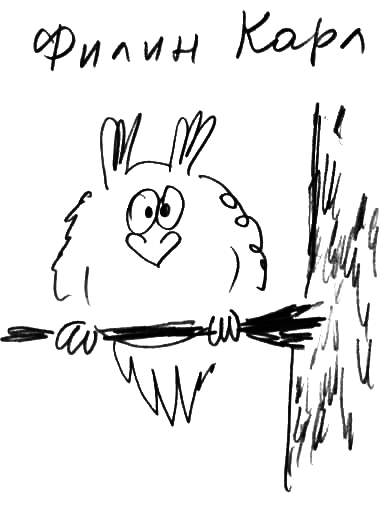
\includegraphics[width=5cm]{images/filin_karl_01.png}
\hspace*{3cm}
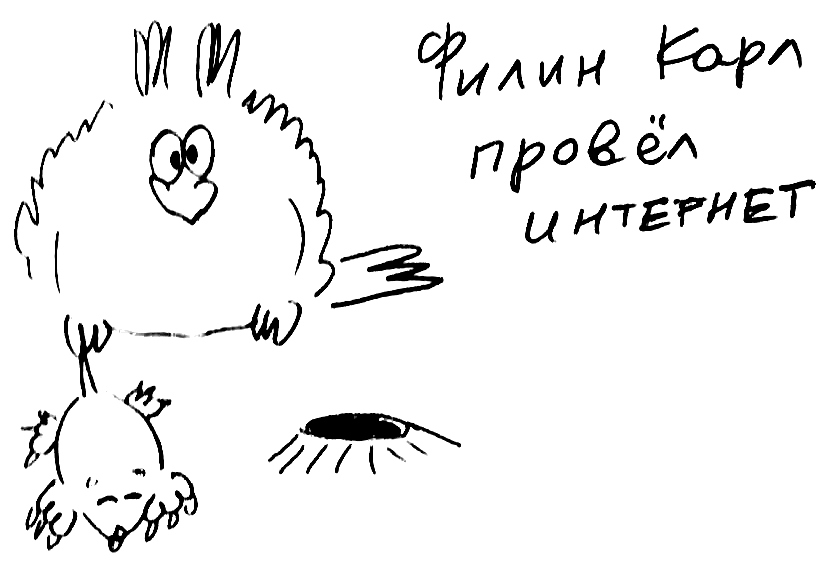
\includegraphics[width=9cm]{images/filin_karl_02.png}

% Задача 9
\item Пусть $X_{1}, \ldots, X_{n}$  — случайная выборка из равномерного распределения на отрезке $[0,\theta]$, где $\theta>0$ — неизвестный параметр распределения. Известно, что $n=100$  и $\bar x=0.57$ . Используя центральную предельную теорему, постройте приближенный 95\%-ый доверительный интервал для параметра $\theta$.

% Задача 10
\item Вовочка любит генерировать случайные числа по поводу и без. 
В этот раз он сгенерировал выборку $x_{1}=-1$, $x_{2}=0$, $x_{3}=1$, и сообщил, 
что данная случайная выборка порождена логистическим распределением с функцией распределения $\Lambda(x)=\frac{e^{x}}{1+e^{x}}$. 

С помощью теста Колмогорова на уровне значимости 1\% проверьте гипотезу о том, 
что данная случайная выборка действительно была получена из логистического распределения. 

\textbf{Подсказка}: $e \approx 2.7$, критическое значение статистики Колмогорова примите равным $0.83$.

\end{enumerate}
	


\subsection[2019-2020]{\hyperref[sec:sol_kr_04_2019_2020]{2019-2020}}
\label{sec:kr_04_2019_2020}



\subsection[2018-2019]{\hyperref[sec:sol_kr_04_2018_2019]{2018-2019}}
\label{sec:kr_04_2018_2019}

Комментарий: минимум писали 30 минут без официальных шпаргалок, основную часть 90 минут — с листом А4. 

\subsubsection*{Минимум}


\begin{enumerate}

%Задача №1
\item Пусть $X_{1}, \ldots, X_{n}$ — случайная выборка из нормального распределения с неизвестным математическим ожиданием $\mu$ и известной дисперсией $\sigma^2=100$. Объем выборки $n=25$. Для тестирования основной гипотезы $H_{0}:\mu=(-1)$ против альтернативы $H_{1}:\mu=0$ Винни-Пух использует простой критерий. Если $\bar X \leq (-0.5)$, то Винни-Пух не отвергает гипотезу $H_{0}$, в противном случае Винни-Пух отвергает гипотезу $H_{0}$ в пользу гипотезы $H_{1}$. 

Найдите:

\begin{enumerate}
    \item вероятность ошибки 1-го рода;
    \item вероятность ошибки 2-го рода;
    \item мощность критерия.
\end{enumerate}

%Задача №2
\item Пусть $X_{1}, \ldots, X_{n}$ — случайная выборка из нормального распределения $\cN(\mu, \sigma^2)$ с неизвестными параметрами $\mu$ и ${\sigma}^2$.
Используя реализацию случайной выборки,
\[
x_{1} = -2, \quad x_{2} = -1, \quad x_{3} = 0, \quad x_{4} = 1, \quad x_{5} = 2
\]
постройте 90\%-ый доверительный интервал для неизвестного параметра $\sigma^2$.

%Задача №3
\item Пусть $X_{1}, \ldots, X_{n}$ и $Y_{1}, \ldots, Y_{m}$ — независимые случайные
выборки из нормальных распределений $\cN(\mu_{X},\sigma^2_{X})$ и
$\cN(\mu_{Y},\sigma^2_{Y})$ соответственно.
Уровень значимости $\alpha = 0.1$.

Используя реализации случайных выборок

\begin{align*}
x_{1} &= -2, \quad x_{2} = -1, \quad x_{3} = 0, \quad x_{4} = 1, \quad x_{5} = 2, \\
y_{1} &= -2, \quad y_{2} = 0, \quad y_{3} = 2,
\end{align*}
проверьте гипотезу о равенстве дисперсий $\sigma^2_X = \sigma^2_Y$ против гипотезы о неравенстве дисперсий.

%Задача №4
\item Пусть $X_{1}, \ldots, X_{n}$ и $Y_{1}, \ldots, Y_{m}$ —
независимые случайные выборки из нормальных распределений 
$\cN(\mu_{X},\sigma^2)$ и $\cN(\mu_{Y},\sigma^2)$ соответственно.

Используя реализации случайных выборок
\begin{align*}
x_{1} &= -2, \quad x_{2} = -1, \quad x_{3} = 0, \quad x_{4} = 1, \quad x_{5} = 2, \\
y_{1} &= -2, \quad y_{2} = 0, \quad y_{3} = 2,
\end{align*}
постройте 60\%-ый доверительный интервал для разности математических ожиданий
$\mu_{X} - \mu_{Y}$.

%Задача 5
\item Пусть $X_{1}, \ldots, X_{n}$ и $Y_{1}, \ldots, Y_{m}$ — две независимые случайные выборки из распределения Бернулли с неизвестными параметрами $p_{X}\in(0,1)$ и $p_{Y}\in(0,1)$. Известно, что $n=100$, $m=150$, $\sum_{i=1}^{n}x_{i}=60$, $\sum_{i=1}^{n}y_{i}=50$. На уровне значимости $\alpha=0.05$ протестируйте гипотезу $H_{0}:p_{X}=p_{Y}$ против альтернативной гипотезы $H_{1}:p_{X}>p_{Y}$.


\end{enumerate}

\subsubsection*{Основная часть}


\begin{enumerate}

%Задача №1

\item Пусть $X$ — случайная выборка, содержащая одно наблюдение, из распределения с функцией плотности

\[
f_X(x) =
	\begin{cases}
	\theta x^{\theta-1},\text{ при }  x \in [0; 1] \\
	0\quad \quad \text{, }\text{ при } x \notin  [0; 1] \\
	\end{cases},
\]

где $\theta>0$ — неизвестный параметр распределения. Тестируется основная гипотеза $H_{0}:\theta=1$ против альтернативной гипотезы $H_{1}:\theta=2$.

\begin{enumerate}
    \item (7) С помощью леммы Неймана–Пирсона найдите наиболее мощный критерий, имеющий уровень значимости $\alpha=0.05$.
    \item (3) Вычислите мощность полученного критерия.
\end{enumerate}

%Задача №2

\item На раскопках старинного замка Вася нашел древнюю монетку. Монетка ему показалась крайне необычной, и поэтому он решил провести серию из 100 подбрасываний. Результаты Вася записал в таблицу.

\begin{center}\begin{tabular}{rrrr}
\toprule
   & Орел   & Решка & Ребро  \\ \midrule
Количество раз &   $40$ & $50$ & $10$ \\ \bottomrule
\end{tabular}\end{center}
\begin{enumerate}
    \item (6) Постройте двусторонний 95\%-ый доверительный интервал для вероятности выпадения ребра.
    \item (4) На уровне значимости 5\% проверьте гипотезу о том, что ребро выпадает в одном случае из 100 против альтернативы, что чаще, и вычислите соответствующее $P$-значение.
    \item (10) С помощью теста отношения правдоподобия на уровне значимости 10\% проверьте гипотезу о том, что орёл выпадает так же часто, как решка, и в три раза чаще, чем ребро.
    \item (5) С помощью критерия согласия Пирсона на уровне значимости 10\% проверьте гипотезу из предыдущего пункта.
\end{enumerate}

Подсказка: $\ln 2 \approx 0.7$, $\ln 3 \approx 1.1$, $\ln 5 \approx 1.6$, $\ln 7 \approx 1.95$, $\ln 11 \approx 2.4$.

%Задача №3

\item Губка Боб и Патрик ловят медуз для коллекции. Число пойманных за $i$-ый день медуз имеет распределение Пуассона с неизвестным параметром $\lambda$. Уловы медуз в различные дни независимы. За прошедшие $100$ дней они поймали $300$ медуз. 

\begin{enumerate}
    \item (5) С помощью асимптотических свойств оценок максимального правдоподобия постройте 95\%-ый доверительный интервал для неизвестного параметра $\lambda$.
    \item (10) С помощью дельта-метода постройте приближенную 95\%-ую интервальную оценку вероятности того, что за 101-ый день Губка Боб и Патрик не поймают ни одной медузы.
\end{enumerate}

\end{enumerate}





\subsection[2017-2018]{\hyperref[sec:sol_kr_04_2017_2018]{2017-2018}}
\label{sec:kr_04_2017_2018}


\subsubsection*{Минимум}

\begin{enumerate}


	\item Пусть $X=(X_{1}, \ldots,X_{n})$ — случайная выборка из нормального распределения с неизвестным математическим ожиданием $\mu$ и неизвестной дисперсией $\sigma^2=9$. Объем выборки $n=20$. Для тестирования основной гипотезы $H_{0}:\mu=0$ против альтернативной гипотезы $H_{1}:\mu=5$ вы используете критерий: если $\overline{X}\leq2$, то вы не отвергаете гипотезу $H_{0}$, в противном случае вы отвергаете гипотезу $H_{0}$ в пользу гипотезы $H_{1}$. Найдите
	\begin{enumerate}
	\item Вероятность ошибки 1-го рода
	\item Вероятносто ошибки 2-го рода
	\end{enumerate}


		\item Пусть $X=(X_{1}, \ldots,X_{n})$ — случайная выборка из нормального распределения с неизвестными параметрами $\mu$ и $\sigma^2$. Используя реализацию случайной выборки: $x_{1}=2$, $x_{3}=8$, $x_{3}=5$, постройте 95\%-ый доверительный интервал для неизвестного параметра $\sigma^2$.


	\item Вася очень любит тестировать статистические гипотезы. В этот раз Вася собирается проверить утверждение о том, что его друг Пётр звонит Васе исключительно в то время, когда Вася ест. Для этого Вася трудится целый год и проводит серию из 365 испытаний. Результаты приведены в табилце ниже.

	\begin{center}
		\begin{tabular}{c|cc}
			\toprule
			& Пётр не звонит & Пётр звонит\\
			\midrule
			Вася ест & $100$ & $50$\\
			Вася не ест  & $125$ & $90$\\
			\bottomrule
		\end{tabular}
	\end{center}

	На уровне значимости 10\% протестируйте гипотезу о том, что Пётр звонит Васе независимо от момента приема пищи.


\item Вася Сидоров утверждает, что ходит в кино в четыре раза чаще, чем в спортзал, а в спортзал в четыре раза чаще, чем в театр.
За последние полгода он 105 раз был в театре, 63 раза — в спортазе и 42 раза в кино.
На уровне значимости 10\% проверьте утверждение Васи.

\end{enumerate}


	\begin{center}
	Квантили $\chi^2$ распределения c 1, 2 и 3 степенями свободы\\
		\begin{tabular}{c|cccccc}
			\toprule
			& 0.025 & 0.05 & 0.1 & 0.9 & 0.95 & 0.975\\
			\midrule
							1 & 0.001 & 0.004 & 0.016 & 2.706 & 3.841 & 5.024 \\
							2 & 0.051 & 0.103 & 0.211 & 4.605 & 5.991 & 7.378 \\
							3 & 0.216 & 0.352 & 0.584 & 6.251 & 7.815 & 9.348 \\
			\bottomrule
		\end{tabular}
	\end{center}

\newpage

\subsubsection*{Задачи}

При решении задач пять–семь используйте данные обследования Росстата за первый квартал 2018 года:

	\begin{center}
		\begin{tabular}{c|ccc}
			\toprule
			& Число наблюдений & Среднее (тыс. руб.) & Выборочное отклонение (тыс. руб.) \\
			\midrule
							Врачи & 40 & 136 & 55  \\
							Преподаватели & 60 & 139 & 60 \\
			\bottomrule
		\end{tabular}
	\end{center}

Распределение заработной платы работников любой отрасли хорошо описывается нормальным законом.

\begin{enumerate}[resume]

	%Задача 1
	\item На уровне значимости 5\% проверьте гипотезу о том, что средняя зарплата врача составляет 100 т.р., против альтернативы, что она больше 100 т.р.  Вычислите минимальный уровень значимости, при котором основная гипотеза отвергается (Р–значение).

	%Задача 2
	\item На уровне значимости 10\% проверьте гипотезу о том, что разброс в зарплатах врачей и преподавателей одинаков, против двухсторонней альтернативы.

	%Задача 3
	\item На уровне значимости 10\% проверьте гипотезу о том, что средняя зарплата врачей и преподавателей совпадают, против альтернативы, что у преподавателей зарплата выше:

	\begin{enumerate}
	\item Считая объемы выборок достаточно большими
			\item Считая дисперсии одинаковыми
	 \end{enumerate}

			%Задача 4
			\item Время в часах безотказной работы  микронаушника, величина $X$, подчиняется экспоненциальному (показательному) закону распределения с неизвестным параметром $\lambda$:
\[
f(x;\lambda)
			=\begin{cases}
			\lambda e^{-\lambda x},\text{ при } x\geq0\\
			0, \text{ при }  x<0\\
			\end{cases}
\]
По выборке из 100 независимых наблюдений $\bar x=0.52$. С помощью асимптотических свойств оценок максимального правдоподобия постройте приближенный 95\%-ый доверительный интервал:

\begin{enumerate}
	\item Для параметра $\lambda$
			\item Для вероятности того, что наушник проработает без сбоев весь тест — 45 минут
	 \end{enumerate}

	 %Задача 5
	 \item Приглашенный на Петербургский международный экономический форум Германом Грефом индийский мистик Садхгуру подарил Грефу древнюю шестигранную кость для принятия решений в сложных макроэкономических ситуациях. Служба безопасности Сбербанка провела серию из 100 испытаний и составила таблицу:

			 \begin{center}
		\begin{tabular}{c|cccccc}
			\toprule
			Грань & 1 & 2 & 3 & 4 & 5 & 6\\
			\midrule
							Число выпадений & 10 & 10 & 15 & 15 & 25 & 25 \\
			\bottomrule
		\end{tabular}
	\end{center}

С помощью теста отношения правдоподобия на уровне значимости 5\% проверьте гипотезу о том, что все грани равновероятны.

\[
\ln(1/6)=-1.79, \; \ln(0.15)=-1.90, \; \ln(0.25)=-1.39, \; \ln(0.1)=-2.30
\]

\end{enumerate}


\newpage
\subsection[2016-2017]{\hyperref[sec:sol_kr_04_2016_2017]{2016-2017}}
\label{sec:kr_04_2016_2017}


\subsubsection*{I. Теоретический минимум}


В пунктах 1, 3, 11 и 12 предполагается, что $X = (X_1, \, \ldots, \, X_n)$ и
$Y = (Y_1, \, \ldots, \, Y_m)$ — две независимые случайные выборки из нормальных
распределений $N(\mu_X, \sigma_X^2)$ и $N(\mu_Y, \sigma_Y^2)$ соответственно.

\begin{enumerate}
  \item Приведите формулу статистики, при помощи которой можно проверить гипотезу
	$H_0 \colon \sigma_X^2 = \sigma_Y^2$. Укажите распределение этой статистики при
	верной гипотезе $H_0$.
  \item Приведите формулу информации Фишера о параметре $\theta$, содержащейся в
	одном наблюдении случайной выборки.
  \item Приведите формулу статистики, при помощи которой можно проверить гипотезу
	$H_0 \colon \mu_X - \mu_Y = \Delta_0$ при условии, что дисперсии $\sigma_X^2$
	и $\sigma_Y^2$ неизвестны, но равны между собой. Укажите распределение этой
	статистики при верной гипотезе $H_0$.
  \item Дайте определение критической области.
  \item Приведите формулу плотности нормального распределения $\cN(\mu, \sigma^2)$.
  \item Приведите формулы границ доверительного интервала с уровнем доверия
	$(1 - \alpha)$, $\alpha \in (0;\,1)$, для вероятности появления успеха в
	случайной выборке $X = (X_1, \, \ldots, \, X_n)$ из распределения Бернулли с
	параметром $p \in (0;\,1)$.
  \item Дайте определение несмещенной оценки $\hat{\theta}$ для неизвестного
	параметра $\theta \in \Theta$.
  \item Дайте определение эффективной оценки $\hat{\theta}$ для неизвестного
	параметра $\theta \in \Theta$.
  \item Приведите формулу выборочной дисперсии.
  \item Приведите формулу выборочной функции распределения.
  \item Приведите формулы границ доверительного интервала с уровнем доверия
	$(1 - \alpha)$, $\alpha \in (0;\,1)$, для $\mu_X$ при условии, что дисперсия
	$\sigma_X^2$ известна.
  \item Укажите распределение статистики $\frac{\overline{X} - \mu_X}{\sigma / \sqrt{n}}$.
\end{enumerate}


\subsubsection*{II. Задачи}

\begin{enumerate}
\item В ходе анкетирования ста сотрудников банка «Альфа» были получены ответы на
вопрос о том, сколько времени они проводят на работе ежедневно. Среднее выборочное
оказалось равным $9.5$ часам, а выборочное стандартное отклонение $0.5$ часа.
\begin{enumerate}
  \item На уровне значимости 5\,\% проверьте гипотезу о том, что сотрудники банка
	«Альфа» в среднем проводят на работе $10$ часов, против альтернативной гипотезы о
	том, что сотрудники банка «Альфа» в среднем проводят на работе менее $10$ часов.
  \item Найдите точное $P$-значение для наблюдаемой статистики из пункта (a).
  \item Сформулируйте предпосылки, которые были использованы вами для выполнения
	пункта (a).
  \item На уровне значимости 5\,\% проверьте гипотезу о $H_0 \colon \sigma^2 = 0.3$.
\end{enumerate}


\item Проверка сорока случайно выбранных лекций показала, что студент Халявин
присутствовал только на 16 из них. На уровне значимости 5\,\% проверьте гипотезу
о том, что Халявин посещает в среднем половину лекций.

\item В ходе анкетирования двадцати сотрудников банка «Альфа» были получены ответы
на вопрос о том, сколько времени они проводят на работе ежедневно. Среднее выборочное
оказалось равным $9.5$ часам, а выборочное стандартное отклонение $0.5$ часа.
Аналогичные показатели для 25 сотрудников банка «Бета» составили $9.8$ и $0.6$
часа соответственно.
\begin{enumerate}
  \item На уровне значимости 5\,\% проверьте гипотезу о равенстве математических
	ожиданий времени, проводимого на работе сотрудниками банков «Альфа» и «Бета».
  \item Сформулируйте предпосылки, которые были использованы вами для выполнения
	пункта (a).
  \item На уровне значимости 5\,\% проверьте гипотезу о равенстве дисперсий времени,
	проводимого на работе сотрудниками банков «Альфа» и «Бета».
\end{enumerate}

\item Вася решил проверить известное утверждение о том, что бутерброд падает
маслом вниз. Для этого он провел серию из 200 испытаний. Ниже приведена таблица
с результатами:
\begin{center}
\begin{tabular}{ccc}
  \toprule
  \text{Бутерброд}                &\text{Маслом вниз}    &\text{Маслом вверх}       \\ \midrule
  \text{Число наблюдений}         &$105$    &$95$       \\ \bottomrule
\end{tabular}
\end{center}
Можно ли утверждать, что бутерброд падает маслом вниз так же часто, как и маслом
вверх? При ответе на вопрос используйте уровень значимости 5\,\%.

\item Пусть $X = (X_1, \, \ldots, \, X_{100})$ — случайная выборка из нормального
распределения с математическим ожиданием $\mu$ и дисперсией $\nu$. Оба параметра
$\mu$ и $\nu$ неизвестны. Используя следующие данные $\sum_{i=1}^{100}x_i = 30$,
$\sum_{i=1}^{100}x_i^2 = 146$ и $\sum_{i=1}^{100}x_i^3 = 122$ с помощью теста
отношения правдоподобия проверьте гипотезу $H_0 \colon \nu = 1$ на уровне значимости 5\,\%.
\end{enumerate}


\newpage
\subsection[2015-2016]{\hyperref[sec:sol_kr_04_2015_2016]{2015-2016}}
\label{sec:kr_04_2015_2016}

\begin{enumerate}
\item	Сформулируйте определения несмещённости, состоятельности и эффективности оценок.
\item На курсе учится 250 человек. Предположим, что число студентов, не явившихся
на экзамен, хорошо описывается законом Пуассона.
\begin{enumerate}
\item	Методом максимального правдоподобия найдите оценку параметра распределения Пуассона.
\item	Проверьте выполнение свойств несмещенности, эффективности и состоятельности
для данной оценки.
\item	Найдите оценку максимального правдоподобия для вероятности стопроцентной
явки студентов на экзамен.
\item	Используя дельта-метод, постройте для этой вероятности асимптотический
доверительный интервал.
\end{enumerate}

\item	Фармацевтическая компания выпустила новое лекарство от бессонницы, утверждая,
что оно помогает 80\% людей, страдающих бессонницей. Чтобы проверить утверждение
компании, случайным образом выбираются 20 человек, страдающих бессонницей. Обозначим
за $Y$ количество человек из выборки, которым лекарство помогло. Основная гипотеза,
$H_0$: $p=0.8$, альтернативная гипотеза $H_a$: $p=0.6$. Критическая область: $\{Y<12\}$.
\begin{enumerate}
\item	В терминах этой задачи сформулируйте, что является ошибкой первого рода.
Найдите уровень значимости, соответствующий заданной критической области.
\item	В терминах этой задачи сформулируйте, что является ошибкой второго рода.
Найдите вероятность ошибки второго рода.
\item	Найдите такое значение $c$, что вероятность ошибки первого рода $\alpha
\approx 0.1$ при критической области вида $\{Y<c\}$. Найдите соответствующее
значение вероятности ошибки второго рода.
\item	Каким должен быть размер выборки, чтобы выборочная доля страдающих бессонницей
отличалась от истинной вероятности не более, чем на $0.01$ с вероятностью не менее,
чем $0.95$?
\end{enumerate}

\item	Вася Сидоров утверждает, что ходит в кино в два раза чаще, чем на лекции
по статистике, на лекции по статистике в два раза чаще, чем в спортзал. За
последние полгода он 10 раз был в спортзале, 1 раз — на лекциях по статистике и
39 раз в кино.

При помощи критерия хи-квадрат Пирсона на уровне значимости $0.05$ проверьте,
правдоподобно ли Васино утверждение.

\item У Евдокла есть случайная выборка из экспоненциального распределения с
неизвестным параметром $\lambda$ в 50 наблюдений, $X_1$, $X_2$, \ldots, $X_{50}$.
Оказалось, что $\bar X = 1.1$. Евдокл хочет проверить гипотезу о равенстве
$\lambda = 1$ против альтернативной гипотезы о неравенстве $\lambda \neq 1$ на
уровне значимости $0.1$.

Помогите Евдоклу и проверьте гипотезу с помощью критерия отношения правдоподобия.

Пачка логарифмов: $\ln 50 \approx 3.9$, $\ln 55 \approx 4.0$, $\ln 11 \approx 2.4$,
$\ln 60 \approx 4.1$, $\ln 12 \approx 2.5$

\item Американский демографический журнал опубликовал исследование, в котором
утверждается, что посетители крупных торговых центров за одно посещение тратят
в выходные дни больше, чем в будние. Наибольшие расходы приходятся на воскресенье
в период с 4 до 6 часов вечера. Для двух независимых выборок посетителей средние
расходы и выборочные стандартные отклонения расходов составили
\begin{center}
\begin{tabular}{lrr}
\toprule
 & Выходные & Рабочие дни \\
\midrule
Число наблюдений & 21 & 19 \\
Средние расходы (\$) & 78 & 67 \\
Выборочное стандартное отклонение (\$) & 22 & 20 \\
\bottomrule
\end{tabular}
\end{center}

\begin{enumerate}
\item Проверьте гипотезу о равенстве дисперсий расходов
\item Предполагая, что дисперсии расходов одинаковы, проверьте гипотезу об отсутствии
разницы в расходах в выходные и будние дни.
\item Сформулируйте все необходимые для проверки гипотез предыдущих пунктов предпосылки.
\end{enumerate}

\item Винни Пух знает, что пчёлы и мёд бывают правильные и неправильные.
По результатам 100~попыток добыть мёд Винни Пух составил таблицу сопряженности признаков.

\begin{center}
\begin{tabular}{lrr}
\toprule
 & Мёд правильный & Мёд неправильный \\
\midrule
Пчёлы правильные & 12	& 36 \\
Пчёлы неправильные & 32	& 20 \\
\bottomrule
\end{tabular}
\end{center}

На уровне значимости $0.05$ проверьте гипотезу о независимости характеристик пчёл и мёда.

\begin{figure}[b]
\centering
\includegraphics[width=9cm]{images/winnie_kr_4}
\end{figure}
\end{enumerate}



\newpage
\subsection[2014-2015]{\hyperref[sec:sol_kr_04_2014_2015]{2014-2015}}
\label{sec:kr_04_2014_2015}

\begin{enumerate}

\item[1.] \textbf{Задача для первого потока.}

Проверка 40 случайно выбранных лекций показала, что студент Халявин присутствовал
только на 16 из них.
\begin{enumerate}
\item Найдите 95\% доверительный интервал для вероятности увидеть Халявина на лекции.
\item На уровне значимости 5\% проверьте гипотезу о том, что Халявин посещает
в среднем половину лекций.
\item Вычислите минимальный уровень значимости, при котором основная гипотеза
отвергается (P-значение).
\end{enumerate}

\item[1.] \textbf{Задача для второго потока.}

Вес упаковки с лекарством является нормальной случайной величиной.
Взвешивание 20~упаковок показало, что выборочное среднее равно 51 г., а
несмещенная оценка дисперсии равна~4.
\begin{enumerate}
\item На уровне значимости 10\% проверьте гипотезу, что в среднем вес упаковки
составляет~55 г.
\item Контрольное взвешивание 30 упаковок такого же лекарства другого производителя
показало, что несмещенная оценка дисперсии веса равна 6. На уровне значимости 10\%
проверьте гипотезу о равенстве дисперсий веса упаковки двух производителей.
\end{enumerate}

\item[2.] \textbf{Задача для первого потока.}

В ходе анкетирования 15 сотрудников банка «Альфа» ответили на вопрос о том,
сколько времени они проводят на работе ежедневно. Среднее выборочное оказалось
равно $9.5$ часам при выборочном стандартном отклонении $0.5$ часа. Аналогичные
показатели для 12 сотрудников банка «Бета» составили $9.8$ и $0.6$ часа соответственно.

Считая распределение времени нормальным, на уровне значимости 5\% проверьте
гипотезу о том, что сотрудники банка «Альфа» в среднем проводят на работе столько
же времени, сколько и сотрудники банка «Бета».

\item[2.] \textbf{Задача для второго потока.}

Экзамен принимают два преподавателя, случайным образом выбирая студентов.
По выборке из 85 и 100 наблюдений, выборочные доли не сдавших экзамен студентов составили
соответственно $0.2$ и $0.17$.
\begin{enumerate}
\item Можно ли при уровне значимости в 1\% утверждать, что преподаватели предъявляют
к студентам одинаковый уровень требований?
\item Вычислите минимальный уровень значимости, при котором основная гипотеза
отвергается (P-значение).
\end{enumerate}

\item[3.] Методом максимального правдоподобия найдите оценку параметра $\theta$
для выборки $X_1$, \ldots, $X_n$ из распределения с функцией плотности
\[
f(x)=\begin{cases}
\frac{1}{\theta^2}xe^{-\frac{x}{\theta}}, \; x>0 \\
0, \; x\leq 0
\end{cases}
\]

\item[4.]
Пусть $X_1$, \ldots, $X_{100}$ — случайная выборка из нормального распределения
с математическим ожиданием $\mu$ и дисперсией $\nu$, где $\mu$ и $\nu$ — неизвестные
параметры. По 100 наблюдениям $\sum x_i=30$, $\sum x_i^2=146$, $\sum x_i^3=122$.

При помощи теста отношения правдоподобия протестируйте гипотезу $H_0: \nu=1$
на уровне значимости 5\%.

\item[5.] \textbf{Исследовательская задача.}

Пусть $X_1$, \ldots, $X_{n}$ — случайная выборка из нормального распределения
с математическим ожиданием $\mu$ и дисперсией $\nu$, где $\mu$ и $\nu$ — неизвестные
параметры. Рассмотрим три классических теста, отношения правдоподобия, $LR$,
множителей Лагранжа, $LM$ и Вальда, $W$, для тестирования гипотезы $H_0: \; \mu=0$.

\begin{enumerate}
\item Сравните  статистики $LR$, $LM$ и $W$ между собой. Какая — наибольшая,
какая — наименьшая?
\item Изменится ли упорядоченность статистик, если проверять гипотезу $H_0: \; \mu=\mu_0$?
\end{enumerate}

Подсказка: $\frac{x}{1+x} \leq \ln(1+x) \leq x\, \; \text{ при } x>-1$

\item[6.] \textbf{Исследовательская задача.}

Величины $X_1$, \ldots, $X_n$ независимы и одинаково распределены с функцией плотности
\[
f(x)=\begin{cases}
a^2xe^{-ax}, \; x>0 \\
0, \; x\leq 0
\end{cases}
\]

По выборке из 100 наблюдений оказалось, что $\sum x_i =300$, $\sum x_i^2=1000$,
$\sum x_i^3=3700$.

\begin{enumerate}
\item Найдите оценку неизвестного параметра $a$ методом моментов
\item Используя дельта-метод или иначе оцените дисперсию полученной оценки $a$
\item Постройте 95\%-ый доверительный интервал используя оценку метода моментов
\end{enumerate}
\end{enumerate}



\subsection[2009-2010]{\hyperref[sec:sol_kr_04_2009_2010]{2009-2010}}
\label{sec:kr_04_2009_2010}



\begin{enumerate}

\item Сколько нужно бросить игральных костей, чтобы вероятность выпадения хотя бы одной шестерки была не меньше $0.9$?
\item Снайпер попадает в «яблочко» с вероятностью 0.8, если он в предыдущий выстрел попал в «яблочко» и с вероятностью 0.7, если в предыдущий раз не попал в  «яблочко». Вероятность попасть в «яблочко» при первом выстреле также 0.7. Снайпер стреляет 2 раза.
\begin{enumerate}
\item Определите вероятность попасть в «яблочко» при втором выстреле
\item Какова вероятность того, что снайпер попал в «яблочко» при первом выстреле, если известно, что он попал при втором?
\end{enumerate}

\item Случайная величина $X$ моделирует время, проходящее между двумя телефонными звонками в справочную службу. Известно, что $X$ распределена экспоненциально со стандартным отклонением равным 11 минутам. Со времени последнего звонка прошло 5 минут. Найдите функцию распределения и математическое ожидание времени, оставшегося до следующего звонка.

\item Известно, что для двух случайных величин $X$ и $Y$: $\E(X)=1$, $\E(Y)=2$, $\E(X^2)=2$, $\E(Y^2)=8$, $\E(XY)=1$.
\begin{enumerate}
\item Найдите ковариацию и коэффициент корреляции величин $X$ и $Y$.
\item Определите, зависимы ли величины $X$ и $Y$.
\item Вычислите дисперсию их суммы.
\end{enumerate}

\item Предположим, что время «жизни» $X$ энергосберегающей лампы распределено по нормальному закону. По 10 наблюдениям среднее время «жизни» составило 1200 часов, а выборочное стандартное отклонение 120 часов.
\begin{enumerate}
\item Постройте двусторонний доверительный интервал для математического ожидания величины $X$ с уровнем доверия 0.90.
\item Постройте двусторонний доверительный интервал для стандартного отклонения величины $X$ с уровнем доверия 0.80.
\item Какова вероятность, что несмещенная оценка для дисперсии, рассчитанная по 20 наблюдениям, отклонится от истинной дисперсии меньше, чем на 40\%?
\end{enumerate}

\item Учебная часть утверждает, что все три факультатива «Вязание крючком для экономистов», «Экономика вышивания крестиком» и «Статистические методы в макраме» одинаково популярны. В этом году на эти факультативы соответственно записалось 35, 31 и 40 человек. Правдоподобно ли заявление учебной части?
\item Имеются две конкурирующие гипотезы:
\begin{enumerate}
\item[$H_0$:] Случайная величина X распределена равномерно на (0,100);
\item[$H_a$:] Случайная величина X распределена равномерно на (50,150).
\end{enumerate}
Исследователь выбрал следующий критерий: если $X<c$, принимать гипотезу $H_0$, иначе  $H_a$.
\begin{enumerate}
\item Дайте определение «ошибки первого рода», «ошибки второго рода», «мощности критерия».
\item Постройте графики зависимости вероятностей ошибок первого и второго рода от $c$.
\item Вычислите $c$ и вероятность ошибки второго рода, если уровень значимости критерия равен 0.05.
\end{enumerate}
\item Из 10 опрошенных студентов часть предпочитала готовиться по синему учебнику, а часть по зеленому. В таблице представлены их итоговые баллы.

\begin{tabular}{@{}lcccccc@{}}
\toprule
Синий   & 76 & 45 & 57 & 65 &    &    \\
Зелёный & 49 & 59 & 66 & 81 & 38 & 88 \\ \bottomrule
\end{tabular}


С помощью теста Манна-Уитни (Вилкоксона) проверьте гипотезу о том, что выбор учебника не меняет закона распределения оценки.

\item Случайная величина $X$, характеризующая срок службы элементов электронной аппаратуры, имеет распределение Релея: $F(x)=1-e^{-x^2/\theta}$ при $x\geq 0$. По случайной выборке $X_1$, $X_2$, ..., $X_n$ найдите оценку максимального правдоподобия параметра $\theta$.

\item По случайной выборке $X_1$, $X_2$, \ldots, $X_n$ из равномерного на интервале $[\theta;\theta+10]$ распределения методом моментов найдите оценку параметра $\theta$. Дайте определение несмещенности и состоятельности оценки и определите, будет ли обладать этими свойствами найденная оценка.

\item При расчете страхового тарифа страховая компания предполагает, что вероятность наступления страхового случая 0.005. По итогам прошедшего года из 10000 случайно выбранных договоров страховых случаев наблюдалось 67.
\begin{enumerate}
\item Согласуются ли полученные данные с предположением страховой компании? Альтернативная гипотеза: вероятность страхового случая больше.
\item Определить минимальный уровень значимости, при котором основная гипотеза отвергается.
\end{enumerate}
\end{enumerate}

% !TEX root = ../probability_hse_exams.tex
\newpage
\thispagestyle{empty}
\section{Контрольная работа 4. ИП}

\subsection[2023-2024]{\hyperref[sec:sol_kr_04_ip_2023_2024]{2023-2024}}
\label{sec:kr_04_ip_2023_2024}

Очно, 70 минут, можно было использовать шпаргалку А4.

\begin{enumerate}
\item  В течение двух дней проводился опрос населения города с целью определения отношения жителей к действующей администрации. 
В первый день было опрошено 256 человек. 
По этим данным статистик построил доверительный интервал для доли тех, 
кто выразил положительное отношение к работе администрации города: $[31,57\%; 43,43\%]$.
Во второй день были опрошены ещё 144 человека, из которых 46 выразили положительное
отношение к работе администрации.
\begin{enumerate}
\item  (8) Какой уровень доверия (доверительная вероятность) использовался при
построении доверительного интервала по данным первого дня опроса?
\item  (8) По данным за оба дня рассчитайте 90\% доверительный интервал для
доли населения, положительно относящегося к работе администрации.
\item  (10) По данным за второй день на уровне значимости $0.05$ проверьте
гипотезу о том, что менее половины жителей положительно оценивают
работу администрации. 
Сформулируйте основную и альтернативную гипотезы (1), выпишите тестовую статистику (3), 
задайте критическую область (2), сделайте вывод (1). 
Вычислите $p$-значение (3).
\item (10) По данным за второй день найдите оценку
вероятности того, что в выборке из 10 жителей ровно 5 человек положительно оценят администрацию (3).
С помощью дельта-метода найдите асимптотическую дисперсию этой оценки (4) и постройте 95\%-й асимптотический доверительный интервал (3) для указанной вероятности.
\end{enumerate}

\item  (20) Случайные выборки $X_1$, \ldots, $X_n$ и $Y_1$, \ldots, $Y_m$ независимы и имеют нормальные распределения  $X_i \sim \cN(\mu_X, \sigma_X^2)$ и $Y_j \sim \cN(\mu_Y, \sigma_Y^2)$.
Известно, что $\sum_{i=1}^{10} X_i^2=385$, $\sum_{i=1}^{10} X_i=55$, $\sum_{i=1}^{10} Y_i^2=323$, $\sum_{i=1}^{10} Y_i=49$.

\begin{enumerate}
    \item (8) Постройте 90\%-й доверительный интервал для отношения дисперсий.
    \item  (5) Предположим, что истинная дисперсия в выборке $X$ известна и равна $\sigma_x^2 = 10$. 
    С какой вероятностью выборочная дисперсия $\hat{\sigma_x}^2$ будет не менее 5. 
\item  (10) Проверьте гипотезу о равенстве математических ожиданий  $H_0: \mu_x = \mu_y$
с предположением о равенстве дисперсий и без него, используя статистику Уэлча.
\end{enumerate}

\item (15) Есть случайная выборка из 5 наблюдений с распределением Бернулли.
С помощью леммы Неймана~— Пирсона постройте рандомизированный наиболее мощный критерий с уровнем значимости $0.01$ (10) для проверки гипотезы $H_0: p=\frac{1}{2}$ против альтернативы $H_1: p=\frac{2}{3}$.
Найдите  мощность построенного критерия (5).

\item (16) Игральная кость в форме тетраэдра подбрасывается 100 раз. 
Различные грани тетраэдра выпадали $25$, $18$, $30$ и $27$ раз. 
С помощью критерия отношения правдоподобия на уровне значимости $0.05$ проверьте гипотезу о том, 
что тетраэдр правильный (12). 
Проверьте эту гипотезу любым альтернативным способом (4).


\item (15) По выборке $X_1$, \ldots, $X_n$ из распределения $F_0$ построена эмпирическая функция распределения $\hat F_n$ и статистика $D_n=\max_x \abs{\hat F_n(x)-F_0(x)}$. 
Докажите, что распределение статистики $D_n$ не зависит от $F_0$.

\end{enumerate}


\subsection[2018-2019]{\hyperref[sec:sol_kr_04_ip_2018_2019]{2018-2019}}
\label{sec:kr_04_ip_2018_2019}

Ровно 189 лет назад, 1 июня 1830 британский учёный Джон Росс открыл северный магнитный полюс :)


\begin{enumerate}
\item Пусть $y$ — стандартный нормальный $n$-мерный вектор. 
Он случайный, просто Джону Россу лень писать заглавные буквы для векторов :) 
Вектор $a$ — неслучайный, но тоже гордый $n$-мерный.

Пусть $H$ — матрица, проецирующая любой вектор на $(n-1)$-мерное подпространство $a^{\perp}$, 
являющееся ортогональным дополнением к вектору $a$. 
То есть, для любого вектора $v$ вектор $Hv$ перпендикулярен вектору $a$.

\begin{enumerate}
    \item Найдите матрицу $H$, если $n=3$ и $a=(1,2,2)'$.
    \item Найдите матрицу $H$ для произвольного $n$ и $a$;
    \item Найдите $\E(y)$ и $\Var(y)$;
    \item Найдите $\E(Hy)$ и $\Var(Hy)$;
    \item Укажите закон распределения $y'Hy$, где $y'$ — это транспонированный вектор $y$.
\end{enumerate}

\item Рассмотрим формулу, здорово упрощающую подсчёт критерия Пирсона:
\[
 \sum_{j=1}^m \frac{(X_j - np_j)^2}{np_j} + n = \sum_{j=1}^m \frac{X_j^2}{np_j}
\]

\begin{enumerate}
    \item Докажите формулу.
    \item Нарисуйте картинку к этой формуле. На картинке подпишите прямой угол, катеты и гипотенузу. 
    Явно запишите каждый вектор. Объясните, почему треугольник, действительно, прямоугольный. 
\end{enumerate}


\item На Земле короля Уильяма Джон Росс нашёл странную монетку. 
Он подбрасывает её $n$ раз и обнаруживает, что она выпадает на орла, решку и ребро. 
Джон Росс проверяет гипотезу $H_0$ о том, что все три вероятности равны.

Пусть $y = (y_1, y_2, y_3)'$ — количество выпадений орла, решки и ребра. Рассмотрим так же вектор
$z = (z_1, z_2, z_3)'$, такой, что $z_i = (y_i - \E(y_i)) / \sqrt{\E(y_i)}$. 
Джон Росс сознательно перепутал ожидание и дисперсию в классической формуле!

Предположим, что гипотеза $H_0$ верна.
\begin{enumerate}
    \item Укажите закон распределения каждой величины $y_i$;
    \item Найдите вектор $\E(y)$ и матрицу $\Var(y)$;
    \item Найдите вектор $\E(z)$ и матрицу $\Var(z)$;
    \item Докажите, что матрица $H=\Var(z)$ является проектором на ортогональное дополнение к некоторому вектору $a$. 
  Явно выпишите вектор $a$.
  \item Объясните, почему критерий Пирсона имеет хи-квадрат распределение с нужным числом степеней свободы.
  % \item Обобщите решение на случай прозвольных вероятностей или произвольного количества граней у монетки.
\end{enumerate}

\newpage

\item На Земле короля Уильяма Джон Росс нашёл странную монетку. 
Он подбрасывает её $n$ раз и обнаруживает, что она выпадает на орла, решку и ребро. 
Джон Росс проверяет гипотезу о том, что все три вероятности равны с помощью двух статистики: 
$LR$, отношения правдоподобия, и $CP$, критерия Пирсона. 

\begin{enumerate}
\item Найдите $\plim_{n\to\infty} \frac{LR}{CP}$;
\item Обобщите решение на случай произвольного количества равновероятных граней у монетки.    
% \item Обобщите решение на случай произвольного количества граней и произвольных вероятностей в гипотезе $H_0$.
\end{enumerate}

\item Идея доказательства состоятельности ML оценки :)

Пусть наблюдения $y_1$, \ldots, $y_n$ независимы и одинаково распределены с функцией плотности, зависящей от параметра $a$.
Истинное значение параметра обозначим буквой $a_0$. Оценку максимального правдоподобия обозначим $\hat a$.

Рассмотрим отмасштабированную логарифмическую функцию правдоподобия $\ell_n(a)=\ell(a) / n$, и
ожидаемую логарифмическую функцию правдоподобия\footnote{Внимание:
ожидание считается с помощью истинного $a_0$ от функции, в которую входит константа $a$.},
$\tilde \ell(a)=\E(\ell(a))$.
\begin{enumerate}
\item Что больше, $\ln x$ или $x-1$? Докажите!
\item В какой точке находится максимум функции $\ell_n(a)$?
\item В какой точке находится максимум функции $\tilde \ell(a)$?

Подсказка: рассмотрите выражение $\tilde \ell(a) - \tilde \ell(a_0)$ и примените доказанное неравество :)
\item К чему сходится $\ell_n(a)$ по вероятности?
%\item К чему сходится $\ell^{\prime\prime}_n(a)$?

\end{enumerate}


\end{enumerate}



\subsection[2017-2018]{\hyperref[sec:sol_kr_04_ip_2017_2018]{2017-2018}}
\label{sec:kr_04_ip_2017_2018}


Напутствие в добрый путь:

\begin{enumerate}
\item Работа сдаётся только в виде запроса pull-request на гитхаб-репозиторий.

\item Имя файла должно быть вида \verb|ivanov_ivan_161_kr_4.Rmd|.

\item Также фамилию и имя нужно указать в шапке документа в поле \verb|author| :)

\item Если нужно, то установите пакеты \verb|tidyverse|, \verb|maxLik|, \verb|nycflights13|.
\end{enumerate}


\begin{enumerate}
\item Симулируем бурную деятельность!
В качестве параметра $k$ в задаче используй число букв в своей фамилии в именительном падеже :)

Каждый день Василий съедает случайное количество булочек, которое распределено по Пуассону с параметром $10$. Логарифм затрат в рублях на каждую булочку распределён нормально $N(2, 1)$.
Андрей каждый день съедает биномиальное количество булочек $Bin(2k, 0.5)$. Затраты Андрей на каждую булочку распределены равномерно на отрезке $[2;20]$.

\begin{enumerate}
\item Сколько в среднем тратит Василий на булочки за день?
\item Чему равна дисперсия дневных расходов Василия?
\item Какова вероятность того, что за один день Василий потратит больше денег,
чем Андрей?
\item Какова условная вероятность того,
что Василий за день съел больше булочек, чем Андрей,
если известно, что Василий потратил больше денег?
\end{enumerate}


\item Сражаемся с реальностью!
В пакете \verb|nycflights13| встроен набор данных \verb|weather| о погоде в разные дни в разных аэропортах.
\begin{enumerate}
	\item Постройте гистограмму переменной влажность, \verb|humid|.
	У графика подпишите оси!

\item Постройте диаграмму рассеяния переменных влажность и количество осадков,
precip. У графика подпишите оси!

Посчитайте выборочное среднее и выборочную дисперсию влажности и количества осадков.

\item С помощью максимального правдоподобия оцените параметр $\mu$,
предположив, что наблюдения за влажностью имеют нормальное $N\left(\mu, 370\right)$-распределение и независимы.
Постройте 95\%-й доверительный интервал для $\mu$.

\item С помощью максимального правдоподобия оцените параметр $\sigma^2$,
предположив, что наблюдения за влажностью имеют нормальное $N\left(60, \sigma^2\right)$-распределение и независимы.
Постройте 95\%-й доверительный интервал для $\sigma^2$.

Если при численной оптимизации параметр $\sigma^2$ становится отрицательным,
можно задать параметры по-другому, например, $\sigma^2 = \exp(\gamma)$.
\end{enumerate}
\end{enumerate}

%\input{chapters/final_exam.tex}

% \section{Ответы}
\addcontentsline{toc}{section}{Ответы} % руками добавляем фейковую секцию Ответы в оглавление
\addtocontents{toc}{\protect\setcounter{tocdepth}{0}}% Allow only \chapter in ToC


% !TEX root = ../probability_hse_exams.tex
\thispagestyle{empty}
\section{Ответы к минимумам}

\subsection[Кр 1]{\hyperref[sec:minimum_kr_01]{Контрольная работа 1 — Задачный минимум}}
\label{sec:sol_minimum_kr_01}



\begin{multicols}{2}
\begin{enumerate}
	\item % 1
	\begin{enumerate}
		\item $0.25$
		\item $0.6$
		\item зависимы
	\end{enumerate}
	\item % 2
	$\frac{2}{13}\frac{2}{12}\frac{1}{11}\frac{1}{10}$
	\item % 3
	\begin{enumerate}
		\item $0.5$
		\item $7/15$
	\end{enumerate}	
	\item % 4
	\begin{enumerate}
		\item $0.028$
		\item $\frac{5}{7}$
	\end{enumerate}	
	\item % 5
	\begin{enumerate}
		\item $0.5$
		\item $0.75$
		\item $0$
		\item $0.5$
		\item
		$F_{X}(x) = \begin{cases}
		0, & \text{при } x < -1 \\
		0.25 , & \text{при } -1 \le x < 0 \\
		0.75 , & \text{при } 0 \le x < 1 \\
		1, & \text{при }  x \geq 1
		\end{cases}$
		\begin{tikzpicture} 
		\draw[scale=1.5,->,thin,Gray] (0,0) -- (4,0) node[right,black] {$x$}; 
		\draw[scale=1.5,->,thin,Gray] (2,0) -- (2,1.2) node[above,black] {$y$}; 
		\draw[scale=1.5,domain=0:1,variable=\x,thick] plot ({\x},{0}); 
		\draw[scale=1.5,domain=1:2,variable=\x,thick] plot ({\x},{0.25}); 
		\draw[scale=1.5,domain=2:3,variable=\x,thick] plot ({\x},{0.75}); 
		\draw[scale=1.5,domain=3:4,variable=\x,thick] plot ({\x},{1}); 
		\end{tikzpicture}
		\item функция плотности не существует
	\end{enumerate}
	\item % 6
	\begin{enumerate}
		\item $0.5$
		\item $0$
		\item $0.5$
		\item $0.5$
		\item $0.5$
	\end{enumerate}
	\item % 7
	\begin{enumerate}
		\item $\left( \frac{1}{4} \right) ^4$
		\item $1 - \left( \frac{1}{4} \right) ^4$
		\item $0$
		\item $3$
		\item $0.75$
		\item $3 \in [np -q; np+p]$
	\end{enumerate}
	\item % 8
	\begin{enumerate}
		\item $e^{-100}$
		\item $1 - e^{-100}$
		\item $0$
		\item $100$
		\item $100$
		\item $99, 100$
	\end{enumerate}
	\item % 9
	\begin{enumerate}
		\item $1 - \frac{8^5}{9^5}$
		\item $\frac{8^5}{9^5}$
		\item $\frac{5^5}{9^5}$
		\item $\frac{4^5}{9^5}$
	\end{enumerate}
	\item % 10
	\begin{enumerate}
		\item $1 - e^{-3}$
		\item $e^{-6}$
	\end{enumerate}
	\item % 11
	\begin{enumerate}
		\item $2$
		\item $0.25$
		\item $0.75$
		\item
		$F_{X}(x) = \begin{cases}
		0, & \text{при } x < 0 \\
		x^2 , & \text{при } 0 \le x < 1 \\
		1, & \text{при }  x \geq 1
		\end{cases}$
	\end{enumerate}
	\item % 12
	\begin{enumerate}
		\item $2$
		\item $\frac{2}{3}$
		\item $0.5$
		\item $\frac{1}{18}$
		\item $0.8$
	\end{enumerate}
\end{enumerate}
\end{multicols}


\subsection[Кр 2]{\hyperref[sec:minimum_kr_02]{Контрольная работа 2 — Задачный минимум}}
\label{sec:sol_minimum_kr_02}


\begin{multicols}{2}
\begin{enumerate}

\item
\begin{enumerate}
\item   $0.5 $
\item   $0.3$
\item   $0.2$
\item   нет
\item   $0.3$
\item
\begin{tabular}{lrr}
\toprule
$x$ & $-1$  & $1$   \\ \midrule
$\P(X=x)$ & $0.5$ & $0.5$ \\ \bottomrule
\end{tabular}
\item  $F_{X}(x) = \begin{cases}
0, & \text{при } x < -1 \\
0.5 , & \text{при } x \in [-1;1) \\
1, & \text{при }  x \geq 1
\end{cases}$
\end{enumerate}
\item
\begin{enumerate}
\item   $0.5$
\item   $0.4$
\item   $0.2$
\item   да
\item   $0.6$
\item
\begin{tabular}{lrrr}
\toprule
$y$ & $-1$  & $0$   & $1$   \\ \midrule
$\P(Y=y)$ & $0.4$ & $0.2$ & $0.4$ \\ \bottomrule
\end{tabular}
\item   $F_{Y}(y) = \begin{cases}
0, & \text{при } y < -1 \\
0.4 , & \text{при } y \in [-1;0) \\
0.6, & \text{при }  y \in [0;1)\\
1, & \text{при } y \geq 1
\end{cases}$
\end{enumerate}

\item
\begin{enumerate}
\item $0$
\item $1$
\item $1$
\item $0$
\item $0.6$
\item $0.6$
\item $0$
\item $0$
\item $0$
\item да, являются некоррелированными, но нельзя утверждать, что являются независимыми
\end{enumerate}

\item
\begin{enumerate}
\item $0$
\item $1$
\item $1$
\item $0$
\item $0.8$
\item $0.8$
\item $0$
\item $0$
\item $0$
\item да, являются некоррелированными, но нельзя утверждать, что являются независимыми
\end{enumerate}

\item
\begin{enumerate}
\item $0.25$
\item $0.2$
\item Обозначим $A = \{X = -1\}$

\begin{tabular}{lrrr}
\toprule
$y$           & $-1$  & $0$   & $1$   \\ \midrule
$\P(Y=y|A)$   & $0.4$ & $0.2$ & $0.4$ \\ \bottomrule
\end{tabular}
\item $0$
\item $0.8 $
\end{enumerate}
\item
\begin{enumerate}
\item $0.5$
\item $0.2$
\item Обозначим $A = \{X = 1\}$
\begin{tabular}{lrrr}
\toprule
$y$ & $-1$  & $0$   & $1$   \\ \midrule
$\P(Y=y|A)$             & $0.4$ & $0.2$ & $0.4$ \\ \bottomrule
\end{tabular}
\item $0$
\item $0.8$
\end{enumerate}

\item
\begin{enumerate}
\item $0 $
\item $36$
\item $9 $
\item $60 $
\item $-4$
\item $\frac{-1}{3\sqrt{5}}$
\item $\begin{pmatrix}
 3 & -1 \\
-1 & 4
\end{pmatrix}$
\end{enumerate}

\item
\begin{enumerate}
\item $-4$
\item $8 $
\item $1 $
\item $10$
\item $-6$
\item$ \frac{-1}{\sqrt{5}}$

\item $\begin{pmatrix}
 1 & 1 \\
 1 & 2
\end{pmatrix}$
\end{enumerate}
\item
\begin{enumerate}
\item $0.3413$
\item $0.0228$
\item $0.1915$
\end{enumerate}

\item
\begin{enumerate}
\item $0.6826$
\item $0.0228$
\item $0.1574$
\end{enumerate}

\item $0.4332$
\item $0.8185$
\item $0.4514$
\item $0.5328$
\item $\approx 0.8185$
\item $\approx 0.9115$
\item $\approx 0.6422$
\item $\approx 0.9606$

\item
\begin{enumerate}
\item $0.125$
\item $0.5$
\item $f_{X}(x) = \begin{cases} x+\frac{1}{2}, & \text{при } x \in [0;1] \\ 0 , & \text{при } x \not\in [0;1] \end{cases}$
\item $f_{Y}(y) = \begin{cases} y+\frac{1}{2}, & \text{при } y \in [0;1] \\ 0 , & \text{при } y \not\in [0;1] \end{cases}$
\item нет
\end{enumerate}

\item
\begin{enumerate}
\item $\frac{1}{16}$
\item $\frac{1}{2}$
\item $f_{X}(x) =
\begin{cases} 2x, & \text{при } x \in [0;1] \\
0 , & \text{при } x \not\in [0;1]
\end{cases}$
\item $f_{Y}(y) =
\begin{cases} 2y, & \text{при } y \in [0;1] \\
0 , & \text{при } y \not\in [0;1]
\end{cases}$
\item да
\end{enumerate}
\item
\begin{enumerate}
\item $\frac{7}{12}$
\item $\frac{7}{12}$
\item $\frac{1}{3}$
\item $-\frac{1}{144}$
\item $-\frac{1}{11}$
\end{enumerate}

\item
\begin{enumerate}
\item $\frac{2}{3}$
\item $\frac{2}{3}$
\item $\frac{4}{9}$
\item $0$
\item $0$
\end{enumerate}

\item
\begin{enumerate}
\item $f_{Y}(y) =
\begin{cases} y+\frac{1}{2}, & \text{при } y \in [0;1] \\
0 , & \text{при } y \not\in [0;1]
\end{cases}$
\item $f_{X|Y}(x|\frac{1}{2}) =
\begin{cases} x+\frac{1}{2}, & \text{при } x \in [0;1] \\
0 , & \text{при } x \not\in [0;1]
\end{cases}$
\item $\frac{7}{12}$
\item $\frac{11}{144}$
\end{enumerate}

\item
\begin{enumerate}
\item $f_{Y}(y) =
\begin{cases} 2y, & \text{при } y \in [0;1] \\
0 , & \text{при } y \not\in [0;1]
\end{cases}$
\item $f_{X|Y}(x|\frac{1}{2}) =
\begin{cases} 2x, & \text{при } x \in [0;1] \\
0 , & \text{при } x \not\in [0;1]
\end{cases}$
\item $\frac{2}{3}$
\item $\frac{1}{18}$
\end{enumerate}
\end{enumerate}
\end{multicols}



\subsection[Кр 3]{\hyperref[sec:minimum_kr_03]{Контрольная работа 3 — Задачный минимум}}
\label{sec:sol_minimum_kr_03}


\begin{multicols}{2}
\begin{enumerate}
\item
\begin{enumerate}
\item $\approx 0.15$
\item $U \sim \cN(101,29)$, $f(u) = \frac{1}{\sqrt{2\pi\cdot 29}}e^{-\frac{1}{2}\frac{(u-101)^2}{29}}$
\item $\approx 0.02$
\end{enumerate}
\item
\begin{enumerate}
\item $71.14$
\item $f(y|x=170) = \frac{1}{\sqrt{2\pi\cdot20}}e^{-\frac{1}{2}\frac{(y-71.14)^2}{20}}$
\item $\approx 0$
\end{enumerate}
\item
\begin{enumerate}
\item $0.25$
\item $0.6875$
\item $0.91(6)$
\item $0.75$
\item $-0.28125$
\end{enumerate}
\item
\begin{enumerate}
\item $-1, 0, 1, 1$
\item $-1$
\item $1$
\item $f(x) = \begin{cases}
0, & x < -1 \\
0.25, & -1 \leq x < 0 \\
0.5, & 0 \leq x < 1 \\
1, & x \geq 1
\end{cases}$
\end{enumerate}
\item
\begin{enumerate}
\item $\theta$
\item да
\end{enumerate}

\item
\begin{enumerate}
\item нет, оценка смещена
\item $c = 2$
\end{enumerate}
\item
\begin{enumerate}
\item все оценки несмещенные
\item $\hat{p}_3$ наиболее эффективная
\end{enumerate}
\item да
\item да
\item $\hat{\theta}_{MM} = \sqrt{\frac{\sum_{i=1}^n(X_i-\overline{X})^2\cdot20}{n}}$

\item $\hat{\theta}_{MM} = \frac{1}{5}\left(6 - \frac{1}{n}\sum_{i=1}^n X_i^2 \right)$, $\hat{\theta}_{MM} = 0.68$
\item $\hat{\theta}_{ML} = \frac{\sum_{i=1}^n x_i^2}{n}$
\item $\hat{p}_{ML} = \frac{\sum_{i=1}^n x_i}{n}$
\item да
\item $n_1 \approx 260$, $n_2 \approx 232$, $n_3 \approx 658$

\end{enumerate}
\end{multicols}






\subsection[Кр 4]{\hyperref[sec:minimum_kr_04]{Контрольная работа 4 — Задачный минимум}}
\label{sec:sol_minimum_kr_04}


\begin{enumerate}
\item $\left[-1.6 - 1.65 \cdot \frac{2}{\sqrt{3}}; -1.6 + 1.65 \cdot \frac{2}{\sqrt{3}} \right]$
\item $\left[-1.6 - 2.92 \cdot \sqrt{\frac{18.33}{3}}; -1.6 + 2.92 \cdot \sqrt{\frac{18.33}{3}} \right]$
\item $\left[\frac{17.43 \cdot 2}{4.61}; \frac{17.43 \cdot 2}{0.21} \right]$
\item $\left[-1.6 - (-2.6) - 1.96 \cdot \sqrt{\frac{2}{3} + \frac{1}{2}}; -1.6 - (-2.6) + 1.96 \cdot \sqrt{\frac{2}{3} + \frac{1}{2}} \right]$
\item $\left[1.04 - (-0.37) - 3.18 \cdot \sqrt{3.02} \sqrt{\frac{1}{3} + \frac{1}{2}}; 1.04 - (-0.37) + 3.18 \cdot \sqrt{3.02} \sqrt{\frac{1}{3} + \frac{1}{2}} \right]$
\item $\left[0.45 - 1.96 \cdot \sqrt{\frac{0.45 \cdot 0.55}{100}}; 0.45 + 1.96 \cdot \sqrt{\frac{0.45 \cdot 0.55}{100}} \right]$
\item $\left[0.6 - 0.4 - 1.96  \cdot \sqrt{\frac{0.6\cdot0.4}{100} + \frac{0.4 \cdot 0.6}{200}}; 0.6 - 0.4 + 1.96 \cdot \sqrt{\frac{0.6\cdot0.4}{100} + \frac{0.4 \cdot 0.6}{200}} \right]$
\item $\left[2.5 - 1.96 \cdot \sqrt{\frac{1}{40}}; 2.5 + 1.96 \cdot \sqrt{\frac{1}{40}} \right]$
\item $\left[\frac{1}{0.52} - 1.96 \cdot \sqrt{\frac{1}{100 \cdot 0.52^2}}; \frac{1}{0.52} + 1.96 \cdot \sqrt{\frac{1}{100 \cdot 0.52^2}} \right]$
\item
\begin{enumerate}
\item $\approx 0.02$
\item $\approx 0.02$
\item $\approx 0.98$
\end{enumerate}
\item $0.2$
\item $z_{obs} \approx -1.39 $, $z_{crit} = 1.28$, нет оснований отвергать $H_0$.
\item $t_{obs} \approx -0.65$, $t_{crit} = 1.89$, нет оснований отвергать $H_0$.
\item $z_{obs} \approx 0.93$, $z_{crit} = -1.65$, нет оснований отвергать $H_0$.
\item $t_{obs} \approx 0.89$, $t_{crit} = -2.35$, нет оснований отвергать $H_0$.
\item $F_{obs} \approx 95.37$, $F_{crit} = 199.5$, нет оснований отвергать $H_0$.
\item $z_{obs} \approx 2.04$, $z_{crit} = 1.65$, основная гипотеза отвергается.
\item $z_{obs} \approx 4.16$, $z_{crit} = 1.96$, основная гипотеза отвергается.
\item $\gamma_{obs} \approx 0.26$, $\gamma_{crit} = 5.99$, нет оснований отвергать $H_0$.
\item $\gamma_{obs} \approx 139.4$, $\gamma_{crit} = 3.84$, основная гипотеза отвергается.
\item $LR_{obs} \approx 5.5$, $LR_{crit} = 3.84$, основная гипотеза отвергается.
\end{enumerate}

% !TEX root = ../probability_hse_exams.tex

\thispagestyle{empty}
\section{Решения контрольной номер 1}


\subsection[2021-2022]{\hyperref[sec:kr_01_2021_2022]{2021-2022}}
\label{sec:sol_kr_01_2021_2022}

\begin{enumerate}
	\item x
	\item x
	\item x
	\item x
\end{enumerate}


\subsection[2020-2021]{\hyperref[sec:kr_01_2020_2021]{2020-2021}}
\label{sec:sol_kr_01_2020_2021}



\subsection[2019-2020]{\hyperref[sec:kr_01_2019_2020]{2019-2020}}
\label{sec:sol_kr_01_2019_2020}

\begin{enumerate}
	
	%Задача №1
	\item  
	\begin{enumerate}
	\item Искомое событие имеет вид $A\cup B$
	\item Пользуясь формулой вероятности для объединения событий и их независимостью получаем:
	
	\begin{multline*}
	\P(A\cup B)=\P(A\cup B)=\P(A)+\P(B)-\P(A\cap B)=\\
	=\P(A)+\P(B)-\P(A)\P(B)=0.1+0.2-0.1\cdot 0.2=0.28
	\end{multline*}
	\item Рассмотрим два варианта решения.
	
	Во-первых, можно воспользоваться законом \href{https://en.wikipedia.org/wiki/Augustus_De_Morgan}{де Моргана}:
	
	\begin{multline*}
	\P(A\cup B\cup C)=1-\P(\bar{A}\cap \bar{B}\cap \bar{C})=1-\P(\bar{A})\P(\bar{B})\P(\bar{C})= \\
	=1-(1-\P(A))(1-\P(B))(1-\P(C))=1-0.9\cdot 0.8 \cdot 0.7=0.496
	\end{multline*}
	
	Во-вторых, можно применить формулу для вероятности объединения трех событий:
	
	\begin{multline*}
	\P(A\cup B\cup C)=\P(A)+\P(B)+\P(C)-\P(A\cap B)-\P(A\cap C)-\P(B\cap C)+\P(A\cap B\cap C)=\\
	=\P(A)+\P(B)+\P(C)-\P(A)\P(B)-\P(A)\P(C)-\P(B)\P(C)+\P(A)\P(B)\P(C)=\\
	=0.1+0.2+0.3-0.1\cdot 0.2-0.1\cdot 0.3-0.2\cdot 0.3+0.1\cdot 0.2\cdot 0.3=0.496
	\end{multline*}
	
	\item Необходимо найти следующую вероятность:
	
	\[
	\P(A|A\cup B\cup C)=\frac{\P(A \cap (A \cup B \cup C))}{\P(A \cup B \cup C)}=\frac{\P(A)}{\P(A \cup B \cup C)}=\frac{0.1}{0.496}=\frac{25}{124}\approx0.2
	\]
	\end{enumerate}
	
	%Задача №2
	\item
	\begin{enumerate}
		\item Обозначим через $S$ событие — случайно выбранный студент списывает на контрольной. Через $G_{1}$, $G_{2}$ и $G_{3}$ обозначим события, согласно которым случайно выбранный студент относится к группе никогда не списывающих, списывающих всегда и  списывающих иногда соответственно.
		Заметим, что события $G_{1}$, $G_{2}$ и $G_{3}$ составляют полную группу попарно несовместных событий. Исходя из этого можно воспользоваться формулой полной вероятности и получить искомую вероятность:
		\begin{multline*}
		\P(S)=\P(S|G_{1})\P(G_{1})+\P(S|G_{2})\P(G_{2})+\P(S|G_{3})\P(G_{3})=\\
		=0\cdot 0.1+1\cdot 0.1+0.05\cdot 0.8=0.14=\frac{7}{50}
		\end{multline*}
		\item Через $M$ обозначим событие — студент был пойман Матвеем. Искомая вероятность принимает вид:
		\[
		\P(S\cap\bar{M})=\P(\bar{M}|S)\P(S)=0.2\cdot 0.14=0.028=\frac{7}{250}
		\]
		
		\item
		Для начала найдем вероятность того, что студент не будет пойман Матвеем:
		
		\[
		\P(\bar{M})=\P(\bar{M}|S)\P(S)+\P(\bar{M}|\bar{S})\P(\bar{S})=0.2\cdot 0.14+1\cdot (1-0.14)=0.888=\frac{111}{125}
		\]
		
		Теперь воспользуемся формулой условной вероятности:
		
		\[
		\P(S|\bar{M})=\frac{\P(S\cap \bar{M})}{\P(\bar{M})}=\frac{0.028}{0.888}=0.0315=\frac{7}{222}
		\]
		
		\item Введем событие $A_{1}$, в соответствии с которым студент списывал на первой контрольной и событие $A_{2}$ — списывал на второй. Обратим внимание, что события $A_{1}$ и $A_{2}$ условно-независимы при любом при известном $G_i$. Воспользуемся формулой полной вероятности, чтобы рассчитать вероятность пересечения данных событий:
		\begin{multline*}
		\P(A_{1}\cap A_{2})=\P(A_{1}\cap A_{2}|G_{1})\P(G_{1})+\P(A_{1}\cap A_{2}|G_{2})\P(G_{2})+\P(A_{1}\cap A_{2}|G_{3})\P(G_{3})=\\
		= 0\cdot 0.1+0.1\cdot 1+0.8\cdot 0.05^2=0.102
		\end{multline*}
	\end{enumerate}
	
	%Задача №3
	\item 
	\begin{enumerate}
		\item Обозначим через $X$ случайную величину — количество сыгранных Ржевским раундов. Очевидно, что данная случайная величина имеет геометрическое распределение, то есть $X\sim G(\frac{1}{6})$, где $\frac{1}{6}$ — вероятность того, что раунд для Поручика окончится неудачно.
		
		Ржевский станет миллионером, если сыграет не менее шести раундов. Пользуясь формулой для суммы членов геометрической прогрессии имеем:
		
		\[
		\P(X\geq 6)=(5/6)^5 \approx 0.402
		\]
		
		\item Вопрос легко спутать с условной вероятностью, но если присмотреться внимательнее,
		можно заметить, что в вопросе нет указания на то, что сумма в миллион уже достигнута. 

		Поэтому искомая вероятность — это вероятность того, что поручик сначала заработает миллион рублей,
		а уже затем застрелится. 

		\[
		\P(X = 6) = (5/6)^5 \cdot (1/6)	
		\]
		
		\item
		Поручик заработает два миллиона, если сыграет хотя бы $11$ раундов, вероятность чего составляет:
		
		\[
		\P(X\geq 11)=(5/6)^{10} \approx0.162
		\]
		
		Рассчитаем искомую вероятность, пользуясь формулой условной вероятности:
		
		\[
		\P(X\geq 11|X\geq 6)=\frac{\P\left(X\geq 11, X\geq 6\right)}{\P(X\geq 6)}=\frac{\P\left(X\geq 11\right)}{\P(X\geq 6)}=\frac{0.162}{0.402}\approx 0.402
		\]
		
			
		\item Обозначим через $N$ событие — в первом раунде Ржевского постигла неудача. Пользуясь аналогом формулы полной вероятности для математического ожидания получаем математическое ожидание числа сыгранных раундов:
		\[
		\E(X)=\E(X|N)\P(N)+\E(X|\bar{N})\P(\bar{N})=1\cdot \frac{1}{6}+(\E(X)+1)\cdot \frac{5}{6}
		\]
	В результате решения данного равенства находим, что $\E(X)=6$. При этом случайная величина, отражающая выигрыш Поручика, может быть записана как $Y=200000\cdot (X-1)$, а её математическое ожидание имеет следующий вид:
	
	\[
	\E(Y)=\E(200000\cdot (X-1))=200000\cdot (\E(X)-1)=1000000
	\]
	
	
	\end{enumerate}
	
	
	%Задача №4
	\item 
	\begin{enumerate}
		\item Поскольку вероятность не может быть отрицательной и в сумме все вероятности должны давать единицу, то $\theta\in[0,\frac{2}{3}]$.
		
		\item Найдем ожидаемый доход как функцию от неизвестного параметра:
		
		\[
		\E(\xi)=-3\cdot (2/3-\theta)+2\theta=5\theta-2
		\]
		
		\item Очевидно, что:
		
		\[
		\E(\xi^2)=9\cdot (2/3-\theta)+4\theta=6-5\theta
		\]
		
		\item По формуле находим:
		
		\[
		\Var(\xi)=\E(\xi^2)-(\E(\xi))^2=6-5\theta-(5\theta-2)^2=-25\theta^2+15\theta+2
		\]
		
		\item Максимизируя дисперсию по $\theta$ получаем, что максимум дисперсии достигается в точке $\theta^*=0.3$.
		
		\item Вновь действуя строго по формуле имеем:
		
		\[
		\Var(\xi^2)=\E(\xi^4)-(\E(\xi^2))^2=\left(3^{4}\cdot (2/3-\theta)+2^{4}\theta\right)-\left(9\cdot (2/3-\theta)+4\theta\right)^2=-25\theta^2-5\theta+18
		\]
		
	\end{enumerate}
	
	%Задача 5
	\item 
	\begin{enumerate}
		\item Согласно свойствам функции плотности имеем:
		
		\[
		\int_{4}^{\infty} \frac{c}{x^3}\, dx=1
		\]
		
		Решая данное равенство получаем, что $c=32$.
		
		\item Рассчитаем искомую вероятность:
		
		\[
		\P(X\geq5)=\int_{5}^{\infty} \frac{32}{x^3} \, dx=\frac{16}{25}=0.64
		\]
		
		\item Для начала найдем вероятность того, что он заработает более $6$ миллионов рублей:
		
		\[
		\P(X\geq6)=\int_{6}^{\infty} \frac{32}{x^3} \, dx=\frac{4}{9}=0.444
		\]
		
		Теперь воспользуемся формулой условной вероятности:
	
	\[
	\P(X>6|X>5)=\frac{\P(X>6, X>5)}{\P(X>5)}=\frac{\P(X>6)}{\P(X>5)}=\frac{\frac{4}{9}}{\frac{16}{25}}=\frac{25}{36}\approx0.694
	\]
	
	\item Вычислим математическое ожидание:
	
	\[
	\E(X)=\int_{4}^{\infty} \frac{32}{x^2} \, dx=8
	\]
	
	\item Медиану $m$ случайной величины $X$ можно найти как решение следующего равенства:
	
	\[
	\int_{4}^{m} \frac{32}{x^3} \, dx=0.5
	\]
	
	Решая получаем, что $m=4\sqrt{2}\approx 5.66$.
	
	\item Функция плотности достигает локального максимума в единственной точке $x=4$, что и будет являться модой.
	
	\item Искомую квантиль $k$ можно найти как решение следующего равенства:
	
	\[
	\int_{4}^{k} \frac{32}{x^3} \, dx=0.9
	\]
	
	Решая получаем, что $k=4\sqrt{10}\approx 12.65$
	
	\end{enumerate}
	\end{enumerate}
	
	

\subsection[2018-2019]{\hyperref[sec:kr_01_2018_2019]{2018-2019}}
\label{sec:sol_kr_01_2018_2019}

\begin{enumerate}
\item
Покажем, что все вероятности равны.
Пусть $K$ — номер, под которым идёт Вася. Тогда вероятность того, что Вася
вытащит правильный билет равна вероятности того, что до него не вытащили правильный
билет, помноженная на вероятность того, что он вытащит верный (первое слагаемое)
плюс вероятность того, что до него уже вытащили один правильный билет, помноженная
на вероятность того, что он вытащит правильный билет.
По сути, это формула полной вероятности, где вероятность вытащить у Васи одинаковая
при разных условиях, так как он не знает, кто какой билет вытащил, а вероятности
условий (вытащили до него правильный билет или нет) разные.

Вероятность того, что Вася вытащит правильный билет равна
\[
\frac{\text{количество оставшихся хороших билетов}}{25-(K-1)},
\]

так как до Васи тянули ещё $K - 1$ студентов.

Начало второго слагаемого домножается на два, так как неизвестно, какой из двух
хороших билетов могли вытянуть до Васи. Следовательно, вероятность увеличивается
в два раза.

\begin{align*}
\P(\text{Васе повезёт}) &= \frac{C^{K-1}_{23}}{C^{K-1}_{25}} \cdot \frac{2}{25-K+1} +  \frac{2 \cdot C^{K-2}_{23}}{C^{K-1}_{25}} \cdot \frac{1}{25-K+1} \\
&= \frac{2(25 - K)}{25 \cdot 24} + \frac{2(K-1)}{25 \cdot 24} \\
&= \frac{48}{25 \cdot 24} = \frac{2}{25}
\end{align*}

Устное решение:

Посмотрим на задачу с точки зрения билетов :) Есть два счастливых билета: «Как зовут лектора?», «Какого цвета учебник?».
Какова вероятность того, что билет А достанется Васе? Конечно, $1/25$, билету же всё равно кому доставаться :)
Какова вероятность того, что билет Б достанется Васе? Конечно, $1/25$, билету же всё равно кому доставаться :)
Итого: Вася вытянет счастливый билет с вероятностью $2/25$ вне зависимости от места в очереди. 

\item
\begin{enumerate}


\item
Зададим совместное распределение. Оно определяет все пересечения событий, то есть
когда события происходят одновременно. Тогда таблица имеет вид:

\begin{center}
	\begin{tabular}{ccc}
		\toprule
		      & $\xi = 0$ & $\xi = 1$ \\ \midrule
		$\eta = 0$ & $4/6$ & $1/6 $ \\
		$\eta = 1$ & $1/6$  & 0 \\ \bottomrule
	\end{tabular}
\end{center}


\item
$\P(\xi = 1) \cdot \P(\eta = 1) = \frac{1}{6} \cdot \frac{1}{6} = \frac{1}{36}$

$\P(\xi = 1 \cap \eta = 1) = 0$, следовательно, величины не являются независимыми.

\item

Зададим распределение $\xi + \eta$:

\begin{center}
\begin{tabular}{cccc}
\toprule
$x$ & $0$ & $1$ & $2$ \\
$\P(\eta + \xi = x)$ & $4/6$ & $2/6$ & $0$ \\ 
\bottomrule
\end{tabular}
\end{center}

\begin{figure}[ht!]
	\centering
	\includegraphics[width= 100mm]{images/kr1_2018.pdf}
	\caption{Функция распределения $\eta + \xi$}
	%\label{}
\end{figure}


\item
Зададим совместное распределение величин $\xi$ и $\xi + \eta$. Легко убедиться,
что случайные величины одновременно принимают соответствующие значения со следующими
вероятностями:

\begin{center}
	\begin{tabular}{ccc}
		\toprule
		& $\xi = 0$ & $\xi = 1$ \\ \midrule
		$\xi + \eta = 0$ & $4/6$  & $0$ \\
		$\xi + \eta = 1$ & $1/6$  & $1/6$ \\
		\bottomrule
	\end{tabular}
\end{center}

Важно заметить, что когда, например, $\xi = 1$, то автоматически при
$\xi + \eta  = 1 \Rightarrow \eta = 0$ и вероятности легко находятся из частных распределений.
Из этой таблицы по формуле условной вероятности легко найти распределение:


\begin{center}
\begin{tabular}{ccc}
\toprule
$x$ & $0$ & $1$ \\
$\P(\xi = x | \xi + \eta = 1)$ & $1/2$ & $1/2$ \\ 
\bottomrule
\end{tabular}
\end{center}
\end{enumerate}

\item
\begin{enumerate}
\item
\[
f_\xi(x) =
\begin{cases}
cx^2 , x \in [0;1] \\
0 , \text{иначе}
\end{cases}
\]

\[
\int_{0}^{1}cx^2 dx= \left. \frac{1}{3}c x^3 \right|_0^1 = \frac{1}{3} с = 1 \to c = 3
\]

\item
$\P(\xi = \frac{1}{2}) = 0$ по определению.

\[
\P\left(\xi \in \left[0, \frac{1}{3}\right]\right) = \left. \int_{0}^{\frac{1}{3}} 3x^2 dx = x^3 \right|_0^{\frac{1}{3}}  = \frac{1}{27}
\]
\item
\[
F_\xi(x) =
\begin{cases}
0, x < 0\\
x^3, x \in [0, 1]\\
1, x > 1
\end{cases}
\]

\item
\[
  \P\left(\xi \in \left[\frac{1}{3}, \frac{3}{2}\right]\right) = F(3/2) - F(1/3) = 1 - \frac{1}{27} = \frac{26}{27}
\]
\item
\[
	\P\left(\xi \le \frac{1}{2} \mid  \xi \ge \frac{1}{3}\right) = \frac{\P(\xi \le \frac{1}{2} ,  \xi \ge \frac{1}{3})}{\P(\xi \ge \frac{1}{3})} = \frac{(1/2)^3 - (1/3)^3}{1 - (1/3)^3}
\]


\item
Так как функция плотности — парабола ветвями вверх $[0, 1]$, на котором она определена,
максимум будет достигаться на возрастающей части ветки, то есть в правом конце отрезка.
Следовательно, мода равна 1.


Ожидание:
$\E(\xi) = \int_{0}^{1} x 3x^2 dx = \frac{3}{4} x^4 |_0^1 = \frac{3}{4}$

Пусть $q$ — медиана, тогда
$\int_{0}^q 3 x^2 dx = x^3  |_0^q = \frac{1}{2}$ и $q = \left(\frac{1}{2}\right)^\frac{1}{3}$
\end{enumerate}

\item
\begin{enumerate}
\item
$n = 12, q = \frac{1}{3}, p = \frac{2}{3}$


$12 \cdot \frac{2}{3}  - \frac{1}{3} \le \mu_0 \le 12 \cdot \frac{2}{3} + \frac{2}{3}$

$\frac{23}{3} \le \mu_0 \le \frac{26}{3}$

$ 7.6 \le \mu_0 \le 8.6 \to \mu_0 = 8$

\item

$\P(\text{Семь судей проголосуют верно}) = \frac{12!}{7!5!}\left(\frac{1}{3}\right)^5\left(\frac{2}{3}\right)^7 \approx 0.19$

\item

\[
\P(\text{Ровно 7 человек голосуют за обвинительный приговор}) = p C_{12}^7 (2/3)^7(1/3)^5 + (1-p) C_{12}^7 (1/3)^7(2/3)^5	
\]

\item
Решаем уравнение

\[
	p C_{12}^7 (2/3)^7(1/3)^5 + (1-p) C_{12}^7 (1/3)^7(2/3)^5 = 0.17
\]

\end{enumerate}

\item
\begin{enumerate}
\item
У каждого из 11 людей 11 вариантов, где выйти. А подходит нам $11!$ вариантов,
так как нам нужно расставить 11 человек в очередь, в каком порядке им выходить.
По классической формуле:
\[
\P(\text{ровно один человек на каждом этаже})= \frac{11!}{11^{11}}
\]

\item
Найдём условную вероятность того что все выйдут не выше
9-го, если известно, что они не вышли на со 2-го по 6-ой. Вероятность того, что все 11
человек выйдут на 7, 8 или 9, будет равна

\[
\P(A\cap B)= \left(\frac{3}{11}\right)^{11}
\]

Вероятность условия равна вероятности того, что никто не выйдет со 2-го по 6-ой этажи,
\[
\P(B) = \left(\frac{6}{11}\right)^{11}
\]

Тогда условная вероятность равна
\[
\P(A|B) = \frac{\left(\frac{3}{11}\right)^{11}}{\left(\frac{6}{11}\right)^{11}} =  \left(\frac{1}{2}\right)^{11} \approx 0.0005
\]
\end{enumerate}
\end{enumerate}




\subsection[2017-2018]{\hyperref[sec:kr_01_2017_2018]{2017-2018}}
\label{sec:sol_kr_01_2017_2018}

\begin{enumerate}
\item
\begin{enumerate}
\item События называются независимыми, если  $\P(A \cap B) = \P(A) \cdot \P(B)$
\item Запасёмся всеми нужными вероятностями:

$\P(A) = \frac{1}{2}$

$\P(B) = \frac{1}{3}$

$\P(C) = \frac{1}{2}$

$\P(A \cap C) = \frac{1}{3} $ — выпадет чётое число больше трёх

$\P(A \cap B)  = \frac{1}{6}$ — выпадет чётное число, кратное трём

$\P(A \cap C) = \frac{1}{6}$ — выпадет число, большее трёх и кратное трём

Теперь можно проверять независимость:

$\P(A \cap C) \neq \P(A) \cdot \P(C) \Rightarrow$  не являются независимыми

$ \P(A \cap B) = \P(A) \cdot \P(B) \Rightarrow$ являются независимыми

$ \P(B \cap C) = \P(B) \cdot \P(C) \Rightarrow$ являются независимыми

\end{enumerate}
\item
\begin{enumerate}
\item Количество возможных вариантов ТМ: $ C_{10}^2 $,  количество возможных
вариантов ЗМ: $ C_{24}^2 $. Количество их возможных сочетаний: $ C_{10}^2 \cdot C_{24}^2$,
где $ C_n^k = \frac{n!}{k!(n-k)!}$.
\item По классическому определению вероятностей, предполагая исходы равновероятными,
искомая вероятность равна $\frac{C_{16}^2}{C_{24}^2}$.
\item По тому же принципу:
\[
\frac{C_k^2}{C_{10}^2} = \frac{1}{15} \Rightarrow \frac{\frac{k!}{2!(k-2)!}}{\frac{10!}{2! \cdot 8!}} = \frac{1}{15} \Rightarrow \frac{(k-1)k}{2}\frac{ 2}{9 \cdot 10} = \frac{1}{15}
\]
Получаем квадратное уравнение вида $ k^2 - k - 6 = 0 $ с корнями $-2$ и $3$.
Так как $k$ не может быть отрицательным, ответ $3$.
\end{enumerate}
\item
\begin{enumerate}
\item Если эксперт отдаёт предпочтение Fit, то это можно интерпретировать как
«успех» в схеме Бернулли. Так как $\xi$ - количество успехов,
$ k \in [0;4]$, $p = \frac{1}{3} $, то
\[
\P(\xi = k) = C_n^k(p)^k(1-p)^{n-k}
\]

Большинство означает, что либо три, либо четыре эксперта выбрали Fit.
\[
\P(\xi = 3) = C_4^3\left(\frac{1}{3}\right)^3 \left(\frac{2}{3}\right)^{1} = \frac{8}{81}
\]
\[
\P(\xi = 4) = C_4^4\left(\frac{1}{3}\right)^4 \left(\frac{2}{3}\right)^{0} = \frac{1}{81}
\]
\[
\P( \xi > 2) =  \frac{9}{81}
\]
\item Аналогично:

\[ \P(\xi = 0) = C_4^0\left(\frac{1}{3}\right)^0 \left(\frac{2}{3}\right)^{4} = \frac{16}{81}\]

\[ \P(\xi = 1) = C_4^1\left(\frac{1}{3}\right)^1 \left(\frac{2}{3}\right)^{3} = \frac{32}{81}\]

\[ \P(\xi = 2) = C_4^2\left(\frac{1}{3}\right)^2 \left(\frac{2}{3}\right)^{2} = \frac{24}{81}\]

\begin{figure}[h!]
    \noindent\centering{
    \includegraphics[width=80mm]{images/kr1_2017_3.png}
    }
    \caption{Функция распределения}
    \label{cdf_kr2017}
\end{figure}

\item Все вероятности посчитаны, видим, что наибольшая достигается при $\xi=1$.
\item $\E(X) = np = \frac{4}{3} $, $ \Var(X) = npq = \frac{8}{9}$
\end{enumerate}
\item
\begin{enumerate}
\item Так как указано, что цена сметаны распределена равномерно на отерзке
$[250, 1000]$, максимальное значение цены — $1000$, это и есть необходимая сумма.
\item Вспомним, что функция распределения $F(x) = \P(X \leq x)$, нужно найти
такой $x$, что $ \P(X \leq x)=0.9$:
\[
0.9 = 1 - \exp({-x^{2}}) \Rightarrow \exp(-x^{2}) = 0.1 \Rightarrow -x^2 = \ln(0.1)  \Rightarrow x=  \sqrt{-\ln(0.1)}
\]
\item Взяв производную от функции распределения списка без сметаны, получим функцию
плотности:
\[
f_X(x) =
\begin{cases}
2x\exp(-x^2) & x \ge 0 \\
0 & \text{иначе}
\end{cases}
\]
Найдём математическое ожидание:
\[
\int_{0}^{+\infty}2x^2\exp({-x^2}) dx = -x \exp({-x^2})\big|_0^{+\infty}
+ \int_{0}^{+\infty}\exp({-x^2}) dx = \frac{\sqrt{\pi}}{2}
\]
\item Математическое ожидание суммы случайных величин равно сумме математических
ожиданий случайных влечин, если они существуют. Математическое ожидание от цены
сметаны равно: $ \frac{1000 + 250}{2} = 625$.
Математическое ожидание списка без сметаны было найдено в предыдущем пункте, его
осталось перевести в рубли. Получаем ответ: $ 625 + \frac{\sqrt{\pi}}{2} \cdot 1000 $.
\item Так как обе величины имеют абсолютно непрерывные распределения, вероятность
попасть в конкретную точку равна нулю.
\end{enumerate}
\item
\begin{enumerate}
\item $\P(\text{детектор показал ложь и подозреваемый лжёт}) = 0.9 \cdot 0.1 + 0.1 \cdot 0.95 = 0.185$
\item $\P(\text{невиновен}|\text{детектор показал ложь}) = \frac{0.9\cdot0.1}{0.185} = \frac{90}{185}$
\item $\P(\text{эксперт точно выявит преступника}) = (0.9)^9 \cdot 0.95$
\item $\P(\text{эксперт ошибочно выявит преступника}) = 9 \cdot 0.1 \cdot 0.9^8\cdot 0.05$
\end{enumerate}
\end{enumerate}


\subsection[2016-2017]{\hyperref[sec:kr_01_2016_2017]{2016-2017}}
\label{sec:sol_kr_01_2016_2017}

\begin{enumerate}
\item
\begin{enumerate}
\item Возможны четыре равновероятные ситуации:
\[
\P(\text{ММ}) = \P(\text{МД}) = \P(\text{ДМ}) = \P(\text{ДД}) = 1/4
\]

Посчитаем условную вероятность:
\[
\P(B \mid A) = \frac{\P(B \cap A)}{\P(A)} = \frac{\P(\text{МД, ДМ})}{\P(\text{ДМ, МД, ДД})} = \frac{2/4}{3/4} = \frac{2}{3}
\]

\item События $A$ и $B$ называются независимыми, если $\P(A \cap B) = \P(A) \cdot \P(B)$

В нашем случае: $\P(A \cap B) = \P (\text{МД, ДМ}) = 2/4$,
$\P(A) \cdot \P (B) = 3/4 \cdot 3/4$.

Следовательно, $\P(A \cap B) \neq \P(A) \cdot \P (B)$,
значит, события $A$ и $B$ не являются независимыми.
\end{enumerate}

\item Пусть событие $A_i$ означает, что $i$-ый узел системы дал сбой,
а событие $B_N$, что вся система дала сбой.

В условии сказано, что $\P(A_i) = 10^{-6}$,
а найти нужно такое максимальное $N \in \mathbb{N}$, при котором

\[
\P(B_N) \leq \frac{1}{10^2}
\]

\begin{align*}
\P(B_N) &= \P\left(\cup_{i=1}^n A_i\right) = 1 - \P (\left(\cup_{i=1}^n A_i\right)^c) \\
&\stackrel{\text{ф-ла де Моргана}}{=} 1 - \P \left(\cap_{i=1}^N A_i^c\right) \stackrel{A_1, \ldots, A_N \text{– независ.}}{=} 1 - \P(A_1^c) \cdot \ldots \cdot \P(A_N^c) \\
&= 1 - \left(1-\frac{1}{10^6}\right)^N
\end{align*}
Чтобы найти такое максимальное $N \in \mathbb{N}$, надо решить следующее неравенство
\begin{align*}
& 1 - \left(1-10^{-6}\right)^N \leq 10^{-2} \\
& 1 - 10^{-2} \leq \left(1-10^{-6}\right)^N \\
& \ln\left(1 - 10^{-2}\right) \leq N \ln \left(1 - 10^{-6}\right) \\
& N \leq \frac{\ln\left(1 - 10^{-2}\right)}{ \ln \left(1 - 10^{-6}\right)} \approx 10050.33
\end{align*}
Значит, максимальное $N$ равно $10050$.

\item Введём обозначения для событий.
Пусть $A$ означает, что человек имеет заболевание лёгких,
а $B$, что человек работал в шахте.

В условии сказано, что $\P(B \mid A) = 0.22$, $\P(B \mid A^c) = 0.14$, $\P(A) = 0.04$.
\begin{enumerate}
\item Нужно найти
\[
\P(A \mid B) = \frac{\P(A\cap B)}{\P (B)} = \frac{\P(B|A)\P(A)}{\P(B)}
\]
Для этого с помощью формулы полной вероятности посчитаем
\[
\P (B) = \P (B \mid A) \P(A) + \P (B \mid A^c) \P (A^c) = 0.22 \cdot 0.04 + 0.14 \cdot 0.96 = 0.1432
\]
Осталось подставить значения:
\[
\P(A \mid B) = \frac{0.22 \cdot 0.04}{0.1432} \approx 0.0615
\]

\item Все необходимые значения для второго пункта у нас есть,
осталось применить формулу условной вероятности:
\begin{align*}
\P  (A \mid B^c) &=  \frac{\P(A\cap B^c)}{\P (B^c)} =  \frac{\P (B^c \cap A)}{\P(A)} \cdot \frac{\P(A)}{\P (B^c)} = \P (B^c \mid A) \cdot \frac{\P(A)}{\P (B^c)} \\
&= (1-\P (B \mid A)) \cdot \frac{\P(A)}{1-\P (B)} = (1-0.22) \cdot \frac{0.04}{1-0.1432} \approx 0.0364
\end{align*}
\end{enumerate}
\item Введём индикатор события «Петя дал верный ответ на $i$-ый вопрос»:
\[
X_i =
\begin{cases}
1, & \text{если на } i \text{-ый вопрос теста Петя дал верный ответ} \\
0, & \text{иначе}
\end{cases}
\]

Заметим, что $X_i \sim Be\left(p = 1/5 \right)$, $X_1, \ldots, X_{17}$ – независимы,
$X = X_1 + \ldots + X_{17}$ – общее число верных ответов,
$X \sim Bin\left(n=17, p=1/5\right)$.

\begin{enumerate}
\item Наибольшее вероятное число правильных ответов $m_0$ может быть нвйдено по формуле:
\begin{enumerate}
\item[1)] если число $(n\cdot p - q)$ – не целое, где $q:=1-p$, то
\[
m_0 = [np-q] +1,
\]
\item[2)] если число  $(n\cdot p - q)$ – целое, то наиболее вероятных значений $m_0$ два:
\[
m_0' = np-q \text{ и } m_0'' = np-q+1
\]
\end{enumerate}
Итак, поскольку $np-q = 17\cdot\frac{1}{5} - \frac{4}{5} = 2.6$ – не целое, наиболее вероятное число верных ответов $m_0$ может быть найдено по формуле из пункта (1):
\[
m_0 = [np-q] +1 = [2.6] + 1 = 3
\]
\item \[\E(X) = np = 17 \cdot \frac{1}{5}=3.4\]

\[\Var(X) = npq = 17 \cdot \frac{1}{5} \cdot \frac{4}{5} = 2.72\]

\item
\begin{align*}
\P (\text{у Пети «отлично»}) &= \P (X\geq 15) = \P (X = 15) + \P (X= 16) + \P (X = 17) \\
& = C^{15}_{17} \cdot \left(\frac{1}{5}\right)^{15} \cdot \left(\frac{4}{5}\right)^2 + C^{16}_{17} \cdot \left(\frac{1}{5}\right)^{16} \cdot \left(\frac{4}{5}\right)^1 + C^{17}_{17} \cdot \left(\frac{1}{5}\right)^{17} \cdot \left(\frac{4}{5}\right)^0 \\
&= 136 \cdot \frac{16}{5^{17}} + 17 \cdot \frac{4}{5^{17}} + \frac{1}{5^{17}} \approx 2.94 \cdot 10^{-9}
\end{align*}
\item Рассмотрим первый вопрос теста. Петя может выбрать первый ответ с вероятностью $1/5$, и Вася
может выбрать первый ответ с вероятностью $1/5$. Тогда они оба выберут одинаковый ответ с вероятностью $1/25$.
Вариантов ответа в каждом вопросе $5$, значит, вероятность совпадения ответа в одном вопросе равна $1/5$.
Всего вопросов 17, тогда получаем
\[
\P(\text{все ответы Пети и Васи совпадают}) = \left(\frac{1}{5}\right)^{17}
\]

\end{enumerate}
\item Введём случайную велчину $\eta$, которая означает число потенциальных покупателей,
с которыми контактировал продавец оборудования. По условию задачи, $\eta$ имеет
таблицу распеределения:
\begin{center}
\begin{tabular}{ccc}
\toprule
$y$ & $ 1 $ & $2$ \\
$\P(\eta = y)$ & $1/3$ & $2/3$ \\ \bottomrule
\end{tabular}
\end{center}
Случайная величина $\xi$ может принимать значения $0, 50000$ и $100000$
\begin{enumerate}

\item Найдём $\P (\xi = 0 )$. По формуле полной вероятности, имеем:
\begin{align*}
\P (\xi = 0) &= \P (\xi = 0 \mid \eta = 1 ) \cdot \P ( \eta = 1 ) + \P (\xi = 0 \mid \eta = 2 )  \cdot \P ( \eta = 2 ) \\
&= 0.9 \cdot \frac{1}{3} + 0.9\cdot0.9 \cdot \frac{2}{3} = 0.84
\end{align*}

\item Найдём $\P (\xi = 50000 )$ и $\P (\xi = 100000 )$ :
\begin{align*}
\P (\xi = 50000 ) &= \P (\xi = 50000 \mid \eta = 1 ) \cdot \P ( \eta = 1  ) +  \P (\xi = 50000 \mid \eta = 2 ) \cdot  \P ( \eta = 2 ) \\
&= 0.1 \cdot \frac{1}{3} + 2 \cdot 0.1 \cdot 0.9 \cdot \frac{2}{3} = 0.15(3)
\end{align*}
\begin{align*}
\P (\xi = 100000 ) &=  \P (\xi = 100000 \mid \eta = 1 ) \cdot \P ( \eta = 1 ) +  \P (\xi = 100000 \mid \eta = 2 ) \cdot  \P ( \eta = 2  ) \\
&= 0 \cdot \frac{1}{3} + 0.1\cdot 0.1  \cdot \frac{2}{3} = 0.00(6)
\end{align*}
Таблица распределения случайной величина $\xi$ имеет вид:

\begin{center}
\begin{tabular}{cccc}
\toprule
$x$ & $ 0 $ & $50\,000$ & $100\,000$ \\
$\P(\xi = x)$ & $0.84$ & $0.15(3)$ & $0.00(6)$ \\ \bottomrule
\end{tabular}
\end{center}

Тогда функция распределения случайной величины $\xi$ имеет вид:
\[
F_{\xi} (x) =
\begin{cases}
0 & \text{при } x<0 \\
0.84 & \text{при } 0 \leq x < 50\,000 \\
0.84 + 0.15(3) & \text{при } 50\,000
\leq x < 100\,000 \\
1 & \text{при } x > 100\,000
\end{cases}
\]
Опр.: $F_{\xi} = \P (\xi \leq x ), x \in \mathbb{R}$
\item \[
\E (X) = 0 \cdot 0.84 + 50\,000 \cdot 0.15(3) + 100\,000 \cdot 0.00(6) = 8\,333.(3)
\]
\begin{align*}
\Var(X) &= (0 - 8\,333.(3))^2 \cdot 0.84 + (50\,000-8\,333.(3))^2 \cdot 0.15(3) \\
&+ (100\,000 - 8\,333.(3))^2 \cdot 0.00(6) = 380\,555\,555.(5)
\end{align*}
\end{enumerate}
\item
\begin{enumerate}
\item $ f_{\xi} (x)=
\begin{cases}
\frac{1}{b} & \text{при } x \in [0, b] \\
0 & \text{при } x \notin [0, b]
\end{cases}
$
\item  Известно, что если $\xi \sim U[a, b]$, то $\E (\xi) = \frac{a+b}{2}$. Стало быть, из уравнения $\E (\xi) = 1$ получаем $\frac{b}{2} = 1$,  то есть $b=2$.
\item Известно, что если $\xi \sim U[a, b]$, то $\Var (\xi) = \frac{(b-a)^2}{12}$. Значит, $\Var (\xi) = \frac{2^2}{12} = \frac{1}{3}$
\item Воспользуемся формулой $\P (\xi \in B ) = \int_B f_{\xi} (x) dx$. Имеем:
\[
\P (\xi > 1 ) = \P (\xi \in (1, + \infty) ) = \int_{1}^{+ \infty} f_{\xi} (x) dx = \int_{1}^{2} \frac{1}{2} dx = \frac{1}{2}
\]
\item Требуется найти такое минимальное число $q_{0.25}$, что $\int_{-\infty}^{q_{0.25}} f_{\xi} (x) dx = 0.25$. Итак:
\[
\int_{-\infty}^{q_{0.25}} f_{\xi} (x) dx = 0.25 \Leftrightarrow \int_{-\infty}^{q_{0.25}} \frac{1}{2} dx = 0.25 \Leftrightarrow \frac{1/2}{q_{0.25}} = 0.25 \Leftrightarrow
\]
\[
q_{0.25} = 2 \cdot 0.25 = 0.5
\]
\item
\begin{align*}
\E \left((\xi - \E(\xi))^{2017} \right) &= \int_{-\infty}^{+\infty} (x- \E(\xi) )^{2017} \cdot f_{\xi} (x) dx = \int_{-\infty}^{+\infty} (x-1)^{2017} f_{\xi} (x) dx \\
&= \int_{0}^{2} (x-1)^{2017} \cdot \frac{1}{2} dx = \frac{(x-1)^{2018}}{2018} \cdot \frac{1}{2} \bigg\rvert_{x=0}^{x=2} =0
\end{align*}
\item $F_{\xi} (x) =
\begin{cases}
0 & \text{при } x < 0 \\
\frac{x}{2} & \text{при } 0 \leq x \leq 2 \\
1 & \text{при } x > 2
\end{cases}
$
\item Согласно условиям задачи, время до прихода 1-го поезда есть $\xi$; время до прихода 2-го поезда равно $\xi + b$; время до прихода 3-го (заветного) поезда есть $\xi + 2b$. Таким образом, Марья Ивановна в среднем ожидает «своего» поезда $\E (\xi + 2b) = 1 + 2b = 1 + 2 \cdot 2 = 5 $ минут. При этом $\Var (\xi + 2b) = \Var (\xi) = 1/3$
\item[к)] Пусть $\tau$ – наименьший номер поезда без «подозрительных лиц». По условию задачи, таблица распределения случайной величины $\tau$ имеет вид:

\begin{center}
\begin{tabular}{cccccc}
\toprule
$t$ & $ 1 $ & $2$ & $3$ & $4$ & \ldots \\
$\P(\tau = t)$ & $1/4$ & $3/4\cdot1/4$ & $(3/4)^2 \cdot 1/4$ & $(3/4)^3 \cdot 1/4$ & \ldots\\ \bottomrule
\end{tabular}
\end{center}

То есть случайная величина $\tau$ имеет геометрическое распределение с параметром $p=1/4$ $(\tau \sim G(p=1/4))$.

Несложно сообразить, что время ожидания Глафирой Петровной «своего» поезда составляет: $\eta := \xi + b(\tau- 1)$. Стало быть, $\E (\eta) = \E (\xi) + b \cdot (\E(\tau)-1)  = 1 + 2 \cdot (4-1) = 7$ минут.

Здесь мы воспользовались тем фактом, что если $\eta \sim G(p)$, то $\E (\eta) = 1/p$
\item[и)] Найдём теперь вероятность $\P (\eta \geq 5 )$. Для нахождения искомой вероятности воспользуемся формулой полной вероятности:
\[
\P (\eta \geq 5) = \P(\eta \geq 5, \tau < 3) + \P(\eta \geq 5, \tau = 3) +
\P(\eta \geq 5, \tau > 3)
\]

Если Глафира уехала на первом или втором поезде,
то ждать больше 5 минут она не могла, то есть $\P(\eta \geq 5, \tau <3)=0$.

Если Глафира уехала на третьем поезде, то чтобы ждать больше пяти минут,
ей нужно ждать первый поезд больше минуты,
то есть $\P(\eta \geq 5, \tau = 3)=0.5 \P(\tau = 3)$.

Если Глафира уехала на четвертом поезде или позже, то она точно ждала больше 5 минут,
$\P(\eta \geq 5, \tau >3)=\P(\tau>3)$.

\[
\P(\eta \geq 5) = 0.5\P(\tau = 3) + \P(\tau > 3) = 0.5 \cdot (3/4)^2 \cdot (1/4) + (3/4)^3 = 63 / 128
\]

\end{enumerate}
\item Пусть $\xi$ — случайная величина, обозначающая число остановок лифта. Предствим её в виде суммы $\xi = \xi_2 + \ldots + \xi_{10}$, где $\xi_i$ — индикатор
того, что лифт остановился на $i$-ом этаже, то есть
\[
\xi_i = \begin{cases}
1 & \text{если лифт остановился} \\
0 & \text{иначе}
\end{cases}
\quad \forall i = 2, \ldots, 10
\]
Найдём соответсвующие вероятности:
\[
\P(\xi_i = 0) = \left(\frac{8}{9}\right)^9
\]
\[
\P(\xi_i = 1) = 1 - \P(\xi = 0) = 1 - \left(\frac{8}{9}\right)^9
\]
Тогда $\E(\xi_i) = \P(\xi_i = 0) \cdot 0 + \P(\xi_i = 1) \cdot 1 = 1 - \left(\frac{8}{9}\right)^9$, и в итоге получаем:
\[
\E(\xi) = 9 \cdot \E(\xi_i) = 9 \cdot \left(1 - \left(\frac{8}{9}\right)^9\right)
\]
\end{enumerate}




\subsection[2015-2016]{\hyperref[sec:kr_01_2015_2016]{2015-2016}}
\label{sec:sol_kr_01_2015_2016}

\begin{enumerate}
\item
\begin{enumerate}
\item[$\alpha$)] Найдём вероятности каждого события:
$\P(A) = 1/2$, $\P(B) = 1/2$, $\P(C) = 1/2$.

Проверим попарную независимость:
\begin{itemize}
\item $\P(A \cap B) = 1/4$, $\P(A) \cdot \P(B) = 1/2 \cdot 1/2 = 1/4$
\item $\P(A \cap C) = 1/4$, $\P(A) \cdot \P(C) = 1/2 \cdot 1/2 = 1/4$
\item $\P(B \cap C) = 1/4$, $\P(B) \cdot \P(C) = 1/2 \cdot 1/2 = 1/4$
\end{itemize}
Значит, события попарно независимы.
\item[$\beta$)] События $A_1, A_2, A_3$ называются независимыми в совокупности,
если $\P(A_1 \cap A_2 \cap A_3) = \P(A_1) \cdot \P(A_2) \cdot \P(A_3)$.

В нашем случае: $\P(A \cap B \cap C) = 0$, $ \P(A) \cdot \P(B) \cdot \P(C) = (1/2)^3$,
следовательно, события не являются независимыми в совокупности.
\end{enumerate}

\item
\begin{enumerate}
\item[$\alpha$)] Воспользуемся формулой полной вероятности:
\begin{align*}
\P(\text{выпала «6»}) &= \P(\text{выпала «6»} \mid \text{взят белый кубик}) \cdot \P(\text{взят белый кубик}) \\
&+ \P(\text{выпала «6»} \mid \text{взят красный кубик}) \cdot \P(\text{взят красный кубик}) \\
&= \frac{1}{6} \cdot \frac{1}{2} + \frac{1}{3} \cdot \frac{1}{2} = \frac{1}{4}
\end{align*}
\item[$\beta$)] Воспользуемся формулой условной вероятности и результатом предыдущего пункта:
\begin{align*}
\P(\text{взят красный кубик} \mid \text{выпала «6»}) &= \frac{\P(\text{взят красный кубик} \cap \text{выпала «6»})}{\P(\text{выпала «6»})}  \\
&= \frac{\frac{1}{2}\cdot \frac{1}{3}}{\frac{1}{4}} = \frac{2}{3}
\end{align*}
\end{enumerate}

\item
\begin{enumerate}
\item[$\alpha$)] Совместное распределение имеет вид:
\begin{center}
\begin{tabular}{@{}lllllll@{}}
\toprule
                     & $\xi = 1$                            & $\xi = 2$                            & $\xi = 3$                            & $\xi = 4$                            & $\xi = 5$                            & $\xi = 6$                            \\ \midrule
$\eta = 1$           & $\frac{2}{15}\cdot\frac{1}{6}$ & $\frac{2}{15}\cdot\frac{1}{6}\mbox{*}$  & $\frac{2}{15}\cdot\frac{1}{6}\mbox{*}$   & $\frac{2}{15}\cdot\frac{1}{6} \mbox{*}$   & $\frac{2}{15}\cdot\frac{1}{6} \mbox{*}$   & $\frac{1}{3}\cdot\frac{1}{6} \mbox{*}$   \\[1mm]
$\eta = 2$           & $\frac{2}{15}\cdot\frac{1}{6}$ & $\frac{2}{15}\cdot\frac{1}{6}$ & $\frac{2}{15}\cdot\frac{1}{6}\mbox{*}$   & $\frac{2}{15}\cdot\frac{1}{6}\mbox{*}$   & $\frac{2}{15}\cdot\frac{1}{6}\mbox{*}$   & $\frac{1}{3}\cdot\frac{1}{6} \mbox{*}$   \\[1mm]
$\eta = 3$           & $\frac{2}{15}\cdot\frac{1}{6}$ & $\frac{2}{15}\cdot\frac{1}{6}$ & $\frac{2}{15}\cdot\frac{1}{6}$ & $\frac{2}{15}\cdot\frac{1}{6} \mbox{*}$   & $\frac{2}{15}\cdot\frac{1}{6} \mbox{*}$   & $\frac{1}{3}\cdot\frac{1}{6} \mbox{*}$   \\[1mm]
$\eta = 4$           & $\frac{2}{15}\cdot\frac{1}{6}$ & $\frac{2}{15}\cdot\frac{1}{6}$ & $\frac{2}{15}\cdot\frac{1}{6}$ & $\frac{2}{15}\cdot\frac{1}{6}$ & $\frac{2}{15}\cdot\frac{1}{6} \mbox{*}$ & $\frac{1}{3}\cdot\frac{1}{6} \mbox{*}$   \\[1mm]
$\eta = 5$           & $\frac{2}{15}\cdot\frac{1}{6}$ & $\frac{2}{15}\cdot\frac{1}{6}$ & $\frac{2}{15}\cdot\frac{1}{6}$ & $\frac{2}{15}\cdot\frac{1}{6}$ & $\frac{2}{15}\cdot\frac{1}{6}$ & $\frac{1}{3}\cdot\frac{1}{6} \mbox{*}$   \\[1mm]
$\eta = 6$           & $\frac{2}{15}\cdot\frac{1}{6}$ & $\frac{2}{15}\cdot\frac{1}{6}$ & $\frac{2}{15}\cdot\frac{1}{6}$ & $\frac{2}{15}\cdot\frac{1}{6}$ & $\frac{2}{15}\cdot\frac{1}{6}$ & $\frac{1}{3}\cdot\frac{1}{6}$ \\ \bottomrule
\end{tabular}
\end{center}
\item[$\beta$)] $\P(\text{выиграет белый кубик}) = (6 + 5 + 4 + 3 + 2) \cdot \frac{2}{15}\cdot\frac{1}{6} + 1 \cdot \frac{1}{3}\cdot\frac{1}{6} = \frac{1}{2}$.

Значит, Пете безразлично, какой кубик брать.
\item[$\gamma)$] $F_{\zeta}(x) = \P(\zeta \leq x)$

Выпишем таблицу распределения случайной величины $\zeta$:

\begin{center}
\begin{tabular}{@{}lcccccc@{}}
\toprule
$x$     & $1$                              & $2$                                      & $3$                                      & $4$                                      & $5$                                      & $6$                                                                              \\ \midrule
$\P(\zeta = x)$ & $\frac{2}{15} \cdot \frac{1}{6}$ & $\frac{2}{15} \cdot \frac{1}{6} \cdot 3$ & $\frac{2}{15} \cdot \frac{1}{6} \cdot 5$ & $\frac{2}{15} \cdot \frac{1}{6} \cdot 7$ & $\frac{2}{15} \cdot \frac{1}{6} \cdot 9$ & $\frac{1}{3} \cdot \frac{1}{6} \cdot 6 + \frac{2}{15} \cdot \frac{1}{6} \cdot 5$ \\ \bottomrule
\end{tabular}
\end{center}

Тогда функция распределения имеет вид:
\[
F_{\zeta}(x) =
\begin{cases}
0 & x \leq 1 \\
\frac{1}{45} & 1 < x \leq 2 \\
\frac{4}{45} & 2 < x \leq 3 \\
\frac{9}{45} & 3 < x \leq 4 \\
\frac{16}{45} & 4 < x \leq 5 \\
\frac{25}{45} & 5 < x \leq 6 \\
1 & x > 6
\end{cases}
\]
\item[$\delta$)] $\E(\zeta) = \frac{2}{15} \cdot \frac{1}{6} \cdot 1 + \frac{2}{15} \cdot \frac{1}{6} \cdot 3 \cdot 2 + \frac{2}{15} \cdot \frac{1}{6} \cdot 5 \cdot 3 + \frac{2}{15} \cdot \frac{1}{6} \cdot 7 \cdot 4 + \frac{2}{15} \cdot \frac{1}{6} \cdot 9 \cdot 5 + \frac{1}{3} \cdot \frac{1}{6} \cdot 6 + \frac{2}{15} \cdot \frac{1}{6} \cdot 6 = \frac{43}{9} \approx 4.8 $
\end{enumerate}
\item Пусть $x$ — вероятность того, что мужчина честно любит петь в душе.

Распишем по формуле полной вероятности вероятность получить ответ «да»:
\begin{align*}
P(\text{ответ «Да»}) &= 1 \cdot \P(\text{выпала «6»}) + x \cdot(\P(\text{выпала «2»}) + \P(\text{выпала «3»}) \\
&+ \P(\text{выпала «4»}) + \P(\text{выпала «5»})) = 1 \cdot \frac{1}{6} + x \cdot \frac{4}{6} \Rightarrow x = \frac{3}{4}
\end{align*}
Тогда истинный процент «певцов» составляет $75 \%$

\item Предположим, что ваше имя — Студент (7 букв), а фамилия — Идеальный (9 букв).
\begin{enumerate}
\item[$\alpha$)] $\P(\text{напишет фаимлию правильно}) = (0.9)^9$
\item[$\beta$)] $\P(\text{ровно 2 ошибки в имени}) = C_{7}^2 \cdot 0.1^2 \cdot 0.9^5$
\item[$\gamma$)] Наиболее вероятное число ошибок — 1
\item[$\delta$)] $\P(\text{допустит хотя бы одну ошибку}) = 1 - \P(\text{не допустит ни одной ошибки}) = 1 - (0.9)^{16}$
\end{enumerate}

\item
\begin{enumerate}
\item[$\alpha$)] Из условия $\int_{0}^{1} (cy^2 + y) dy = 1$ получаем, что $c=3/2$.
\item[$\beta$)]
$F_{Y} (y) =
\begin{cases}
1 & y > 1 \\
\frac{y^3 + y^2}{2} & 0 < y \leq 1 \\
0 & y < 0
\end{cases} $
\item[$\gamma$)] $\P(Y < 0.5) = \int_{0}^{0.5} \left(\frac{3}{2} y^2 + y   \right) dy = \frac{3}{16}$
\item[$\delta$)] $F_{Y} (y) = 0.5 \Rightarrow y \approx 0.75 $
\item[$\epsilon$)] $\P(Y > 0.5 \mid Y \geq 0.25) = \frac{\P(Y > 0.5)}{\P(Y \geq 0.25)} = \frac{1 - \frac{3}{16}}{\int_{0.25}^{1} \left(\frac{3}{2} y^2 + y   \right) dy} = \frac{104}{123}$
\end{enumerate}

\item
\begin{enumerate}
\item[$\alpha$)] $\P(\text{кисточка окажется на слоне}) = \frac{1}{1.5} = \frac{2}{3}$
\item[$\beta$)] $f_{\xi, \eta}(x, y) = \frac{1}{1.5}$
\item[$\gamma$)] $f_{\xi} (x) = \int_{0}^{1} \frac{1}{1.5} dy = 1.5$

$f_{\eta}(y) = \int_{0}^{1.5} \frac{1}{1.5} dx = 1$
\item[$\delta$)] Да, поскольку $ f_{\xi} (x) \cdot f_{\eta}(y) = f_{\xi, \eta}(x, y)$
\item[$\epsilon$)] $f_{\xi+\eta} (t) = \int_{-\infty}^{+\infty} f_{\xi}(u) f_{\eta}(t-u) du $
\end{enumerate}
\end{enumerate}



\subsection[2014-2015]{\hyperref[sec:kr_01_2014_2015]{2014-2015}}
\label{sec:sol_kr_01_2014_2015}



\begin{enumerate}
\item Внимательно читайте примечание! Всего 6 возможных ситуаций, только 1 — благоприятная.
Требуемая вероятность равна $1/6$.

\item
Два события $A$ и $B$ независимы, если: $\P(AB) = \P(A) \P(B)$.

Проверим, независимы ли события $A = \{ \xi < 1/2 \} $ и  $B = \{ \eta < 1/2 \} $:

$\P(AB)$ ищется как отношение площади квадрата с вершинами в $(0,\,0)$, $(0,\,1/2)$,
$(1/2,\,1/2)$, $(1/2,\,0)$ к площади данного треугольника, то есть:
\[
\P(AB) = \frac{(1/2)^2}{1/2}= \frac{1}{2}
\]

$\P(A)$ ищется как отношение площади трапеции с вершинами в $(0,\,0)$, $(0,\,1)$,
$(1/2,\,1/2)$, $(1/2,\,0)$ к площади данного треугольника, то есть:
\[
\P(A) = \frac{(1/2)\cdot (3/2) \cdot (1/2)}{1/2}= \frac{3}{4}
\]

$\P(B)$ ищется как отношение площади трапеции с вершинами в $(0,\,0)$, $(1,\,0)$,
$(1/2,\,1/2)$, $(0,\,1/2)$ к площади данного треугольника, то есть:
\[
\P(B) = \frac{(1/2)\cdot (3/2) \cdot (1/2)}{1/2}= \frac{3}{4}
\]

\[
\P(A)\cdot \P(B) = \frac{3}{4} \cdot  \frac{3}{4} = \frac{9}{16} \ne \frac{1}{2} = \P(AB)
\]

Получается, события $A$ и $B$ зависимы.

\item
Пусть событие $A$ = \{Цель была поражена первым самолетом\},
событие $B$ = \{Цель была поражена только одним самолетом\}.
Тогда событие $AB$ = \{Первый самолет поразил цель, второй и третий — промахнулись\}.
По формуле условной вероятности:

\[\P(A|B) = \frac{\P(AB)}{\P(B)} = \frac{0.6 \cdot 0.6 \cdot 0.7}{0.6\cdot 0.6 \cdot 0.7 + 0.4 \cdot 0.4 \cdot 0.7 + 0.4 \cdot 0.6 \cdot 0.3} = \frac{0.252}{0.436} \approx 0.578\]

\item
Удобно рассуждать следующим образом: предположим, что каждая опечатка наугад
(с равными вероятностями и независимо от других опечаток) выбирает, на какую
страницу ей попасть.

\begin{enumerate}
\item Пусть $X$ — число опечаток на 13 странице. \[\P(X \geqslant 2) = 1 - \P(X=0) - \P(X=1) \]
$\P(X=0) = \left( \frac{499}{500} \right)^{400}$ — каждая из 400 опечаток не должна попасть на 13 страницу.\\
$\P(X=1) = 400\cdot\frac{1}{500}\cdot\left( \frac{499}{500} \right)^{399}$ — ровно одна опечатка (а есть 400 вариантов) должна попасть на 13 страницу, а остальные — мимо. Соответственно:
\[
\P(X \geqslant 2) = 1 - \left( \frac{499}{500} \right)^{400} - 400\cdot\frac{1}{500}\cdot\left( \frac{499}{500} \right)^{399} \approx 0.19
\]
Это если считать в явном виде. А если пользоваться приближением Пуассона:
\[
p(k) = \P(X = k) = \frac{\lambda^k}{k!}e^{-\lambda}
\]
неплохо бы вспомнить, что параметр $\lambda$ это математическое ожидание $X$, поэтому расчеты здесь пока оставим до лучших времен.

\item Пусть $X$ — число опечаток на 13 странице. Введем случайную величину
\[X_i =
\begin{cases}
1, & \text{если } i\text{-ая опечатка попала на 13 страницу}\\
0, & \text{если нет}
\end{cases}
\]
Тогда $X = \sum\limits_{i=1}^{400}X_i$. Рассмотрим отдельно $X_i$:

\begin{center}
\begin{tabular}{@{}ccc@{}}
\toprule
$x$         & $1$             & $0$               \\ \midrule
$\P(X=x)$ & $\frac{1}{500}$ & $\frac{499}{500}$ \\ \bottomrule
\end{tabular}
\end{center}

Так как $i$-ая опечатка наугад выбирает одну страницу из 500 и это должна быть именно 13.

Тогда:
\begin{align*}
\E(X_i) &= \frac{1}{500} = \E(X^2_i)  \\
\Var(X_i) &= \E(X^2_i) - (\E(X_i))^2 = \frac{1}{500} - \left(\frac{1}{500}\right)^2 = \frac{499}{500^2}
\end{align*}
Значит
\begin{align*}
\E(X) &= \E\left(\sum\limits_{i=1}^{400}X_i\right) = \sum\limits_{i=1}^{400}\E(X_i)  = \frac{400}{500} = 0.8 \\
\Var(X) &= \Var\left(\sum\limits_{i=1}^{400}X_i\right) = \sum\limits_{i=1}^{400}\Var(X_i) = 400\cdot\frac{499}{500^2} = 0.8\cdot\frac{499}{500}
\end{align*}

Теперь мы знаем, что $\lambda = \E(X) = 0.8$ поэтому можем вернуться к пункту (а):
\[
\P(X \geqslant 2) = 1 - \P(X=0) - \P(X=1)  = 1 - \frac{0.8^0}{0!}e^{-0.8} - \frac{0.8^1}{1!}e^{-0.8} \approx 0.19
\]

Осталось найти наиболее вероятное число опечаток на 13 странице:
\[
\P(X=k) = \frac{0.8^k}{k!}e^{-0.8} \rightarrow \max \limits_k
\]
Очевидно, что эта функция убывает по $k$, ведь с ростом $k$:\\
 $k!$ растет, а $0.8^k$ убывает. Значит наиболее вероятное число ошибок — $X = 0$

\item \href{https://en.wikipedia.org/wiki/Triskaidekaphobia}{Ох уж эти предрассудки!}
13-я страница точно такая же как и все остальные, ведь везде в решении можно просто заменить номер 13 на любой другой и ничего не изменится.

\end{enumerate}

\item
Пусть событие $A$ означает, что медицинский тест показал наличие заболевания.
Событие $B$ — заболевание на самом деле есть.

Перепишем условие задачи:

Чувствительность теста $=\P(A |B)$

Специфичность теста $=\P(A^c | B^c)$

Прогностическая сила теста $=\P(B | A)$

$\P(B) = 0.01 \Rightarrow \P(B^c) = 0.99 $

По условию, чувствительность теста равна $0.9$, тогда из формулы условной вероятности:
\[
\P(A | B) = \frac{\P(A \cap B)}{\P(B)} \Rightarrow
\P(A \cap B) = 0.9 \cdot 0.01 = 0.009
\]

При этом очевидно, что:
\[
\P(B) = \P(A \cap B) +  \P(A^c \cap B) \Rightarrow
\P(A^c \cap B) = 0.01 - 0.009 = 0.001
\]

По условию специфичность теста равна 0.95, тогда из формулы условной вероятности:
\[
\P(A^c | B^c) = \frac{\P(A^c \cap B^c)}{\P(B^c)} \Rightarrow
\P(A^c \cap B^c) =0.95 \cdot 0.99 = 0.9405
\]

При этом очевидно, что:
\[
\P(B^c) = \P(A \cap B^c) + \P(A^c \cap B^c) \Rightarrow
\P(A \cap B^c) = 0.99 - 0.9405 = 0.0495
\]

Теперь мы готовы отвечать на заданные вопросы:

\begin{enumerate}
\item
\[
\P(A) = \P(A \cap B^c) + \P(A \cap B) = 0.009+0.0495 = 0.0585
\]

\item Прогностическая сила теста:

\[
\P(B | A) = \frac{\P(A \cap B)}{\P(A) } = \frac{0.009}{0.0585} \approx 0.154
\]

Для того, чтобы повысить прогностическую силу теста, необходимо понизить
$\P(A \cap B^c) $, а для этого необходимо повысить специфичность теста.
\end{enumerate}

\item
\begin{enumerate}
\item
Должно выполняться условие нормировки:

\begin{align*}
& \int \limits_{-a}^0 1.5(x+a)^2 dx + \int \limits_0^a 1.5(x- a)^2  dx = 1   \\
& \left. 0.5(x+a)^3 \right|_{-a}^0 + \left. 0.5(x- a)^3 \right|_0^a  = 1  \\
& 0.5a^3 + 0.5a^3 = 1 \Rightarrow a = 1
\end{align*}

Теперь легко понять, как выглядит функция распределения (смотри определение функции распределения):

\[
F(x) = \begin{cases}
0, & x < 1 \\
0.5 (x+1)^3, & -1 \leqslant x <0 \\
1 + 0.5 (x-1)^3, & 0 \leqslant x < 1 \\
1, & x \geqslant 1
\end{cases}
\]

И с её помощью всё посчитать:
\[
P\left(X \in \left[\frac{1}{2}, 2 \right]  \right) = F(2) - F\left(\frac{1}{2} \right) =
1 - 1 +0.5^4 = 0.5^4
\]
\begin{align*}
\E(X) &= \int \limits_{-1}^0 x \cdot 1.5 (x + 1)^2 dx +  \int \limits_0^1 x \cdot 1.5 (x - 1)^2 dx \\
& = 1.5 \int \limits_{-1}^0\left( x^3 + 2x^2 + x\right) dx + 1.5 \int \limits_0^1\left( x^3 -2x^2 + x\right) dx \\
& =  \left. \frac{3}{8} x^4 \right|_{-1}^0 + \left. x^3 \right|_{-1}^0 +
\left. \frac{3}{4} x^2\right|_{-1}^0 + \left. \frac{3}{8} x^4 \right|_0^1 -
\left. x^3 \right|_0^1 + \left. \frac{3}{4} x^2 \right|_0^1  = - \frac{3}{8} +
1 - \frac{3}{4} + \frac{3}{8} - 1 +\frac{3}{4} = 0
\end{align*}
А можно было заметить, что функция плотности — четная функция, поэтому сразу $\E(X) = 0$.

Вычислим $\E\left(X^2\right)$:

\begin{align*}
\E(X^2) &= \int \limits_{-1}^0 x^2 \cdot 1.5 (x + 1)^2 dx +  \int \limits_0^1 x^2 \cdot 1.5 (x - 1)^2 dx \\
&= 1.5 \int \limits_{-1}^0\left( x^4 + 2x^3 + x^2\right) dx + 1.5 \int \limits_0^1\left( x^4 -2x^3 + x^2\right) dx \\
&= \left. \frac{3}{10} x^5 \right|_{-1}^0 + \left. \frac{3}{4} x^4 \right|_{-1}^0 +
\left. \frac{1}{2} x^3 \right|_{-1}^0 + \left. \frac{3}{10} x^5 \right|_0^1 -
\left. \frac{3}{4} x^4 \right|_0^1  + \left. \frac{1}{2} x^3 \right|_0^1 = \frac{1}{10} \\
\end{align*}
Тогда:
\begin{align*}
&\Var(X) = \E(X^2) - (\E(X))^2 = 0.1
\end{align*}

\item Верим, что график $F(x)$, выписанной выше, вы построить можете :)
\end{enumerate}
\item
Пусть $A = \{\text{«Лекция полезна»}\}$, $B = \{\text{«Лекция интересна»}\}$. Заметим, что лекции вообще независимы друг от друга.

\begin{enumerate}
\item Пусть $X_A$ — число полезных лекций, прослушанных Васей,  $X_B$ — число интересных лекций, прослушанных Васей. Введем случайную величину:
\[X_i =
\begin{cases}
1 & \text{если } i\text{-ая лекция была полезна}\\
0 & \text{если нет}
\end{cases}
\]

Тогда $X_A = \sum\limits_{i=1}^{30}X_i$. Рассмотрим отдельно $X_i$:

\begin{center}
\begin{tabular}{@{}ccc@{}}
\toprule
$x$         & $1$             & $0$               \\
$\P(X=x)$ & $0.9$ & $0.1$ \\ \bottomrule
\end{tabular}
\end{center}

Вероятность $0.9$ дана. Тогда:
\begin{align*}
\E(X_i) &= 0.9 = \E(X^2_i) \Rightarrow \\
\Var(X_i) &= \E(X^2_i) - (\E(X_i))^2 = 0.9 - 0.9^2 = 0.09
\end{align*}

Значит
\begin{align*}
\E(X_A) &= \E\left(\sum\limits_{i=1}^{30}X_i\right) = \sum\limits_{i=1}^{30}\E(X_i)  = 0.9\cdot30 = 27 \\
\Var(X_A) &= \Var\left(\sum\limits_{i=1}^{30}X_i\right) = \sum\limits_{i=1}^{30}\Var(X_i) = 0.09\cdot30 = 2.7
\end{align*}

Аналогично для числа интересных лекций можем получить:
\begin{align*}
\E(X_B) &= 0.7\cdot 30 = 21 \\
\Var(X_A) &= 0.21\cdot 30 = 6.3
\end{align*}


\item Так как интересность и полезность — независимые свойства лекций, то:
\[
\P(A^c \cap B^c) = \P(A^c)\cdot \P(B^c) = 0.3\cdot0.1 = 0.03,
\]
где $A^c$ значит «не $A$».
В свою очередь:
\[
\P(A\cup B) = \P(A\cap B^c) + \P(B\cap A^c) + \P(A\cap B) = 1 - \P(A^c)\cdot \P(B^c) = 0.97,
\]
где $(A\cup B)$ значит «$A$ или $B$», а $(A\cap B)$ — «$A$ и $B$».
Аналогично, путем введения бинарной случайной величины можем получить:
\begin{align*}
& \E(X_{A^c \cap B^c}) = 0.03 \cdot  30 = 0.9 \\
& \E(X_{A\cup B}) = 0.97\cdot30 = 29.1
\end{align*}
\end{enumerate}

\item
Дано: $\E(X) = 1$, $\E(Y) = 2$, $\E(X^2) = 5$, $\E(Y^2) = 8$, $\E(XY) = -1$.

Будем использовать только свойства математического ожидания, ковариации и дисперсии, и ничего больше. Ни-че-го.

\begin{itemize}
\item  $\E(2X + Y - 4) = 2\E(X) + \E(Y) + \E(-4) = 2 + 2 - 4 = 0 $
\item $\Var(X) = \E(X^2) - (\E(X))^2 = 5 - 1 = 4 $
\item $\Var(Y) = \E(Y^2) - (\E(Y))^2 = 8 - 4 = 4 $
\item $\Cov(X, Y) = \E(XY) - \E(X)\E(Y) = -1 - 2 = -3$
\item $\Corr(X, Y) = \frac{\Cov(X, Y)}{\sqrt{\Var(X)}\sqrt{\Var(Y)}} = -\frac{3}{2\cdot 2} = -0.75$
\item $\Var(X-Y-1) = \Var(X) + \Var(Y) - 2\Cov(X, Y) = 4+4 -2(-3) = 14$
\item $\Var(X+Y+1) = \Var(X) + \Var(Y) + 2\Cov(X, Y) = 4+4+2(-3) =2 $
\item \begin{align*}
\Cov(X-Y-1, X+Y+1)&=\E((X-Y)(X+Y))-\E(X-Y)\E(X+Y) \\
&= \E\left(X^2-Y^2\right) - (\E(X)-\E(Y))(\E(X) + \E(Y)) \\
&= \E\left(X^2\right) - \E\left(Y^2\right) - \left((\E(X))^2 -(\E(Y))^2\right)\\
&= \Var(X)-\Var(Y) = 0
\end{align*}
 \item $\Cov(X-Y-1, X+Y+1)=0 \Rightarrow \Corr(X-Y-1, X+Y+1) = 0 $
\end{itemize}

\item Найдём частные распределения $Y$ и $Y^2$:
\begin{center}
\begin{tabular}{cccc}
\toprule
 & $X=1$ & $X=2$ & $\sum$ \\ \midrule
$Y=-1$ & $0.1$ & $0.2$ & $0.3$ \\
$Y=0$ & $0.2$ & $0.3$ & $0.5$ \\
$Y=1$ & $0$ & $0.2$ & $0.2$ \\
$\sum$ & $0.3$ & $0.7$ & \\ \bottomrule
\end{tabular}
\end{center}

\begin{center}
\begin{tabular}{@{}cccc@{}}
\toprule
$y$         & $-1$             & $0$      & $1$         \\
$\P(Y=y)$ & $0.3$ & $0.5$  & $0.2$\\ \bottomrule
\end{tabular}
\end{center}

Так как $Y^2$ может принимать только значения 0 или 1:

\begin{center}
\begin{tabular}{@{}ccc@{}}
\toprule
$y^2$         & $0$             & $1$               \\
$\P(Y^2 = y^2)$ & $0.5$ & $0.5$ \\ \bottomrule
\end{tabular}
\end{center}
А ковариация:
\begin{align*}
\Cov(X, Y) &= \E(XY) - \E(X)\E(Y) =
((-1)\cdot 1\cdot0.1 + (-1)\cdot2 \cdot 0.2 + 1\cdot2\cdot 0.2) \\
&- (0.3\cdot1 + 0.7 \cdot 2)\cdot(0.3\cdot(-1) + 0.1\cdot 0.2) = 0.07
\end{align*}

Так как $\Cov(X, Y) \ne 0$ — величины зависимы

\item Бонусная задача

Предположим, что правильный ответ 0.25. Но это невозможно, потому что вариантов ответа 0.25 — два (1 и 4), значит ответ 0.5 тоже был бы правильный. Предположим, что правильный 0.5. Тогда 0.25 тоже правильный — таких вариантов два из четырех, значит вероятность попасть в 0.25, выбрав ответ наугад, равна 0.5. Ответ 0.6, очевидно, неверен, потому что вероятность попасть в него равна 0.25. \\
\textbf{Правильный ответ:} 0
\end{enumerate}



\subsection[2013-2014]{\hyperref[sec:kr_01_2013_2014]{2013-2014}}
\label{sec:sol_kr_01_2013_2014}

\begin{enumerate}
\item Введём обозначения:
\begin{itemize}
\item $\P(\text{В} | \text{A}^{c} \cap \text{М}^{c}) = 0.18$ — Вася пришёл, а девушки — нет
\item $\P(\text{В} | \text{A} \cap \text{М}) = 0.9$ — пришли и Вася, и девушки
\item $\P(\text{В} | \text{A}^{c} \cap \text{М}) = 0.54$ — Вася пришёл, если пришла только Маша
\item $\P(\text{В} | \text{A} \cap \text{М}^{c}) = 0.36$ — Вася пришёл, если пришла только Алёна
\item $\P(\text{М}) = 0.4$ — Маша пришла на лекцию
\item $\P(\text{А}) = 0.6$ — Алёна пришла на лекцию
\end{itemize}
\begin{enumerate}
\item Используя формулы Байеса и полной вероятности, получим:
\[
\P(\text{A} | \text{В} ) = \frac{\P(\text{A} \cap \text{В})}{\P(\text{В})}
\]
В числителе:
\begin{align*}
\P(\text{В} | \text{A}) \cdot \P(\text{А}) &= P(\text{В} | \text{A} \cap \text{М}) \cdot \P(\text{А}) \cdot \P(\text{М}) + \P(\text{В} | \text{A} \cap \text{М}^{c}) \cdot \P(\text{А}) = \cdot \P(\text{М}^{c}) \\
&= 0.9 \cdot 0.4 \cdot 0.6 + 0.36 \cdot 0.6 \cdot 0.6 = 0.3456
\end{align*}
А в знаменателе:
\begin{align*}
\P(\text{В}) &=
\P(\text{В} | \text{A}^{c} \cap \text{М}^{c}) \cdot \P(\text{A}^{c} \cap \text{М}^{c})+\P(\text{В} | \text{A} \cap \text{М}) \cdot \P(\text{A} \cap \text{М}) + \P(\text{В} | \text{A}^{c} \cap \text{М}) \cdot \P(\text{A}^{c} \cap \text{М}) \\
&+  \P(\text{В} | \text{A} \cap \text{М}^{c}) \cdot \P(\text{A} \cap \text{М}^{c}) \\
&= 0.18 \cdot 0.6 \cdot 0.4 + 0.9 \cdot 0.4 \cdot 0.6 + 0.54 \cdot 0.4 \cdot 0.4 + 0.36 \cdot 0.6 \cdot 0.6 = 0.4752
\end{align*}
Ответ:
\[
\P(\text{A} | \text{В} ) = \frac{\P(\text{A} \cap \text{В})}{\P(\text{В})} = \frac{0.3456}{0.4752}  =0.(72)
\]

\item Необходимо найти
\[
\P(\text{М} | \text{В}) = \frac{\P(\text{М} \cap \text{В})}{\P(\text{В})}
\]
Знаменатель этой дроби посчитан в предыдущем пункте, посчитаем числитель:
\begin{align*}
\P(\text{М} \cap \text{В}) &= \P(\text{В} | \text{М}) \cdot \P(\text{М}) \\
&= P(\text{В} | \text{М} \cap \text{А}) \cdot \P(\text{А}) \cdot \P(\text{М}) + \P(\text{В} | \text{A}^{c} \cap \text{М}) \cdot \P(\text{А}^{c})  \cdot \P(\text{М}) \\
&= 0.9 \cdot 0.4 \cdot 0.6 + 0.54 \cdot 0.4 \cdot 0.4 = 0.3024
\end{align*}
Ответ:
\[
\P(\text{М} | \text{В}) = \frac{\P(\text{М} \cap \text{В})}{\P(\text{В})} = \frac{0.3024}{0.4752} = 0.(63)
\]
Если Вася на лекции, вероятность застать на ней Алёну выше.
\end{enumerate}


\item $\P(X = 5) = C_{100}^5 0.002^5 0.998^{95}$,

$\E(X) = 0.2$,

$\Var(X) = 0.2\cdot 0.998$,

наиболее вероятно событие $X = 0$.
\item $c = 1/2$,
$\P(X \in [\ln 0.5,\ln 4]) = 5/8$,
$\E(X) = 0$,
$\Var(X)=2$,
$\E(X^{2k+1})=0$,
$\E(X^{2k})=(2k)!$
\item
\begin{enumerate}
\item $\E(Y - 2X - 3) = \E(Y) - 2 \E(X) - 3 = 0$

$\Var(Y - 2X - 3) = \Var(Y) + 4\Var(X) - 2\Cov(Y, 2X) = 16$

$\Cov(X, Y) = \Corr(X,Y) \cdot \sqrt{\Var(X) \cdot \Var(Y)} = 6$
\item $\Corr(Y - 2X - 3, X) = \frac{\Cov(Y, X) - 2 \Var(X)}{\sqrt{\Var(Y - 2X - 3) \cdot \Var(X)}} = -1$.
\item Корреляция равна $-1$, значит, есть линейная взаимосвязь между переменными.
Пусть $Y+ a X = b$, тогда $\Var(Y+ a X)=0$, $\E(Y) = -a + b =1 $.
Решая уравнения, находим, что $a=-2/3, b=1/3$.
\end{enumerate}

\item \begin{enumerate}
\item Таблицы распределения имеют вид:
\begin{center}
\begin{tabular}{@{}cccc@{}}
\toprule
$x$         & $-1$  & $0$   & $1$   \\ \midrule
$\P(X=x)$ & $0.3$ & $0.3$ & $0.4$ \\ \bottomrule
\end{tabular}
\hspace{1cm}
\begin{tabular}{@{}ccc@{}}
\toprule
$y$         & $-1$  & $1$   \\ \midrule
$\P(Y=y)$ & $0.5$ & $0.5$ \\ \bottomrule
\end{tabular}
\end{center}

\item
\begin{multline*}
\Cov(X, Y) = \E(XY) - \E(X) \E(Y)  = (-1)\cdot (-1) \cdot 0.1 + (-1) \cdot 0 \cdot 0.2 + \\
+ (-1) \cdot 1 \cdot 0.2 + 1 \cdot (-1) \cdot 0.2 + 1 \cdot 0 \cdot 0.1 + 1 \cdot 1 \cdot 0.1 -
0.1 \cdot 0 = -0.1
\end{multline*}
\item Да, поскольку если случайные величины независимы, то их ковариция равна нулю.
\item Условное распределение:
\begin{center}
\begin{tabular}{@{}cccc@{}}
\toprule
$x$    & $-1$  & $0$   & $1$   \\ \midrule
$\P(X = x |Y=-1)$ & $0.2$ & $0.4$ & $0.4$ \\ \bottomrule
\end{tabular}
\end{center}
\item $\E(X | Y = -1) = -1 \cdot 0.2 + 0 \cdot 0.4 + 1 \cdot 0.4 = 0.2$
\end{enumerate}
\end{enumerate}




\subsection[2012-2013]{\hyperref[sec:kr_01_2012_2013]{2012-2013}}
\label{sec:sol_kr_01_2012_2013}

\begin{enumerate}
\item
\begin{enumerate}
\item $\P(A)=0.8\cdot 0.3+0.7\cdot 0.2=0.38$
\item $\P(B)=0.9$
\item $\P(C|A)=\frac{0.3\cdot 0.8}{0.38}=0.632$
\item $\P(C|D)=\frac{0.3\cdot (0.9\cdot 0.8+0.1\cdot 0.2)}{0.9\cdot 0.38+0.1\cdot (1-0.38)}=0.55$
\end{enumerate}
\item Это была задачка-неберучка!
\item
\begin{enumerate}
\item $1$
\item $\E(X)=45/28\approx 1.61$, $\E(X^2)=93/35\approx 2.66$, $\Var(X)=291/3920\approx 0.07$
\item $37/56\approx 0.66$
\item $F(x)=\begin{cases} 0,\, x<1 \\
\frac{x^3-1}{7},\, x\in [1;2] \\
1,\, x>1 \end{cases}$
\end{enumerate}
\item
\begin{enumerate}
\item $a=0.1$
\item $\P(X>-1)=0.7$, $\P(X>Y)=0.1$
\item $\E(X)=-0.2$, $\E(X^2)=2$
\item $\Corr(X,Y)=0.117$
\end{enumerate}
\item
\begin{enumerate}
\item Правильные: $\E(X)=10$, $\Var(X)=9$, неправильные: $\E(Y)=9$, $\Var(Y)=0.9$
\item Наиболее вероятное число укусов равно математическому ожиданию
\item Лучше идти к неправильным пчёлам, так как $\P(X\leq 2)<\P(Y\leq 2)$.
\end{enumerate}
\end{enumerate}


\subsection[2011-2012]{\hyperref[sec:kr_01_2011_2012]{2011-2012}}
\label{sec:sol_kr_01_2011_2012}

\begin{enumerate}
\item $ \P(A) = \frac{3\cdot 2^3}{C_{10}^{5}} = \frac{2}{21} \approx 0.095$
\item $ \P(A|B) = \frac{0.999\cdot 0.01}{0.999\cdot 0.01+0.001\cdot 0.9} \approx 0.917 $
\item
\begin{enumerate}
\item $\P(A_1) = 0.079 + 0.209(0.209 + 0.337) + 0.375(0.375 + 0.337) + 0.337 \cdot
0.337 \approx 0.574$
\item $\P(A_2) \approx 0.778$
\end{enumerate}
\item
\begin{enumerate}
\item $\P(X_v = 10) = 0.9^3 \cdot 0.3^3 \cdot 0.5^4$
\item $\Var(X_m) = 0.9$, $\Var(X_d) = 2.1$, $\Var(X_v) = 0.27 + 0.63 + 1 = 1.9$

$\Corr(X_v,X_d) = \frac{0.27}{\sqrt{1.9\cdot 2.1}}$

$\Corr(X_v,X_m) = \frac{0.63}{\sqrt{1.9\cdot 0.9}}$
\end{enumerate}
\item
\begin{enumerate}
\item $c = 3$
\item $ F(x) =
\begin{cases}
0, \quad x<1 \\
1-x^{-3}, \quad x\geq 1
\end{cases} $
\item $\P(0.5 < X < 1.5) = 1 - 1.5^{-3} = \frac{19}{27} \approx 0.70$
\item Заметим, что $\E(X^a) = 3/(3-a)$. Поэтому $\E(X) = 3/2$ и $\E(X^2) = 3$.
Значит, $\Var(X) = 3/4$.
\end{enumerate}
\item
\begin{enumerate}
\item $ F(y) = \P(Y \leq y) = \P(1/X \leq y) = \P(X \geq 1/y) =
\begin{cases}
0, y < 0 \\
y^3, y \in [0;1) \\
1, y \geq 1
\end{cases}$

$p(y)=
\begin{cases}
3y^2, y \in [0;1] \\
0, y \notin [0;1]
\end{cases}$
\item $\E(X) = 3/2$, $\E(Y) = 3/4$, $\E(XY) = \E(1) = 1$, значит $\Cov(X,Y) = 1 - 9/8 = -1/8$

$\E(Y^2) = 3/5$, $\Var(Y) = 3/80$, $\Corr(X,Y) = -\sqrt{5}/3 \approx 0.75$
\end{enumerate}
\item Функция плотности симметрична около нуля, поэтому: $\E\left((X - \E(X))^{2011}\right) =
\E\left(X^{2011}\right) = 0$
\item
\begin{enumerate}
\item $\E(U) = 5$, $\E(V) = -3$, $\Var(U) = 26$, $\Var(V) = 10$, $\Cov(U,V) = 0$
\item Нет, даже нулевой ковариации недостаточно для того, чтобы говорить о
независимости случайных величин.
\end{enumerate}
\item
\begin{enumerate}
\item $ \E(X) = 80\cdot 0.05 = 4$, $\Var(X) = 80 \cdot 0.05 \cdot 0.95 = 4 \cdot 0.95$
\item $ \P(X = 5) = C_{80}^{5}0.05^{5}0.95^{75}$
\item $ \P(X = 5) \approx \exp(-4)4^5/5!$
\item $ \triangle\leq \min\{p,np^2\} = \min\{0.05,4\cdot 0.05\} = 0.05$
\end{enumerate}
\item
\begin{enumerate}
\item $\P(X > 20) = \frac{80 + 80 + 50}{300} = 0.7$

$\P(X > 20|X > Y) = \frac{80 + 50 + 50}{100 + 50 + 50} = 0.9$

$\P(X > Y|X > 20) = \frac{80 + 50 + 50}{80 + 80 + 50} = \frac{6}{7}$
\item $\E(X) = 50$
\item $
F(x) =
\begin{cases}
    0, \quad x<0 \\
    \frac{1}{6}+\frac{4}{600}x, \quad x\in [0;100) \\
    1, \quad x\geq 100 \\
\end{cases}$
У функции два скачка высотой по $1/6$, в точках $x = 0$ и $x = 100$. На остальных
участках функция линейна.
\item Нет, например, если $Y=50$ мы можем быть уверены в том, что $X\notin [10;90]$.
\end{enumerate}
\end{enumerate}


\subsection[2010-2011]{\hyperref[sec:kr_01_2010_2011]{2010-2011}}
\label{sec:sol_kr_01_2010_2011}

\begin{enumerate}
\item $p$, всё равно
\item $\P(A) = 0.8$, $\P(B|A) = 0.84$
\item $a \geq 2\ln 10$
\item $\E(X) = 1.36$, $\Var(X) = 0.2$, $F(x) = \begin{cases}
0, \, x<1 \\
2/3, \, x\in [1;2) \\
35/36, \, x\in[2;3) \\
1, \, x\geq 3
\end{cases}$
\item $\Var(X) = 1.05$, $\E(X) = 6.5$, $P(A) = 0.3^5$; $Y = 5 + V - (5 - V) = 2V$,
$\Cov(X, Y) = \Cov(5 + V, 2V) = 2\Var(V) = 2.1$
\item $\E(X) = 0.5$, $\E(Y) = 1.5$, $\Var(X) = 1.65$, $\Cov(X, Y) = 0.05$,
$\Cov(2X + 3, -3Y + 1) = -0.3$
\item $\E(X_1) = 1$, $\Var(X_1) = 1/3$, $Med(X_1) = 1$, $f(x,y) = \begin{cases}
\frac{1}{4}, \, x_1\in [0;2], x_2\in [1,3] \\
0, \text{ иначе}
\end{cases}$
\end{enumerate}



\subsection[2008-2009 Демо-версия]{\hyperref[sec:kr_01_2008_2009_demo]{2008-2009 Демо-версия}}
\label{sec:sol_kr_01_2008_2009_demo}

\begin{enumerate}
\item $\P(A) = 2/15$
\item $\P(X < 1) = 1/3$, $\E(X) = 1.5$
\item
\item $c = 0.1$, $\P(X > 30) = e^{-3}$, $\P(X > 45 \mid X > 15) = e^{-3}$, $\E(X) = 10$
\item $k^*=2$, $\Var(X) = 1.875$, $\E(X) = 2.5$
\item $c = 0.2$, $\P(Y > -X) = 0.5$, $\E(XY) = 0.1$, $\Corr(X, Y) = -0.155$, $\E(Y| X > 0) = 1/4$
\item $\E(N)=\E(X_1)+\E(X_2)+\E(X_3)=0.9+0.7+0.5=2.1$
\item $\E(X) \approx 1.7$, $\Var(X) \approx 1.08$
\item[9-А.]
\item[9-Б.] Рассмотрим совершенно конкурентный невольничий рынок начинающих певиц.
Певицы в хорошем настроении продаются по $V_1$, в депрессии — по $V_2$. Получаем
систему уравнений:
\[
\begin{cases}
  V_1 = 0.75 + (0.5 V_1 + 0.5 V_2) \\
  V_2 = \max_x \sqrt{x}V_1 + (1 - \sqrt{x})V_2 - x
\end{cases}
\]
Оптимизируем и получаем, $x^* = (V_1 - V_2)^2/4$. Из первого уравнения находим
$(V_1 - V_2) / 2 = 0.75$.
\end{enumerate}


\subsection[2008-2009]{\hyperref[sec:kr_01_2008_2009]{2008-2009}}
\label{sec:sol_kr_01_2008_2009}

\begin{enumerate}
\item
\begin{enumerate}
\item $0.9 \cdot 0.9 \cdot 0.8$
\item $2 \cdot 0.1 \cdot 0.9 \cdot 0.8 + 0.9 \cdot 0.9 \cdot 1 = 0.9(0.16 + 0.9) =
0.9 \cdot 1.06 = 0.954$
\item $0.9 + 0.9 + 0.8 = 2.6$
\end{enumerate}
\item
\begin{enumerate}
\item 9 (если взять 9 с вероятностью один)
\item 4 (если взять 5 и 9 равновероятно)
\end{enumerate}
\item
\begin{enumerate}
\item $0.7 + 0.3 \cdot 0.5 = 0.85$
\item $\frac{0.7}{0.85} = \frac{14}{17} \approx 0.82$
\end{enumerate}
\item Нормальная случайная величина имеют функцию плотности $p(t) = c \cdot
\exp(-\frac{1}{2\sigma^{2}}(x - \mu)^{2})$

Отсюда: $\E(X) = 1$, $\E(Y) = 0$, $\Var(X) = 16$, $\Var(Y) = 9$
\item $\E(X) = 0.5$, $\E(Y) = 1.5$, $\Var(X) = 1.65$, $\Cov(X,Y) = 0.05$,
$\Cov(2X + 3, -3Y + 1) = -0.3$
\item $0.2$, $\frac{1}{e^4}$, $\frac{1}{e^4}$, $5$
\item Любое разумное понимание «полугодовой» принимается. То есть подходят 182,
183, и если посчитаны только рабочие дни, и если взят пример марсианского теннисиста
с указанием количествава дней в марсианском году и пр.

И биномиальные и пуассоновские ответы принимаются.

Для 182:
\begin{enumerate}
\item $182 \cdot 0.00037 = 0.06734$
\item $(1 - 0.00037)^182 \approx \exp(-0.06734)$
\item $C_{182}^{2}p^{2}(1-p)^{180} \approx 0.5 \exp(-0.06734)0.06734^2$
\end{enumerate}
\item
\begin{enumerate}
\item $\P(Y < 2) = 1/4$
\item два отрезка: на высоте 2/16 (от 0 до 4) и 1/16 (от 4 до 12)
\item $\E(Y) = 5$, $\Var(Y) = 12.(3)$
\item $\Cov(X, Y) = 3.(3)$
\end{enumerate}
\item[9-А.] Составляется граф по которому «блуждает» мистер А. Пишутся рекуррентные
соотношения. Получается 12 или 13 в зависимости от того, считать ли прогулку
«босиком» или нет. Оба ответа считать правильными.
\item[9-Б.] X раскладывается в сумму индикаторов.

Имеется $6 \cdot 9$ позиций для потенциального «уголка».

$\E(X) = 6 \cdot 9 \cdot 1/4 = 13.5$

Имеется $6 \cdot 5 + 5 \cdot 9$ «боковых» пересечений потенциальных позиций.

Имеется $5 \cdot 8$ «угловых» пересечений потенциальных позиций.

Только они и могут дать ковариацию.

$\Var(X) = 54 \cdot 1/4 \cdot 3/4 + 2 \cdot(6 \cdot 8 + 5 \cdot 9) \cdot 3/32 +
2 \cdot 5 \cdot 8 \cdot 5/64 = 541/16$
\end{enumerate}



\subsection[2007-2008]{\hyperref[sec:kr_01_2007_2008]{2007-2008}}
\label{sec:sol_kr_01_2007_2008}

\begin{enumerate}
\item Слева должен сесть тот, у кого есть тезка. $p_{1} = 4/6$.

Справа должен сесть его парный, $p_{2} = 1/5$.

Итого: $p = p_{1}\cdot p_{2} = 2/15$
\item $p = 1/3$, $\E(X) = 1.5$
\item $p_{a} = \frac{1}{3}(0.9 + 0.5 + 0.3) = \frac{17}{30}$

$p_{b} = \frac{1}{3}(0.9^{2} + 0.5^{2} + 0.3^{2}) / p_{a} = \frac{115}{170}$
\item
\begin{enumerate}
\item Либо взятие интеграла, либо готовый ответ: $c = 0.1$
\item $\int_{30}^{+\infty}p(t)dt=e^{-3}\approx 0.05$
\item Такой же результат, как в «б»
\item $1/\lambda=10$
\end{enumerate}
\item
\begin{enumerate}
\item[б)] $365 \cdot 0.00037 = 0.13505$

Следовательно, «a», ближайшее целое равно 0.

Для Пуассоновского распределения: $\lambda=0.13505$
\item[в)] $\P(N = 0) = 0.99963^{365} \approx e^{-\lambda}$
\item[г)] $\P(N = 2) = C_{365}^{2} 0.99963^{363} 0.00037^{2} \approx e^{-\lambda} \lambda^{2}/2$
\end{enumerate}
\item $\E(X) = 3 - 4\theta$, $\theta \in [0;1/3]$, $\theta_{max} = 0$, $\theta_{min} = 1/3$
\item $N = X_{1} + X_{2} + X_{3}$, где $X_{i}$ равно 1 или 0 в зависимости от того,
пришёл ли друг. Значит, $\E(N) = \E(X_{1}) + \E(X_{2}) + \E(X_{3}) = 0.9 + 0.7 + 0.5 = 2.1$
\item $\P(N = 1) = \frac{C_{4}^{2}}{C_{6}^{2}} = 6/15$

$\P(N = 3) = \frac{4 \cdot 2}{C_{6}^{2}} \frac{3 \cdot 1}{C_{5}^{2}} = 4/15$

$\P(N = 2) = 5/15$

$\E(N) = 28/15$, первая.
\item[9-А.] Имеется $n$ способов выбрать левую точку. Оставшиеся $(n-1)$ точка
должны попасть в правую полуокружность относительно выбранной левой точки.

Получаем $p = n \cdot (0.5)^{n-1}$
\item[9-Б.] Будем считать координату одного за точку отсчета. На квадрате
$[0;1] \times [0;1]$ нетрудно нарисовать нужное множество.

$p = 3/8$
\end{enumerate}



\subsection[2006-2007]{\hyperref[sec:kr_01_2006_2007]{2006-2007}}
\label{sec:sol_kr_01_2006_2007}


\begin{enumerate}
\item
\begin{enumerate}
\item $\P(A) = 0.5$, $\P(B) = 1 - \P(B^{c}) = 1 - 0.5^{3} = \frac{7}{8}$,
$\P(A \cap B) = 0.5 \cdot \left(1 - 0.5^{2}\right) = \frac{3}{8}$,
$\P(A \cap B)\neq \P(A)\P(B)$, события зависимы.
\item $\P(A) = p$, $\P(B) = 1 - p^{3}$, $\P(A \cap B) = p(1 - p^{2})$,
независимость событий возможна только при~$p = 0$ или $p = 1$.
\end{enumerate}
\item  Пусть $X$ — число правильных ответов.
\begin{enumerate}
\item $\P(X = 1) = C_{10}^{1} \left(\frac{1}{4}\right)^{1}\left(\frac{3}{4}\right)^{9}$
\item $k_{\P(X = k)\rightarrow \max}=\lfloor p(n + 1)\rfloor = \lfloor
\frac{11}{4}\rfloor=2$ (можно, не~зная формулы, просто выбрать наибольшую вероятность)
\item $\E(X) = 10\E(X_{i}) = \frac{10}{4}$

$\Var(X) = 10 \Var(X_{i}) = 10 \cdot \frac{1}{4} \cdot \frac{3}{4}$
\item $\sum_{i=5}^{10}C_{10}^{i} \left(\frac{1}{4}\right)^{i}\left(\frac{3}{4}\right)^{10-i}$
\end{enumerate}
\item $A$ — изделие браковано, $B$ — изделие признано хорошим
\begin{enumerate}
\item $\P(B) = 0.96\cdot 0.96+0.04\cdot 0.05$
\item $\P(A|B) = \frac{0.04\cdot 0.05}{\P(B)}$
\end{enumerate}
\item $\lambda = np = 4$

$\P(X = k) = e^{-\lambda}\frac{\lambda^{k}}{k!}$

$\P(X = 0) = e^{-4}$
\item
\begin{enumerate}
\item Распределение имеет вид:

\begin{center}
\begin{tabular}{@{}ccccc@{}}
\toprule
$x$       & $1$   & $2$               & $3$                           & $4$             \\
$\P(X=x)$ & $0.6$ & $(1-0.6)\cdot0.5$ & $(1-0.6)\cdot(1-0.5)\cdot0.4$ & $1-p_1-p_2-p_3$ \\ \bottomrule
\end{tabular}
\end{center}

Упростим:

\begin{center}
\begin{tabular}{@{}ccccc@{}}
\toprule
$x$       & $1$   & $2$   & $3$    & $4$    \\
$\P(X=x)$ & $0.6$ & $0.2$ & $0.08$ & $0.12$ \\ \bottomrule
\end{tabular}
\end{center}

\item $\E(X) = 1.7$, $\Var(X) \approx 1.08$
\end{enumerate}
\item  $\P(X \le 0.5) = \frac{0.5}{2} = 0.25$, $\E(X) = \frac{0 + 2}{2} = 1$ (здравый смысл)

$\Var(X) = \E\left(X^{2}\right) - (\E(X))^{2}$

$\E\left(X^{2}\right) = \int_{0}^{2}t^{2} \cdot p(t) dt = \int_{0}^{2}t^{2} \cdot 0.5 dt
= \frac{4}{3}$
\item $\E(X) = 10 = \frac{1}{\lambda}$, $\lambda = \frac{1}{10}$,
$p(t) = \lambda e^{\lambda t}$ при $t>0$

$\P(X > 15) = \int_{15}^{\infty}p(t)dt = \ldots = e^{-\frac{3}{2}}$

$\P(X > 25 | X > 10) = \frac{\P(X > 25)}{\P(X > 10)} = \ldots = e^{-\frac{3}{2}}$
\item Функция распределения:

$F_{Y}(t) = \P(Y \le t) = \P (\max\{X_{1},X_{2}\}\le t) = \P(X_{1}\le t\cap X_{2}\le t)
= \P(X_{1}\le t)\P(X_{2}\le t) = \frac{t+1}{2}\cdot t$ при $t\in [0;1]$.

При $t>1$ получаем, что $F_{Y}(t) = 1$ и при $t<0$ получаем, что $F_{Y}(t) = 0$.

$\P(\max\{X_{1},X_{2}\} > 0.5) = 1 - \P(\max\{X_{1},X_{2}\}\le 0.5) = 1 - F(0.5) = \frac{5}{8}$
\end{enumerate}



\subsection[2005-2006]{\hyperref[sec:kr_01_2005_2006]{2005-2006}}
\label{sec:sol_kr_01_2005_2006}


\begin{enumerate}
\item $\P(A)=\frac{2\cdot 3!3!}{6!}=1/10$
\item $\P(A|B)=\frac{1/3}{1/3+2/12}=2/3$
\item $\P\left(X>\frac{1}{2} \right) =1/3$,  $\P\left(X>\frac{1}{2} |Y<\frac{1}{2} \right) = 1/4$
\item
\begin{enumerate}
\item
\begin{center}
\begin{tabular}{@{}cccc@{}}
\toprule
$x$         & $2$   & $3$   & $4$   \\
$\P(X = x)$ & $1/6$ & $1/3$ & $1/2$ \\ \bottomrule
\end{tabular}
\end{center}
\item $\E(X)=3\frac{1}{3}$
\end{enumerate}
\item  $\P(A|B) = \frac{0.4 \cdot 0.3}{0.4 \cdot 0.3 + 0.6 \cdot 0.7}$
\item
\begin{enumerate}
\item $\Var(Z) = 6$, $\Var(4 - 3Z)=54$, $\E(5 + 3Z - Z^2) = -19$
\item $\Cov(X,Y) = 2.5$, $\Cov(6 - X, 3Y) = -7.5$
\end{enumerate}
\item $x = -2$, $\Var(X) = 3.1 - 0.49 = 2.61$
\item $c = 3/16$, $\P(X > 1) = 13/16$, $\E(X) = 0$, $\E(1 / (X^3 + 10)) = \frac{3}{8} \ln(3)$,
$F(x)=\begin{cases}
0, \, x<-2 \\
\frac{x^3+8}{16}, \, x\in [-2;2] \\
1, \, x>2
\end{cases}$
\item $\P(X = 3 \cap Y = 5) = 2/36$, $\E(X) = 91/36$, $\Var(X) \approx 2.1$,
заметим, что $X + Y = R_1 + R_2$, поэтому $\E(X) + \E(Y) = 7$, и $\E(3X - 2Y) =
3\E(X) - 2\E(Y) = 3\E(X) - 2(7 - \E(X)) = 5\E(X) - 14$
\item $\P(X > 3) = 61/1024$, $\Var(X) = 15/16$, $\Cov(X, Y) = \Cov(X, 5 - X) =
-\Cov(X, X) = -15/16$, $\Corr(X, Z) = \Corr(X, 2X - 5) = 1$
\end{enumerate}

% !TEX root = ../probability_hse_exams.tex
\thispagestyle{empty}
\section{Решения контрольной номер 1. ИП}


\subsection[2021-2022]{\hyperref[sec:kr_01_ip_2021_2022]{2021-2022}}
\label{sec:sol_kr_01_ip_2021_2022}

\begin{enumerate}
  \item x
  \item Исходное равенство 
\[
  \P(X \geq 1) + \cdots + \P(X \geq 10) = 5
\]
можно представить в виде
\[
  \P(X = 1) + 2 \P(X = 2) + \cdots + 10\P(X = 10) = \E(X) = 5
\]

Также можно заметить, что по смыслу исходное равенство — это площадь над функцией распределения 
для неотрицательной случайной величины. 
  \item x
  \item[4a.]
  \item[4b.] Замечаем, что искомая функция $f(n, w)$ пропорциональна $n$. 
  Чтобы изловить всех преступников, надо сначала поймать первого и его последователей,
  потом второго и его последователей и так далее. 
  Методом первого шага получаем уравнение
  \[
  f(1, w) = 1 + 0.05 w f(1, w).  
  \]
  Отсюда 
  \[
  f(n, w) = \frac{n}{1-0.05w}.
  \]
\end{enumerate}


\subsection[2019-2020]{\hyperref[sec:kr_01_ip_2019_2020]{2019-2020}}
\label{sec:sol_kr_01_ip_2019_2020}

\begin{enumerate}
  \item xxx
  \item xxx
  \item 

  \begin{minipage}{0.3\textwidth}
\begin{tikzpicture}[thick]
	\draw [color=gray, fill=gray!15] circle(2.5cm);
	\draw (0,0) coordinate [label= below:$O$] (D);
	\draw[color=teal] (0:-0.4) arc (140:90:0.68cm);
    \draw[color=teal] (-1.2cm:-0.8cm) node {$\pi - 2\alpha$};
    \draw[color=purple] (0:-2) arc (17:50:0.5cm);
    \draw[color=purple] (-8:-1.8) node {$\alpha$};
    \path[draw] (-2.5,0) coordinate [label= left:$I$] (A)
            -- node [above] {$x$} (1,2.29)  coordinate [label=above:$X$] (B)
            -- ( 2.5,0)  coordinate [label=right:$F$] (F);
    \path[draw] (0.72,2.12) -- (0.91, 1.84) -- (1.17, 2.01);
    \path[draw] (B) -- (D);
    \draw (-0.7,2.4) coordinate [label= above:$G$] (G);
    \path[draw, color=Salmon] (A) -- node [left] {$L$} (G);
    \path[draw] ( 2.5,0)  coordinate (F)
            -- (-2.5,0) coordinate [label= left:$I$] (A);
    \foreach \point in {A,B,D,F,G}
           \fill [black] (\point) circle (2pt);
\end{tikzpicture}
\end{minipage}
\begin{minipage}{0.64\textwidth}
	Пусть $I$ — точка, куда приземлился Илон Маск, а $G$ — точка, куда приземлилась Грета Тунберг.

	Так как точки, куда приземлились ребята, выбираются судьбой независимо, мы можем зафиксировать $I$ и менять только~$G$.

	Так как координата Греты распределена равномерно, то при допустимых значениях $x$:
	\[
  F_L (x) = \P(L \le x) =\P(\breve{IG} \le \breve{IX}) = \frac{\breve{IX}}{\breve{IF}} = \frac{r \cdot (\pi - 2\alpha)}{\pi r} 
  \]
\end{minipage}

  Угол $\alpha$ лежит в диапазоне $[0;\pi/2]$, поэтому:
	\[
  \cos \alpha = x \Rightarrow \alpha = \arccos x \Rightarrow F_L (x) = \frac{\pi - 2\arccos x}{\pi},
  \]

  В результате получаем плотность:
  \[
  f_L(x)
	= \begin{cases}
	\frac{2}{\pi \sqrt{1-x^2}}, \text{ если } x \in [0,1] \\
	0, \text{ иначе}
	\end{cases}
	\]
  Можно обойтись без производной арккосинуса, считая маленький участок окружности похожим на прямую, по мотивам
  \url{https://mrchasemath.com/2017/04/03/derivatives-of-trigonometric-functions/}.


  Мы рассмотрели только верхнюю часть Луны. 
  Если мы будем рассматривать возможность копать туннель также в нижней части Луны, 
  то в дроби $\P(L \le x) = \frac{\breve{IX}}{\breve{IF}}$ нам нужно будет удвоить и числитель, 
  и знаменатель. Отношение, которое мы ищем, не изменится, следовательно, не изменится вероятность.


	В случае объёмной Луны мы будем искать отношение площадей поверхностей.

	Илон Маск сидит в центре некоторой поляны Луны.
	Она образована точками, до которых туннель~$L$ не длиннее $x$. Для $x \in [0;1]$ получаем:
	\[
	F_L (x) = \P(L \le x) = \frac{\text{площадь поляны}}{\text{площадь поверхности сферы}} = \frac{2\pi r x^2}{4\pi r^2} = \frac{x^2}{2r} = x^2
	\]

  Тогда 
  \[
  f_L(x)= \begin{cases}
	2x, \text{ если } x \in [0,1] \\
	0, \text{ иначе} \\
  \end{cases}
  \]
  \item xxx
  \item xxx
\end{enumerate}



\subsection[2018-2019]{\hyperref[sec:kr_01_ip_2018_2019]{2018-2019}}
\label{sec:sol_kr_01_ip_2018_2019}

\begin{enumerate}

\item Воспользуемся методом первого шага. Дерево игры выглядит так (в вершинах — длительность сответствующей подыгры, а на концах ветвей — доля разбавленных пинт среди тех, что Джо помнит):
\begin{center}
\begin{tikzpicture} \node {$a$} child {node {1} edge from parent node[left] {Р} node[right] {}}
child {node {$b$}
child {node {1/2} edge from parent node[left] {Р}}
child {node (x) {$c$}
child {node (y) {$d$}
child {node (s) {$e$}
child {node {2/3} edge from parent node[right] {Р}}
edge from parent node[left] {НР}}
child {node {2/3} edge from parent node[right] {Р}}
edge from parent node[right] {Р}}
edge from parent node[right] {НР}}
edge from parent node[right] {НР}};
\draw [->,black] (x) .. controls +(down:1cm) and +(left:1cm) .. node[below,sloped] {НР} (x);
\draw [->,black] (s) .. controls +(up:0.1cm) and +(left:2.5cm) .. node[below,sloped] {НР} (x);
\end{tikzpicture}
\end{center}

Если первая пинта разбавлена, то игра заканчивается (разбавлены 100\% рома).
Если первая пинта не разбавлена, то, если разбавлена вторая, игра заканчивается (50\%).
Если вторая не разбавлена, и третья тоже, то это равносильно тому, что не разбавлены только две (Джо не помнит больше трех).
Если вторая не разбавлена, а третья разбавлена, возможны три случая: если четвёртая разбавлена, то игра заканчивается;
если четвёртая не разбавлена, и пятая не разбавлена, то это эквивалентно тому, что не разбавлены только две;
если четвёртая не разбавлена, а пятая разбавлена, то игра заканчивается.
Из этих соображений получаем систему уравнений:
\[
\begin{cases}a=\frac{1}{8}+\frac{7}{8}(b+1)\\
b=\frac{1}{8}+\frac{7}{8}(c+1)\\
c=\frac{1}{8}(d+1)+\frac{7}{8}(c+1)\\
d=\frac{1}{8}+\frac{7}{8}(e+1)\\
e=\frac{1}{8}+\frac{7}{8}(c+3)
\end{cases}
\]

Отсюда $a=7514/192,b=1046/24,c=146/3,d=122/3,e=136/3$.

\item Пусть
\[
Z_i=\begin{cases}1, i \mbox{-я пинта разбавлена} \\
0, \mbox{иначе}
\end{cases}
\]

Пусть с вероятностью $x_n$ последовательность случайных величин $(Z_n)$ длиной
$n$ не содержит двух единиц подряд и оканчивается нулём, а с вероятностью $y_n$ —
не содержит двух единиц подряд и оканчивается единицей.

Пусть на последнем месте $(Z_n)$ стоит единица. Это может произойти с вероятностью
$1/2$. При этом перед последней единицей может стоять любая последовательность
длиной $n-1$, оканчивающаяся нулём. Значит, $y_n=0.5x_{n-1}$.

Пусть на последнем месте $(Z_n)$ стоит нуль. Это может произойти с вероятностью
$1/2$. При этом перед последним нулём может стоять любая последовательность длиной
$n-1$. Значит, $x_n=0.5(x_{n-1}+y_{n-1})$.

Таким образом, получена следующая разностная система:
\[
\begin{cases}x_n=0.5(x_{n-1}+y_{n-1})\\
y_n=0.5x_{n-1}
\end{cases}
\]

Более того, можно поставить задачу Коши. Так как $(Z_2)$ может равновероятно
иметь одну из 4 реализаций $(11, 10, 01, 00)$, из которых не содержат двух единиц
подряд и оканчиваются на 0 две, то $x_2=1/2$. Аналогично, $y_2=1/4$. Решив задачу
Коши, найдем формулы для $x_n$, $y_n$. Ответом будем число $x_{100}+y_{100}$.

\item
\begin{enumerate}
\item Оптимальная стратегия для Али-Бабы состоит в чередовании открытия двух
диагонально противоположных и двух соседних монет.

Изначально имеется только четыре варианта расположения монет:
\begin{center}
\begin{tikzpicture}[every node/.style={draw}]
\path[yshift=1.5cm,rectangle] (-6,0) node(a1){О} (-5,0) node(a2){Р} (-5,1) node(a3){О} (-6,1) node(a4){О};
\filldraw[fill=black] (a1) -- (a2) -- (a3) -- (a4) -- (a1);
\path[yshift=1.5cm,rectangle] (-4,0) node(a1){Р} (-3,0) node(a2){Р} (-3,1) node(a3){О} (-4,1) node(a4){О};
\filldraw[fill=black] (a1) -- (a2) -- (a3) -- (a4) -- (a1);
\path[yshift=1.5cm,rectangle] (-2,0) node(a1){Р} (-1,0) node(a2){О} (-1,1) node(a3){Р} (-2,1) node(a4){О};
\filldraw[fill=black] (a1) -- (a2) -- (a3) -- (a4) -- (a1);
\path[yshift=1.5cm,rectangle] (0,0) node(a1){Р} (1,0) node(a2){Р} (1,1) node(a3){Р} (0,1) node(a4){О};
\filldraw[fill=black] (a1) -- (a2) -- (a3) -- (a4) -- (a1);
\end{tikzpicture}
\end{center}

На первом ходе Али делает двух орлов на одной диагонали. Всего возможно восемь
случаев (по две диагонали в каждом из начальных вариантов). Из восьми равновозможных
случаев два приводят к успеху. При этом, если успех не достигнут, можно получить в
итоге только две комбинации орлов и решек (левую — в четырёх случаях, правую — в двух):
\begin{center}
\begin{tikzpicture}[every node/.style={draw}]

\path[yshift=1.5cm,rectangle] (-2,0) node(a1){О} (-1,0) node(a2){Р} (-1,1) node(a3){О} (-2,1) node(a4){О};
\filldraw[fill=black] (a1) -- (a2) -- (a3) -- (a4) -- (a1);
\path[yshift=1.5cm,rectangle] (0,0) node(a1){Р} (1,0) node(a2){О} (1,1) node(a3){Р} (0,1) node(a4){О};
\filldraw[fill=black] (a1) -- (a2) -- (a3) -- (a4) -- (a1);
\end{tikzpicture}
\end{center}

На втором ходе Али переворачивает две соседние монеты орлами вверх. При этом либо
наступает успех (8 случаев из 24), либо неуспех, приводящий к единтсвенно возможной
комбинации орлов и решек:
\begin{center}
\begin{tikzpicture}[every node/.style={draw}]
\path[yshift=1.5cm,rectangle] (-2,0) node(a1){О} (-1,0) node(a2){Р} (-1,1) node(a3){О} (-2,1) node(a4){О};
\filldraw[fill=black] (a1) -- (a2) -- (a3) -- (a4) -- (a1);
\end{tikzpicture}
\end{center}

На третьей попытке открывается или диагональ с орлами, или диагональ с орлом и решкой. В
о втором случае, очевидно, надо заменить решку на орла, и успех обеспечен. Но в первом
случае оптимально перевернуть орла и сделать 2 решки. Это даст неуспех, но Али точно
будет знать, что на четвёртой попытке монеты могут быть расположены только так:
\begin{center}
\begin{tikzpicture}[every node/.style={draw}]
\path[yshift=1.5cm,rectangle] (-2,0) node(a1){Р} (-1,0) node(a2){Р} (-1,1) node(a3){О} (-2,1) node(a4){О};
\filldraw[fill=black] (a1) -- (a2) -- (a3) -- (a4) -- (a1);
\end{tikzpicture}
\end{center}

На четвёртом ходе в любом из четырёх вариантов (Али не знает, на каком ребре решки)
нужно перевернуть обе открытые соседние монеты, тогда в двух случаях будет успех,
а в двух других -- неуспех, при котором монеты могут быть расположены только так:
\begin{center}
\begin{tikzpicture}[every node/.style={draw}]
\path[yshift=1.5cm,rectangle] (-2,0) node(a1){Р} (-1,0) node(a2){О} (-1,1) node(a3){Р} (-2,1) node(a4){О};
\filldraw[fill=black] (a1) -- (a2) -- (a3) -- (a4) -- (a1);
\end{tikzpicture}
\end{center}

Очевидно, что если на пятом ходе, открыв любую диагональ, Али перевернёт находящиеся
на ней монеты, то он гарантирует себе успех.

\item Как видим, в худшем случае потребовалось $5$ попыток.
\end{enumerate}
Источник: Кордемский, Математика изучает случайности.

\item Возьмём колоду, добавим в неё джокера. Разложим в открытую по окружности.
Джокер означает место разрыва окружности для её выкладывания в обычную колоду.
Замечаем, что джокер и четыре дамы разбивают окружность на пять случайных отрезко.
В силу симметрии ожидаемые длины этих отрезков равны и равны по $48/5$.
Значит первая дама попадается в среднем на $48/5 + 1$ месте.

\item Обозначим искомую вероятность быть в Неведении в момент $t$ значком $p_t$.
\[
p_{t+\Delta} = p_t (1-\lambda\Delta - o(\Delta))
\]

Отсюда получаем, что
\[
\frac{p_{t+\Delta} - p_t}{\Delta} = -\lambda p_t + \frac{o(\Delta)}{\Delta}
\]
Устремляем $\Delta$ к нулю и решаем получающееся дифференциальное уравнение
с начальным условием $p_0 = 1$, так как изначально Ученик находится в Неведении.

Итого:
\[
p_t = \exp(-\lambda t)
\]

\item
\[
\P(Y_4 \in [t; t+\Delta]) = C_{10}^1 \cdot \Delta \cdot C_{9}^3 t^3 (1-t)^6 + o(\Delta)
\]

Читаем вслух:
\begin{enumerate}
  \item Одна из десяти величин должна попасть в отрезок $[t; t + \Delta]$;
  \item Три из девяти оставшихся должны оказаться меньше $t$;
  \item Шесть из девяти оставших должны оказаться больше $t$;
\end{enumerate}
Вероятностью попадания двух и более величин в отрезок длины $\Delta$ пренебрегаем!
\end{enumerate}

\subsection[2017-2018]{\hyperref[sec:kr_01_ip_2017_2018]{2017-2018}}
\label{sec:sol_kr_01_ip_2017_2018}

\begin{enumerate}
\item Обозначим вероятность того, что сыр достанется Белому за $b$, если игра
начинается с его броска.

\begin{enumerate}
\item Получаем уравнение
\[
b = \frac{1}{12} + \frac{11}{12} \cdot \frac{11}{12} b
\]

Пояснение: Как Белый может победить в исходной игре? Либо сразу выкинуть 6 с вероятностью $1/12$.
Либо передать ход Серому ($11/12$), получить ход снова ($11/12$) и выиграть в продолжении игры.
Продолжение игры по сути совпадает с исходной игрой.

\item Игра продолжается до тех пор, пока кто-то не выкинет «6».
Для нахождения среднего количества бросков воспользуемся методом первого шага.

Обозначим среднее количество бросков нашей игры за $S$.
Когда Белый бросает кубик, с вероятностью $\frac{1}{12}$ игра закончится за один бросок,
а с вероятностью $\frac{11}{12}$ игра продолжится и ход перейдёт к Серому.
Но та игра, которая начнётся, когда бросать будет Серый, ничем не отличается от предыдущей,
поэтому среднее количество бросков в ней будет равно $S$.
Однако мы попадём в эту игру, «потратив» один бросок. Таким образом мы получаем:

\[
S = \frac{1}{12} \cdot 1 + \frac{11}{12}(S +1)
\]

Получается, что $S = 12$, значит игра длится в среднем 12 бросков.
\end{enumerate}

\item

\item Для того, чтобы выжить, мышам нужно ещё до начала игры договориться о стратегии,
которая позволит им с наибольшей вероятностью открыть нужные сундуки.
Если хотя бы две мыши выберут одинаковый сундук, то их в любом случае съедят.
Поэтому одной из оптимальных стратегий будет ещё до начала игры мышам договориться
и назвать левый сундук золотым, сундук посередине серебряным, а правый — платиновым.
Каждый мышонок должен открыть тот сундук, в честь которого назван необходимый ему металл.
Если внутри он обнаруживает свой металл, то он выбирает этот сундук,
если внутри находится не тот металл, мышонок открывает тот сундук,
на который указывает лежащий внутри предмет.

Например, первым заходит Микки Маус. Он открывает золотой (левый) ящик.
Если внутри лежит золото, то он выходит из комнаты. Если же внутри лежит, например, серебро,
то Микки Маус открывает сундук посередине.
Путём перебора можно посчитать, что в 4 случаях из 6 мыши смогут найти нужный металл,
поэтому вероятность выигрыша при данной стратегии равна $\frac{2}{3}$.

\item
\begin{enumerate}
  \item Обозначим буквой $X$ количество детей в случайной семье.
  Можно просуммировать ряд $\E(X) = 1\cdot 0.5 + 2\cdot 0.5^2 + 3\cdot 0.5^3 + \ldots$. 
  А можно воспользоваться методом первого шага и заметить, что либо первой рождается девочка 
  и мышиная семья больше не заводит мышат, либо рождается мальчик и семья ситуация превратилась в первоначальную
  плюс один ребёнок.

  \[
  \E(X) = 0.5 \cdot 1 + 0.5 \cdot (1 + \E(X))  
  \]
  Находим, $\E(X)=2$.
  \item В мышиной стране много семей. Занумеруем семьи. Обозначим буквой $X_i$ число детей в $i$-ой семье.
  Тогда доля $D$ — это суммарное количество мальчиков делить на суммарное количество детей:

  Получаем
  \[
  \frac{(X_1 - 1) + (X_2 - 2)+ \ldots + (X_n - 1)}{X_1 + X_2 + \ldots +X_n} = 1 - \frac{n}{\sum_{i=1}^n X_i}  
  \]

  Основной смысл математического ожидания $\E(X_i)$ — это среднее выборочное при большом количестве повторений опыта.

  Следовательно, $\frac{\sum_i X_i}{n} \to \E(X_i)=2$. И стало быть, при $n\to\infty$ получаем $D \to 1 - 1/2=1/2$.

  Интуитивный аргумент немного опасен, но всё же приведём его: вероятности рождения мальчиков и девочек равны,
  поэтому и доля будет половина. 
  Опасность аргумента состоит в том, что семьи могли бы в альтернативном условии рожать мышат по принципу: 
  пока доля мальчиков в стране не превысит 50\%. 

  \item Можно просто аккуратно суммировать ряд:
  \[
  \E(Y) = 0.5 \cdot \frac{0}{1} + 0.5^2 \cdot \frac{1}{2} + 0.5^3 \cdot \frac{2}{3} + \ldots
  \]

  Здесь мудрый студент может вспомнить ряд Тейлора для логарифма:
  \[
  \ln (1 + r) = r - r^2/2 + r^3/3 - r^4/4 +\ldots
  \]

  Стало быть,
  \[
  \ln (1 - 0.5) = -0.5 - 0.5^2/2 - 0.5^3/3 - 0.5^4/4  
  \]

  И исходное ожидание равно:

  \[
  \E(Y) = 1 + \ln 0.5 = 1 - \ln 2 \approx 0.31  
  \]

\item Неожиданно лёгкий вопрос, $\E(X - 1) = 2 -1=1$.
\end{enumerate}


\item Благосостояние кота Василия, положившего один гурд на вклад,
равно $m_t = 1\cdot e^{rt}$, где $r$ — процентная ставка, а $t$ — прошедшее время.

Откуда взялась экспонента?

Допустим время дискретно, а процентная ставка равна 5\% в год. 
Тогда сумма вклада каждый год домножается на $1.05$ и эволюционирует по формуле:

\[
m_t = 1 \cdot 1.05^t
\]

Но любое число можно представить в виде экспоненты, $1.05 = e^{\ln 1.05}$.

Поэтому
\[
m_t = e^{\ln 1.05 \cdot t}  = e^{rt}
\]


Момент закрытия вклада $T$ равномерно распределён на отрезке от 0 до $a$,
поэтому сумма, которую получит Василий, представима в виде $Z = e^{Y}$, где $Y \sim U[0; ra]$.
По условию, $a$ очень велико, поэтому $ra$ тоже очень велико.

Вероятность того, что первая цифра будет равна 1, равна вероятности того,
что доход Василия будет лежать в пределах от 1 до 2 гурдов, плюс вероятность того,
что он лежит в пределах от 10 до 20 гурдов и т.д.
Таким образом, можно представить эту вероятность, как:
\[
\P(N=1) = \P(e^Y \in [1;2) ) + \P(e^Y \in [10; 20) ) + \ldots
\]

Это выражение можно преобразовать таким образом:
\[
\P(N=1) = \P(Y \in [\ln 1; \ln2) ) + \P(Y \in [\ln 10; \ln 20) ) + \ldots
\]

Так как $Y$ — равномерно распределённая величина,
то $\P(Y \in [\ln 1; \ln2) ) = \frac{\ln 2 - \ln 1}{ra}$.
Для последующих слагаемых вероятность рассчитывается таким же образом.
Воспользовавшись свойством логарифма, можно заметить,
что $\frac{\ln 20 - \ln 10}{ra} = \frac{\ln 2}{ra}$.
Поэтому вероятность того, что на первом месте суммы вклада стоит единица,
равна $n\cdot \frac{\ln 2}{ra}$, где $n$ — количество слагаемых.
Путём аналогичных рассуждений получаем, что вероятность того,
что на первом месте стоит двойка, равна $n\cdot \frac{\ln 3- \ln 2}{ra}$.
Из-за того, что $a$ велико, можно считать, что число слагаемых одинаково.

На первом месте обязательно будет находиться какая-то цифра,
поэтому сумма вероятностей будет равна 1. Получаем:
\[
\dfrac{n}{ra}\left(\ln \frac{2}{1} + \ln \frac{3}{2} + \ldots + \ln \frac{10}{9}\right) = 1
\]

Таким образом $\frac{n}{ra} = \frac{1}{\ln 10}$.
Получается, что вероятность того, что на первом месте стоит единица, равна:
\[
\P (N=1) = \frac{\ln 2}{\ln 10}
\]

Закон распределения первой цифры выводится сложением соответствующих вероятностей.
\end{enumerate}


\subsection[2016-2017]{\hyperref[sec:kr_01_ip_2016_2017]{2016-2017}}
\label{sec:sol_kr_01_ip_2016_2017}

\begin{enumerate}
\item
\begin{enumerate}
\item Для удобства занумеруем макаронины и выделим у каждой левый и правый конец.
Взяли правый конец первой макаронины и подвязали случайной.
Взяли свободный конец только что подвязанной макаронины и подвязали случайно. И так далее.
\[
\frac{2n-2}{2n-1}\cdot \frac{2n-4}{2n-3}\cdot \ldots \cdot \frac{2}{3} \cdot 1
\]
\item Допустим, что при $n$ макаронинах в среднем образуется $e_n$ колец.
После первого соединения задача сводится к меньшему числу макаронин, важно только учесть,
образовалось ли кольцо при первом соединении:
\[
e_n = \frac{1}{2n-1}(e_{n-1}+1) + \frac{2n-2}{2n-1}e_{n-1} = e_{n-1} + \frac{1}{2n-1}
\]
\item Количество коротких колец можно разбить в сумму, $X=Z_1 + \ldots + Z_n$.
Вероятность завязывания конкретной макаронины в кольцо равна $1/(2n-1)$:
«левый конец» надо привазять именно к «правому». Значит, $\E(X)=n/(2n-1)$.
\end{enumerate}

\item
\begin{enumerate}
\item Рассмотрим обратную ситуацию: на планете есть точка, из которой связаться
хотя бы с одним пепелацем нельзя. Такое возможно, если все, кроме одного, сели
в одну полуокружность.
\[
\P(\text{есть точка без связи}) = n \cdot \left(\frac{1}{2}\right)^{n-1}
\Rightarrow \P(\text{из любой точки есть связь}) =
1 - n \cdot \left(\frac{1}{2}\right)^{n-1}
\]
\item Зафиксируем координату посадки первого пепелаца и возьмём её за точку отсчёта.
Изобразим на плоскости возможные значения центральных углов между первым пепелацем и
оставшимися и закрасим нужные участки. Получим $3/8$.
\item Зафиксируем координату посадки первого пепелаца. Обозначим центральный угол
между первым и вторым пепелацами $\alpha$. Функция плотности имеет вид:
$p(\alpha) = \frac{\sin \alpha}{2}$

Итог: $\int_0^{\pi/2} p(\alpha) \frac{\alpha + \pi}{2\pi} d \alpha + \int_{\pi/2}^{\pi}
p(\alpha) \frac{\pi - \alpha}{2\pi} d \alpha = \frac{\pi + 2}{4\pi}$
\end{enumerate}

\item Вспомним для начала, что площадь круга равна $\pi r^2$, а площадь сферы равна
$4\pi r^2$. Составим из маленьких треугольничков многогранник очень похожий на сферу
с единичным радиусом. Площадь этого многогранника будет примерно равна $4\pi$.
Проекция многогранника представляет собой примерно круг единичного радиуса.
Проекция имеет два слоя. С учётом обоих слоёв площадь проекции равна $2\pi$.
Значит отношение площади проекции к площади многогранника равно $1/2$.

От взаимного расположения треугольничков в пространстве ожидаемая площадь
проекции не зависит в силу аддитивности математического ожидания.

Ответ: 21 см$^2$.

\item
\begin{enumerate}
\item Мысленно отметим на окружности три точки: места ударов Брюса Ли и точку,
где схватился Чак Норрис. Можно считать, что эти три точки равномерно и независимо
распределены по окружности. Следовательно, среднее расстояние между соседними
точками равно $1/3$. Чак Норрис берёт два кусочка, слева и справа от своей точки.
Значит ему в среднем достаётся $2/3$ окружности.
\item Объявим точку, где схватился Чак Норрис нулём. Координаты двух ударов
изобразим на плоскости. Закрашиваем подходящий участок. Вероятность того, что
кусок Брюса Ли длиннее, равна $1/4$.
\end{enumerate}

\item  Рассмотрим совершенно конкурентный невольничий рынок начинающих певиц.
Певицы в хорошем настроении продаются по $V_1$, в депрессии — по $V_2$.
Получаем систему уравнений:
\[
\begin{cases}
  V_1 = 0.75 + (0.5 V_1 + 0.5 V_2) \\
  V_2 = \max_x \sqrt{x}V_1 + (1 - \sqrt{x})V_2 - x
\end{cases}
\]
Оптимизируем и получаем, $x^* = (V_1 - V_2)^2/4$. Из первого уравнения находим
$(V_1 - V_2)/2=0.75$.

\item Да. Например, такая. До общения с Джульеттой подкидывать монетку до выпадения
первого орла и запомнить число потребовавшихся подбрасываний. Пусть это будет число $X$.
Открыть равновероятно левую или правую руку Джульетты. Если открытое число больше $X$,
то сказать, что оно большее, иначе сказать, что меньшее.
\item Если $\gamma$ — вероятность самостоятельного познания Истины, а $\alpha$ —
передачи Истины отдельно в каждую из сторон, то
\[
p = \gamma + (1-\gamma) p \alpha.
\]

То есть $p=\gamma/(1-\alpha(1-\gamma))$.

Для решения второго пункта наложим на Абу Али Хусейн ибн Абдуллах ибн аль-Хасан
ибн Али ибн Сина обет молчания. Это не повлияет на вероятность постижения им Истины,
однако превратит задачу в две уже решённых :) Получаем
\[
q = \gamma + (1-\gamma)(2p\alpha - p^2\alpha^2)
\]
\end{enumerate}



\subsection[2015-2016]{\hyperref[sec:kr_01_ip_2015_2016]{2015-2016}}
\label{sec:sol_kr_01_ip_2015_2016}

\subsubsection*{Индивидуальный тур}

\begin{enumerate}
\item Сократ, эта — Η, η, дзета — Ζ, ζ, вега — нет, шо — ϸ, τ — тау, θ — тета, ξ — кси.
Греческая буква шо, ϸ, была введена Александром Македонским и ныне вышла из употребления.
По крайней мере, в греческом :) Заглавная примерно такая же, только её utf-код 03f7
не поддерживается шрифтом Linux Libertine.

\item Да. Cобытия независимы в совокупности, если для любого поднабора событий $A_1$,
\ldots, $A_k$ выполняется равенство $\P(A_1 \cap A_2 \cap \ldots \cap A_k) = \P(A_1)
\cdot \ldots \cdot \P(A_k)$. Нет.
\item $1/4$, $2/3$, $15$
\item $0$, $0.8^5\cdot 0.2$, $1-0.8^6$
\item $0.8^{10}$, $C_{10}^3 0.2^3 0.8^7$, $2$
\item $1/2$, $3/16$, $3/8$
\item
\begin{enumerate}
\item
\begin{flalign*}
F_X(x) &= \begin{cases}
0, \, x<0 \\
x^3, \, x \in [0;1] \\
1, \, x>1
\end{cases}&&
\end{flalign*}
\item $1/8$
\item $2^{-1/3}$
\item $56/63$
\item
\begin{flalign*}
F_Y(y) &= \begin{cases}
0, \, y<0 \\
1-1/y^3, \, y>0
\end{cases}&&
\end{flalign*}
\item
\begin{flalign*}
f_Y(y) &= \begin{cases}
0, \, y<0 \\
3y^{-4}, \, y>0
\end{cases}&&
\end{flalign*}

\end{enumerate}
\end{enumerate}

\subsubsection*{Командный тур}

\begin{enumerate}
\item Если отрублено 10 щупалец, значит либо был один удар породивший два новых
щупальца, либо было два удара, породивших по одному новому, а все остальные удары
не порождали новых щупалец.

Искомая вероятность равна: $8\cdot 0.5^9 \cdot 0.25^1 + C_8^2 0.5^8 0.25^2$.

Вероятность вечного боя равна нулю. Достаточно доказать, что с вероятностью один
за конечное время побеждается одноногий Кракен. А эта вероятность удовлетворяет
уравнению: $p=\frac{1}{4}p + \frac{1}{4}p^2 + \frac{1}{2} 1$. Единственный осмысленный
корень у этого уравнения — $1$.

Замечаем, что на победу над $k$-шупальцевым Кракеном уходим в $k$ раз больше ударов
в среднем чем на победу на $1$-щупальцевым. Отсюда:
\[
e_1=1 + 0.5\cdot 0 + 0.25\cdot e_1 + 0.25 \cdot 2e_1
\]
Решаем, получаем $e_1=4$ и $e_8=32$

\item Либо первая пинта разбавлена, либо первая неразбавлена, а вторая разбавлена,
то есть
\[
0.25 + 0.75\cdot 0.25 =0.4375
\]
Рисуем граф. %:

Составляем систему (индекс — количество выпитых неразбавленных пинт):
\[
\begin{cases}
e_0=\frac{1}{4} + \frac{3}{16}2 + \frac{9}{16}(2+e_2) \\
e_2=1+\frac{3}{4}e_2 + \frac{1}{4}e_0
\end{cases}
\]
Находим $e_0=64/7\approx 9$

\item Для $t>0$:
\[
\P(-\ln X \leq t)=\P(\ln X > -t)=\P(X > e^{-t})=1-e^{-t}
\]
Итого,
\[
F_{-\ln X}(t)=\begin{cases}
0, \, t < 0 \\
1-e^{-t}, \, t \geq 0
\end{cases}
\]
Из геометрических соображений легко найти $\P(XY < a)$ для $a\in (0;1)$:
\[
\P(XY < a)=a + \int_a^1 \frac{a}{x} \, dx=a-a\ln a
\]
Переходим ко второму пункту, для $t>0$:
\[
\P(-(\ln X + \ln Y) < t)=\P(XY > e^{-t})= 1-e^{-t} -t e^{-t}
\]
Итого:
\[
F_{-\ln X - \ln Y}(t)=\begin{cases}
0, \, t < 0 \\
1-e^{-t} - te^{-t}, \, t \geq 0
\end{cases}
\]
После дифференциирования получаем функцию плотности для $S=-\ln X - \ln Y$:
\[
f_S(s)=\begin{cases}
0, \, s < 0 \\
se^{-s}, \, s \geq 0
\end{cases}
\]
Приближаемся к финальной вероятности:
\[
\P(ZS > t)= \int_t^{\infty} \int_{t/s}^1  se^{-s} \, dz\, ds=
\int_t^{\infty} (s-t)\cdot e^{-s} \, ds= \ldots = e^{-t}
\]
Сравниваем результат с первым пунктом и приходим к выводу, что величина $(XY)^Z$
имеет равномерное распределение на $[0;1]$.

\item Если нанято $n$ пиратов, то вероятность, того, что в конкретный день все
работают равна $(364/365)^n$. Следовательно, ожидаемое количество праздничных дней
равно $365(1-(364/365)^n)$.

Решаем уравнение:
\[
1-(364/365)^n=100/365
\]
Получаем:
\[
n=\frac{\ln 265- \ln 365}{ \ln 364 - \ln 365}\approx 117
\]
Ожидаемое количество рабочих пирато-дней равно: $365n(364/365)^n$.

Получаем:
\[
n^*=1/(\ln 365 - \ln 364)\approx 364
\]

\item
\begin{enumerate}
\item $\P(R_{100})=1/100$ (максимум из 100 величин должен плюхнуться на сотое место),
$\P(B_{100})=1/3$ (максимум из трёх величин должен плюхнуться на второе место)
\item $X=X_1+X_2+\ldots + X_{100}$ и $\E(X_i)=1/i$, поэтому:
\[
\E(X)=1+\frac{1}{2} + \frac{1}{3}+\ldots + \frac{1}{100}\approx \ln 100 \approx 4.6
\] 
\item $\P(R_{99} | R_{100})=1/99$, $\P(R_{100}|B_{100})=3/101$

Для проверки: $\P(R_{99} \cap R_{100})=98!/100!$ ($100!$ — всего перестановок,
$98!$ — первые 98 можно переставлять свободно, а в конце должны идти второй
наибольшое и наибольшее). $\P(R_{100} \cap B_{100})=1/101$ (максимум из 101 числа
плюхнется на 100ое место).
\end{enumerate}

\item Если все пираты открывают первый и второй сундуки, то вероятность выигрыша
равна нулю.

Оптимальная стратегия (одна из). Три пирата заранее договариваются, о названиях сундуков.
Они называют эти три сундука (ещё до игры)  «рубиновым», «пиастровым» и «золотым».
Генри Рубинов должен начать с открытия рубинового сундука, Френсис Пиастров —
с пиастрового, Эдвард Золотов — с золотого. Далее каждый пират должен открыть тот
сундук, на который указывает предмет, лежащий в первом открытом им сундуке. Например,
если Генри Рубинов, открыв сначала рубиновый сундук обнаруживает там пиастры, он должен
открывать пиастровый сундук.

Вероятность победы при такой стратегии легко находится перебором 6 возможных вариантов
и равна\ldots Та-дам!!! $2/3$.
\end{enumerate}


\subsection[2014-2015]{\hyperref[sec:kr_01_ip_2014_2015]{2014-2015}}
\label{sec:sol_kr_01_ip_2014_2015}


\subsubsection*{Часть 1}

Не претендуя на единственность, решения претендуют на правильность!

\begin{enumerate}
\item
\begin{enumerate}
\item $\P(\text{все арбузы спелые}) = 0.9^2\cdot 0.7 = 0.567  $
\item $A$ = \{случайно выбранный арбуз — от тёти Маши\};
$B$ = \{случайно выбранный арбуз оказался спелым\}. Формула условной вероятности:
\[
\P(A|B) = \frac{\P(A \cap B)}{\P(B)} = \frac{2/3 \cdot 0.9}{2/3 \cdot 0.9 + 1/3 \cdot 0.7}
= \frac{18}{25}
\]
\item $A$ = \{второй и третий съеденные арбузы — от тёти Маши\};
$B$ = \{все три арбуза — спелые\}. Дает ли нам что-то о принадлежности арбузов
к тёте Маше или тёте Оле то, что все арбузы — спелые? События независимы!
\[
\P(A|B) = \P(A) = \frac{1}{3}
\]
\end{enumerate}

\item
\begin{enumerate}
\item $\E(X) = \sum \P(X_i) X_i = 1.9$

$\Var(X) = \E(X^2) - (\E(X))^2 = 0\cdot 0.1 + 1 \cdot 0.3 + 4 \cdot 0.2 +
9 \cdot 0.4 - 1.9^2 = 1.09$

\item Раз ребенок выбран, значит, в его семье дети есть! Всего детей $n\E(X) = 1.9n$.
Семей с одним ребенком — $0.3n$, значит, детей из семей с одним ребенком — $0.3n$.
Аналогично, детей из семей с двумя детьми — $0.4n$; детей из семей с тремя детьми — $1.2n$.

Теперь легко построить закон распределения случайной величины $Y$:

\begin{center}
\begin{tabular}{cccc}
\toprule
$y$ & $1$ & $2$ & $3$  \\
$\P(Y=y)$ & $3/19$ & $4/19$ & $12/19$  \\ \bottomrule
\end{tabular}
\end{center}

\[
\E(Y) = \frac{3}{19} + \frac{8}{19} + \frac{36}{19} = \frac{47}{19} > \E(X)
\]
\end{enumerate}

\item
Любителям (или нелюбителям) интегралов:
\begin{enumerate}
\item Да это же интеграл от функции плотности на всей числовой прямой! Ответ: единица!
\item \[
\E(X) = \int \limits_0^2 x f(x) dx = \int \limits_0^2 \frac{3}{8} x^3 dx =
\left. \frac{3}{32} x^4 \right|_0^2 = \frac{3}{2}
\]

\[
\E\left(X^2\right) = \int \limits_0^2 x^2 f(x) dx = \int \limits_0^2 \frac{3}{8} x^4 dx
= \left. \frac{3}{40} x^5 \right|_0^2 = \frac{12}{5}
\]

Формула дисперсии:
\[
\Var(X) = \E\left(X^2\right) - \left(\E(X) \right)^2 = \frac{12}{5} - \frac{9}{4} = \frac{3}{20}
\]

\item \[
\P(X>1.5) = \int \limits_{1.5}^2 f(x) dx = \int \limits_{1.5}^2 \frac{3}{8} x^2 dx =
\left.\frac{1}{8} x^3 \right|_{1.5}^2 = \frac{37}{64}
\]

Вычислим вероятность условия:

\[
\P(X>1) = \int \limits_1^2 f(x) dx = \int \limits_1^2 \frac{3}{8} x^2 dx
= \left. \frac{1}{8} x^3 \right|_1^2 = \frac{7}{8}
\]

\[
\P(X>1.5 | X>1) = \frac{\P(X>1.5)}{\P( X>1)} = \frac{37/64}{7/8} = \frac{37}{56}
\]

\item Должно выполниться следующее соотношение:
\[
\int \limits_{-\infty}^{+\infty} c x f(x) dx  = 1
\]

Применительно к нашей задаче:
\[
\frac{3c}{8} \int \limits_0^2 x^3 dx  = \left.\frac{3c}{32} x^4 \right|_0^2 = \frac{3c}{2} =
1 \Rightarrow c = \frac{2}{3}
\]
\end{enumerate}

\item
You have to learn the rules of the game. And then you have to play better than
anyone else. (А. Эйнштейн)

\begin{enumerate}
\item \[
\Var(Z) = \E\left(Z^2\right) - (\E(Z))^2 = 15 - 9 = 6
\]
\[
\Var(4 - 3Z) = 9\Var(Z) = 54
\]
\[
\E\left(5 + 3Z - Z^2\right) = 5 + 3\cdot (-3)  - 15 = -19
\]

\item
\[
\Var(X \pm Y) = \Var(X) + \Var(Y) \pm 2 \cdot \Cov(X, Y)
\]
Отсюда получаем:
\[
\Var(X + Y) - \Var(X - Y) = 4 \Cov(X, Y) \Rightarrow \Cov(X, Y) = 2.5
\]
\[
\Cov(6 - X, 3Y) = -3\cdot 2.5 = -7.5
\]

\item
\[
\Cov(X, Y) = 2.5 \ne 0
\]
Случайные величины действительно независимы.
\end{enumerate}

\item
В условии не сказано сколько ответов являются верными. Предположим, что правильный
ответ $0.25$. Но это невозможно, потому что вариантов ответа $0.25$ — два (1 и 4),
значит ответ $0.5$ тоже был бы правильный. Предположим, что правильный $0.5$.
Тогда $0.25$ тоже правильный — таких вариантов два из четырех, значит вероятность
попасть в $0.25$, выбрав ответ наугад, равна $0.5$. Ответ $0.6$, очевидно, неверен,
потому что вероятность попасть в него равна $0.25$. \\
\textbf{Правильный ответ:} $0$

\item
Удобно рассуждать следующим образом: предположим, что каждая опечатка наугад
(с равными вероятностями и независимо от других опечаток) выбирает, на какую
страницу ей попасть\footnote[1]{Ну очень самостоятельные!}.

\begin{enumerate}
\item Пусть $X$ — число опечаток на 13 странице.
\[
\P(X \geqslant 2) = 1 - \P(X=0) - \P(X=1)
\]
$\P(X=0) = \left( \frac{499}{500} \right)^{400}$ — каждая из 400 опечаток
не доложна попасть на 13 страницу.

$\P(X=1) = 400\cdot\frac{1}{500}\cdot\left( \frac{499}{500} \right)^{399}$ —
ровно одна опечатка (а есть 400 вариантов) должна попасть на 13 страницу,
а остальные — мимо. Соответственно:
\[
\P(X \geqslant 2) = 1 - \left( \frac{499}{500} \right)^{400} -
400\cdot\frac{1}{500}\cdot\left( \frac{499}{500} \right)^{399} \approx 0.1911357
\]
Это если считать в явном виде. А если пользоваться приближением Пуассона:
\[
p(k) = \P(X = k) = \frac{\lambda^k}{k!}e^{-\lambda}
\]
неплохо бы вспомнить, что параметр $\lambda$ это математическое ожидание $X$,
поэтому расчеты здесь пока оставим до лучших времен.

\item Пусть $X$ — число опечаток на 13 странице. Введем случайную величину
\[
X_i =
\begin{cases}
1 & \text{если } i\text{-ая опечатка попала на 13 страницу}\\
0 & \text{если нет}
\end{cases}
\]
Тогда $X = \sum\limits_{i=1}^{400}X_i$. Рассмотрим отдельно $X_i$:

\begin{center}
\begin{tabular}{@{}ccc@{}}
\toprule
$x$         & $1$             & $0$               \\
$\P(X=x)$ & $\frac{1}{500}$ & $\frac{499}{500}$ \\ \bottomrule
\end{tabular}
\end{center}

Так как $i$-ая опечатка наугад выбирает одну страницу из 500 и это должна быть именно 13.

Тогда:
\[
\E(X_i) = \frac{1}{500} = \E(X^2_i) \Rightarrow
\]
\[
\Var(X_i) = \E(X^2_i) - (\E(X_i))^2 = \frac{1}{500} - \left(\frac{1}{500}\right)^2 = \frac{499}{500^2}
\]
Значит
\[
\E(X) = \E\left(\sum\limits_{i=1}^{400}X_i\right) = \sum\limits_{i=1}^{400}\E(X_i)  = \frac{400}{500} = 0.8
\]

\[
\Var(X) = \Var\left(\sum\limits_{i=1}^{400}X_i\right) = \sum\limits_{i=1}^{400}\Var(X_i) = 400\cdot\frac{499}{500^2} = 0.8\cdot\frac{499}{500}
\]

Теперь мы знаем, что $\lambda = \E(X) = 0.8$ поэтому можем вернуться к пункту (а):
\[
\P(X \geqslant 2) = 1 - \P(X=0) - \P(X=1)  = 1 - \frac{0.8^0}{0!}e^{-0.8} - \frac{0.8^1}{1!}e^{-0.8} = 0.1912079
\] \vspace{-1.2cm}

\hspace{13cm} \fcolorbox{ForestGreen}{white}{So close!}

Осталось найти наиболее вероятное число опечаток на 13 странице:
\[
\P(X=k) = \frac{0.8^k}{k!}e^{-0.8} \rightarrow \max \limits_k
\]
Очевидно, что эта функция убывает по $k$, ведь с ростом $k$:\\
 $k!$ растет, а $0.8^k$ убывает. Значит наиболее вероятное число ошибок — $X = 0$


\item \href{https://en.wikipedia.org/wiki/Triskaidekaphobia}{Ох уж эти предрассудки!}
13-я страница точно такая же как и все остальные, ведь везде в решении можно просто
заменить номер 13 на любой другой и ничего не изменится.
\begin{center}
\includegraphics[width=6cm]{images/13}
\end{center}
\end{enumerate}

\item
Пусть $A = \{\text{«Лекция полезна»}\}$, $B = \{\text{«Лекция интересна»}\}$.
Заметим, что лекции вообще независимы друг от друга.

\begin{enumerate}
\item Пусть $X_A$ — число полезных лекций, прослушанных Васей,  $X_B$ —
число интересных лекций, прослушанных Васей. Введем случайную величину:
\[X_i =
\begin{cases}
1 & \text{если } i\text{-ая лекция была полезна}\\
0 & \text{если нет}
\end{cases}
\]

Тогда $X_A = \sum\limits_{i=1}^{30}X_i$. Рассмотрим отдельно $X_i$:

\begin{center}
\begin{tabular}{@{}ccc@{}}
\toprule
$x$         & $1$             & $0$               \\
$\P(X=x)$ & $0.9$ & $0.1$ \\ \bottomrule
\end{tabular}
\end{center}

Вероятность $0.9$ дана. Тогда:
\[
\E(X_i) = 0.9 = \E(X^2_i) \Rightarrow
\]
\[
\Var(X_i) = \E(X^2_i) - (\E(X_i))^2 = 0.9 - 0.9^2 = 0.09
\]

Значит,
\[
\E(X_A) = \E\left(\sum\limits_{i=1}^{30}X_i\right) = \sum\limits_{i=1}^{30}\E(X_i)  =
0.9\cdot30 = 27
\]
\[
\Var(X_A) = \Var\left(\sum\limits_{i=1}^{30}X_i\right) = \sum\limits_{i=1}^{30}\Var(X_i) =
0.09\cdot30 = 2.7
\]

Аналогично для числа интересных лекций можем получить:
\[
\E(X_B) = 0.7\cdot 30 = 21
\]
\[
\Var(X_B) = 0.21\cdot 30 = 6.3
\]


\item Так как интересность и полезность — независимые свойства лекций, то:

$\P(\bar{A} \cap \bar{B}) = \P(\bar{A})\cdot \P(\bar{B}) = 0.3\cdot0.1 = 0.03$, где $\bar{A}$ значит «не $A$». В свою очередь:\\
 $\P(A\cup B) = \P(A\cap\bar{B}) + \P(B\cap\bar{A}) + \P(A\cap B) = 1 - \P(\bar{A})\cdot \P(\bar{B}) = 0.97$ , где $(A\cup B)$ значит «$A$  или $B$». Аналогично, путем введения бинарной случайной величины можем получить:
 \[
 \E(X_{\bar{A} \cap \bar{B}}) = 0.03 \cdot  30 = 0.9
 \]
 \[
 \E(X_{A\cup B}) = 0.97\cdot30 = 29.1
\]
\end{enumerate}

\item
Будем пользоваться свойствами функций распределения и плотности. Для начала:
\[
\lim\limits_{x \rightarrow +\infty} F(x) = 1, \hspace{0.5cm} \lim\limits_{x \rightarrow -\infty} F(x) = 0,
\]
\[
\lim\limits_{x \rightarrow +\infty} \left(\frac{ae^x}{1+e^x}+b\right) = a+b := 1
\]
\[
\lim\limits_{x \rightarrow -\infty} \left(\frac{ae^x}{1+e^x}+b\right) = b :=0
\]
Откуда сразу получаем
\[
a =1, b = 0 \Rightarrow F(x) = \frac{e^x}{1+e^x}
\]
Для дальнейших развлечений нам понадобится функция плотности:
\[
f(x) = F'(x) = \frac{e^x}{(1+e^x)^2}
\]
Заметим, что она симметрична относительно нуля:
\[
f(-x) = \frac{\frac{1}{e^x}}{\left(1+\frac{1}{e^x}\right)^2} = \frac{e^x}{(1+e^x)^2} = f(x)
\]
Из того этого следует, что \textbf{математическое ожидание, а так же мода и медиана
равны нулю}. Более того, так как функция плотности симметрична относительно
\textbf{нулевого} математического ожидания, \textbf{центральный и начальный моменты
третьего порядка равны между собой и равны нулю.} Можно было выписать интегралы
для математического ожидания и третьего начального момента и сослаться на нечетность функции.

\begin{minipage}{0.6\textwidth}
\begin{center}
\includegraphics[scale=0.5]{auto_figures_tikz/2014_2015_fig_01_dlogis.pdf}
\end{center}
\end{minipage}
\end{enumerate}


\subsubsection*{Часть 2}

\begin{flushright}
 — Это невозможно! \\
— Нет. Это необходимо.\\
\textcopyright \hspace{0.1cm} Interstellar
\end{flushright}

\begin{enumerate}
\item
Алгоритм решения: рисуешь дерево $\rightarrow$ PROFIT

\begin{center}

 \begin{tikzpicture}[->,>=stealth',shorten >=1pt,auto,node distance=3cm,
  thick,main node/.style={circle,fill=blue!20,draw,font=\sffamily\Large\bfseries}]

  \node[main node] (1) {1};
  \node[main node] (2) [below of=1] {2};
  \node[main node] (3) [below of=2] {3};

  \path[every node/.style={font=\sffamily\small}]
    (1) edge [loop right] node {«не 6»} (1)
        edge [bend right] node[left] {«6»} (2)
    (2) edge [bend right] node[right] {«не 6»} (1)
        edge [above] node[left] {«6»} (3);
\end{tikzpicture}

\end{center}

Комментарии к построению дерева: состояние 1 — начальное, состояние 3 — конец игры,
когда выпало две «шестерки» подряд. Заметим, что выпадение любой «нешестерки» в
процессе игры приводит нас к состоянию, эквивалентному начальному.

Вероятность выпадения «шестерки» равна $1/6$, «нешестерки» — $5/6$.

Теперь мы готовы оседлать коня!

\begin{enumerate}
\item $\P(N = 1) = 0$ — невозможно за ход закончить игру.

$\P(N = 2) = \frac{1}{36}$

$\P(N = 3) = \frac{5}{6} \cdot \frac{1}{6} \cdot \frac{1}{6} = \frac{5}{216}$

\item А теперь будет видна вся сила рисования дерева:

Пусть $\E_1$ — число ходов, за которое мы ожидаем закончить игру, если игра начинается
в состоянии 1, $\E_2$ — число ходов, за которое мы ожидаем закончить игру, если игра
начинается в состоянии 2.

Получим два уравнения:

\[
\begin{cases} \E_2 = \frac{1}{6} \cdot 1 +  \frac{5}{6} (\E_1 + 1)   \\
\E_1 =  \frac{5}{6} (\E_1 + 1) + \frac{1}{6} ( \E_2 + 1) \end{cases}
\]

Решив эту систему, получим, что $\E_1 = 42$. А ведь это и есть $\E(N)$.

Аналогична логика для оставшихся математических ожиданий.

Найдем математическое ожидание суммы набранных очков. Ясно, что если выпадает «не 6»,
то мы ждем 3 очка. Тогда переопределив $\E_1$ и $\E_2$ следующим образом: пусть $\E_1$ —
число набранных очков, которое мы ожидаем получить за игру, если игра начинается
в состоянии 1, $\E_2$ — число набранных очков, которое мы ожидаем получить за игру,
если игра начинается в состоянии 2.

Новые два уравнения:

\[
\begin{cases} \E_2 = \frac{1}{6} \cdot 6 +  \frac{5}{6} (\E_1 + 3)   \\
\E_1 =  \frac{5}{6} (\E_1 + 3) + \frac{1}{6} ( \E_2 + 6) \end{cases}
\]

Решаем и получаем: $\E(S) = \E_1 = 147$

А можно было сделать еще круче! Выше показано, что  $\E(N) = 42$.
А сколько мы ждем очков за 1 ход? 3.5! Тогда $\E(S) = \E(N) \cdot 3.5 = 147$

Применяя схожую логику для $\E\left(N^2\right)$:

\[
\E(N^2) = \frac{5}{6} \cdot \E\left((N + 1)^2\right) + \frac{1}{6} \cdot \frac{5}{6}
\cdot \E\left((N + 2)^2\right) + \frac{1}{6} \cdot \frac{1}{6} \cdot 2^2
\]

Учитывая, что $\E(N) = 42$, получим: $\E(N^2) = 3414$.

\item Veni, vidi, vici
\begin{center}
  \begin{tabular}{@{}cc@{}}
  \toprule
  $x_n$       & $6$ \\
  $\P(X_n = x_n)$ & $1$ \\ \bottomrule
  \end{tabular}
\end{center}
\end{enumerate}

\item
\begin{enumerate}
\item $\P(V = 1) = 1/30$, так как именно этому равна вероятность того, что
Вовочка стоит ровно вторым в очереди;

$M = 1$ значит, что между Машенькой и Вовочкой ровно один человек в очереди.
Если Вовочка находится от 3 (включительно) до 28 позиции в очереди, то для
Машеньки есть две благоприятные позиции для события $M = 1$ (например, если
Вовочка стоит на 15 месте, то благоприятные позиции для Машеньки — стоять либо
13-ой, либо 17-ой). Если же Вовочка стоит на других позициях в очереди, то для
Машеньки существует ровно одна благоприятная позиция:

\[
\P(M = 1) = \frac{26}{30} \cdot \frac{2}{29} +  \frac{4}{30} \cdot \frac{1}{29} = \frac{56}{30\cdot 29} = \frac{28}{435}
\]

$M = V$ произойдет только, если Машенька стоит за Вовочкой. При этом для Машеньки
существует только одна благоприятная позиция и только в том случае, что Вовочка стоит
до 15 позиции (включительно):
\[
\P(M = V) = \frac{1}{2} \cdot \frac{1}{29} = \frac{1}{58}
\]

\item
\[
\E(V) = \frac{0 + 1 + \ldots + 29}{30} = \frac{30\cdot 14 + 15}{30} = 14.5
\]

Для $\E(M)$ можно решить в лоб, и получится красивая сумма, а можно вот так:

Сначала случайно кинем Вовочку и Машеньку на две из 30 позиций в очереди.
Образуется три отрезка: точки между Вовочкой и Машенькой и два крайних отрезка
(может быть, отрезок из 0 точек). Затем будем закидывать в очередь на оставшиеся
позиции случайно 28 оставшихся людей (назовем их «пропавшими»). Так как все броски
были случайны (или из соображений симметрии, как хотите), вероятность попасть в
отрезок между Машенькой и Вовочкой для «пропавшего» равна $1/3$, вне отрезка —
соответственно $2/3$, и независима от остальных бросков (!).

Введем случайную величину $X_i$ для $i$-го «пропавшего», которая равна $1$,
если он попал в отрезок между Машенькой и Вовочкой, $0$, если не попал:

\begin{center}
\begin{tabular}{ccc}
\toprule
$x_i$ & $1$ & $0$ \\
$\P(X_i = x_i)$ & $1/3$ & $2/3$ \\ \bottomrule
\end{tabular}
\end{center}

Легко считается: $\E(X_i) = 1/3$, $\E(X^2_i) = 1/3$, $\Var(X_i) = 1/3 - 1/9 = 2/9$.
Ясно, что $M = \sum_1^{28} X_i$. Тогда учитывая независимость $X_i$:

\[
\E(M) = \frac{28}{3}
\]
\[
\Var(M) = \frac{56}{9}
\]
\end{enumerate}

\item
Биномиальное распределение — \textit{À l’abordage!}.

Задача интерпретируется так: последний ход — это когда мы обратились к коробку,
в котором нет спичек (то есть к одному коробку нужно обратиться $n+1$ раз).

\begin{enumerate}
\item Пусть $\xi$ — это случайная величина, обозначающая число оставшихся спичек
в непустом коробке перед последним ходом.

Если $0<k \leqslant n$, будем считать успехом — попадание в коробок, к которому
мы на последнем ходу игры (пустому коробку) обратились. До этого момента из него
было вытащено $n$ спичек, а из другого $n-k$ спичек, то есть спички брались $2n - k$ раз.
Таким образом, перед последним ходом произошло $n$ успехов и $n-k$ неудач.
\[
\P(\xi = k) = C_{2n-k}^{n-k} = \left(\frac{1}{2}\right)^{n-k} \left(\frac{1}{2}\right)^{n} =
C_{2n-k}^{n-k} \left(\frac{1}{2}\right)^{2n-k}
\]
Теперь нужно учесть, что на последнем ходе был выбран именно пустой коробок.
Вероятность этого события — $1/2$, значит, искомая вероятность равна:
\[
\P(\text{в одном коробке осталось k спичек}) = C_{2n-k}^{n-k} \left(\frac{1}{2}\right)^{2n-k}
\cdot \frac{1}{2} = C_{2n-k}^{n-k} \left(\frac{1}{2}\right)^{2n-k+1}
\]
%Успехов — $n + 1$ (вытащено $n$ спичек, и на последнем ходу мы к нему обратились). По формуле Бернулли получаем следующее ($X$ — случайная величина, показывающая сколько спичек осталось в коробке, к которому мы не обратились на последнем ходу игры):
%\[\P(X = k) = C^{n+1}_{2n-k+1} \left(\frac{1}{2} \right)^{2n-k+1}\]

%Если $k = 0$, то мы вытащили все спички из обоих коробков к последнему ходу, и нам без разницы к какому коробку мы обратимся на последнем шагу, т.е.:
%\[\P(X = 0) =2 C^{n+1}_{2n+1} \left(\frac{1}{2} \right)^{2n+1}\]

\item Среднее спичек в другом коробке:

\[
\E(X) = \sum \limits_{k=1}^{n} k \cdot C^{n-k}_{2n-k} \left(\frac{1}{2} \right)^{2n-k+1}
\]

\end{enumerate}

\item
Для того чтобы количество упаковок, которые необходимо купить, равнялось 50,
нужно чтобы ни одну из наклеек Покупатель не встретил дважды, поэтому:
\[
\P(X=50) = 1\cdot\frac{49}{50}\cdot\frac{48}{50}\cdot\dots\cdot\frac{1}{50} =
\frac{49!}{50^{49}} \approx 3.4\cdot
10^{-21}
\] \vspace{-1cm}

\hspace{10.5cm}\fcolorbox{ForestGreen}{white}{Dum spiro, spero!}\footnote[2]{Надежда умирает последней!}

Теперь введём понятие «шаг». Переход на новый шаг происходит в тот момент,
когда покупатель получил наклейку, которой у него раньше не было. Начинаем с шага 0,
когда нет ни одной наклейки, и шагать будем до 49, потому что в момент перехода
на шаг 50 Покупатель получит последнюю необходимую наклейку и «прогулка» закончится.
Введём случайную величину $X_q$ равную количеству покупок в течение шага номер $q$.
Тогда $X = \sum \limits_{q=0}^{49}X_q$.  Найдём математическое ожидание $X_q$:
\[
\E(X_q) = \frac{n-q}{n}\cdot 1 + \frac{q}{n}\cdot\frac{n-q}{n}\cdot 2
+ \left(\frac{q}{n}\right)^2\cdot\frac{n-q}{n}\cdot 3 + \ldots
\]
здесь $\frac{n-q}{n}$ —  это вероятность найти наклейку, которой ещё нет,
а $\frac{q}{n}$, соответственно — вероятность повториться. Вопрос теперь в том,
как посчитать сумму:
\[
\E(X_q) = \frac{n-q}{n}\left( 1 + \frac{q}{n}\cdot 2 + \left(\frac{q}{n}\right)^2 \cdot 3
+ \ldots\right) = \frac{n-q}{n}\cdot\sum\limits_{k=0}^{\infty}\left(\frac{q}{n}\right)^k(k+1)
\]

Можем выписать в столбик несколько первых членов вышестоящей суммы:
\[
\begin{array}{l}
\hspace{0.3cm}1 \\
\vspace{0.2cm}
\left(\frac{q}{n}\right)^1  + \left(\frac{q}{n}\right)^1  \\
\vspace{0.2cm}
\left(\frac{q}{n}\right)^2 + \left(\frac{q}{n}\right)^2  + \left(\frac{q}{n}\right)^2 \\
\left(\frac{q}{n}\right)^3 + \left(\frac{q}{n}\right)^3 + \left(\frac{q}{n}\right)^3 + \left(\frac{q}{n}\right)^3 \\
\hspace{0.1cm}\cdots\cdots\cdots\cdots\cdots\cdots\cdots\cdots\cdots\cdots\cdots
\end{array}
\]
Достаточно! Можем скомпоновать всю сумму другим способом, а именно — по столбцам.
Заметим, что сумма элементов в каждом столбце это сумма бесконечно убывающей
геометрической прогрессии с одним и тем же знаменателем $\frac{q}{n}$ и различными
первыми членами. Соответственно:

\begin{align*}
\sum\limits_{k=0}^{\infty}\left(\frac{q}{n}\right)^k(k+1) &= \frac{1}{1-\frac{q}{n}}
+ \frac{\frac{q}{n}}{1-\frac{q}{n}} + \frac{\left(\frac{q}{n}\right)^2}{1-\frac{q}{n}}
+ \frac{\left(\frac{q}{n}\right)^3}{1-\frac{q}{n}} + \dots = \\
&= \frac{1}{1-\frac{q}{n}}\left( 1 + \frac{q}{n} + \left(\frac{q}{n}\right)^2
+ \left(\frac{q}{n}\right)^3 + \dots\right) = \frac{n}{n-q}\cdot\frac{n}{n-q}
= \left( \frac{n}{n-q}\right)^2
\end{align*}

Таким образом, получаем, что:
\[
\E(X_q) = \frac{n-q}{n}\cdot \left( \frac{n}{n-q}\right)^2 = \frac{n}{n-q}
\]
и это верно для любого q!

\begin{align*}
\E(X) &= \E\left(\sum \limits_{q=0}^{49}X_q\right) = \sum \limits_{q=0}^{49}\E(X_q) =
\frac{50}{50-0} + \frac{50}{50-1} + \dots + \frac{50}{50-49} \\
&= 50\left(\frac{1}{50} + \frac{1}{49} + \dots + 1\right)
\approx 50\int\limits_{1}^{50}\frac{1}{x}\mathbf{d}x = 50\ln(50) \approx 195.5
\end{align*}

А теперь ещё одно решение:


Величины $X_q$ независимы (но по разному распределены). Если долго пришлось ждать
$i$-го шага, это ничего не говорит о $j$-ом шаге. Величины $X_q$ имеют известный
закон распределения — это число опытов до первого успеха при заданной вероятности
успеха. Это геометрическое распределение, математическое ожидание которого равно
$\frac{1}{p}$, а дисперсия: $\frac{1-p}{p^2}$, где $p$ — \vspace{0.2cm} вероятность
успеха.

А те, кто забыл, могут \textbf{проще решить} методом первого шага:
если $X$ — число опытов до успеха при вероятности успеха $p$, то
\[
\E(X)=p\cdot 1 + (1-p)\cdot \E(X+1)
\]
Откуда $\E(X) = 1/p$ и дело в шляпе :)
Аналогично:
\[
\E(X^2)=p\cdot 1^2 + (1-p) \cdot \E((X+1)^2)
\]
и решая, находим $\E(X^2)$.

\item
\begin{enumerate}
\item Необходимое и достаточное условие — старушка не должна занять чужое место.
С вероятностью $1/n$ она угадает свое место, значит, для каждого входящего
его место будет свободно и он туда сядет.

\textbf{Ответ:} $1/n$
\item Будем искать вероятность того, что последний человек не сядет на свое место.

Пусть $A_i = \{\text{Старушка села на  место } i\text{-го} \}$,
$B_{(i,j)} = \{i \text{-ый  пассажир сел на место } j\text{-ого} \}$

\begin{align*}
P(n\text{-ый не сядет на свое место}) &= \P(A_n) + P(A_{n-1})P(B_{(n-1,n)}) + \\
&+ P(A_{n-2})(P(B_{(n-2,n)})
+ P(B_{(n-2,n-1)})P(B_{(n-1,n)}))) + \dots
\end{align*}

Можем заметить, что:
\begin{itemize}
\item $\P(A_i) = P(A_j) = \frac{1}{n}$ $\forall \hspace{0.1cm} i, j$
\item $\P(B_{(n-1,n)}) = \frac{1}{2}$, потому что $n-1$-ый выбирает из двух оставшихся мест
\item $\P(B_{(n-2,n)})
+ \P(B_{(n-2,n-1)}]P[B_{(n-1,n)})  = \frac{1}{3} + \frac{1}{3}\cdot \frac{1}{2} = \frac{1}{2}$
\item
\begin{align*}
\P(B_{(n-3,n)}) &+ \P(B_{(n-3,n-2)})(\P(B_{(n-2,n)})+\P(B_{(n-2,n-1)})\P(B_{(n-1,n)})) \\
&+ \P(B_{(n-3,n-1)})\P(B_{(n-1,n)}) = \frac{1}{4}+\frac{1}{4}\left(\frac{1}{3}+\frac{1}{3}\cdot\frac{1}{2}\right) +\frac{1}{4}\cdot \frac{1}{2} = \frac{1}{2}
\end{align*}
\item И так далее до того момента, пока старушка не сядет на место первого человека,
который заходит после нее, — всего $n-2$ вариантов.
\end{itemize}

Таким образом мы получаем сумму:
\[
\P[n\text{-ый не сядет на свое место}] = \frac{1}{n} + \frac{1}{n}\cdot \frac{1}{2}
+ \frac{1}{n}\cdot \frac{1}{2} + \dots = \frac{1}{n}  + \frac{1}{2n}(n-2) = \frac{1}{2}
\]
Значит,
\[
\P[n\text{-ый сядет на свое место}] = 1 - \frac{1}{2} = \frac{1}{2}
\]


А вот ещё один вариант решения:

\underline{Метод математической индукции:} допустим что это утверждение доказано
для одного, двух и так далее до $k$ человек. Рассмотрим $k+1$ человека. Когда
последний сядет на своё место? Если старушка сядет на своё место, а вероятность
этого равна $\frac{1}{k+1}$ или, с вероятностью $\frac{1}{2}$ (по индукции),
если старушка сядет на любое место кроме своего и последнего, то есть
$\frac{1}{2}\cdot\frac{k-1}{k+1}$. В этом случае тот\vspace{0.2cm} пассажир,
чьё место  она заняла, становится старушкой, и мы получаем задачу при меньшем $k$.
Складывая эти две дроби, получаем $\frac{1}{2} $.

Чтобы найти среднее число пассажиров, разобьем эту величину в сумму индикаторов:
$Y_1$ — сел ли первый на место, $\dots$, $Y_n$ — сел ли $n$-ый на место
(индикатор равен единице, если сел).

Стало быть $\E(Y)=\E(Y_1)+\E(Y_2)+\ldots+\E(Y_n)$. $\E(Y_n)=\frac{1}{2}$.

Почти аналогично можем рассуждать для предпоследнего:

База индукции: если пассажиров трое ($n=3$ включая старушку), то для предпоследнего
вероятность сесть на своё место равна $\frac{2}{3}$.

Шаг индукции: допустим что для $3, 4, \ldots n$ пассажиров эта вероятность равна
$\frac{2}{3}$.
Рассмотрим случай $(n+1)$-го пассажира.
Предпоследний сядет на своё место, если:

\renewcommand{\labelitemi}{\textbullet}

\begin{itemize}
\item старушка сядет на своё место или на место последнего $\frac{2}{n+1}$
\item в $\frac{2}{3}$ тех случаев, когда старушка сядет на место $2, 3, \ldots, (n-1)$,
то есть $\frac{2}{3}\cdot \frac{n-2}{n+1}$ складываем, получаем $\frac{2}{3}$.
То есть по индукции вероятность того, что предпоследний сядет на своё место равна
$\frac{2}{3}$.
\end{itemize}
И по аналогии можно увидеть, что вероятность того, что $k$-ый с конца пассажир
сядет на своё место равна $k/(k+1)$.

Если у нас $n$ пассажиров включая СС, то среднее количество севших на свои места
(раскладывая с конца) равно
\[
\frac{1}{2}+\frac{2}{3}+\frac{3}{4}+\dots+\frac{n-1}{n}+\frac{1}{n}
\]
\end{enumerate}
\end{enumerate}



\subsection[2013-2014]{\hyperref[sec:kr_01_ip_2013_2014]{2013-2014}}
\label{sec:sol_kr_01_ip_2013_2014}


\subsubsection*{Часть 1}

\begin{enumerate}
\item
\begin{enumerate}
\item Запишем все благоприятные исходы в таблицу:

\begin{center}
\begin{tabular}{@{}ll@{}}
\toprule
Исход & Вероятность             \\ \midrule
ООО   & $p^2 \cdot \frac{1}{2}$ \\
ООН   & $p^2 \cdot \frac{1}{2}$ \\
ОНО   & $ p(1-p)\frac{1}{2}$    \\
НОО   & $ (1-p)p\frac{1}{2}$    \\ \bottomrule
\end{tabular}
\end{center}

Нас устраивает любой из этих исходов, так что
\[
\P(\text{жюри одобрит конкурсанта}) = p^2 \cdot \frac{1}{2} \cdot 2 +
p(1-p)\frac{1}{2} \cdot 2 = p
\]
\item Исходя из результата предыдущего пункта, получаем, что конкурсанту безразлично.
\end{enumerate}

\item Введём обозначения:
\begin{itemize}
\item $\P(\text{В} | \text{A}^{c} \cap \text{М}^{c}) = p$ — Вася пришёл, а девушки — нет.
\item $\P(\text{В} | \text{A} \cap \text{М}) = 5p$ — пришли и Вася, и девушки.
\item $\P(\text{В} | \text{A}^{c} \cap \text{М}) = 3p$ — Вася пришёл, если пришла только Маша.
\item $\P(\text{В} | \text{A} \cap \text{М}^{c}) = 2p$ — Вася пришёл, если пришла только Алёна.
\item $\P(\text{М}) = 0.6$ — Маша пришла на лекцию.
\item $\P(\text{А}) = 0.3$ — Алёна пришла на лекцию.
\end{itemize}
\begin{enumerate}
\item По теореме умножения:
\[
\P(\text{А} | \text{В}) = \frac{\P(\text{А} \cap \text{В})}{\P(\text{В})}
\]
Выпишем числитель:
\begin{align*}
\P(\text{В} | \text{A}) \cdot \P(\text{А}) &= P(\text{В} | \text{A} \cap \text{М}) \cdot \P(\text{А}) \cdot \P(\text{М}) + \P(\text{В} | \text{A} \cap \text{М}^{c}) \cdot \P(\text{А}) = \cdot \P(\text{М}^{c}) \\
&= 5p \cdot  0.6 \cdot 0.3 \cdot 0.6 + 2p \cdot 0.36 \cdot 0.4 \cdot 0.3 = 1.14p
\end{align*}
И знаменатель:
\begin{align*}
\P(\text{В} | \text{A}^{c} \cap \text{М}^{c}) \cdot \P(\text{A}^{c} \cap \text{М}^{c}) &+ \P(\text{В} | \text{A} \cap \text{М}) \cdot \P(\text{A} \cap \text{М}) + \P(\text{В} | \text{A}^{c} \cap \text{М}) \cdot \P(\text{A}^{c} \cap \text{М})+ \\
&+  \P(\text{В} | \text{A} \cap \text{М}^{c}) \cdot \P(\text{A} \cap \text{М}^{c}) = p \cdot 0.4 \cdot 0.7 + 5p \cdot 0.6 \cdot 0.3 \\
&+ 3p \cdot 0.6 \cdot 0.7 + 2p \cdot 0.4 \cdot 0.3 = 2.68p
\end{align*}
Ответ:
\[
\P(\text{A} | \text{В} ) = \frac{\P(\text{A} \cap \text{В})}{\P(\text{В})} = \frac{1.14 p}{2.68p}  \approx 0.43
\]
\item Теперь необходимо найти
\[
\P(\text{М} | \text{В}) = \frac{\P(\text{М} \cap \text{В})}{\P(\text{В})}
\]
Знаменатель этой дроби посчитан в предыдущем пункте, посчитаем числитель:
\begin{align*}
\P(\text{М} \cap \text{В}) &= \P(\text{В} | \text{М}) \cdot \P(\text{М}) = P(\text{В} | \text{М} \cap \text{А}) \cdot \P(\text{А}) \cdot \P(\text{М}) \\
&+ \P(\text{В} | \text{A}^{c} \cap \text{М}) \cdot \P(\text{А}^{c})  \cdot \P(\text{М}) = 5p \cdot 0.6 \cdot 0.3 + 3p \cdot 0.6 \cdot 0.7 = 2.16p
\end{align*}
Ответ:
\[
\P(\text{М} | \text{В}) = \frac{\P(\text{М} \cap \text{В})}{\P(\text{В})} = \frac{2.16p}{2.68p} \approx 0.8
\]
Если Вася на лекции, вероятность застать на ней Машу выше.
\item $\P(\text{В}) = 0.5$, $ \P(\text{В}) = 2.68 p \Rightarrow p \approx 0.19$
\end{enumerate}
\item
\begin{enumerate}
\item Перед нами биномиальное распределение! Пусть $X$ — случайная величина, число туристов, которые не выехали за границу. Тогда:
\[
\P(X=5) = C_{100}^{5} \cdot 0.002^{5} \cdot 0.998^{95}
\]
\item
\begin{itemize}
\item $\E(X) = 2$
\item $\Var(X) = 0.2 \cdot 0.998$
\item Наиболее вероятное число невыехавших — 0.
\end{itemize}
\item Пусть случайная величина $S_i$ обозначает страховые выплаты, которые может
получить один турист. Она может принимать значение $0$, если турист выехал за границу
и не обратился за медицинской помощью, $ 2000$, когда он не выехал и $3000$,
когда турист выехал за границу и обратился за медицинской помощью. Тогда $S_i$
распределена следующим образом:
\begin{center}
\begin{tabular}{@{}lccc@{}}
\toprule
$s_i$       & $0$                & $2000$  & $3000$             \\ \midrule
$\P(S_i = s_i)$ & $0.998 \cdot 0.99$ & $0.002$ & $0.998 \cdot 0.01$ \\ \bottomrule
\end{tabular}
\end{center}
\begin{itemize}
\item $\E(S_i) = 2000 \cdot 0.002 + 3000 \cdot 0.998 \cdot 0.01 = 33.94 \Rightarrow \E(S) = 3394$
\item $\E(S_i^2) = 2000^2 \cdot 0.002 + 3000^2 \cdot 0.998 \cdot 0.01 = 97820 $
\item $\Var(S_i) = 97820 - 33.94^2 = 96668 \Rightarrow \Var(S) = 9666800$
\end{itemize}
\item
\end{enumerate}
\item
\begin{enumerate}
\item $\E(Y - 2X - 3) = \E(Y) - 2 \E(X) - 3 = 0$

$\Var(Y - 2X - 3) = \Var(Y) + 4\Var(X) - 2\Cov(Y, 2X) = 16$

$\Cov(X, Y) = \Corr(X,Y) \cdot \sqrt{\Var(X) \cdot \Var(Y)} = 6$
\item $\Corr(Y - 2X - 3, X) = \frac{\Cov(Y, X) - 2 \Var(X)}{\sqrt{\Var(Y - 2X - 3) \cdot \Var(X)}} = -1$, или проще: можно было заметить, что случайные величины линейно связаны.
\item Корреляция равна 1, значит, есть линейная взаимосвязь между переменными. Пусть $Y+ a X = b$, тогда $\Var(Y+ a X)=0$, $\E(Y) = -a + b =1 $. Решая уравнения, находим, что $a=-2/3, b=1/3$.
\end{enumerate}
\item
\begin{enumerate}
\item Частные распределения:

\begin{tabular}{@{}lccl@{}}
\toprule
$x$         & $-1$  & $0$   & $1$   \\ \midrule
$\P(X=x)$ & $0.3$ & $0.3$ & $0.4$ \\ \bottomrule
\end{tabular}
\hspace{1cm}
\begin{tabular}{@{}lcc@{}}
\toprule
$y$         & $-1$  & $1$   \\ \midrule
$\P(Y=y)$ & $0.5$ & $0.5$ \\ \bottomrule
\end{tabular}
\item
\begin{align*}
\Cov(X, Y) &= \E(XY) - \E(X)\E(Y) = (-1) \cdot (-1) \cdot 0.1 + (-1) \cdot 1 \cdot 0.2 + 1 \cdot (-1 ) \cdot 0.2 \\
 &+ 1 \cdot 1 \cdot 0.2 - ((-1) \cdot 0.3 + 1 \cdot 0.4) (-1\cdot 0.5 + 1 \cdot 0.5) = -0.1
\end{align*}
\item Да, так как $\Cov(X, Y) \neq 0$
\item Необходимо минимизировать дисперсию дохода:
\[\Var(\alpha X + (1- \alpha)Y) \to \min_{\alpha} \]
\begin{align*}
\Var(\alpha X + (1 - \alpha)Y)  &= \alpha^2 \Var(X) + (1 - \alpha)^2 \Var(Y) + 2 \alpha(1 - \alpha)\Cov(X, Y) \\
&= 0.69 \alpha^2  + (1 - \alpha)^2 -0.2 \alpha(1 - \alpha) \to \min_{\alpha}
\end{align*}
\[
\frac{\partial \Var(\alpha X + (1- \alpha)Y)}{\partial \alpha} = 2 \cdot 0.69 \alpha - 2(1-\alpha) -0.2 + 0.4 \alpha = 0 \Rightarrow
\alpha \approx 0.58
\]
\item Условное распределение:

\begin{center}
\begin{tabular}{@{}lclc@{}}
\toprule
$x$ & $-1$  & $0$   & $1$   \\ \midrule
$\P(X = x\mid Y=-1)$    & $0.2$ & $0.4$ & $0.4$ \\ \bottomrule
\end{tabular}
\end{center}

\item $\E(X \mid Y=-1) = -1 \cdot 0.2 + 1 \cdot 0.4 = 0.2$
\end{enumerate}
\end{enumerate}
% !TEX root = ../probability_hse_exams.tex
% \newpage
\thispagestyle{empty}
\section{Решения контрольной работы 2}

\subsection[2020-2021]{\hyperref[sec:sol_kr_02_2020_2021]{2020-2021}}
\label{sec:sol_kr_02_2020_2021}

\begin{enumerate}
	\item 
	\begin{enumerate}
		\item 
		\[
			\plim_{n\to\infty} \frac{X_n}{n} = 0;
		\]
		\item 
		\[ 
			\plim_{n\to\infty} \frac{X_1 + X_2 + \ldots + X_{10}}{n} = 0;
		\]
		\item 
		\[
			 \plim_{n\to\infty} \left(\frac{X_1 + X_2 + \ldots + X_n}{n}\right)^2 = (\E(X_1))^2 = 1;
		\]
		
		\item 
		\[
			 \plim_{n\to\infty} \left(\frac{X_1^2 + X_2^2 + \ldots + X_{n}^2}{n} - \frac{X_1 + X_2 + \ldots + X_{n}}{n}\right) = \E(X_1^2) - \E(X_1) = 1/3.
		\]
	\end{enumerate}

\end{enumerate}


\subsection[2019-2020]{\hyperref[sec:kr_02_2019_2020]{2019-2020}}
\label{sec:sol_kr_02_2019_2020}

\begin{enumerate}
\item 

\begin{enumerate}
\item Поскольку рассматриваемые случайные величины являются равномерными, 
то их функции плотности имеют следующий вид:

\[
f_{\xi_{1}}(x)=f_{\xi_{2}}(x)=
\begin{cases}
\frac{1}{2}, \text{ если }x\in[0,2]\\
0, \text{ иначе}
\end{cases}.
\]

Поскольку данные случайные величины независимы, 
то их совместная функция плотности может быть рассчитана как произведение частных функций плотности. 
Полагая 
$\xi=
\begin{pmatrix}
\xi_{1} \\ 
\xi_{2}
\end{pmatrix}
$, 
имеем:

\[
f_{\xi}(x,y)=f_{\xi_{1}}(x)f_{\xi_{2}}(y)=
\begin{cases}\frac{1}{4}, \text{ если } x\in[0,2], y\in[0,2]\\
0\text{, иначе}
\end{cases}
\]

\item Плотность суммы независимых случайных величин можно найти при помощи формулы свертки:

\[
f_{\xi_{1}+\xi_{2}}(t)=\int_{-\infty}^{\infty}f_{\xi_{1}}(x)f_{\xi_{2}}(t-x)\, dx
\]


\[
f_{\xi_{1}+\xi_{2}}(t)=
\begin{cases}
\int_{0}^{t} \frac{1}{4} \, dx = \frac{t}{4}, \text{ если } t \in [0,2] \\ 
\int_{t-2}^{2} \frac{1}{4} \, dx = 1-\frac{t}{4}, \text{ если } t \in [2,4] \\
0, \text{иначе}
\end{cases}.
\]

\item Полученная функция плотности на интервале $t \in [0,4]$ зависит от значения параметра $t$, 
поэтому мы имеем дело не с равномерным распределением. 
Равномерное распределение неустойчиво относительно суммирования. 

\item Учитывая независимость рассматриваемых случайных величин, получаем:

\[
\E(\xi_{1}-\xi_{2}) = \E(\xi_{1})-\E(\xi_{2}) = \frac{2+0}{2} - \frac{2+0}{2} = 0
\]

\[
\Var(\xi_{1}-\xi_{2}) = \Var(\xi_{1}) + \Var(\xi_{2}) - 2\Cov(\xi_{1}, \xi_{2}) = 
\frac{(2-0)^2}{12} + \frac{(2-0)^2}{12} - 2 \cdot 0 = \frac{2}{3}
\]

Для нахождения математического ожидания $\E((\xi_1 - \xi_2)^{2019})$ достаточно заметить, 
что распределение разницы $(\xi_1 - \xi_2)$ симметрично вокруг нуля.  
Следовательно, любой нечётный начальный момент разницы будет обращаться в ноль. 
Можно и интеграл взять, если не удалось заметить симметрию. 

\item Используя свойства ковариации и дисперсии, получаем:

\[
	\Corr(\xi_{1}-\xi_{2},\xi_{1}) 
	= 
	\frac{\Var(\xi_{1}) - \Cov(\xi_{2},\xi_{1})}{\sqrt{\Var(\xi_{1}-\xi_{2})\Var(\xi_{1})}}
	=
	\frac{\Var(\xi_1)}{\sqrt{2\Var(\xi_1) \Var(\xi_1)}} 
	= 
	\frac{1}{\sqrt{2}}
\]

\item Ковариация линейная по каждому аргументу, поэтому:

\[
	\Cov(\xi_{1} - \xi_{2}, \xi_{1} + \xi_{2}) =
	\Var(\xi_{1}) - \Var(\xi_{2}) = 
	\frac{(2-0)^2}{12}-\frac{(2-0)^2}{12} = 0
\]

Данные случайные величины зависимы несмотря на то, что их ковариация равна нулю.
Например, знание того, что сумма $\xi_1 + \xi_2 \approx 4$ несёт в себе информацию,
что разность $\xi_1 - \xi_2 \approx 0$. 

\end{enumerate}



\item 
\begin{enumerate}

\item Введем обозначение $\xi=\begin{bmatrix}\xi_{1}\\ \xi_{2}\end{bmatrix}$. Обратим внимание, что при $x\geq y$ или $x,y\notin(0,1)$ функция плотности $\xi$ равняется нулю. Принимая во внимание это обстоятельство получаем, что:

\[f_{\xi_{2}}(y)=\int_{-\infty}^{\infty}f_{\xi}(x,y)dx=\begin{cases}\int_{0}^{y}3ydx=3y^2\text{, если }y\in[0,1]\\0\text{, в противном случае}\end{cases}\]

\item Ожидание равно:

\[
	\E(\xi_{2}^3)=\int_{0}^{1}y^3 \cdot 3y^2dy=\frac{1}{2}
\]

\item Находим интеграл

\[
	\int_{0}^{1}\int_{0}^{y}\left(\frac{x}{y}\cdot 3y\right)dxdy=\frac{1}{2}
\]

\item Условная функция плотности:

\[
	f_{\xi_{1}|\xi_{2}}(x|y)=\frac{f_{\xi}(x,y)}{f_{\xi_{2}}(y)}=
\begin{cases}
	\frac{3y}{3y^2}=\frac{1}{y}, \text{ если } 0 \leq x \leq y \leq 1 \\
	0, \text{ иначе}
\end{cases}
\]

\item Пользуясь полученным в предыдущем пункте результатом имеем:

\[
	\E(\xi_{1}|\xi_{2}=y)=\int_{0}^{y}x \cdot \frac{1}{y}dx=\frac{y}{2}
\]

\item По аналогии с предыдущим пунктом получаем:

\[
	\E(\xi_{1}|\xi_{2})=\int_{0}^{\xi_{2}}x*\frac{1}{\xi_{2}}dx=\frac{\xi_{2}}{2}
\]

Отсюда нетрудно найди функцию распределения условного математического ожидания:

\[
	F_{\E(\xi_{1}|\xi_{2})}(t)=P(E(\xi_{1}|\xi_{2})\leq t)=P\left(\frac{\xi_{2}}{2}\leq t\right)=P(\xi_{2}\leq 2t)=F_{\xi_{2}}(2t)
\]

Дифференцируя получаем функцию плотности:

\[
	f_{\E(\xi_{1}|\xi_{2})}(t)=\frac{dF_{\xi_{2}}(2t)}{dt}=2f_{\xi_{2}}(2t)=
\begin{cases}
2\cdot 3(2t)^2=24t^2, \text{ если } t \in (0,0.5) \\
0, \text{ иначе}
\end{cases}
\]

\item Ожидание от условного ожидания:

\[
	\E(\E(\xi_{1}|\xi_{2}))=\E(\xi_{1})=\int_{0}^{1}\int_{0}^{y} x \cdot 3y dxdy=\frac{3}{8}
\]

\item Функция плотности $\xi_{1}$ не будет совпадать с условной при некоторых значениях $\xi_{2}$, 
что доказывает отсутствие независимости:

\[
	f_{\xi_{1}}(0.5)=\int_{0.5}^{1}3y dy=\frac{3}{2}(1-0.5^2)=1.125\ne 
	2=f_{\xi_{1}|\xi_{2}=0.5}(0.5)
\]

\item Площадь под функцией плотности равна единице:

\[
	\int_{0}^{1}\int_{0}^{y}cx \cdot 3y=\frac{3}{8}c=1
\]

Отсюда следует, что $c=\frac{8}{3}$.

\end{enumerate}

\item 

\begin{enumerate}
\item Докажем, что данная последовательность сходится по вероятности к нулю:

\[
	\lim_{n\to\infty}\P(|\xi_{n}-0| > \epsilon) \leq \lim_{n\to\infty}\P(|\xi_{n}-0|>0)=
	\lim_{n\to\infty}\frac{1}{n} = 0
\]

\item Очевидно, что

\[
	\lim_{n\to\infty} \E(\xi_{n})=\lim_{n\to\infty}n^3 \cdot \frac{1}{n}+0\cdot (1-\frac{1}{n})=\lim_{n\to\infty} n^2=\infty
\]

\item Поскольку данная последовательность сходится к нулю по вероятности, то она сходится к нулю и по распределению.

\end{enumerate}

\item

\begin{enumerate}
\item Пусть случайная величина $X\sim \cBin(n=1000, p=0.01)$ отражает количество страховых случаев и имеет биномиальное распределение с параметрами $n=1000$ и $p=0.01$.

Оценим соответствующую вероятность при помощи неравенства Маркова:

\[
	\P(X\leq 20) = 1 - \P(X > 20) \geq 1 - \frac{\E(X)}{20} 
	= 1 - \frac{1000 \cdot 0.01}{20} = 0.5
\]

Теперь воспользуемся неравенством Чебышёва:

\[
	\P(X\leq 20) = \P(|X-10|\leq 10)
	= 1 - \P(|X - 10|\geq 10) \geq 1 - \frac{1000\cdot 0.01\cdot (1-0.01)}{10^2}
	= 0.901
\]

Пользуясь ЦПТ получаем, что:

\[
	X\dot\sim \cN(1000\cdot 0.01, 1000\cdot 0.01 \cdot (1-0.01)) \sim \cN(10, 9.9)
\]

В силу симметрии нормального распределения вокруг математического ожидания получаем, что:

\[
	\P(X\leq 20) \approx 0.999
\]

\item Найдем математическое ожидание и дисперсию выплат $Y$ в тысячах рублей:

\[
	\E(Y)=\E(25 X)=25\E(X)=25 \cdot 10=250
\]

\[
	\Var(Y)=\Var(25 X)=25^2 \Var(X) = 25^2\cdot 10 \cdot (1-0.01) = 6187.5
\]

Пользуясь ЦПТ получаем:

\[
	Y\dot\sim \cN(250, 6187.5)
\]

Необходимый резерв можно получить из решения неравенства:

\[
	\P(Y\leq S)=0.9
\]

Приступим к решению:

\[
	\P(Y\leq S)=\P\left(\frac{Y - 250}{\sqrt{6187.5}} \leq \frac{S-250}{\sqrt{6187.5}}\right)=0.9
\]

Находим соответствующую квантиль стандартного нормального распределения:

\[
	\frac{S-250}{\sqrt{6187.5}}\approx 1.28
\]

Решая, получаем, что $S \approx 350.8$.

\end{enumerate}

\end{enumerate}




\subsection[2018-2019]{\hyperref[sec:kr_02_2018_2019]{2018-2019}}
\label{sec:sol_kr_02_2018_2019}

\begin{enumerate}
\item
\begin{enumerate}
\item Таблица:
	
\begin{center}
\begin{tabular}{ccc}
	& $\xi = 1$ & $\xi = 0$  \\
	\hline
	$\eta = 1$ & 0 & 0.25 \\
	\hline
	$\eta = 0$ & 0.25 & 0.5 \\
	\hline
\end{tabular}
\end{center}
	
\item $\E(\xi) = 0.25 + 0 = 0.25$
	
$\E(\eta) = 0.25 + 0 = 0.25$
	
\item $\Cov(\xi, \, \eta) = \E(\xi\cdot \eta) - \E(\xi)\cdot \E(\eta) = 0 \cdot 1 + 0 \cdot 0,25 + 0 \cdot 0,2 + 0 \cdot 0,5 - 0,25 \cdot 0,25 = 0 - \frac{1}{16} = -\frac{1}{16}$
	
\item $\P\left(\xi = 1 | \eta = 0\right) = \frac{0,25}{0,75} = \frac{1}{3}$
	
$\P\left(\xi = 0 | \eta = 0\right) = \frac{0,5}{0,75} = \frac{2}{3}$
	
\item $\E\left(\xi | \eta = 0 \right) = \frac{1}{3} \cdot 1 + \frac{2}{3} \cdot 0 = \frac{1}{3}$
	
\item Таблица:
	
\begin{center}
\begin{tabular}{ccc}
	$u$ & 0 & $\frac{1}{3}$  \\
	\hline
	$\P(\E(\xi|\eta)=u)$ & 0.25 & 0.75 \\
	\hline
\end{tabular}
\end{center}
\end{enumerate}


\item
\begin{enumerate}
    \item Пусть $A$ — количество очков 1-го стрелка, $B$ — количество очков 2-го, тогда $\E(A) = 50 \cdot 0.5 = 25$, $\Var(A) = 50 \cdot 0.5 \cdot (1 - 0.5) = 12.5$.
        
    \[\P(A \ge 15) = \P\biggl(\frac{A - \E(A)}{\sqrt{\Var(A)}} \ge \frac{15 - \E(A)}{\sqrt{\Var(A)}}\biggl) 
    = \P\biggl(\frac{A - 25}{\sqrt{12.5}} \ge -2.83\biggl)\]
    
    Согласно ЦПТ, $\frac{A - 25}{\sqrt{12.5}} \sim \cN(0, 1)$, значит $\P\biggl(\frac{A - 25}{\sqrt{12.5}} \ge -2.83\biggl) = 0.9977$
    
    \item $\P(A > B) = \P(A - B > 0)$.~~Пусть $Z = A - B$.
    
    \[\E(Z) = \E(A) - \E(B) = 25 - 30 = -5\] 
    
    \[\Var(Z) = \Var(A) + \Var(B) - 2\Cov(A, B) = 12.5 + 12 = 24.5\] 
    
    \[\P(A - B > 0) = \P(Z > 0) = \P\biggl(\frac{Z + 5}{\sqrt{24.5}} > \frac{5}{\sqrt{24.5}}\biggl) = \P\biggl(\frac{Z + 5}{\sqrt{24.5}} > 1.01\biggl)\]
    
    Согласно ЦПТ, $\frac{Z + 5}{\sqrt{24.5}} \sim \cN(0, 1)$, значит $\P\Bigl(\frac{Z + 5}{\sqrt{24.5}} > 1.01\Bigl) = 0.1562$
\end{enumerate}

\item Известно:

$X$ — сколько рублей тратит Вася на обед

$\E(X) = 300$

$\sqrt{\Var(X)} = 30$


\begin{enumerate}
	\item Воспользуемся неравенством Маркова:
	
	\[
	\P(X \ge a) \le \frac{\E(X)}{a}
	\]
	
	\[
	\P(X \ge 1000) \le \frac{300}{1000} = 0.3
	\]
	
	\item Воспользуемся неравенством Чебышёва:
	
	\[
	\P(|X - \E(X)| \ge a) \le \frac{\Var(X)}{a^{2}}
	\]
	
	\[
	\P(|X - 300| \ge 100) \le \frac{900}{10000} = 0.09
	\]
\end{enumerate}

\item Пусть $T$ — это случайная величина равная $T_{1} + T_{2}$.	
\begin{enumerate}
	\item  
	Тогда по свойствам матожидания:
	\[
	\E(T) = \E(T_{1}) + \E(T_{2}) = \frac{0 + 20}{2} + \frac{10 + 20}{2} = 25
	\]
	Так как напомним, что  для $X\sim U(a, b)$ : $\E(X) = \frac{a + b}{2}$

	Тогда по свойствам дисперсии, учитывая факт независимости $T_{1}$ и $T_{2}$:
	\[
	\Var{(T)} = \Var{(T_{1} + T_{2})} = \Var{(T_{1})} + \Var{(T_{2})} = \frac{(20 - 0)^{2}}{12} + \frac{(20 - 10)^{2}}{12} = \frac{500}{12}
	\]
	\item Как это часто бывает удобно делать при работе с непрерывными случайными величинами, подойдем к вопросу подсчета вероятности с геометрической точки зрения. 
	В осях $T_{1}$ и $T_{2}$ изобразим множество всех возможных случаев и множество благоприятных случаев.
	Множество всех возможных исходов — это прямоугольник со сторонами длиной $10$ и $20$ минут. 
	Благоприятные исходы — это те, где в сумме на поездку потрачено меньше 15 минут, то есть $T_{1} + T_{2} < 15$. 
	На графике множество благоприятных исходов лежит внутри прямоугольного треугольника. 
	Находим отношение площадей
	\[
	\P[T_{1} + T_{2} < 15] = \frac{0.5 \cdot 5 \cdot 5}{10 \cdot 20} = 1/16 = 0.0625
	\] 
   \item Необходимо найти функцию плотности $T=T_1 + T_2$. Делаем это с помощью формулы свёртки:
	    
   \[
	   f_T(t)=\int_{-\infty}^{\infty}f_{T_{1}}(x)f_{T_{2}}(t-x)dx
	\]
   
   Нам достаточно брать соответствующий интеграл лишь по тем точкам, в которых произведение функций плотности под интегралом не обнуляется. Множество этих точек будет задавать для нас пределы интегрирования, а получить его можно из решения следующей системы уравнений для $x$:
   
   \[
	   \begin{cases}
				0 \leq x \leq 20 \\
				10 \leq t-x \leq 20 \\
		\end{cases}
\]
   
   Исходя из решения получаем, что:
   
\[
	\begin{cases}
		x \in [0, t-10] \text{, при } t \in [10, 20]\\ 
		x \in [t-20, t-10] \text{, при } t \in [20, 30]\\
	    x \in [t-20, 20] \text{, при } t \in [30, 40] \\
	\end{cases}
\]
   
   Таким образом искомая функция плотности принимает вид:
	\[
		f_T(t)=
			\begin{cases}
				\int_{0}^{t-10} \frac{1}{20} \frac{1}{10} \, dx = \frac{t-10}{200} \text{, при } t \in [10, 20] \\
				\int_{t-20}^{t-10} \frac{1}{20} \frac{1}{10} \, dx = \frac{1}{20} \text{, при } t \in [20, 30]\\ 
				\int_{t-20}^{20} \frac{1}{20} \frac{1}{10} \, dx = \frac{1}{5} - \frac{t}{200} \text{, при } t \in [20, 30]
			\end{cases}
	\]
	
	Функция плотности позволяет лишний раз проверить результат пункта б)
	
	\[
	    \P(T_{1}+T_{2} \le 15)= \int_{10}^{15} \frac{t-10}{200} \, dt = 0.0625
	\]
\end{enumerate}

\item 
\begin{enumerate}
	\item Пользуясь независимостью получаем:
	\[
	\E(\xi_{1}\xi_{2}\xi_{3})=\E(\xi_{1})\E(\xi_{2})\E(\xi_{3})=0 \cdot 0 \cdot 0=0
	\]
	\item По аналогии получаем:
	
	\[
	\E(\xi_{1}^2\xi_{2}^2\xi_{3}^2)=\E(\xi_{1}^2)\E(\xi_{2}^2)\E(\xi_{3}^2)=(\Var(\xi_{1})+\E(\xi_{1})^2)^3=(1+0^2)^3=1
	\]
	
	Отсюда следует, что:
	
	\[
	\Var(\xi_{1}\xi_{2}\xi_{3})=\E(\xi_{1}^2\xi_{2}^2\xi_{3}^2)-(\E(\xi_{1}\xi_{2}\xi_{3}))^2=1-0^2=1
	\]
	
	\item 
	\[
	\P(e^{\xi_1} < 1)=\P(\xi_{1}<\ln 1)=\P(\xi_1 < 0)=\frac{1}{2}
	\]
\end{enumerate}	


\item
\begin{enumerate}
	\item Ожидаемые доходности портфелей $A$ и $B$ — это $\E(R_A)$ и $\E(R_B)$. 
	Выпишем доходности портфелей, используя веса отдельных ценных бумаг, входящих в портфели:
	\[
		\E(R_A) = \E\Bigr(\frac{1}{2}R_1+\frac{1}{2}R_2\Bigl) = \frac{1}{2}\E(R_1) + \frac{1}{2}\E(R_2) = \frac{5}{2} + \frac{10}{2} = \frac{15}{2}
	\]
	\[
		\E(R_B) = \E\Bigr(\frac{1}{2}R_2+\frac{1}{2}R_3\Bigl) = \frac{1}{2}\E(R_2) + \frac{1}{2}\E(R_3) = \frac{10}{2} + \frac{15}{2} = \frac{25}{2}
	\]
	\item По условия, риски портфелей $A$ и $B$ определяются как стандартные отклонения $\sqrt{\Var(R_A)}$ и $\sqrt{\Var(R_B)}$. 
	Для портфеля $A$:
	\[
		\Var(R_A) = \Var{\Bigr(\frac{1}{2}R_1 + \frac{1}{2}R_2\Bigl)} = \frac{1}{4}\Var(R_1) + \frac{1}{4}\Var(R_2) + 2\Cov{\Bigr(\frac{1}{2}R_1, \frac{1}{2}R_2\Bigl)} 
	\]
	\[
		\sqrt{\Var(R_A)} =  \sqrt{\frac{50}{4} + \frac{100}{4} + \frac{2}{4}\Cov(R_1, R_2)} = \sqrt{\frac{190}{4}}
	\]
	И для $B$:
	\[
		\Var(R_B) = \Var{\Bigr(\frac{1}{2}R_2 + \frac{1}{2}R_3\Bigl)} = \frac{1}{4}\Var(R_2) + \frac{1}{4}\Var(R_3) + 2\Cov{\Bigr(\frac{1}{2}R_2, \frac{1}{2}R_3\Bigl)} 
	\]
	\[
		\sqrt{\Var(R_B)} =  \sqrt{\frac{100}{4} + \frac{150}{4} + \frac{2}{4}\Cov{(R_2, R_3)}} = \sqrt{\frac{230}{4}}
	\]
	\item Здесь всё как в жизни:
	портфель А имеет меньший риск и меньшую ожидаемую доходность, в то время как портфель B — большую ожидаемую доходность, а значит, больший риск.
	\item Посчитаем корреляцию:
	\[
		\Corr(R_A, R_B) = \frac{\Cov(R_A, R_B)}{\sqrt{\Var(R_A)}\cdot \sqrt{\Var(R_B)}} = 
		\frac{\Cov{\Bigr(\frac{1}{2}R_1 + \frac{1}{2}R_2,\frac{1}{2}R_2 + \frac{1}{2}R_3\Bigl)}}{\sqrt{\Var(R_A)}\cdot \sqrt{\Var(R_B)}} 
	\]
	\[
		\Cov{\Bigr(\frac{1}{2}R_1 + \frac{1}{2}R_2,\frac{1}{2}R_2 + \frac{1}{2}R_3\Bigl)} = 
		\Cov{\Bigr(\frac{1}{2}R_1,\frac{1}{2}R_2\Bigl)} + \Cov{\Bigr(\frac{1}{2}R_1, \frac{1}{2}R_3\Bigl)} + \Cov{\Bigr(\frac{1}{2}R_2,\frac{1}{2}R_2\Bigl)} + \Cov{\Bigr(\frac{1}{2}R_2, \frac{1}{2}R_3\Bigl)}
	\]
	Вспомним, что $\Cov(R_2,R_2) = \Var(R_2)$, и получим:
	\[
		\Cov{\Bigr(\frac{1}{2}R_1 + \frac{1}{2}R_2,\frac{1}{2}R_2 + \frac{1}{2}R_3\Bigl)} = \frac{20}{4} - \frac{10}{4} + \frac{100}{4} - \frac{10}{4} = 25
	\]
	Находим значение корреляции:
	\[
		\Corr(R_A, R_B) = \frac{25}{\sqrt{\frac{190}{4}\cdot \frac{230}{4}}} = \frac{100}{\sqrt{190} \cdot \sqrt{230}}
	\]
	\item {[непроверенное решение ассистента]} Для решения этого пункта достаточно найти хотя бы одно из решений следующей системы:
	\begin{equation*}
	\begin{cases}
	5w_{1} + 10w_{2} + 15w_{3} \ge \frac{15}{2}\\
	5w_{1} + 10w_{2} + 15w_{3} \ge \frac{25}{2}\\
	\sqrt{50w_{1}^{2} + 100w_{2}^{2} + 150w_{3}^{2} +2w_{1}w_{2}\cdot20 + 2w_{1}w_{3}\cdot(-10) + 2w_{2}w_{3}(-10)} \le \sqrt{\frac{230}{4}}\\
	\sqrt{50w_{1}^{2} + 100w_{2}^{2} + 150w_{3}^{2} +2w_{1}w_{2}\cdot20 + 2w_{1}w_{3}\cdot(-10) + 2w_{2}w_{3}(-10)} \le \sqrt{\frac{190}{4}}\\
	w_{1} + w_{2} + w_{3} = 1
	\end{cases}
	\end{equation*}
	Что эквивалентно:
	\begin{equation*}
	\begin{cases}
	5w_{1} + 10w_{2} + 15w_{3} \ge \frac{25}{2} (1)\\
	\sqrt{50w_{1}^{2} + 100w_{2}^{2} + 150w_{3}^{2} +2w_{1}w_{2}\cdot20 + 2w_{1}w_{3}\cdot(-10) + 2w_{2}w_{3}(-10)} \le \sqrt{\frac{190}{4}} (2)\\
	w_{1} + w_{2} + w_{3} = 1 (3)
	\end{cases}
	\end{equation*}
	(1) и (2) строчки вместе дают:
	\[w_{2} = 1.5 - 2w_{3}\]
	\[w_{1} = w_{3} - 0.5\]
	Осталось подставить во (2) и решить получившееся неравенство\ldots
	\[540w_{3}^{2} - 570w_{3} - 160 \ge 0\]
	Решая сначала квадратное уравнение и определяя знак интервалов, получаем:
	\[w_{3} \in \Bigr(-\infty, \frac{19}{36} - \frac{\sqrt{745}}{36}\Bigl]; \Bigl[\frac{19}{36} + \frac{\sqrt{745}}{36}, +\infty\Bigl)\]
	Это невозможно по экономическому смыслу, значит данный пункт не имеет решений.
\end{enumerate}



\end{enumerate}

\subsection[2017-2018]{\hyperref[sec:kr_02_2017_2018]{2017-2018}}
\label{sec:sol_kr_02_2017_2018}

\begin{enumerate}

\item[7.]
\begin{enumerate}
\item Всем хватит места, если число явившихся на рейс пассажиров ($X$) не превысит $300$,
то есть нужно найти $\P(X \leq 300)$. Найдём матожидание и дисперсию
случайной величины $X$:
\begin{align*}
\E(X) &= np = 330 \cdot 0.9 = 297 \\
\Var(X) &= np(1-p) = 330 \cdot 0.9 \cdot 0.1 = 29.7
\end{align*}
Теперь посчитаем нужную вероятность:
\[
\P(X \leq 300) = \P \left(\frac{X - 297}{\sqrt{29.7}} \leq \frac{300 - 297}{\sqrt{29.7}} \right) = \P(\cN(0,1) \leq 0.55) \approx 0.709
\]
\item Вероятность переполнения не должна превышать $0.1$:
\begin{align*}
&\P(X > 300) < 0.1 \\
&\P\left(\frac{X - 0.9 \cdot n}{\sqrt{0.9 \cdot 0.1 \cdot n}} > \frac{300 - 0.9 \cdot n}{\sqrt{0.9 \cdot 0.1 \cdot n}} \right) < 0.1 \\
&\frac{300 - 0.9 \cdot n}{\sqrt{0.9 \cdot 0.1 \cdot n}}  > 1.28 \\
&300 - 0.9n > 1.28 \cdot 0.3 \sqrt{n} \\
&n < 325.6
\end{align*}
\end{enumerate}
\item[8.]
\begin{enumerate}
\item Выпишем случайную величину $X_i$ — цену акции после $i$-ого дня:
\[
X_i =
\begin{cases}
1.01, & p = 0.7 \\
0.99, & p = 0.2999 \\
0, & p = 0.0001
\end{cases}
\]
Нужно посчитать ожидание цены акциии после 20 дней:
\[
\E(X_1 \cdot \ldots \cdot X_{20}) \stackrel{\text{незав-ть}}{=} \E(X_1) \cdot \ldots \cdot \E(X_{20}) = 1.004^{20} \approx 1.083
\]
\item По ЗБЧ:
\[
\plim_{n\to\infty} \frac{1}{n} \sum_{i=1}^n X_i = \E(X_i) = 1.004
\]
\item Аналогично пункту (а):
\[
\E(X_1 \cdot \ldots \cdot X_{n}) = (\E(X_1))^n = 1.004^n
\]
И понятно, что $1.004^n \to_{n\to\infty} +\infty$.
\item
\begin{align*}
\P(\text{разорения}) &= 1 - \P(X_1 > 0, \ldots, X_n >0) = 1 - \prod_{i=1}^n \P(X_i > 0) \\
&= 1 - (1 - 0.0001)^n \to_{n\to\infty} 1
\end{align*}
\end{enumerate}
\end{enumerate}




\subsection[2016-2017]{\hyperref[sec:kr_02_2016_2017]{2016-2017}}
\label{sec:sol_kr_02_2016_2017}

\begin{enumerate}
\item \begin{enumerate}
\item $\E (2\xi - \eta +1) = 2 \E (\xi) - \E (\eta) + 1 = 2\cdot 1 - (-2) + 1 = 5 $

$\Cov (\xi, \eta) = \E (\xi \eta) - \E(\xi) \E(\eta) = -1 - \cdot 1 \cdot (-2) = 1$

$\Corr (\xi, \eta) = \frac{\Cov(\xi, \eta)}{\sqrt[]{\Var(X) \cdot \Var(Y)}} = \frac{1}{\sqrt{1 \cdot (8-(-2)^2)}} = \frac{1}{2}$

$\Var (2\xi - \eta + 1) = 4\Var(\xi) + \Var(\eta) - 2 \Cov (2\xi, \eta) = 4 \cdot 1 + 4 - 4 \cdot 1 = 4$

\item $\Cov(\xi + \eta, \xi + 1) = \Cov(\xi) + \Cov(\xi, 1) + \Cov(\eta, \xi) + \Cov(\eta, 1) = 1 +1 = 2$

$\Corr(\xi + \eta , \xi + 1) = \frac{\Cov(\xi + \eta , \xi + 1)}{\sqrt{\Var(\xi + \eta)\cdot \Var (\xi + 1)}} = \frac{2}{\sqrt{(1+4+2\cdot 1) \cdot 1}} = \frac{2}{\sqrt{7}}$

$\Corr(\xi + \eta - 24, 365 - \xi - \eta) = -1$

$\Cov(2016\cdot \xi, 2017) = 0$

\end{enumerate}
\item
\begin{enumerate}
\item Частные распределения:

\begin{center}
\begin{tabular}{cccc}
\toprule
$x$ & $-1$ & $0$ & $2$ \\
$\P(\xi = x)$ & $0.3$ & $0.4$ & $0.3$ \\ \bottomrule
\end{tabular}
\hspace{1cm}
\begin{tabular}{ccc}
\toprule
$y$ & $-1$ & $1$ \\
$\P(\eta = y)$ & $0.5$ & $0.5$ \\ \bottomrule
\end{tabular}
\end{center}

$\E(\xi) = -1 \cdot 0.3 + 0 \cdot 0.4 + 2 \cdot 0.3 = 0.3$

$\E (\xi^2) = (-1)^2 \cdot 0.3 + 0^2 \cdot 0.4 + 2^2 \cdot 0.3 = 1.5$

$\Var(\xi) = \E(\xi^2) - (\E(\xi))^2 = 1.5 - 0.3^2 = 1.41$

$\E(\eta) = -1 \cdot 0.5 + 1 \cdot 0.5 = 0$

$\E(\eta^2) = (-1)^2 \cdot 0.5 + 1^2 \cdot 0.5 = 1$

$\Var(\eta) = \E(\eta^2)-(\E(\eta))^2 = 1 - 0^2 = 1$

\item
\begin{center}
\begin{tabular}{cccccc}
\toprule
$xy$ & $-2$ & $-1$ & $0$ & $1$ & $2$ \\
$\P(\xi \cdot \eta = xy)$ & $0.2$ & $0.2$ & $0.4$ & $0.1$ & $0.1$ \\ \bottomrule
\end{tabular}
\end{center}

$\E(\xi\cdot\eta) = (-2) \cdot 0.2 + (-1) \cdot 0.2 + 0 \cdot 0.4 + 1\cdot 0.1 + 2 \cdot 0.1 = -0.3$

$\Cov(\xi, \eta) = \E(\xi\cdot\eta) - \E(\xi)\cdot\E(\eta) = -0.3 - 0.3 \cdot 0 = -0.3$
\item Пусть случайная величина $X$ принимает значения $a_1, \ldots, a_m$, случайная веилчина $Y$ принимает значения $b_1, \ldots, b_n$. Тогда случйаня величина $X$ и $Y$ называются независимыми, если $\forall i=1, \ldots, m \quad \forall j=1, \ldots, n: \P(X = a_i \cap Y = b_j) = P(X = a_i) \cdot P(Y = b_j)$
\item Заметим, что $\P (\xi = -1 \cap \eta=-1)=0.1$, $\P(\xi=-1)=0.3$ и $\P(\eta=-1)=0.5$.

Тогда поскольку $\P (\xi = -1 \cap \eta=-1) \neq \P(\xi=-1) \cdot \P(\eta=-1)$, случайные величины $\xi$ и $\eta$ не являются независимыми.
\item $\P (\xi = -1 \cap \eta=1) = \frac{\P (\xi = -1 \cap \eta=1)}{\P(\eta=1)} = \frac{0.2}{0.5} = \frac{2}{5}$

$\P (\xi = 0 \cap \eta=1) = \frac{\P (\xi = 0 \cap \eta=1)}{\P(\eta=1)} = \frac{0.2}{0.5} = \frac{2}{5}$

$\P (\xi = 2 \cap \eta=1) = \frac{\P (\xi = 2 \cap \eta=1)}{\P(\eta=1)} = \frac{0.1}{0.5} = \frac{1}{5}$

Следовательно, условное распределение случайной величины $\xi$ при условии $\{\eta=1\}$ может быть описано следующей таблицей:

\begin{center}
\begin{tabular}{cccc}
\toprule
$x$ & $-1$ & $0$ & $2$ \\
$\P(\xi = x)$ & $2/5$ & $2/5$ & $1/5$ \\ \bottomrule
\end{tabular}
\end{center}

\item $\E(\xi \mid \eta = 1) = -1 \cdot \frac{2}{5} + 0 \cdot \frac{2}{5} + 2 \cdot \frac{1}{5} = 0$
\item $\E(\pi) = \E(0.5 \xi + 0.5 \eta) = 0.5 \E(\xi) + 0.5 \E(\eta) = 0.15$

\begin{align*}
\Var(\pi) &= \Var(0.5 \xi + 0.5 \eta) = \Var(0.5 \xi) + \Var(0.5\eta) + 2 \Cov (0.5\xi, 0.5\eta) \\
&= 0.25\Var(\xi) + 0.25\Var(\eta) + 2 \cdot 0.5 \cdot 0.5 \Cov(\xi, \eta) \\
&= 0.25 \cdot 1.41 + 0.25 \cdot 1 + 2 \cdot 0.5 \cdot 0.5 \cdot (-0.3) = 0.4525
\end{align*}
\item
\begin{align*}
\Var(\pi(\alpha)) &= \Var(\alpha \xi + (1-\alpha)\eta) = \alpha^2\Var(\xi) + (1-\alpha)^2 \Var(\eta) \\
&+ 2\alpha(1-\alpha) \Cov(\xi, \eta) = 1.41 \cdot \alpha^2 + 1\cdot (1-\alpha)^2 + 2\alpha(1-\alpha) \cdot (-0.3) \\
&= 1.41 \cdot \alpha^2 + (1-\alpha)^2 - 0.6 \cdot (\alpha - \alpha^2) \to \min_\alpha \\
\frac{\partial}{\partial \alpha} \Var(\pi(\alpha)) &= 2 \cdot 1.41 \cdot \alpha -2(1-\alpha) -0.6\cdot(1-2\alpha) \\
&= 2.82 \cdot \alpha - 2 + 2\alpha - 0.6 + 1.2 \cdot \alpha = 6.02 \cdot \alpha - 2.6 = 0 \\
\alpha &= \frac{2.6}{6.02} = 0.4319
\end{align*}
\end{enumerate}
\item \begin{enumerate}
\item Для любой неотрицательной случайной величины $X$ и любого числа $\lambda > 0$ справедлива оценка: $\P(X>\lambda) \leq \frac{\E(X)}{\lambda}$

Пусть случайная величина $\xi_i$ означает число посетителей сайта за $i$-ый день. По условию, $\xi_i \sim Pois(\lambda=250)$. Известно, что если $\xi \sim Pois(\lambda)$, то $\E(\xi) = \Var(\xi) = \lambda$.

Имеем:
\[
\P(\xi_i >500) \leq \P(\xi_i \geq 500) \leq \frac{\E(\xi_i)}{500} = \frac{250}{500} = \frac{1}{2}
\]
\item Для любой случайной величины $X$ с конечным $\E(X)$ и любого положительного числа $\epsilon > 0$ имеет место неравенство: $\P(X-\E(X)\geq\epsilon)\leq\frac{\Var(X)}{\epsilon^2}$

Обозначим $\bar{\xi}_n := \frac{1}{n} \left(\xi_1 + \ldots + \xi_n\right)$ – среднее число посетителей сайта за $n$ дней. Тогда
\[
\E\left(\bar{\xi}_n\right) = \E\left(\frac{1}{n} \sum_{i=1}^{n} \xi_i\right) = \frac{1}{n} \sum_{i=1}^{n} \E(\xi_i) = \frac{1}{n} \cdot n \cdot \lambda = \lambda = 250
\]
\[
\Var\left(\bar{\xi}_n\right) = \Var\left(\frac{1}{n} \sum_{i=1}^{n} \xi_i\right) = \frac{1}{n^2} \sum_{i=1}^{n} \Var (\xi_i) = \frac{n \cdot \lambda}{n^2} = \frac{\lambda}{n} = \frac{250}{n}
\]
Оценим вероятность
\[
\P\left(\left\vert\bar{\xi}_n-250\right\vert > 10\right) \leq \frac{\Var\left(\bar{\xi}_n\right)}{100} = \frac{250}{100\cdot n}
\]
Следовательно, $1 - \frac{250}{100\cdot n} \leq \P\left(\left\vert\bar{\xi}_n-250\right\vert \leq 10\right)$.

Найдём наименьшее целое $n$, при котором левая часть неравенства ограничена снизу $0.99 \leq 1 - \frac{250}{100\cdot n}$.

Имеем:
\[
0.99 \leq 1 - \frac{250}{100\cdot n} \Leftrightarrow \frac{250}{100\cdot n} \leq 0.01 \Leftrightarrow n \geq \frac{250}{100 \cdot 0.01} \Leftrightarrow n  \geq 250
\]
Значит, $n=250$ – наименьшее число дней, при котором с вероятностью не менее $99\%$ среднее число посетителей будет отличаться от $250$ не более чем на $10$.
\item  Требуется найти наименьшее целое $n$, при котором $\P\left(\left\vert\bar{\xi}_n-250\right\vert \leq 10\right) = 0.99$

Имеем:
\begin{align*}
&\P(\vert\bar{\xi}_n - 250\vert \leq 10) = 0.99 \Leftrightarrow \P(-10\leq \bar{\xi}_n - 250 \leq 10) = 0.99 \\
&\P(-10n \leq S_n - 250n \leq 10n) = 0.99 \\
&\E(S_n) = \E(\xi_1 + \ldots + \xi_n) = \E(\xi_1) + \ldots + \E(\xi_n) = 250 \cdot n\\
&\Var(S_n) = \Var(\xi_1 + \ldots + \xi_n) = \Var(\xi_1) + \ldots + \Var(\xi_n) = 250 \cdot n \\
&\P\left(\frac{-10n}{\sqrt{250n}} \leq \frac{S_n - \E (S_n)}{\sqrt{\Var(S_n)}} \leq \frac{10n}{\sqrt{250n}}\right) = 0.99  \\
&2 \Phi \left(\frac{10n}{\sqrt{250n}}\right) -1 = 0.99 \\
&\Phi \left(\frac{10n}{\sqrt{250n}}\right) = \frac{1 + 0.99}{2}  \\
&\frac{10n}{\sqrt{250n}} = 2.58 \\
&\sqrt{n} = 2.58 \cdot \frac{\sqrt{250}}{10}  \\
&n = 16.641
\end{align*}
Следовательно, наименьшее целое $n$, есть $n=17$.
\item Пусть $X_1, X_2, \ldots, X_n, \ldots$ – последовательность независимых случайных величин с одинаковыми конечными математическими ожиданимяи и фиксированными конечными дисперсиями. Тогда $\frac{X_1 + \ldots + X_n}{n} \stackrel{\P}{\to} \E(X_i)$ при $n \to \infty$.

В нашем случае случаные величины $\xi_1^2, \xi_2^2, \ldots, \xi_n^2, \ldots$ – независимы,

$\E(\xi_1^2) = \ldots = \E(\xi_n^2) = \ldots < + \infty$ и $\Var(\xi_1^2) = \ldots = \Var(\xi_n^2) = \ldots < + \infty$ . Поэтому в соответствии с ЗБЧ имеем:
\[
\frac{\xi_1^2 +\ldots+ \xi_n^2}{n} \stackrel{\P}{\to} \E(\xi_i^2) = \Var(\xi_i) +\E(\xi_i)^2 = \lambda + \lambda^2 = \lambda(\lambda+1) = 250\cdot251 = 62750
\]
\end{enumerate}

\item \begin{enumerate}
\item Пусть $X_1, X_2, \ldots, X_n, \ldots$ – последовательность независимых,
одинаково распределённых случайных величин с $0<\Var(X_i)<\infty$, $i \in \mathbb{N}$.
Тогда для любого (борелевского) множества $B \subseteq R$ имеет место
\[
\lim_{n \to \infty} \P\left(\frac{S_n - \E(S_n)}{\sqrt{\Var(S_n)}} \in B\right) = \int_B \frac{1}{\sqrt{2\pi}}e^{-t^2/2} dt,
\]
где $S_n := X_1, \ldots, X_n$, $n \in \mathbb{N}$

\item Введём случайную величину
\[
X_i = \begin{cases}
1, & \text{если на i-ом шаге Винни-Пух пошёл направо} \\
-1, & \text{если пошёл налево}
\end{cases}
\quad i=1,\ldots, n;
\]
Тогда $S_n := X_1 +\ldots+X_n$ означает местоположение Винни-Пуха в $n$-ую минуту его блужданий по прямой.

$\E(X_i) = -1 \cdot 1/2 + 1 \cdot 1/2 = 0$,

$\E(X_i^2) = (-1)^2 \cdot 1/2 + (1)^2 \cdot 1/2 = 1$,

$\Var(X_i) = \E(X_i^2) - \E(X_i)^2 = 1$,

$\E(S_n) = \E(X_1 + \ldots + X_n ) = \E(X_1) + \ldots + \E(X_n) = 0$,

$\Var(S_n) = \Var(X_1 + \ldots + X_n ) = \Var(X_1) + \ldots + \Var(X_n) = n$

\begin{align*}
\P(S_n \in (-\infty, -5]) &= \P(S_n \leq -5) = \P\left( \frac{S_n-\E(S_n)}{\sqrt{\Var(S_n)}} \leq \frac{-5-0}{\sqrt{n}} \right)  \\
&\stackrel{n=60}{=}\P\left( \frac{S_n-\E(S_n)}{\sqrt{\Var(S_n)}} \leq -0.6454\right) \approx \int_{-\infty}^{-0.6454} \frac{1}{\sqrt{2\pi}} e^{-t^2/2} dt \\
&= \Phi(-0.6454) = 1-\Phi(0.6454) \approx0.2593
\end{align*}
\item Для любых $n \in \mathbb{N}$ и всех $x \in \mathbb{R}$ имеет место оценка:
\[
\bigl|F_{S_n^{*}}(x) - \Phi(x)\bigr| \leq 0.48 \cdot \frac{\E(|\xi_i - \E\xi_i|^3)}{\Var^{3/2}(\xi_i)\cdot\sqrt{n}} \text{,}
\]
где $\Phi(x) = \int_{-\infty}^{x}\frac{1}{\sqrt{2\pi}}e^{-\frac{t^2}{2}}\,dt$, \; $S_n^* = \frac{S_n - \E(S_n)}{\sqrt{\Var(S_n)}}$, \; $S_n = \xi_1 + \ldots + \xi_n$

В нашем случае:
\[
\P\left( \frac{S_{60} - \E(S_{60})}{\sqrt{\Var(S_{60})}} \leq -0.6454 \right) = \P(S^*_{60} \leq -0.6454) =
F_{S^*_{60}} (-0.6454)
\]
Согласно неравенству Берри-Эссеена, погрешность $\vert F_{S^*_{60}} (-0.6454) - \Phi(-0.6454) \vert$ оценивается сверху величиной
\[
0.48 \cdot \frac{\E(\vert X_i - \E(X_i) \vert^3 )}{\Var(X_i)^{3/2} \cdot \sqrt{n}} = 0.48 \cdot \frac{\E(\vert X_i \vert^3)}{1\cdot\sqrt{60}} = \frac{0.48}{\sqrt{60}} \approx0.062
\]
\end{enumerate}
\item \begin{enumerate}
\item Сначала найдём плотность распределения случайной величины $X$.
Пусть $x \leq 0 $, тогда $f_X (X) = \int_{-\infty}^{+\infty} f_{X, Y} (x, y) dy  = 0$.

Пусть $x >0 $, тогда
\begin{align*}
f_X (X) &= \int_{-\infty}^{+\infty} f_{X, Y} (x, y) dy = \int_{0}^{+\infty} 0.005 e^{-0.05x-0.1y} dy \\
&= 0.005e^{-0.05x} \int_{0}^{+\infty} e^{-0.1y} dy = 0.005e^{-0.05x} \cdot \left(-10e^{-0.1y} \right) \bigg\vert_{y=0}^{y=+\infty} = 0.05 e^{-0.05x}
\end{align*}
Таким образом, имеем:
\[
f_X (x) = \begin{cases}
0.05 e^{-0.05x} & \text{при } x>0 \\
0 & \text{при } x \leq 0
\end{cases}
\]
То есть $X \sim Exp(\lambda=0.05)$ – случайная величина $X$ имеет показательное
распределение с параметром $\lambda = 0.05$.

Теперь найдём плотность распределения случайной величины $Y$.

Пусть $y \leq 0 $, тогда $f_Y (y) = \int_{-\infty}^{+\infty} f_{X, Y} (x, y) dx  = 0$.

Пусть $y > 0 $, тогда
\begin{align*}
f_Y (y) &= \int_{-\infty}^{+\infty} f_{X, Y} (x, y) dx  = \int_{0}^{+\infty} 0.005 e^{-0.05x-0.1y} dx \\
&= 0.005e^{-0.1y} \int_{0}^{+\infty} e^{-0.05x} dx = 0.005e^{-0.1y} \cdot \left(-20e^{-0.05x} \right) \bigg\vert_{x=0}^{x=+\infty} = 0.1 e^{-0.1y}
\end{align*}
Таким образом, имеем:
\[
f_Y (y) = \begin{cases}
0.1 e^{-0.1y} & \text{при } y>0 \\
0 & \text{при } y \leq 0
\end{cases}
\]
То есть $Y \sim Exp(\lambda=0.1)$ – случайная величина $Y$ имеет показательное распределение с параметром $\lambda = 0.1$.
\item Поскольку для любых точек $x, y \in \mathbb{R}$ справедливо равенство $f_{X, Y} (x, y) = f_X (x) \cdot f_Y (y)$, случайные величины $X$ и $Y$ являются независимыми.
\item Найдём вероятность $\P(Y>5)$:
\[
\P(Y>5) = \int_{5}^{+\infty} f_Y (y) dy = \int_{5}^{+\infty}  0.1 e^{-0.1y} dy = 0.1 \cdot (-10 e^{-0.1x}) \bigg\vert_{y=5}^{y=+\infty} = e^{-0.5} \approx0.6065
\]
\item Требуется найти условную вероятность $\P(Y>8 \mid Y \geq 3)$. Для этого предварительно найдём вероятности $\P(Y>8)$ и $\P(y \geq 3)$:
\[
\P(Y>8) = \int_{8}^{+\infty} f_Y (y) dy  = \int_{8}^{+\infty}  0.1 e^{-0.1y} dy = 0.1 \cdot (-10 e^{-0.1x}) \bigg\vert_{y=8}^{y=+\infty} = e^{-0.8}
\]
\[
\P(Y \geq 3) =  \int_{3}^{+\infty} f_Y (y) dy   =  \int_{3}^{+\infty}  0.1 e^{-0.1y} dy = 0.1 \cdot (-10 e^{-0.1x}) \bigg\vert_{y=3}^{y=+\infty} = e^{-0.3}
\]
Теперь находим требуемую условную веростность:
\[
\P(Y>8 \mid Y \geq 3) = \frac{\P(Y > 8 \cap
Y \geq 3)}{\P(Y \geq 3)} = \frac{\P(Y>8)}{\P(Y \geq 3) } = \frac{e^{-0.8}}{e^{-0.3}} = e^{-0.5} \approx0.6065
\]
\item Сначала найдём условную плотность распределения случайной величины $X$ при условии $Y=y$:
\begin{align*}
f_{X \mid Y} (x \mid y) &=
\begin{cases}
\frac{f_{X \mid Y} (x, y)}{f_Y (y)} & \text{при } f_Y (y) \\
0 & \text{иначе}
\end{cases} \\
&=
\begin{cases}
\frac{0.005e^{-0.05x-0.1y}}{0.1e^{-0.1y}} & \text{при } x>0, \quad y>0 \\
0 & \text{иначе}
\end{cases} \\
&= \begin{cases}
0.05 e^{-0.05x} & \text{при } x>0, \quad y>0 \\
0 & \text{иначе}
\end{cases}\\
&=
\begin{cases}
f_X (x) & \text{при } y > 0 \\
0 & \text{при } y \leq 0
\end{cases}
\end{align*}
Теперь находим условное математическое ожидание
\[
\E(X \mid Y=5) = \int_{-\infty}^{+\infty} xf_{X\mid Y} (x \mid 5) dx =  \int_{-\infty}^{+\infty} xf_{X} (x) dx = \E(X) = \frac{1}{0.05} =20
\]
Здесь мы воспользовались известным фактом, что если $X\sim Exp(\lambda)$, то $\E(X) = \frac{1}{\lambda}$
\item Требуется найти вероятность $\P(X-Y > 2)$. Для этого введём множества

$B:=\{(x, y) \in \mathbb{R} : y < x-2 \}$ и $C := \{ (x,y) \in \mathbb{R} : y < x-2, x>0, y> 0  \}$.

Заметим, что искомая вероятность  $\P(X-Y > 2)$ может быть записана в виде
\[
\P(X-Y > 2) = \P((X, Y) \in B ) = \int \int_B f_{X, Y} (x, y) dx dy = \int \int_C f_{X, Y} (x, y) dx dy
\]
Стало быть, искомая вероятность
\begin{align*}
\P(X-Y > 2) &= \int \int_C f_{X, Y} (x, y) dx dy = \int_{2}^{+\infty} \left[ \int_{0}^{x-2} f_{X, Y} (x, y) dy \right] dx \\
&= \int_{2}^{+\infty} \left[ \int_{0}^{x-2} 0.005e^{-0.05x-0.1y}dy \right] dx \\
&= \int_{2}^{+\infty} \left[ 0.005e^{-0.05x} \cdot (-10e^{-0.1y}) \bigg\vert_{y=0}^{y=x-2} \right] dx  \\
&=  \int_{2}^{+\infty} \left[ 0.005e^{-0.05x} \cdot\left(1-e^{-0.1(x-2)}  \right) \right] dx  = \int_{2}^{+\infty} 0.005e^{-0.05x} dx \\
&- \int_{2}^{+\infty} 0.005e^{-0.05x-0.1x+0.2} dx
= 0.05 \cdot \left( -\frac{1}{0.05}e^{-0.05x}  \right) \bigg\vert_{x=2}^{x=+\infty} \\
&- e^{0.02} \cdot 0.05 \cdot \left( \frac{1}{0.15} e^{-0.15x} \right) \bigg\vert_{x=2}^{x=+\infty}
= e^{-0.1} -\frac{1}{3} e^{-0.1} = \frac{2}{3}e^{-0.1}  \approx 0.6032
\end{align*}
\end{enumerate}
\item Для решения задачи воспользуемся хорошо известными соотношениями:
\begin{align*}
&\int_{-\infty}^{+\infty} \frac{1}{\sqrt{2\pi\sigma^2}} e^{-\frac{(x-\mu)^2}{2\sigma^2}} dx = 1 \\
&\int_{-\infty}^{+\infty} x\frac{1}{\sqrt{2\pi\sigma^2}} e^{-\frac{(x-\mu)^2}{2\sigma^2}} dx = \mu \\
&\int_{-\infty}^{+\infty} x^2 \frac{1}{\sqrt{2\pi\sigma^2}} e^{-\frac{(x-\mu)^2}{2\sigma^2}} dx = \mu^2 + \sigma^2
\end{align*}
\begin{enumerate}
\item Указанная в задании функция $f_X$ является плотностью распределения, так как она удовлетворяет двум условиям:  $f_X$ является неотрицательной и интеграл от функции $f_X$ в пределах от  $-\infty$ до $+\infty$ равен единице:
\[
\int_{-\infty}^{+\infty} f_X (x) dx = \frac{1}{2} \cdot \int_{-\infty}^{+\infty}  \frac{1}{\sqrt{2\pi}} e^{-\frac{(x-1)^2}{2}} dx  + \frac{1}{2} \cdot \int_{-\infty}^{+\infty}  \frac{1}{\sqrt{2\pi}} e^{-\frac{(x+1)^2}{2}} dx = 1
\]
\item $\E(X) =\int_{-\infty}^{+\infty} xf_X (x) dx =  \frac{1}{2} \cdot \int_{-\infty}^{+\infty} x \frac{1}{\sqrt{2\pi}} e^{-\frac{(x-1)^2}{2}} dx  + \frac{1}{2} \cdot \int_{-\infty}^{+\infty}  x \frac{1}{\sqrt{2\pi}} e^{-\frac{(x+1)^2}{2}} dx = 1- 1=  0$
\item  \begin{align*}
\E(X^2) &= \int_{-\infty}^{+\infty} x^2 f_X (x) dx  =
\frac{1}{2} \cdot \int_{-\infty}^{+\infty} x^2 \frac{1}{\sqrt{2\pi}} e^{-\frac{(x-1)^2}{2}} dx  +
\frac{1}{2}  \cdot \int_{-\infty}^{+\infty} x^2 \frac{1}{\sqrt{2\pi}} e^{-\frac{(x+1)^2}{2}} dx \\
&= \frac{1}{2}(1^2 + 1^2 + (-1)^2 + 1^2) =  2
\end{align*}
\item $\Var(X) = \E(X^2) - (\E(X))^2 = 2 - 0^2 = 2$
\end{enumerate}
\end{enumerate}



\subsection[2015-2016]{\hyperref[sec:kr_02_2015_2016]{2015-2016}}
\label{sec:sol_kr_02_2015_2016}


\begin{enumerate}
\item
\begin{enumerate}
\item $ \E({\xi_1 \cdot \xi_2}) = \int_{0}^1 \int_0^1 xy f(x,y) \, dx \, dy = \int_0^1 \int_0^1 \frac{1}{2}\cdot x^2y + \frac{3}{2}\cdot xy^2 \, dx \, dy = \int_{0}^1 \frac{y}{6} + \frac{3y^2}{4} \,dy = \frac{1}{3}$
\item $f_{\xi_1 | \xi_2} (x | y) = \frac{f_{\xi_1, \xi_2}(x, y)}{f_{\xi_2}(y)} = \frac{0.5x + 1.5y}{0.25 + 1.5y}, \text{ при } y \in (0,1)$
\item
\begin{align*}
\E(\xi_1 | \xi_2 = y) &= \int_0^1 x f_{\xi_1 | \xi_2} (x | y) dx = \int_{0}^{1}  x \frac{0.5x + 1,5y}{0.25 + 1.5y} dx \\
&= \frac{1}{0.25 + 1,5y}  \left. \left( \dfrac{0.5x^3}{3} +  \dfrac{1.5yx^2}{2} \right) \right|_0^1  =  \frac{1/6 + 3/4y}{0.25 + 1.5y}
\end{align*}
\item
Для того, чтобы функция являлась совместной плотностью для пары случайных величин, должно выполнятся следующее:
\[
\int_{\Omega} kx f(x,y) \, dx \, dy = 1
\]
Вычислим, чему равняется левая часть:
\[
1 = \int_{\Omega} kx f(x,y) \, dx \, dy = \int_{0}^1 \int_{0}^1 kx \left(\frac{x + 3y}{2}\right) dx \, dy = \int_{0}^1 \frac{k}{6} + \frac{3ky}{4} \, dy = \frac{k}{6} + \frac{3k}{8} \Rightarrow
\]
\[
k = \frac{24}{13}
\]
\end{enumerate}
\item Заметим, что $\xi + \eta = 10$, тогда $\Cov(\xi, \eta) = \Cov(\xi, 10-\xi) = -\Var(\xi)$.

Представим случайную величину $\xi$ в виде суммы случайных величин $\xi = \xi_1 + \ldots + \xi_{10}$, где
\[
\xi_i = \begin{cases}
1, & \text{если у студента есть хотя бы один незачёт}, p=0.2 \\
0, & \text{иначе}, p=0.8
\end{cases} \quad i = 1, \ldots, 10
\]

Поскольку результаты каждого из стуентов независимы, $\Var(\xi) = 10\Var(\xi_1)$
\[
\Cov(\xi, \eta) = -10(1^2 \cdot 0.2 - \left(1\cdot 0.2)^2\right) = -1.6
\]

Так как случайные величины $\xi$ и $\eta$ связаны соотношением $\xi = 10 - \eta$, $\Corr(\xi, \eta)=-1$.

Подставив в $\Cov(\xi - \eta, \xi)$ выражение $\eta = 10 - \xi$, получим:
\[
\Cov(\xi - \eta, \xi) = 2 \Cov(\xi, \xi) = 2 \cdot 0.16 = 0.32
\]
Случайные величины $\xi - \eta$ и $\xi$ не являются независиыми.
\item Найдем ожидаемую доходность и риск портфеля $R = \alpha \xi + (1-\alpha) \eta$
для любого $\alpha$, тогда при $\alpha = 1$ получим результаты Пети,
при $\alpha = 0.5$ — результаты Васи.
\[
\E R = \alpha + (1 - \alpha) = 1 \: \, \forall \, \: \alpha \in [0,1]
\]

Находим дисперсию:
\[
\Var(R) = \alpha^2 \cdot 4 + (1-\alpha)^2 \cdot 9 - 6\alpha (1-\alpha) = 19\alpha^2 -24\alpha + 9 \to \min_{\alpha}
\]

Теперь, найдем оптимальное $\alpha$:
\[
\alpha = \frac{24}{38}
\]

Финальные цифры:
\[
\begin{cases}
\Var(R)^{P} = 4 \Rightarrow \sigma_{P} = 2 \\
\Var(R)^{V} = 1.75 \Rightarrow \sigma_{V} \approx 1.32 \\
\Var(R)^{M} = \frac{27}{19} \Rightarrow \sigma_{M} \approx 1.19 \\
\end{cases}
\]
\item
\begin{enumerate}
\item Пусть $S$ количество мальчиков, тогда используя \href{https://en.wikipedia.org/wiki/Markov%27s_inequality}{неравенство Маркова} получаем:
\[
\P(S \ge 750) \le \frac{\E(S)}{750} = \frac{2}{3}
\]
\item Пусть, теперь, $\bar{X}$ доля мальчиков, то есть, $\bar{X} = \sum_{i=1}^n X_i /n$, где
\[
X_i =
\begin{cases}
1, \text{ если }i\text{-ый ребёнок — мальчик }\\
0, \text{ иначе }
\end{cases}
\]
тогда используя \href{https://en.wikipedia.org/wiki/Markov%27s_inequality}{неравенство Чебышева} получаем:
\[
\P(|\bar{X} - 0.5| \ge 0.25) \le \frac{\Var(\bar{X})}{0.25^2} = \frac{1/4000}{0.25^2} = 0.004
\]
\item Вероятность из предыдущего пункта можно записать в таком виде:
\begin{align*}
\P\left(\left|\bar{X} - 0.5\right| \ge 0.25\right) &= \P\left(\bar{X} \ge 0.75\right) + \P\left(\bar{X} \le 0.25\right) = 2\P\left(\bar{X} \ge 0.75\right) = \\
&= 2\P(\cN(0;1)\geq 0.25\sqrt{4000})=2\P(\cN(0;1)\geq 15.8) = 1.3 \cdot 10^{-56} \approx 0
\end{align*}
\end{enumerate}
\item Пусть случайная величина $S$ —  это валютный курс через полгода. Заметим, что $S = 100 + \delta_1 + \ldots + \delta_{171}$.
Тогда по ЦПТ $S \sim \cN(142.75, 203.0625)$. Теперь можно искать нужную вероятность:
\[
\P(S > 250) = \P \left(\frac{S -  142.75}{\sqrt{203.0625}} > \frac{250-142.75}{\sqrt{203.0625}} \right) = \P(\cN(0, 1) > 7.6) \approx 0
\]
%\item $\lambda p$
\end{enumerate}



\subsection[2014-2015]{\hyperref[sec:kr_02_2014_2015]{2014-2015}}
\label{sec:sol_kr_02_2014_2015}


\begin{enumerate}
\item
\begin{enumerate}
\item
Так как $(X, Y)$ имеют совместное равномерное распределение,
$\P\left\{X+Y > 1/2 \right\}$ можно рассчитать как отношение
соответствующих площадей:

\begin{center}
\definecolor{zzttqq}{rgb}{0.6,0.2,0.}
\begin{tikzpicture}[line cap=round,line join=round,>=triangle 45,x=5.692307692307692cm,y=5.692307692307692cm]
\draw[->,color=black] (-0.1,0.) -- (1.2,0.);
\foreach \x in {,0.2,0.3,0.4,0.5,0.6,0.7,0.8,0.9,1.,1.1}
\draw[shift={(\x,0)},color=black] (0pt,2pt) -- (0pt,-2pt) node[below] {\footnotesize $\x$};
\draw[->,color=black] (0.,-0.1) -- (0.,1.2);
\foreach \y in {0.2,0.3,0.4,0.5,0.6,0.7,0.8,0.9,1.,1.1}
\draw[shift={(0,\y)},color=black] (2pt,0pt) -- (-2pt,0pt) node[left] {\footnotesize $\y$};
\draw[color=black] (0pt,-10pt) node[right] {\footnotesize $0$};
\clip(-0.1,-0.1) rectangle (1.2,1.2);
\fill[color=zzttqq,fill=zzttqq,fill opacity=0.1] (0.,0.5) -- (0.5,0.) -- (1.,0.) -- (0.,1.) -- cycle;
\draw (0.,1.)-- (1.,0.);
\draw [color=zzttqq] (0.,0.5)-- (0.5,0.);
\draw [color=zzttqq] (0.5,0.)-- (1.,0.);
\draw [color=zzttqq] (1.,0.)-- (0.,1.);
\draw [color=zzttqq] (0.,1.)-- (0.,0.5);
\draw (0.344196516991,0.436512272899) node[anchor=north west] {$S_0$};
\draw (0.129676687465,0.218325437741) node[anchor=north west] {$S_1$};
\draw (0.0233335241101,1.16441289103) node[anchor=north west] {$y$};
\draw (1.06109611823,0.08) node[anchor=north west] {$x$};
\end{tikzpicture}
\end{center}

Соответственно:
\[
\P\left(X+Y > \frac{1}{2}\right) = \frac{S_0}{S_0+S_1} = \frac{0.5-S_1}{0.5} = \frac{\frac{1}{2}-\frac{1}{8}}{\frac{1}{2}} = \frac{3}{4}
\]

\item
\[
f_Y(y) = \int _{0}^{1-y} f_{XY}(x,y) dx
\]

Поэтому, нам сначала нужно найти $f_{XY}(x,y)$, которая для равномерного
распределения должна быть константой. Это можно сделать из условия:
\begin{align*}
&\int_{0}^{1}\int _{0}^{1-x} f_{XY}(x, y) dxdy = \int_{0}^{1}\int _{0}^{1-x} C dxdy = 1 \Rightarrow \\
& \int_{0}^{1}\int _{0}^{1-x} C dxdy = \int_{0}^{1} C(1-x) dx = \left. \left( Cx-C\frac{x^2}{2}\right) \right| _{0}^{1} =
\frac{C}{2}  = 1
\end{align*}

Откуда имеем $f_{XY}(x, y) = C = 2$.
Теперь можем найти плотность распределения расходов Васи:
\[
f_Y(y) = \int _{0}^{1-y} 2 dx = 2(1-y)
\]

\item В данном случае площади немного другие, но смысл тот же:

\begin{center}
\definecolor{zzttqq}{rgb}{0.6,0.2,0.}
\begin{tikzpicture}[line cap=round,line join=round,>=triangle 45,x=5.692307692307692cm,y=5.692307692307692cm]
\draw[->,color=black] (-0.1,0.) -- (1.2,0.);
\foreach \x in {,0.2,0.3,0.4,0.5,0.6,0.7,0.8,0.9,1.,1.1}
\draw[shift={(\x,0)},color=black] (0pt,2pt) -- (0pt,-2pt) node[below] {\footnotesize $\x$};
\draw[->,color=black] (0.,-0.1) -- (0.,1.2);
\foreach \y in {,0.2,0.3,0.4,0.5,0.6,0.7,0.8,0.9,1.,1.1}
\draw[shift={(0,\y)},color=black] (2pt,0pt) -- (-2pt,0pt) node[left] {\footnotesize $\y$};
\draw[color=black] (0pt,-10pt) node[right] {\footnotesize $0$};
\clip(-0.1,-0.1) rectangle (1.2,1.2);
\fill[color=zzttqq,fill=zzttqq,fill opacity=0.1] (0.,0.5) -- (0.,1.) -- (0.333333333333,0.666666666667) -- (0.333333333333,0.5) -- cycle;
\draw (0.,1.)-- (1.,0.);
\draw[dashed] (1/3, 2/3) -- (1/3,0);
\draw (0.1004007648034,0.729040237615) node[anchor=north west] {$S_0$};
\draw (0.343364031073,0.5908861537646) node[anchor=north west] {$S_1$};
\draw (0.0233335241101,1.16441289103) node[anchor=north west] {$y$};
\draw (1.06109611823,0.08) node[anchor=north west] {$x$};
\draw (0.,0.5)-- (0.5,0.5);
\draw [color=zzttqq] (0.,0.5)-- (0.,1.);
\draw [color=zzttqq] (0.,1.)-- (0.333333333333,0.666666666667);
\draw [color=zzttqq] (0.333333333333,0.666666666667)-- (0.333333333333,0.5);
\draw [color=zzttqq] (0.333333333333,0.5)-- (0.,0.5);
\end{tikzpicture}
\end{center}


\[\P\left( \left. X<\frac{1}{3} \hspace{1mm} \right| Y>\frac{1}{2}\right) = \frac{S_0}{S_0+S_1} = \frac{\frac{1}{8} - S_1}{\frac{1}{8}} = \frac{\frac{1}{8}-\frac{1}{72}}{\frac{1}{8}} = \frac{8}{9}\]

\item При $Y = 1/2$, $X$ распределен равномерно от 0 до $1/2$, поэтому его плотность
равна
\[
f_X(x) = \frac{1}{\frac{1}{2} - 0} = 2
\]
Соответственно, условное математическое ожидание:
\[
\E \left( X \left| Y =\frac{1}{2}\right.\right) = \frac{1}{4}
\]

\item $\E(\E(X|Y)) = \E(X)$, а маргинальную функцию плотности для $X$ мы можем найти так же, как искали для $Y$, и получим $f_X(x) = 2(1-x)$. Отсюда:
\[
\E(X) = \int _{0}^{1} 2x(1-x)dx = \left .\left(x^2 - \frac{2}{3}x^3\right) \right|^{1}_{0} = \frac{1}{3}
\]

\item Если вспомнить формулу для корреляции:
\[
\rho_{XY} = \frac{\Cov(X, Y)}{\sigma_X\sigma_Y}  = \frac{\E(XY) - \E(X)\E(Y)}{\sigma_X\sigma_Y}
\]

то станет более-менее очевидно, что надо найти $\E(XY)$ и дисперсии $X$ и $Y$.

\begin{align*}
\E(XY) &= \int _{0}^{1} \int _{0}^{1-x} 2xy dxdy = \int _{0}^{1} 2xdx \int _{0}^{1-x}ydy =  \int _{0}^{1}x(x^2-2x+1)dx = \\
&= \left. \left(\frac{x^4}{4} - \frac{2}{3}x^3 + \frac{x^2}{2}\right) \right|^{1}_{0} = \frac{3}{4}-\frac{2}{3} = \frac{1}{12}
\end{align*}

Соответственно:

\[
\Cov(X, Y) = \frac{1}{12} - \frac{1}{3}\cdot \frac{1}{3} = -\frac{1}{36}
\]

Найдем теперь дисперсии $X$ и $Y$ (они будут одинаковыми, как и математические ождания, в силу симметрии):

\[
\E\left(X^2\right) = \int _{0}^{1} 2x^2(1-x)dx = \left. \left( \frac{2}{3}x^2 - \frac{x_4}{2} \right) \right|_{0}^{1} = \frac{1}{6}
\]

Поэтому:
\[
\Var(X) = \E\left(X^2\right) - (\E(X))^2 = \frac{1}{6} - \frac{1}{9} = \frac{1}{18}
\]

Теперь наконец-то можем найти корреляцию:
\[
\rho_{XY} = -\frac{\frac{1}{36}}{\sqrt{\frac{1}{18}}\sqrt{\frac{1}{18}}} = -\frac{1}{2}
\]
\end{enumerate}

\item

\begin{enumerate}

\item Закон больших чисел гласит, что $\bar{X} \rightarrow
\E(X)$ при $n\rightarrow \infty$. Проверим его выполнение в данном случае:
\[
\E(X_n) = \frac{1}{2n}(-\sqrt{n}) + \left(1-\frac{1}{n}\right)\cdot0 + \frac{1}{2n}\sqrt{n} = 0
\]

\[
\lim_{n\rightarrow\infty} \bar{X} = \lim_{n\rightarrow\infty} \frac{X_1 +\dots + X_n}{n} = 0
\]
так как числитель ограничен, а знаменатель бесконечно возрастает.
Видим, что ЗБЧ в данном случае, конечно, выполняется.

Как вариант, можно было сказать, что дисперсия ограничена, и из этого также следует выполнение ЗБЧ.
\item Неравенство Чебышева:
\[
\P(|X-\E(X)|\geqslant \varepsilon) \leqslant \frac{\Var(X)}{\varepsilon^2}
\]

Соответственно, искомую вероятность можем оценить следующим образом:
\[
\P\left(\left|\bar{X}\right| \leqslant 1\right) = 1 -\P\left(\left|\bar{X}\right| \geqslant 1\right) \Rightarrow \P\left(\left|\bar{X}\right| \leqslant 1\right) \geqslant 1 - \frac{\Var\left(\bar{X}\right)}{1}
\]
\[
\Var\left(\bar{X}\right) = \Var\left(\frac{\sum_{i=1}^{n} X_i}{n}\right) = \frac{1}{n^2}\sum _{i=1}^{n} \Var{X_i}
\]
В свою очередь:

\[
\E\left(X_i^2\right) = 2\cdot\frac{1}{2n}\cdot n + \left(1-\frac{1}{n}\right)\cdot0 = 1 \Rightarrow \Var(X_i) = 1 \Rightarrow \Var\left(\bar{X}\right) = \frac{1}{n}
\]

Поэтому:
\[
\P\left(\left|\bar{X}\right| \leqslant 1 \right) \geqslant 1 - \frac{1}{n}
\]

\item
\[
1 - \frac{1}{n} = 0.9  \Rightarrow n = 10
\]

\end{enumerate}

\item

Обозначим за $R$ — необходимое количество наличных денег в банке. 
Пусть $X$ — случайная величина, показывающее размер суммарной выплаты $60$ 
($n$ — достаточное большое для применения ЦПТ) клиентам. 
Выплаты отдельным клиентам независимы, 
поэтому \( \E X = 60 \cdot 5000 = 3\cdot 10^5 \); \( \Var X = 60 \cdot 2000^2 = 2.4 \cdot 10^8 \); 
\( \sigma_X = \sqrt{2.4} \cdot 10^4 \approx 1.55 \cdot 10^4\)

Теперь по ЦПТ:
\begin{align*}
&\P(R \geqslant X) = 0.95 \\
&\P \left(\frac{X - \E X}{\sigma_X} \leqslant \frac{R - \E X}{\sigma_X} \right) = 0.95 \\
&\P \left( Z \leqslant \frac{R - 3 \cdot 10^5}{1.55 \cdot 10^4} \right) = 0.95
\end{align*}
Слева функция распределения; подставляя 95-\% квантиль стандартного нормального распределения, получаем:
\[
\frac{R - 3 \cdot 10^5}{1.55 \cdot 10^4} = 1.64 \Rightarrow R = 325420
\]


\item

\begin{enumerate}
\item По предельной теореме Муавра-Лапласа:
\[ \frac{\hat{p} - p}{\sqrt{p(1-p)/n}} \sim \cN (0,1) \]
\[ \P \left( \frac{|\hat{p} - p|}{\sqrt{p(1-p)/n}} \leqslant \frac{0.1}{\sqrt{p(1-p)/n}} \right) \geqslant 0.99 \]
\[ \P \left( |Z| \leqslant \frac{0.1}{\sqrt{p(1-p)/n}} \right) \geqslant 0.99 \]
Из симметричности стандартного нормального распределения и зная его 99.5-\% квантиль, равный приблизительно 2.58, получаем:
\[ \frac{0.1}{\sqrt{p(1-p)/n}} \geqslant 2.58 \]
\[ \frac{\sqrt{n}}{\sqrt{p(1-p)}} \geqslant \frac{2.58}{0.1} \]
\[ \sqrt{n} \geqslant \frac{2.58}{0.1} \sqrt{p(1-p)} \]
\[ n \geqslant 665.64 \cdot p(1-p) \]

С помощью неравенства Чебышева:
\[ \P \left( |\hat{p} - p| \leqslant 0.1 \right) \geqslant 0.99 \]
\[ \P \left( |\hat{p} - p| \geqslant 0.1 \right) \leqslant 0.01 \]
Теперь просто смотрим на неравенство Чебышева и на строчку выше, на неравенство Чебышева и на строчку выше\ldots
\[ \frac{p(1-p)/n}{0.1^2} = 0.01\]
\[ n = 10^4 p(1-p) \]
Принимаются оба ответа!

\item По предельной теореме Муавра-Лапласа:
\[ \P \left( \frac{|\hat{p} - p|}{\sqrt{p(1-p)/n}} \leqslant \frac{\varepsilon}{\sqrt{p(1-p)/1000}} \right) \geqslant 0.99 \]
\[ \P \left( |Z| \leqslant \frac{\varepsilon}{\sqrt{p(1-p)/1000}} \right) \geqslant 0.99 \]
Аналогично пункту 1:
\[ \frac{\varepsilon}{\sqrt{p(1-p)/1000}} \geqslant 2.58 \]
\[ \varepsilon \geqslant 0.082 \sqrt{p(1-p)} \]

С помощью неравенства Чебышева:
\[ \P \left( |\hat{p} - p| \leqslant \varepsilon \right) \geqslant 0.99 \]
\[ \P \left( |\hat{p} - p| \geqslant \varepsilon \right) \leqslant 0.01 \]
Аналогично пункту 1:
\[ \frac{p(1-p)/1000}{\varepsilon^2} = 0.01\]
\[ \varepsilon^2 = \frac{p(1-p)}{10} \]
\[ \varepsilon = \sqrt{\frac{p(1-p)}{10}} \approx 0.316 \sqrt{p(1-p)} \]

\end{enumerate}

Нужно было показать, как мастерство владения теоремой Муавра-Лапласа, так и неравенством Чебышева.

\end{enumerate}




\subsection[2013-2014]{\hyperref[sec:kr_02_2013_2014]{2013-2014}}
\label{sec:sol_kr_02_2013_2014}


\begin{enumerate}
\item
\begin{enumerate}
\item
\begin{align*}
\P\left(Y<X^2\right) &= \int_0^1 \int_0^{x^2} (x+y) dy dx = \left. \int_0^1 \left(xy \frac{y^2}{2} \right) \right|_0^{x^2} dx =  \int_0^1 \left(x^3 + \frac{x^4}{2} \right) dx = \\
&= \left. \frac{x^4}{4} + \frac{x^5}{10} \right|_0^1 = 0.35
\end{align*}
\item $f_X (x) = \int_0^1 (x+y) dy = \left. xy + \frac{y^2}{2} \right|_0^1 = x + 0.5$

$\E(X) = \int_0^1 f_X (x) \cdot x dx = \int_0^1 (x^2 + 0.5x) dx = 7/12$
\item $f_{X|Y=2}(x) = \frac{f_{X, Y}(x, 2)}{f_Y (2)} = \frac{x+2}{2.5}$
\end{enumerate}
\item
\begin{enumerate}
\item Из условия находим, что $X \sim \cN (0, 9)$, тогда
\[
\P(X>1) = \P \left(\frac{X-0}{3} > \frac{1-0}{3} \right) = \P\left(\cN(0,1) > \frac{1}{3} \right) = 0.37
\]
\item Подготовимся: $\E(2X+Y) = 0$, $\Var(2X+Y) = 4\Var(X) + \Var(Y) + 4 \Cov(X, Y) = 36$
\[
\P(2X+Y > 3) = \P\left(\frac{2X+Y-0}{6} > \frac{3-0}{6} \right) = \P(\cN(0, 1) > 0.5) = 0.31
\]
\item Воспользуемся формулами для условного нормального распределения:
\[
	\E(Y|X=x) = \mu_{y} + \Corr(X, Y)\cdot \sigma_{y}\cdot \frac{x-\mu_{x}}{\sigma_{x}}
\]
\[
	\Var(Y|X=x) = \sigma^{2}_{y}\cdot (1 - \Corr^{2}(X, Y))
\]

Посчитаем\ldots

\[
	\E(Y|X=x) = 0 - \frac{1}{6}\cdot 2 \cdot \frac{1-0}{3} = -\frac{1}{9}
\]
\[
	\Var(Y|X=x) =4\cdot (1 - \frac{1}{36}) = \frac{35}{9} 
\]

А теперь стандартизируем:

\[
	\P(2X + Y >3|X=1) = 
	\P(Y>1|X=1) = \P(\frac{Y - (-1/9)}{\sqrt{35/9}}>\frac{1 - (-1/9)}{\sqrt{35/9}})
\]

\[
	\P(Y>1|X=1) = \P(\cN(0,1)>  \approx 0.56) = 1-\phi(0.56) = 1 - 0.56 = 0.44
\]
\item Заметим, что $\frac{X^2}{9}+\frac{Y^2}{4} \sim \chi^2_2$,
и тогда по таблице находим, что $\P\left(\frac{X^2}{9}+\frac{Y^2}{4} >12\right) = 0.0025$

\item В общем виде:

\[
	f(x,y) = \frac{1}{2\pi}\cdot\frac{1}{\sigma^{2}_{x}\cdot\sigma^{2}_{y}(1-\Corr^{2})}
	  \cdot 
	\exp^{-0.5(x-\mu_{x}, y - \mu_{y})\cdot C^{-1}\cdot (x-\mu_{x}, y - \mu_{y})^{T}}, 
\]
где $C$ — ковариационная матрица.

Подставляем и получаем:

\[
	f(x,y) = \frac{1}{2\pi}\cdot \frac{1}{\sqrt{35}}
	    \cdot 
	\exp^{-0.5\cdot (X,Y)\cdot C^{-1} \cdot (X,Y)^{T}}, 
\]
где 
\[
C^{-1} =
\begin{pmatrix}
  \frac{4}{35} & \frac{1}{35}\\
  \frac{1}{35} & \frac{9}{35}
\end{pmatrix}
\]

В итоге получаем:
\[
	f(x,y) = \frac{1}{2\pi}\cdot \frac{1}{\sqrt{35}}\cdot 
	\exp^{\frac{1}{70}\cdot(4x^{2}+2xy+9y^{2})}
\]
\end{enumerate}
\item
\begin{enumerate}
\item Заметим, что $\frac{X_1}{\sqrt{\frac{X_3^2+X_4^2+X_5^2}{3}}} \sim t_3$.
По таблице находим искомую вероятность: $0.15$.
\item
\item Заметим, что $\frac{X_1^2}{X_2^2+X_3^2} \sim F_{1, 2}$.
Нужное значение находим в таблице: $0.95$.
\end{enumerate}
\item
\begin{enumerate}
\item По неравенству Чебышёва:
$\P(|X_i-0.5|\geqslant 0.3) \leqslant \frac{1/12}{9/100} = \frac{25}{27}$
\item По неравенству Маркова: $\P(X_i \geqslant 0.8) \leqslant \frac{5}{8}$
\item $\E\left(\bar{X}\right) = \frac{1}{2}$,
$\Var\left(\bar{X}\right) = \frac{1}{36\cdot 12}$, $\bar{X}\sim\cN(\frac{1}{2}, \frac{1}{36\cdot12})$

$\P\left(\bar{X} > 0.8\right) = \P\left(\frac{\bar{X} - \frac{1}{2}}{\sqrt{ \frac{1}{36\cdot 12}}} \geq \frac{0.8-0.5}{ \frac{1}{36\cdot 12}} \right) = \P(\cN(0,1) \geq 6.235) \approx 0$
\item $ \P(|X_i-0.5|\geqslant 0.3) = 1 - \P(|X_i-0.5|\geqslant 0.3) = 1 - \P(-0.3 \leqslant X_i - 0.5 \leqslant 0.3) = 0.4$
\item Нужно воспользоваться неравенством Берри-Ессеена.
\[
\E\left(|X_1 - 0.5|^3\right) = \int_0^1 |x_1 -0.5|^3 \cdot 1 dx = 2 \int_{0.5}^1 (x_1 - 0.5)^3 dx = \frac{1}{2^5}
\]
\item $\P\left(\bar{X} - 0.5 > 0.3\right) = \frac{25}{27n} \to_{n \to \infty} 0$
\end{enumerate}
\item $\P\left(\hat{p} \leq 0.25\right) = \P\left(\frac{\hat{p} - 0.2}{\sqrt{\frac{0.2\cdot0.8}{n}}} \leq \frac{0.25}{\sqrt{\frac{0.2\cdot0.8}{n}}}\right) = 0.99$

По таблице: $\frac{0.25}{\sqrt{\frac{0.2\cdot0.8}{n}}} = 2.33 \Rightarrow n = 348$
\item
\begin{enumerate}
\item $3, 4, 5, 7, 8, 9$
\item $F(x) = \begin{cases}
0 &  x < 3 \\
1/6 & 3 < x \leq 4 \\
2/6 & 4 < x \leq 5 \\
3/6 & 5 < x \leq 7 \\
4/6 & 7 < x \leq 8 \\
5/6 & 8 < x \leq 9 \\
1 &  x > 9 \\
\end{cases}$
\item $\bar{X} = 6$, $\widehat{\Var}(X) = 28$
\end{enumerate}
\end{enumerate}




\subsection[2012-2013]{\hyperref[sec:kr_02_2012_2013]{2012-2013}}
\label{sec:sol_kr_02_2012_2013}

\begin{enumerate}
\item  $f(s,t)=f(s)\cdot f(t|s)=\frac{1}{3s}$ при $0\leq t\leq s\leq 3$.
Бонус тем, кто прочитал условие, $\P(S>T)=1$.
\[
\E\left(T^2\right) = \int_0^3\int_0^s \frac{t^2}{3s}\,dt\,ds = 1
\]
\item
\begin{enumerate}
\item $\P(X>0.5) = \P(Z > 0.13) \approx 0.45$, $\sigma_X \approx 0.38$
\item $\P(X+Y>0.5) =
\P(Z>-0.65)\approx 0.74$,
$\sigma_{X+Y} \approx 0.17$, $\E(X+Y) = 0.61$

\item $X = 0.25$ при нормировке даёт $\tilde{X} = -0.53$.
Получаем:
\begin{align*}
& \E\left(\tilde{Y} \mid \tilde{X} = -0.53\right) = 0.47 \\
& \Var\left(\tilde{Y} \mid \tilde{X} = -0.53\right) = 0.19
\end{align*}

Значит $\E\left(Y \mid \tilde{X} = -0.53\right) = 0.34$,
$\Var\left(Y \mid \tilde{X} = -0.53\right)=0.027$.

\item $\P\left(Y > 1/3 \mid \tilde{X} = -0.53\right) = \P(Z > -0.04) = 0.52$
\item Ноль
\end{enumerate}
\item $\E(\hat{p})=0.5$, $\Var(\hat{p})=0.25/n=1/16000$. По Чебышёву:
\[
\P(|\hat{p}-0.5|\leq 0.01)\geq 1-\frac{\Var(\hat{p})}{0.01^2}=\ldots=0.375
\]
Используя нормальную аппроксимацию:

\[
\P(|\hat{p}-0.5|\leq 0.01)=\P(|Z|\leq 1.26)\approx 0.79
\]
\item Обозначим $N$ — количество подключенных абонентов, тогда $N\sim Bin(n,0.3)$.
При больших $n$ биномиальное распределение можно заменить на нормальное,
$N\sim \cN(0.3n,0.21n)$.

\[
\P(120N>1\,080\,000)=\P(N>9000)=\P\left(Z>\frac{9000-0.3n}{\sqrt{0.21n}}\right)=0.99
\]

Из таблицы находим, что

\[
\frac{9000-0.3n}{\sqrt{0.21n}} = -2.33
\]

Решаем квадратное уравнение, находим корни, один — отрицательный, другой, $n\approx 30622$.
\item

Вариационный ряд: $3$, $5$, $6$, $7$, $8$, $9$. $\bar{X}\approx 6.3$,
$\frac{\sum (X_i-\bar{X})^2}{n-1}\approx 4.7$,
$\frac{\sum (X_i-\bar{X})^2}{n}\approx 3.9$


\begin{minipage}{0.6\textwidth}
\begin{center}
\includegraphics[scale=0.5]{auto_figures_tikz/2012_2013_fig_02_empirical_dist.pdf}
\end{center}
\end{minipage}
\end{enumerate}



\subsection[2011-2012]{\hyperref[sec:kr_02_2011_2012]{2011-2012}}
\label{sec:sol_kr_02_2011_2012}

\begin{enumerate}
\item
\begin{enumerate}
\item $\P(X + Y > 1) = 4/5$. Здесь нужно брать интеграл...
\item $\E(X) = 13/20 = 0.65$, $\E(XY) = 2/5 = 0.4$, $\Cov(X, Y) = -9/400 = -0.0225$
\item Нет, так как функция плотности не раскладывается в произведение $h(x) \cdot g(y)$.
\item Да, так как функция плотности симметрична по $x$ и $y$
\end{enumerate}
\item
\begin{enumerate}
\item Заметим, что величина $|X_i|$ распределена равномерно на $[0; b]$,
поэтому $\E(|X_i|) = b/2$ и $\Var(|X_i|) = b^2/12$. Значит $\E(\hat{b}) = cb$ и для
несмещённости $c = 1$.
\item Находим $MSE$ через $b$ и $c$:
\[
MSE=\Var(\hat{b})+(\E(\hat{b})-b)^2=2c^2\cdot \frac{b^2}{12}+(c-1)^2\cdot b^2=b^2\left(\frac{7}{6}c^2-2c+1\right)
\]
Отсюда $c=\frac{6}{7}$.
\end{enumerate}
\item
\begin{enumerate}
\item $\E(\hat{\mu}_1)=6\mu/6=\mu$, несмещённая
\item $\E(\hat{\mu}_2)=\alpha \mu+\beta \mu$ и $\Var(\hat{\mu}_2)=\alpha^2 \frac{\sigma^2}{3}+\beta^2 \frac{2\sigma^2}{3}$.
Для несмещённости необходимо условие $\alpha+\beta=1$. Для минимизации дисперсии
получаем уравнение
\[
\alpha-2(1-\alpha)=0
\]
Отсюда оценка имеет вид $\frac{2}{3}\bar{X}+\frac{1}{3}\bar{Y}$
\end{enumerate}
\item
\begin{enumerate}
\item $S=X_1+X_2+X_3$, слагаемых мало, использовать нормальное распределение
некорректно. Можно использовать неравенство Чебышева, $\E(S)=27$, $\Var(S)=27$, поэтому
\[
\P(S\in [20;34])=\P( |S-\E(X)| \leq 7) \geq 1-\frac{27}{7^2}=\frac{22}{49}
\]
\item Используем неравенство Маркова:
\[
\P(X_1 \geq 12)\leq \E(X_1)/12=9/12=0.75
\]
\item Если $S=X_1+\ldots+X_{50}$, то можно считать, что $S\sim \cN(450;450)$, поэтому
\[
\P(S \in [430;470])\approx \P( N(0;1) \in [-0.94;+0.94])\approx 0.6528
\]
\end{enumerate}
\item
\begin{enumerate}
\item Если $Y = X_1 + X_2$, то $\E(Y) = 3$ и $\Var(Y) = 1 + 9 - 2 = 8$, значит
$\P(Y > 1) = \P(\cN(0,1) > -2/\sqrt{8}) \approx \P(\cN(0,1) > -0.71) \approx 0.7602$
\item Находим $\Cov(X_1, Y) = 1 - 1 = 0$. Итого: вектор имеет совместное нормальное
распределение с
\[
(X_1,Y) \sim \cN\left(
\left(\begin{array}{l}
{1} \\
{3}
\end{array}\right);
\left(\begin{array}{cc}
{1} & {0} \\
{0} & {8}
\end{array}\right)
\right)
\]
\item Стандартизируем величины. То есть мы хотим представить их в виде:
\[
\begin{cases}
X_1 = 1 + aZ_1 + bZ_2 \\
X_2 = 2 + cZ_2
\end{cases}
\]
Единица и двойка — это математические ожидания $X_1$ и $X_2$. Мы хотим, чтобы
величины $Z_1$ и $Z_2$ были $\cN(0,1)$ и независимы.
Получаем систему:
\[
\begin{cases}
\Var(X_1) = 1 \\
\Var(X_2) = 9 \\
\Cov(X_1,X_2) = -1
\end{cases} \Leftrightarrow
\begin{cases}
a^2 + b^2 = 1 \\
c^2 = 9 \\
bc = -1
\end{cases}
\]
Одно из решений этой системы: $c = 3$, $b = -1/3$, $a = 2\sqrt{2}/3$

Используя это разложение получаем:
\begin{multline*}
\left( X_1 \mid X_2 = 2\right) \sim \left(1 + \frac{2\sqrt{2}}{3}Z_1-\frac{1}{3}Z_2 \mid 2 + 3Z_2 = 2\right)\sim \\
\sim\left(1 + \frac{2\sqrt{2}}{3}Z_1 - \frac{1}{3}Z_2\mid Z_2 = 0\right) \sim \left(1 + \frac{2\sqrt{2}}{3}Z_1\right)\sim \cN(1;8/9)
\end{multline*}

Еще возможные решения: выделить полный квадрат в совместной функции плотности, готовая формула, etc
\end{enumerate}
\item
\begin{enumerate}
\item $\Var(\hat{p}) = \frac{p(1-p)}{n}$. Максимально возможное значение $p(1-p)$
равно $1/4$, поэтому максимально возможное значение $\Var(\hat{p})=1/4n$.
\item У нас задано неравенство:
\[
\P(|\hat{p} - p| > 0.02) < 0.1
\]
Делим внутри вероятности на $\sqrt{\Var(\hat{p})}$:
\[
\P\left(|\cN(0;1)| > 0.02 \sqrt{4n} \right) < 0.1
\]
По таблицам получаем $0.02 \sqrt{4n} \approx 1.65$ и $n \approx 1691$

Если вместо ЦПТ использовать неравенство Чебышева, то можно получить менее точный
результат $n=6250$.
\end{enumerate}
\item
\begin{enumerate}
\item $\E(X_i) = (1 + 10) / 2 = 5.5$, $\E\left(X_1^2\right) = \frac{1}{10} \frac{10\cdot 11\cdot 21}{6}=77/2$,
$\Var(X_i) = 33/4 = \sigma^2$.
Можно найти $\Cov(X_1, X_2)$ по готовой формуле, но мы пойдем другим путем.
Заметим, что сумма номеров всех вариантов — это константа, поэтому
$\Cov(X_1, X_1 + \ldots + X_{40}) = 0$. Значит, $\Var(X_1) + 39\Cov(X_1, X_2) = 0$.
В итоге получаем $\Cov(X_1, X_2) = -\sigma^2 / 39$
\item $\E(\bar{X})=11/2$, $\Var(\bar{X})=4\frac{1}{52}$
\item Да, являются, так как и $X_1$ и $X_2$ — это номер случайно выбираемого варианта
\item Нет, если известно чему равно $X_1$, то шансы получить такой же $X_2$ падают
\end{enumerate}
\item
Если мы наняли $n$ работников, то ожидаемое количество рабочих человеко-дней равно:
\[
\E(X)=365\cdot n\cdot \left(\frac{364}{365}\right)^{n}
\]
Для удобства берем логарифм $\ln(\E(X))=c+\ln(n)+n\ln(364/365)$ и получаем условие
первого порядка $1/n+\ln(364/365)=0$. 
Пользуясь разложением в ряд Тейлора $\ln(1 + t) \approx t$ получаем: 
$1/n-1/365\approx 0$, $n\approx 365$.
\end{enumerate}



\subsection[2010-2011]{\hyperref[sec:kr_02_2010_2011]{2010-2011}}
\label{sec:sol_kr_02_2010_2011}


\begin{enumerate}
\item Перед нами функция плотности двумерного нормального распределения!

Поэтому: $\E(X) = 0$, $\Var(Y)=1$, $\Cov(X, Y) = \rho$
\item С помощью таблицы находим, что $\P(X > \sqrt{2}) = 1 - \P(X<1.14) \approx 0.13$

Заметим, что $X^2 + Y^2 \sim \chi^2_2$, и находим искомую вероятность по таблице: $\P(X^2 + Y^2 >4) \approx 0.87$

\item Вспомним важные формулы:
\[
\E(X | Y = y) = \E(X) + \Cov(X, Y) \cdot \Var^{-1}(Y) \cdot (y - \mu_y)
\]
\[
\Var(X | Y = y) = \Var(X) - \Cov(X, Y) \Var^{-1}(Y) \cdot \Cov(Y, X)
\]
Применив их, получим: $\E(X | Y = 0) = \frac{22}{9}$, $\Var(X | Y = 0) = \frac{32}{9}$. Тогда:
\[
\P(X > 0 | Y = 0) = \P\left(\cN(0,1) > \frac{0 - \frac{22}{9}}{\sqrt{\frac{32}{9}}}\right) \approx 0.9
\]
Далее, найдём дисперсию портфеля и минимизиреум её по $\alpha$:
\begin{multline*}
\Var(\alpha X + (1-\alpha) Y) = \alpha^2 \Var(X) + (1-\alpha)^2 \Var(Y) + 2 \alpha (1-\alpha) \Cov(X, Y) =\\
= 4 \alpha^2 + 9(1-\alpha)^2 -4\alpha(1-\alpha)  = 17 \alpha^2 - 22 \alpha + 5 \to \min_{\alpha}
\end{multline*}
\[
\alpha = \frac{11}{17}
\]
Нельзя, так как из $\Cov(X+Y, 7X - 2Y) = 0$ не следует независимость $X+Y$ и $7X - 2Y$.
\item Сначала подготовимся и найдём дисперсию случайной величины $X$:
\[
\E(X) = \int_1^{\infty} \frac{3}{x^4} \cdot x dx = \left. \frac{3x^{-2}}{-2} \right|_1^{\infty} = \frac{3}{2}
\]
\[
\E(X^2) = \int_1^{\infty} \frac{3}{x^4} \cdot x^2 dx = \left. \frac{3x^{-1}}{-1} \right|_1^{\infty} = 3
\]
\[
\Var(X) = 3 - \left(\frac{3}{2}\right)^2 = \frac{3}{4}
\]
Перепишем исходное неравенство в виде: $\P(|\bar{X} -\E(X)|<0.1) \geq 1 - 0.02$.
\[
\frac{\Var(\overline{X})}{0.1^2} \leq 0.02 \Rightarrow \frac{\Var(X)}{n} \leq 0.0002 \Rightarrow n \geq 3750
\]
\item Нужно найти $\P(\hat{p} > \frac{60}{90})$. Воспользуемся теоремой Муавра-Лапласа:
\[
\P\left(\hat{p} > \frac{60}{90}\right) = \P \left(\frac{\hat{p} - 0.8}{\frac{0.8 \cdot 0.2}{90}} > \frac{2/3 - 0.8}{\frac{0.8 \cdot 0.2}{90}} \right) = \P(\cN(0,1) > -3.16) \approx 1
\]
Найдём объём выборки:
\[
\P \left(\frac{\hat{p} - 0.8}{\frac{0.8 \cdot 0.2}{n}} > \frac{0.02}{\frac{0.8 \cdot 0.2}{n}} \right) = 0.95 \Rightarrow \frac{0.02}{\frac{0.8 \cdot 0.2}{n}} = 1.65 \Rightarrow n =33
\]
\item %$\E\left(\frac{X_1+X_2}{2}\right) = 40.5$

%$\Var\left(\frac{X_1+X_2}{2}\right) = 3.9$

%$\Cov(X_1, X_2) = -0.45$
\item Необоходимо решить следующую систему уравнений:
\[
\begin{cases}
D(\overline{X}_S) = \sum_{l=1}^L \left(\frac{w_l^2 \sigma_l^2}{n_l} \right) \to \min \\
n = n_1 + n_2 + n_3
\end{cases}
\]
Выпишем лагранжиан:
\[
L  = \sum_{l=1}^L \frac{w_l^2 \sigma_l^2}{n_l} - \lambda(n_1 + n_2 + n_3 -n)
\]
\[
\frac{\partial L}{\partial n_l} = 0 \Rightarrow n_l^o = \sqrt{\frac{w_l^2 \sigma_l^2}{-\lambda}} \Rightarrow \sum_{l=1}^L w_l \sigma_l = \sqrt{-\lambda} n \Rightarrow \sqrt{-\lambda} = \frac{\sum_{l=1}^L w_l \sigma_l }{n}
\]
Тогда находим объём выборки каждой группы по формуле: $n^o = \frac{w_l \sigma_l }{\sum_{k=1}^L w_k \sigma_k } n$
\begin{itemize}
\item $n^o_{\text{недорогие}} = 0.255n$
\item $n^o_{\text{средние}} = 0.532n$
\item $n^o_{\text{дорогие}} = 0.213n$
\end{itemize}
\item Выборочное среднее: $-0.2$; выборочная дисперсия: $70.98$;

вариационный ряд: $-5.6, -3.2, -0.8, 1.1, 2.9, 4.4$.
\item Для проверки свойства несмещённости найдём математические ожидания оценок:
\[
\E(T_1) = \E(2\overline{X}) = 2\E(X_1) = \theta
\]
\[
\E(T_2) = \E((n+1)X_{(1)}) = (n+1) \frac{\theta}{2}
\]
Несмещённой является только оценка $T_1$.

Для проверки оставшихся свойств посчитаем дисперсию оценок:
\[
\Var(T_1) = 4\Var(\overline{X}) = \frac{\theta^2}{3n} \to_{n \to \infty} 0
\]
\[
\Var(T_2) = (n+1)^2 \cdot \frac{\theta^2}{12}
\]
Оценка $T_1$ является более эффективной, и она состоятельна. $T_2$ не является состоятельной оценкой.
\item По формуле Байеса:
\[
\P(X=k | X+Y = k) = \frac{\P(X=k \cap X+Y = n)}{\P(X+Y=n)} = \frac{\P(X+Y = k | X=k)\P(X=k)}{\P(X+Y=n)}
\]
Находим числитель:
\[
\P(X+Y = n | X=k) \cdot \P(X=k) = \P(Y = n-k) \cdot \P(X=k) = p\cdot (1-p)^{n-k-1} \cdot p \cdot p^{k-1} = p^2 \cdot (1-p)^{n-2}
\]
И знаменатель:
\begin{align*}
\P(X+Y = n) &= \sum_{i=1}^n \P(X = i \cap Y = n-i) =  \sum_{i=1}^n p \cdot (1-p)^{i-1} \cdot p \cdot (1-p)^{n-i-1} \\
&= \sum_{i=1}^n p^2 (1-p)^n = np^2 (1-p)^n
\end{align*}
Итого:
\[
\P(X=k | X+Y = k) = \frac{ p^2 \cdot (1-p)^{n-2}}{np^2 (1-p)^n} = \frac{1}{n(1-p)^2}
\]
Второе выражение:
\[
\P(Y=k | X=Y) = \frac{\P(Y=k \cap X=Y)}{\P(X=Y)} = \P(Y=k) = p(1-p)^{k-1}
\]
\end{enumerate}



\subsection[2009-2010]{\hyperref[sec:kr_01_2009_2010]{2009-2010}}
\label{sec:sol_kr_01_2009_2010}

\begin{enumerate}
\item Из условия: $\Var(X) = 5^2 = 25$, $\Var(Y) = 4^2 = 16$, $\Var(X - Y) = 2^2 = 4$.
Есть такое тождество, $\Var(X - Y) = \Var(X) + \Var(Y) - 2\Cov(X,Y)$. Отсюда находим
$\Cov(X, Y) = 37/2$ и $\Corr(X, Y) = 37/40$.
\item По таблице: $\P(X<\sqrt{3}) = 0.9582$

Заметим, что $X^2 + Y^2 \sim \chi^2_2$. По таблице находим искомую вероятность:
$\P(X^2 + Y^2<6) = 0.95$
\item
\begin{enumerate}
\item $\P(|X - 16| > 4) \leq 0.75$
\item $\P(|X - 16| > 4) = 1 - \P(-4 < X-16 < 4) = 1 - \P(12 < X < 20) = \frac{1}{3}$
\item $\P(|X - 16| > 4) =  1 - \P\left(\frac{-4}{\sqrt{12}} < \frac{X-16}{\sqrt{12}}
< \frac{4}{\sqrt{12}}\right) = 2 \left(1 - \P\left(\cN(0, 1)<\frac{4}{\sqrt{12}}\right)\right) \approx 0.25$
\end{enumerate}
\item $\E(2X + Y) = 2$, $\Var(2X + Y) = 3$

$\P(2X+Y>1) = 1 - \P\left(\frac{2X+Y - 2}{\sqrt{3}} < \frac{1-2}{\sqrt{3}}\right) =
1 - \P\left(\cN(0,1) < \frac{-1}{\sqrt{3}}\right)= 0.72$

$\P(2X+Y>1 \mid Y=2) = \P(2X>-1) = \P\left(\frac{X+1}{1} > \frac{-0.5+1}{1} \right) =
1 - \P(\cN(0,1)< -0.5) = 0.31$
\item Если $S$ — финальная стоимость акции, то $S = 1000 + X_1 + X_2 + \ldots + X_{100}$.
Тогда по ЦПТ $S\sim \cN(1000,100)$ и $\P(S > 1010) = \P(Z > 1)$.
\end{enumerate}



\subsection[2008-2009 Демо-версия]{\hyperref[sec:kr_02_2008_2009_demo]{2008-2009 Демо-версия}}
\label{sec:sol_kr_02_2008_2009_demo}

\begin{enumerate}
\item
$\P(Y>2X)=\int_0^{0.5} \int_{2x}^{1} (x+y) dydx = 5/24$

$f_X(x) = \int_0^1 (x+y) dy = x + \frac{1}{2} \Rightarrow \E(X) = \int_0^1 \left(x+\frac{1}{2}\right)x dx = \frac{7}{12}$
\item
\begin{enumerate}
\item $\E(X_1 + 3X_2) = -1$, $\Var(X_1 + 3X_2) = 207$

$\P(X_1 + 3X_2 > 20) = \P\left(\frac{X_1 + 3X_2 +1}{\sqrt{207}} > \frac{20+1}{\sqrt{207}} \right) = \P(\cN(0,1)>1.46) \approx 0.07$
\item $\E(X_1|X_2 = 0) = 2 - 4.5\cdot\frac{1}{25}(0+1) = 1.82$, $\Var(X_1 | X_2 = 0) = 9 - (-4.5) \cdot \frac{1}{25} \cdot(-4.5) = 8.19$

$X_1 | X_2 = 0 \sim \cN(1.82, 8.19)$
\end{enumerate}
\item
\begin{enumerate}
\item $\E(X)=1000$, $\Var(X) = 10^6$
\item Случайная величина $X$, сумма выплат по одному контракту, $X \sim \cExp(0.001)$.

$\P(1000X>110000) = \P(X>100) = \int_{110}^{+\infty} 0.001 \exp(-0.001x) dx \approx 0.9$
\end{enumerate}
\item $\P\left(\frac{(X-30)^{2}}{\Var(X)}<3\right) = \P(|X-30|< \sqrt{3\Var(X)}) \geq 1 - \frac{\Var(X)}{ \sqrt{3\Var(X)}} = \frac{2}{3}$

$\P(|X-30|< \sqrt{3\Var(X)}) = \P(X< \sqrt{3\cdot900}+30) = \int_{0}^{82}\frac{1}{30} \exp\left(-\frac{1}{30}x\right)dx\approx 0.94$
\item $a \approx 1.28$
\item[9-Б.]
Подразумевая под точками концы гирлянды, докажем следующее утверждение.

Бросим $2n \geq 4$ точек $X_1, X_2, \ldots, X_{2n}$ случайным образом на отрезок $[0;1]$. Пусть для $1 \leq i \leq n$ $J_i$ — это отрезок с концами $X_{2i-1}$ и $X_{2i}$.
Тогда вероятность того, что найдётся такой отрезок $J_i$, который пересекает все другие отрезки, равна $2/3$ и не зависит от $n$.

Доказательство. Бросим $2n+1$ точек на окружность, тогда $2n$ точек образуют пары, а оставшуюся обозначим $X$ и будем считать её и началом, и концом отрезка.
Каждому получившемуся отрезку присвоим уникальное имя.
Далее, будем двигаться от точки $X$ по часовой стрелке до тех пор, пока не встретим одно и то же имя дважды, например «а».
После этого пойдём в обратную сторону, и будем идти, пока не встретим какое-нибудь другое имя дважды, например, «б».
Теперь посмотрим на получившуюся последовательность между «б» и «а» на концах пути, читая её по часовой стрелке от «б» до «а».
Нас интересует взаимное расположение $X$, второй «а» и второй «б».
Зная, что «а» стоит после $X$, выпишем все возможные случаи, где может стоять «б»:
\begin{enumerate}
\item перед $X$
\item между $X$ и «а»
\item после «а»
\end{enumerate}
Покажем, что во втором и третьем случае отрезок «б» пересекает все остальные, а в первом такого отрезка вообще нет. Попутно заметим, что появление каждого и случаев равновероятно.

Действительно, если «б» стоит после $X$, и отрезок соответствующий этому имени, не пересекает какой-нибудь другой отрезок «в», то последовательность выглядела бы как «бвв$X$б» или «б$X$ввб», что противоречит описанному построению.
Если «б» стоит перед $X$ и отрезок «в» пересекает оба отрезка «а» и «б», то мы снова приходим в противоречие с построением.
В итоге, получаем, что искомая вероятность равна $2/3$.
\end{enumerate}


\subsection[2008-2009]{\hyperref[sec:kr_02_2008_2009]{2008-2009}}
\label{sec:sol_kr_02_2008_2009}

\begin{enumerate}
\item
\begin{enumerate}
\item $\int_{0}^{1}\int_{x}^{1}p(x,y)dydx = 5/12$

$\int_{0}^{1}\int_{0}^{1}y\cdot p(x,y)dydx = 13/24$
\item Нет, так как совместная функция плотности не разлагается в произведение
индивидуальных
\end{enumerate}
\item
\begin{enumerate}
\item $\P(|X_{1}+X_{2}+...+X_{7}|>14)\leq \frac{7}{14^2}=\frac{1}{28}$

$\P(X_{1}^{2} + \ldots + X_{7}^{2} > 14) = \P(X_{1}^{2} + \ldots + X_{7}^{2} - 7 > 7)
= \P(|X_{1}^{2} + \ldots + X_{7}^{2} - 7| > 7) \leq \frac{2 \cdot 7}{7^2} = \frac{2}{7}$
\item $\P(|X_{1} + \ldots + X_{7}| > 14) = \P(|\cN(0;1)| > 14/\sqrt{7}) = \P(|\cN(0;1)| > 5.29) \approx 0$

$\P(X_{1}^{2} + X_{2}^{2} + \ldots + X_{7}^{2} > 14) \approx 0.05$
\end{enumerate}
\item
\begin{enumerate}
\item $X_{1} + 2X_{2} \sim \cN(5;89)$, $\P(Z > 1.59) = 0.056$
\[
\Var(X_1 + 2X_2) = \Var(X_1) + 4\Var(X_2) + 4\Cov(X_1, X_2) = 89
\]
\item Нормальное, причем $\cN(1.4;8)$, корреляция равна $-1/3$
\end{enumerate}
\item $\beta = \frac{1}{3}a^{2}$

$\E(XY) = \frac{3}{4}a^{2}$

$\E\left(Y^{2}\right) = 3a^{2}$

$\hat{\beta}_{1} = \frac{4}{9}XY$

$\hat{\beta}_{2} = \frac{1}{9}Y^{2}$

Так как обе оценки несмещенные вместо сравнения дисперсий можно сравнить квадраты
ожиданий

$\frac{16}{81}\E\left(X^{2}Y^{2}\right)$ vs $\frac{1}{81}\E\left(Y^{4}\right)$

\ldots

$16 a^4$ vs $\frac{81}{5} a^{4}$

Дисперсия васиной оценки меньше.
\item Заметим, что Пуассоновская величина с положительной вероятностью принимает
значение ноль, значит бывает, что монстры дохнут от одного устрашающего взгляда Васи :)
\begin{enumerate}
\item Сумма трех независимых пуассоновских величин - пуассоновская с параметром: $3\lambda=6$.

$\P(X=6)=e^{-6}\frac{6^6}{6!}\approx 0.16$

Ответ с факториалам считается полным.
\item Сумма 80 величин имеет пуассоновское распределение, но при большом количестве
слагаемых пуассоновское мало отличается от нормального.

$\E(S)=160$, $\Var(S)=160$

$\P(S>200)=\P\left(\frac{S-160}{\sqrt{160}}>3.16\right)\approx 0$
\end{enumerate}
\item
\begin{enumerate}
\item $\lambda = 1/10$, $\P(X < 7) = 0.5$
\item $\P(\bar{X} > 0.55) = \P(\cN(0;1) > \frac{0.05\sqrt{1000}}{0.5}) = \P(\cN(0;1) > 3.16) \approx 0$
\end{enumerate}
\item $\Var(X) = 5 \cdot 0.1 \cdot 0.9 + 5 \cdot 0.5 \cdot 0.5 = 1.7$

$\Var(Y) = 3 \cdot 0.1 \cdot 0.9 + 7 \cdot 0.5 \cdot 0.5 = 2.02$

Пусть $Z$ — число правильных ответов на вопросы с 3-го по 7-ой (у Пети и у Васи)
\begin{align*}
\Cov(X,Y) &= \Cov(Z + (X - Z), Z + (Y - Z)) = \Var(Z) \\
&+ \Cov(X - Z, Z) + \Cov(Z, Y - Z) + \Cov(X - Z, Y - Z) = \Var(Z)
\end{align*}
$Y - Z$ — это сколько правильных ответов дал лично Вася и оно не зависит от числа
$Z$ правильных списанных ответов, значит, $\Cov(Y-Z,Z)=0$.

Аналогично все остальные ковариации равны нулю.

$\Var(Z)=3\cdot 0.1\cdot 0.9+2\cdot 0.5\cdot 0.5=0.77$
\item Любые совпадения с курсом экономической и социальный статистики случайны и
непреднамеренны.

Чтобы оценка среднего по всем трем стратам была несмещена, она должна строиться
по формуле:

$\bar{X}=w_{1}\bar{X}_{1}+w_{2}\bar{X}_{2}+w_{3}\bar{X}_{3}$
(здесь $\bar{X}_{i}$ — среднее арифметическое по $i$-ой страте)

Поэтому $\Var(\bar{X})$ (минимизируемая функция) равняется:

$\Var(\bar{X})=\sum \frac{w^{2}_{i}\sigma^{2}_{i}}{n_{i}}$

Принцип кота Матроскина\footnote{«Чтобы продать что-нибудь ненужное, нужно сначала
купить что-нибудь ненужное. А у нас денег нет!»} (aka бюджетное ограничение):
$4n_{1}+16n_{2}+25n_{3}=7000$

Решаем Лагранжем и получаем ответ: 35, 35, 252.

Некоторые маньяки наизусть знают:

$n_{i}=\frac{C}{\sum w_{i}\cdot \sigma_{i}\cdot\sqrt{c_{i}}}\frac{w_{i}\cdot \sigma_{i}}{\sqrt{c_{i}}}$
\item[9-А.] Замечание: неудачные переноски считаются, так как иначе решение
тривиально — пробовать нести по 1000 шашек.
\begin{enumerate}
\item  Так как $p$ небольшая будем считать, что $\ln(1-p)\approx -p$. Уже страшно, да?
\item Допустим, что $s(n)$ оптимальная стратегия, указывающая, сколько нужно брать
сейчас шашек, если осталось перенести $n$ шашек. Возможно, что $s$ зависит от $n$.
Обозначим $e(n)$ ожидаемое количество переносов при использовании оптимальной стратегии.
\item Начинаем:

$s(1)=1$, $e(1)=1/(1-p)$

$s(n)=\argmin_{a}(1/(1-p)^{a}+e(n-a))$, $e(n)=\min_{a}(1/(1-p)^{a}+e(n-a))$

Замечаем, что поначалу (где-то до $1/p$ шашек) все идет хорошо, а затем плохо...
\item Ищем упрощенное решение вида $s(n)=s$.

Ожидаемое число переносок равно $\frac{1000}{s}\frac{1}{(1-p)^{s}}$

Минимизируем по $s$. Получаем: $s=-1/\ln(1-p)\approx 1/p$.
\item Для тех кому интересно, точный график (10000 шашек, p=0.01):
\end{enumerate}

$[$Здесь оставлено место для картины Усама-Бен-Ладен будь он не ладен таскает шашки.$]$
%\begin{figure}[h]
%    \includegraphics{usama.eps}
%\end{figure}

ps. В оригинале мы сканировали ксерокопию учебника Микоша. Сканер был очень умный:
в него нужно положить стопку листов, а на выходе он выдавал готовый pdf файл.
Проблема была в том, что он иногда жевал бумагу. В этом случае он обрывал
сканирование и нужно было начинать все заново. Возник вопрос, какого размера должна
быть партия, чтобы минимизировать число подходов к ксероксу.

\item[9-Б.]
\begin{enumerate}
\item Если сейчас 0 долларов, то брать 1 доллар.

Назовем ситуацию, «шоколадной» если можно выиграть без риска. То есть если игр
осталось больше, чем недостающее количество денег.
\item Если игрок не в шоколаде, то оптимальным будет рисковать на первом ходе.

Почему? Получение одного доллара можно перенести на попозже.
\item В любой оптимальной стратегии достаточно одного успеха для выигрыша.

Почему? Допустим стратегии необходимо два успеха в двух рискованных играх. Заменим
их  на одну рискованную игру. Получим большую вероятность.

Оптимальная стратегия:

Если сейчас 0 долларов, то брать доллар.

Пусть $d$ — дефицит в долларах, а $k$ — число оставшихся попыток.

Если $d\le k$, то брать по доллару.

Если $d>k$, то с риском попробовать захапнуть $1+d-k$ долларов.
\end{enumerate}
\end{enumerate}



\subsection[2007-2008 Демо-версия]{\hyperref[sec:kr_01_2007_2008_demo]{2007-2008 Демо-версия}}
\label{sec:sol_kr_01_2007_2008_demo}


\begin{enumerate}
\item $c = 0.4$

$\P(Y>X) = \P(Y=1, X=-1) + \P(Y=2, X=-1) + \P(Y=2, X=1) = 0.7$

$\E(XY) = 0.1 -0.4 - 0.4 -0.1 + 0.1 +0.2 =-0.5$

$\E(X|Y>0) = -1\cdot\frac{0.6}{0.8} + 1\cdot \frac{0.2}{0.8} = -0.5$

Случайны величины $X$ и $Y$ не являются независимыми.
\item
\begin{enumerate}
\item Найдём распредление случайной величины $Z = X_1 + X_2$:
\[
\E(Z) = -1, \Var(Z) = \Var(X_1) + \Var(X_2) + 2 \Cov(X_1, X_2) = 37
\]
Получили, что $Z \sim \cN(-1, 37)$, тогда
\[
\P(Z>0) = \P\left(\frac{Z+1}{\sqrt{37}} > \frac{0+1}{\sqrt{37}}\right) = 0.4364
\]
\item $\E(X_1 | X_2 = -1) = -2 -4 \cdot \frac{1}{36} \cdot (-1 -1) = -\frac{16}{9}$

$\Var(X_1 | X_2 = -1) = 9 - (-4) \cdot \frac{1}{36} \cdot (-4) = \frac{77}{9}$

$X_1 | X_2 = -1 \sim \cN(-\frac{16}{9}, \frac{77}{9})$
\end{enumerate}
\item $c=6$

\[
	\P(3Y>X) = \int_{0}^{1} \int_{x/3}^{x} 6(x-y) dy dx = \int_0^1 \frac{4}{3} x^2 \, dx = 4/9
\]

$f_{X} (x) = \int_{0}^{x} 6(x-y) dy = 3x^2 \Rightarrow \E(X) = \int_{0}^{1} 3x^3 dx = 0.75$
\item Введём следующие случайные величины:

$
X = \begin{cases}
1 & \text{в субботу не будет дождя}, p=0.5 \\
0 & \text{иначе}, p=0.5
\end{cases}
$
\hspace{0.5cm}
$
Y = \begin{cases}
1 & \text{в воскресенье не будет дождя }, p=0.7 \\
0 & \text{иначе }, p=0.3
\end{cases}
$

Найдем их математические ожидания и дисперсии: $\E(X)=0.5$, $\Var(X)=0.25$,
$\E(Y)=0.3$, $\Var(Y)=0.21$.

В условии дана корееляция $X$ и $Y$, найдём ковариацию: $\Cov(X, Y) =
r \cdot 0.5 \sqrt{0.21}$.
По определению, $\Cov(X, Y) = \E(XY)-\E(X)\E(Y)$, откуда можно найти $\E(XY)$:
$\E(XY) = r \cdot 0.5 \sqrt{0.21} + 0.5 \cdot 0.7$.

Заметим, что $\E(XY)$ — это и есть искомая вероятность, потому что при подсчёте
совместного математического ожидания в~сумме будет только одно слагаемое, в~котором
$X = 1$ и $Y = 1$, остальные же будут равны нулю.
\item Пусть $X$ — случайная величина, обозначающая количество проданных книг.
Будем считать, что продажи каждой книги — независимые события.

$\E(50 + 5X) = 100$, $\Var(50 + 5X) = 25$
\item Пусть $X_i$ — случайная величина, обозначающая изменение цены акции очередной за день,
a $S$ —  финальную стоимость акции.
\begin{enumerate}
\item $\E(S) = \E(1000 + X_1 + \ldots + X_{60}) = 1000 + 60 (0.5 \cdot 3 - 0.5 \cdot 5) = 940$

$\Var(S) = \Var(1000 + X_1 + \ldots + X_{60}) = 60(0.5 \cdot 9 + 0.5 \cdot 25 - 1) = 960$
\item $\P(S > 900) = \P\left(\frac{S-940}{\sqrt{960}} > \frac{900-940}{\sqrt{960}} \right) =
\P(\cN(0,1) > -1.29) = \P(\cN(0, 1) < 1.29) \approx 0.9$
\end{enumerate}
\item $\P\left(|\hat{p} - 0.6| <0.01\right) = 0.99 \Rightarrow \P\left(\frac{|\hat{p}
- 0.6|}{\sqrt{\frac{0.6\cdot0.4}{n}}} < \frac{0.01}{\sqrt{\frac{0.6\cdot0.4}{n}}} \right) = 0.99 $

По таблице: $\frac{0.01}{\sqrt{\frac{0.6\cdot0.4}{n}}}  = 2.57$, следовательно, $n = 15851$.
\item
\begin{enumerate}
\item $\P(-2 < \cN(0,1) < 2) = 0.9544$, $1 - \frac{1}{4} < \P(-2\sigma<X-\mu<2\sigma) < 1$
\item $\P(8<X<12) = 0.2$, $1 - \frac{20^2}{12} < \P(-2 < X - \E(X) < 2)< 1$
\item $\P(-1 < X < 3) = \int_{-1}^{3} e^{-x} dx \stackrel{x>0}{=} 1 - e^{-3}$, $1- \frac{1}{4} < \P(-2<X-\E(X)<2) < 1$

\item[9-А.]

Если убийц нечетное число, то в живых останется только один убийца.
Если убийц чётное число, то в живых либо не останется никого, либо мирные граждане.

Следовательно, если кроме гостя в городе нечётное число убийц $u$, то шансов у гостя
никаких нет. Если гость мирный, то в живых останется в финале один из убийц,
если гость — убийца, то в финале убийц не останется.

Если кроме гостя в городе чётное число убийц $u$, и гость будет новым нечётным убийцей,
то в финале останется один убийца, и вероятность выжить для гостя равна $1/(u+1)$.

Рассмотрим случай чётного числа убийц и мирного гостя. Замечаем, что прочие мирные
лишь отдаляют по времени разборки и не влияют на вероятность выжить гостя.
Поэтому уберём остальных мирных жителей.

Чтобы гость выжил, все встречи должны быть между убийцами. Следовательно, вероятность
выжить равна:

\[
\frac{u}{u-1}\frac{u-1}{u-2} \cdot \frac{u-2}{u-3}\frac{u-3}{u-4}\cdot \ldots
\cdot \frac{2}{3}\frac{1}{2} = \frac{1}{u+1}
\]

От стратегии гостя ничего не зависит.
И вероятность выжить гостя либо 0, либо $1/(u+1)$ в зависимости от чётности числа убийц.

\item[9-Б.]
Подразумевая под точками концы гирлянды, докажем следующее утверждение.

Бросим $2n \geq 4$ точек $X_1, X_2, \ldots, X_{2n}$ случайным образом на отрезок
$[0;1]$. Пусть для $1 \leq i \leq n$ $J_i$ — это отрезок с концами $X_{2i-1}$ и $X_{2i}$.
Тогда вероятность того, что найдётся такой отрезок $J_i$, который пересекает все
другие отрезки, равна $2/3$ и не зависит от $n$.

Доказательство. Бросим $2n+1$ точек на окружность, тогда $2n$ точек образуют пары,
а оставшуюся обозначим $X$ и будем считать её и началом, и концом отрезка. Каждому
получившемуся отрезку присвоим уникальное имя. Далее, будем двигаться от точки $X$
по часовой стрелке до тех пор, пока не встретим одно и то же имя дважды, например «а».
После этого пойдём в обратную сторону, и будем идти, пока не встретим какое-нибудь
другое имя дважды, например, «б». Теперь посмотрим на получившуюся последовательность
между «б» и «а» на концах пути, читая её по часовой стрелке от «б» до «а». Нас
интересует взаимное расположение $X$, второй «а» и второй «б». Зная, что «а» стоит
после $X$, выпишем все возможные случаи, где может стоять «б»:
\begin{enumerate}
\item перед $X$
\item между $X$ и «а»
\item после «а»
\end{enumerate}
Покажем, что во втором и третьем случае отрезок «б» пересекает все остальные, а в
первом такого отрезка вообще нет. Попутно заметим, что появление каждого и случаев
равновероятно.

Действительно, если «б» стоит после $X$, и отрезок соответствующий этому имени,
не пересекает какой-нибудь другой отрезок «в», то последовательность выглядела бы
как «бвв$X$б» или «б$X$ввб», что противоречит описанному построению.
Если «б» стоит перед $X$ и отрезок «в» пересекает оба отрезка «а» и «б», то мы
снова приходим в противоречие с построением. В итоге, получаем, что искомая вероятность
равна $2/3$.
\end{enumerate}
\end{enumerate}



\subsection[2007-2008]{\hyperref[sec:kr_02_2007_2008]{2007-2008}}
\label{sec:sol_kr_02_2007_2008}

\begin{enumerate}
\item $c = 0.2$, далее $\P\left(Y>-X\right)=0.5$  и $\E\left(X\cdot Y\right)=0.1$

$\Corr(X,Y)=\frac{-0.02}{\sqrt{0.24\cdot 1.41}}$

$\E\left(Y|X>0\right)=0.25$
\item
\begin{enumerate}
\item $\E(S)=-1$, $\Var(S)=207$, $\P(Z>1.47)=1-0.9292=0.0708$
\item $p(x_{1}|0)\sim \exp\left(-\frac{1}{2}\left(\begin{array}{cc} {x_{1}-2} & {0+1} \end{array}\right) \left(\begin{array}{cc} {9} & {-4.5} \\ {-4.5} & {25}
\end{array}\right)^{-1}\left(\begin{array}{c} {x_{1}-2} \\ {0+1}
\end{array}\right)\right)$

$p(x_{1}|0)\sim \exp\left(-\frac{1}{2det}(25(x_{1}-2)^{2}+9(x_{1}-2)+9)\right)$

$p(x_{1}|0)\sim \exp\left(-\frac{1}{2\cdot 8.19}(x_{1}-1.82)^{2}\right)$

$\Var(X_{1}|X_{2}=0)=8.19$, $\E(X_{1}|X_{2}=0)=1.82$

Есть страшные люди, которые наизусть помнят, что:

$\Var(X_{1}|X_{2}=x_{2})=(1-\rho^{2})\sigma_{1}^{2}$

$\E(X_{1}|X_{2}=x_{2})=\mu_{1} + \rho\frac{\sigma_{1}}{\sigma_{2}}(x_{2}-\mu_{2})$
\end{enumerate}
\item $\P(Y>2X)=\int_{0}^{1}\int_{0}^{y/2}(x+y)dxdy=\frac{5}{24}$

$\E(X)=\int_{0}^{1}\int_{0}^{1}x(x+y)dxdy=\frac{7}{12}$

Зависимы
\item Рассмотрим $X=8-($Васин бал$)$ и $Y=($Петин бал$)-6$

$\Corr(X,Y)=-0.7$ (при линейном преобразовании может поменяться только знак корреляции)

$\Var(X)=\frac{1}{2}\left(1-\frac{1}{2}\right)$

$\Var(Y)=\frac{1}{3}\left(1-\frac{1}{3}\right)$

Интересующая нас величина - это $\P(X=1\cap Y=1)=\E(XY)=\Cov(X,Y)+\E(X)\E(Y)$

answer: $\frac{10-7\sqrt{2}}{60}\approx 0.001675$

key point: $\Cov=-\frac{7\sqrt{2}}{60}$
\item $\frac{37}{40}=0.925$
\item Частая ошибка в «а» — решение другой задачи, где проценты заменены на копейки.

Пусть $N$ — число подъемов акции.
\begin{enumerate}
\item
\begin{multline*}
\P(100\cdot 1.08^N\cdot 0.95^{64-N}>110)= \P(N \ln(1.08)+(64-N) \ln(0.95)> \ln(1.1))= \\
= \P\left(N>\frac{\ln(1.1)-64\ln(0.95)}{\ln(1.08)-\ln(0.95)}\right)
\end{multline*}
Заметим, что $N$ - биномиально распределена, примерно $N\left(64\cdot\frac{1}{2},64\cdot\frac{1}{4}\right)$

$Z=\frac{N-32}{4}$ - стандартная нормальная и $\P(Z>-1,42)=0.92$
\item $\E(N\ln(1.08)+(100-N)\ln(0.95))$

На этот раз $\E(N)=50$ и $\E(\ln(P_{100}))=1.28$
\end{enumerate}
\item $p_{break}=1-\exp(-5/7)=0.51=\int_{0}^{5}\frac{1}{7}e^{-\frac{t}{7}}dt$

$p=0.8\cdot 0.51\approx 0.4$

$\E(S)=1000p=400$, $\Var(S)=1000p(1-p)=240$

$\P(S>350)=\P(Z>-3.23)\approx 1$
\item
\begin{enumerate}
\item $\P(X^{2}>2.56\Var(X))=\P(|X-0|>1.6\sigma)\le
\frac{\Var{X}}{2.56\Var(X)}=\frac{100}{256}\approx 0.4$
\item $\P(X^{2}>2.56\Var(X))=\P(|Z|>1.6)=0.11$
\end{enumerate}
\item[9-А.] б) Искомая вероятность равна $\P(A)=f(k+1,n-k)/f(k,n-k)$, где

$f(a,b)=\int_{0}^{1}x^{a}(1-x)^{b}dx$

Проинтегрировав по частям, видим, что $f(a,b)=f(a+1,b-1)\frac{b}{a+1}$

Отсюда $f(a,b)=\frac{a!b!}{(a+b+1)!}$

Подставляем, и получаем: $\P(A)=\frac{k+1}{n+2}$

Если кто получит этот ответ более интуитивным образом — тому большой
дополнительный балл (!) — обращайтесь на \href{mailto:boris.demeshev@gmail.com}{boris.demeshev@gmail.com}

\item[9-Б.] Занумеруем детей в порядке появления на свет. Обозначим $M_{i}$ —
индикатор того, что $i$-ый ребенок — мальчик, и $F_{i}$ — индикатор того, что
$i$-ый ребенок — девочка. Конечно, $F_{i}+M_{i}=1$ и $F_{i}M_{i}=0$.
$M$, $F$ — общее число мальчиков и девочек соответственно.

Запасаемся простыми фактами:

$\E(F_{i})=\E(M_{i})=\E(F_{i}^{2})=\E(M_{i}^{2})=\frac{1}{2}$

$\E(F)=\E(M)=\frac{n}{2}$

$\Var(F_{i})=\Var(M_{i})=\frac{1}{4}$

$\Var(F)=\Var(M)=\frac{n}{4}$

$\E(F^{2})=\E(M^{2})=\Var(F)+\E(F)^{2}=\frac{n(n+1)}{4}$

$\E(FF_{i})=\frac{n+1}{4}$

Заметим, что $X_{i}=X_{i}+M_{i}F_{i}=M_{i}F$. Таким образом,

$X=MF=nF-F^{2}$

$Y_{i}=F-F_{i}-X_{i}$

$Y=(n-1)F-MF=(n-1)F-nF+F^{2}=F^{2}-F$

Далее берём математическое ожидание (легко) и дисперсию (громоздко):  $\E(X)=\E(Y)=\frac{n(n-1)}{4}$

\ldots (если кто решил до сих пор, то наверняка, он смог и дальше решить) \ldots
\end{enumerate}



\subsection[2006-2007]{\hyperref[sec:kr_02_2006_2007]{2006-2007}}
\label{sec:sol_kr_02_2006_2007}

\begin{enumerate}
\item $c=0.3$, $\P(Y>-X)=0.5$, $\E(XY^{2})=0.5$, $\E(Y|X>0)=\frac{0.1}{0.4}=0.25$
\item $\E(Y)=-1$, $\Var(Y)=207$, $\P(Y>20)=\P(Z>\frac{21}{\sqrt{207}})=\P(Z>1.46)=0.07$
\item $\P(Y>2X)=\int_{0}^{1}\int_{0}^{y/2}(x+y)dxdy=\frac{5}{24}$

$\E(X)=\int_{0}^{1}\int_{0}^{1}x(x+y)dxdy=\frac{7}{12}$
\item Используя метод множителей Лагранжа:

$L=\frac{(0.1\cdot 24)^{2}}{a}+\frac{(0.3\cdot 12)^{2}}{b}+\frac{(0.6\cdot 10)^{2}}{c}+\lambda(10-a-b-c)$

\ldots

$a=2$, $b=3$, $c=5$, можно было использовать готовую формулу
$n_{i}=\frac{w_{i}\sigma_{i}}{\sum w_{j}\sigma_{j}}$

$\Var(\bar X^{s})=14.4$
\item
\begin{enumerate}
\item $(2\theta-0.2)(1.2-3\theta)\rightarrow\max$

$\hat{\theta}=0.25$
\item $2.4-7\hat{\theta}=1$, $\hat{\theta}=0.2$
\end{enumerate}
\item $\P(\bar X>0.33)=\P\left(\frac{\bar{X}-0.3}{\sqrt{\frac{0.3\cdot
0.7}{200}}}>\frac{0.33-0.3}{\sqrt{\frac{0.3\cdot
0.7}{200}}}\right)=\P(Z>1.03)=0.15$
\item $\bar{X}=1$, $\hat{\sigma}^{2}=1$

$\P(\hat{\sigma}^{2}>3\sigma^{2})=\P\left(2\frac{\hat{\sigma}^{2}}{\sigma^{2}}>6\right)=\P(\chi_{2}^{2}>6)=0.05$
\item
\begin{enumerate}
\item $\P(X^{2}>4\Var(X))=\P(|X-0|>2\sigma)\le
\frac{\Var(X)}{4\Var(X)}=\frac{1}{4}$
\item $\P(X^{2}>4\Var(X))=\P(|Z|>2)=0.05$
\end{enumerate}
\item
\begin{enumerate}
\item $\bar X$
\item Да
\item $\Var(\bar X)=\frac{\theta^{2}}{n}$;
\item Да: несмещенность и предел дисперсии равный нулю
\end{enumerate}
\item
\begin{enumerate}
\item $\E(\bar X)=\frac{a}{2}$
$\theta=\frac{1}{\P(X_{i}<5)}=\frac{1}{5/a}=\frac{1}{5}a$

$\hat{\theta}=\frac{2}{5}\bar X$
\item $\Var(\hat{\theta}_{n})=(\frac{2}{5})^{2}\cdot\frac{a^{2}}{12n}$
\item $\lim \Var(\hat{\theta}_{n})=0$, оценка несмещённая,
следовательно, состоятельная.
\end{enumerate}
\item[11-А.] Обозначим $e_{n}$ — сколько дней осталось в~среднем ждать, если
уже набрано $n$ копеек.

Тогда:

$e_{100}=0$

$e_{99}=1$

$e_{98}=\frac{1}{100}e_{99}+\frac{99}{100}e_{100}+1=1+\frac{1}{100}$

$e_{97}=\frac{1}{100}e_{98}+\frac{1}{100}e_{99}+\frac{98}{100}e_{100}+1=(1+\frac{1}{100}))^{2}$

$e_{96}=\frac{1}{100}e_{97}+\frac{1}{100}e_{98}+\frac{1}{100}e_{99}+\frac{97}{100}e_{100}+1=(1+\frac{1}{100})^{3}$

\ldots

По~индукции легко доказать, что $e_{n}=(1+\frac{1}{100})^{99-n}$

Таким образом, $e_{0}=(1+\frac{1}{100})^{99}=2.718 \ldots$

\item[11-Б.]  $p_{0}=0.1$, $p_{1}=0.7\cdot 0.1$;

\[
p_{n}=\P(\text{в~первый день Петя познакомился с~одной девушкой})p_{n-1}+
\P(\text{в~первый день Петя познакомился с~двумя девушками})p_{n-2};
\]

Разностное уравнение: $p_{n}=0.7p_{n-1}+0.2p_{n-2}$
\end{enumerate}



\subsection[2005-2006]{\hyperref[sec:kr_02_2005_2006]{2005-2006}}
\label{sec:sol_kr_02_2005_2006}

\begin{enumerate}
\item $\P(X=0) = e^{-0.003} \approx 0.997$
\item $c=0.3$, $\P(Y > -X) = 0.4$, $\E(X\cdot Y^2) = 0.5$, $\E(Y|X>0) = 1/3$
\item $\P(X_1 +3X_2 > 20) = \P\left(\frac{X_1 +3X_2 +1}{\sqrt{207}}  > \frac{20+1}{\sqrt{207}}\right) = \P(\cN(0,1) > 1.46) = 0.0721$

$\E(X_1 +3X_2) = -1$, $\Var(X_1 +3X_2) = 9 + 9\cdot 25 +6 \cdot(-4.5) = 207$
\item $\P(Y > X) = \int_0^1 \int_x^1 (x+y) dy dx = 0.5$

$\E(X) = \int_0^1 (x+0.5)x dx = 7/12$

% f_{X| Y>X} = \int_x^1 (x+y) dy  = -1.5 x^2 + x + 0.5

% \E(X|Y>X) = \int_0^1 (-1.5 x^2 + x + 0.5)x dx  = 5/24
\item $\P(\hat{p} < 0.21) = \P\left(\frac{\hat{p} - 0.8}{\sqrt{\frac{0.8(1-0.8)}{200}}} < \frac{0.21 - 0.8}{\sqrt{\frac{0.8(1-0.8)}{200}}} \right) \approx 0$ % проверить!
\item
\item
\begin{enumerate}
\item $0.5118$
\item $7/30$
\item $-e^{-\frac{1}{20\cdot 23}} + e^{-\frac{1}{20\cdot 16}} \approx 0.13$
\end{enumerate}
\item Если $S$ — финальная стоимость акции, то $S=1000+X_1+X_2+\ldots+X_{100}$. Тогда по ЦПТ $S\sim \cN(1000,100)$ и $\P(S>1030)\approx 0.001$.
\item $\E(X) = -c \sqrt{\frac{\pi}{2}}$, $\Var(X) = c \frac{5}{4} \frac{\pi}{2} - c^2 \frac{\pi}{2}$
\item
\begin{multline*}
\P(X=k|X+Y=50) = \frac{\P(X+Y =50 | X=k)\P(X=k)}{\P(X+Y=50)} = \frac{\P(Y=50-k)\P(X=k)}{\P(X+Y=50)} = \\
\frac{\left(\frac{e^{-15} 15^{50-k}}{(50-k)!}\right) \left(\frac{e^{-5} 5^k}{k!}\right)}{\frac{e^{-(5+15)}(5+15)^{50}}{50!}} = C_{50}^k \frac{5^k \cdot 15^{50-k}}{(5+15)^{50}} = C_{50}^k \left(\frac{5}{5+15}\right)^k \left(\frac{15}{5+15}\right)^{50-k}
\end{multline*}
Получили биномиальное распределение с параметрами $p=1/4$, $n=50$.
\end{enumerate}



\subsection[2004-2005]{\hyperref[sec:kr_01_2004_2005]{2004-2005}}
\label{sec:sol_kr_01_2004_2005}


\begin{enumerate}
\item $\P\left(|X-\E(X)|>2\sqrt{\Var(X)}\right) = \P\left(\frac{|X-\E(X)|}{\sqrt{\Var(X)}} > 2\right) = 2\P(\cN(0,1) >2) \approx 0.05$
\item $\mu = -1$, $\sigma^2 = 9$
\item $C_{200}^4 \left(\frac{1}{130}\right)^4 \left(\frac{129}{130}\right)^{196}$
\item $C_{20}^5 0.52^{15}0.48^9$
\item $\P(|X| > 15) \leq \frac{16}{15^2}$
\item Подготовимся: $\E(2X-Y) = -5$, $\Var(2X-Y) = 16 + \Var(Y)$

$ \P(Z>0) = 0.9 \Rightarrow \P\left(\frac{2X-Y+5}{\sqrt{16+\Var(Y)}} > \frac{5}{\sqrt{16+\Var(Y)}}\right) \Rightarrow \frac{5}{\sqrt{16+\Var(Y)}} = 1.28  $

$ \Var(Y) = 0.74$
\item $\E(X) = \Var(X) = \lambda = 0.09$
\[
\P(| X - 0.09| > 0.18) = 1 - \P(-0.18 < X - 0.09 < 0.18)  \stackrel{X\geq0}{=} 1 - \P(X=0) = 1 - e^{-0.09}
\]
\item Пусть $X$ — случайная величина, число страховых случаев, $X \sim Bin(n=1000, p=0.05)$. $S$ — размер резерва.

Тогда условие можно записать в виде: $\P(1500X \leq S) = 0.95$
\[
\P\left(\frac{X - 50}{\sqrt{1000 \cdot 0.05 \cdot 0.95}} \leq \frac{\frac{S}{1500}-50}{\sqrt{1000 \cdot 0.05 \cdot 0.95}} \right) =0.95 \Rightarrow \frac{\frac{S}{1500}-50}{\sqrt{1000 \cdot 0.05 \cdot 0.95}} \approx 1.65 \Rightarrow S \approx 92058
\]
\item
\begin{enumerate}
\item Да
\item Нет
\item $1356$
\end{enumerate}
\item Пусть $X$ — случайная величина, число сочинённых песенок в день, когда Винни-Пуха кусает пчела, $X \sim Bin(n,p)$.

Из данной в условии выборки находим $\overline{X} = 19/18$, поскольку число наблюдений достаточно велико, $\E(X) = np = 36p = 19/18$, откуда получаем $p=19/(18\cdot36)$ и $\Var(X) = np(1-p) \approx 1$.

Нормальная аппроксимация: $X \sim \cN(19/18, 1)$.
\[
\P(X>1) = \P\left(X - \frac{19}{18} > -\frac{1}{18} \right) \approx 0.52
\]
\item
\begin{enumerate}
\item Заметим, что величину $X_t$ можно представить в виде:
\[
X_t = A_t \cdot X_{t-1} = A_t \cdot A_{t-1} \cdot X_{t-1} = \ldots = A_t \cdot A_{t-1} \cdot \ldots \cdot A_{2} \cdot X_1
\]
Тогда и предел тоже можно переписать:
\[
\lim_{n\to\infty}\frac{\ln X_n}{n} = \lim_{n\to\infty} \frac{\ln A_n + \ldots + \ln A_2 + \ln X_1}{n} \stackrel{X_1 = 1}{=} \lim_{n\to\infty} \frac{\ln A_n + \ldots + \ln A_2}{n} \stackrel{\text{ЗБЧ}}{=} \E(\ln A_1)
\]
Осталось найти математическое ожидание $\ln A_1$:
\[
\E(\ln A_1) = \int_0^{2a} \frac{1}{2a} \cdot \ln x dx = \ln(2a)-1
\]
\item Из неравенста $\ln(2a)-1>0$ получаем, что темп роста будет положительным при $a>e/2$.
\end{enumerate}
\end{enumerate}

% % !TEX root = ../probability_hse_exams.tex
\thispagestyle{empty}
\section{Решения промежуточных экзаменов}

\subsection[2018-2019]{\hyperref[sec:midterm_exam_2018_2019]{2018-2019}}
\label{sec:sol_midterm_exam_2018_2019}

CACAE ACCBA BDEBA DDBEB ECEBC EAEAD

\subsection[2017-2018]{\hyperref[sec:midterm_exam_2017_2018]{2017-2018}}
\label{sec:sol_midterm_exam_2017_2018}

AE?BA XBCEB BB?CA BBCCC ABCBA E??BC

\subsection[2016-2017]{\hyperref[sec:midterm_exam_2016_2017]{2016-2017}}
\label{sec:sol_midterm_exam_2016_2017}

BCAAE DВDBD AACA? CEECB CABАB DAEDE CD

\subsection[2014-2015]{\hyperref[sec:midterm_exam_2014_2015]{2014-2015}}
\label{sec:sol_midterm_exam_2014_2015}

CACAE ACCBA BEEBA DDBEB ECEBB BEADC
% !TEX root = ../probability_hse_exams.tex
\thispagestyle{empty}
\section{Решения контрольной номер 3}


\subsection[2021-2022]{\hyperref[sec:kr_03_2021_2022]{2021-2022}}
\label{sec:sol_kr_03_2021_2022}





\subsection[2020-2021]{\hyperref[sec:kr_03_2020_2021]{2020-2021}}
\label{sec:sol_kr_03_2020_2021}

\begin{enumerate}
  \item 
\begin{enumerate}
\item Обозначим число попыток на курьера буквой $k$. 
Важно! Буквы $k$ и $n$ — разные! У одного курьера $k$ попыток, а всего у нас $n$ курьеров.

Функция распределения лучшего результата имеет вид:

\[
    F_{X_{1}}(x) = \P(\min \{X_{11},\dots,X_{1k}\} \leq x)=1-(1-(1-e^{-\lambda}))^k=1-e^{-k\lambda x}
\]

Дифференцируя полученный результат, получаем функцию плотности:

\[
    f_{X_{1}}(x) = k\lambda e^{-k\lambda x}\text{, где }x\geq 0
\]

\item Величина $X_{1}$ имеет экспоненциальное распределение с параметром $k\lambda$, а значит:

\[
\Var(X_{1})=\frac{1}{(k\lambda)^2}, \text{ следовательно } \lambda = \frac{1}{k\sqrt{\Var(X_{1})}}
\]

Отсюда получаем оценку:

\[
\hat{\lambda}_{MM}= \frac{1}{k\sqrt{\sum\limits_{i=1}^{n}\frac{(X_{i}-\bar{X})^2}{n}}}
\]

\item Записываем функцию правдоподобия, проверяем условия первого и второго порядка, 
и получаем оценку:

\[
\hat{\lambda} = \frac{1}{k\bar{X}}
\]

\item Оценка дисперсии будет иметь вид:

\[
\widehat{\Var}(\hat{\lambda})=\frac{1}{k^2n\bar{X}^2}
\]

\item В силу инвариантности ММП оценок:

\[
    \hat{\P}(\max\{X_{1}, \ldots ,X_{m}\} < 1)=\left(1 - e^{-k\hat{\lambda}}\right)^m
    =\left(1 - \exp(-1/\bar{X})\right)^m
\]

\item Используя дельта метод, получаем:

\[
    \Var(\hat{\P}(\max\{X_{1},\ldots,X_{m}\}<1)) \approx \frac{1}{k^2\lambda^2}\left(m(1 - e^{-k\lambda})^{m-1}e^{-k\lambda}\right)^2
\]

В силу инвариантности ММП оценок:

\[
    \widehat{\Var}(\hat{\P}(\max \{X_{1},\ldots, X_{m}\} < 1))=\frac{1}{k^2\bar{X}^2}\left(m(1 - \exp(-1/\bar{X}))^{m-1}\exp(-1/\bar{X})\right)^2
\]
\end{enumerate}

\item 
\begin{enumerate}
\item Через $V_i$ обозначим бернуллиевскую случайную величину, отражающую пригодность планеты к жизни.
А потенциальную численность инопланетян обозначим буквой $Y_i$. 
Количество обнаруженных инопланетян равно $X_i = V_i Y_i$.
Отсюда получаем, что:

\[
\E(\bar X) = \E(X_1) = \E(V_1 Y_1) = \E(V_1) \E(Y_1) = 0.9\lambda < \lambda
\]

Находим предел по вероятности:
\[
\plim \bar X = E(X_1) = 0.9\lambda  
\]
Полученная оценка является смещенной и несостоятельной.  


\item

Из равенства $\lambda = \frac{1}{0.9} \E(X_1)$ получаем оценку:

\[
\hat \lambda = \frac{1}{0.9} \bar X 
\]

\item 

Найдём дисперсию:

\[
\Var(X_1)=\Var(V_1 Y_1) = \E(V_1^2 Y_1^2) - (0.9\lambda)^2 = 0.9(\lambda + \lambda^2) - (0.9\lambda)^2 = 0.9\lambda + 0.09\lambda^2
\]

Отмечаем, что в случае $\lambda=0.5$ дисперсия очень мала
\[
\Var(X_1) = 0.4725  
\]


Попробуем применить неравенство Чебышева:

\[
\P(|\hat{\lambda}-\lambda| \leq  1) \geq 1 -  0.4725 / 0.81n
\]

Видно, что $n=2$ достаточно, вопрос, достаточно ли $n=1$?

\[
\P(|X_1/0.9 - 0.5| \leq 1)  = \P(X_1 \leq 1) = 0.1 + 0.9\P(Y_1 \leq 2) = 0.1 + 0.9 \cdot 1.5\exp(-0.5) = 0.92
\]

Следовательно, уже $n=1$ достаточно.


Применение ЦПТ в данном случае невозможно, хотя и формальное следование способу с ЦПТ даёт верный ответ. 

\end{enumerate}
  


\item 
\begin{enumerate}
\item Поскольку используется пропорциональное размещение, то:

\[
\Var(\bar X_{st})=\frac{0.4 \cdot 1 + 0.5 \cdot 25 + 0.1 \cdot 100}{100} =0.229
\]

\item В данном случае стратифицированное среднее будет иметь нормальное распределение, а значит:

\[
\P(\bar X_{st} < \mu - 1) = \Phi\left( \frac{-1}{\sqrt{0.229}} \right) 
\]

\item Обратим внимание, что:

\[
\P(\bar{X}_{st} < \mu - 1)=\Phi\left( \frac{-1}{\sqrt{\Var(\bar X_{st})}}  \right)
\]

Поскольку функция распределения стандартного нормального распределения строго возрастает, 
то задача максимизации вероятности сводится к задаче минимизации $\Var(\bar{X}_{st})$, 
а значит достаточно использовать оптимальное размещение, откуда:

\[
\frac{n_{1}}{n}\approx \frac{0.4 \cdot  1}{0.4  \cdot  1 + 0.5  \cdot  5 + 0.1  \cdot  10}
\]

\[
\frac{n_{2}}{n}\approx \frac{0.5  \cdot  5}{0.4  \cdot  1 + 0.5  \cdot  5 + 0.1  \cdot  10}
\]

\[
\frac{n_{3}}{n}\approx \frac{0.1  \cdot  10}{0.4  \cdot  1 + 0.5  \cdot  5 + 0.1  \cdot  10}
\]

\end{enumerate}
  

\item 
\begin{enumerate}
  \item Отметим важный факт. 
Из того, что $(X_1 - \theta)^2 \sim \chi^2_1$ \textit{не} следует, что $X_1 - \theta \sim \cN(0;1)$. 
Хотя, обратное, конечно, верно, из $X_1 - \theta \sim \cN(0;1)$ следует, что $(X_1 - \theta)^2 \sim \chi^2_1$.

Мы можем воспользоваться тем, что 
\[
\P( (X_1 - \theta)^2 + (X_2 - \theta)^2 + (X_3 - \theta)^2 \leq 6.25) = 0.9.  
\]


Поэтому нужный нам 90\%-й интервал можно построить решив квадратное неравенство
\[
  (0 - \theta)^2 + (1 - \theta)^2 + (10 - \theta)^2 \leq 6.25
\]
\item Независимость $X_i$ негарантирована, поэтому воспользуемся тем, что 
\[
  \P((X_1^2 + X_2^2 + X_3^2 )/ 3\theta \in [0.15; 2.85])=0.9.
\]

Подставляем фактические $X_i$ и получаем интервал для $\theta$:
\[
  [101/8.55; 101/0.45] = [11.81; 224.44].
\]

\end{enumerate}


\item 

Первые два пункта стандартные. 
В третьем пункте неизвестным параметром является $\theta = \mu_x + \mu_y + \mu_z$. 
Естественной оценкой для $\theta$ будет $\hat\theta = \bar X + \bar Y+ \bar Z$. 

Дисперсия оценки равна 
\[
\Var(\hat\theta) = \frac{25}{3} +   \frac{100}{2} + \frac{64}{2}. 
\]

Поэтому интервал строим исходя из распределения

\[
\frac{\hat\theta - \theta}{\sqrt{\Var(\hat\theta )}} \sim \cN(0;1)  
\]

Получаем интервал:
\[
\left[\hat\theta - 1.96\sqrt{\Var(\hat\theta )};  \hat\theta + 1.96\sqrt{\Var(\hat\theta )}\right]  
\]



\end{enumerate}



\subsection[2019-2020]{\hyperref[sec:kr_03_2019_2020]{2019-2020}}
\label{sec:sol_kr_03_2019_2020}



\subsection[2018-2019]{\hyperref[sec:kr_03_2018_2019]{2018-2019}}
\label{sec:sol_kr_03_2018_2019}
\subsubsection*{Задачи}
\begin{enumerate}
	
	%Задача №1
  \item
  \item
  \item
  \item
  \item
	\item 
	Пусть $X_1, \ldots, X_5$ — цены кокошников. $\E (X_i) = 3500, \Var (X_i) = 500^2 = 250000, \ i = 1, \ldots, 5$.

 Василиса выбирает наугад и равновероятно 3 кокошника, обозначим их цены за $Y_1, Y_2, Y_3$.

Математическое ожидание вырученных Василисой денег равно  
\[ 
\E (Y_1 + Y_2 + Y_3) = 
\E (Y_1)  + \E (Y_2) + \E (Y_3) = 3 \cdot 3500 = 10500.
\] 

 Аналогично, дисперсия вырученных Василисой денег равна

\[ 
\Var (Y_1 + Y_2 + Y_3) = \Var (Y_1) + \Var (Y_2) + \Var (Y_3) + 2 \Cov (Y_1, Y_2) + 2 \Cov (Y_1, Y_3) + 2 \Cov (Y_2, Y_3)
\]

 Найдем ковариации соответствующих случайных величин, используя следующее свойство: 
 \[ \Cov (X_1, X_1 + X_2 + \ldots + X_5) = 0\]

  Это верно в силу того, что $X_1 + X_2 + \ldots + X_5 = const $

 А так как ковариации $X_1$ со всеми остальными $X_i$ будут одинаковы, то 
\[  \Cov (X_1, X_1 + X_2 + \ldots + X_5) = \Var (X_1) + 4 \Cov (X_1, X_i) = 0, \] 

 Отсюда получаем 
\[ \Cov (X_1, X_i) = - \frac{1}{4} \cdot \Var (X_1) \]
 
Получим: 
\[
 \Var (Y_1 + Y_2 + Y_3) = 3 \cdot \Var (Y_1) - 3 \cdot 2 \cdot \frac{1}{4} \cdot \Var (Y_1) 
  = \frac{3}{2}  \Var (Y_1) = \frac{3}{2} \cdot 250000 = 375000 
 \]
\item
В задаче один оцениваемый параметр $\theta$. Тогда для получения MM-оценки достаточно одного момента.

Выборочный первый начальный момент:
\[
\frac{\sum_{0}^{n}{x_{i}}}{n} = \bar X
\]

Теоретический первый начальный момент: 
\[
\E (X) = \int_{0}^{\theta} x \cdot \frac{2x}{\theta^{2}} dx = \left. \frac{4x}{\theta^{2}} \right|_{0}^{\theta} = \frac{4}{\theta}
\]
Приравняв выборочный и теоретический моменты, получаем $\hat \theta_{MM}=\frac{4}{\bar X}$
\item
\item

\item

\[
L(X, \theta)  = f(X_1, \theta) \cdot \ldots \cdot f(X_n, \theta) = \frac{1}{\theta^n}, \text{ если } X_i < \theta \text{ для любого } i 
\]

Значит $\hat{\theta}$ должна быть наименьшей при которой она ещё остаётся больше каждого $X_i$, $\hat{\theta} = \max\{X_1, \ldots, X_n\}$.

\end{enumerate}


\subsection[2017-2018]{\hyperref[sec:kr_03_2017_2018]{2017-2018}}
\label{sec:sol_kr_03_2017_2018}


\begin{enumerate}
\item[5.]
\begin{enumerate}
\item $L(X_1, \ldots, X_n, \mu) = \prod_{i=1}^n \frac{1}{\sqrt{2\pi}} e^{-\frac{1}{2}\sum_{i=1}^n (X_i - \mu)^2}$
\item $\hat\mu_{ML} = \bar X$
\item $\E(\hat\mu_{ML}) = \E(\bar X) = \mu \Rightarrow$ оценка несмещённая

$\plim \hat \mu_{ML} = \plim \bar X = \mu \Rightarrow$ оценка состоятельная
\item $I(\mu) = n$
\item $\Var(\theta) \geq \frac{1}{I(\theta)}$
\item $\Var(\hat \mu_{ML}) = \frac{1}{n}$, так как неравенство Рао-Крамера выполнено
как равенство, оценка является эффективной.
\item $\theta = \E\left(X^2\right) = \Var(X) + \mu^2 = 1 + \mu^2$.
Тогда в силу инвариантности оценок максимального правдоподобия: $\hat\theta_{ML} = 1 + \hat\mu^2$.
\item $\E(\hat \theta_{ML}) = 1 + \E(\hat \mu^2) = 1 + \E((\bar X)^2)$

Пользуясь соотношением $\E((\bar X)^2) = \Var(\bar X) + (\E(\bar X))^2$,
получим: $\E(\hat \theta_{ML}) = 1 + \frac{1}{n} + \mu^2$, то есть оценка смещена.

Однако, $\lim_{n \to \infty} \left(1 + \frac{1}{n} + \mu^2\right) = 1 + \mu^2$, значит,
оценка асимптотически несмещена.
\item $\hat \theta_{ML} \approx 1 + \mu^2 + 2\mu(\hat \mu - \mu)$

$\Var(\hat \theta_{ML}) \approx 4 \mu^2 \Var(\hat \mu) = \frac{4 \mu^2}{n}$
\item Так как $\hat \theta_{ML}$ асимптотически несмещена, то для проверки
состоятельности достаточно показать, что
$\Var(\hat \theta_{ML}) = \frac{4\mu^2}{n} \to_{n \to \infty} 0$.
\end{enumerate}
\item[6.]
\begin{enumerate}
\item $\E(X_1) = \int_{0}^{\theta} \frac{2}{\theta^2}(\theta - x)x dx = \frac{\theta}{3}$

$\frac{\hat \theta_{MM}}{3} = \bar X \Rightarrow \hat \theta_{MM} = 3 \bar X$
\item Оценка $\hat \theta$ состоятельна. если $\plim \hat \theta_n = \theta$.

$\plim \hat \theta_{MM} = \plim 3 \bar X = 3 \E(X_1) = \theta \Rightarrow$ оценка состоятельна.
\end{enumerate}
\item[7.]
\begin{enumerate}
\item $\E\left(\frac{X_1 + X_2 + X_3}{3} \right) = \frac{1}{3} \cdot 3 \E(X_1) = 132.5$

$\Var\left(\frac{X_1 + X_2 + X_3}{3} \right) = \frac{1}{9} \Var(X_1 + X_2 + X_3) =
\frac{1}{9} (\Var(X_1) + \Var(X_2) + \Var(X_3) + 2 \Cov(X_1, X_2) + 2\Cov(X_1, X_3) + 2\Cov(X_2, X_3)) =
\frac{1}{9}(3\Var(X_1) + 6\Cov(X_1,X_2))$

$\Var(X_1) = \E(X_1^2) - \E(X_1)^2 = \frac{1}{4} \cdot 30^2 + \frac{1}{4} \cdot 500^2 - 132.5^2 = 45168.75$

$\Cov(X_1, X_1 + \ldots + X_4 = \Var(X_1) + 3\Cov(X_1,X_2) = 0 \Rightarrow \Cov(X_1,X_2) = -\frac{45168.75}{3} = -15056.25$

$\Var\left(\frac{X_1 + X_2 + X_3}{3} \right) = 5018.75$

\item Вовочке удастся войти в метро, учитывая, что стоимость проезда по тройке составляет 35~рублей, только если одной из выбранных карт будет карта с 500~рублями на счету.

Всего Вовочка может выбрать три карты $C_4^3$ способами. Если одна из выбранных карт $-$ карта с~500~рублями, то выбрать оставшиеся две карты можно $C_3^2$ способами.

Тогда вероятность того, что одной из выбранных карт будет карта с 500 рублями равна $\displaystyle\frac{C_3^2}{C_4^3} = \frac{3}{4}$

\end{enumerate}
\item[8.] $\Delta_i = X_i - Y_i \sim \cN(\mu_x - \mu_y, \sigma^2)$

$\bar X = 297.5$, $\bar Y = 247.5$, $\bar \Delta = \bar X - \bar Y = 50$

$\hat \sigma^2 = \frac{1}{n-1} \sum_{i=1}^n (\Delta_i - \bar \Delta)^2 = 18266.(6)$.

Критическое значение — $t_{0.975, 3} = 3.182$ и доверительный интервал имеет вид:
\[
50 - 3.182 \sqrt{\frac{18266.(6)}{4}} < \mu_x - \mu_y < 50 + 3.182 \sqrt{\frac{18266.(6)}{4}}
\]
Так как $0$ входит в доверительный интервал, нельзя отвергнуть предположение о равенстве расхожов.
\item[9.]
\begin{enumerate}
\item $0.7 - 1.96 \sqrt{\frac{0.7 \cdot 0.3}{60}} < p < 0.7 + 1.96 \sqrt{\frac{0.7 \cdot 0.3}{60}} $
\item Да, так как $0.7667$ входит в доверительный интервал.
\item $\P(|p - \hat p| \leq 0.01) = 0.95$

$\P\left(\frac{|0.7 - p|}{\sqrt{\frac{0.7 \cdot 0.3}{n}}} < \frac{0.01}{\sqrt{\frac{0.7 \cdot 0.3}{n}}} \right) = 0.95$

$\frac{0.01}{\sqrt{\frac{0.7 \cdot 0.3}{n}}} = 1.96 \Rightarrow n \approx 8068$
\end{enumerate}
\end{enumerate}


\subsection[2016-2017]{\hyperref[sec:kr_03_2016_2017]{2016-2017}}
\label{sec:sol_kr_03_2016_2017}


\begin{enumerate}
\item
\begin{enumerate}
\item $-2, 1, 4, 7, 10$
\item $4$
\item $S^2 = \frac{1}{n} \sum_{i=1}^n (X_i - \bar{X})^2 = 18$
\item $\hat\sigma^2 = \frac{1}{n-1} \sum_{i=1}^n (X_i - \bar{X})^2 = 22.5$
\item $\frac{1}{n} \sum_{i=1}^n X_i^2 = 34$
\item $F_n(x) = \begin{cases}
0, & x < -2 \\
\frac{1}{5}, & -2 \leq x < 1 \\
\frac{2}{5}, & 1 \leq x < 4 \\
\frac{3}{5}, & 4 \leq x < 7 \\
\frac{4}{5}, & 7 \leq x < 10 \\
1, & x \geq 1
\end{cases}$
\end{enumerate}
\item $\E(X_1 + X_2) = 2 \cdot 11000 = 22000$

$\Var(X_1+X_2) = \Var(X_1) + \Var(X_2) + 2\Cov(X_1, X_2) = \Var(X_1) + \Var(X_2) - \frac{2\Var(X_1)}{N-1} = 2 \cdot 3000 - \frac{2\cdot3000}{3-1} = 3000$
\item
\begin{enumerate}
\item Необходимо решить следующую задачу:
\[
\begin{cases}
\frac{0.4^2 \cdot 10^2}{n_1} + \frac{0.5^2 \cdot 30^2}{n_2} + \frac{0.1^2 \cdot 60^2}{n_3} \to \min_{n_1, n_2, n_3} \\
150 n_1 + 300 n_2 + 600 n_3 \leq 30000
\end{cases}
\]
Выпишем функцию Лагранжа и найдём её частные производные по $n_1$, $n_2$ и $n_3$:
\begin{align*}
L(n_1, n_2, n_3, \lambda) &= \frac{0.4^2 \cdot 10^2}{n_1} + \frac{0.5^2 \cdot 30^2}{n_2} + \frac{0.1^2 \cdot 60^2}{n_3} + \lambda (150 n_1 + 300 n_2 + 600 n_3 - 30000) \\
\frac{\partial L}{\partial n_1} &= -\frac{0.4^2 \cdot 10^2}{n_1^2} + 150 \lambda \quad \Rightarrow \quad 150 \lambda = \frac{0.4^2 \cdot 10^2}{n_1^2} \\
\frac{\partial L}{\partial n_2} &= -\frac{0.5^2 \cdot 30^2}{n_2^2} + 300 \lambda \quad \Rightarrow \quad 150 \lambda = \frac{0.5^2 \cdot 30^2}{2n_2^2} \\
\frac{\partial L}{\partial n_2} &= -\frac{0.1^2 \cdot 60^2}{n_3^2} + 600 \lambda \quad \Rightarrow \quad 150 \lambda = \frac{0.1^2 \cdot 60^2}{4n_3^2}
\end{align*}
Выразим $n_2$ и $n_3$ через $n_1$:
\begin{align*}
\frac{0.4 \cdot 10}{n_1} = \frac{0.5 \cdot 30}{\sqrt{2}n_2} \Rightarrow n_2 = \frac{15n_1}{4\sqrt{2}} \\
\frac{0.4 \cdot 10}{n_1} = \frac{0.1 \cdot 60}{2n_3} \Rightarrow n_3 = \frac{6n_1}{8}
\end{align*}
Подставим вcё в бюджетное ограничение:
\[
150 n_1 + 300 \cdot \frac{15n_1}{4\sqrt{2}} + 600 \cdot \frac{6n_1}{8} = 30000
\]
Откуда получаем: $n_1 = 21.5 \approx 22$, $n_2 \approx 57$, $n_3 \approx 16$.
\item
$\Var(\bar{X}_S) = \sum_{l=1}^L \frac{w_l^2 \cdot \sigma_l^2}{n_l}
= \frac{0.4^2 \cdot 10^2}{22} + \frac{0.5^2 \cdot 30^2}{57} + \frac{0.1^2 \cdot 60^2}{16}
\approx 6.92$
\end{enumerate}
\item $\hat{p} = \frac{8000}{12300000} = \frac{2}{3075}$,
$\sqrt{\frac{\hat{p}(1-\hat{p})}{n}} \approx 7.27 \cdot 10^{-6}$, $z_{\frac{\alpha}{2}} = 1.96$

$\frac{2}{3075} - 1.96 \cdot 7.27 \cdot 10^{-6} < p < \frac{2}{3075} + 1.96 \cdot 7.27 \cdot 10^{-6}$

$0.00064 < p < 0.00066$

Поскольку $0$ не входит в доверительный интервал, утверждать, что доля статистически
не отличается от нуля нельзя.

\item
\begin{enumerate}
  \item
  \begin{enumerate}
    \item $\bar{Y} = 43$, $\hat{\sigma}_Y^2 = 32.5$, $t_{0.005, 4} = 4.6$

    $43 - 4.6 \cdot \sqrt{\frac{32.5}{5}} < \mu < 43 + 4.6 \cdot \sqrt{\frac{32.5}{5}}$

    $31.27 < \mu < 54.72$

    \item $\chi^2_{0.95, 4} = 9.49$, $\chi^2_{0.05, 4} = 0.71$

    $\frac{32.5 \cdot 4}{9.49} < \sigma^2 < \frac{32.5 \cdot 4}{0.71}$

    $13.7 < \sigma^2 < 183$
  \end{enumerate}
  \item
  \begin{enumerate}
  \item
  $X_1, \ldots, X_{n_X} \sim \cN(\mu_X, \sigma^2_X)$, $Y_1, \ldots, Y_{n_Y} \sim \cN(\mu_Y, \sigma^2_Y)$,
  $\sigma^2_X = \sigma^2_Y = \sigma^2_0$, выборки независимы

  \item $\bar{Y} - \bar{X} = 43 - 37 = 6$

  $\hat{\sigma}^2_0 = \frac{\sum_{i=1}^{n_X} (X_i - \bar X)^2 + \sum_{i=1}^{n_Y} (Y_i - \bar Y)^2}{n_X + n_Y - 2} = \frac{680+130}{5+5-2} = 101.25$

  $t_{0.95, 8} = 1.86$

  $6 - 1.86 \sqrt{101.25} \sqrt{\frac{1}{5} + \frac{1}{5}} < \mu_Y - \mu_X <  6 + 1.86 \sqrt{101.25} \sqrt{\frac{1}{5} + \frac{1}{5}} $

  $-5.83 < \mu_Y - \mu_X < 17.83$
  \item Да, так как ноль входит в доверительный интервал.
  \end{enumerate}
\end{enumerate}
\item
\begin{enumerate}
  \item Выборочный второй начальный момент: $\frac{1}{n} \sum_{i=1}^n X_i^2$.

  Теоретический второй начальный момент: $\E\left(X^2\right) = \Var(X) + (\E X)^2 = \theta$

  $\hat{\theta}_{MM} = \frac{1}{n} \sum_{i=1}^n X_i^2$
  \item $\E(\hat{\theta}_{MM}) = \frac{1}{n} \sum_{i=1}^n \E(X_i^2) = \theta$ —
  оценка несмещённая.
  \item $\Var(\hat{\theta}_{MM}) = \Var\left(\frac{1}{n} \sum_{i=1}^n X_i^2 \right) = \frac{1}{n^2} \sum_{i=1}^n \Var(X_i^2) = \frac{3\theta^2 - \theta^2}{n} \underset{n \to \infty}{\to} 0$
  — оценка состоятельная ($\E(X^4) = 3\theta^2$).
  \item
  \begin{align*}
    L(x,\theta) &= \prod_{i=1}^n \frac{1}{\sqrt{2\pi\theta}} \exp\left(-\frac{1}{2}\frac{x_i^2}{\theta} \right) = \frac{1}{(\sqrt{2\pi\theta})^n} \exp \left(-\frac{1}{2\theta} \sum_{i=1}^n x_i^2  \right) \\
    l(x, \theta) &= -\frac{n}{2}\ln(2\pi) - \frac{n}{2}\ln\theta -\frac{1}{2\theta} \sum_{i=1}^n x_i^2 \\
    \frac{\partial l}{\partial \theta} &= -\frac{n}{2\theta} + \frac{1}{2\theta^2} \sum_{i=1}^n x_i^2 \\
    \hat{\theta}_{ML} &= \frac{\sum_{i=1}^n x_i^2}{n}
  \end{align*}
  \item \begin{align*}
    \frac{\partial^2 l}{\partial \theta^2} &= \frac{n}{2\theta^2} - \frac{1}{\theta^3} \sum_{i=1}^n x_i^2 \\
    -\E\left( \frac{\partial^2 l}{\partial \theta^2} \right) &= -\frac{n}{2\theta^2} + \frac{1}{\theta^3} \cdot n \theta = \frac{n}{2\theta^2} \\
    I(\theta) &= \frac{n}{2\theta^2}
  \end{align*}
  \item $\Var(\hat{\theta}) \geq \frac{1}{I(\theta)}$
  \item $\Var(\hat{\theta}_{ML}) = \Var\left(\frac{\sum_{i=1}^n x_i^2}{n}\right) = \frac{1}{n^2}\cdot n \Var(X_1^2) = \frac{1}{n} (\E(X_1^4) - \E(X_1^2)^2) = \frac{2\theta^2}{n}$

  Так как $\Var(\hat{\theta}_{ML}) = \frac{1}{I(\theta)}$, $\hat{\theta}_{ML}$ — эффективная оценка.
\end{enumerate}
\item
\begin{enumerate}
\item Вспомним, что для распределения Пуассона $\E(X) = \Var(X) = \lambda$
\begin{align*}
  L(x, \lambda) &= \prod_{i=1}^n e^{-\lambda} \frac{\lambda^{x_i}}{x_i!} = e^{-n\lambda} \lambda^{\sum_{i=1}^n x_i} \prod_{i=1}^n \frac{1}{x_i!} \\
  l(x, \lambda) &= -n\lambda + \ln\lambda \sum_{i=1}^n x_i - \sum_{i=1}^n \ln x_i! \\
  \frac{\partial l}{\partial \lambda} &= -n + \frac{1}{\lambda} \sum_{i=1}^n x_i \\
  \hat{\lambda}_{ML} &= \bar{X}
\end{align*}
Значение по выборке: $\bar{X} = 14.5$
\item см. предыдущий пункт
\item $\hat \sigma^2 = \sqrt{\lambda_{ML}} = \sqrt{14.5}$
\item $\P(X=0) = \frac{\lambda^0 e^{-\lambda}}{0!} = e^{-\lambda} \Rightarrow \widehat{\P(X=0)} = e^{-\hat\lambda} = e^{-\bar{X}}$
\item $\left[14.5 - 1.96 \sqrt{\frac{14.5}{6}}; 14.5 + 1.96 \sqrt{\frac{14.5}{6}}\right]$, где $1.96$ — критическое значение $\cN(0;1)$. Конечно, этот результат верен только при больших $n$. Мы усиленно делаем вид, что $n=6$ велико. Полученный нами интервал может быть довольно далёк от 95\%-го.
\item В данном случае: $g(\hat{\lambda}) = e^{-\hat\lambda}$, $g'(\hat\lambda) = -e^{-\hat\lambda}$.
И доверительный интервал имеет вид:
\begin{align*}
  \left[e^{-\bar{X}} - 1.96 \sqrt{\frac{e^{-2\bar{X}}\bar{X}}{n}}; e^{-\bar{X}} + 1.96 \sqrt{\frac{e^{-2\bar{X}}\bar{X}}{n}} \right] \\
  \left[e^{-14.5} - 1.96 \sqrt{\frac{e^{-29}14.5}{6}}; e^{-14.5} + 1.96 \sqrt{\frac{e^{-29}14.5}{6}} \right]
\end{align*}
Снова отметим, что наш интервал может на самом деле быть далеко не 95\%-ым, так наше $n=6$ мало для серьёзного применения метода максимального правдоподобия.
\end{enumerate}
\end{enumerate}



\subsection[2015-2016]{\hyperref[sec:kr_03_2015_2016]{2015-2016}}
\label{sec:sol_kr_03_2015_2016}

\begin{enumerate}
\item Пусть случайная величина $S$ – это сумма поглощённых калорий

\begin{center}
\begin{tabular}{cccc}
\toprule
$s$ & $650$ & $800$ & $950$ \\
$\P(S = s)$ & $1/3$ & $1/3$ & $1/3$ \\ \bottomrule
\end{tabular}
\end{center}

Тогда
\begin{align*}
\E(S) &= \frac{1}{3}\cdot 650 +  \frac{1}{3}\cdot 800 +  \frac{1}{3}\cdot 950 = 800 \\
\Var(S) &= \frac{1}{3}(650-800)^2 + \frac{1}{3}(800-800)^2 + \frac{1}{3}(950-800)^2 = 15000
\end{align*}
\item Вариационный ряд: $4, 6, 11$; медиана: $6$; выборочное среднее: $7$;
несмещённая оценка дисперсии: $13$
\item Функция плотности двумерного нормального распределения имеет вид:
\begin{align*}
f(x,y) &= \frac{1}{2\pi}\cdot \frac{1}{\sigma_x \sigma_y \sqrt{1-\rho^2}} \\
&\cdot
\exp\left\{{-\frac{1}{2}\frac{1}{\sigma_x^2 \sigma_y^2\left(1-\rho^2\right)}\left[\sigma_y^2(x-\mu_x)^2-2\rho\sigma_x\sigma_y(x-\mu_x)(y-\mu_y)+\sigma_x^2(y-\mu_y)^2\right]}\right\}
\end{align*}

Откуда: $\mu_X=1$, $\mu_Y=0$, $\sigma_X = 1$, $\sigma_Y = 1$, $\rho = 0.2$

Обратите внимание, при скобке c $x$ коэффициент $\sigma^2_y$, там потом делится на их произведение!

\item
\begin{enumerate}
\item $X \sim \cN(178, 49)$
\begin{align*}
\P(X>185) &= 1  - \P(X<185) = 1- \P\left(\frac{X-178}{7} < \frac{185-178}{7}\right) \\
&= 1 - 0.8413 = 0.1587
\end{align*}
\item Нет, так как $\Cov(X, Y) = 5.6 \neq 0$
\item $Y \mid X \sim \cN\left(\mu_Y + \rho\sigma_Y\cdot\frac{X-\mu_X}{\sigma_X}; \sigma_Y^2\left(1-\rho^2\right)\right)$

$Y \mid X=185 \sim \cN(42.8;0.36)$

$\P(Y<42 \mid X=185) = \P\left(\frac{Y-42.8}{0.6} < \frac{42-42.8}{0.6}\mid X=185\right) \approx 0.09$
\end{enumerate}

\item
\begin{enumerate}
\item $\E(X) = \frac{0+2\theta}{2}\mid_{\hat{\theta}} = \bar{X}$, $\hat{\theta}_{MM} = \bar{X}$
\item $\forall \theta \in \Theta: \E\left(\hat{\theta}\right)=\theta \Rightarrow \hat{\theta}$ – несмещённая.

$\forall \theta \in \Theta, \forall \epsilon > 0 : \P\left(\vert \widehat{\theta}_n - \theta \vert > \epsilon\right) \to 0 \Rightarrow  \widehat{\theta}_n$ – состоятельная.

$\forall \theta \in \Theta: I_n^{-1} (\theta) = \Var\left(\hat{\theta}\right) \Rightarrow \hat{\theta} $ – эффективная.
\item $\E(\theta) = \E(\bar{X}) = \E(X_1) = \theta \Rightarrow \hat{\theta}$ – несмещённая оценка

$\Var\left(\hat{\theta_n}\right) = \Var\left(\bar{X}\right) = \frac{\Var(X_1)}{n} =
\frac{4\theta^2}{12\cdot n} \underset{n \to \infty}{\to} 0$; из условий
$\E\left(\widehat{\theta}_n\right) = \theta$ и $\Var\left(\widehat{\theta}_n\right)
\underset{n \to \infty}{\to} 0$ следует, что $\widehat{\theta}_n \stackrel{\P}{\to}
\theta$ при $n \to \infty$, т.е. $\widehat{\theta}_n$ является состоятельной.

\item
\begin{align*}
F_{X_{(n)}} &= \P(\max(X_1, \ldots, X_n) \leq x) = \P(X_1 \leq x) \cdot \ldots \cdot \P(X_n \leq x) = (\P(X_1 \leq x))^n \\
&= \begin{cases}
0 & \text{при } x<0 \\
\left(\frac{x}{2\theta}\right)^n & \text{при }  x \in [0, 2\theta] \\
1 & \text{при }  x > 2\theta
\end{cases}
\end{align*}

\[
f_{X_{(n)}} (x)  = \begin{cases}
0 & \text{при } x<0 \\
\frac{nx^{n-1}}{2^n \theta^n} & \text{при }  x \in [0, 2\theta] \\
0 & \text{при }  x > 2\theta
\end{cases}
\]

\begin{align*}
\E(X_{(n)}) &= \int_{-\infty}^{+\infty} x \cdot f_{X_{(n)}} (x) dx =  \int_{0}^{2\theta}	x \cdot \frac{nx^{n-1}}{2^n \theta^n} dx = \left. \frac{n}{2^n \theta^n} \cdot \frac{x^{n+1}}{n+1} \right|_{x=0}^{x=2\theta} \\
&= \frac{n}{2^n \theta^n}  \cdot \frac{2^{n+1}\cdot \theta^{n+1}}{n+1} = \frac{n2\theta}{n+1}
\end{align*}
Следовательно, $\E \left(\frac{n+1}{2n} \cdot X_{(n)}\right) = \theta$, а значит, $\tilde{\theta} = \frac{n+1}{2n} \cdot X_{(n)}$ – несмещённая оценка вида $c \cdot  X_{(n)}$
\item $\Var\left(\tilde{\theta}\right) = \frac{(n+1)^2}{4n^2} \Var(X_{(n)})$

\begin{align*}
\E\left(X_{(n)}^2\right) &= \int_{-\infty}^{+\infty} x^2 f_{X_{(n)}} (x) dx = \int_{0}^{2\theta} x^2 \frac{nx^{n-1}}{2^n \theta^n}  dx = \frac{n}{2^n \theta^n}  \int_{0}^{2\theta} x^{n+1} dx \\
&= \left. \frac{n}{2^n \theta^n} \cdot \frac{x^{n+2}}{n+2} \right|_{x=0}^{x=2\theta} = \frac{n}{2^n \theta^n} \cdot  \frac{2^{n+2}\cdot \theta^{n+2}}{n+2} = \frac{n\cdot4\cdot\theta^2}{n+2}
\end{align*}

\[
\Var(X_{(n)}) = \E\left(X_{(n)}^2\right)  - (\E(X_{(n)}))^2 = \frac{4n\theta^2}{n+2} - \frac{4 n^2 \cdot \theta^2}{(n+1)^2} = 4n\theta^2 \left(\frac{1}{n+2} - \frac{n}{(n+1)^2}\right)
\]

\[
\Var\left(\tilde{\theta}\right) = \frac{(n+1)^2}{4n^2} \Var(X_{(n)}) = \frac{(n+1)^2}{4n^2}  \cdot 4n\theta^2 \left(\frac{n^2+2n+1 - n^2-2n}{(n+2)(n+1)^2} \right) = \frac{\theta^2}{n(n+2)}
\]
Оценка $\tilde{\theta}_n$ является состоятельной, так как
$\E\left(\tilde{\theta}_n\right) = \theta$ и
$\Var\left(\tilde{\theta}_n\right) = \frac{\theta^2}{n(n+2)} \underset{n \to \infty}{\to} 0$
\item  Поскольку $\Var\left(\widehat{\theta}_n\right) = \frac{\theta^2}{3n}$,
$\Var\left(\tilde{\theta}_n\right) = \frac{\theta^2}{n(n+2)}$ при достаточно большом $n$
$\Var\left(\tilde{\theta}_n\right) < \Var\left(\widehat{\theta}_n\right)$.
Значит, при таких $n$ оценка $\tilde{\theta}_n$ будет более эффективной по сравнению
с оценкой $\widehat{\theta}_n$.
\end{enumerate}

\item
\begin{enumerate}
\item $X_i \sim Bin (n=10, p)$
\item $L(p)  = \prod_{i=1}^{n} C_{10}^{x_i} p^{x_i} (1-p)^{10-x_i}$
\item $\ln L(p) = \sum_{i=1}^{n} \ln C_{10}^{x_i} + \sum_{i=1}^n x_i \ln p + \sum_{i=1}^{n} (10-x_i)\ln (1-p) \to \max_p$

$\frac{\partial \ln L}{\partial p} = \frac{\sum_{i=1}^n x_i}{p} - \frac{\sum_{i=1}^{n} (10-x_i)}{1-p} \mid_{p=\hat{p}} = 0 \Rightarrow \hat{p} = \frac{\bar{X}}{n} = \frac{\sum_{i=1}^{n} x_i}{10n}$

$\frac{\partial^2 \ln L}{\partial p^2} = -\frac{\sum_{i=1}^n x_i}{p^2} -  \frac{\sum_{i=1}^{n} (10-x_i)}{(1-p)^2}$

\item $I(p) = -\E \left(\frac{\partial^2 \ln L}{\partial p^2}  \right) = \E \left(\frac{\sum_{i=1}^n x_i}{p^2} + \frac{\sum_{i=1}^{n} (10-x_i)}{(1-p)^2}\right) = \frac{10np}{p^2} + \frac{10n - 10np}{(1-p)^2} = \frac{10n}{p(1-p)}$

$i(p) = \frac{I(p)}{n} = \frac{10}{p(1-p)}$

\item $\Var(T) \geq \frac{1}{ni(T)}$

\item $\Var(\hat{p}_{ML}) = \Var\left(\frac{\sum_{i=1}^{n} x_i}{10n}\right) = \frac{1}{(10n)^2} n \Var(X_i) = \frac{1}{100n}10p(1-p) = \frac{p(1-p)}{10n}$

$\frac{p(1-p)}{10n} = \frac{1}{\frac{10n}{p(1-p)}} \Rightarrow$ да

\item $\E(X_i) = 10p \Rightarrow \widehat{\E(X_i)} = 10 \hat{p}_{ML} = \bar{X}$

$\Var(X_i) = 10p(1-p) \Rightarrow \widehat{\Var(X_i)} = \bar{X}\left(1-\frac{\bar{X}}{10}\right)$

\item $\hat{p} = \frac{3+4+0+2+6}{10\cdot 5} = 0.3$
\end{enumerate}

\item $L(x, \theta) = \prod_{i=1}^{n} (1 + \theta) x_i^\theta = (1+\theta)^n \prod_{i=1}^n x_i^\theta \to \max_\theta$

$\ln L (x, \theta) = n\ln (1+\theta) + \theta\sum_{i=1}^{n} \ln x_i \to \max_\theta$

$\frac{\partial \ln L}{\partial \theta} = \frac{n}{1+\theta} + \sum_{i=1}^{n} \ln x_i \mid_{\theta=\hat{\theta}} = 0 \Rightarrow \hat{\theta}_{ML} = -\frac{1}{\sum_{i=1}^{n} \ln x_i} -1$

\item $\bar{X} - 1.96 \frac{7}{\sqrt{20}} < \mu <\bar{X} + 1.96 \frac{7}{\sqrt{20}} $
\end{enumerate}



\subsection[2014-2015]{\hyperref[sec:kr_03_2014_2015]{2014-2015}}
\label{sec:sol_kr_03_2014_2015}

\begin{enumerate}
\item Пусть случайная величина $S$ – это сумма поглощённых калорий

\begin{center}
\begin{tabular}{cccc}
\toprule
$s$ & $650$ & $800$ & $950$ \\
$\P(S=s)$ & $1/3$ & $1/3$ & $1/3$ \\ \bottomrule
\end{tabular}
\end{center}

Тогда

\begin{align*}
\E(S) &= \frac{1}{3}\cdot 650 + \frac{1}{3}\cdot 800 +  \frac{1}{3}\cdot 950 = 800 \\
\Var(S) &= \frac{1}{3}(650-800)^2 + \frac{1}{3}(800-800)^2 + \frac{1}{3}(950-800)^2 = 15000
\end{align*}

\item Ответ — решение оптимизационной задачи:
\[
\begin{cases}
\Var(\bar{X}_S) = \frac{0.3^2\cdot 10^2}{n_1} + \frac{0.6^2 \cdot 30^2}{n_2} + \frac{0.1^2 \cdot 60^2}{n_3} \to min_{n_1, n_2, n_3} \\
150\cdot n_1 + 300 \cdot n_2 + 600 \cdot n_3 \leq 15000
\end{cases}
\]

\item
\begin{enumerate}
\item $\E(\hat \mu_1) = \E\left(\frac{X_1+X_2}{2}\right)  = \frac{1}{2}(\mu+\mu) = \mu \Rightarrow$  несмещённая

$\E(\hat \mu_2) = \E \left(\frac{X_1}{4} + \frac{X_2+\ldots+X_{n-1}}{2n-4} + \frac{X_n}{4}\right) = \frac{1}{4}\mu + \frac{n-2}{2n-4}\mu + \frac{1}{4}\mu = \mu \Rightarrow$ несмещённая

$\E(\bar{X}) = \E\left(\frac{X_1 + \ldots + X_n}{n}\right) = \mu \Rightarrow$ несмещённая

\item $\Var(\hat \mu_1) = \Var\left(\frac{X_1+X_2}{2}\right)  = \frac{1}{4}2\Var(X_1) = \frac{\sigma^2}{2}$

$\Var(\hat \mu_2) = \Var \left(\frac{X_1}{4} + \frac{X_2+\ldots+X_{n-1}}{2n-4} + \frac{X_n}{4}\right)  = \frac{\sigma^2}{16} + \frac{(n-2)\sigma^2}{(2n-4)^2} + \frac{\sigma^2}{16} = \sigma^2\left(\frac{1}{8} + \frac{1}{2(2n-4)} \right)$

$\Var(\hat \mu_3) = \Var\left(\frac{X_1 + \ldots + X_n}{n}\right)  = \frac{1}{n^2}n\sigma^2 = \frac{\sigma^2}{n}$
\end{enumerate}

\item
\begin{enumerate}
\item $X \sim \cN (1;1)$

$\P(X>1) = 0.5$, так как нормальное распределение симметрично относительно своего
математического ожидания.

\item $X \sim \cN (1;1)$, $2X \sim \cN(2; 4), Y \sim \cN(2, 4) \Rightarrow 2X+Y \sim \cN (4, 4)$

$\P(2X+Y > 2) = 1 - \P(2X+Y < 2) = 1 - \P\left(\frac{2X+Y - 4}{2} < \frac{2-4}{2}\right) \approx 1 - 0.16 = 0.84$

\item $Y \mid X \sim \cN\left(\mu_Y + \rho\sigma_Y\cdot\frac{X-\mu_X}{\sigma_X};
\sigma_Y^2\left(1 - \rho^2\right)\right)$, $(Y \mid X = 2) \sim \cN(1, 3)$

$\E(2X+Y \mid X=2) = 2\E (X\mid X=2) + \E(Y\mid X=2) = 4 + 1 = 5$
\end{enumerate}

\item
\begin{enumerate}
\item $X_1^2 + X_2^2 \sim \chi^2_2$, $\P(X_1^2 + X_2^2 > 6)  \approx 0.05$
\item $\P\left(\frac{X_1^2}{X_2^2+X_3^2} > 9.25\right) = \P\left(\frac{\frac{X_1^2}{1}}{\frac{X_2^2+X_3^2}{2}} > 18.5\right) \approx 0.05$, $\frac{\frac{X_1^2}{1}}{\frac{X_2^2+X_3^2}{2}} \sim F_{1, 2}$
\end{enumerate}
\item
\begin{enumerate}
\item \begin{align*}
F_{X_{(n)}} &= \P(\max(X_1, \ldots, X_n) \leq x) = \P(X_1 \leq x) \cdot \ldots \cdot \P(X_n \leq x) = (\P(X_1 \leq x))^n \\
&= \begin{cases}
0 & \text{при } x<0 \\
\left(\frac{x}{\theta}\right)^n & \text{при }  x \in [0, \theta] \\
1 & \text{при }  x > \theta
\end{cases}
\end{align*}

\[
f_{X_{(n)}} (x)  = \begin{cases}
0 & \text{при } x<0 \\
\frac{nx^{n-1}}{ \theta^n} & \text{при }  x \in [0, \theta] \\
0 & \text{при }  x > \theta
\end{cases}
\]

\begin{align*}
\E(X_{(n)}) &= \int_{-\infty}^{+\infty} x \cdot f_{X_{(n)}} (x) dx =  \int_{0}^{\theta}	x \cdot \frac{nx^{n-1}}{\theta^n} dx = \left. \frac{n}{\theta^n} \cdot \frac{x^{n+1}}{n+1} \right|_{x=0}^{x=\theta} \\
&= \frac{n}{\theta^n}  \cdot \frac{\cdot \theta^{n+1}}{n+1} = \frac{n\theta}{n+1}
\end{align*}
Следовательно, $\E \left(\frac{n+1}{n} \cdot X_{(n)}\right) = \theta$, а значит,
$\hat{\theta} = \frac{n+1}{n} \cdot X_{(n)}$ – несмещённая оценка вида $c \cdot  X_{(n)}$.

\item $\Var\left(\hat{\theta}\right) = \frac{(n+1)^2}{n^2} \Var(X_{(n)})$

\begin{align*}
\E\left(X_{(n)}^2\right) &= \int_{-\infty}^{+\infty} x^2 f_{X_{(n)}} (x) dx = \int_{0}^{\theta} x^2 \frac{nx^{n-1}}{\theta^n}  dx = \frac{n}{\theta^n}  \int_{0}^{\theta} x^{n+1} dx \\
&= \left. \frac{n}{\theta^n} \cdot \frac{x^{n+2}}{n+2} \right|_{x=0}^{x=\theta} = \frac{n}{\theta^n} \cdot  \frac{\theta^{n+2}}{n+2} = \frac{n\cdot\theta^2}{n+2}
\end{align*}

\[
\Var(X_{(n)}) = \E\left(X_{(n)}^2\right)  - (\E(X_{(n)}))^2 = \frac{n\theta^2}{n+2} - \frac{n^2 \cdot \theta^2}{(n+1)^2} = n\theta^2 \left(\frac{1}{n+2} - \frac{n}{(n+1)^2}\right)
\]

\[
\Var\left(\tilde{\theta}\right) = \frac{(n+1)^2}{n^2} \Var(X_{(n)}) = \frac{(n+1)^2}{n^2}  \cdot n\theta^2 \left(\frac{n^2+2n+1 - n^2-2n}{(n+2)(n+1)^2} \right) = \frac{\theta^2}{n(n+2)}
\]
Оценка $\hat{\theta}_n$ является состоятельной, так как $\E(\hat{\theta}_n) = \theta$ и $\Var(\hat{\theta}_n) = \frac{\theta^2}{n(n+2)} \underset{n \to \infty}{\to} 0$

\item $\E(X_1) = \left. \frac{\theta}{2} \right|_{\theta = \hat{\theta}_{MM}} = \bar{X} \Rightarrow \hat{\theta}_{MM} = 2\bar{X}$
\item $\Var\left(2\bar{X}\right) = \frac{4}{n^2}n\Var(X_1) = \frac{4\theta}{12n} = \frac{\theta}{3n} > \Var\left(\hat{\theta}_n\right)$
\end{enumerate}
\item
\begin{enumerate}
\item $L(x, p) = \prod_{i=1}^n \P(X_i = x_i) = p^{\sum_{i=1}^n(x_i-1)} (1-p)^n$

$\ln L (x, p) = \sum_{i=1}^n(x_i-1) \ln p  + n\ln(1-p)$

$\frac{\partial \ln L}{\partial p} = \frac{\sum_{i=1}^n(x_i-1)}{p} - \frac{n}{1-p} = 0 \Rightarrow \hat{p} = \frac{\sum_{i=1}^n x_i - n}{\sum_{i=1}^n x_i}$
\item $\E(X) = \frac{n}{p} \Rightarrow \hat{\E}(X) = \frac{n\sum_{i=1}^n x_i}{\sum_{i=1}^n x_i - n}$
\end{enumerate}
\end{enumerate}

% TODO: check typesetting below this line!!!!

\subsection[2011-2012]{\hyperref[sec:kr_03_2011_2012]{2011-2012}}
\label{sec:sol_kr_03_2011_2012}


\begin{enumerate}
\item
\begin{enumerate}
\item $L (x, \lambda) = \prod_{i=1}^{n}\lambda e^{-\lambda x_i} = \lambda^n e^{-\lambda \sum_{i=1}^{n}x_i}$

$\ln L (x, \lambda) = n\ln\lambda - \lambda\sum_{i=1}^n x_i \to \max_\lambda$

$\frac{\partial \ln L}{\partial \lambda} = \frac{n}{\lambda} - \sum_{i=1}^{n}x_i \mid_{\lambda = \hat{\lambda}} = 0 \Rightarrow \hat{\lambda}_{ML} = \frac{1}{\bar{X}}$

$\frac{\partial^2 \ln L}{\partial \lambda^2} = -\frac{n}{\lambda^2} \mid_{\lambda=\hat{\lambda}} < 0$
\item $\hat{a} = \bar{X}$
\item $\E(\hat{a}) = \E(\bar{X}) = \frac{1}{\lambda} \Rightarrow$  несмещённая
\item $\Var(\hat{a}) = \Var(\bar{X}) = \frac{1}{n}n\Var(X_i) = \frac{1}{n\lambda^2} \to_{n-\to\infty} 0 \Rightarrow$ состоятельная
\item
\item $\E(X) = \frac{1}{\lambda} \mid_{\lambda = \hat{\lambda}_{MM}} = \bar{X} \Rightarrow \lambda_{MM} = \frac{1}{\bar{X}}$
\end{enumerate}
\item
\begin{enumerate}
\item Истинное стандартное отклонение неизвестно, поэтому используем распределение Стьюдента:

$\bar{X} - t_{0.025, 99}\frac{\hat{\sigma}}{\sqrt{n}} < \mu < \bar{X} + t_{0.025, 99}\frac{\hat{\sigma}}{\sqrt{n}}$

$9.5 - 1.98 \frac{0.5}{\sqrt{100}} < \mu < 9.5 - 1.98 \frac{0.5}{\sqrt{100}} $

$9.4 < \mu < 9.6$
\item  Значение 10 не лежит в доверительном интервале, значит, гипотеза отвергается

$t_{obs} = \frac{9.5-10}{0.5/\sqrt{100}} = 10 \Rightarrow \text{p-value} \approx 0$
\end{enumerate}
\item
\begin{enumerate}
\item $\frac{\hat{\sigma}_\alpha^2}{\hat{\sigma}_\beta^2} \sim F_{n_{\alpha-1}, n_{\beta-1}}$

$F_{obs} = \frac{0.5}{0.6} \approx 0.83$, $\text{p-value}/ 2\approx 0.35 \Rightarrow$ на любом разумном уровне значимости оснований отвергать $H_0$ нет
\item $\hat{\sigma}_0^2 = \frac{\hat{\sigma}_\alpha^2(n_\alpha -1) + \hat{\sigma}_\beta^2(n_\beta-1)}{n_\alpha+n_\beta-2} = \frac{0.25\cdot19 + 0.36\cdot24}{20+25-2}=0.31$

$\frac{\bar{X} - \overline{Y}}{\hat{\sigma}_0 \sqrt{\frac{1}{n_\alpha}+\frac{1}{n_\beta}}} \sim t_{n_\alpha+n_\beta-2}$

$t_{obs} = \frac{9.5-9.8}{0.56\sqrt{\frac{1}{20}+ \frac{1}{25}}} = -1.79$, $\text{p-value}/2=0.04$

\end{enumerate}
\end{enumerate}


\subsection[2010-2011]{\hyperref[sec:kr_03_2010_2011]{2010-2011}}
\label{sec:sol_kr_03_2010_2011}


\begin{enumerate}
\item
\begin{enumerate}
\item Введём обозначения для событий:
\begin{itemize}
  \item $A$ — заболеть
  \item $\bar A$ — не заболеть
  \item $B$ — привиться
  \item $\bar B$ — не привиться
\end{itemize}

Тогда вероятность заболеть можно получить по формуле полной вероятности:
\[
\P(A) = \P(A | B) \cdot \P(B)  + \P(A | \bar B) \cdot \P(\bar B) = 0.15 \cdot 0.1 + 0.2 \cdot 0.9 = 0.195
\]
Значит, во время эпидемии заболевает $19.5\%$ людей.
\item Пусть всё население составляет $n$ человек.
Тогда доля заболевших — $0.195 n$.
Доля привитых заболевших — $0.015 n$.
Значит, среди заболевших
\[
\frac{0.015 n}{0.195 n} \cdot 100 \% \approx 7.7 \%
\]
привитых.
\end{enumerate}
\item
\begin{enumerate}
\item
\begin{align*}
\P(X > 4) &= \P\left(\frac{X - 3}{\sqrt{25}} > \frac{4 - 3}{\sqrt{25}} \right) = \P\left(\cN(0,1) > 0.2\right) \approx 0.42 \\
\P(4 < X \leq 5) &= \P \left(\frac{4 - 3}{\sqrt{25}} < \frac{X - 3}{\sqrt{25}} \leq \frac{5 - 3}{\sqrt{25}} \right)  \\
&= \P(0.2 < \cN(0,1) \leq 0.4) \approx 0.076
\end{align*}
\item Найдём математическое ожидание и дисперсию случайной величины $S = X - 2Y$:
\begin{align*}
\E(S) &= \E(X) - 2\E(Y) = 3 - 2 \cdot 1 = 1 \\
\Var(S) &= \Var(S)  + 4 \Var(Y) - 4 \Cov(X, Y) = 57
\end{align*}
Теперь можно посчитать вероятность:
\[
\P(X - 2Y < 4) = \P \left(\frac{S - 1}{\sqrt{57}} < \frac{4 - 1}{\sqrt{57}} \right) = \P(\cN(0, 1) < 0.4) \approx 0.66
\]
\item Замечаем, что дисперсия суммы равна сумме дисперсий. 
В силу совокупной нормальности величины $S$ и $Z$ независимы, а потому искомая условная вероятность равна безусловной,
$\P(X - 2Y < 4 | Z > 8 ) = \P(X - 2Y < 4) \approx 0.66$.
\end{enumerate}
\item
\begin{enumerate}
\item Сначала найдём среднее и несмещённую оценку дисперсии по выборке $Y$:
\[
\bar Y = \frac{480}{12} 40, \quad \hat{\sigma}^2_Y = \frac{358.3 \cdot 12}{11} \approx 391
\]
Доверительный интервал для математического ожидания при неизвестной дисперсии имеет вид:
\begin{align*}
\bar Y - t_{\frac{\alpha}{2}, n-1} \frac{\hat{\sigma}_Y}{\sqrt{n}} < \mu_Y < \bar Y + t_{\frac{\alpha}{2}, n-1} \frac{\hat{\sigma}_Y}{\sqrt{n}}
\end{align*}
Критическое значение $t_{0.95, 11} \approx 1.8$:
\[
40 - 1.8 \cdot \sqrt{\frac{391}{12}} < \mu_Y < 40 + 1.8 \cdot \sqrt{\frac{391}{12}}
\]
\item Найдём также среднее и несмещённую оценку дисперсии по выборке $X$:
\[
\bar X = \frac{540}{15} = 36, \quad \hat{\sigma}^2_X = \frac{410.264 \cdot 15}{14} \approx 440
\]
И посчитаем оценку общей дисперсии:
\[
\hat{\sigma}^2_0 = \frac{\sum_{i=1}^{n_X} \left(X_i - \bar X\right)^2 + \sum_{i=1}^{n_Y} \left(Y_i - \bar Y\right)^2}{n_X + n_Y - 2} =  \frac{410.264 \cdot 15 + 358.3 \cdot 12}{15 + 12 - 2} \approx 418
\]
Тогда, проверяя гипотезу $H_0: \mu_X = \mu_Y$ против альтернативной $H_a: \mu_X < \mu_Y$,
получим следующие наблюдаемое и критическое значения статистики:
\begin{align*}
t_{obs} &= \frac{\mu_X - \mu_Y}{\sqrt{\sigma^2_0 \left(\frac{1}{n_X} + \frac{1}{n_Y}\right)}} = \frac{36 - 40}{\sqrt{418 \cdot \left(\frac{1}{15} + \frac{1}{12}\right)}} \approx -0.51 \\
t_{crit, 0.05, 25} &\approx -1.7
\end{align*}
Так как $t_{obs} > t_{crit}$, нет оснований отвергать $H_0$.
\item Выпишем вариационный ряд по двум выборкам, выделяя наблюдения, относящиеся к
Юго-Западному округу, и присвоим им ранги:

\begin{center}
\begin{tabular}{@{}lcccccccccc@{}}
\toprule
Наблюдение & $8.4$           & $\textbf{14.4}$ & $15.2$          & $15.6$          & $\textbf{18.0}$ & $19.1$          & $21.2$          & $\textbf{22.0}$ & $\textbf{23.9}$ & $\textbf{26.6}$ \\
Ранг       & $1$             & $2$             & $3$             & $4$             & $5$             & $6$             & $7$             & $8$             & $9$             & $10$            \\ \midrule
Наблюдение & $28.2$          & $28.3$          & $\textbf{32.0}$ & $33.8$          & $34.5$          & $38.2$          & $\textbf{43.3}$ & $44.1$          & $45.0$          & $\textbf{46.7}$ \\
Ранг       & $11$            & $12$            & $13$            & $14$            & $15$            & $16$            & $17$            & $18$            & $19$            & $20$            \\ \midrule
Наблюдение & $\textbf{54.8}$ & $56.0$          & $\textbf{64.0}$ & $\textbf{65.1}$ & $68.2$          & $\textbf{69.2}$ & $84.2$ \\
Ранг       & $21$            & $22$            & $23$            & $24$            & $25$            & $26$            & $27$   \\ \bottomrule
\end{tabular}
\end{center}

Теперь посчитаем сумму рангов по выборке меньшего размера, то есть по Юго-Западному округу:
\[
T = \sum_{i=1}^{n_Y} R_i = 2 + 5 + 8 + 9 + 10 + 13 + 17 + 20 + 21 + 23 + 24 + 26 = 178
\]
Осталось найти значение наблюдаемой статистики и критическое значение:
\begin{align*}
\gamma_{obs} &= \frac{T - \frac{1}{2} n_X (n_X + n_Y + 1)}{\sqrt{\frac{1}{12} n_X n_Y (n_X + n_Y)} } = \frac{178 - \frac{1}{2} \cdot 12 (12 + 15 + 1)}{\sqrt{\frac{1}{12} \cdot 12 \cdot 15 \cdot(12 + 15)}} \approx 0.5 \\
\gamma_{crit} &= 1.96
\end{align*}
Так как $\gamma_{obs} < |\gamma_{crit}|$, нет оснований отвергать $H_0$.
\end{enumerate}
\item Будем проверять гипотезу о том, что вероятность падения маслом вверх равна $0.5$:
\[
\begin{cases}
H_0: p = 0.5 \\
H_a: p \neq 0.5
\end{cases}
\]
Найдём наблюдаемое и критическое значения статистики:
\begin{align*}
z_{obs} &= \frac{\hat p - p_0}{\sqrt{\frac{\hat p (1 - \hat p)}{n}}} = \frac{\frac{105}{200} - \frac{1}{2}}{\sqrt{\frac{\frac{105}{200} \cdot \frac{95}{200}}{200}}} \approx 0.71 \\
z_{crit} &= 1.96
\end{align*}
Так как $z_{obs} < |z_{crit}|$, нет оснований отвергать $H_0$.

\item
\begin{enumerate}
\item
\begin{align*}
\bar X &= \E(X_1) |_{\mu_1 = \hat{\mu}_1} = \hat{\mu}_1 \\
S^2 &= \Var(X_1) |_{\mu_1 = \hat{\mu}_1, \mu_2= \hat{\mu}_2} = \hat{\mu}_2 - \hat{\mu}_1^2 \Rightarrow \hat{\mu}_2 = \bar{X^2}
\end{align*}
\item Найдём максимум логарифмической функции правдоподобия по параметру $\theta$:
\begin{align*}
L &= \prod_{i=1}^n \frac{1}{\sqrt{2\pi}} \exp \left(-\frac{1}{2} (x_i - \theta)^2\right) \\
\ell &= \frac{n}{2} \ln 2\pi - \frac{1}{2} \sum_{i=1}^n (x_i - \theta)^2 \\
\frac{\partial \ell}{\partial \theta} &= \left. \sum_{i=1}^n (x_i - \theta) \right|_{\theta = \hat \theta} = 0 \\
\hat \theta &= \bar X
\end{align*}
Для проверки эффективности достаточно показать, что неравенство Рао-Крамера
для полученной оценки выполняется как равенство.

Найдём информацию Фишера:
\begin{align*}
\frac{\partial^2 \ell}{\partial \theta^2} &= -n \\
I(\theta) &= n
\end{align*}
и дисперсию оценки $\hat \theta$:
\[
\Var\left(\hat \theta \right) = \frac{1}{n}
\]
Подставив полученные значения в неравенство Рао-Крамера
\[
\Var\left(\hat \theta \right) \geq \frac{1}{I(\theta)},
\]
получим равенство, значит, найденная оценка является эффективной.
\end{enumerate}
\end{enumerate}

\subsection[2009-2010]{\hyperref[sec:kr_03_2009_2010]{2009-2010}}
\label{sec:sol_kr_03_2009_2010}


\begin{enumerate}
  \item 
  \item 
  \item 
  \item 
  \item 
  \item Пусть $S_i = X_i Y_i$. Замечаем, что $\E(S_i)=\E(X_i)\E(Y_i)=ab$, $\E(S_i)=\E(X_i^2)\E(Y_i^2)=(a^2+1)(b^2+1)$. Отсюда получаем систему
  \[
  \begin{cases}
  \hat a \hat b = \frac{\sum S_i}{n} \\
  (\hat a^2 + 1) (\hat b^2 + 1) = \frac{\sum S_i^2}{n} \\
  \end{cases}
  \]
  Для заданных чисел решением будет $\hat a = 2$ и $\hat b = 18$, или наоборот.
\end{enumerate}


\subsection[2008-2009]{\hyperref[sec:kr_03_2008_2009]{2008-2009}}
\label{sec:sol_kr_03_2008_2009}

\subsection[2007-2008. Демо]{\hyperref[sec:kr_03_2007_2008_demo]{2007-2008. Демо}}
\label{sec:sol_kr_03_2007_2008_demo}


Заметим, что $\hat{a}_{n}\geq a$.

$\P(|\hat{a}_{n}-a|>\varepsilon)=\P(\hat{a}_{n} a>\varepsilon)=
\P(\hat{a}_{n}>a+\varepsilon)=\P(\min\{X_{1},X_{2},\ldots,X_{n}\}>a+\varepsilon)= \\
=\P(X_{1}>a+\varepsilon \cap X_{2}> a+\varepsilon\cap \ldots)=
\P(X_{1}>a+\varepsilon)\cdot \P(X_{2}>a+\varepsilon)\cdot \ldots=
\left(\int_{a+\varepsilon}^{\infty}e^{a-t}dt\right)^{n}=\left(e^{-\varepsilon}\right)^{n}=e^{-n\varepsilon}$

$\lim_{n\to\infty} e^{-n\varepsilon} =0$

Оценка смещена при любых $n$, хотя смещение с ростом $n$ убывает

\subsection[2007-2008]{\hyperref[sec:kr_03_2007_2008]{2007-2008}}
\label{sec:sol_kr_03_2007_2008}

Да, Нет, Да, Нет, Нет, Да, Нет, Да, Да, Нет


\begin{enumerate}
\item
\begin{enumerate}
\item $[13.61;14.39]$
\item Отвергается ($t_{obs} = -2.12$, $t_{crit} = -1.29$)
\item $P_{value} \approx 0.017$
\end{enumerate}
\item Заменяем числа на цифры 0 и 1 (0 — меньше 19 цветков), (1 — больше).

$\hat{p}=\frac{8}{25}=0.32$

$H_{0}$: $p=0.5$

$H_{a}$: $p\neq 0.5$

$Z=\frac{0.32-0.5}{\sqrt{\frac{0.5\cdot 0.5}{25}}}=-1.8$

При уровне значимости 5\%, $Z_{critical}=1.96$. Значит, гипотеза $H_{0}$ не отвергается.
\item
\begin{enumerate}
\item $\hat{a}=\frac{5-\bar{X}}{10}$
\item Да, является
\end{enumerate}
\item $L=-\frac{n}{2}\ln(a)-\frac{na}{8}-\frac{\sum X_{i}^{2}}{8a}+c$

$L'=0$ равносильно $\hat{a}^{2}+4\hat{a}+4=4+\frac{\sum X_{i}^{2}}{n}$

$\hat{a}=-2+\sqrt{4+\frac{\sum X_{i}^{2}}{n}}$
\item $F_{29.39}=\frac{32}{20}=1.6$

$F_{crit}=1.74$

Гипотеза о том, что дисперсия одинакова не отвергается.
\item $\chi^{2}_{observed}=1.15$

$\chi^{2}_{2,5\%}=5.99$

Правдоподобно.
\item
\begin{enumerate}
\item $p=0.7\cdot 0.8+ 0.3\cdot 0.7=0.77$
\item $p=\frac{0.7\cdot0.8\cdot0.2}{0.7\cdot 0.8\cdot 0.2 + 0.7\cdot 0.2 \cdot 0.3}=\frac{8}{11}$
\end{enumerate}
\item
\begin{enumerate}
\item Заметим, что $\hat{a}_{n}\leq a$.
\begin{multline*}
\P(|\hat{a}_{n}-a|>\varepsilon)=\P(-(\hat{a}_{n}-a)>\varepsilon)=\P(\hat{a}_{n}<a-\varepsilon)=
\P(\max\{X_{1},X_{2}, \ldots, X_{n}\}<a-\varepsilon)= \\
=\P(X_{1}<a-\varepsilon \cap X_{2}< a-\varepsilon\cap \ldots)=
\P(X_{1}<a-\varepsilon)\cdot \P(X_{2}<a-\varepsilon)\cdot \ldots=(1-\varepsilon)^{n}
\end{multline*}
$\lim_{n\to\infty} (1-\varepsilon)^{n} =0$
\item Нет, не является ни при каких $n$, хотя смещение с ростом $n$ убывает.
\end{enumerate}
\item[9-А.] Да, \url{http://en.wikipedia.org/wiki/Simpson's_paradox}
\item[9-Б.]
\begin{enumerate}
\item Пусть истинные веса слитков равны $x$, $y$ и $z$.

Назовем оценку буквой $\hat{x}$, $\hat{x}=aX+bY+cZ$.

Несмещённость: $\E(\hat{x})=a\E(X)+b\E(Y)+c\E(Z)=ax+by+c(x+y)=x$

$a+c=1$, $b+c=0$

$\hat{x}=(1-c)X+(-c)Y+cZ$

Эффективность: $\Var(\hat{x})=((1-c)^{2}+c^{2}+c^{2})\cdot \sigma^{2}=(3c^{2}-2c+1)\sigma^{2}$

Чтобы минимизировать дисперсию, нужно выбрать $c=1/3$.

То есть $\hat{x}=\frac{2}{3}X-\frac{1}{3}Y+\frac{1}{3}Z$.
\item $\Var(\hat{x})=\frac{2}{3}\sigma^{2}$

$\Var\left(\frac{X_{1}+X_{2}}{2}\right)=\frac{1}{2}\sigma^{2}$

Усреднение двух взвешиваний первого слитка лучше.
\end{enumerate}
\end{enumerate}



\subsection[2006-2007]{\hyperref[sec:kr_03_2006_2007]{2006-2007}}
\label{sec:sol_kr_03_2006_2007}

Верный ответ на первый вопрос теста — нет! Некоррелированные одномерные нормальные распределения
могут быть не нормальными в совокупности.

\begin{enumerate}
\item
\begin{enumerate}
\item $\P(X=-1) = \frac{5}{12}\cdot\frac{4}{11} = \frac{5}{33}$

$\E(X) = -1 \cdot \frac{5}{33} + 0 \cdot 2 \cdot \frac{5}{12}\cdot\frac{7}{11} + 1 \cdot \frac{7}{12}\cdot\frac{6}{11} = \frac{1}{6}$

$\E(X^2) = (-1)^2 \cdot \frac{5}{33} + 1^2 \cdot \frac{7}{12}\cdot\frac{6}{11} = \frac{31}{66}$

$\Var(X) = \frac{175}{396}$
\item $F(x) = \begin{cases}
0, & x < -1 \\
\frac{5}{33}, & -1 \leq x < 0 \\
\frac{15}{22}, & 0 \leq x < 1 \\
1, & x \geq 1
\end{cases}$
\end{enumerate}
\item
\begin{enumerate}
\item $c=1$, $\P(0.5<X<2) = 0.75$, $0.5$
\item $\E(X) = \frac{2}{3}$, $\Var(X) = \frac{1}{18}$, $\Cov(X,-X) = - \frac{1}{18}$,
$\Corr(2X,3X) = 1$
\item $f(x) = \begin{cases}
0, & t < 0, t \geq 1 \\
2t, & 0 \leq t < 1
\end{cases}$
\end{enumerate}
\item
\begin{enumerate}
\item $\Corr(X,Y)=-\frac{1}{3}$
\item $\alpha=\frac{11}{17}$
\item Нет
\item Да
\end{enumerate}
\item
\begin{enumerate}
\item $\hat{p} = \frac{1}{20}$

$\left[\frac{1}{20} - 1.65 \cdot \sqrt{\frac{\frac{1}{20}\cdot\frac{19}{20}}{40}}; \frac{1}{20} + 1.65 \cdot \sqrt{\frac{\frac{1}{20}\cdot\frac{19}{20}}{40}}  \right]$
\item $\P(\vert \hat{p} - p \vert \leq 0.1) = 0.9 \Rightarrow \P\left(\frac{\vert \hat{p} - p \vert}{\sqrt{\frac{\hat{p}(1-\hat{p})}{n}}} \leq \frac{0.1}{\sqrt{\frac{\hat{p}(1-\hat{p})}{n}}} \right) = 0.9 \Rightarrow \frac{0.1}{\sqrt{\frac{\frac{1\cdot19}{20^2}}{n}}} = 1.65 \Rightarrow n \approx 13$
\end{enumerate}
\item
\begin{enumerate}
\item $\gamma_{obs} = \frac{\hat{\sigma}^2_Y}{\hat{\sigma}^2_X} \approx 1.32$, $\gamma_{crit, 0.95} \approx 1.64$,
оснований отвергать $H_0$ нет
\item $X_1, \ldots, X_n \sim \cN(\mu_X, \sigma^2_X)$, $Y_1, \ldots, Y_n \sim \cN(\mu_Y, \sigma^2_Y)$ — независимые выборки
\item $\left[17.51 - 1.66 \cdot 59.4 \sqrt{\frac{1}{40}+ \frac{1}{60}}; 17.51 + 1.66 \cdot 59.4 \sqrt{\frac{1}{40}+ \frac{1}{60}} \right]$

$[-2.61; 37.64]$

$\hat{\sigma}_0^2 = \frac{\hat{\sigma}^2_X(n_X-1) + \hat{\sigma}^2_Y(n_Y-1)}{n_X+n_Y-2} \approx 59.4$
\item Оснований считать новую методику более эффективной нет, так как $0$ входит в доверительный интервал.
\end{enumerate}
\item $\hat{p}_1 = \frac{57}{159}$, $\hat{p}_2 = \frac{48}{159}$, $\hat{p}_3 = \frac{54}{159}$

$Q_{obs} = \sum_{i=1}^n \frac{(n_i - n \cdot p_i)^2}{n \cdot p_i} = \frac{42}{53}$. $Q_{crit} = 3.84$.
Оснований отвергать нулевую гипотезу нет.
\item $\gamma_{obs} = \sum_{i=1}^s \sum_{j=1}^m \frac{\left(n_{ij} - \frac{n_{i\cdot}n_{\cdot j}}{n}\right)^2}{\frac{n_{i\cdot}n_{\cdot j}}{n}} \approx 1.15$,
$\gamma_{crit} = 3.84$, оснований отвергать $H_0$ нет.
\item
\begin{enumerate}
\item \begin{align*}
L(x_1, \ldots, x_n, \theta) &= \prod_{i=1}^n \frac{1}{\sqrt{2\pi\theta}}e^{-\frac{1}{2}\cdot\frac{x_i^2}{\theta}} = \frac{1}{(\sqrt{2\pi\theta})^n} e^{-\frac{1}{2\theta} \sum_{i=1}^n x_i^2} \\
l(x_1, \ldots, x_n, \theta) &= -\frac{n}{2} \ln (2\pi) - \frac{n}{2} \ln \theta -\frac{1}{2\theta} \sum_{i=1}^n x_i^2 \to \max_{\theta} \\
\frac{\partial l}{\partial \theta} &= - \frac{n}{2 \theta} + \frac{1}{2\theta^2} \sum_{i=1}^n x_i^2 \\
\hat{\theta}_{ML} &= \frac{\sum_{i=1}^n x_i^2}{n}
\end{align*}
\item $\E(\hat{\theta}_{ML}) = \E\left(\frac{\sum_{i=1}^n x_i^2}{n}\right) = \frac{1}{n}\cdot n \E(x_1^2) = \theta$,
оценка несмещённая.

$\Var(\hat{\theta}_{ML}) = \Var\left(\frac{\sum_{i=1}^n x_i^2}{n}\right) = \frac{1}{n^2}\cdot n \Var(x_1^2) = \frac{3\theta^2 - \theta^2}{n}\to_{n\to\infty} 0$,
оценка состоятельная.

$\frac{\partial^2 l}{\partial \theta^2} = \frac{n}{2 \theta^2} - \frac{1}{\theta^3}\sum_{i=1}^n x_i^2$

$-\E\left(\frac{\partial^2 l}{\partial \theta^2}\right) = -\frac{n}{2 \theta^2} + \frac{1}{\theta^3} \cdot n \theta = \frac{n}{2 \theta^2}$

$\Var(\hat{\theta}_{ML}) = \frac{2\theta^2}{n} = \frac{1}{\frac{n}{2 \theta^2}} = I(\theta)$,
оценка эффективная.
\end{enumerate}
\item
\begin{enumerate}
\item O1Р: выбрали $H_a$, но верна $H_0$, то есть $X \sim [0, 100]$, но при этом $X \geq c$.

О2Р: выбрали $H_0$, но верна $H_a$, то есть $X \sim [50, 150]$, но при этом $X > c$.
\item $\alpha = \begin{cases}
1, & c < 0 \\
\frac{100-c}{100}, & 0 \leq c \leq 100 \\
0, & c > 100
\end{cases}$

$\beta = \begin{cases}
0, & c < 50 \\
\frac{c-50}{100}, & 50 \leq c \leq 150 \\
1, & c > 150
\end{cases}$
\end{enumerate}
\item Считаем через сумму рангов, $T = 2 + 4 + 6 + 8 + 10 = 30$.

$\E(T) = \frac{1}{2}(n_x(n_x+n_y+1)) = 37.5$.

$\Var(T) = \frac{1}{12}(n_x n_y(n_x + n_y)) = \frac{75}{6}$

$\gamma_{obs} = \frac{30-37.5}{\sqrt{\frac{75}{6}}} \approx -2.12$,
$\gamma_{crit, 0.05} = -1.65$, основная гипотеза отвергается.

Можно было бы считать через $U$-статистику, у неё было бы другое ожидание, $n_x n_y/2$,
но после стандартизации снова вышло бы $-2.12$.

\end{enumerate}


\subsection[2005-2006]{\hyperref[sec:kr_03_2005_2006]{2005-2006}}
\label{sec:sol_kr_03_2005_2006}

Нет, Нет, Да, Да, Да, Нет, Нет, Нет, Да, Нет, Нет, Да, Нет, Да, Нет, Да



\begin{enumerate}

\item
\begin{enumerate}
\item
\item $\E(\hat{\theta})=1\cdot \P(X<3)+0\cdot \P(X \ge 3)=\theta$, да является
\item $\E\left(\left(\hat{\theta }-\theta \right)^{2} \right)=\E\left(\hat{\theta}^{2}-2\theta\hat{\theta}+\theta^{2}\right) \stackrel{\hat{\theta}^{2}=\hat{\theta}}{=} \theta-2\theta^{2}+\theta^{2}=\theta-\theta^{2}$
\end{enumerate}
\item
\begin{enumerate}
\item  $L=(k+1)^{n}(x_{1}\cdot x_{2} \cdot \ldots \cdot x_{n})^{k}$

$l=\ln{L}=n\ln(k+1)+k(\sum \ln{x_{i}})$

$\frac{\partial l}{\partial k}=\frac{n}{k+1}+\sum \ln{x_{i}}$

$\frac{n}{\hat{k}+1}+\sum \ln{x_{i}}=0$

$\hat{k}=-\left(1+\frac{n}{\sum \ln{x_{i}}} \right)$
\item  $\E(X_{i})=\int t\cdot p(t)dt=\int_{0}^{1} (k+1)t^{k+1}=\frac{k+1}{k+2}$

$\frac{\hat{k}+1}{\hat{k}+2}=\bar{X}$

$\hat{k}=\frac{2\bar{X}-1}{1-\bar{X}}$
\end{enumerate}
\item $C=\sum \frac{(X_{i,j}-n \hat{p}_{i,j})^{2}}{n\hat{p}_{i,j}}\sim \chi_{(r-1)(c-1)}^{2}$

$C\sim \chi_{1}^{2}$

$C=35$

Если $\alpha=0.1$, то $C_{crit}=2.706$.

Вывод: $H_{0}$ (гипотеза о независимости признаков) отвергается.
\item
\begin{enumerate}
\item Число наблюдений велико, используем нормальное распределение.

$\P\left(-1,65<\frac{\bar{X}-\bar{Y}-\triangle}{\sqrt{\frac{\hat{\sigma}_{x}^{2}}{40}+\frac{\hat{\sigma}_{y}^{2}}{50}}}<1,65\right)=0.9$

$\triangle \in 4 \pm 1.65\sqrt{\frac{49}{40}+\frac{64}{50}}$

$\triangle \in [1.4;6.6]$
\item Используем результат предыдущего пункта: $H_{0}$ отвергается, так как число 0 не входит в доверительный интервал.
\item $Z=2.505$ и $P_{value}=0.0114$
\end{enumerate}
\item
\begin{enumerate}
\item $\chi_{9}^{2}=\frac{9\hat{\sigma}^{2}}{\sigma^{2}} \in [4.17; 14.69]$

$\sigma^{2} \in [8822.3; 31080]$

$\sigma \in [93.9; 176.3] $
\item  $\P(|\hat{\sigma}^{2}-\sigma^{2}|<0.4\sigma^{2})=\P(0.6<\frac{\hat{\sigma}^{2}}{\sigma^{2}}<1.4)=\P(11.4<\chi_{19}^{2}<26.6)\approx 0.8$
\end{enumerate}
\item
\begin{enumerate}
\item $W_{1}=2+4+6+8=20$ или $W_{2}=1+3+5+7+9+10=35$

$U_{1}=10$ или $U_{2}=14$

$Z_{1}=-0.43=-Z_{2}$

Вывод: $H_{0}$ (гипотеза об отсутствии сдвига между законами распределения) не отвергается
\item Нет, так как наблюдения не являются парными.
\end{enumerate}
\item  $\P(-2.13<t_{4}<2.13)=0.9$

$\mu \in 1560 \pm 2.13\cdot \sqrt{\frac{670^{2}}{5}}$

$\mu \in [921.8;2198.2]$
\item
\begin{enumerate}
\item
\item  $\P(\text{1 type error})=\P(X>c|X\sim U[0;100])= \left\{
\begin{array}{ll}
  1, & c<0 \\
  1-\frac{c}{100}, & c \in [0;100] \\
  0, & c>100 \\
\end{array}
\right.$

$\P(\text{2 type error})=\P(X<c|X\sim U[50;150])= \left\{
\begin{array}{ll}
  0, & c<50 \\
  \frac{c-50}{100}, & c \in [50;150] \\
  1, & c>150 \\
\end{array}
\right.$

Построение оставлено читателю в качестве самостоятельного
упражнения :)
\end{enumerate}
\item $\P(\sqrt{X^{2}+Y^{2}}>2.45)=\P(X^{2}+Y^{2}>2.45^{2})=\P(\chi_{2}^{2}>6)=0.05$
\item
\begin{enumerate}
\item  $A$ = конспект забыт в 8-ой аудитории

$B$ = конспект был забыт в другом месте (не в аудиториях)

$C$ = конспект не был найден в первых 7-и

$\P(A|C)=\frac{\P(A)}{\P(C)}=\frac{0.3\cdot 0.1}{0.3\cdot 0.3+0.7}=\frac{3}{79}$
\item $\P(B|C)=\frac{\P(B)}{\P(C)}=\frac{0.7}{0.79}=\frac{70}{79}$
\end{enumerate}

\item[11-А.] О чем молчал учебник биологии 9 класса\ldots

Если:
\begin{enumerate}
  \item  ген имеет всего две аллели;
  \item  в популяции бесконечное число организмов;
  \item  одна аллель потомка выбирается наугад из аллелей матери, другая
— из аллелей отца;
\end{enumerate}
то распределение генотипов стабилизируется уже в первом поколении (!!!).

То есть $AA_{1}=AA_{2}=\ldots$ и $Aa_{1}=Aa_{2}=\ldots$.

Вероятность получить 'A' от родителя для рождающихся в поколении 1
равна: $p_{1}=0.3\cdot 1+0.6\cdot 0.5 + 0,1\cdot 0=0.6$.

В общем виде: $p_{1}=AA_{0}+0.5\cdot Aa_{0}$

$AA_{1}=p_{1}^{2}=0.36$, $Aa_{1}=2p_{1}(1-p_{1})=0.48$.

$p_{2}=AA_{1}+0.5\cdot Aa_{1}=p_{1}^{2}+p_{1}(1-p_{1})=p_{1}$
\item[11-Б.]
\begin{enumerate}
\item Безразлично.
Если я решил попробовать угадать $n$ букв, то выигрыш вырастает, а
вероятность падает в 2 раза по сравнению c попыткой угадать $(n-1)$-у букву.
\item В силу предыдущего пункта: $\E(X)=\frac{1}{2}\cdot 50=25$.
\end{enumerate}
\end{enumerate}

% !TEX root = ../probability_hse_exams.tex
\thispagestyle{empty}
\section{Решения контрольной номер 3. ИП}

\subsection[2022-2023]{\hyperref[sec:kr_03_ip_2022_2023]{2022-2023}}
\label{sec:sol_kr_03_ip_2022_2023}



\subsection[2018-2019]{\hyperref[sec:kr_03_ip_2018_2019]{2018-2019}}
\label{sec:sol_kr_03_ip_2018_2019}

\begin{enumerate}
\item
\begin{enumerate}
\item Пары ортогональных величин: $(X_1,X_2); (X_2,X_3); (X_1,X_3); (S_2,X_3)$.
\item В качестве примера можно взять величину $X_2-X_1$, поскольку
\begin{align*}
\Cov(X_2-X_1,S_3) &= \Cov(X_2-X_1,X_1+X_2+X_3) \\
&= \Var(X_1)-\Var(X_1)=0
\end{align*}
\item Как известно из линейной алгебры, если вектор $X^-_1$ — проекция $X_1$ на $S_3$,
a $X^{\perp}_1$ — соответствующая ортогональная составляющая, то $X^{\perp}_1=X_1-X^-_1 = X_1-\alpha S_3$,
причем
\[
\langle X^{\perp}_1,S_3\rangle = \Cov(X^{\perp}_1,S_3) = \Cov(X^{\perp}_1,X_1-\alpha S_3) = 0,
\]
откуда
\[
\alpha = \frac{\Cov(X_1,S_3)}{\Var(S_3)}.
\]
Тогда искомая проекция равна
\[
\frac{\Cov(X_1,S_3)}{S_3}\cdot S_3
\]
\item Искомая проекция равна ортогональной составляющей из предыдущего пункта:
\[
X^{\perp}_1 = X_1 - \frac{\Cov(X_1,S_3)}{S_3}\cdot S_3
\]
\item Пусть соответствующие проекции равны $X^-_1 = \alpha S_3$, $X^-_2 = \beta S_3$.
Тогда
\begin{align*}
\Cov(X^-_1,X^-_2) &= \Cov(X_1-\alpha S_3,X_2 - \beta S_3) \\
&=-\alpha\Var(X_1)-\beta\Var(X_2)+3\alpha\beta\Var(X_1)
\end{align*}
\begin{align*}
\Var(X^-_1) &= \Var(X_1 - \alpha S_3)\\
&= \Var(X_1) + 3\alpha^2\Var(X_1) - 2\alpha\Var(X_1)
\end{align*}

Заметим, что дисперсии величин $X_1$ и $X_2$ равны, поэтому
\begin{align*}
\Var(X^-_2) &= \Var(X_2 - \beta S_3)\\
&= \Var(X_1) + 3\beta^2 \Var(X_1) - 2\beta\Var(X_1)
\end{align*}

Таким образом, искомая частная корреляция равна
\[
\frac{(3\alpha\beta - \alpha - \beta)\Var(X_1)}{\Var(X_1)\sqrt{(1 - 2\alpha + 3\alpha^2)(1 - 2\beta + 3\beta^2)}}
\]

Вспоминаем, что
\[
\alpha = \frac{\Cov(X_1,S_3)}{\Var(S_3)} = \frac{\Var(X_1)}{3\Var(X_1)} = \frac{1}{3} = \beta,
\]
откуда искомая частная корреляция равна $-1/2$.
\end{enumerate}
\item
\begin{enumerate}
\item Как видно по графику, $x-1\geq \ln x$.
\begin{figure}[ht!]
\begin{center}
\includegraphics[]{images/sol_kr_3_ip.png}
\end{center}
\end{figure}
\item По свойству из предыдущего пункта,
\begin{align*}
\frac{q(x)}{p(x)} - 1 &\geq \ln \left(\frac{q(x)}{p(x)}\right) \\
g(x)-p(x) &\geq p(x)\ln q(x)-p(x)\ln p(x) \\
-p(x)\ln q(x) & \geq -p(x)\ln p(x) + p(x) - q(x)
\end{align*}
Интегрируем:
\begin{align*}
-\int^{+\infty}_{-\infty}p(x)\ln q(x) \; dx \geq &-\int^{+\infty}_{-\infty}p(x)\ln p(x) \; dx \\
&+\int^{+\infty}_{-\infty}p(x) \; dx - \int^{+\infty}_{-\infty}q(x) \; dx
\end{align*}
Поскольку $p(x)$, $q(x)$ – функции плотности, интегрирование каждой из них дает
единицу, а значит, последние два слагаемых в сумме равны нулю:
\[
-\int^{+\infty}_{-\infty}p(x)\ln q(x) \; dx \geq -\int^{+\infty}_{-\infty}p(x)\ln p(x) \; dx
\]
\item Функция плотности для величины $X \sim \cN(\mu;\sigma^2)$ есть
\begin{align*}
q(x)&=\frac{1}{\sqrt{2\pi\sigma^2}}\exp{\left(\frac{-(x-\mu)^2}{2\sigma^2}\right)}\\
\ln q(x)&=-\frac{1}{2}\ln 2\pi-\ln \sigma-\frac{(x-\mu)^2}{2\sigma^2}\\
H(q)&=-\int^{+\infty}_{-\infty}q(x)\ln q(x) \; dx
\end{align*}
\begin{align*}
H(q)&=\int^{+\infty}_{-\infty}q(x)\left(\frac{1}{2}\ln 2\pi+\ln \sigma+\frac{(x-\mu)^2}{2\sigma^2}\right) \; dx\\
&=\frac{1}{2}\ln 2\pi + \ln \sigma+\int^{+\infty}_{-\infty}q(x)\frac{(x-\mu)^2}{2\sigma^2} \; dx\\
&=\frac{1}{2}\ln 2\pi + \ln \sigma+\int^{+\infty}_{-\infty}\frac{\left(q(x)x^2-2x\mu q(x)+\mu^2q(x)\right)}{2\sigma^2} \; dx\\
&=\frac{1}{2}\ln 2\pi + \ln \sigma+\frac{1}{2\sigma^2}\left(\E(X^2)-2\mu\E(X)+\mu^2\right)\\
&=\frac{1}{2}\ln 2\pi + \ln \sigma+\frac{1}{2\sigma^2}\left(\sigma^2+\mu^2-2\mu^2+\mu^2\right)\\
&=\frac{1}{2}\ln 2\pi + \ln \sigma+\frac{1}{2}
\end{align*}
\item Пусть $Y \sim \cN(\mu_N;\sigma^2_N)$, ее функция плотности равна $q(x)$. Тогда, аналогично пункту в), получаем:
\begin{align*}
CE_p(q) &= \frac{1}{2}\ln 2\pi + \ln \sigma_N +\int^{+\infty}_{-\infty}\frac{\left(p(x)x^2-2x\mu_N p(x) + \mu^2_Np(x)\right)}{2\sigma^2_N} \; dx\\
&= \frac{1}{2}\ln 2\pi + \ln \sigma_N + \frac{1}{2\sigma^2_N}\left(\sigma^2 + \mu^2-2\mu\mu_N + \mu^2_N\right)
\end{align*}
\end{enumerate}
\item
\begin{enumerate}
\item[a)]
\begin{align*}
L&=\lambda e^{-\lambda x_1}\lambda e^{-\lambda x_2}\\
\ln L&=2\ln \lambda-\lambda(x_1+x_2)\\
(\ln L)'_\lambda&=\frac{2}{\hat{\lambda}}-(x_1+x_2)=0\\
\hat{\lambda}&=\frac{2}{x_1+x_2}=\frac{1}{15}
\end{align*}
\item[б)] Пусть $X$ – время обслуживания одного клиента, тогда
\begin{align*}
\P(X>30)&=\int^{+\infty}_{30}\lambda e^{-\lambda x} \; dx \Rightarrow\\
L&=\lambda e^{-\lambda x_1}\lambda e^{-\lambda x_2}\prod^{10}_{i=3}\int^{+\infty}_{30}\lambda e^{-\lambda x_i} \; dx_i\\
\int^{+\infty}_{30}\lambda e^{-\lambda x} \; dx&=-e^{-\lambda x}|^{+\infty}_{30}=e^{-30\lambda}\\
L&=\lambda e^{-\lambda x_1}\lambda e^{-\lambda x_2}\prod^{10}_{i=3}e^{-30\lambda}\\
\ln L&=2\ln \lambda-\lambda(x_1+x_2)-240\lambda\\
(\ln L)'_\lambda&=\frac{2}{\hat{\lambda}}-(x_1+x_2)-240=0\\
\hat{\lambda}&=\frac{1}{135}
\end{align*}
\item
\begin{align*}
\P(X<30)&=1-\int^{+\infty}_{30}\lambda e^{-\lambda x} \; dx=1-e^{-30\lambda} \Rightarrow\\
L&=\prod^{2}_{i=1}(1-e^{-30\lambda})\prod^{10}_{i=3}e^{-30\lambda}\\
\ln L&=2\ln (1-e^{-30\lambda})-240\lambda\\
(\ln L)'_\lambda&=\frac{2\cdot30e^{-30\hat{\lambda}}}{1-e^{-30\hat{\lambda}}}-240=0\\
\hat{\lambda}&\approx0,0074
\end{align*}
\item[г)]
\begin{align*}
L&=\lambda e^{-\lambda x_1}\lambda e^{-\lambda x_2}\prod^{10}_{i=3}e^{-20\lambda}\\
\ln L&=2\ln \lambda-\lambda(x_1+x_2)-160\lambda\\
\hat{\lambda}&=\frac{1}{95}
\end{align*}
\end{enumerate}
\item У всех одинаковые нулевые шансы стать Самым Главным, 
что можно доказать методом математической индукции. 
Пусть всего метеорологов двое. Тогда, если у них монеты
упали одной стороной, они оба выбывают, если разными, то игра продолжается. 
Если метеорологов трое и у всех монеты выпали одной стороной, то все выходят из игры;
если у одного из них выпала решка, а у остальных – орлы, то первый выбывает, 
получаем ситуацию для двух и так далее.
\item
\begin{enumerate}
\item Обозначим количества орлов в соответствующие дни за $S_1$, $S_2$, $S_3$,
а количества бросков – за $n_1$, $n_2$, $n_3$. По своим данным Анна может построить
оценку $\hat{p}_a=(S_1+S_2)/(n_1+n_2)$, а Белла – $\hat{p}_b=(S_2+S_3)/(n_2+n_3)$.
Наша цель – минимизировать по $\alpha$ дисперсию взвешенной оценки:
\[\Var(\hat{p})=\Var(\alpha\hat{p}_a+(1-\alpha)\hat{p}_b)\]
Или явно:
\begin{align*}
    p(1 - p)\left(\frac{\alpha}{n_1 + n_2} + \frac{(1 - \alpha)^2}{n_2 + n_3} +
    \frac{2\alpha(1 - \alpha)n_2}{(n_1 + n_2)(n_2 + n_3)}\right)
\end{align*}
\[
\alpha^*=\frac{n_1}{n_1+n_3}
\]
Оценки: $\hat{p}_a=0.4$, $\hat{p}_b=0.5$, $\alpha=0.4$, $\hat{p}=0.46$.

\item Подставим найденную $\alpha^*$ в формулу для дисперсии и получим
\[
\frac{n_1n_2+n_2n_3+n_1n_3}{(n_1+n_2)(n_1+n_3)(n_2+n_3)}p(1-p)
\]
При наших данных $\hat{\Var}(\hat{p})\approx0.0458$.

\item Используя стандартную формулу, получим:
\[
[\hat{p}-1.96se(\hat{p});\hat{p}+1.96se(\hat{p})],
\]
где $\hat{p}=0.46$ и $se(\hat{p})\approx0.214$.
\end{enumerate}
\end{enumerate}


\subsection[2017-2018]{\hyperref[sec:kr_03_ip_2017_2018]{2017-2018}}
\label{sec:sol_kr_03_ip_2017_2018}

\begin{enumerate}
\item
\begin{enumerate}
	\item[а) - в)] См. картинку :)
\begin{figure}[h!]
\centering
\begin{tikzpicture}
\coordinate (e) at (1,0);
\coordinate (X) at (4,3);
\coordinate (hatX) at (4,0);
\coordinate (perpX) at (0,3);
\draw[->] (0,0) -- (e);
\node [below] at (e) {e};
\draw[->] (0,0) -- (X);
\node [right] at (X) {X};
\draw[->] (0,0) -- (hatX);
\node [below] at (hatX) {$\hat{X}$};
\draw[->] (0,0) -- (perpX);
\node [left] at (perpX) {$\hat{X}^{\perp}$};
\draw [dashed] (perpX) -- (X);
\draw [dashed] (hatX) -- (X);
\end{tikzpicture}
\end{figure}
\item[г)] $\hat{X}=e\cdot\bar{X}$

$\lVert \hat{X} \rVert=\sqrt{n}\cdot\bar{X}$

$\hat{X}^{\perp}=X-e\cdot\bar{X}=(X_1-\bar{X}, \dots ,X_n-\bar{X})$

$\lVert\hat{X}^{\perp} \rVert =\sqrt{\sum^n_{i=1}(X_i-\bar{X})^2}$

\item[д)] $ \lVert X \rVert^2=\lVert\hat{X}^{\perp}\rVert^2+\lVert\hat{X}\rVert^2$

$\sum^n_{i=1}X^2_i=\sum^n_{i=1}(X_i-\bar{X})^2+n\bar{X}^2$

\item[е)] t-статистика для построения доверительного интервала для $\mu$ имеет вид:

\begin{align*}
t &= \frac{\bar{X}-\mu}{\sqrt{\bar{\sigma}^2/n}} = \frac{\bar{X}-\mu}{\sqrt{\sum^n_{i=1}(X_i-\bar{X})^2/(n\cdot(n-1))}}\\
& =\sqrt{n-1}\cdot\frac{\sqrt{n}\cdot(\bar{X}-\mu)}{\sqrt{\sum^n_{i=1}(X_i-\bar{X})^2}}=\sqrt{n-1}\cdot\frac{\lVert \hat{X} \rVert-\sqrt{n}\cdot\mu}{\lVert\hat{X}^{\perp} \rVert}
\end{align*}

Заметим, что $\ctg \alpha$ есть отношение прилежащего катета к противолежащему, таким образом, нужный нам угол $\alpha$ образуется между векторами $X$ и $\hat{X}$. Зметим однако, что в нашем случае
\[
t=\sqrt{n-1}\cdot \ctg \alpha=\frac{\lVert\hat{X}\rVert}{\lVert\hat{X}^{\perp}\rVert},
\]
то есть наша статистика подойдёт только для проверки гипотезе о равенстве матожидания нулю.

Замечание. $t=\sqrt{n-1}\cdot \ctg \alpha$ будет t-статистикой только в том случае, если $X_i$ будут н.о.р.с.в. с нормальным распределением, о чём в условие сказано не было.
\end{enumerate}
\item Выпишем функцию правдоподобия для выборки из трёх видов, два из которых совпадают. Первый медведепришелец будет нового вида с вероятностью 1. Вероятность, что вид второго пойманного медведепришельца совпадёт с первмым, составляет $1/n$. После этого нужно поймать медведепришельца нового вида – это произойдёт с вероятностью $(n-1)/n$, и ещё одного нового вида – вероятность этого $(n-2)/n$. Поскольку медведепришелец, вид которого встречается дважды, мог встретить на любой из трёх позиций, функцию правдоподобия необходимо домножить на $C_3^1$. Таким образом, функция правдоподобия имеет вид:
\[
L(n) = C_3^1 \cdot 1 \cdot \frac{1}{n} \cdot \frac{n-1}{n} \cdot \frac{n-2}{n}, n \geq 3.
\]
Максимизируя её, внутри области определения получаем $\hat n = 5$.

Так как количество медведей велико и все они встречаются равновероятно, то $p_{1}=p_{2}=p_{3}=1/n$. Так же из выборки известно, что число видов космомедведей не меньше трёх. Потому $\hat{n} \ge 3$.

Найдите хитрую ошибку в предложенном решении:

$L(n)=\left(\frac{1}{n}\right)^{2} \cdot \frac{1}{n}\cdot\frac{1}{n}=n^{-4}$

$\frac{\partial L(n)}{\partial n} = -4\cdot n^{-5}=0$

Данное уравнение не имеет решений при конечных $n$, но заметим, что при всех $n \ge 3$ выполняется $\frac{\partial L(n)}{\partial n} = -4\cdot n^{-5} < 0$, таким образом максимальное значение находится в граничных точках.

$\lim\limits_{n\to\infty}\frac{1}{n^{-4}}=0 < \frac{1}{3^{-4}}$

Таким образом получаем, что $\hat{n}=3$.

\item \begin{enumerate}
\item $L(p_{1},p_{2})=p_{1}^{150}\cdot p_{2}^{100}\cdot(1-p_{1}-p_{2})^{50}$

$\ell(p_{1},p_{2}) = 150\ln p_{1} +100\ln p_{2}+50\ln (1-p_{1}-p_{2})$

\[
\begin{cases}
\frac{\partial \ell(p_{1},p_{2})}{\partial p_{1}}= \frac{150}{p_{1}} - \frac{50}{1-p_{1}-p_{2}}=0 \\
\frac{\partial \ell(p_{1},p_{2})}{\partial p_{2}}= \frac{100}{p_{2}} - \frac{50}{1-p_{1}-p_{2}}=0
\end{cases}
\]

Откуда получаем:

\[
\begin{cases}
\hat{p}_{1}=1/2 \\
\hat{p}_{2}=1/3
\end{cases}
\]
\item Найдём, какие значения должны стоять в теоретической ковариационной матрице.
Заметим, что случайная величина найти кальмаромедведя ($X$) или двурога ($Y$) есть бернулевская случайная величина с параметром $p_{1+2}=p_{1}+p_{2}$ и дисперсией $p_{1+2}\cdot(1-p_{1+2})$, но тогда:

$\Var(X + Y)=\Var(X)+\Var(Y)+2\cdot\Cov(X,Y)$

$\Cov(X,Y)=\frac{1}{2}\cdot(\Var(X+Y)-\Var(X)-\Var(Y))=\frac{1}{2}\cdot((p_{1}+p_{2})\cdot(1-p_{1}-p_{2})-p_{1}\cdot(1-p_{1})-p_{2}\cdot(1-p_{2}))=-p_{1}\cdot p_{2}$

Тогда подставляя в теоретическую ковариационную матрицу оценки параметров и домнажая всё на $1/300$, так как $\hat{p}_{1}$ и $\hat{p}_{2}$ являются средними, получим:

\[
\Var(\hat{p})=\frac{1}{n}\begin{pmatrix}
\hat{p}_{1}\cdot(1-\hat{p}_{1}) & -\hat{p}_{1}\cdot\hat{p}_{2}
\\
-\hat{p}_{1}\cdot\hat{p}_{2} & \hat{p}_{1}\cdot(1-\hat{p}_{1})
\end{pmatrix}=\frac{1}{300}\begin{pmatrix}
1/4 &-1/6 \\
-1/6 & 2/9
\end{pmatrix}
\]

\item Для начала, найдём теоретическую дисперсию $\Var(X-Y)$.

\[
\Var(X - Y)=\Var(X)+\Var(Y)-2\cdot\Cov(X,Y)=p_{1}\cdot(1-p_{1})+p_{2}\cdot(1-p_{2})+2\cdot p_{1}\cdot p_{2}
\]

Тогда подставляя оценки для $p_{1}$ и $p_{2}$ и учитывая, что это оценки среднего, получим оценку:

\[
\Var(\hat{p}_{1}-\hat{p}_{2})=1/300\cdot(1/4+2/9+2\cdot1/6)=29/(36\cdot300)
\]

\item Так как выборка достаточно велика, то статистика $\hat{p}_{1}-\hat{p}_{2}$,
являясь средним, будет иметь примерно нормальное распределение, и тогда:

$\frac{\hat{p}_{1}-\hat{p}_{2}-(p_{1}-p_{2})}{\sqrt{\Var(\hat{p}_{1}-\hat{p}_{2})}}\sim \cN(0,1)$

$\hat{p}_{1}-\hat{p}_{2}-z_{1-\frac{\alpha}{2}}\cdot\sqrt{\Var(\hat{p}_{1}-\hat{p}_{2})} \le p_{1}-p_{2} \le \hat{p}_{1}-\hat{p}_{2}-z_{\frac{\alpha}{2}}\cdot\sqrt{\Var(\hat{p}_{1}-\hat{p}_{2})}$
\end{enumerate}
\item \begin{enumerate}
\item $\hat{\alpha}=\bar{X}+\sqrt{\bar{X}+6}=10+\sqrt{10+6}=14$

\item Так как $\bar{X}$ сходится по распределению к нормальному распределению и $\hat{\alpha}=g(\bar{X})$, где $g(\bar{X})$ гладкая по $\bar{X}$ функция при $\bar{X}\ge0$, а также $\bar{X}$ сходится по вероятности к матожиданию, то можно абсолютно спокойно применить дельта-метод. Тогда:

\[
(\alpha-g(\bar{X}))\sim N(0;\sigma^{2}(g'(\E(X_{1})))^{2}/n)
\]

Но так как $\hat{\alpha}$ является состоятельной оценкой, то можно заменить $g'(\E(X_{1}))$ на $g'(\bar{X})$:
\[
g'(\bar{X})=1+\frac{1}{2\cdot\sqrt{\bar{X}+6}}=1+\frac{1}{2\cdot4}=\frac{9}{8}=1.125
\]
и тогда можно построить ассимтотический доверительный интервал:

\begin{align*}
%z_{2.5\%}\le&\frac{\hat{\alpha}-\alpha}{\sqrt{\sigma^{2}\cdot(g'(\bar{X}))^{2}/n}}\le z_{97.5\%} \\
\hat{\alpha}-z_{97.5\%}\cdot\sqrt{\sigma^{2}\cdot(g'(\bar{X}))^{2}/n}\le &\alpha \le
\hat{\alpha}-z_{2.5\%}\cdot\sqrt{\sigma^{2}\cdot(g'(\bar{X}))^{2}/n} \\
16-1.96\cdot2\cdot9/(8\cdot10)\le&\alpha\le 16+1.96\cdot2\cdot9/(8\cdot10) \\
13.559\le&\alpha\le 14.441
\end{align*}
\end{enumerate}
\item \begin{enumerate}
\item Так как не известно точно, кто сколько фотографий сделал, и так как метод оценки не указан,
то воспользуемся методом моментов для построения оценки.

\begin{align*}
N&=\E(\text{«фото Андрея»})+\E(\text{«фото Беллы»}) \\
130&=100\cdot 0.5+p\cdot100 \\
\hat{p}&=0.8
\end{align*}

Так как выборка достаточно велика, то $\frac{\hat{p}-p}{\sqrt{\hat{p}\cdot(1-\hat{p})/W}}\sim \cN(0,1)$

\begin{align*}
\hat{p}-z_{97.5\%}\sqrt{\hat{p}\cdot(1-\hat{p})/W} \le &p \le \hat{p}-z_{2.5\%}\sqrt{\hat{p}\cdot(1-\hat{p})/W} \\
0.8-1.96\cdot\sqrt{0.8\cdot0.2/100}\le &p\le0.8+1.96\cdot\sqrt{0.8\cdot0.2/100} \\
0.72\le &p\le 0.88
\end{align*}

\item Так как неизвестно, кто больше снимков сделал, то рассмотрим два случая: Андрей сделал 60 фото и Белла — 70 фото, Андрей сделал 70 фото и Белла — 60 фото. В каждом случае при помощи метода максимального правдоподобия оценим вероятность $p$, после чего сравним значения функции правдоподобия с оценёнными параметрами для каждого случая.
\begin{align*}
L(p)&=C^{60}_{100}\cdot 0.5^{60}\cdot 0.5^{40}\cdot C^{70}_{100}\cdot p^{70}\cdot(1-p)^{30} \\
\ell(p)&=const+70\ln p+30\ln(1-p) \\
\frac{\partial \ell (p)}{\partial p}&= \frac{70}{p}-\frac{30}{1-p}=0 \\
\hat{p}_1 &= 0.7
\end{align*}

Аналогично для второго случая получим оценку: $\hat{p}_2=0.6$.

Для простоты, будем сравнивать логарифмическии функции правдоподобия $\ell_1(p_1)$ и $\ell_2(p_2)$ и тогда получим:

\begin{align*}
\ell_1(p_1)&=const+70\ln 0.7+30\ln 0.3\approx const-70\cdot0.357-30\cdot 1.204=const-61.11 \\
\ell_2(p_2)&=const+60\ln 0.6+40\ln 0.4\approx const-60\cdot0.511-40\cdot0.916=const-67.3
\end{align*}

Так как $-67.3<-61.11$, то более вероятно, что $\hat{p}=0.7$

Тогда анологично предыдущему пункту получим доверительный интервал:

\begin{align*}
0.7-1.96\cdot\sqrt{0.7\cdot0.3/100}\le &p \le0.7+1.96\cdot\sqrt{0.7\cdot0.3/100} \\
0.61 \le &p \le 0.79
\end{align*}
\end{enumerate}
\end{enumerate}

% !TEX root = ../probability_hse_exams.tex
\thispagestyle{empty}
\section{Решения контрольной номер 4}

\subsection[2023-2024]{\hyperref[sec:kr_04_2023_2024]{2023-2024}}
\label{sec:sol_kr_04_2023_2024}

\subsection[2022-2023]{\hyperref[sec:kr_04_2022_2023]{2022-2023}}
\label{sec:sol_kr_04_2022_2023}

\begin{enumerate}
  \item Оптимальный критерий отвергает $H_0$, если $X > -0.5 \ln \alpha$. 
Вероятность ошибки второго рода составляет $\beta  = 1 - \sqrt{\alpha}$.
\item \begin{enumerate}
  \item $\chi^2_{crit} = 27.2$, $\chi^2_{obs} = 42.75$;
  \item $F_{obs} = (1.5 / 0.5)^2 = 9$, $F_{crit, left} = 0.44$, $F_{crit, right} = 2.4$;
  \item $t_{crit} = 1.69$;
  \item $\text{p-value} \approx 0$.
\end{enumerate}
\item \begin{enumerate}
  \item $Z_i = (\hat p_i - 0.75) / \sqrt{0.25 \cdot 0.75 / n_i}$;
  \item Популярная ошибка — использование хи-квадрат теста без «дополняющих» слагаемых. 
  В данном случае в хи-квадрат тесте Пирсона 6 слагаемых и 3 степени свободы. 
\end{enumerate}
\item $\hat \mu_{ur} = \bar X$, $\hat \sigma^2_{ur} = \sum (X_i - \bar X)^2/n$, $\hat\sigma^2_r = \sum X_i^2/n$.
\end{enumerate}

\subsection[2021-2022]{\hyperref[sec:kr_04_2021_2022]{2021-2022}}
\label{sec:sol_kr_04_2021_2022}


\subsection[2020-2021]{\hyperref[sec:kr_04_2020_2021]{2020-2021}}
\label{sec:sol_kr_04_2020_2021}

\subsection[2019-2020]{\hyperref[sec:kr_04_2019_2020]{2019-2020}}
\label{sec:sol_kr_04_2019_2020}


\subsection[2018-2019]{\hyperref[sec:kr_04_2018_2019]{2018-2019}}
\label{sec:sol_kr_04_2018_2019}


\begin{enumerate} 
\item	
Из $\gamma = 0.95$ следует, что $\alpha / 2 = 0.025$ и $1 - \alpha / 2 = 0.975$.
	 
$T=\frac{\bar x - p}{\sqrt{\frac{\bar x \cdot (1 - \bar x) }{n}}}\sim \cN (0;1)$
	
$\bar x = \frac{10}{100} = 0.1$

\[
\bar x - B \cdot \sqrt{\frac{\bar x \cdot (1 - \bar x) }{n}} \le p \le \bar x - A \cdot \sqrt{\frac{\bar x \cdot (1 - \bar x) }{n}}
\]

\[	
0.1 - 1.96 \cdot \sqrt{\frac{0.1 \cdot 0.9}{100}} \le p \le 0.1 + 1.96 \cdot \sqrt{\frac{0.1 \cdot 0.9}{100}}
\]

\[
0.0412 \le p \le 0.1588
\]
	
\item
$\alpha = 0.05$
\[
\begin{cases}
H_0: p = \frac{1}{100} \\
H_1: p > \frac{1}{100}
\end{cases}
\]
	
\[	
T_{crit} = 1.64
\]

\[
T_{obs} = \frac{\bar x - p}{\sqrt{\frac{\bar x \cdot (1 - \bar x) }{n}}} = \frac{0.1 - 0.01}{\sqrt{\frac{0.1 \cdot 0.9}{100}}} = 3 
\]

Заметим, что $T_{crit} < T_{obs}$, поэтому гипотеза $H_0$ отвергается.

\[
\text{p-value} = 1 - 0.9987 = 0.0013 \approx 0
\]
\item	
$\alpha = 0.1$	
\[
\begin{cases}
H_0: p_1 = \frac{3}{7}, p_2 = \frac{3}{7}, p_3 = \frac{1}{7} \\
H_1: p_1 \neq \frac{3}{7}, p_2 \neq \frac{3}{7}, p_3 \neq \frac{1}{7} 
\end{cases}
\]

\[	
LR = -2 \cdot (\ell(\hat \theta_R)-\ell(\hat \theta_{UR})) \sim \chi_3^2
\]

\[
\Lambda(x_1, \dots ,x_n;\theta) = \prod\nolimits_{i=1}^n P_\theta (\{X_i = x_i\})= p_1^{40} \cdot p_2^{50} \cdot p_3^{10}
\]

\[
\ell((x_1, \dots ,x_n;\theta)= 40\ln p_1 + 50\ln p_2 + 10\ln p_3
\]

\[
\frac{\delta \ell}{\delta p} = \frac{40}{p_1} + \frac{50}{p_2} + \frac{10}{p_3} 
\]

Таким образом, решая уравнение мы получаем $\hat p_i = \frac{a_i}{n}$

\[
\ell(\hat \theta_R) = 40\ln {\frac{3}{7}} + 50\ln {\frac{3}{7}} + 10\ln {\frac{1}{7}} \approx -95.7
\]

\[
\ell(\hat \theta_{UR}) = 40\ln {\frac{4}{10}} + 50\ln {\frac{5}{10}} + 10\ln {\frac{1}{10}} \approx -94.3
\]

\[
LR_{obs} = -2 \cdot (-1.4) = 2.8
\]

\[
LR_{crit} = 6.25
\]
	
Заметим, что $LR_{crit} > LR_{obs}$, поэтому гипотеза $H_0$ не отвергается.

\item
$\alpha = 0.1$
	
\[
\begin{cases}
H_0: p_1 = \frac{3}{7}, p_2 = \frac{3}{7}, p_3 = \frac{1}{7} \\
H_1: p_1 \neq \frac{3}{7}, p_2 \neq \frac{3}{7}, p_3 \neq \frac{1}{7} 
\end{cases}
\]

\[	
W_n = \sum_{i=1}^r\frac{(\nu_i - n \cdot p_i)^2}{n \cdot p_i}\sim \chi_2^2
\]

\[
W_{obs} = \frac{(40 - 100 \cdot \frac{3}{7})^2}{100 \cdot \frac{3}{7}} + \frac{(50 - 100 \cdot \frac{3}{7})^2}{100 \cdot \frac{3}{7}} + \frac{(10 - 100 \cdot \frac{1}{7})^2}{100 \cdot \frac{1}{7}} \approx 2.58 
\]

\[
W_{crit} = 4.61
\]

Заметим, что $W_{crit} > W_{obs}$, поэтому гипотеза $H_0$ не отвергается.	
\end{enumerate} 


\subsection[2017-2018]{\hyperref[sec:kr_04_2017_2018]{2017-2018}}
\label{sec:sol_kr_04_2017_2018}

\begin{enumerate}
\item Проверяем следующую гипотезу:
\[
\begin{cases}
H_0: \mu_{D} = 100 \\
H_a: \mu_{D} > 100
\end{cases}
\]
Считаем наблюдаемое значение статистики:
\[
t_{obs} = \frac{\bar X - \mu_{D}}{\frac{\sigma_D}{\sqrt{n_D}}} = \frac{136 - 100}{\frac{55}{\sqrt{40}}} \approx 4.14
\]
При верной $H_0$ $t$-статистика имеет распределение $t_{40 - 1}$, значит, $t_{crit} \approx 1.68$.
Поскольку $t_{crit} > t_{obs}$, основная гипотеза отвергается, $\text{p-value} \approx 0$.

\item Проверяем следующую гипотезу:
\[
\begin{cases}
H_0: \sigma^2_D = \sigma^2_T \\
H_a: \sigma^2_D \neq \sigma^2_T
\end{cases}
\]
Считаем наблюдаемое значение статистики:
\[
F_{obs} = \frac{\hat{\sigma}^2_D}{\hat{\sigma}^2_T} = \frac{55^2}{60^2} \approx 0.84
\]
При верной $H_0$ $F$-статистика имеет распределение $F_{40-1, 60-1}$.
Находим критические значения: $F_{left} \approx 0.6$, $F_{right} \approx 1.6$.
Поскольку $F_{left} < F_{obs} < F_{right}$, нет оснований отвергать $H_0$.
\item
\begin{enumerate}
Проверяем гипотезу
\[
\begin{cases}
H_0: \mu_{D} = \mu_{T} \\
H_a: \mu_{D} < \mu_{T}
\end{cases}
\]
\item Когда $n_D$, $n_T$ велики,
\[
\frac{\bar D - \bar T - (\mu_D - \mu_T)}{\sqrt{\frac{\sigma^2_D}{n_D} + \frac{\sigma^2_T}{n_T}}} \stackrel{H_0}{\sim} \cN(0, 1)
\]
Считаем наблюдаемое значение статистики:
\[
z_{obs} = \frac{136 - 139}{\sqrt{\frac{3025}{40} + \frac{3600}{60}}} \approx -0.25
\]
По таблице находим $z_{crit} = -1.28$.
Так как $z_{crit} < z_{obs}$, нет оснований отвергать $H_0$.
\item Когда считаем дисперсии одинаковыми, то:
\[
\hat{\sigma}^2_0 = \frac{\hat{\sigma}^2_D (n_D - 1) + \hat{\sigma}^2_T (n_T - 1)}{n_D + n_T - 2} = \frac{3025 \cdot 39 + 3600 \cdot 59}{30 + 60 - 2} \approx 3371
\]
и
\[
\frac{\bar D - \bar T - (\mu_D - \mu_T)}{\hat{\sigma}^2_0\sqrt{\frac{1}{n_D} + \frac{1}{n_T}}} \stackrel{H_0}{\sim} t_{n_D + n_T - 2}
\]
Считаем наблюдаемое значение статистики:
\[
t_{obs} = \frac{136 - 139}{\sqrt{3371}\sqrt{\frac{1}{40} + \frac{1}{60}}} \approx -0.25
\]
По таблице находим критическое значение: $t_{crit} \approx -1.29$.
Поскольку $t_{crit} < t_{obs}$, нет оснований отвергать $H_0$.
\end{enumerate}
\item
\begin{enumerate}
\item Сначала найдём оценку максимального правдоподобия параметра $\lambda$:
\begin{align*}
L &= \prod_{i=1}^n \lambda e^{-\lambda x_i} = \lambda^n e^{-\lambda \sum_{i=1}^n x_i} \\
\ell &= n \ln \lambda - \lambda \sum_{i=1}^n x_i \\
\frac{\partial \ell}{\partial \lambda} &= \left. \frac{n}{\lambda} \right|_{\lambda = \hat \lambda} = 0 \\
\frac{\partial^2 \ell}{\partial \lambda^2} &= -\frac{n}{\lambda^2} \\
\hat \lambda &= \frac{1}{0.52}
\end{align*}
Так как
\[
\frac{\hat \lambda - \lambda}{\sqrt{\frac{1}{I(\lambda)}}} \stackrel{as}{\sim} \cN(0,1),
\]
доверительный интервал имеет вид
\[
\frac{1}{0.52} - 1.96 \frac{1}{\frac{10}{0.52}} < \lambda < \frac{1}{0.52} + 1.96 \frac{1}{\frac{10}{0.52}}
\]
\item Найдём вероятность того, что наушник проработает без сбоев 45 минут:
\[
g(\lambda) = \P(X > 0.75) = 1 - F(0.75) = e^{-0.75\lambda}
\]
Тогда
\begin{align*}
g(\hat \lambda) &= e^{-0.75 / 0.52} \\
g'(\hat \lambda) &= -0.75 e^{-0.75 / 0.52}
\end{align*}
И доверительный интервал имеет вид:
\[
e^{-0.75 / 0.52} - 1.96 \cdot \frac{0.75 \cdot 0.52}{10} \cdot e^{-0.75 / 0.52} < g(\lambda) < e^{-0.75 / 0.52} + 1.96 \cdot \frac{0.75 \cdot 0.52}{10} \cdot e^{-0.75 / 0.52}
\]
\end{enumerate}
\item Выпишем функцию правдоподобия:
\begin{align*}
L &= p_1^{10} \cdot p_2^{10} \cdot p_3^{15} \cdot p_4^{15} \cdot p_5^{25} \cdot (1 - p_1 - p_2 - p_3 - p_4 - p_5)^{25} \\
\ell &= 10 \ln p_1 + 10 \ln p_2 + 15 \ln p_3 + 15 \ln p_4 + 25 \ln p_5 + 25 \ln (1 - p_1 - p_2 - p_3 - p_4 - p_5)
\end{align*}
Максимизируя логарифмическую функцию правдоподобия по всем параметрам,
получим следующие оценки для неограниченной модели:
\begin{align*}
& \hat p_1 = \hat p_2 = 0.1 \\
& \hat p_3 = \hat p_4 = 0.15 \\
& \hat p_5 = 0.25
\end{align*}
Подставив найденные значения в логарифмическую функцию правдоподобия, получим
\[
\ell_{UR} \approx -172
\]
В ограниченной модели $p_1 = \ldots = p_6 = 1/6$, и значение функции правдоподобия
будет
\[
\ell_R \approx -179
\]
Теперь можно посчитать наблюдаемое значение:
\[
LR = 2(\ell_{UR} - \ell_R) = 2(-172 - (-179)) = 14
\]
Критическое значение $\chi_{0.95, 5} = \approx 11 < 14$, значит, основная гипотеза
отвергается.
\end{enumerate}



\subsection[2016-2017]{\hyperref[sec:kr_04_2016_2017]{2016-2017}}
\label{sec:sol_kr_04_2016_2017}


\begin{enumerate}
\item
\begin{enumerate}
\item $t_{obs} = \frac{\bar X - \mu}{\hat\sigma/\sqrt{n}} = \frac{9.5-10}{0.5/\sqrt{100}} = -10$

В таблице для $t_{0.975;100-1}$ находим $-t_{crit} = -1.66$.

Поскольку $t_{obs} < -t_{crit}$, основная гипотеза отвергается.
\item $\text{p-value} \approx 0$
\item $X_1, \ldots, X_{100} \sim \cN(\mu, \sigma^2)$
\item $\gamma_{obs} = \frac{\hat{\sigma}^2}{\sigma^2_0}(n-1) =
\frac{0.5^2}{0.3}(100-1) = 82.5$

В таблице находим нужные значения $\chi^2_{0.975;100-1}$, $\gamma_{crit, r} = 128$
и $\chi^2_{0.025;100-1}$, $\gamma_{crit, l} = 73$.

Так $\gamma_{crit, l} < \gamma_{obs} < \gamma_{crit, r}$, нет оснований отвергать $H_0$.
\end{enumerate}
\item $\hat{p} = \frac{16}{40} = 0.4$, проверять будем двустороннюю гипотезу.

$z_{obs} = \frac{\hat{p} - p}{\sqrt{\hat{p}(1-\hat{p})/n}} =
\frac{0.4-0.5}{\sqrt{0.4\cdot0.6/40}} \approx -1.3$

В таблице нормального распределения находим значение $z_{0.975}$, $z_{crit} = 1.96$.

Так как $\vert z_{obs} \vert < z_{crit}$, нет оснований отвергать $H_0$.
\item
\begin{enumerate}
\item $\hat{\sigma}_0^2 = \frac{\hat{\sigma}_\alpha^2(n_\alpha -1) +
\hat{\sigma}_\beta^2(n_\beta-1)}{n_\alpha + n_\beta-2} = \frac{0.25\cdot19 + 0.36\cdot24}{20+25-2} = 0.31$

$\frac{\bar{X} - \bar{Y}}{\hat{\sigma}_0 \sqrt{\frac{1}{n_\alpha} + \frac{1}{n_\beta}}} \sim t_{n_\alpha + n_\beta-2}$

$t_{obs} = \frac{9.5-9.8}{0.56\sqrt{\frac{1}{20}+ \frac{1}{25}}} = -1.79$

$t_{crit} = 2.02$

Поскольку $\vert t_{obs} \vert < t_{crit}$, нет оснований отвергать $H_0$.
\item Выборки независимы, дисперсии неизвестны, но равны,
$X_1, \ldots, X_{n_\alpha} \sim \cN\left(\mu_X, \sigma^2_X\right)$,
$X_1, \ldots, Y_{n_\beta} \sim \cN\left(\mu_Y, \sigma^2_Y\right)$.
\item $\frac{\hat{\sigma}_\alpha^2}{\hat{\sigma}_\beta^2} \sim F_{n_{\alpha-1}, n_{\beta-1}}$

$F_{obs} = \frac{0.5^2}{0.6^2} \approx 0.69$

$F_{crit, 0.975} = 2.35$, $F_{crit, 0.025} = 0.41$

Поскольку $F_{crit, 0.025} < F_{obs} < F_{crit, 0.975}$, нет оснований отвергать $H_0$.
\end{enumerate}
\item $H_0: p = 0.5$, где $p$ — вероятность того, что бутерброд упадёт маслом вниз.

$\hat{p} = \frac{105}{200} = 0.525$

$z_{obs} = \frac{\hat p - p}{\sqrt{\hat p (1 - \hat p)/n}} = \frac{0.525-0.5}{\sqrt{0.525\cdot0.475/200}} \approx 0.7$

$z_{crit} = 1.96$

Так как $z_{obs} < z_{crit}$, нет оснований отвергать $H_0$.
\item $LR \sim \chi^2_1$, так как в основной гипотезе одно уравнение.
Выпишем функцию правдоподобия и найдём $\hat{\mu}_{ML}$ и $\hat{\nu}_{ML}$.
\begin{align*}
L &= \prod_{i=1}^{100} \frac{1}{\sqrt{2\pi\nu}} \exp\left(-\frac{1}{2} \frac{(x_i-\mu)^2}{\nu} \right) = \frac{1}{(\sqrt{2\pi\nu})^{100}} \exp \left(-\frac{1}{2\nu}\sum_{i=1}^{100} (x_i - \mu)^2 \right) \\
\ell &= -\frac{100}{2}\ln (2\pi) - \frac{100}{2} \ln \nu - \frac{1}{2\nu}\sum_{i=1}^{100} (x_i - \mu)^2 \\
\frac{\partial \ell}{\partial \mu} &= \frac{1}{\nu} \sum_{i=1}^{100} (x_i - \mu) \Rightarrow \hat{\mu}_{ML} = \frac{\sum_{i=1}^{100} x_i}{100} = 0.3 \\
\frac{\partial \ell}{\partial \nu} &= -\frac{100}{2\nu} + \frac{1}{2\nu^2}\sum_{i=1}^{100} (x_i - \mu)^2 \Rightarrow \hat{\nu}_{ML} = 1.37
\end{align*}
Тогда $LR=2(\ell(\hat{\mu}_{ML}, \hat{\nu}_{ML}) - \ell(\hat{\mu}_{ML}, \nu = 1))$ имеет вид:
\[
Q_{obs}= 2 \left(-50 \ln(2\pi) - 50 \ln 1.37 - \frac{1}{2\cdot1.37}\cdot 137 + 50 \ln(2\pi) + 0 + \frac{1}{2} \cdot 137 \right) \approx 5.5
\]
Из таблицы: $Q_{crit} = 3.84$. Поскольку $Q_{obs} > Q_{crit}$, основная гипотеза отвергается.
\end{enumerate}




\subsection[2015-2016]{\hyperref[sec:kr_04_2015_2016]{2015-2016}}
\label{sec:sol_kr_04_2015_2016}

\begin{enumerate}
\item[2.]
\begin{enumerate}
\item
\begin{align*}
  L(x, \lambda) &= \prod_{i=1}^{250} e^{-\lambda} \frac{\lambda^{x_i}}{x_i!} = e^{-250\lambda} \lambda^{\sum_{i=1}^{250} x_i} \prod_{i=1}^{250} \frac{1}{x_i!} \\
  \ell(x, \lambda) &= -250\lambda + \ln\lambda \sum_{i=1}^{250} x_i - \sum_{i=1}^{250} \ln x_i! \\
  \frac{\partial \ell}{\partial \lambda} &= -250 + \frac{1}{\lambda} \sum_{i=1}^{250} x_i \\
  \hat{\lambda}_{ML} &= \bar{X}
\end{align*}
\item $\E\left(\hat{\lambda}_{ML}\right) = \E\left(\bar{X}\right) = \lambda \Rightarrow$ оценка несмещённая.

$\Var\left(\hat{\lambda}_{ML}\right) = \Var\left(\bar{X}\right) = \frac{1}{n^2}\cdot n\Var(X_1) = \frac{\lambda}{n} \to_{n \to \infty} 0 \Rightarrow$ оценка состоятельная.

$\frac{\partial^2 \ell}{\partial \lambda^2} = -\frac{1}{\lambda^2} \sum_{i=1}^{n} x_i$,
$I(\lambda) = - \E\left(-\frac{1}{\lambda^2} \sum_{i=1}^{n} x_i\right) = \frac{n}{\lambda}$.
Так как $\Var\left(\hat{\lambda}_{ML}\right) = \frac{1}{I(\lambda)}$, оценка является эффективной.
\item $\P(X=0) = \frac{\lambda^0 e^{-\lambda}}{0!} = e^{-\lambda} \Rightarrow \widehat{\P(X=0)} = e^{-\hat\lambda} = e^{-\bar{X}}$
\item В данном случае: $g\left(\hat{\lambda}\right) = e^{-\hat\lambda}$, $g'\left(\hat\lambda\right) = -e^{-\hat\lambda}$.
И доверительный интервал имеет вид:
\[
  \left[e^{-\bar{X}} - 1.96 \sqrt{\frac{e^{-2\bar{X}}\bar{X}}{n}}; e^{-\bar{X}} + 1.96 \sqrt{\frac{e^{-2\bar{X}}\bar{X}}{n}} \right]
\]
\end{enumerate}


\item[3.]
\begin{enumerate}
\item $\hat p \stackrel{as.}{\sim}\cN\left(p, \frac{p(1-p)}{n}\right)$

О1Р: лекарство помогает в $80\%$ случаев, но в данной выборке оно помогло менее чем 12 людям.

$\alpha = \P(\text{О1Р}) = \P\left(\hat p < \left. \frac{12}{20} \right| p=0.8 \right) = \P \left(\frac{\hat p - 0.8}{\sqrt{\frac{0.8\cdot0.2}{20}}} < \frac{\frac{12}{20} - 0.8}{\sqrt{\frac{0.8\cdot0.2}{20}}} \right) = 0.0125$
\item О2Р: лекарство помогает в $60\%$ случаев, но $Y \geq 12$.

$\hat p \sim \cN\left(0.6, \frac{0.6\cdot0.4}{20} \right)$

$\beta = \P\left( \hat p \geq \frac{12}{20} \right) = \frac{1}{2}$
\item $\P(Z < a) =0.1$, из таблицы находим, что $a=-1.28$.
\[
a = \frac{\frac{c}{20} - 0.8}{\sqrt{\frac{0.8\cdot0.2}{20}}} = -1.28 \Rightarrow c \approx 13.7
\]
\item $\P(\vert \hat p - p \vert \leq 0.01) \geq 0.95$, будем считать, что $p=0.6$.
\[
\P(\vert \hat p - p \vert \leq 0.01) = \P(-0.01 \leq \hat p - p \leq 0.01) = \P\left(-\frac{0.01}{\sqrt{\frac{0.6\cdot0.4}{n}}} \leq Z \leq \frac{0.01}{\sqrt{\frac{0.6\cdot0.4}{n}}} \right) =0.95
\]
Из таблицы находим
\[
\frac{0.01}{\sqrt{\frac{0.6\cdot0.4}{n}}} = 1.96 \Rightarrow n = \frac{0.6\cdot0.4\cdot1.96^2}{0.01^2}
\]
\end{enumerate}

\item[4.] $H_0: p_{\text{c}} = \frac{1}{7}, p_{\text{л}} = \frac{2}{7}, p_{\text{к}} = \frac{4}{7}$

$Q = \sum_{i=1}^{s=3} \frac{(\nu_i - np_i)^2}{np_i} \sim \chi^2_{s-k-1} = \chi^2_2$

$Q_{obs} = \frac{\left(10-50\frac{1}{7}\right)^2}{50\frac{1}{7}} + \frac{\left(1-50\frac{2}{7}\right)^2}{50\frac{2}{7}} + \frac{\left(39-50\frac{4}{7}\right)^2}{50\frac{4}{7}} = 17.29$

$Q_{crit} = 5.99$, $Q_{crit} < Q_{obs} \Rightarrow$ гипотеза отвергается

\item[5.] $LR \sim \chi^2_1$, так как основная гипотеза содержит одно уравнение

$L(x, \lambda) = \prod_{i=1}^{n=50} \lambda e^{-\lambda x} = \lambda^{50} e^{-\lambda \sum_{i=1}^{n=50} x_i}$

$\ln L (x, \lambda) = 50\ln\lambda - \lambda \sum_{i=1}^{n=50} x_i \to \max_\lambda$

$\frac{\partial \ln L}{\partial \lambda} = \frac{50}{\lambda} - \sum_{i=1}^{n=50} x_i \mid_{\lambda=\hat{\lambda}} = 0 \Rightarrow \hat{\lambda}_{ML} = \frac{1}{\bar{X}} = \frac{10}{11}$

При верной $H_0:  \lambda=1$, тогда $\ln L (\lambda=1) = 50 \ln 1 - 1 \cdot 1.1 \cdot 50 = -55$

При верной $H_1: \lambda=\lambda_{ML}$, тогда $\ln L \left(\lambda=\frac{10}{11}\right) = 50 \ln \frac{10}{11} - \frac{10}{11} \cdot 50 \cdot 1.1 = -54.77$

$LR_{obs} = 2(\ln L (H_1) - \ln(H_0)) = 2(-54.77- (-55)) = 0.46$

$LR_{crit} = 2.71$, $LR_{crit} > LR_{obs} \Rightarrow$ оснований отвергать $H_0$ нет

\item[6.]  Будем проверять гипотезы на уровне значимости $0.05$
\begin{enumerate}
\item $\hat{\sigma}^2_{\text{в}} = 484$, $\hat{\sigma}^2_{\text{р}} = 400$

$\frac{\hat{\sigma}^2_{\text{в}} }{\hat{\sigma}^2_{\text{р}}} \sim F_{21-1 , 19-1}$

$F_{obs} = \frac{484}{400} = 1.21$, $F_{crit, left} = 0.4$, $F_{crit, right} = 2.6  \Rightarrow$ оснований отвергать $H_0$ нет

\item $\hat{\sigma}_0^2 = \frac{484 \cdot (21-1) + 400 \cdot (19-1)}{21 + 19 - 2} \approx 444$

$t_{obs} = \frac{78-67}{\sqrt{444} \sqrt{\frac{1}{21}+ \frac{1}{19}}} \approx 1.8 $

$t_{crit}  \sim t_{21+19-2} = t_{38}$, $t_{crit} = \pm 2.02 \Rightarrow$ нет оснований отвергать $H_0$
\end{enumerate}
\item[7.] $\gamma = \sum_{i=1}^s \sum_{j=1}^m \frac{\left(n_{ij} - \frac{n_{i\cdot}n_{\cdot j}}{n}\right)^2}{\frac{n_{i\cdot}n_{\cdot j}}{n}} \sim \chi^2_{(s-1)(m-1)}$

$\gamma_{obs} = \frac{\left(12-\frac{44\cdot48}{100}\right)^2}{\frac{44\cdot48}{100}} + \frac{\left(36-\frac{56\cdot48}{100}\right)^2}{\frac{56\cdot48}{100}} + \frac{\left(32-\frac{44\cdot52}{100}\right)^2}{\frac{44\cdot52}{100}} + \frac{\left(20-\frac{50\cdot52}{100}\right)^2}{\frac{50\cdot52}{100}} \approx 12$

$\gamma_{crit} = 3.84 \Rightarrow$  гипотеза отвергается

\end{enumerate}



\subsection[2014-2015]{\hyperref[sec:kr_04_2014_2015]{2014-2015}}
\label{sec:sol_kr_04_2014_2015}


\begin{enumerate}

\item[1.] \textbf{Задача для первого потока.}

\begin{enumerate}
\item \begin{align*}
-Z_{\frac{\alpha}{2}}<\frac{\hat{p}-p}{\sqrt{\frac{\hat{p}(1-\hat{p})}{n}}}<Z_{\frac{\alpha}{2}} \\
-1.96<\frac{0.4-p}{\sqrt{\frac{0.4\cdot0.6}{40}}}<1.96 \\
0.25 < p < 0.55
\end{align*}

\item $H_0$ не отвергается, так как
\[
-0.56<0.5<1.36
\]

\item $H_0$ отвергается, если $p=0.5$ не лежит в построенном доверительном интервале:
\begin{align*}
0.5\geq0.5Z_{\frac{\alpha}{2}}+0.4 \\
0.2\geq Z_{\frac{\alpha}{2}} \Rightarrow \alpha=0.0456
\end{align*}

\end{enumerate}

\item[1.] \textbf{Задача для второго потока.}
\begin{enumerate}
\item
При верной $H_0: \mu=55$.
Находим $t_{crit} = 1.721$ и $t_{obs} = \frac{51-55}{0.45}= -8.9$, $H_0$ отвергается.

\item
При верной $H_0: \frac{\sigma^2_1}{\sigma^2_2}=1$.
Находим $F_{left} = 0.5$, $F_{right}=2.07$ и $F_{obs} = 2/3$, $H_0$ не отвергается.
\end{enumerate}

\item[2.] \textbf{Задача для первого потока.}

При верной $H_0: \mu_{\alpha}=\mu_{\beta}$.
Находим $t_{crit} = 2.048$ и $t_{obs} =\frac{9.5-9.8}{0.216}= -1.4$, $H_0$ не отвергается.

\item[2.] \textbf{Задача для второго потока.}
\begin{enumerate}
\item
\begin{align*}
\hat{\sigma}^2_1 &= 0.2 \cdot 0.8 = 0.16 \\
\hat{\sigma}^2_2 &= 0.17 \cdot 0.83 = 0.1411
\end{align*}

При верной $H_0: \mu_1=\mu_2$.
Находим $Z_{crit} = 2.58$ и $t_{obs} =\frac{0.2-0.17}{0.06}= 0.5$, $H_0$ не отвергается.
\item
\[
\text{p-value} = 1 - F(0.5) \approx 1 - 0.6915 = 0.3085
\]
\end{enumerate}

\item[3.]
\begin{align*}
&L(x, \theta) = \theta^{-2n} x^n \exp \left(-\frac{1}{\theta}\sum_ix_i\right) \\
&\ell=\ln(L)=-2n\ln(\theta)+n\ln(x)-\frac{1}{\theta}\sum_ix_i \\
&\ell'_{\theta}=-\frac{2n}{\theta} + \frac{1}{\theta^2}\sum_ix_i \\
&-2n\frac{1}{\hat{\theta}}\sum_ix_i=0 \\
&\hat{\theta}_{ML}=\frac{1}{2}\bar{X} \\
\end{align*}


\item[4.]
Пусть $\ell=\ln(L)$ — логарифмическая функция правдоподобия.
\[
\ell=-\frac{n}{2}\ln(2\pi)-\frac{n}{2}\ln(\nu)-\frac{1}{2\nu}\sum_i(x_i-\bar{x})^2
\]
Известно, что для выборки из нормального распределения
$\hat{\mu}_{ML} = \bar{x} = 0.3$, $\hat{\nu}_{ML} = S^2 = 1.37$, поэтому
\begin{align*}
&\ell_{UR} = -50\ln(2\pi) - 50\ln(1.37)-\frac{137}{2 \cdot 1.37} \\
&\ell_{R} = -50\ln(2\pi) - \frac{137}{2} \\
& LR_{obs}=2\left(-50\ln(2\pi)-50\ln(1.37)-\frac{137}{2\cdot1.37}+50\ln(2\pi)+\frac{137}{2}\right) \approx 12
\end{align*}
При верной $H_0$ $LR\sim\chi^2_1 \Rightarrow LR_{crit}\approx3.8$, основная гипотеза отвергается.

\item[5.] \textbf{Исследовательская задача.}
\begin{enumerate}
\item
Пусть $\ell=\ln(L)$ — логарифмическая функция правдоподобия.
Воспользуемся также тем, что для выборки из нормального распределения
$\hat{\mu}_{ML}=\bar{X}$, $\hat{\nu}_{ML}=S^2$.
\begin{align*}
\ell &= -\frac{n}{2}\ln(2\pi) - \frac{n}{2}\ln(\nu) - \frac{1}{2\nu}\sum^n_{i=1}(x_i-\bar{x})^2 \\
\Var\left(\ell'(\hat{\mu})\right) &= \frac{1}{\nu^2} \Var\left(\sum^n_{i=1}(X_i-\bar{X})\right) = \frac{n}{\nu^2}\Var(X_1) = \frac{n}{\nu} \\
LM &= \frac{\left(\ell'(\hat{\mu}) - \ell'(0)\right)^2}{\Var(\ell'(\hat{\mu}))} = \frac{\left(\frac{1}{\nu}\sum^n_{i=1}(X_i-\bar{X})-\frac{1}{\nu}\sum^n_{i=1}X_i\right)^2}{\frac{n}{\nu}} = \frac{n}{\nu}\bar{X}^2 \\
W &= \frac{(\hat{\mu}-0)^2}{\Var(\hat{\mu})} = \frac{\left(\frac{\sum^n_{i=1}X_i}{n}\right)^2}{\frac{\nu}{n}}=\frac{n}{\nu}\bar{X}^2 \\
\end{align*}
\begin{align*}
LR &= 2\left(-\frac{1}{2\nu}\sum^n_{i=1}(X_i-\bar{X}) + \frac{1}{2\nu}\sum^n_{i=1}X_i\right) = \\
&= \frac{1}{\nu}\left(\sum^n_{i=1}X^2_i-\sum^n_{i=1}X^2_i+2\bar{X} \cdot \sum^n_{i=1}X_i-n\bar{X}^2\right) = \\
&= \frac{1}{\nu} \left(2\bar{X}\cdot n\cdot\bar{X}-n\bar{X}^2\right)=\frac{n}{\nu}\bar{X}^2
\end{align*}
Как видим, $LR=LM=W$.
\item
\end{enumerate}

\item[6.] \textbf{Исследовательская задача.}

\begin{enumerate}

\item
\begin{align*}
\E(X) &= \int^{+\infty}_{0}a^2x^2e^{-ax} dx = -ax^2e^{-ax}\bigg|^{+\infty}_0 + 2\int^{+\infty}_{0}axe^{-ax} dx= \\
&= -2xe^{-ax}\bigg|^{+\infty}_0 + 2\int^{+\infty}_{0}e^{-ax} dx = -\frac{2}{a}e^{-ax}\bigg|^{+\infty}_0=\frac{2}{a} \\
\frac{2}{\hat{a}_{MM}} &= \frac{\sum^{n}_{i=1}x_i}{n} \Rightarrow \hat{a}_{MM}=\frac{2}{3}
\end{align*}

\item
\[
\hat{a}_{MM}=\frac{2}{\bar{X}}
\]

Разложим $\hat{a}_{MM}$ по формуле Тейлора в окрестности точки $\bar{X}=3$:
\begin{align*}
\hat{a}_{MM} &\approx \frac{2}{3} - \frac{2}{9}\left(\bar{X}-3\right) \\
\widehat{\Var}(X) &= \frac{\sum^n_{i=1}(X_i-\bar{X})^2}{n}=\frac{\sum^n_{i=1}X_i^2-2\bar{X}\sum^n_{i=1}X_i+n\bar{X}^2}{n} \\
&= \frac{1000 - 6\cdot300 + 100\cdot9}{100} = 1 \\
\Var\left(\hat{a}_{MM}\right) &\approx \frac{4}{81}\Var\left(\bar{X}\right) = \frac{4\cdot100}{81\cdot100^2} \Var(X)\Rightarrow \widehat{\Var}\left(\hat{a}_{MM}\right) = \frac{4}{8100}
\end{align*}
\item
\begin{align*}
-t_{\frac{\alpha}{2};n-1}<\frac{\bar{X}-\mu}{\frac{\hat{\sigma}}{\sqrt{n}}}<t_{\frac{\alpha}{2};n-1} \\
-1.98<\frac{3-\mu}{\frac{1}{10}}<1.98
\end{align*}
Воспользуемся тем, что $\mu=\frac{2}{a}$:

\begin{align*}
-1.98<\frac{3-\frac{2}{a}}{\frac{1}{10}}<1.98 \\
-0.198<3-\frac{2}{a}<0.198 \\
0.63<a<0.71
\end{align*}

\end{enumerate}
\end{enumerate}


\subsection[2009-2010]{\hyperref[sec:kr_04_2009_2010]{2009-2010}}
\label{sec:sol_kr_04_2009_2010}

% % !TEX root = ../probability_hse_exams.tex
\thispagestyle{empty}
\section{Решения контрольной номер 4. ИП}




\subsection[2018-2019]{\hyperref[sec:kr_04_ip_2018_2019]{2018-2019}}
\label{sec:sol_kr_04_ip_2018_2019}
\begin{enumerate}
\item
\begin{tikzpicture}
\filldraw[fill=magenta!10!white] (0,2) ellipse (1.3 and 2);
\draw (0, 3.9) coordinate [label = below:$a^{\perp}$];
\draw[->] (0,0) -- (4,0.2) node[right] {$a$};
\draw[->, thick] (0,0) -- (3,3) node[above] {$v$};
\draw[->] (0,0) -- (3,0.15) node[below] {$ca$};
\draw[->] (3,0.15) -- (3,3) node[right] {$v-ca$};
\draw[->] (0,0) -- (0,2.8) node[left] {$Hv$};
\draw[dashed] (0,2.8) -- (3,3);
\end{tikzpicture}

На рисунке вектор $ca$ по длине меньше вектора $a$, это необязательно так.
\begin{enumerate}
	\item
	Пусть есть некоторый вектор $v$ и вектор $ca$ — его проекция на вектор $a$, где $c$ — некоторая константа. 
	Тогда $v - ca \perp a$, следовательно, $\langle v - ca, a \rangle = 0$. 
	Отсюда легко найти константу $c$: $\langle v,a \rangle - c \langle a, a \rangle = 0$, $c = \frac{\langle v,a \rangle}{\langle a,a \rangle}$. 
	Вектор $Hv$ — проекция $v$ на $a^{\perp}$ по условию. По рисунку видно, что $Hv = v - ca$.
	
	Так как данное равенство верно для любого $v$, то мы можем рассмотреть вектора $(1,0,0)', (0,1,0)', (0,0,1)'$:
	\[
	\begin{pmatrix}
	h_1 & h_2 & h_3 \\
	h_4 & h_5 & h_6 \\
	h_7 & h_8 & h_9 \\
	\end{pmatrix}
	\begin{pmatrix}
	1 \\ 0 \\ 0
	\end{pmatrix}
	=
	\begin{pmatrix}
	1 \\ 0 \\ 0
	\end{pmatrix}
	-
	\frac{1}{9}
	\begin{pmatrix}
	1 \\ 2 \\ 2
	\end{pmatrix}
	\Rightarrow
	\begin{cases}
	h_1 = \frac{8}{9} \\
	h_4 = -\frac{2}{9} \\
	h_7 = -\frac{2}{9}
	\end{cases}
	\]
	Аналогично, находим остальные элементы матрицы:
	$\displaystyle
	H = \frac{1}{9}
	\begin{pmatrix}
	8 & -2 & -2 \\
	-2 & 5 & -4 \\
	-2 & -4 & 5 \\
	\end{pmatrix}$
	\item
	В общем виде:
	\[
	\begin{pmatrix}
	h_{11} & h_{12} & \ldots & h_{1n} \\
	h_{21} & \ldots & \ldots & \ldots \\
	\ldots & \ldots & \ldots & \ldots \\
	h_{n1} & \ldots & \ldots & h_{nn} \\
	\end{pmatrix}
	\begin{pmatrix}
	v_1 \\ v_2 \\ \ldots \\ v_n
	\end{pmatrix}
	=
	\begin{pmatrix}
	v_1 \\ v_2 \\ \ldots \\ v_n
	\end{pmatrix}
	-
	\frac{\langle v,a \rangle}{\langle a,a \rangle}
	\begin{pmatrix}
	a_1 \\ a_2 \\ \ldots \\ a_n
	\end{pmatrix}
	\]
	
	Запишем уравнение для 1 строки матрицы $H$:
	\[
	h_{11} v_1 + h_{12} v_2 + \ldots + h_{1n} v_n = v_1 - \frac{\langle v,a \rangle}{\langle a,a \rangle} a_1
	\]
	\[
	h_{11} v_1 + h_{12} v_2 + \ldots + h_{1n} v_n = \frac{(a_1^2 + a_2^2 + \ldots + a_n^2)v_1 - a_1(v_1 a_1 + v_2 a_2 + \ldots + v_n a_n)}{a_1^2 + a_2^2 + \ldots + a_n^2}
	\]
	
	Так как данное равенство верно для любого $v$, то коэффициенты при $v_i$ в обоих частях уравнения должны быть равны для всех $i$.
	
	Для $v_1$: 
	\[
		h_{11} = 1 - \frac{a_1^2}{a_1^2 + a_2^2 + \ldots + a_n^2} = \frac{a_1^2 + a_2^2 + \ldots + a_n^2 - a_1^2}{a_1^2 + a_2^2 + \ldots + a_n^2}
	\]
	
	Для $v_2$: 
	\[
		h_{12} = -\frac{a_1a_2}{a_1^2 + a_2^2 + \ldots + a_n^2}
	\]
	
	Обобщая написанное: 
	\[
	h_{ii} = \frac{a_1^2 + a_2^2 + \ldots + a_n^2 - a_i^2}{a_1^2 + a_2^2 + \ldots + a_n^2}; \,\, h_{ij} = \frac{-a_ia_j}{a_1^2 + a_2^2 + \ldots + a_n^2} \text{ при } i \ne j
	\]
	Теперь у нас достаточно данных, чтобы записать матрицу $H$.

	\item
	По условию, $y$ — нормальный стандартный $n$-мерный вектор, следовательно:
	\[
	\E(y) =
	\begin{pmatrix}
	0 \\ 0 \\ \ldots \\ 0
	\end{pmatrix};
	\,\,\,\,\,
	\Var(y) =
	\begin{pmatrix}
	1 & 0 & \ldots & 0 \\
	0 & 1 & \ldots & \ldots \\
	\ldots & \ldots & \ldots & \ldots \\
	0 & \ldots & \ldots & 1 \\
	\end{pmatrix}
	\]
	\item
	Заметим, что матрица $H$ симметрична. Из свойств матожидания и дисперсии:
	\[
	\E(Hy) = H \mathbb{E}(y) =
	\begin{pmatrix}
	0 \\ 0 \\ \ldots \\ 0
	\end{pmatrix};
	\,\,\,\,\,
	\Var(Hy) = H^T \Var(y) H = H^T H = H^2
	\]
	
	Можно также заметить, что проекция вектора, лежащего в $a^{\perp}$, на пространство $a^{\perp}$ — это сам вектор: $H(Hv) = Hv \Rightarrow H^2 = H \Rightarrow \Var(Hy) = H$.
	\item
	По доказанному ранее: $y'Hy = y'HHy = y'H^THy = (Hy)^THy = ||Hy||^2 \sim \chi^2_{n-1}$. 
	Известно, что квадрат длины проекции стандартного нормального вектора в пространство размерности $n-1$ распределен как хи-квадрат с $n-1$ степенями свободы.
\end{enumerate}
\end{enumerate}

\subsection[2017-2018]{\hyperref[sec:kr_04_ip_2017_2018]{2017-2018}}
\label{sec:sol_kr_04_ip_2017_2018}
%\input{chapters/sol_final_exam.tex}


\end{document}
